\appendix
\onecolumn




\section{Related Work}
\label{app:sec:related_work}

\paragraph{Language Model Evaluation}

The capabilities of AI models are typically evaluated using constructed datasets to assess performance on a specific task, acting as a proxy for some real-world usage scenario. However, performing robust and reliable evaluations is a challenge, with many potential pitfalls and unsolved problems~\citep{biderman2024lessons}. For example, we might prefer to ask models open-ended questions and evaluate their answers in natural language, but it then often becomes difficult to robustly score the resulting model outputs, especially for partial correctness. For this reason, it is common practice for evaluation benchmarks to simplify their scoring via approximations, such as extracting a sub-string from free-form outputs heuristically \citep{joshi2017triviaqa, kwiatkowski2019naturalquestions, hendrycks2021math} and checking that it matches a specific gold target string, or casting a task to a \textit{multiple-choice} format, in which a closed set of correct and incorrect answers is known, and the model's answer is determined by selecting the most likely option among these strings. For more details on the precise procedures typically used for multiple choice elsewhere in the literature, see \citet{biderman2024lessons}. We believe that the multiple-choice format is valuable, due to its flexibility, popularity and relevance \citep{brown2020language, open-llm-leaderboard, biderman2024lessons}, but we discuss its limitations in Section~\ref{sec:discussion}.

\paragraph{Scaling Laws}

Many neural networks exhibit power-law scaling of the pretraining loss as a function of the amount of compute, data, or parameters used for training~\citep{hestness2017deep, brown2020language, hoffmann2022training}. 
These neural scaling laws demonstrate that the pretraining loss can be highly predictable as a function of these fundamental inputs, which has a number of practical applications: Scaling laws fit to smaller training runs can be used to predict the pretraining loss of a much larger training run, and can be used to determine effective hyperparameters \citep{mccandlish2018empirical, deepseekai2024deepseek}, or the optimal allocation of dataset and model size for a given compute budget \citep{hoffmann2022training, muennighoff2024scaling, dey2023cerebrasgpt, sardana2023chinchillaoptimal, besiroglu2024chinchilla}. In some cases, such laws can be used to predict performance of a larger model in a particular domain, such as coding~\citep{openai2023gpt4}. The existence of scaling laws turns deep learning into a predictable science at the macro level by providing a simple recipe for improving model quality and de-risking returns on increasing investment into scale~\citep{ganguli2022predictability, bowman2023things}.

\paragraph{Emergent Abilities}

Language models have been observed to exhibit apparent \textit{emergent abilities}---behaviors on downstream task performance that cannot be predicted from smaller scales \citep{wei2022emergent, srivastava2022beyond}.
Emergence appears not to be simply a product of training compute or model size, but is also dependent on other factors such as dataset composition \citep{muckatira2024emergent, wei2022emergent}.
\citet{schaeffer2023mirage} find that some emergent phenomena can be a ``mirage'' arising due to choices made by researchers such as the use of discontinuous metrics and insufficient resolution. However, \citet{du2024understanding} note that for many tasks, emergence remains despite the use of continuous metrics. Additionally, discontinuous metrics have been argued to often be the most reflective of real-world usefulness, so emergence in these hard metrics is important. \citet{hu2024predicting} found that for generative evaluations, infinite resolution can be achieved but requires significant compute and that generated answer be verifiable.

\paragraph{Predicting Downstream Task Performance}

Although predicting macroscopic pretraining loss is useful, a far more useful goal is to predict the scaling of model performance on particular downstream tasks or domains. If this was possible, then model developers could tune their datasets and training procedures in a more fine-grained way before launching computationally intensive training runs. Model performance on a particular downstream task is typically correlated with compute, albeit with a few exceptions \citep{mckenzie2022inverse, huang2024compression}. However, despite attempts to fit scaling laws to values other than loss, including benchmark scores \citep{gadre2024language, zhang2024scalingmeetsllmfinetuning}, model memorization \citep{biderman2023emergent}, or reward \citep{gao2022scaling}, these downstream performance metrics are usually more noisy or require more compute to fit accurately. \citet{owen2024predicting} and \citet{gadre2024language} both find that while \textit{aggregate} benchmark performance with more compute can be predicted, the scaling behaviour of individual tasks can be noisy. Additionally, \citet{owen2024predicting}, \citet{du2024understanding} and \citet{gadre2024language} claim that predicting scaling behavior on a task without access to models exhibiting better-than-random performance (i.e., ``before emergence occurs'') cannot be done reliably. Concurrently to our work, \citet{ruan2024observational} propose Observational Scaling Laws by mapping model capabilities from compute to a shared low-dimensional space of capabilities across model families before predicting performance on novel tasks.
Our goal in this work is to investigate the comparative unpredictability of individual downstream performance scores, and advise how to create more scaling-predictable evaluations that are closely coupled with real-world use-cases.

\section{Future Directions}
\label{app:sec:future_directions}

\paragraph{Direction 1: Beyond Multiple Choice Benchmarks}

Our study is restricted to benchmarks evaluated via log likelihood-based multiple-choice formats. While we believe this is inherently valuable due to the usefulness and prevalence of such tasks, this limits the application of our findings. We hope that our discoveries and proposed mechanisms may be used to inform the study of predictable and reliable evaluation writ large, and that future work should explore the extent to which our findings can be generalized to more complex capabilities. Our findings corroborate those of \citet{lyu2024beyondprobabilities}, who find that multiple-choice answer scores often diverge from generative evaluations. Consequently, a particularly important direction for further study is to investigate generative evaluations, which may contain similar transformations distancing performance from the observed loss.

\paragraph{Direction 2: Predicting Benchmark Performance A Priori}

Our work provides an explanation why multiple-choice benchmark performance is not easily predictable for metrics such as \texttt{Accuracy} and \texttt{Brier Score}, as observed in the literature \citep{du2024understanding}. However, our analyses assume access to entire model families' scores across several orders of magnitude of pretraining FLOPs, and do not employ backtesting, as sensibly recommended by \citet{alabdulmohsin2022revisitingneuralscalinglaws} and \citet{owen2024predicting}. A predictive model should be able to identify change points well in advance on standard metrics like \texttt{Accuracy} or \texttt{Brier Score}.


\section{Definition of Survival Function}
\label{app:sec:survival_function}

The survival function $S_X(x)$ -- also known as the reliability function, the tail distribution, or the complementary cumulative distribution function -- gives the probability that a random variable $X$ exceeds a certain value $x$ \cite{kleinbaum2012survival, wikipedia_2023_survival_function}:
\begin{equation}
S_X(x) \defeq Pr[X > x] = \int_{x}^{\infty} f_X(x') \, dx' = 1 - F_X(x)
\label{eqn:survival_function}
\end{equation}
where $F_X(x) = Pr[X \leq x]$ is the cumulative distribution function (CDF) and $f_X(x)$ is the probability density function (pdf) or probability mass function (pmf) of the random variable $X$.
The CDF $F_X(x)$ gives the probability that the random variable $X$ is at most $x$, while the survival function $S_X(x)$ gives the probability that $X$ exceeds $x$.

When the true distribution of $X$ is unknown, we can use the empirical CDF (ECDF) $\hat{F}_X(x)$ and the empirical survival function (ESF) $\hat{S}_X(x)$:
\begin{equation}
\hat{S}_X(x) \defeq \frac{1}{S} \sum_{s=1}^{s} 1\{X_s > x\} = 1 - \hat{F}_X(x)
\end{equation}
where $n$ is the number of observations, 
$x_i$ is the realized value of the random variable $X$ for observation $i$, 
and $1\{x_i > x\}$ is the indicator function.
The empirical survival function $\hat{S}_X(x)$ specifies the fraction of observations for which the sampled random variable $X$ exceeds $x$.

\section{Compute Resources for Experiments} 
Experiments were done across a wide family of model families and sizes. 
The GPUs we used for medium-sized models (7B parameters and above) used a single A100s with 80GB of vRAM.
For smaller models ($\leq$8B) we used A100s with 80GB of vRAM, 
Quadro RTX 8000 with 48GB of vRAM, or 
RTX A4000 with 16GB of vRAM. 
For 70B parameter models, we used at least 2 A100 GPUs with 80GB of vRAM.

\section{Additional Model Family Details}
\label{app:sec:ckpt-details}

Here we provide further experimental details regarding our selection of model families. 

\begin{enumerate}
    \item \textbf{Pythia} \citep{biderman2023pythia}: We consider two ``families'' for Pythia in our experiments. \textbf{Pythia (Parameter Scaling)} refers to the use of fully-trained checkpoints from 9 different model sizes (all model sizes documented in Biderman et al. (2023), as well as a 14M parameter model trained later by the authors). \textbf{Pythia-12B (Data Scaling)} refers to the use of 8 checkpoints across training for the Pythia-12B model, namely having seen 2M, 64M, 2B, 6B, 20B, 60B, 200B, and 300B tokens in training.
    \item \textbf{Cerebras-GPT} \citep{dey2023cerebrasgpt}: \textbf{Cerebras (Parameter and Data Scaling)} refers to our use of 1 checkpoint per model in the Cerebras-GPT family, each fully trained for differing quantities of data as documented by the model creators, for 7 checkpoints in total. 
    \item \textbf{OLMo} \citep{groeneveld2024olmo}: \textbf{OLMo (7B Data Scaling)} refers to the use of 7 checkpoints for OLMo-7B across training, namely, checkpoints having seen 4B, 44B, 133B, 442B, 885B, 1.5T, and 2.4T tokens.
    \item \textbf{INCITE} \citep{together2023incite}: \textbf{INCITE-7B (Data Scaling)} considers 6 checkpoints over training for the 7B parameter model, having seen 240B, 280B, 400B, 500B, 700B, and 1T tokens.
    \item \textbf{LLM360} \citep{liu2023llm360}: \textbf{LLM360 Amber (Data Scaling)} considers 13 checkpoints of the Amber model, having seen 0B, 3.5B, 7B, 10.5B, 17.5B, 31.5B, 49B, 87.5B, 147B, 252B, 430B, 738B, and 1.26T tokens.
    % \item \textbf{Llama 2} \cite{touvron2023llama2}: Llama 2 includes three models with 7B, 13B and 70B parameters all trained on 1.92T tokens. Intermediate pretraining checkpoints are not publicly available.
\end{enumerate}


\section{Broader Impact}
This paper contributes to a better understanding of the predictability of large language models (LLMs), which can have both positive and negative societal impacts. 
On the positive side, by making LLM benchmarks more predictable, this research can help society anticipate and plan for potential challenges associated with their development and deployment. This increased predictability can facilitate proactive measures to mitigate risks and ensure the responsible use of AI technologies.

%However, increased predictability of LLMs could theoretically be exploited by malicious actors to accelerate the development of AI systems designed for malicious purposes. 
%\sk{removing this, unless more detail/context/explanation is provided. }
%However, we believe the benefits of predicting both harmful and unharmful capabilities overall benefits defense and societal preparation for the impacts of advanced AI.
%\sk{I think this later discussion will not read well to neurips reviewers and is mostly context-free. I suggest removing it.}
%This risk highlights the importance of responsible disclosure and the need for robust security measures to prevent the misuse of AI research. To address these concerns, we emphasize the need for continued collaboration between researchers, policymakers, and industry stakeholders to develop guidelines and best practices for the ethical development and deployment of LLMs. 
However, the increased predictability of LLMs could theoretically be exploited by malicious actors to accelerate the development of AI systems designed for malicious purposes.
We also stress the importance of proactive risk assessment and the implementation of safeguards to prevent the misuse of AI technologies.

\clearpage
\section{Score-Compute Correlation Distributions' Statistics}
\label{app:sec:additional_score_compute_correlation_distributions_statistics}

\subsection{Pearson Correlations}

\begin{figure}[h!]
    \centering
    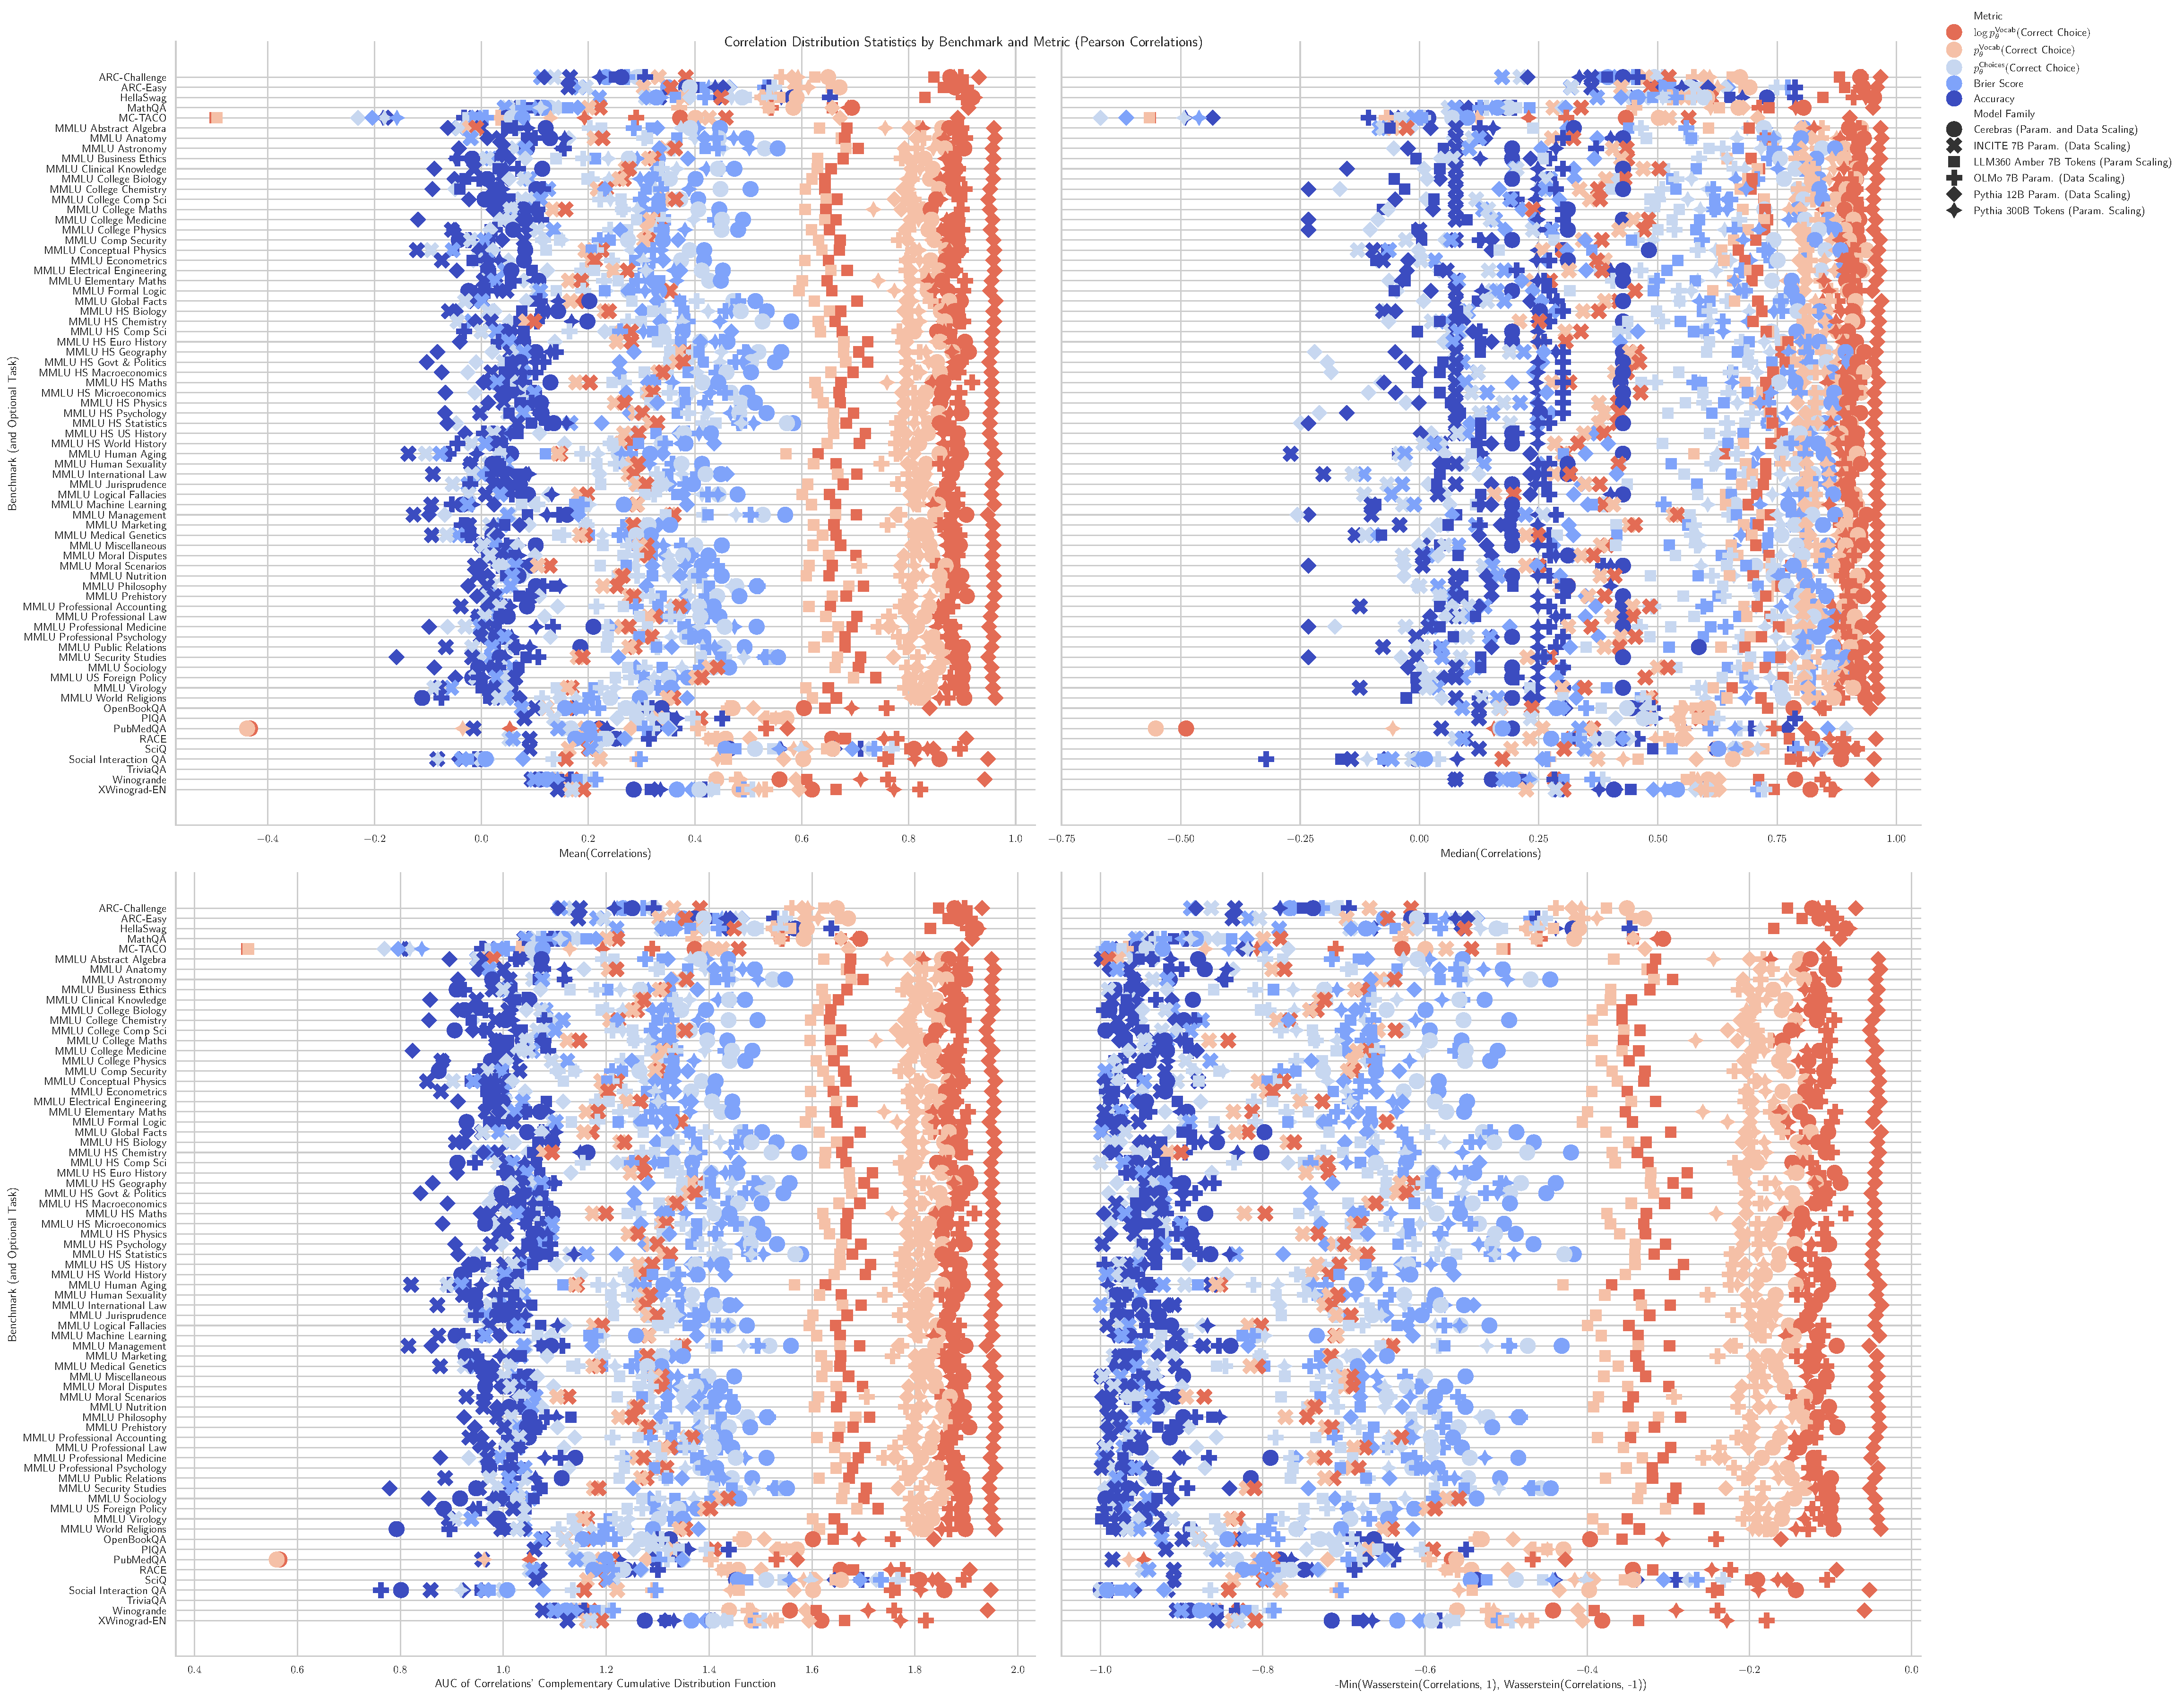
\includegraphics[width=\textwidth]{figures/correlations_between_scores_and_compute/correlation_distribution_statistics/correlation_metric=pearson/benchmark_vs_pearson_correlation_distribution_statistics_by_model_family_by_metric.pdf}
    \caption{\textbf{Statistics for empirical distributions of correlations between scores and compute for all benchmarks and model families.} These correlation values were computed with Pearson correlation and are consistent with the main text's results computed with Spearman correlation (Fig. \ref{fig:compute_score_distribution_statistics_spearman}): The sequence of transformations from $\log p_{\theta}^{\text{Vocab}}(\text{Correct Choice}) \rightarrow p_{\theta}^{\text{Vocab}}(\text{Correct Choice}) \rightarrow p_{\theta}^{\text{Choices}}(\text{Correct Choice}) \rightarrow \text{Accuracy}$ degrades predictability.}
     \label{app:fig:compute_score_distribution_statistics_pearson}
\end{figure}

\clearpage
\subsection{Spearman Correlations}

\begin{figure}[h!]
    \centering
    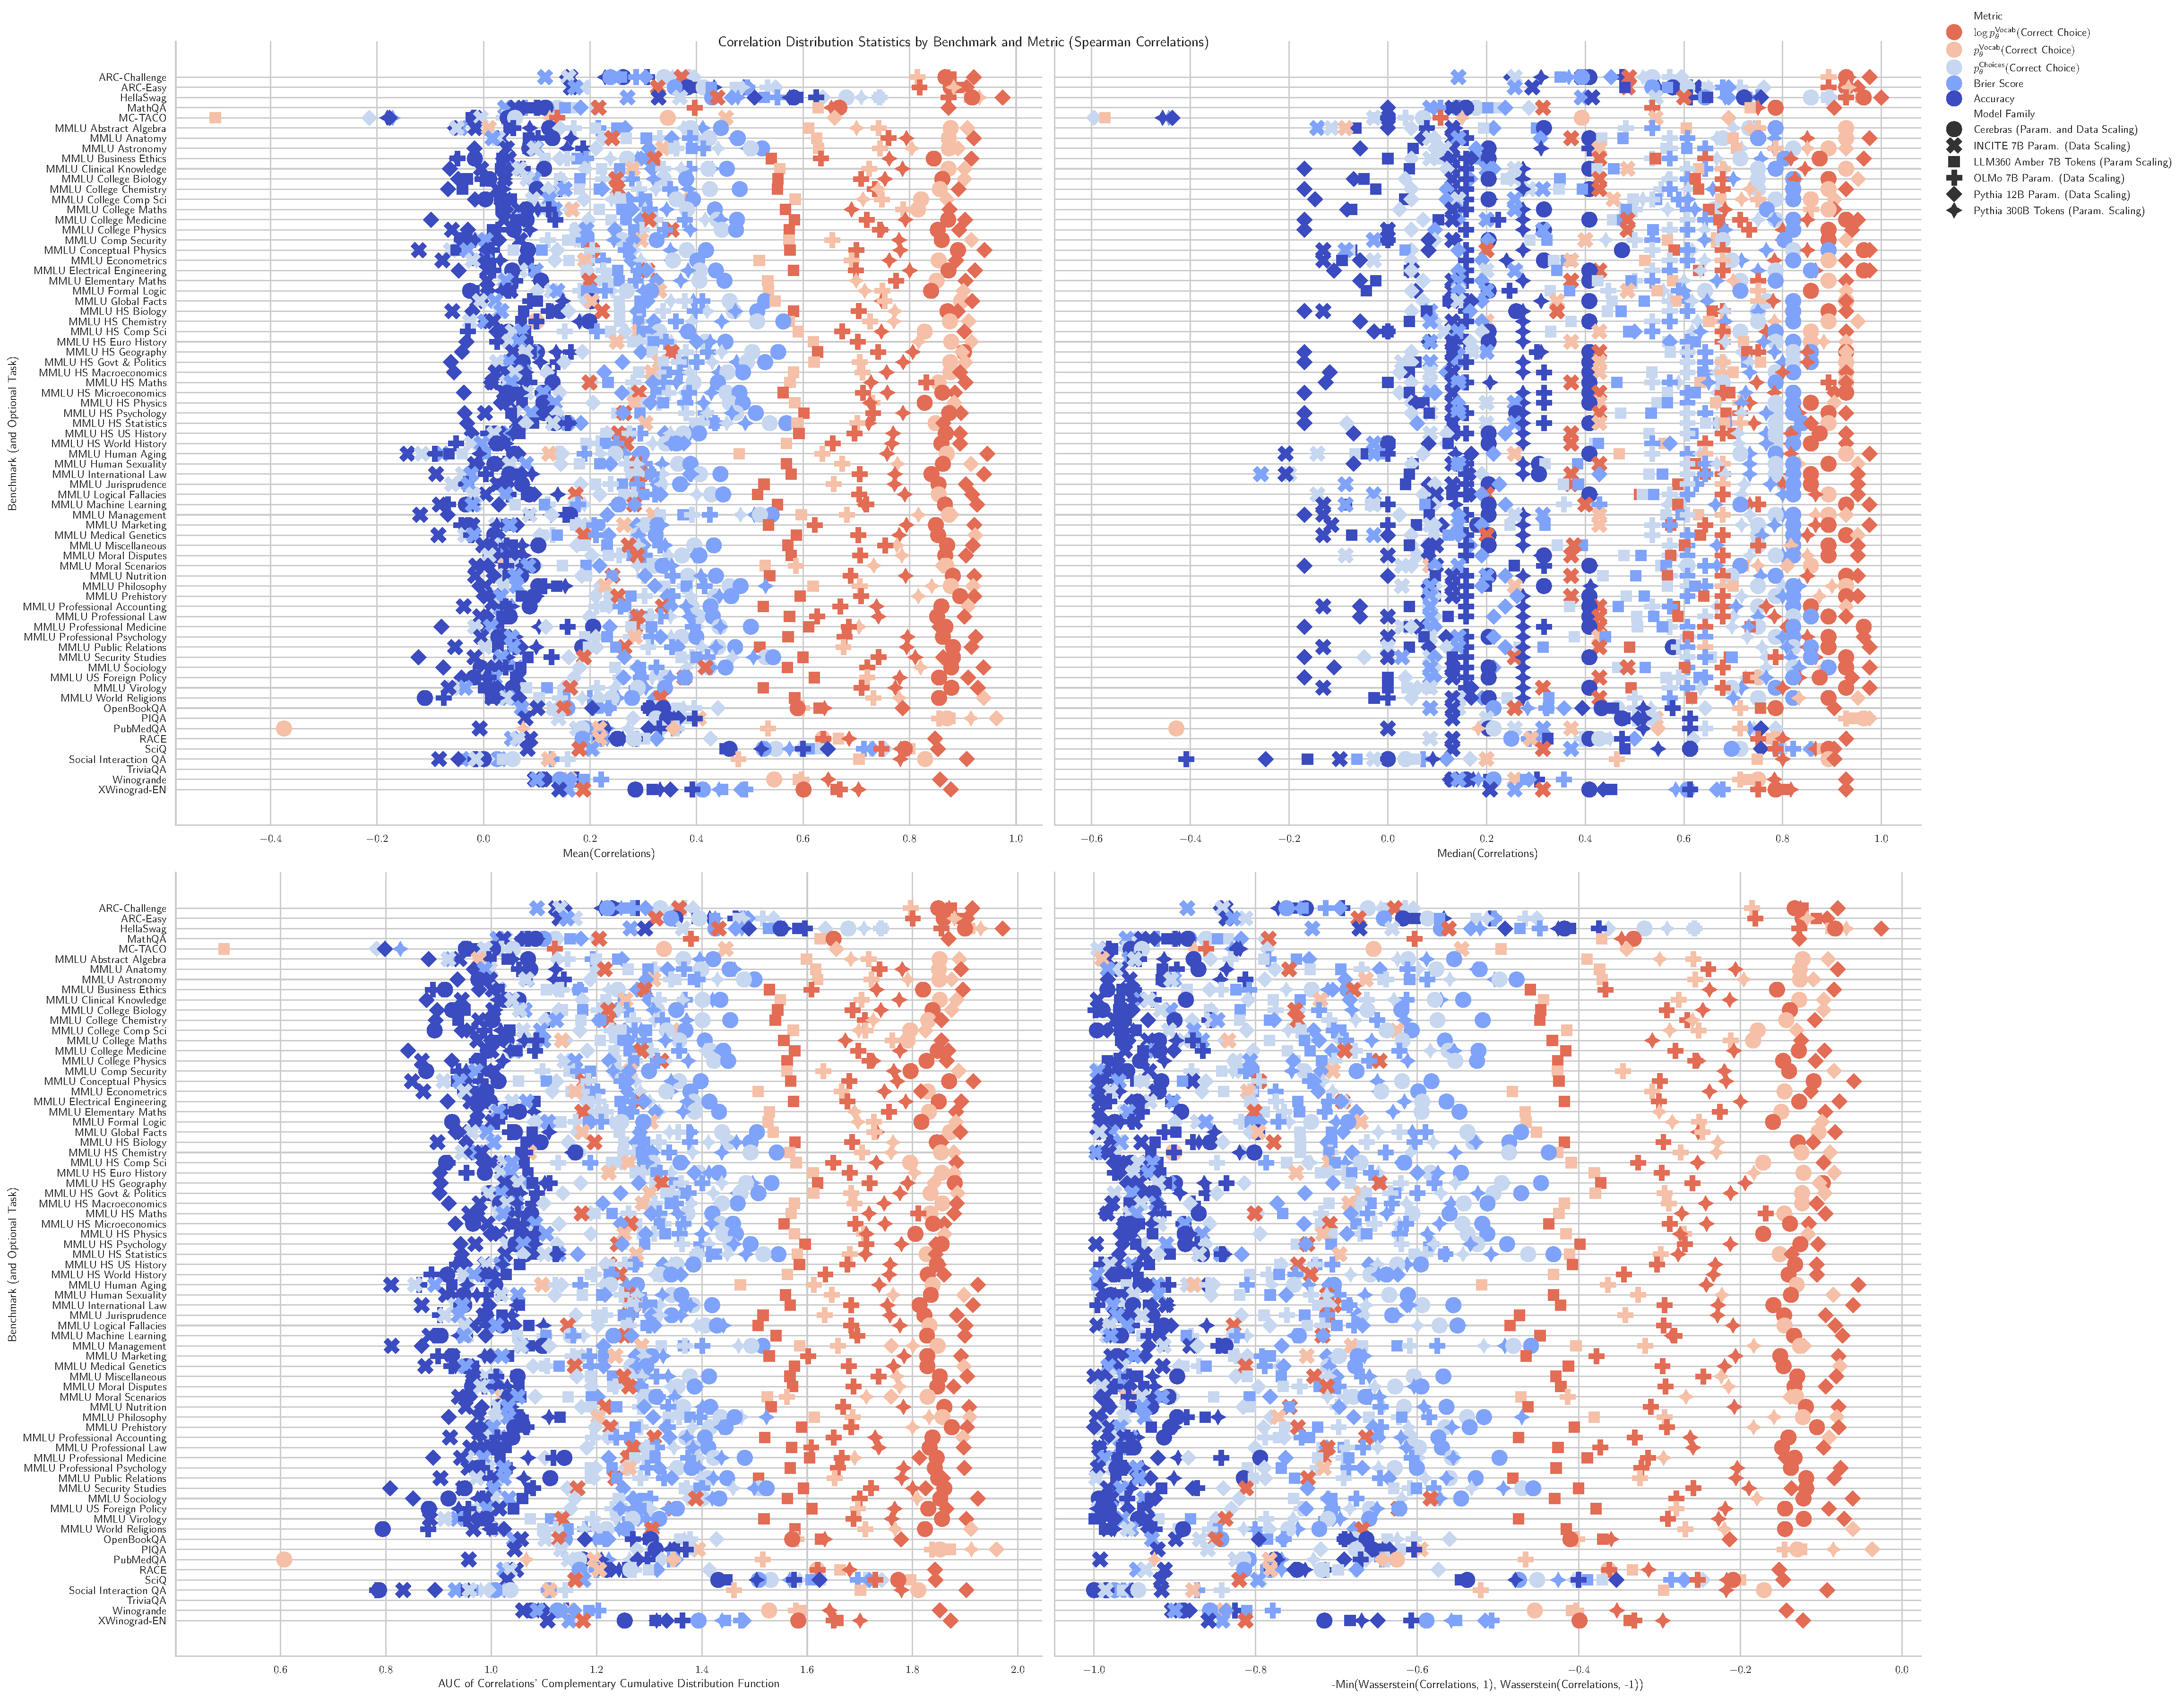
\includegraphics[width=\textwidth]{figures/correlations_between_scores_and_compute/correlation_distribution_statistics/correlation_metric=spearman/benchmark_vs_spearman_correlation_distribution_statistics_by_model_family_by_metric.pdf}
    \caption{\textbf{Statistics for empirical distributions of correlations between scores and compute for all benchmarks and model families.} These correlation values were computed with Spearman correlation. The sequence of transformations from $\log p_{\theta}^{\text{Vocab}}(\text{Correct Choice}) \rightarrow p_{\theta}^{\text{Vocab}}(\text{Correct Choice}) \rightarrow p_{\theta}^{\text{Choices}}(\text{Correct Choice}) \rightarrow \text{Accuracy}$ degrades predictability.}
    \label{app:fig:compute_score_distribution_statistics_spearman}
\end{figure}

\clearpage
\subsection{Kendall Correlations}

\begin{figure}[h!]
    \centering
    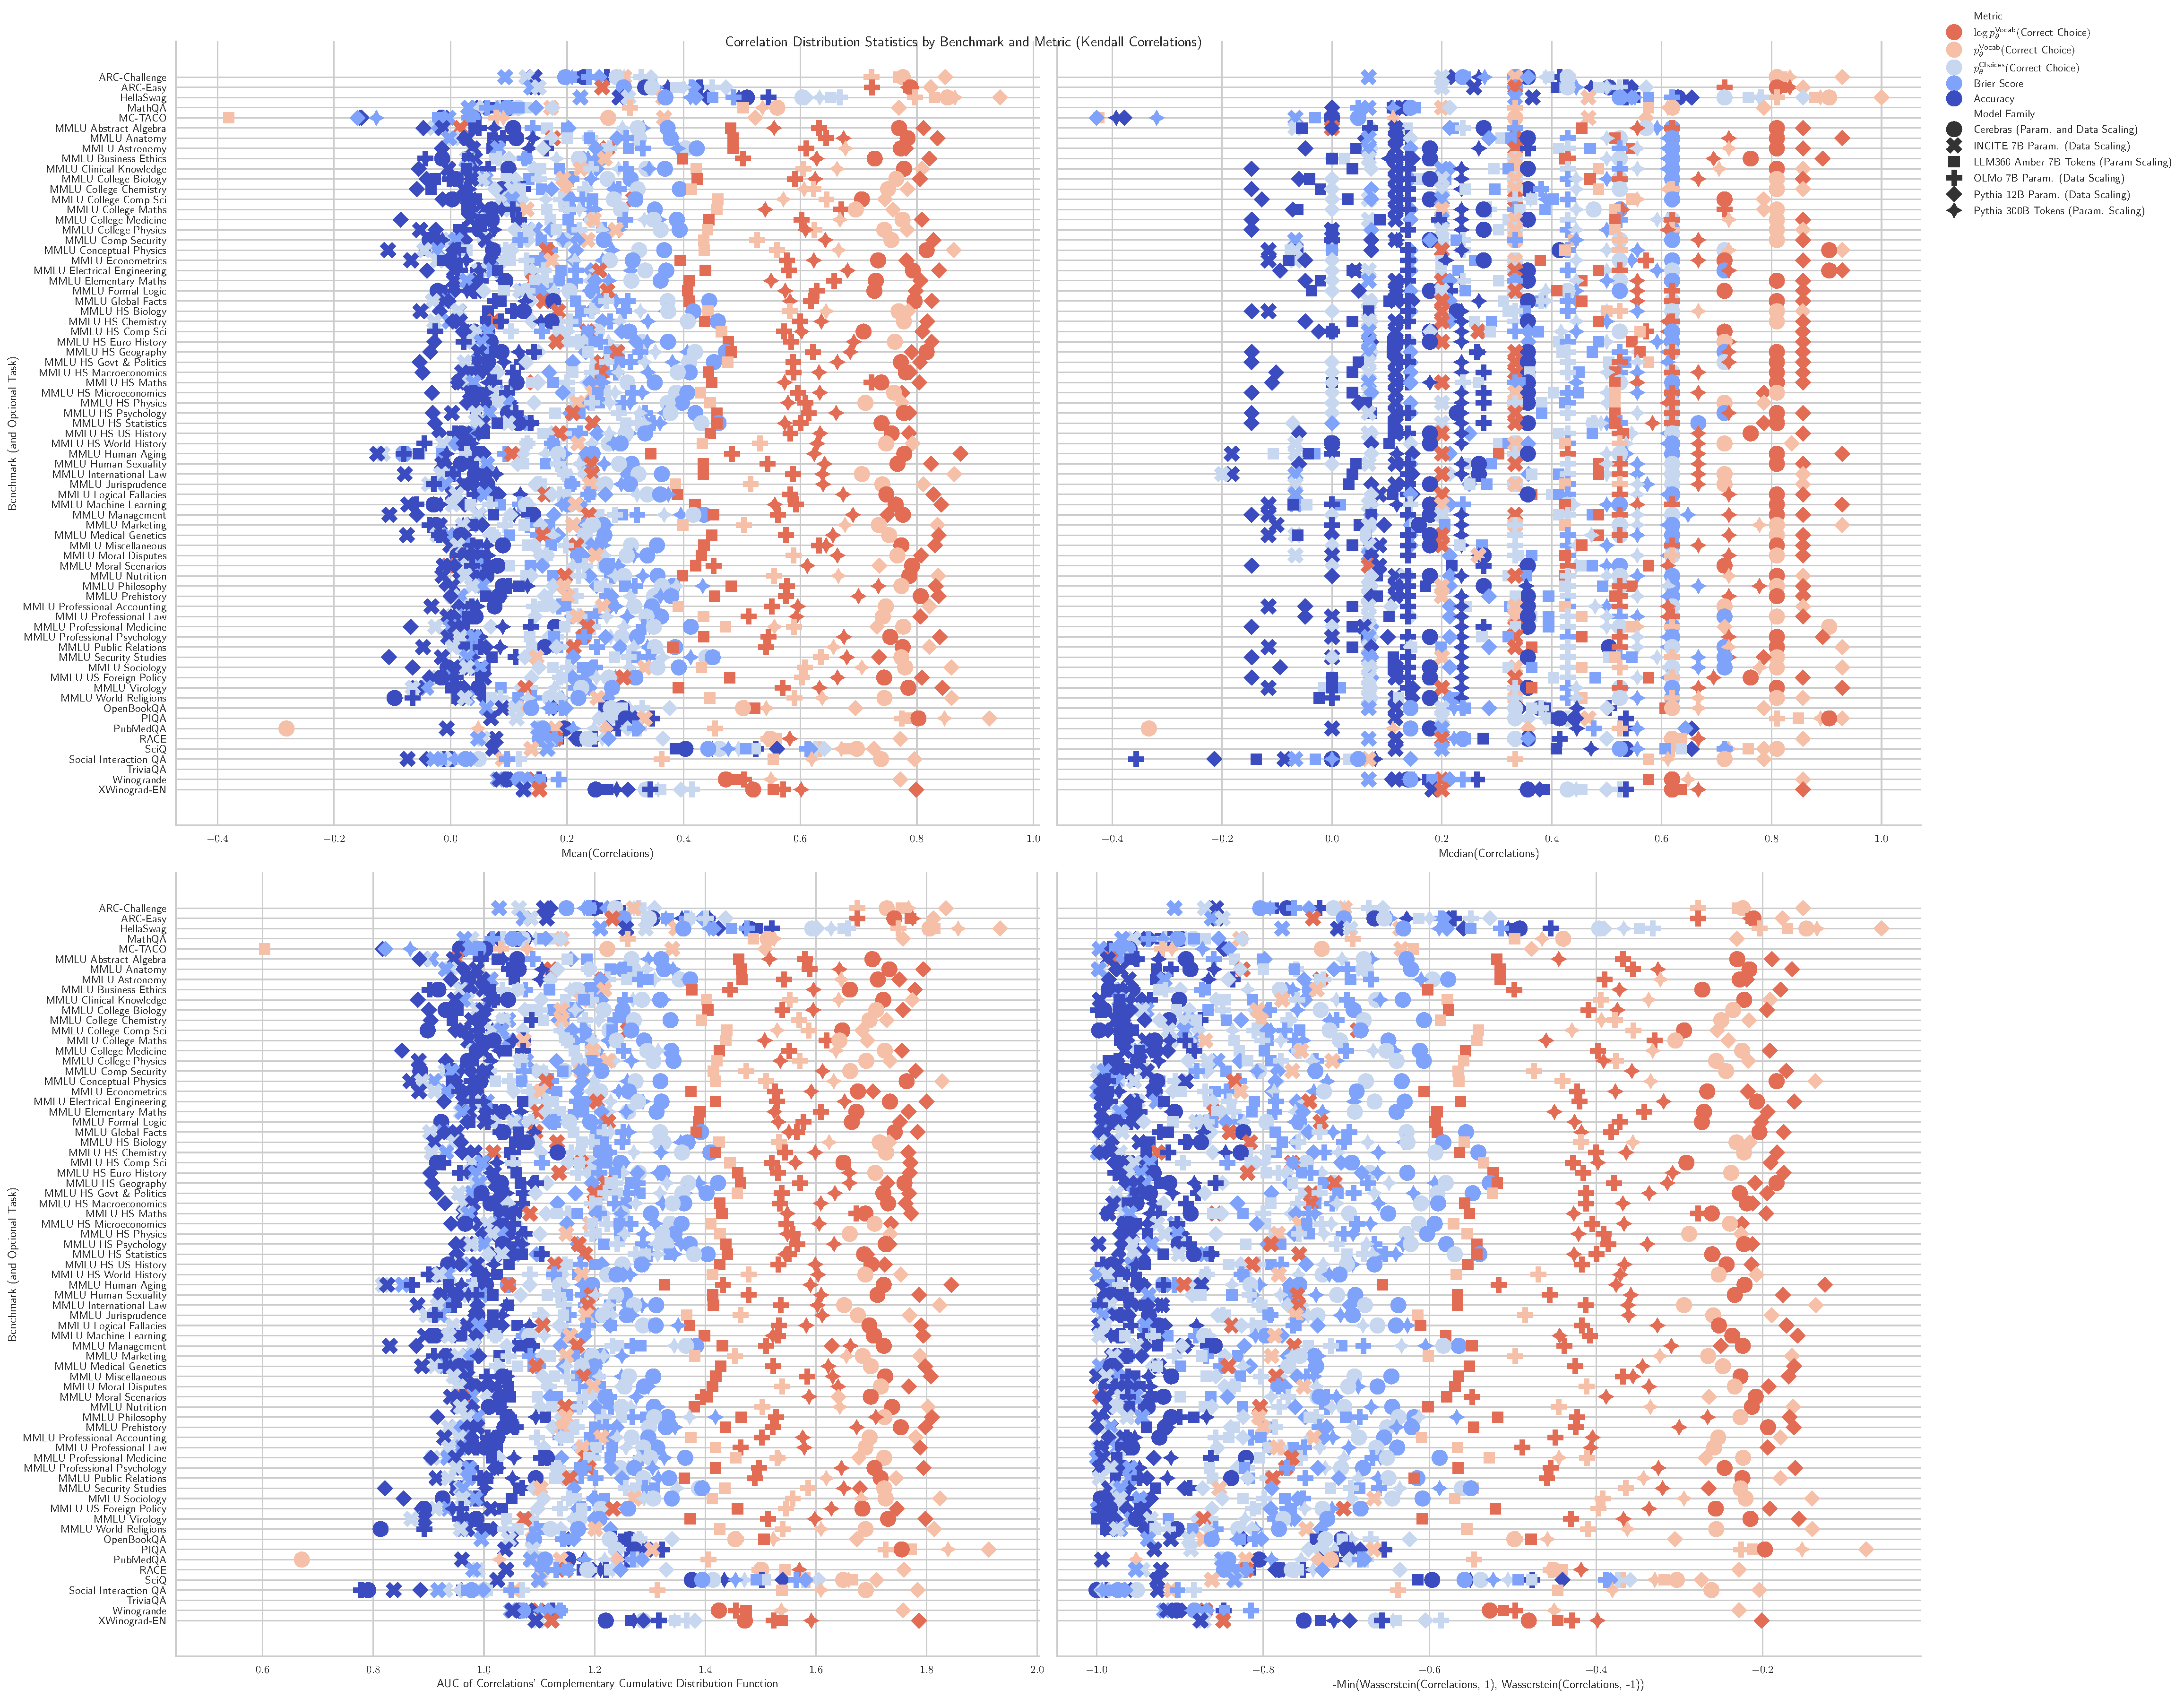
\includegraphics[width=\textwidth]{figures/correlations_between_scores_and_compute/correlation_distribution_statistics/correlation_metric=kendall/benchmark_vs_kendall_correlation_distribution_statistics_by_model_family_by_metric.pdf}
    \caption{\textbf{Statistics for empirical distributions of correlations between scores and compute for all benchmarks and model families.} These correlation values were computed with Kendall correlation and are consistent with the main text's results computed with Spearman correlation (Fig. \ref{fig:compute_score_distribution_statistics_spearman}): The sequence of transformations from $\log p_{\theta}^{\text{Vocab}}(\text{Correct Choice}) \rightarrow p_{\theta}^{\text{Vocab}}(\text{Correct Choice}) \rightarrow p_{\theta}^{\text{Choices}}(\text{Correct Choice}) \rightarrow \text{Accuracy}$ degrades predictability.}
    \label{app:fig:compute_score_distribution_statistics_kendall}
\end{figure}


% \clearpage
\section{Per-Benchmark Score-Compute Correlation Distributions}
\label{app:sec:additional_score_compute_correlation_distributions}


\subsection{NLP Benchmark: ARC Challenge \cite{clark2018arc}}

\begin{figure}[h!]
    \centering
    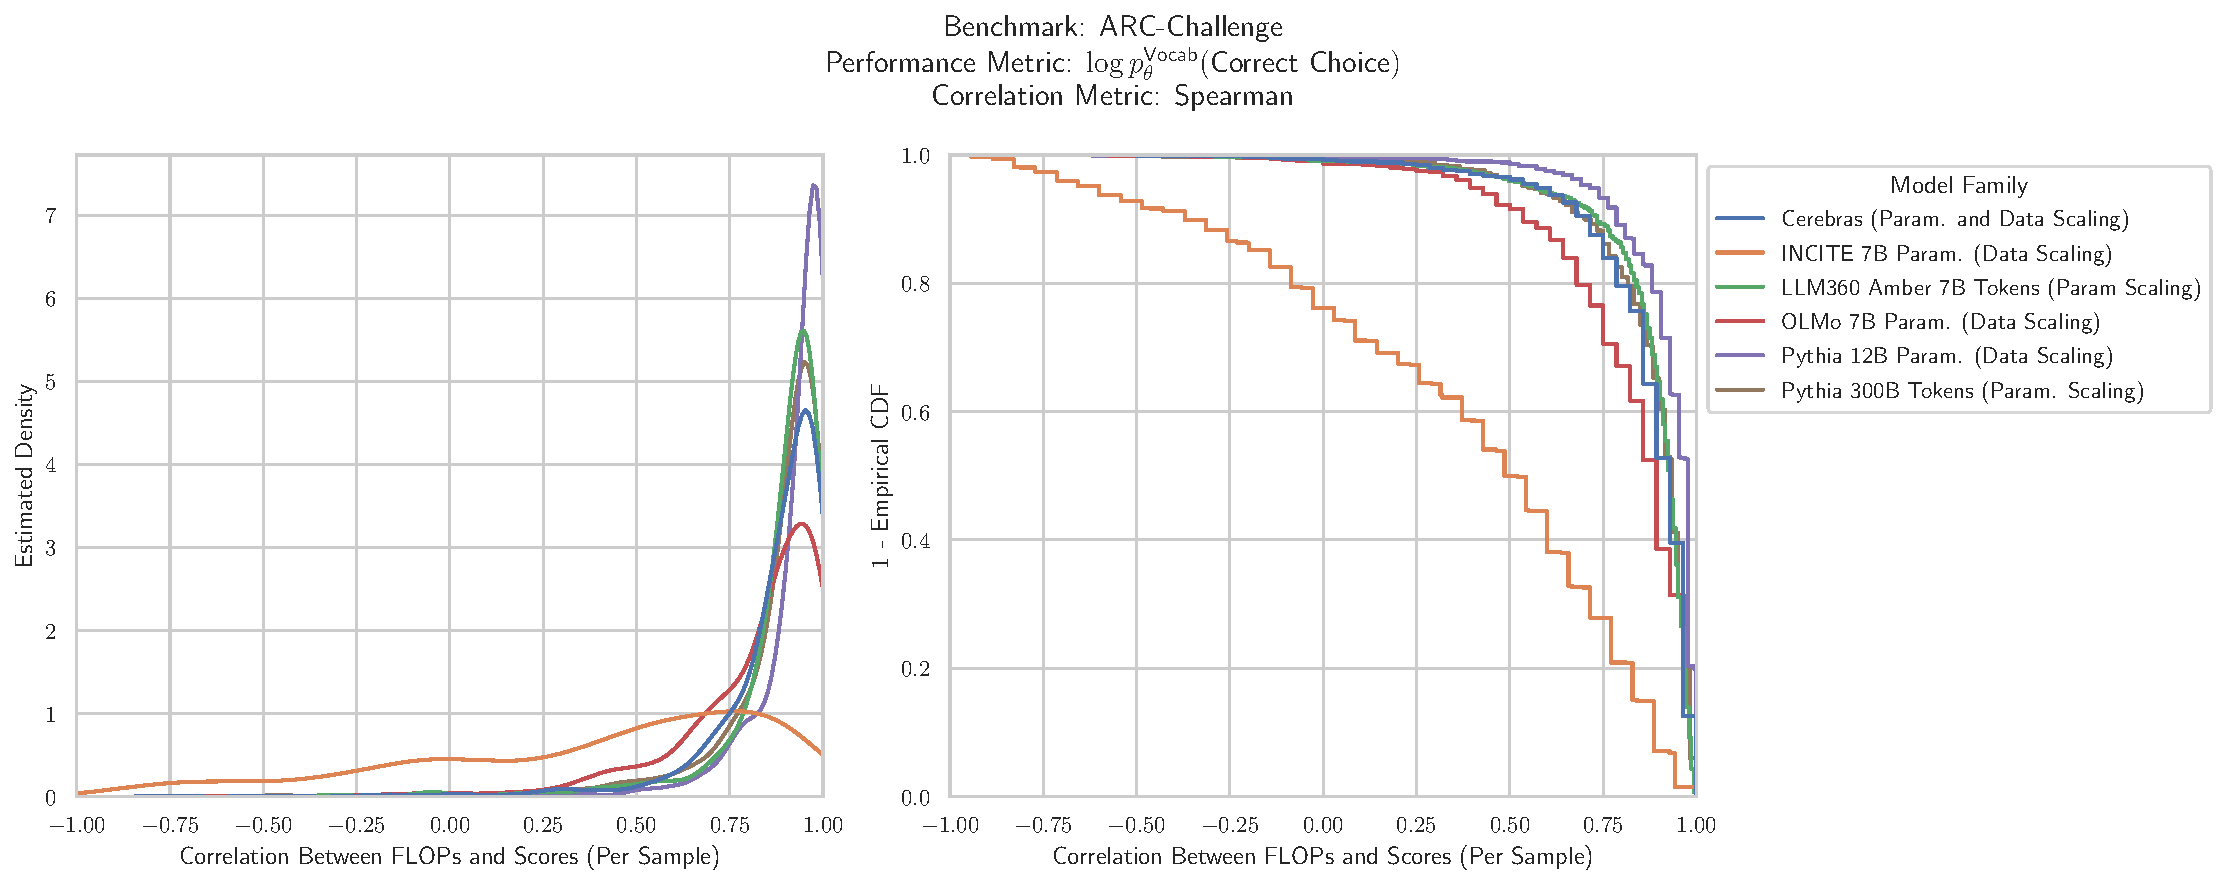
\includegraphics[width=\textwidth]{figures/correlations_between_scores_and_compute/correlation_distributions/arc_challenge/arc_challenge_log_prob_vocab_correct_kde_and_ecdf_vs_correlation_score_by_model_family_correlation_metric=spearman.pdf}
    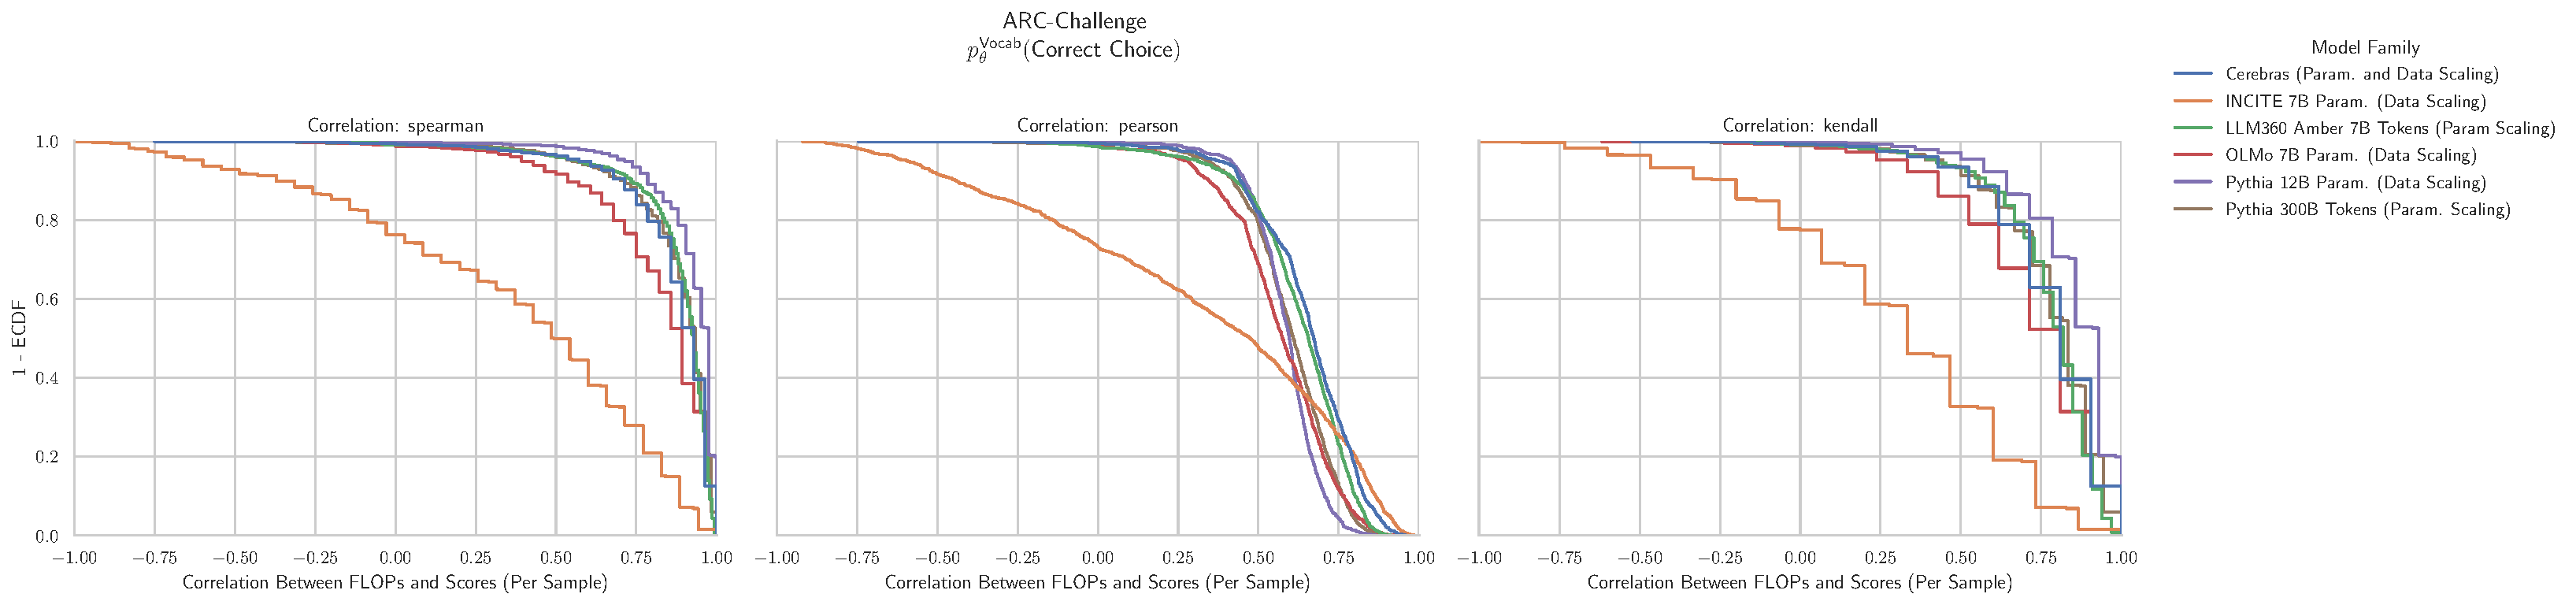
\includegraphics[width=\textwidth]{figures/correlations_between_scores_and_compute/correlation_distributions/arc_challenge/arc_challenge_prob_correct_vocab_ecdf_vs_correlation_score_by_modelfamily_split_correlation_metric.pdf}
    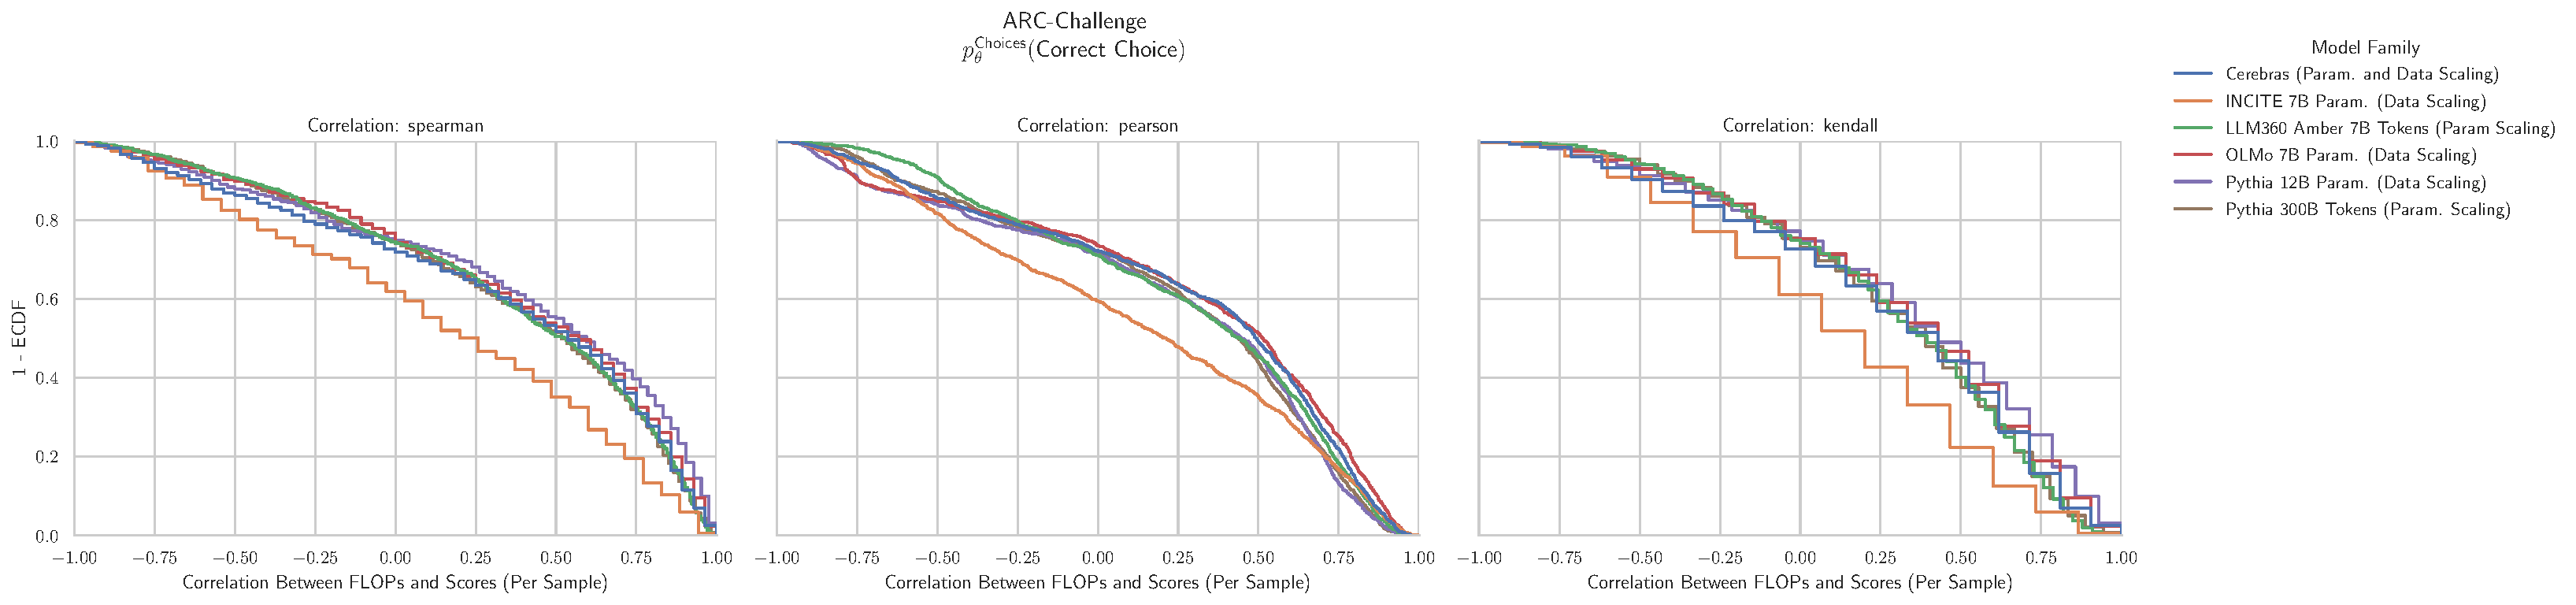
\includegraphics[width=\textwidth]{figures/correlations_between_scores_and_compute/correlation_distributions/arc_challenge/arc_challenge_prob_correct_choices_ecdf_vs_correlation_score_by_modelfamily_split_correlation_metric.pdf}
    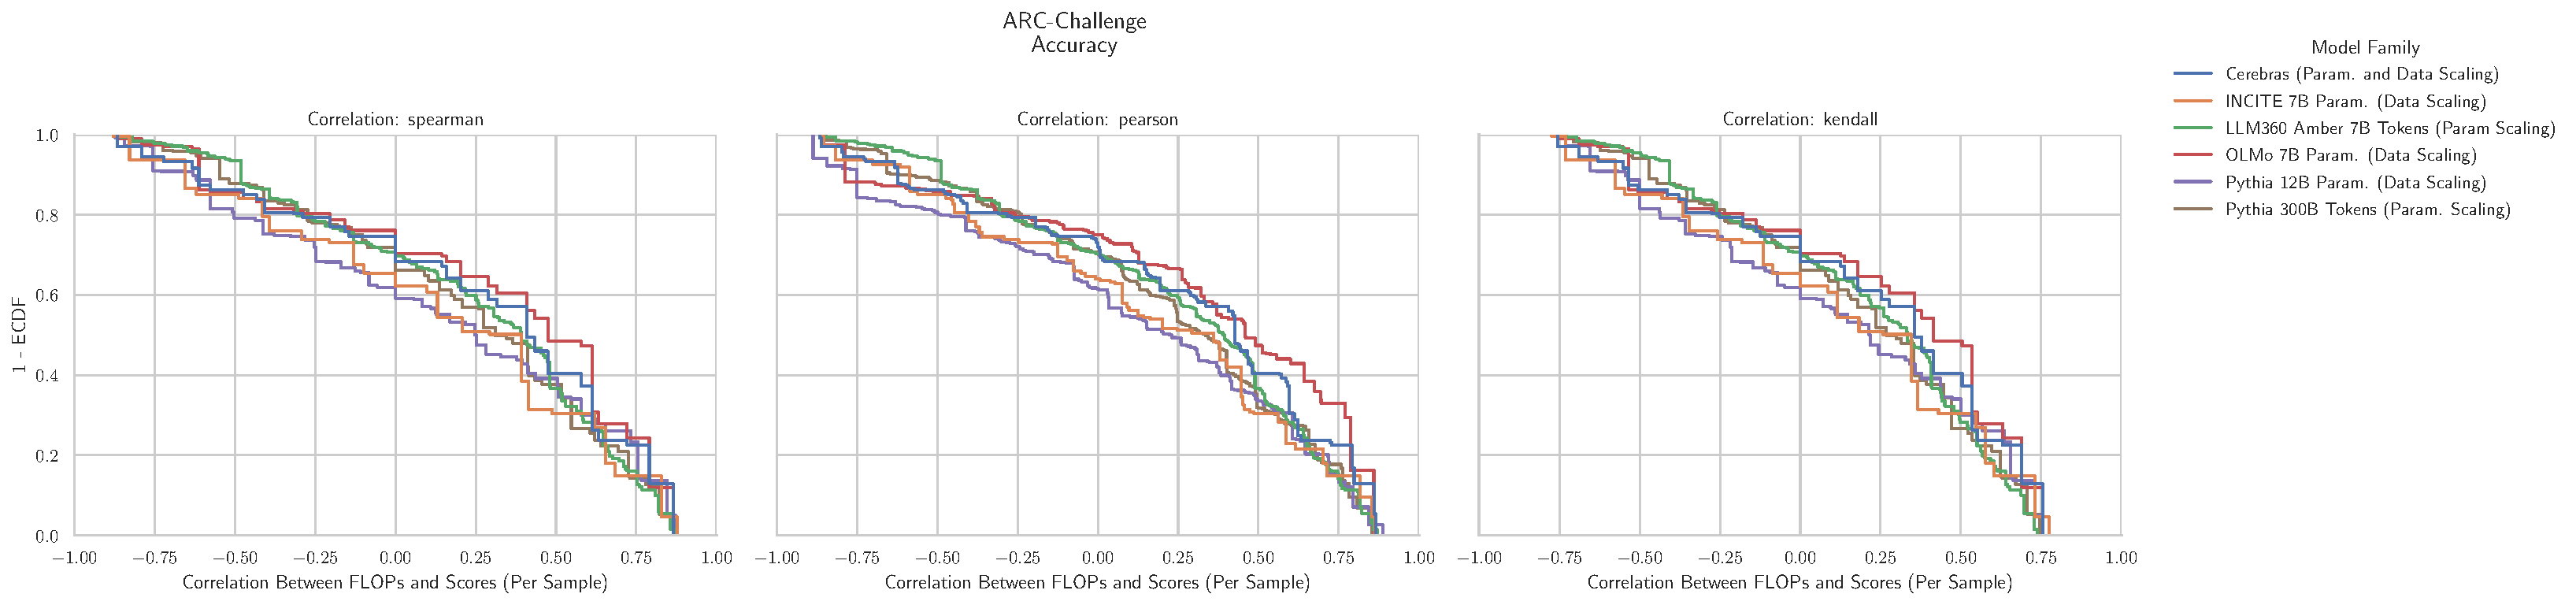
\includegraphics[width=\textwidth]{figures/correlations_between_scores_and_compute/correlation_distributions/arc_challenge/arc_challenge_acc_ecdf_vs_correlation_score_by_modelfamily_split_correlation_metric.pdf}
    \caption{\textbf{ARC Challenge: Downstream performance is computed via a sequence of transformations that deteriorate correlations between scores and pretraining compute.}}
    \label{app:fig:compute_score_distribution_arc_challenge}
\end{figure}



\clearpage
\subsection{NLP Benchmark: ARC Easy \cite{clark2018arc}}

\begin{figure}[h!]
    \centering
    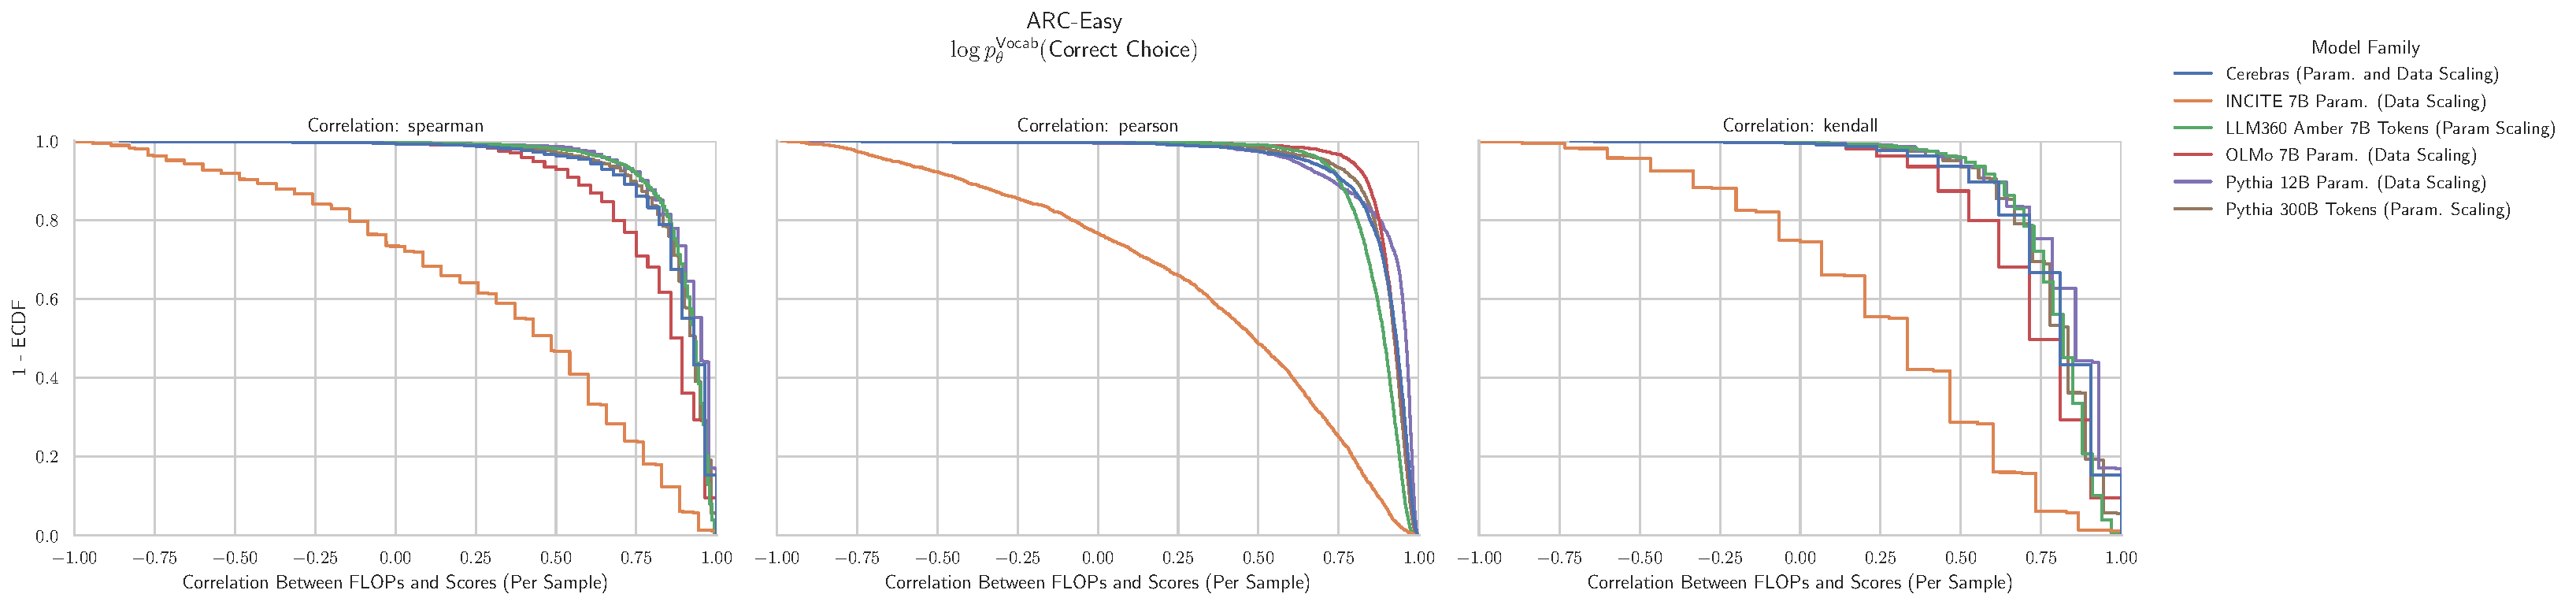
\includegraphics[width=\textwidth]{figures/correlations_between_scores_and_compute/correlation_distributions/arc_easy/arc_easy_log_likelihood_correct_ecdf_vs_correlation_score_by_modelfamily_split_correlation_metric.pdf}
    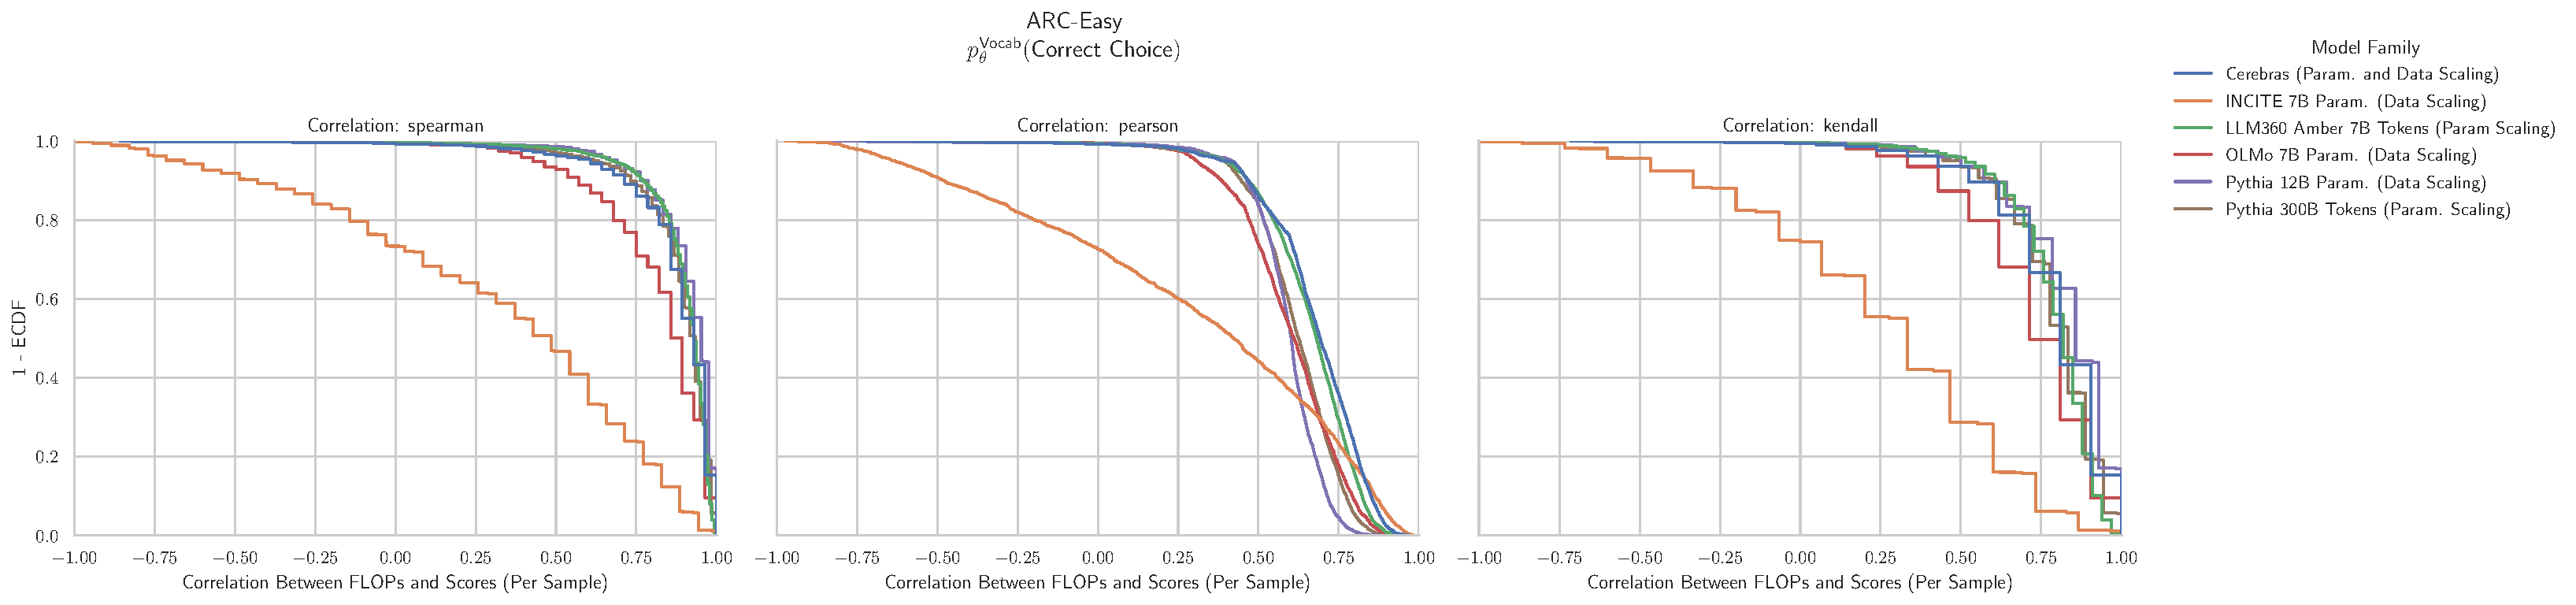
\includegraphics[width=\textwidth]{figures/correlations_between_scores_and_compute/correlation_distributions/arc_easy/arc_easy_prob_correct_vocab_ecdf_vs_correlation_score_by_modelfamily_split_correlation_metric.pdf}
    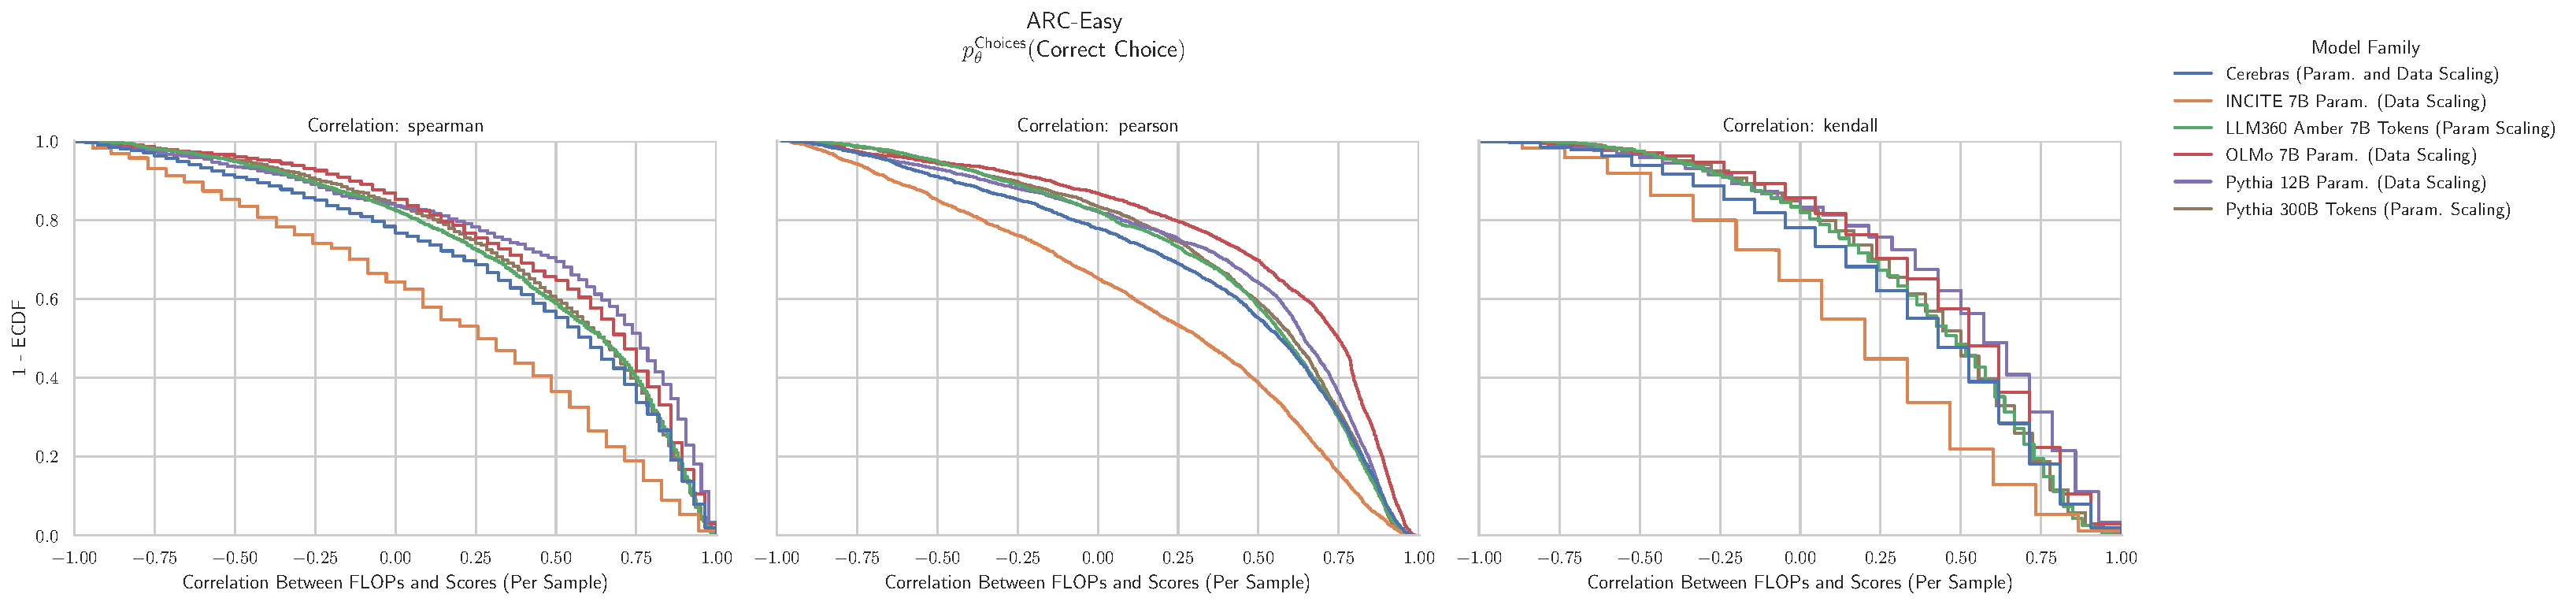
\includegraphics[width=\textwidth]{figures/correlations_between_scores_and_compute/correlation_distributions/arc_easy/arc_easy_prob_correct_choices_ecdf_vs_correlation_score_by_modelfamily_split_correlation_metric.pdf}
    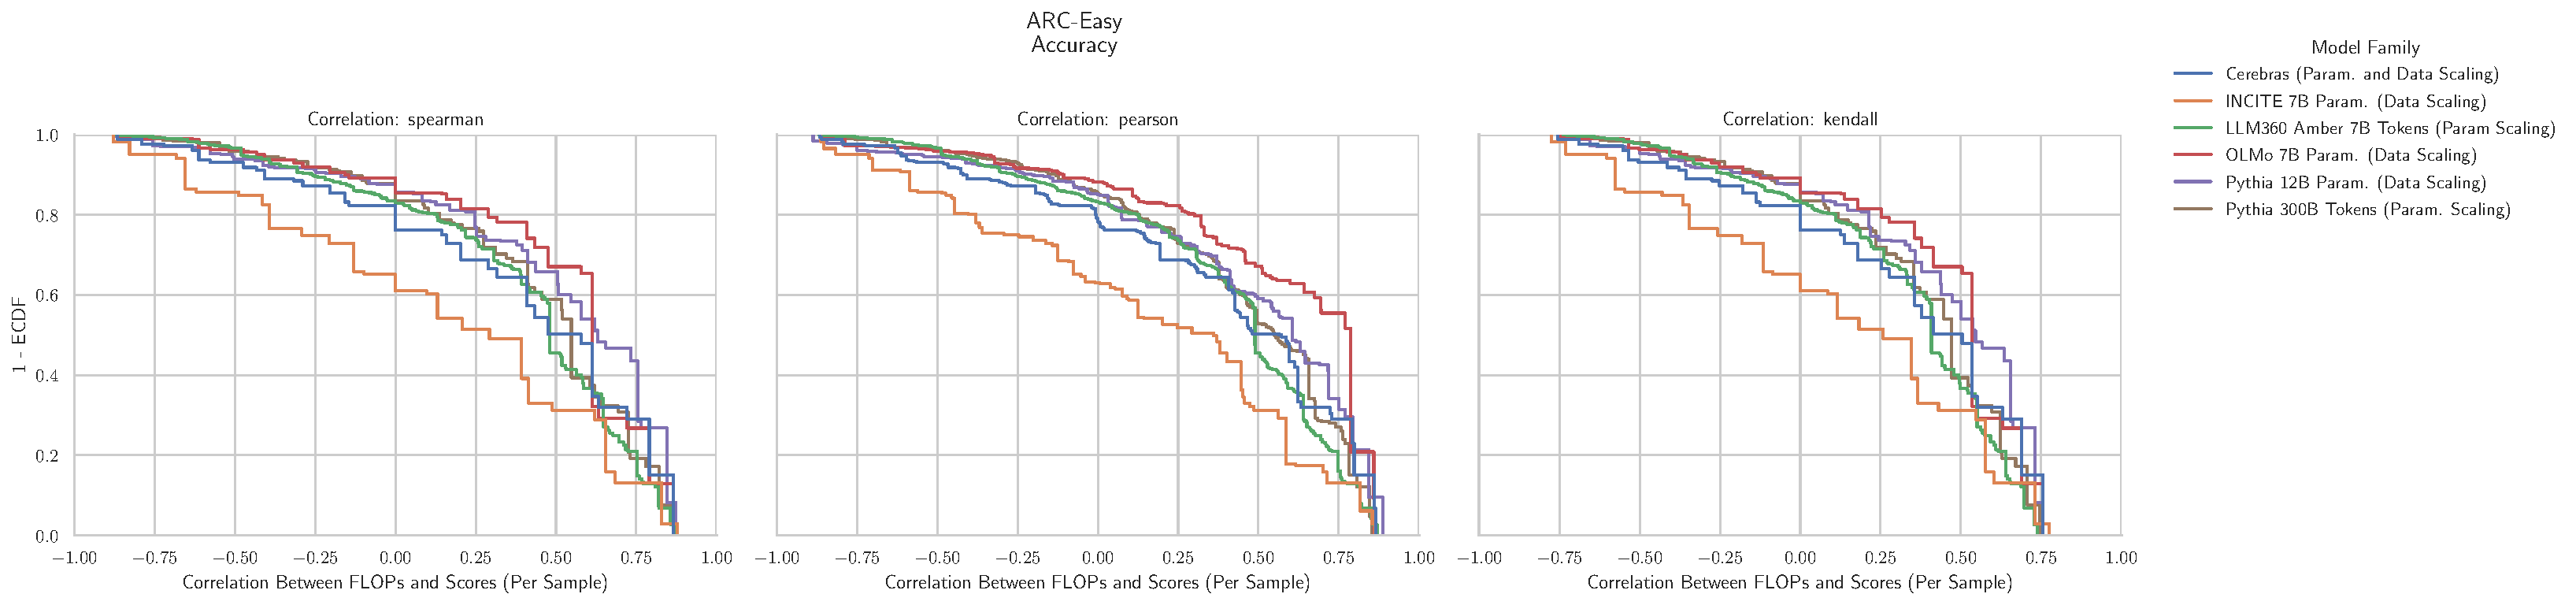
\includegraphics[width=\textwidth]{figures/correlations_between_scores_and_compute/correlation_distributions/arc_easy/arc_easy_acc_ecdf_vs_correlation_score_by_modelfamily_split_correlation_metric.pdf}
    \caption{\textbf{ARC Easy: Downstream performance is computed via a sequence of transformations that deteriorate correlations between scores and pretraining compute.}}
    \label{app:fig:compute_score_distribution_arc_easy}
\end{figure}

\clearpage
\subsection{NLP Benchmark: HellaSwag \cite{zellers2019hellaswag}}

\begin{figure}[h!]
    \centering
    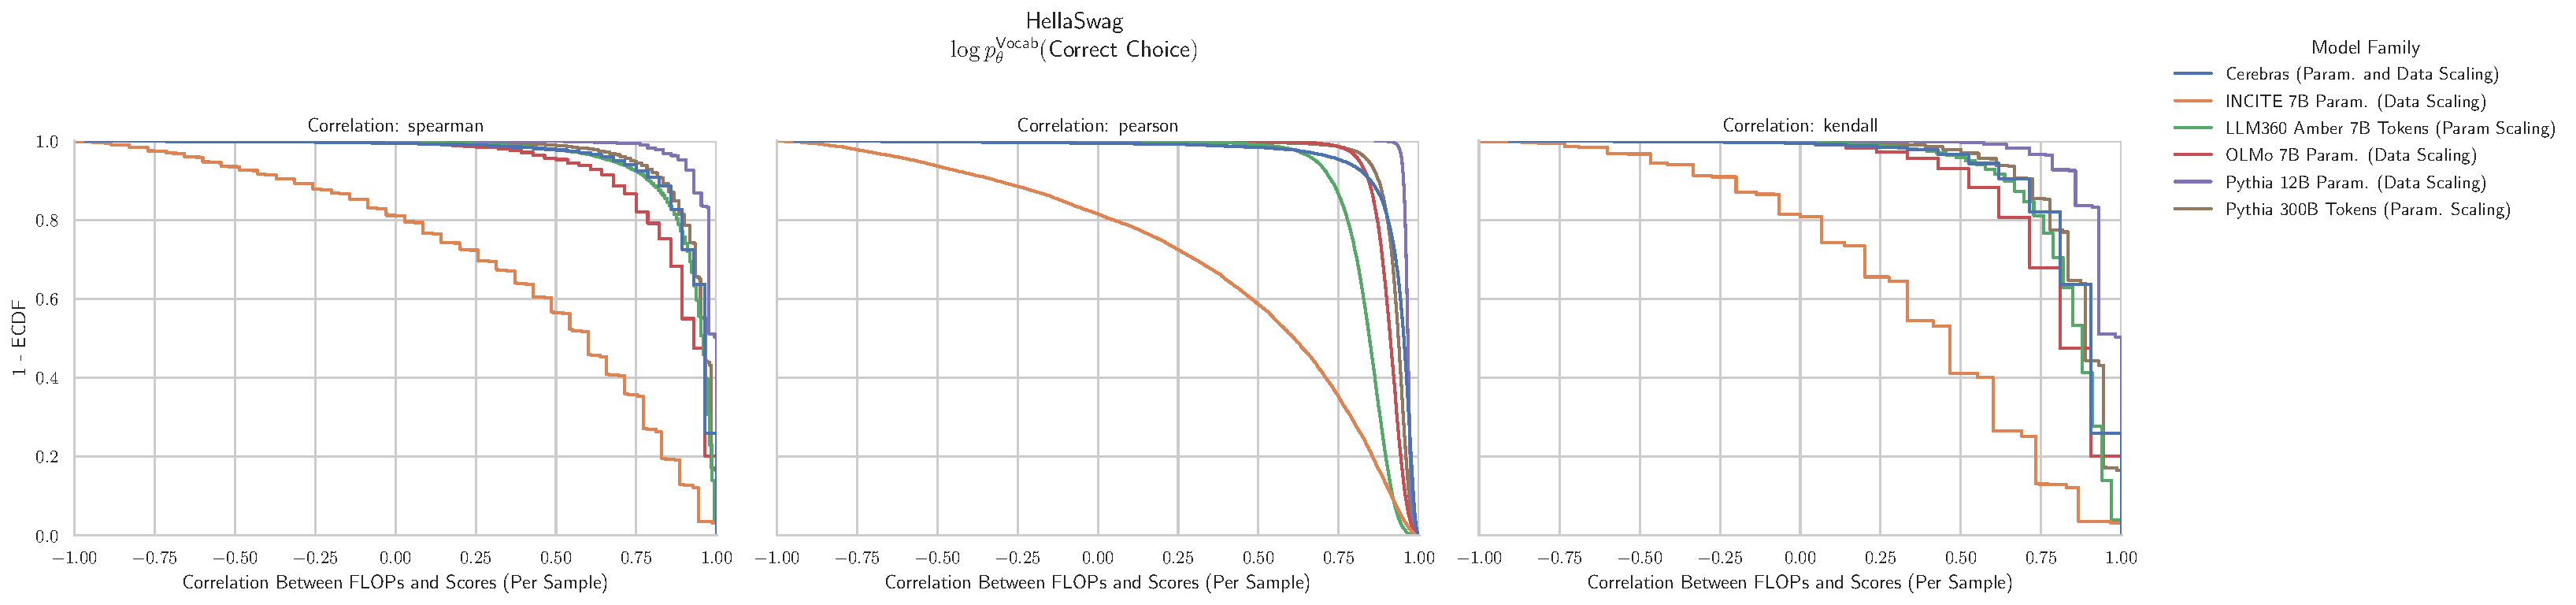
\includegraphics[width=\textwidth]{figures/correlations_between_scores_and_compute/correlation_distributions/hellaswag/hellaswag_log_likelihood_correct_ecdf_vs_correlation_score_by_modelfamily_split_correlation_metric.pdf}
    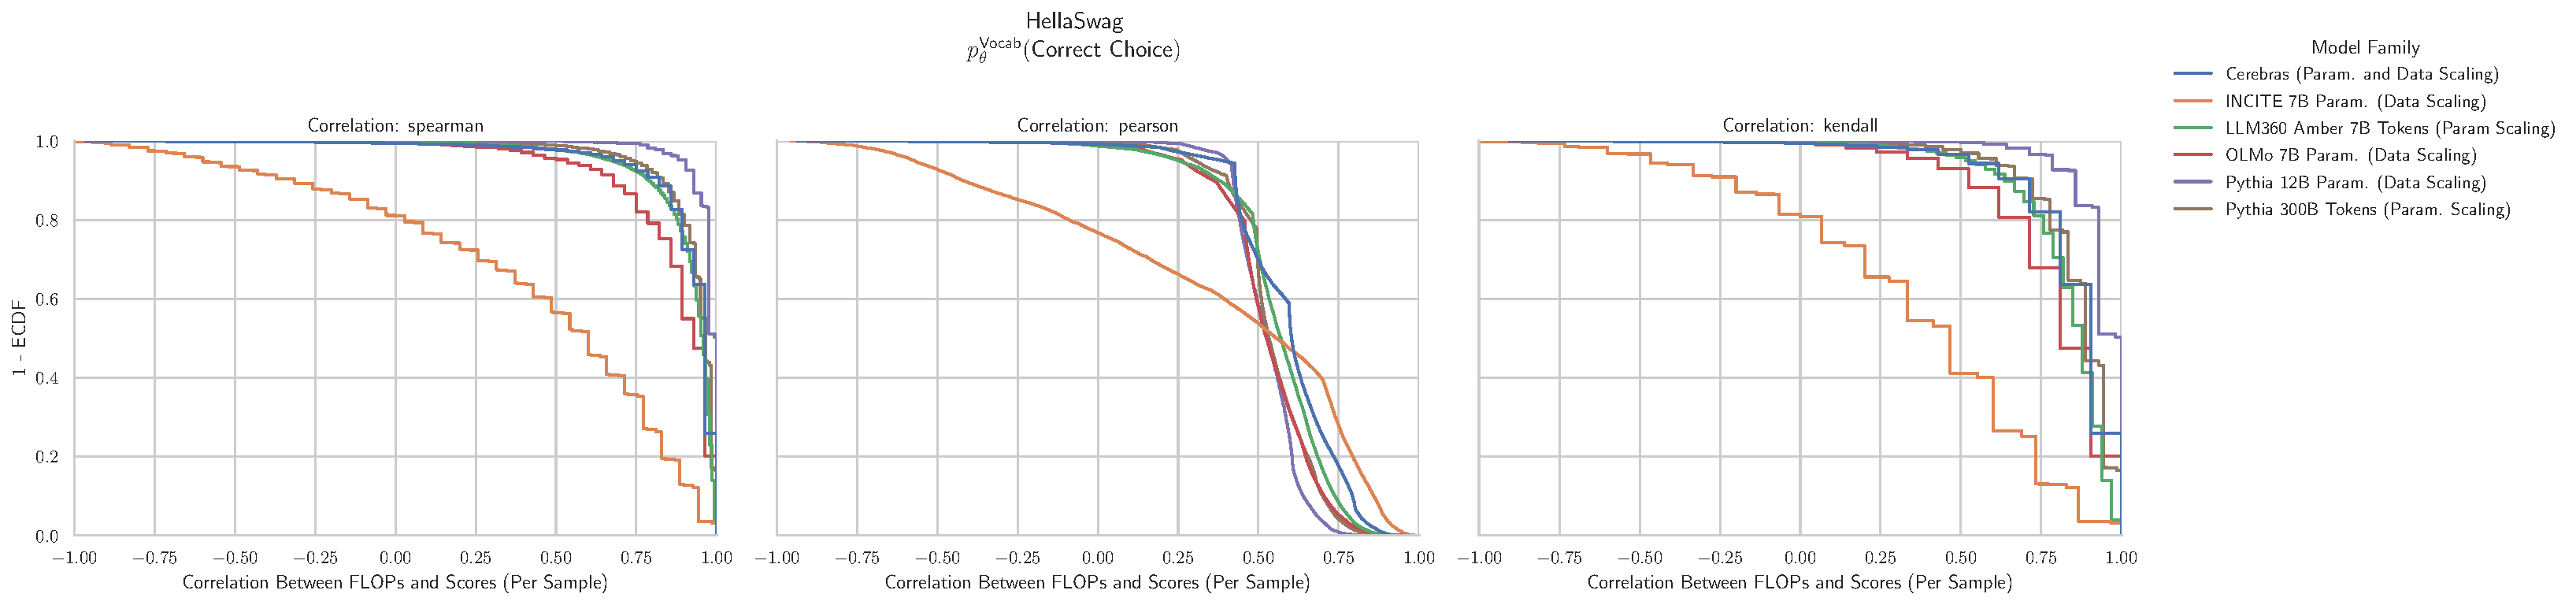
\includegraphics[width=\textwidth]{figures/correlations_between_scores_and_compute/correlation_distributions/hellaswag/hellaswag_prob_correct_vocab_ecdf_vs_correlation_score_by_modelfamily_split_correlation_metric.pdf}
    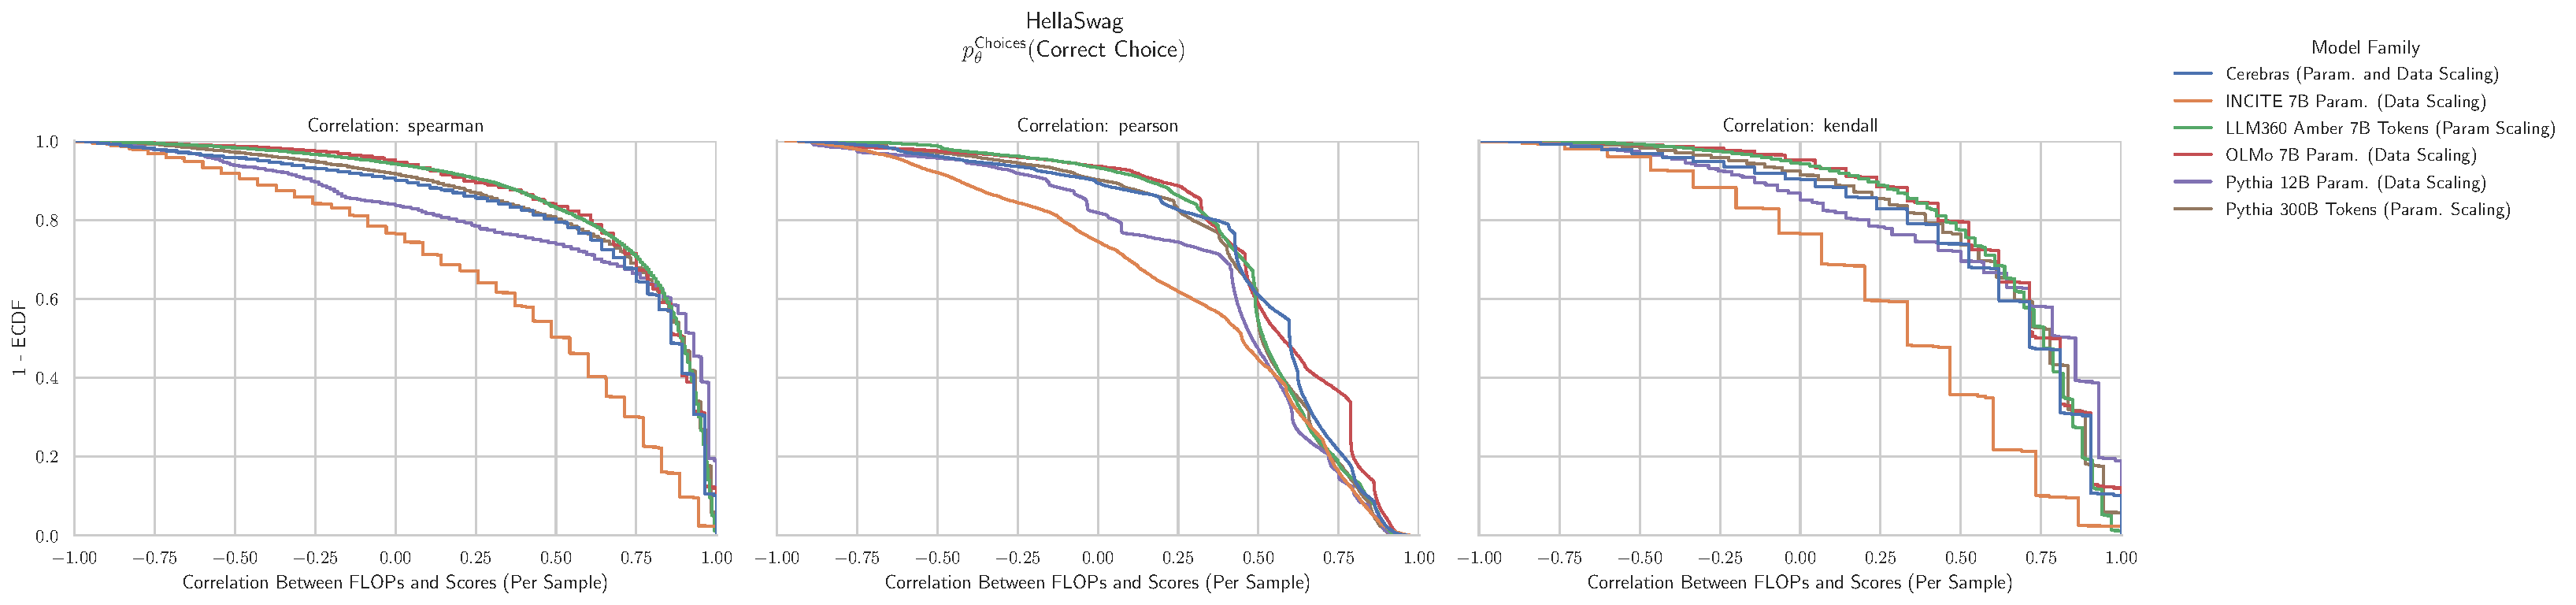
\includegraphics[width=\textwidth]{figures/correlations_between_scores_and_compute/correlation_distributions/hellaswag/hellaswag_prob_correct_choices_ecdf_vs_correlation_score_by_modelfamily_split_correlation_metric.pdf}
    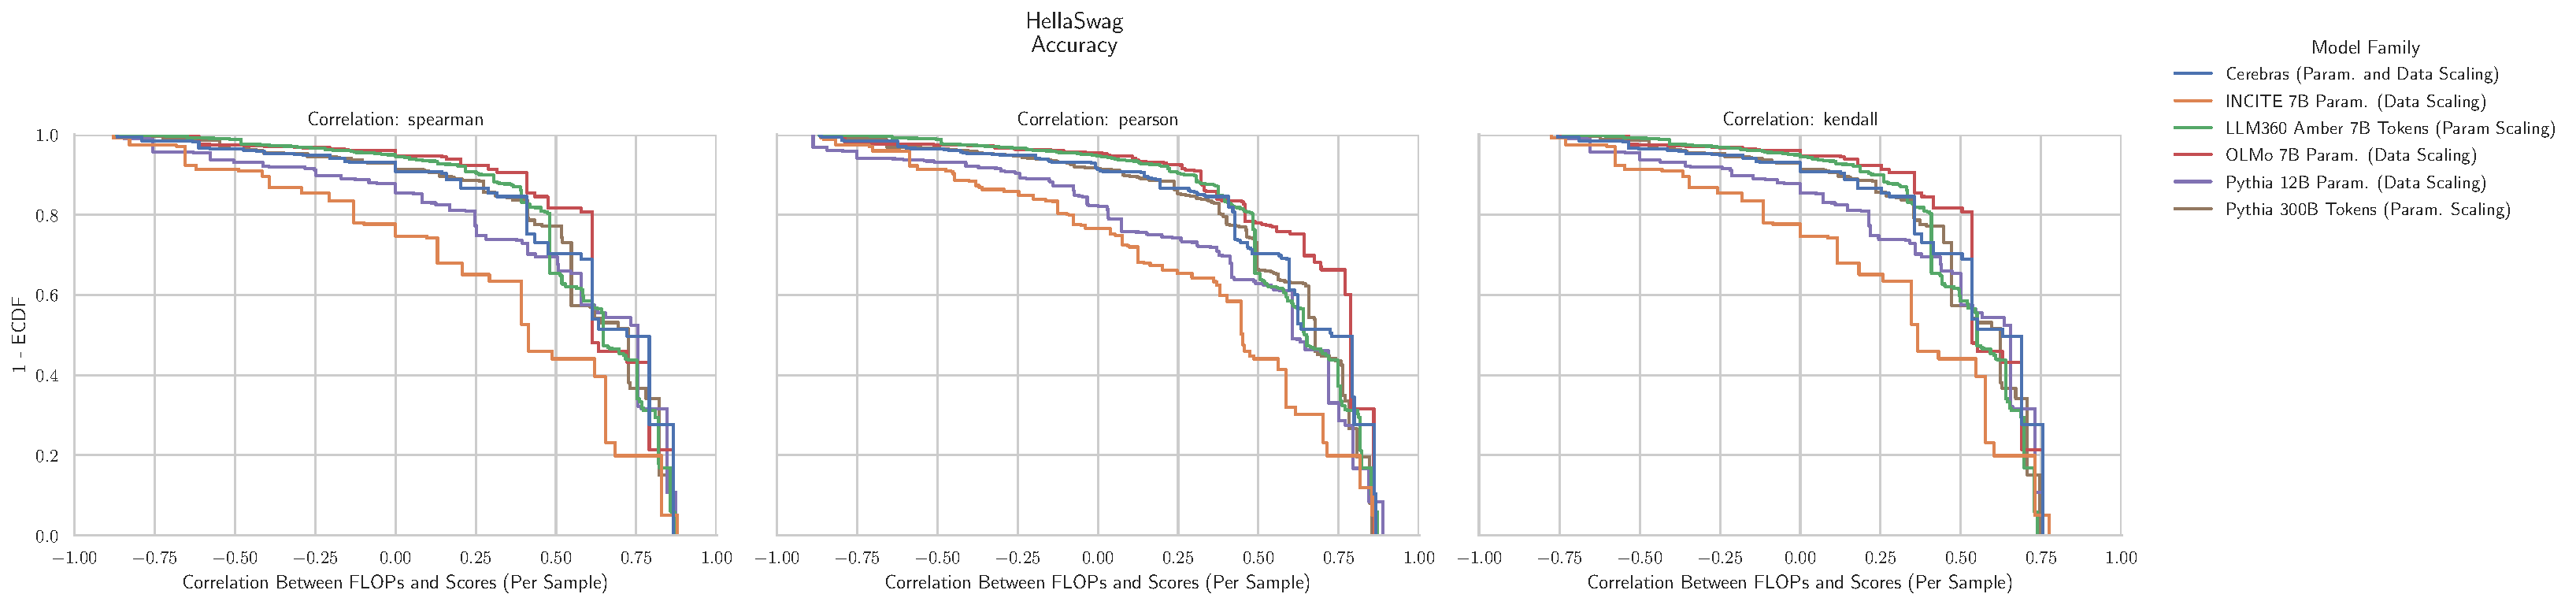
\includegraphics[width=\textwidth]{figures/correlations_between_scores_and_compute/correlation_distributions/hellaswag/hellaswag_acc_ecdf_vs_correlation_score_by_modelfamily_split_correlation_metric.pdf}
    \caption{\textbf{HellaSwag: Downstream performance is computed via a sequence of transformations that deteriorate correlations between scores and pretraining compute.}}
    \label{app:fig:compute_score_distribution_hellaswag}
\end{figure}


\clearpage
\subsection{NLP Benchmark: MathQA \cite{amini2019mathqa}}

\begin{figure}[h!]
    \centering
    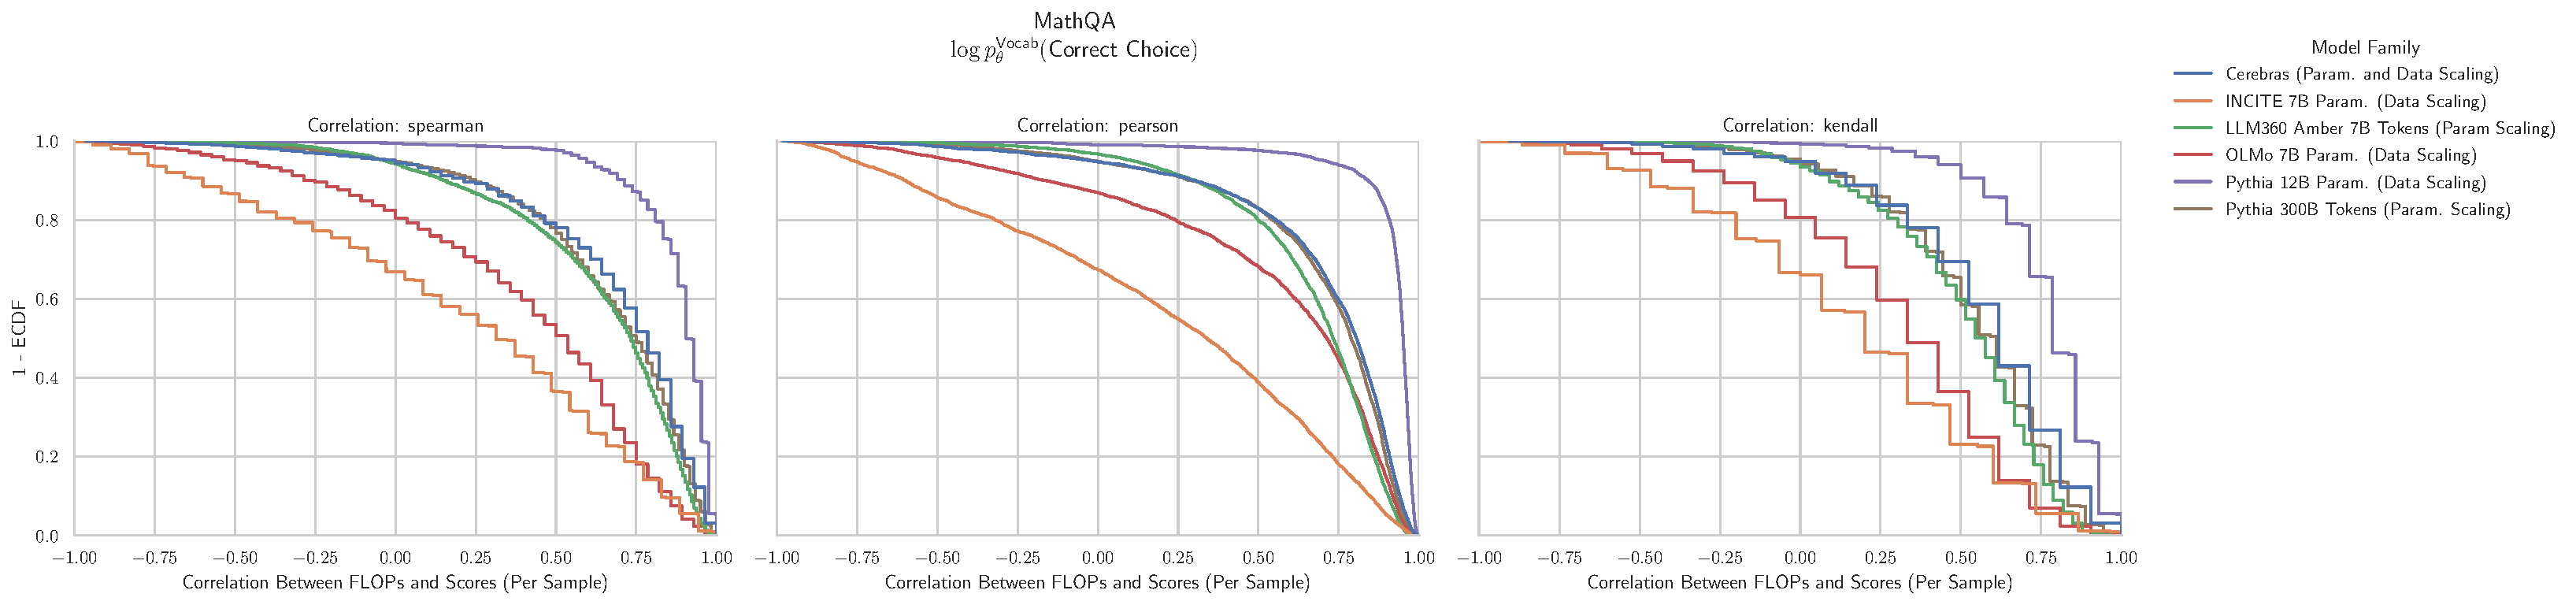
\includegraphics[width=\textwidth]{figures/correlations_between_scores_and_compute/correlation_distributions/mathqa/mathqa_log_likelihood_correct_ecdf_vs_correlation_score_by_modelfamily_split_correlation_metric.pdf}
    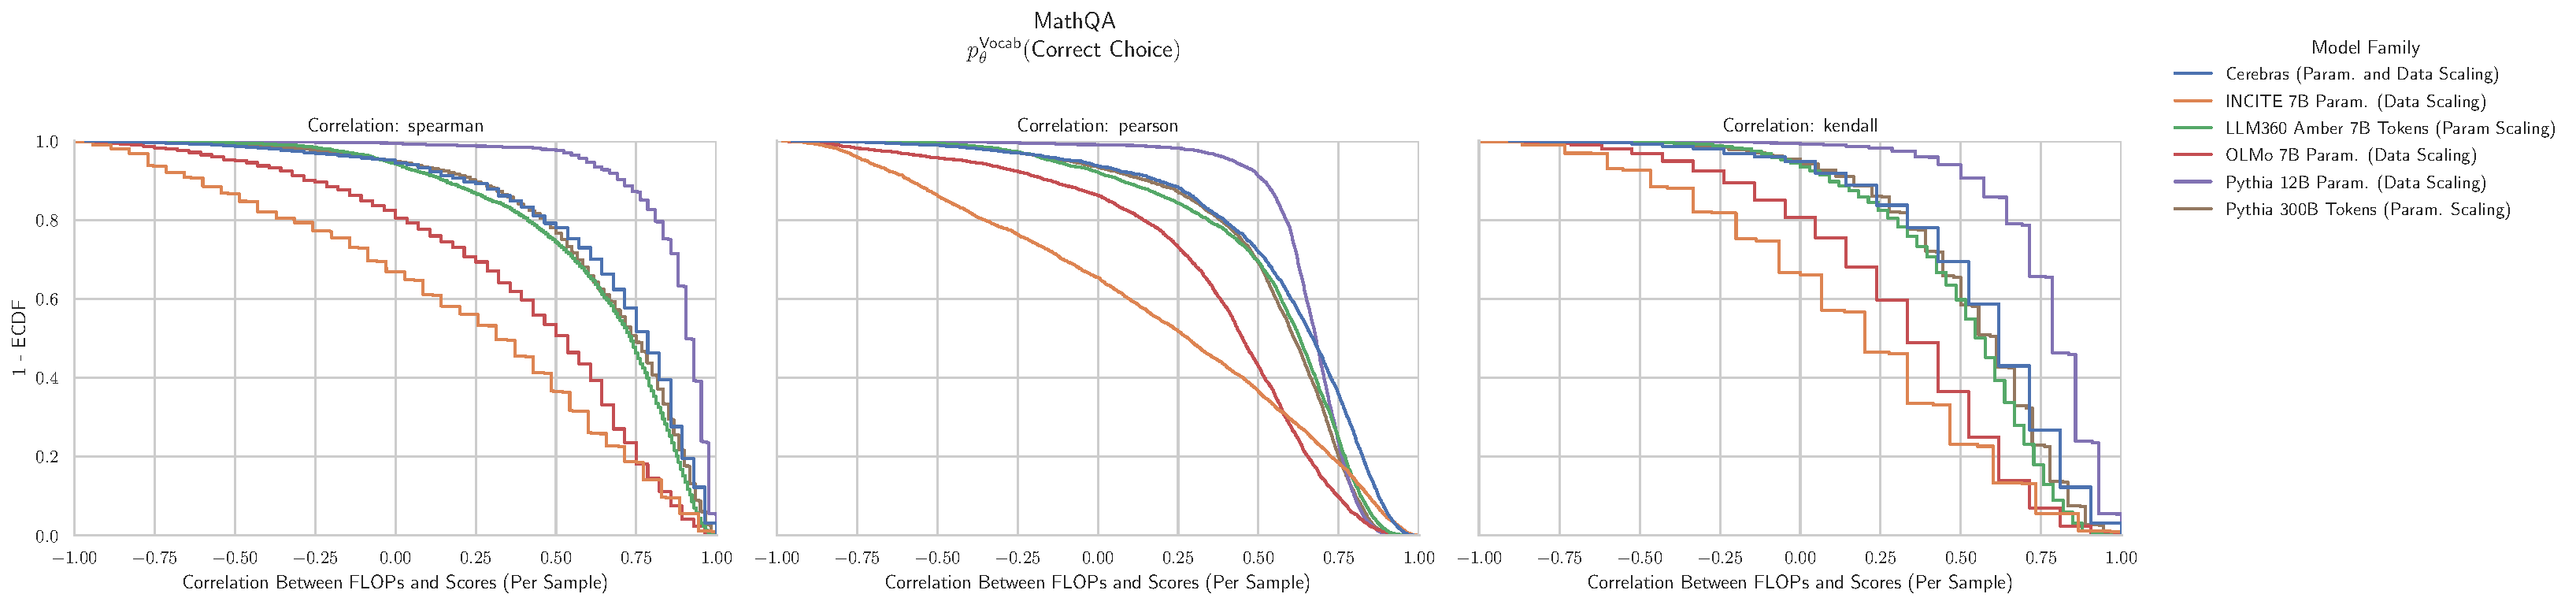
\includegraphics[width=\textwidth]{figures/correlations_between_scores_and_compute/correlation_distributions/mathqa/mathqa_prob_correct_vocab_ecdf_vs_correlation_score_by_modelfamily_split_correlation_metric.pdf}
    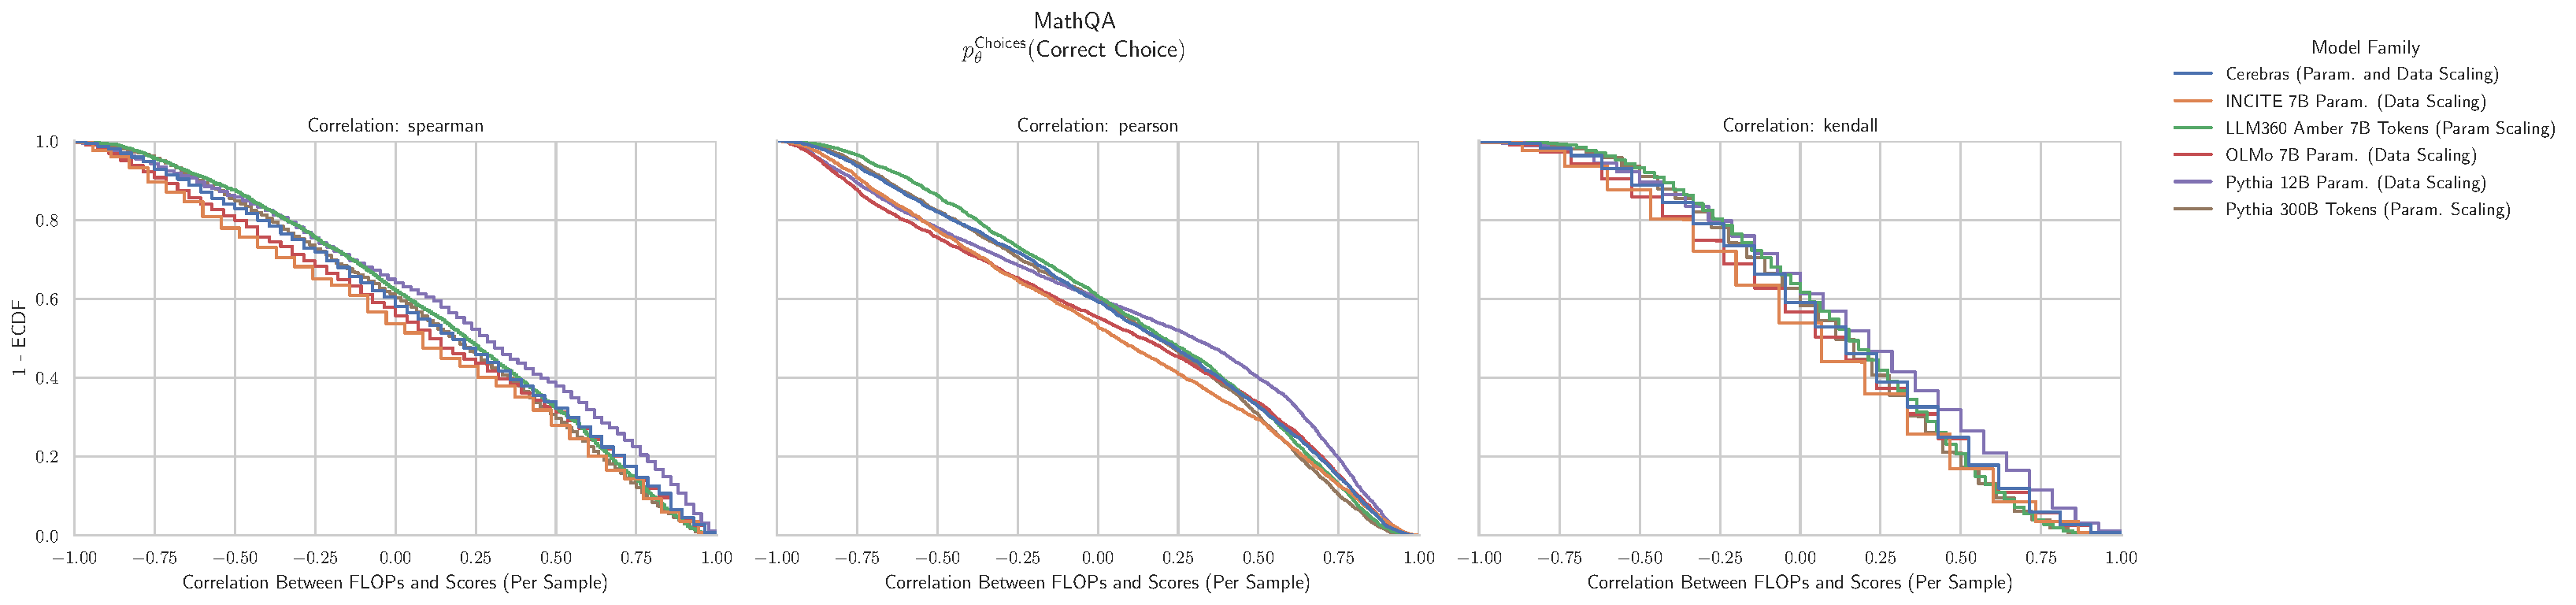
\includegraphics[width=\textwidth]{figures/correlations_between_scores_and_compute/correlation_distributions/mathqa/mathqa_prob_correct_choices_ecdf_vs_correlation_score_by_modelfamily_split_correlation_metric.pdf}
    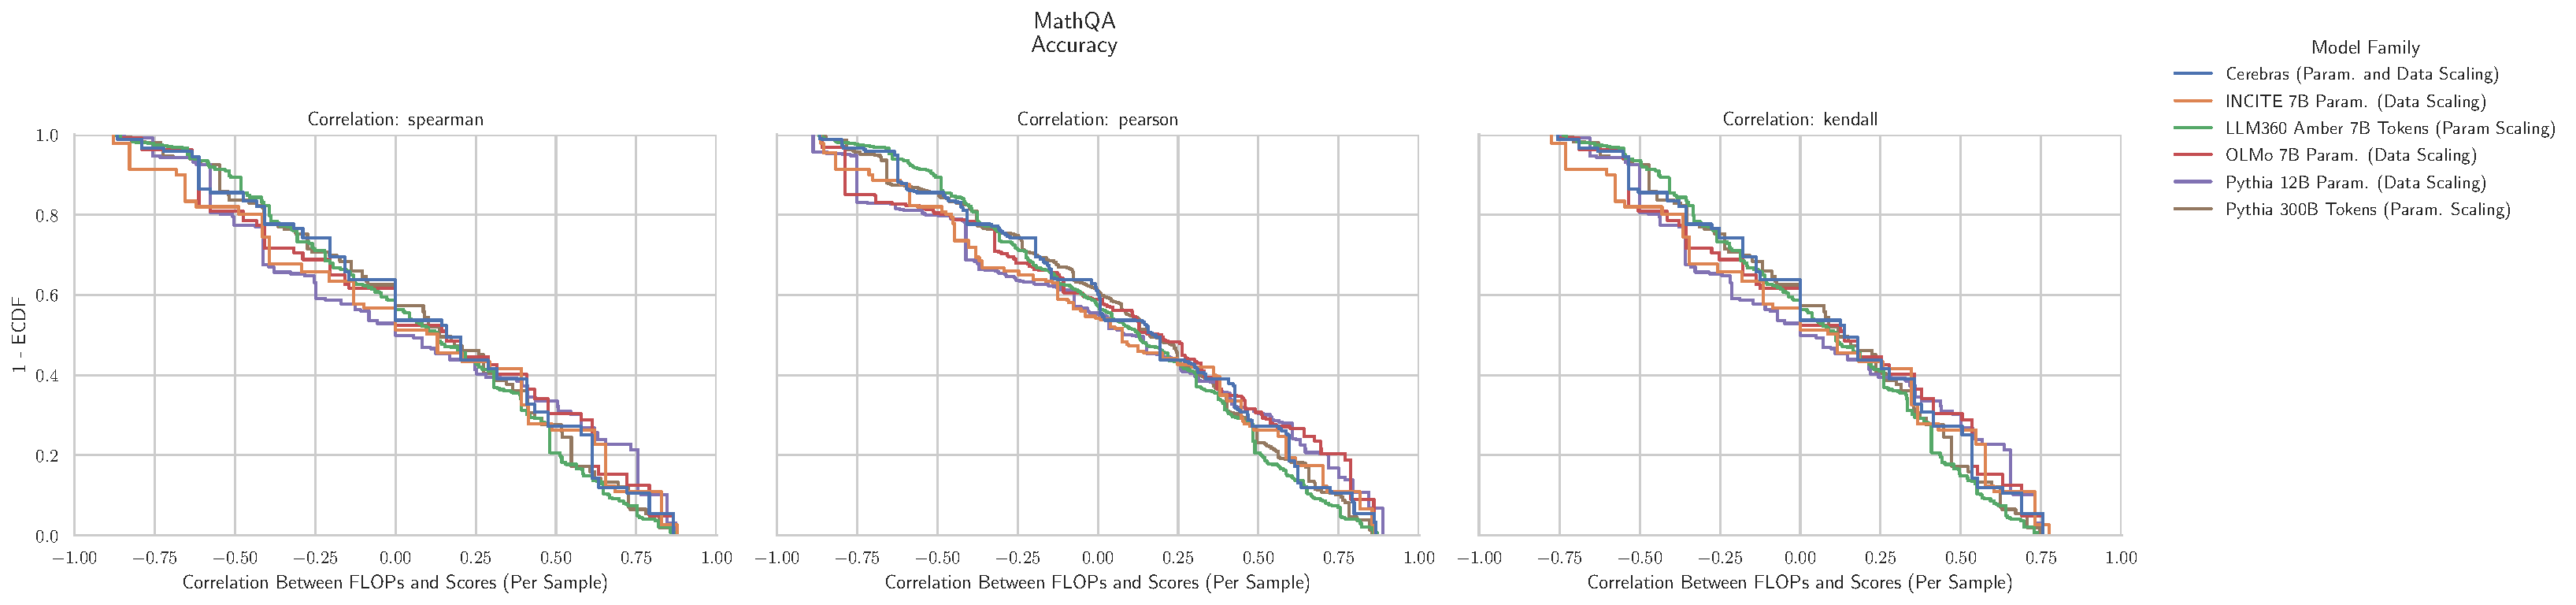
\includegraphics[width=\textwidth]{figures/correlations_between_scores_and_compute/correlation_distributions/mathqa/mathqa_acc_ecdf_vs_correlation_score_by_modelfamily_split_correlation_metric.pdf}
    \caption{\textbf{HellaSwag: Downstream performance is computed via a sequence of transformations that deteriorate correlations between scores and pretraining compute.}}
    \label{app:fig:compute_score_distribution_mathqa}
\end{figure}

\clearpage
\subsection{NLP Benchmark: MC TACO \cite{zhou2019mctaco}}

\begin{figure}[h!]
    \centering
    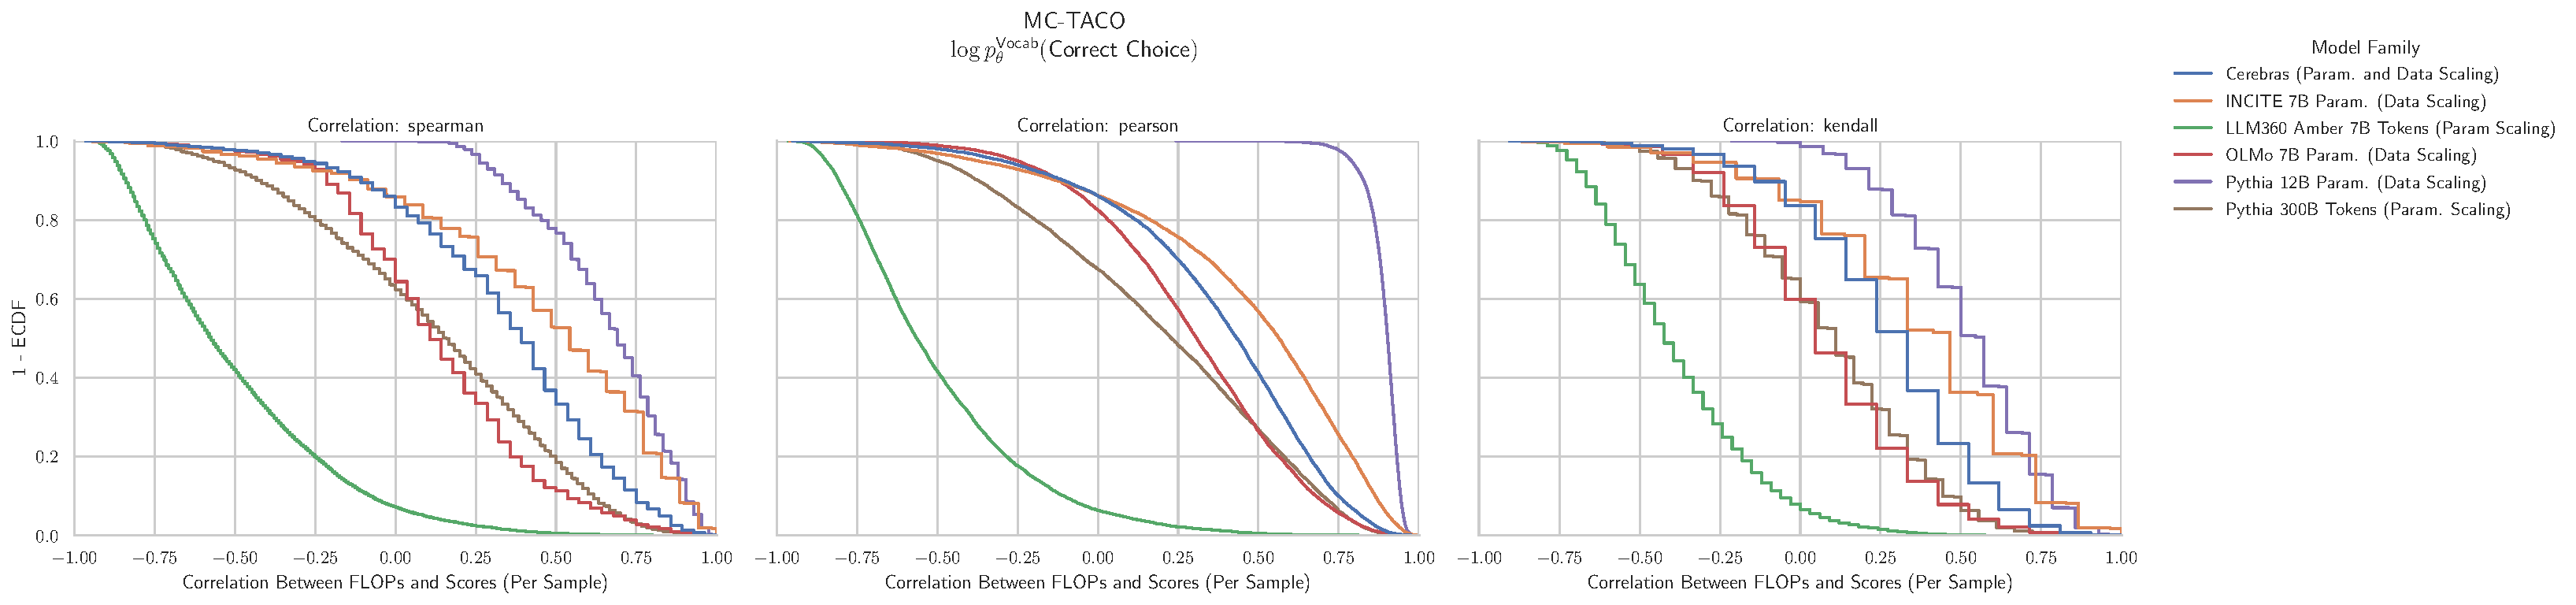
\includegraphics[width=\textwidth]{figures/correlations_between_scores_and_compute/correlation_distributions/mc_taco/mc_taco_log_likelihood_correct_ecdf_vs_correlation_score_by_modelfamily_split_correlation_metric.pdf}
    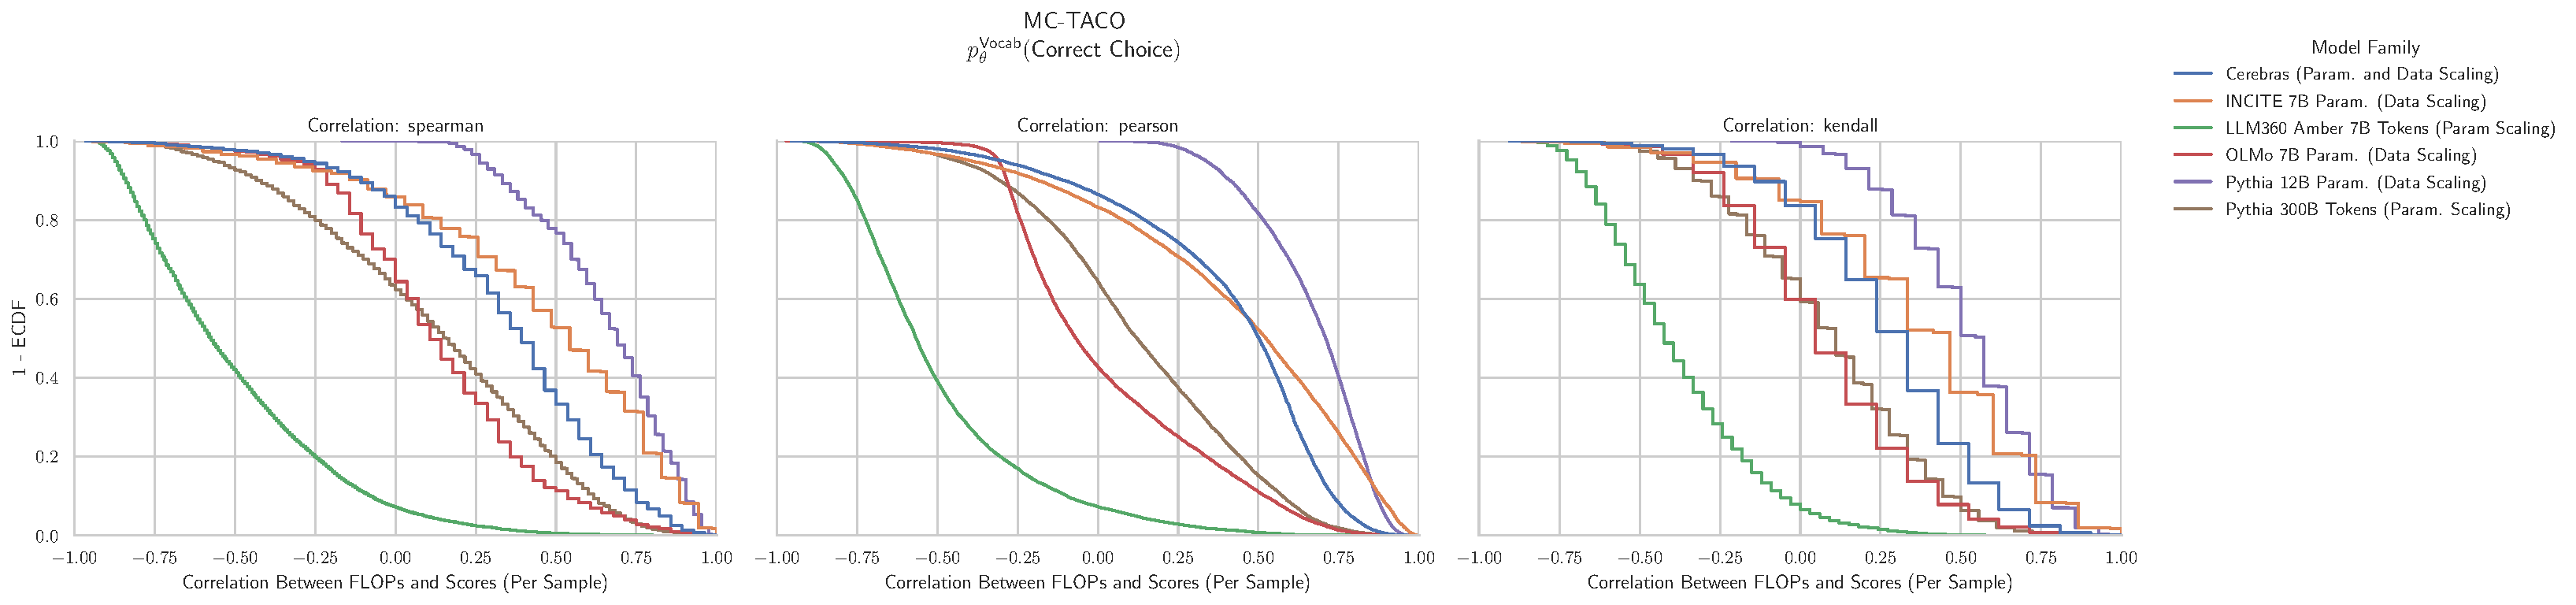
\includegraphics[width=\textwidth]{figures/correlations_between_scores_and_compute/correlation_distributions/mc_taco/mc_taco_prob_correct_vocab_ecdf_vs_correlation_score_by_modelfamily_split_correlation_metric.pdf}
    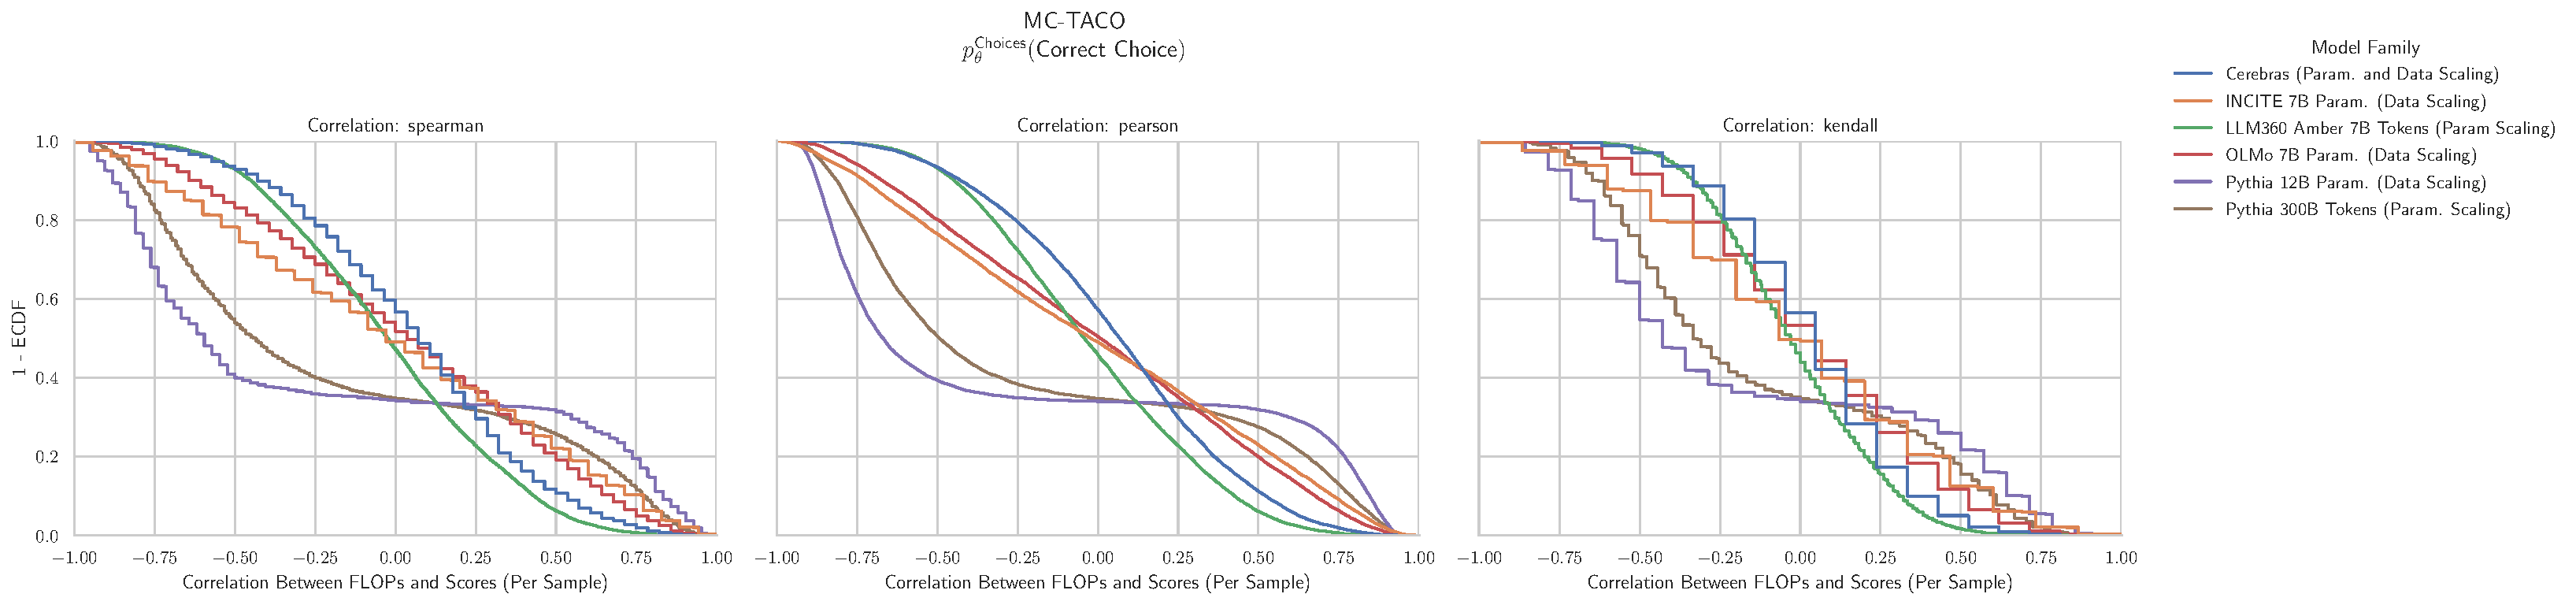
\includegraphics[width=\textwidth]{figures/correlations_between_scores_and_compute/correlation_distributions/mc_taco/mc_taco_prob_correct_choices_ecdf_vs_correlation_score_by_modelfamily_split_correlation_metric.pdf}
    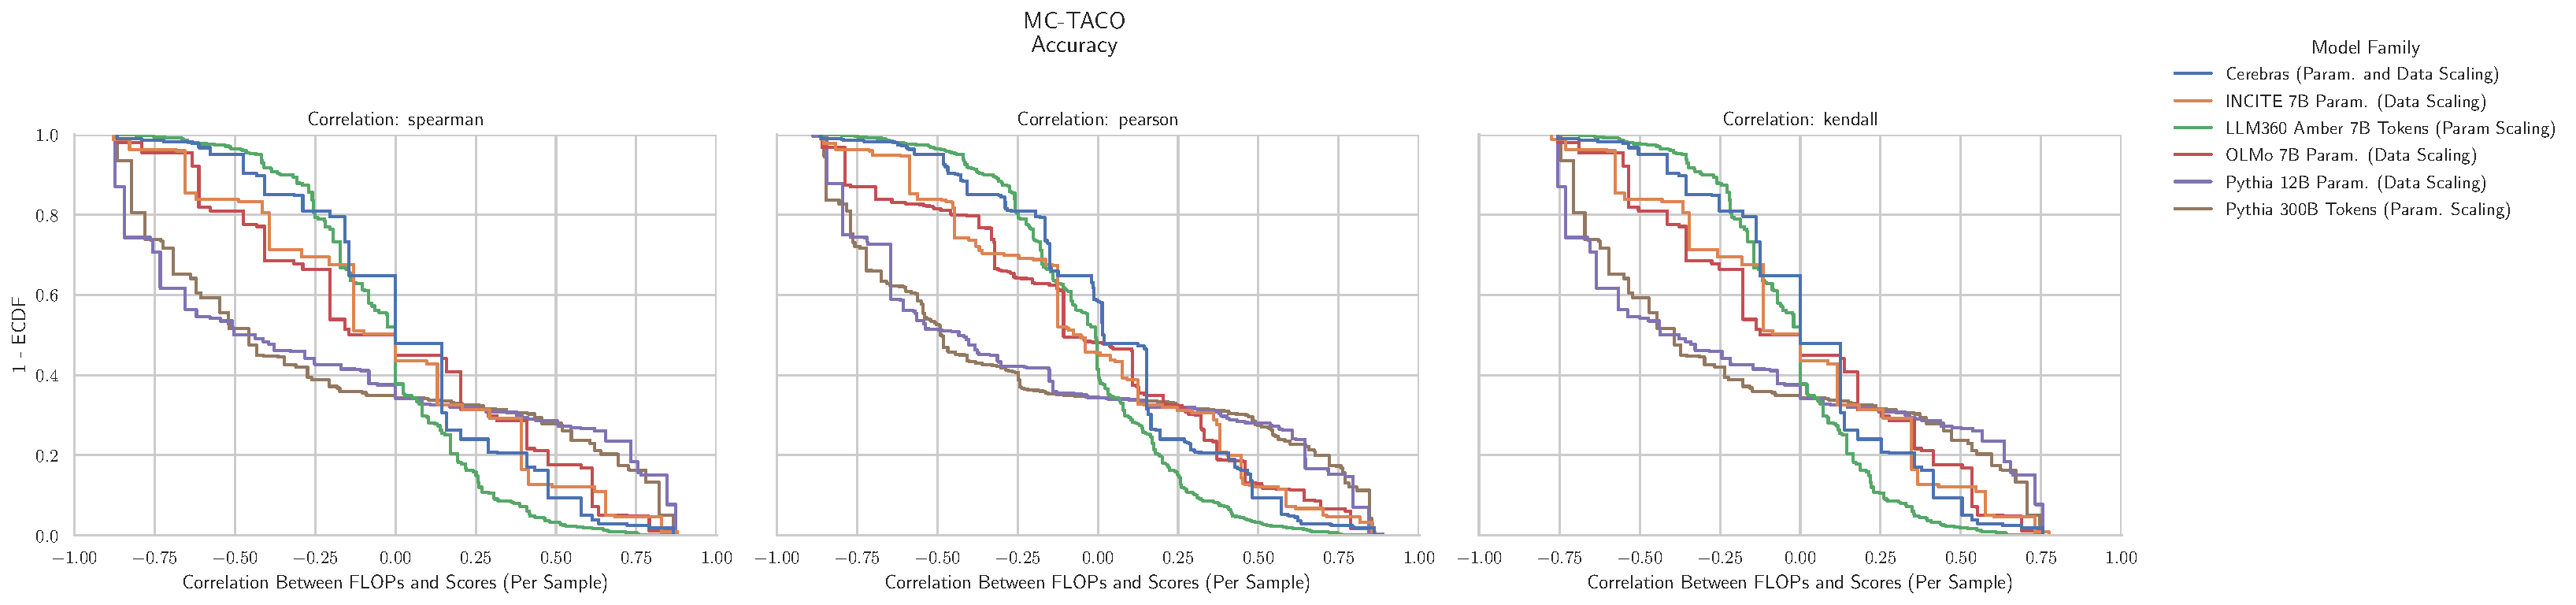
\includegraphics[width=\textwidth]{figures/correlations_between_scores_and_compute/correlation_distributions/mc_taco/mc_taco_acc_ecdf_vs_correlation_score_by_modelfamily_split_correlation_metric.pdf}
    \caption{\textbf{MC TACO: Downstream performance is computed via a sequence of transformations that deteriorate correlations between scores and pretraining compute.}}
    \label{app:fig:compute_score_distribution_mc_taco}
\end{figure}

\clearpage
\subsection{NLP Benchmark: MMLU Abstract Algebra \cite{hendrycks2020mmlu}}

\begin{figure}[h!]
    \centering
    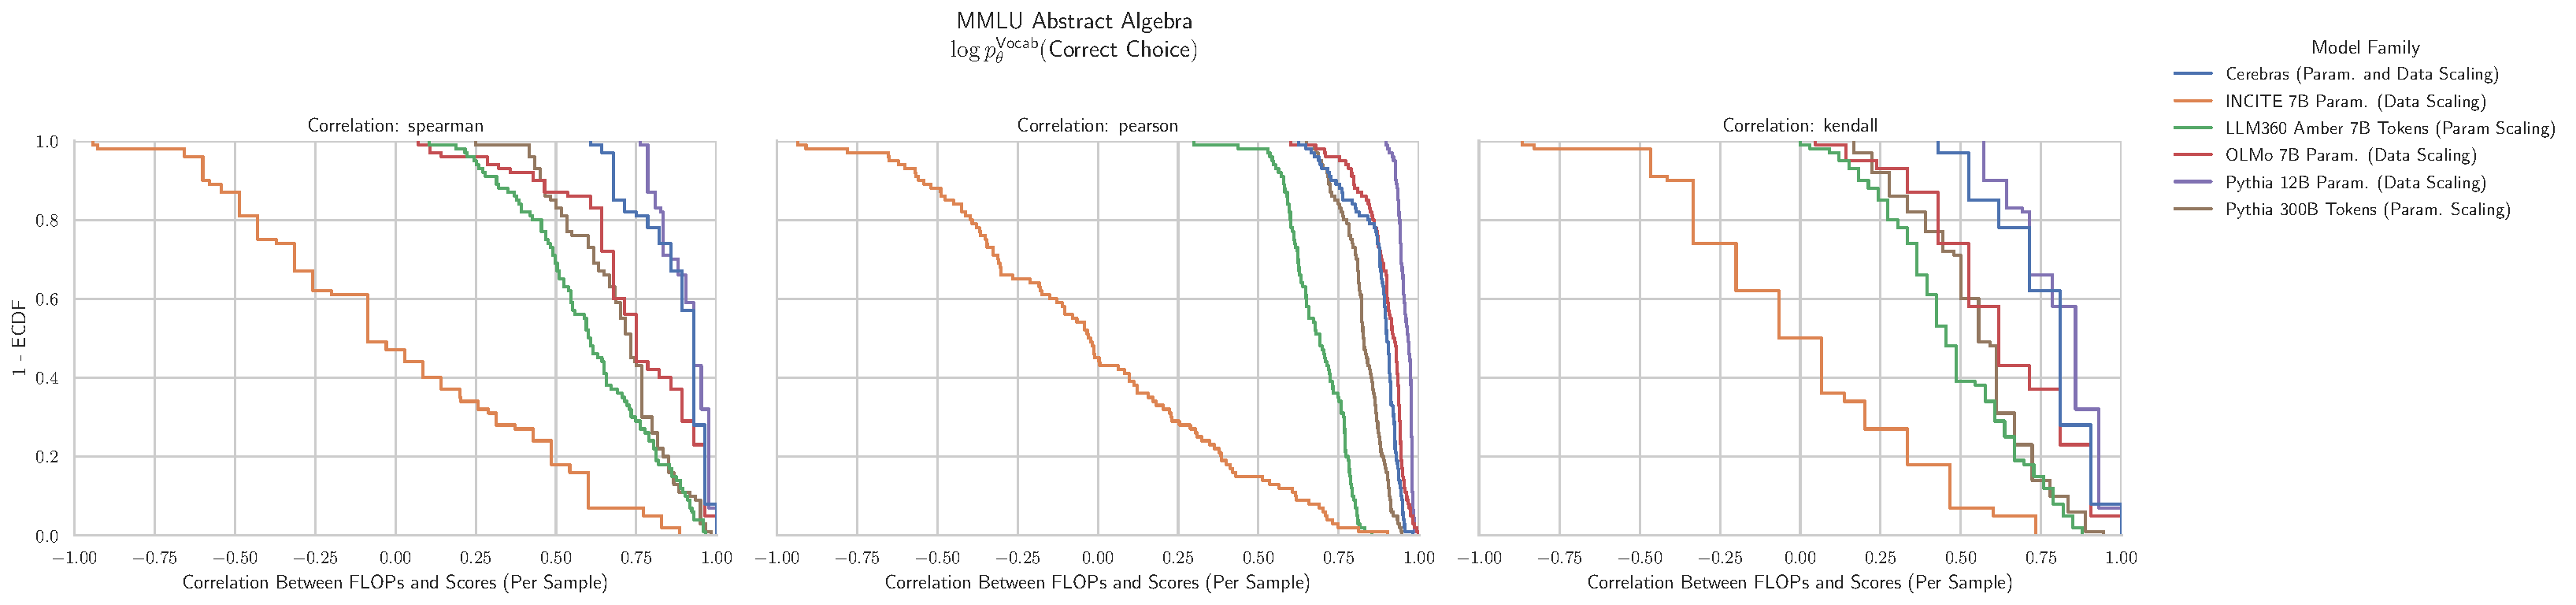
\includegraphics[width=\textwidth]{figures/correlations_between_scores_and_compute/correlation_distributions/mmlu_abstract_algebra/mmlu_abstract_algebra_log_likelihood_correct_ecdf_vs_correlation_score_by_modelfamily_split_correlation_metric.pdf}
    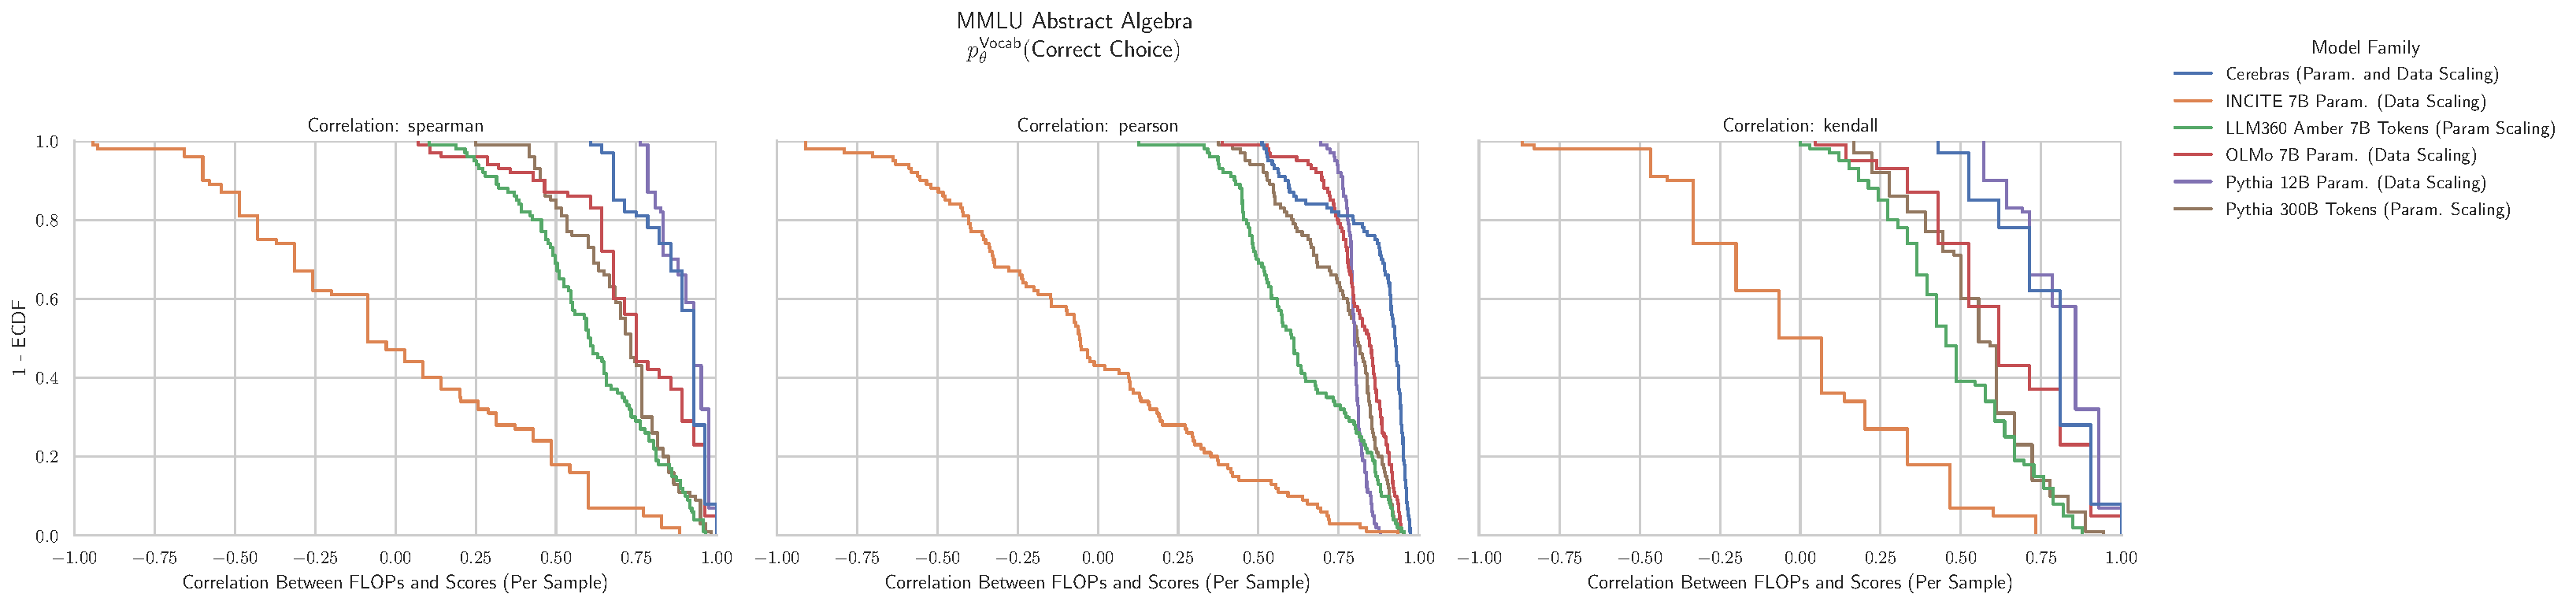
\includegraphics[width=\textwidth]{figures/correlations_between_scores_and_compute/correlation_distributions/mmlu_abstract_algebra/mmlu_abstract_algebra_prob_correct_vocab_ecdf_vs_correlation_score_by_modelfamily_split_correlation_metric.pdf}
    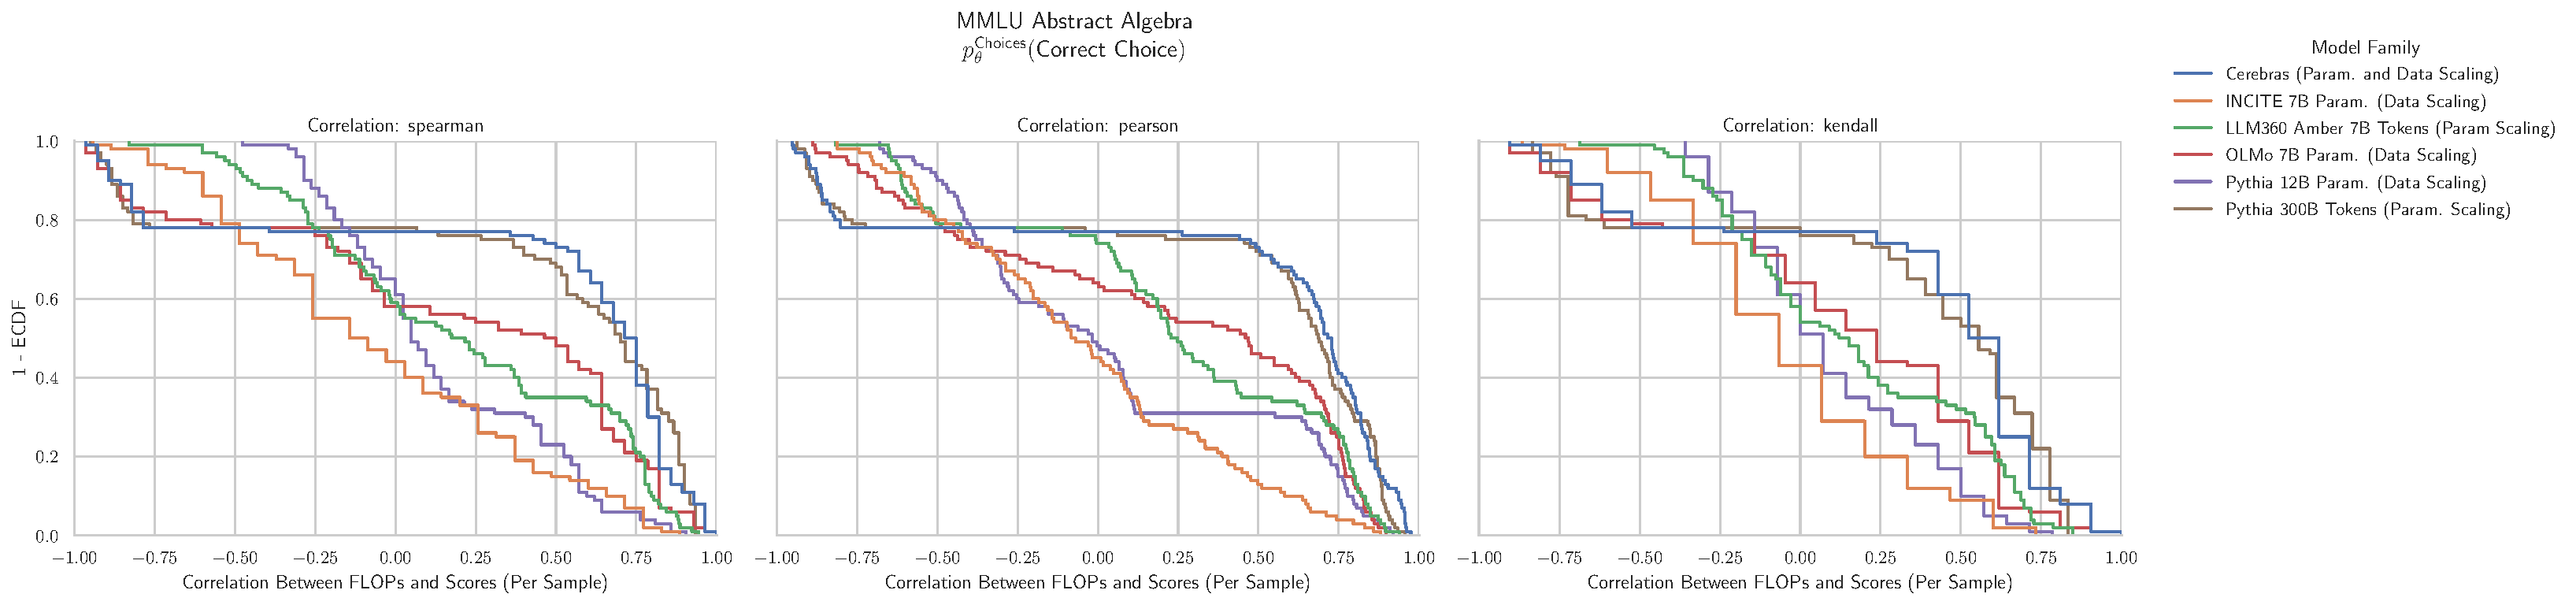
\includegraphics[width=\textwidth]{figures/correlations_between_scores_and_compute/correlation_distributions/mmlu_abstract_algebra/mmlu_abstract_algebra_prob_correct_choices_ecdf_vs_correlation_score_by_modelfamily_split_correlation_metric.pdf}
    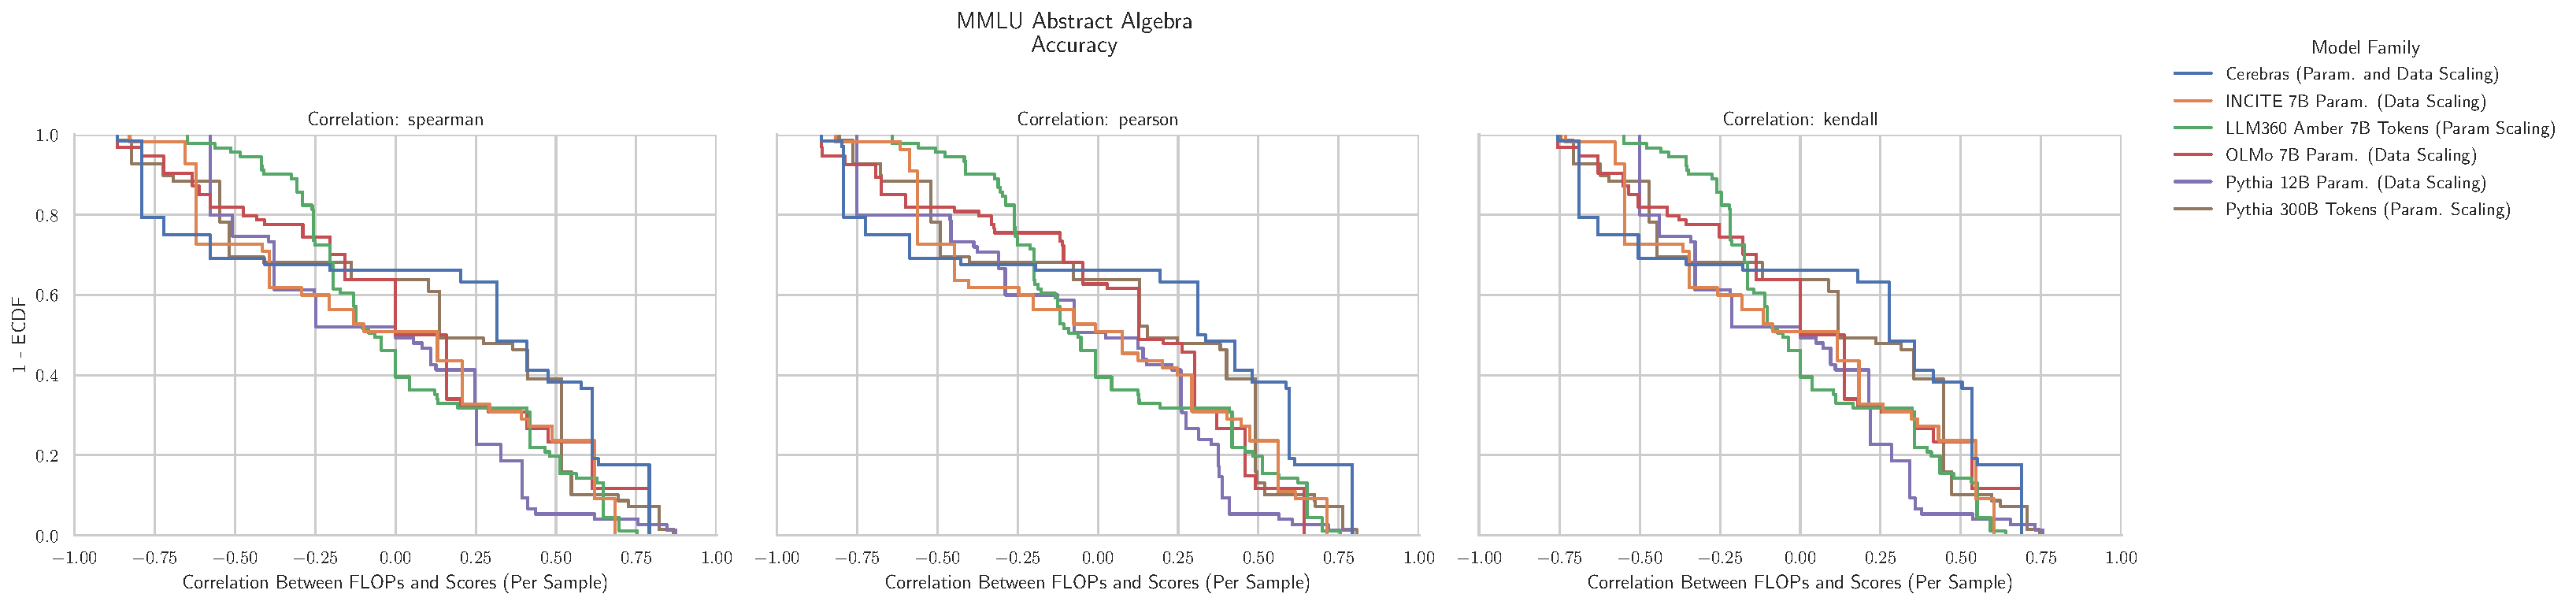
\includegraphics[width=\textwidth]{figures/correlations_between_scores_and_compute/correlation_distributions/mmlu_abstract_algebra/mmlu_abstract_algebra_acc_ecdf_vs_correlation_score_by_modelfamily_split_correlation_metric.pdf}
    \caption{\textbf{MMLU Abstract Algebra: Downstream performance is computed via a sequence of transformations that deteriorate correlations between scores and pretraining compute.}}
    \label{app:fig:compute_score_distribution_mmlu_abstract_algebra}
\end{figure}

\clearpage
\subsection{NLP Benchmark: MMLU Anatomy \cite{hendrycks2020mmlu}}

\begin{figure}[h!]
    \centering
    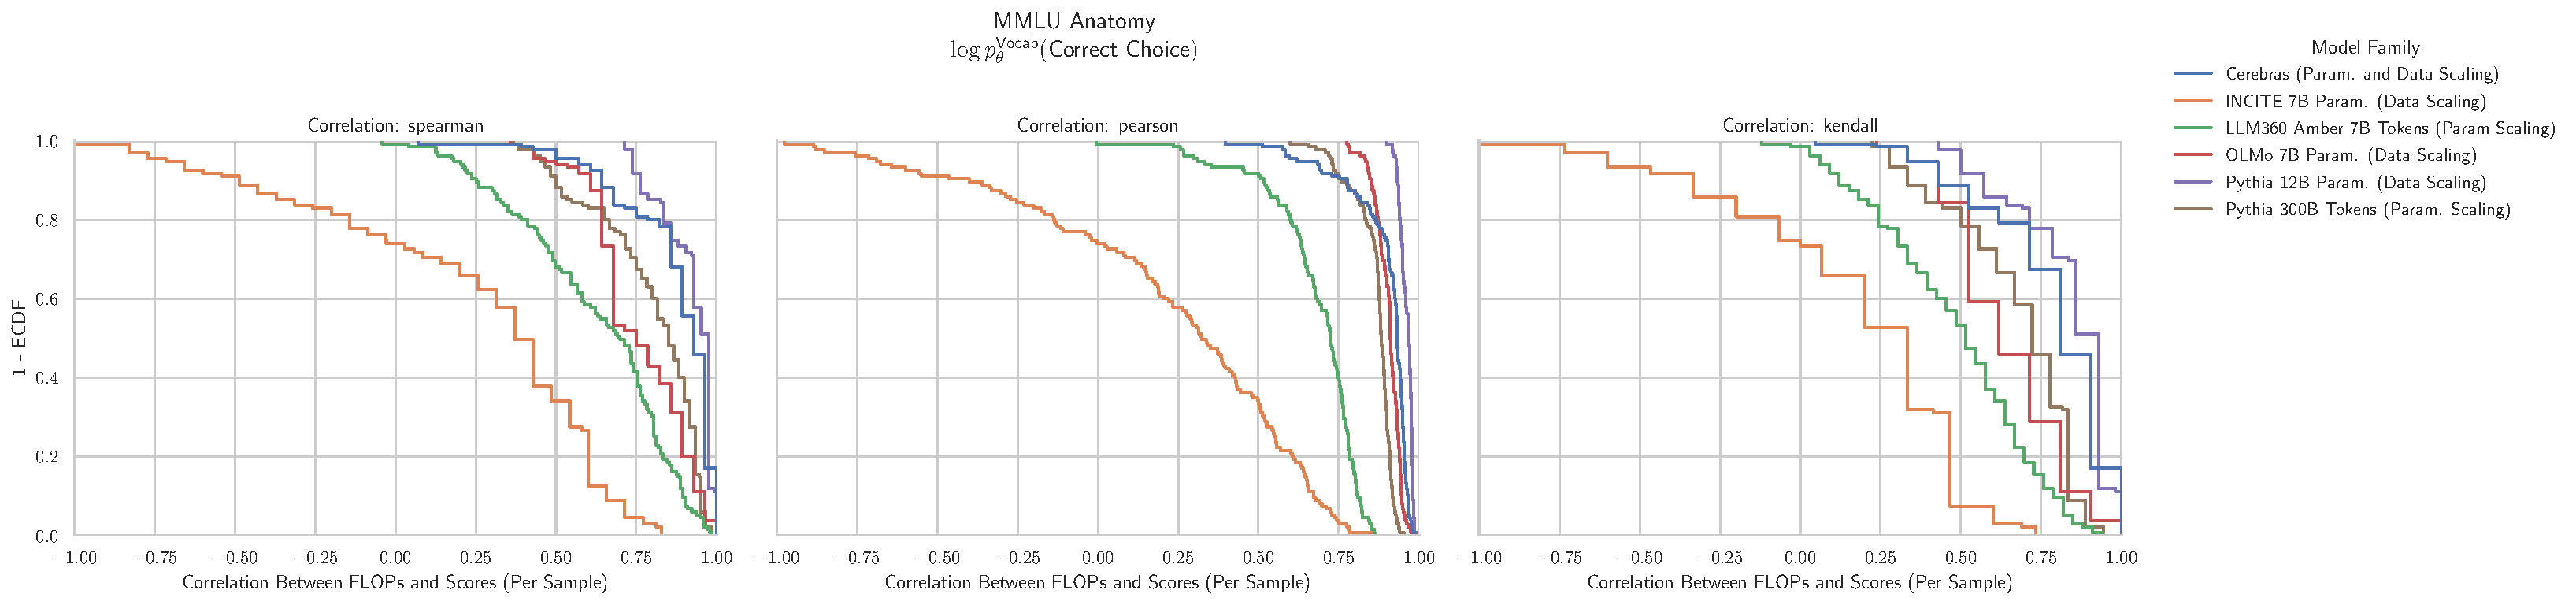
\includegraphics[width=\textwidth]{figures/correlations_between_scores_and_compute/correlation_distributions/mmlu_anatomy/mmlu_anatomy_log_likelihood_correct_ecdf_vs_correlation_score_by_modelfamily_split_correlation_metric.pdf}
    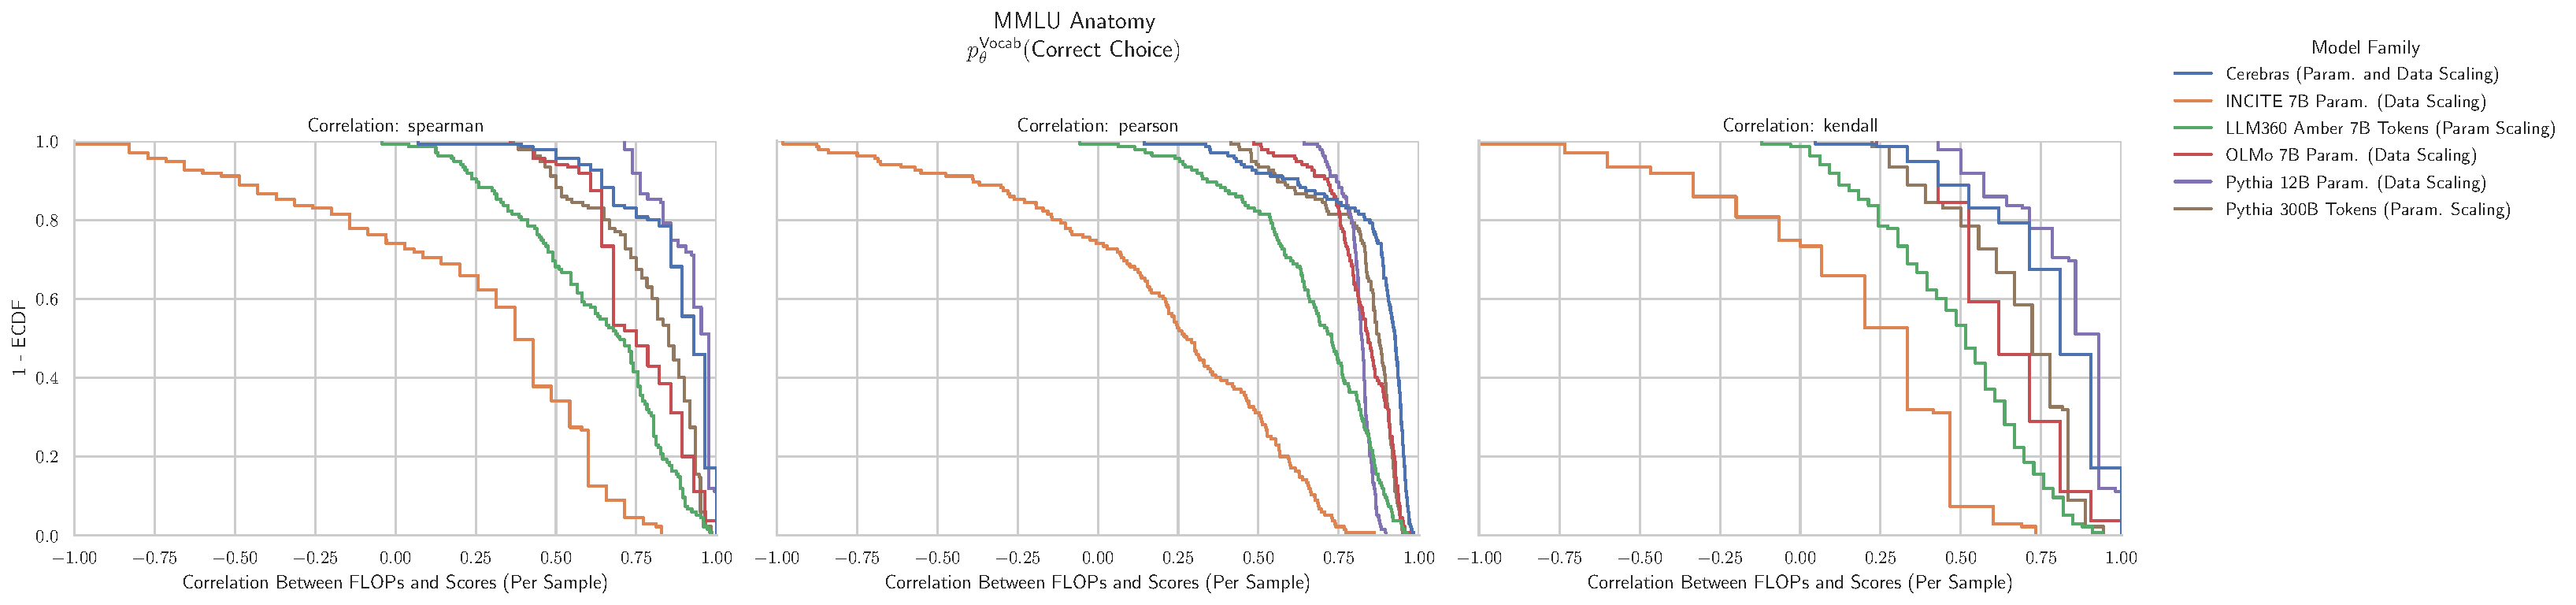
\includegraphics[width=\textwidth]{figures/correlations_between_scores_and_compute/correlation_distributions/mmlu_anatomy/mmlu_anatomy_prob_correct_vocab_ecdf_vs_correlation_score_by_modelfamily_split_correlation_metric.pdf}
    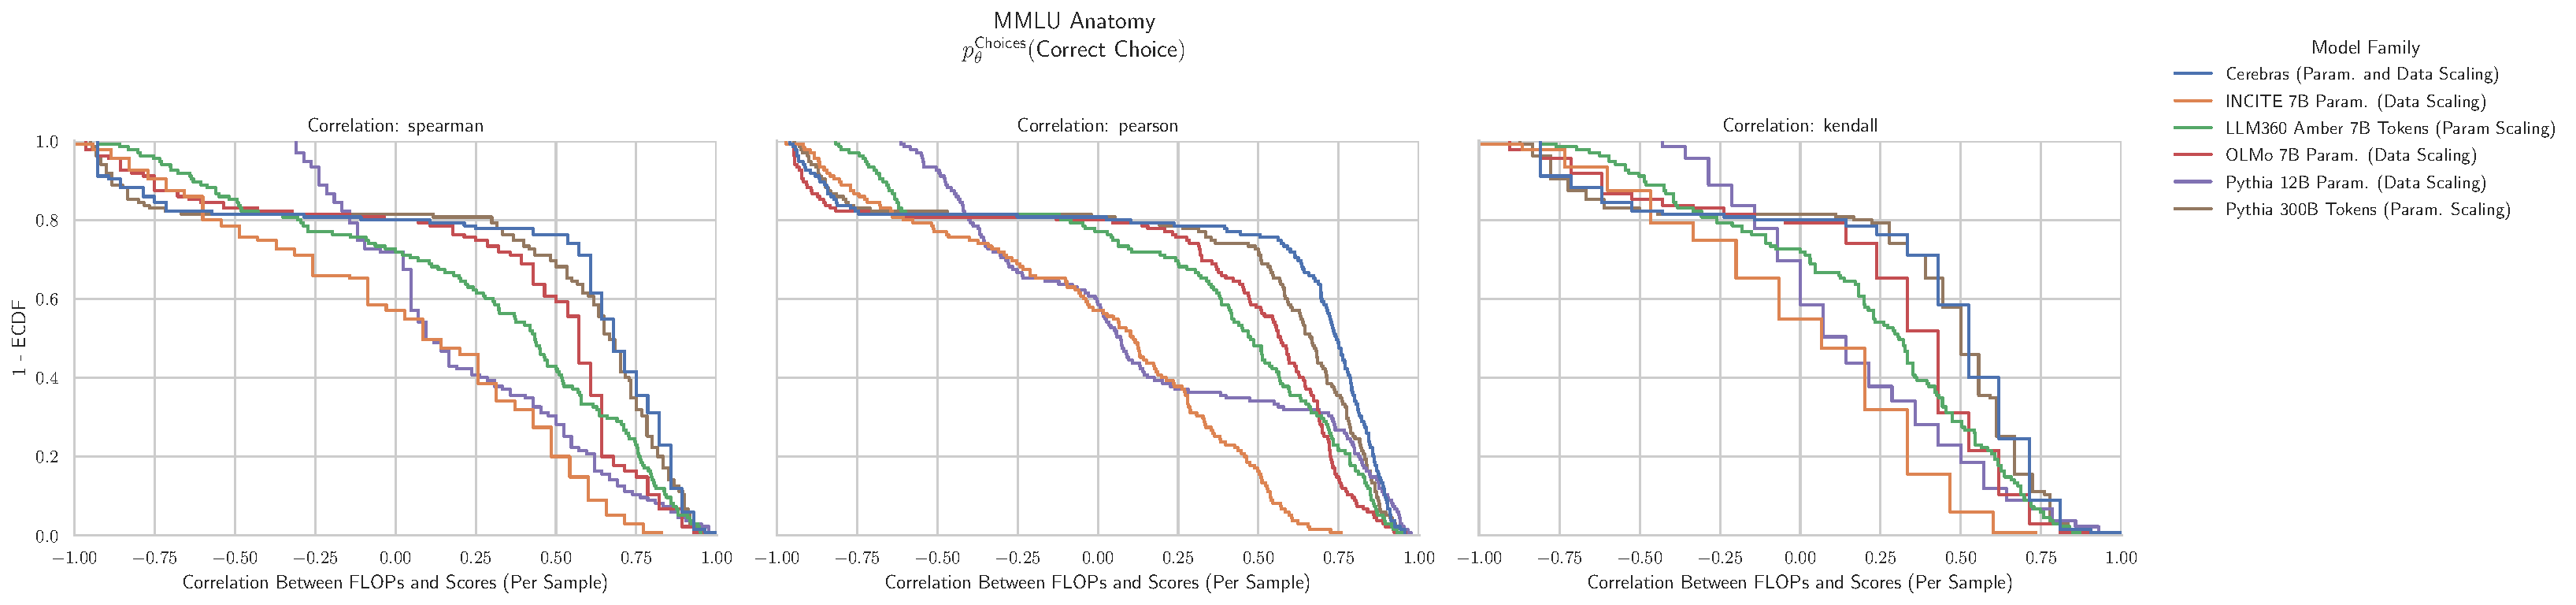
\includegraphics[width=\textwidth]{figures/correlations_between_scores_and_compute/correlation_distributions/mmlu_anatomy/mmlu_anatomy_prob_correct_choices_ecdf_vs_correlation_score_by_modelfamily_split_correlation_metric.pdf}
    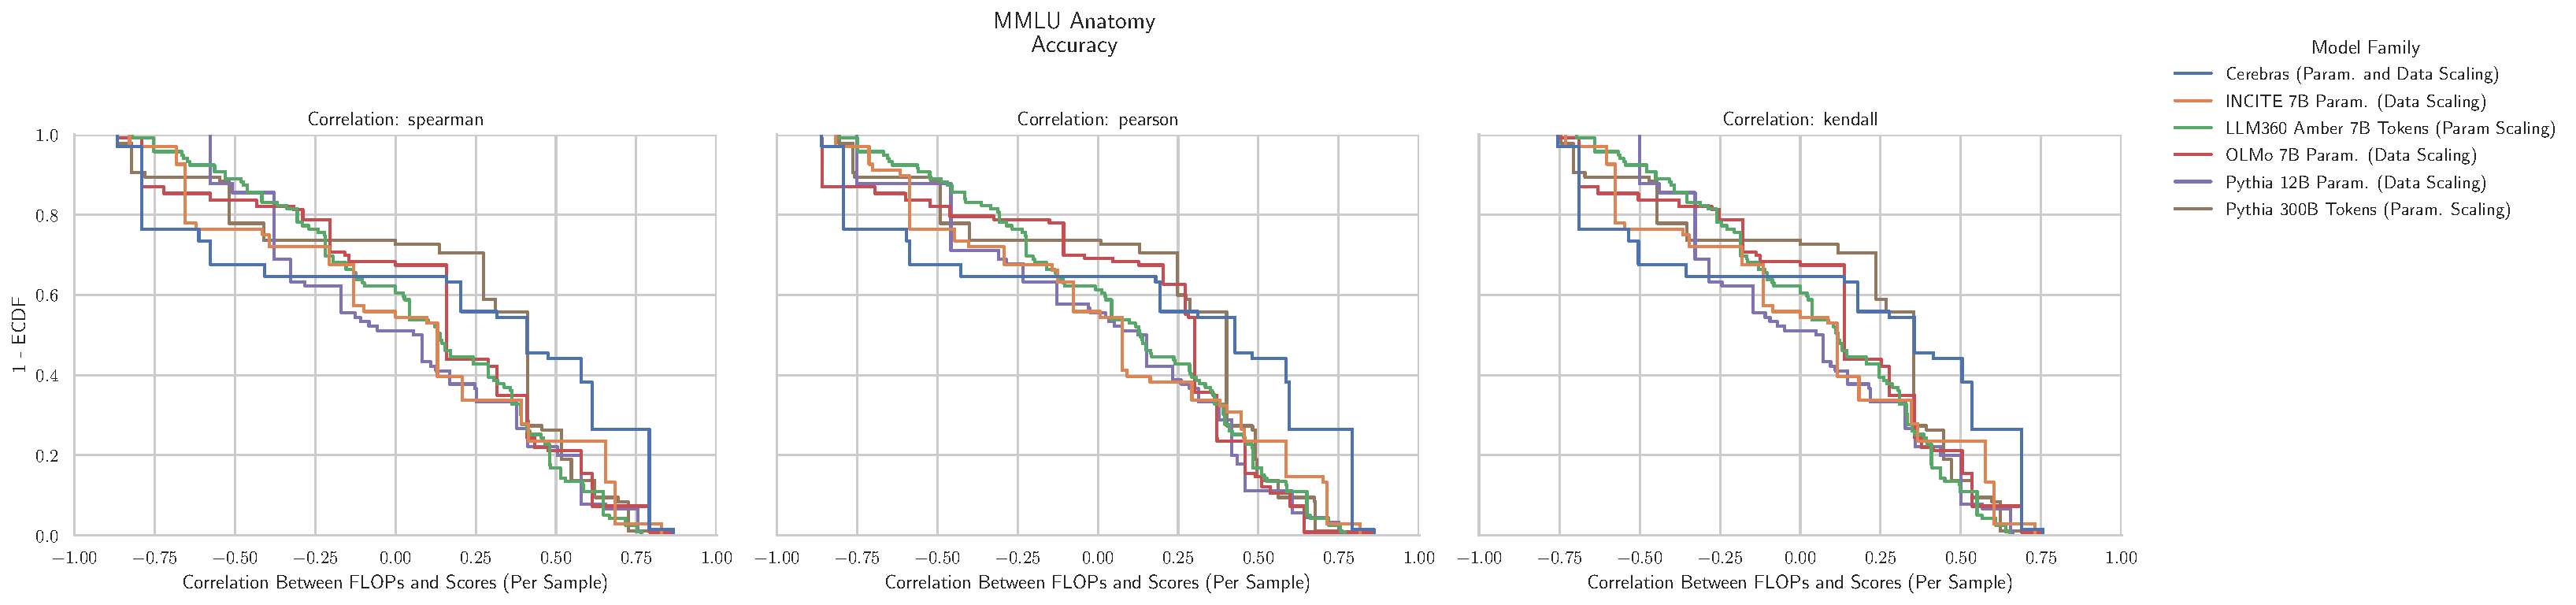
\includegraphics[width=\textwidth]{figures/correlations_between_scores_and_compute/correlation_distributions/mmlu_anatomy/mmlu_anatomy_acc_ecdf_vs_correlation_score_by_modelfamily_split_correlation_metric.pdf}
    \caption{\textbf{MMLU Anatomy: Downstream performance is computed via a sequence of transformations that deteriorate correlations between scores and pretraining compute.}}
    \label{app:fig:compute_score_distribution_mmlu_anatomy}
\end{figure}

\clearpage
\subsection{NLP Benchmark: MMLU Astronomy \cite{hendrycks2020mmlu}}

\begin{figure}[h!]
    \centering
    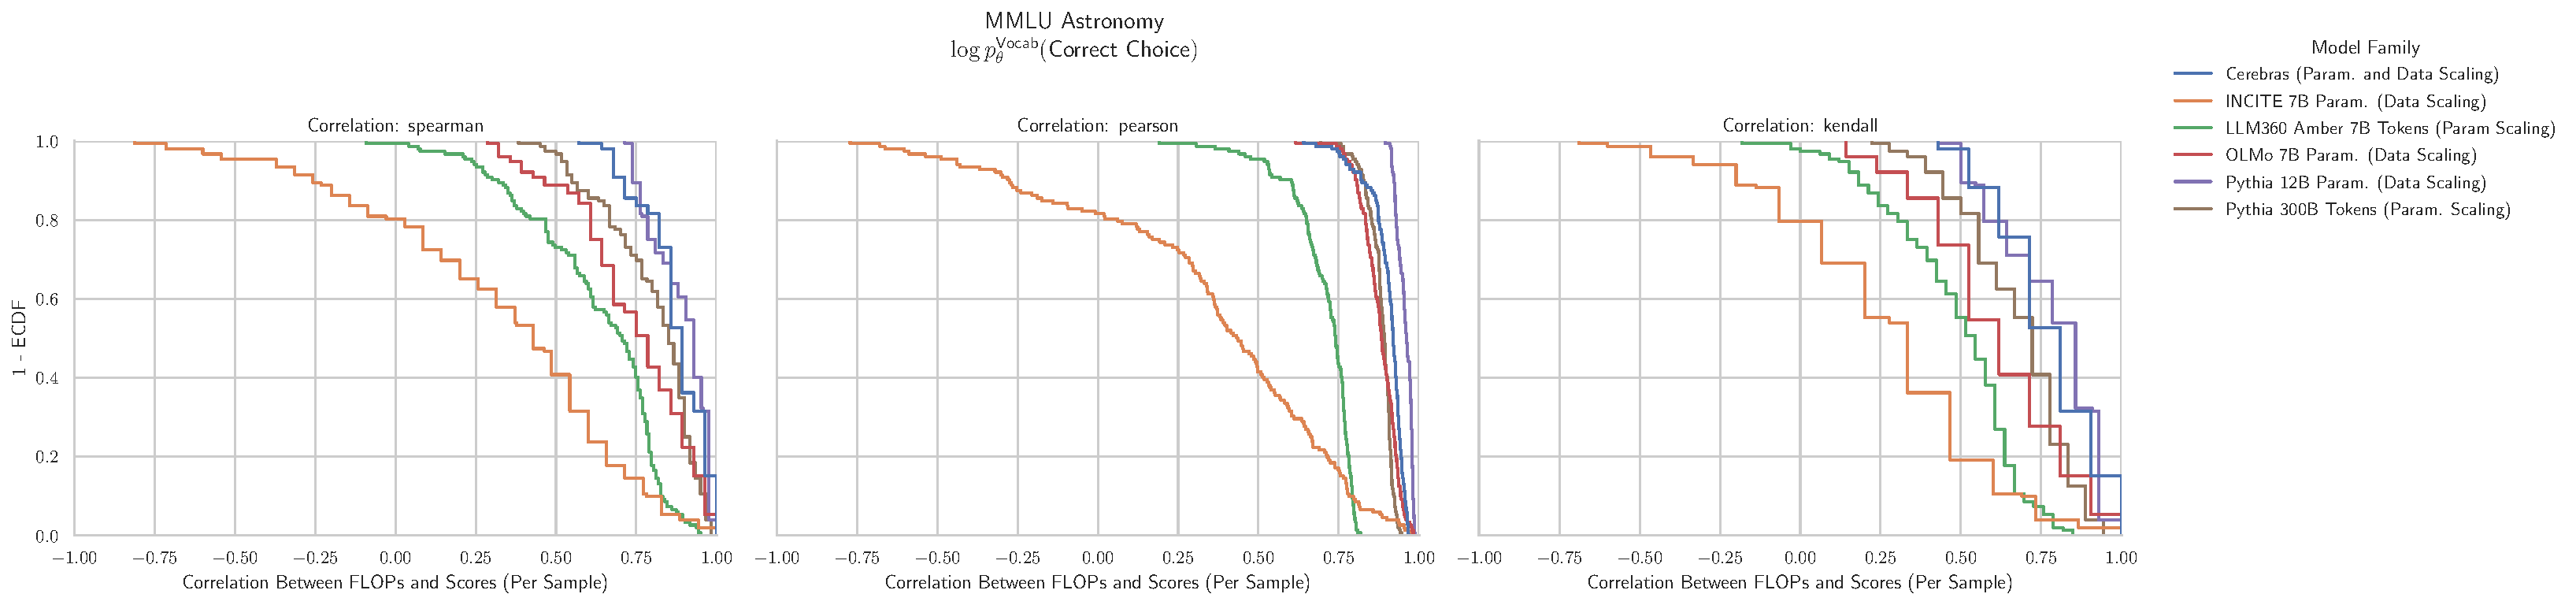
\includegraphics[width=\textwidth]{figures/correlations_between_scores_and_compute/correlation_distributions/mmlu_astronomy/mmlu_astronomy_log_likelihood_correct_ecdf_vs_correlation_score_by_modelfamily_split_correlation_metric.pdf}
    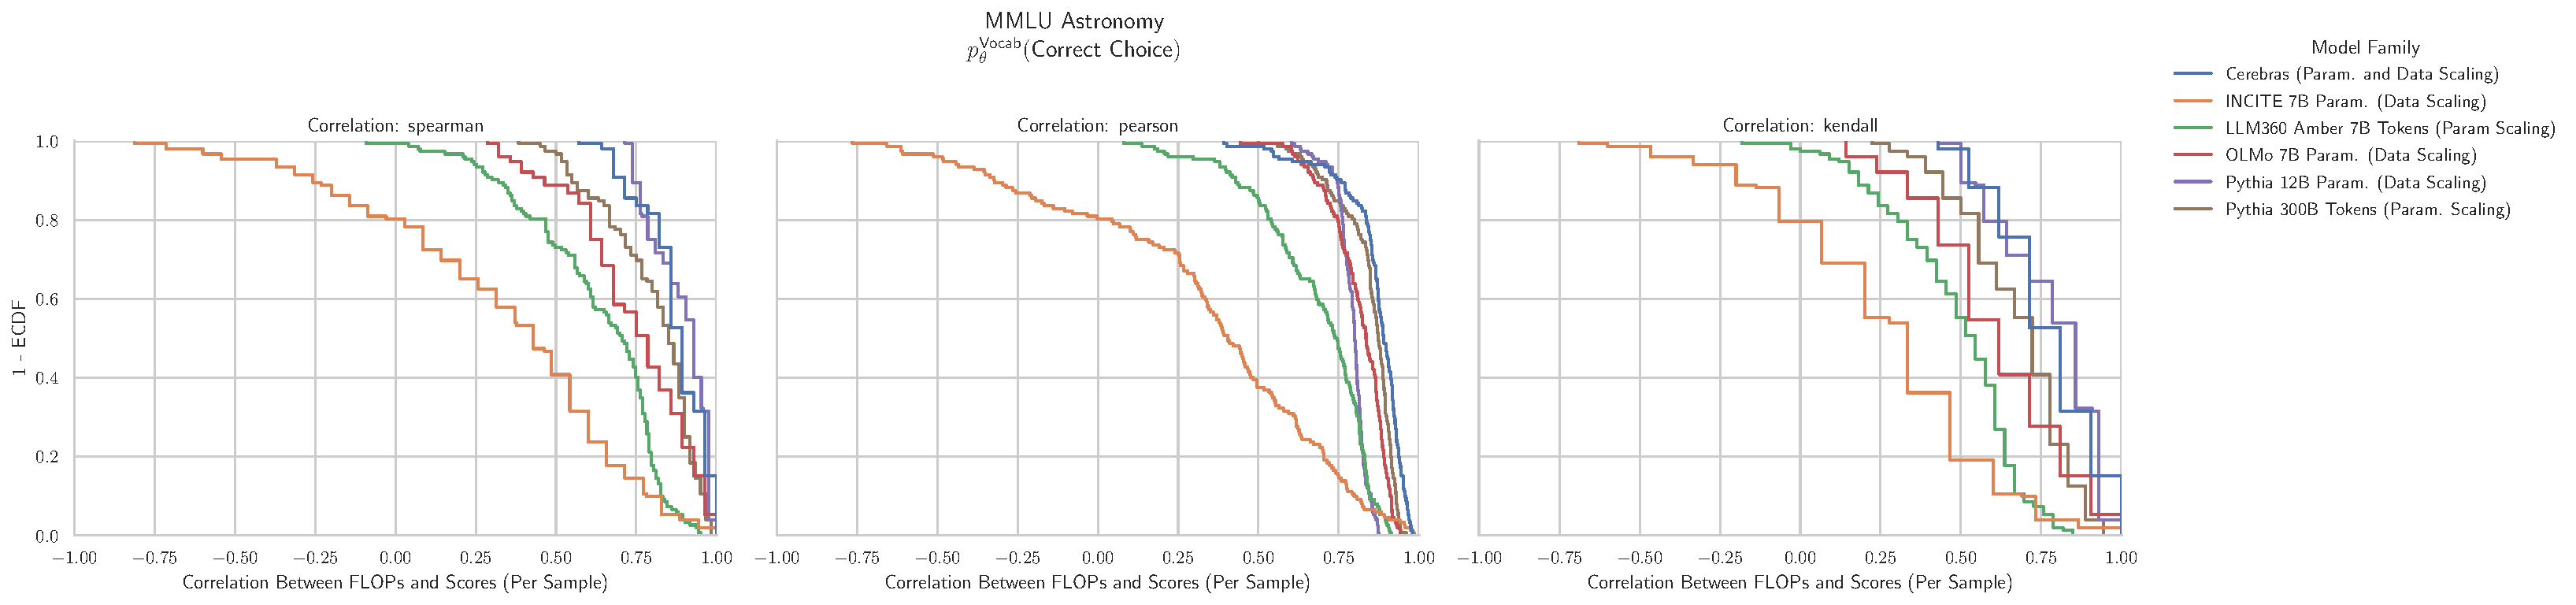
\includegraphics[width=\textwidth]{figures/correlations_between_scores_and_compute/correlation_distributions/mmlu_astronomy/mmlu_astronomy_prob_correct_vocab_ecdf_vs_correlation_score_by_modelfamily_split_correlation_metric.pdf}
    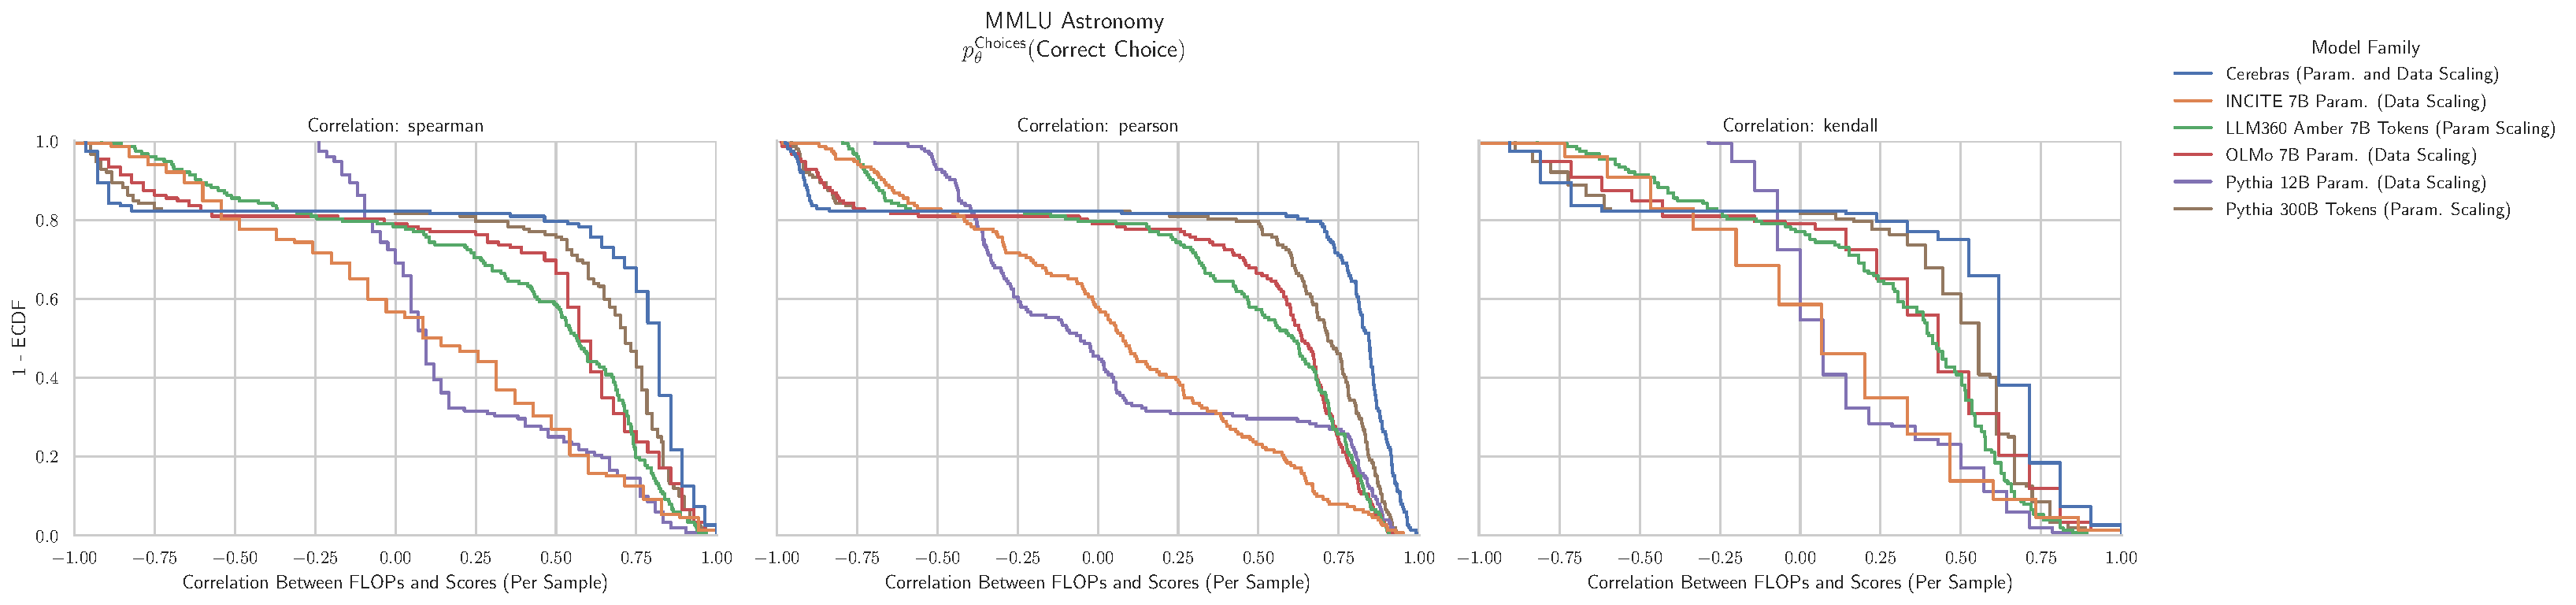
\includegraphics[width=\textwidth]{figures/correlations_between_scores_and_compute/correlation_distributions/mmlu_astronomy/mmlu_astronomy_prob_correct_choices_ecdf_vs_correlation_score_by_modelfamily_split_correlation_metric.pdf}
    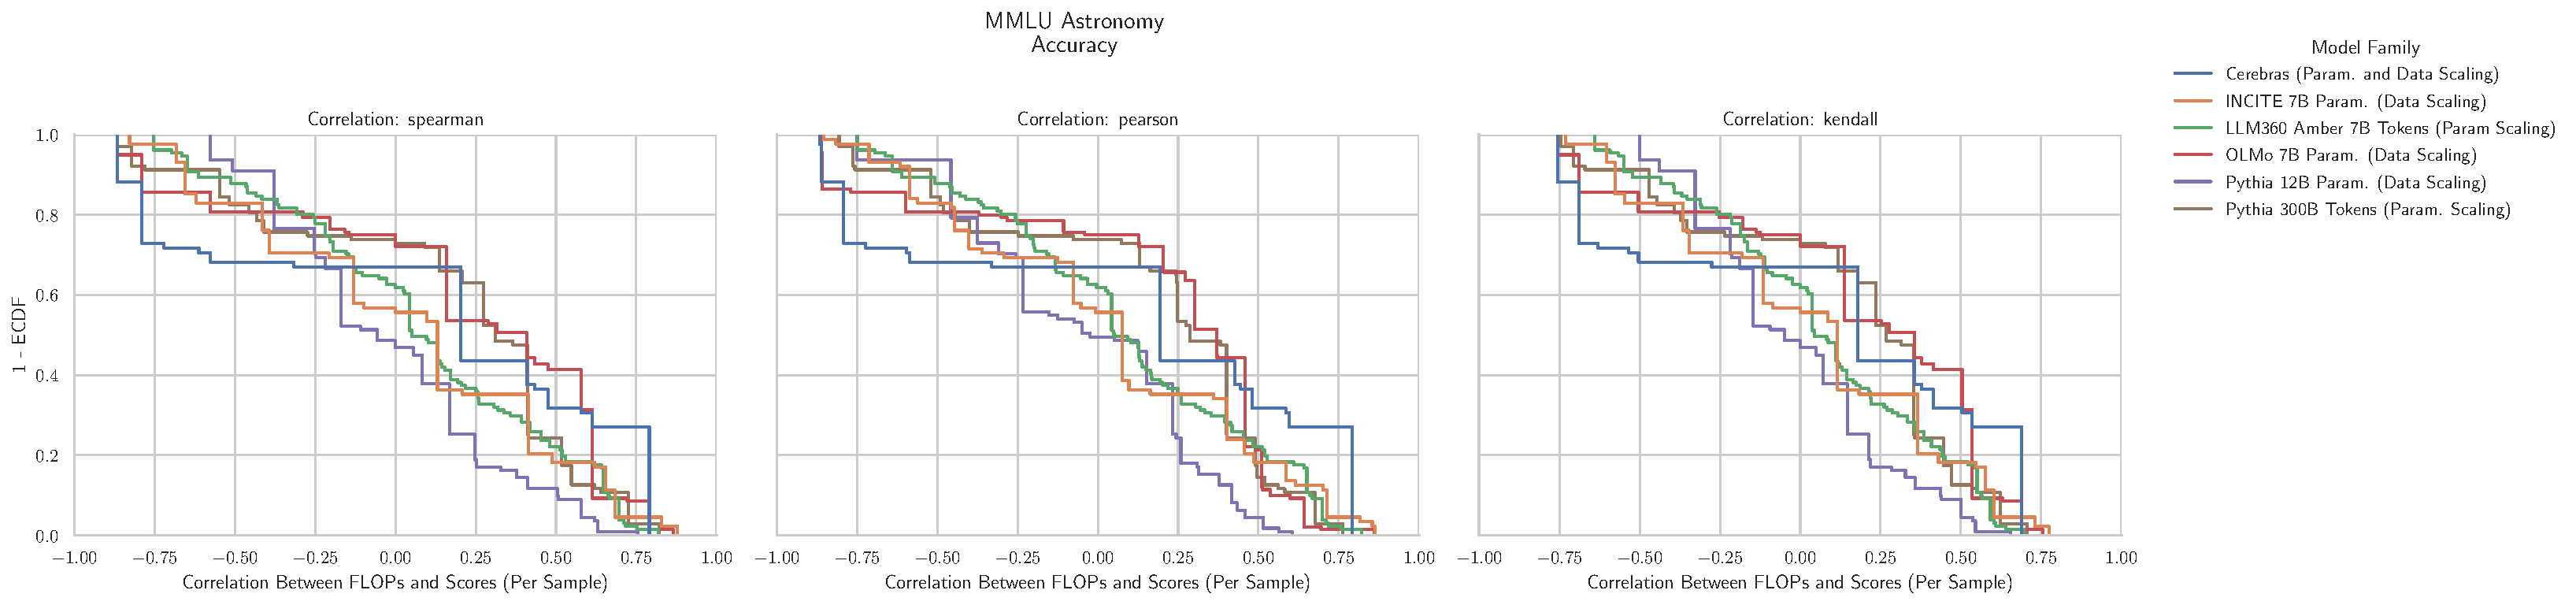
\includegraphics[width=\textwidth]{figures/correlations_between_scores_and_compute/correlation_distributions/mmlu_astronomy/mmlu_astronomy_acc_ecdf_vs_correlation_score_by_modelfamily_split_correlation_metric.pdf}
    \caption{\textbf{MMLU Astronomy: Downstream performance is computed via a sequence of transformations that deteriorate correlations between scores and pretraining compute.}}
    \label{app:fig:compute_score_distribution_mmlu_astronomy}
\end{figure}

\clearpage
\subsection{NLP Benchmark: MMLU Business Ethics \cite{hendrycks2020mmlu}}

\begin{figure}[h!]
    \centering
    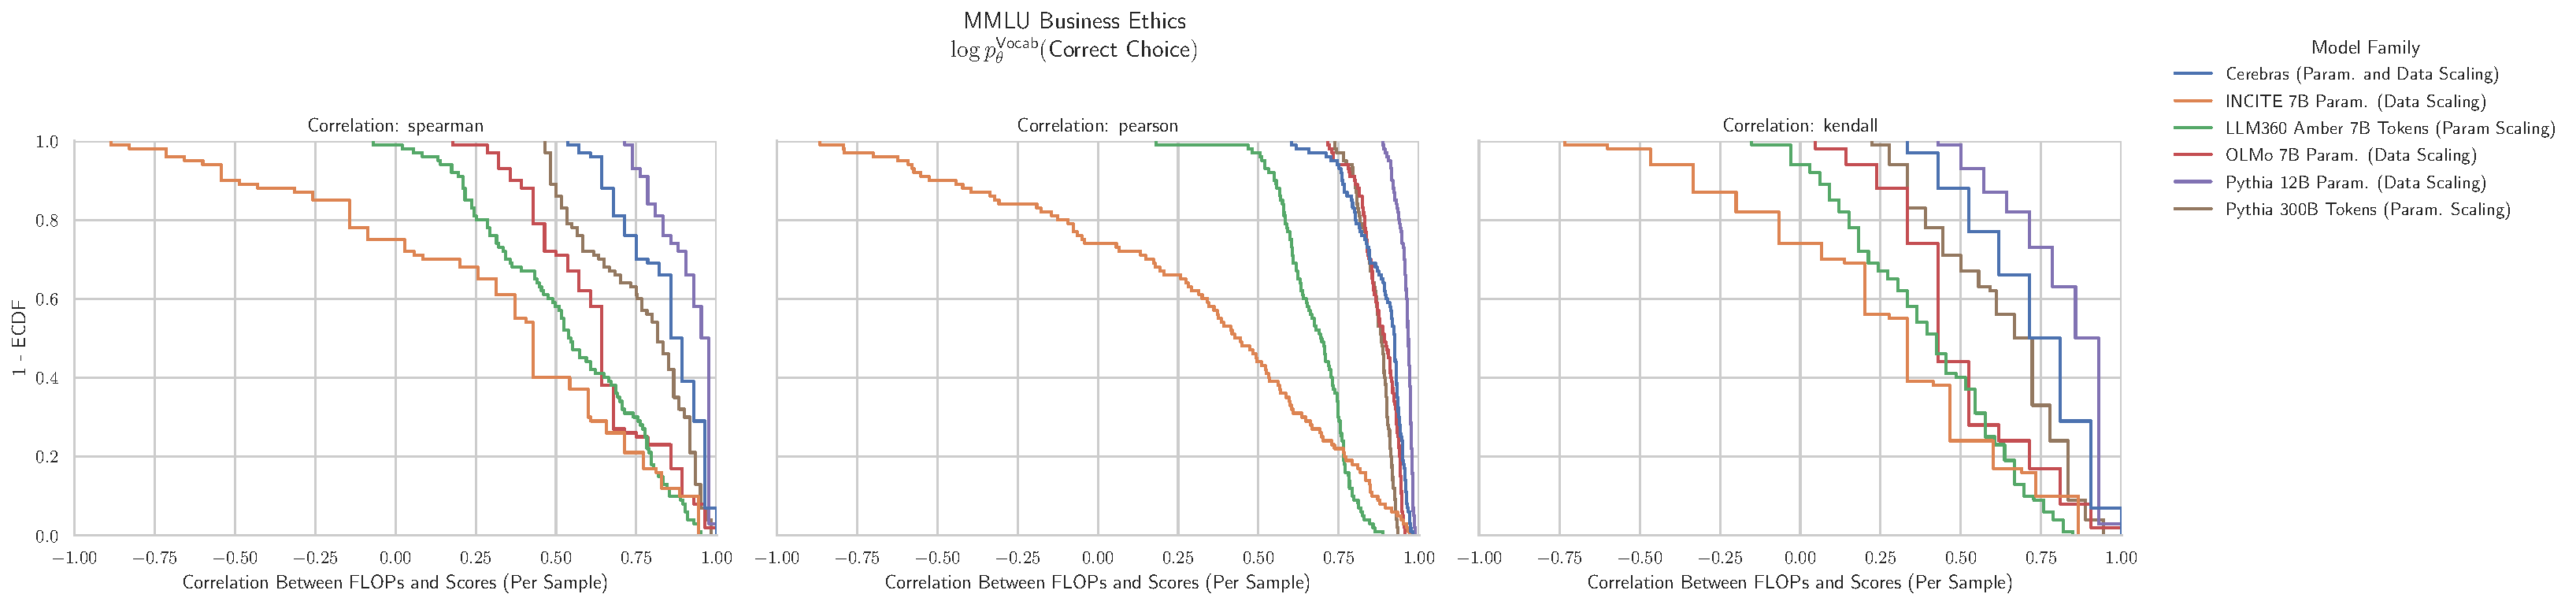
\includegraphics[width=\textwidth]{figures/correlations_between_scores_and_compute/correlation_distributions/mmlu_business_ethics/mmlu_business_ethics_log_likelihood_correct_ecdf_vs_correlation_score_by_modelfamily_split_correlation_metric.pdf}
    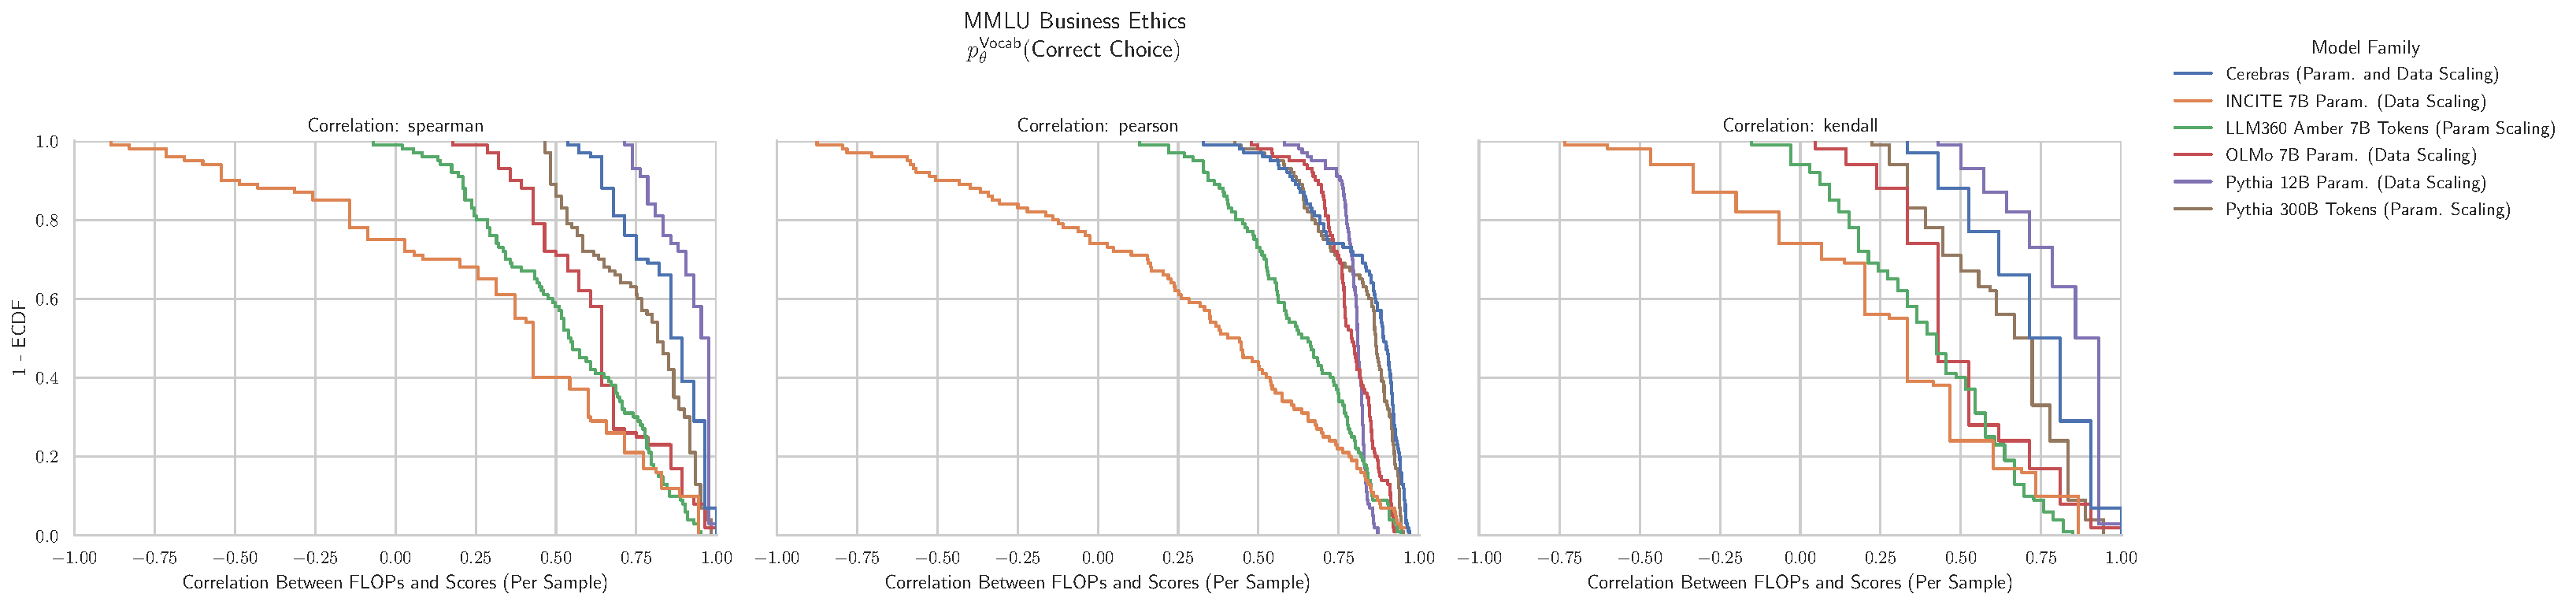
\includegraphics[width=\textwidth]{figures/correlations_between_scores_and_compute/correlation_distributions/mmlu_business_ethics/mmlu_business_ethics_prob_correct_vocab_ecdf_vs_correlation_score_by_modelfamily_split_correlation_metric.pdf}
    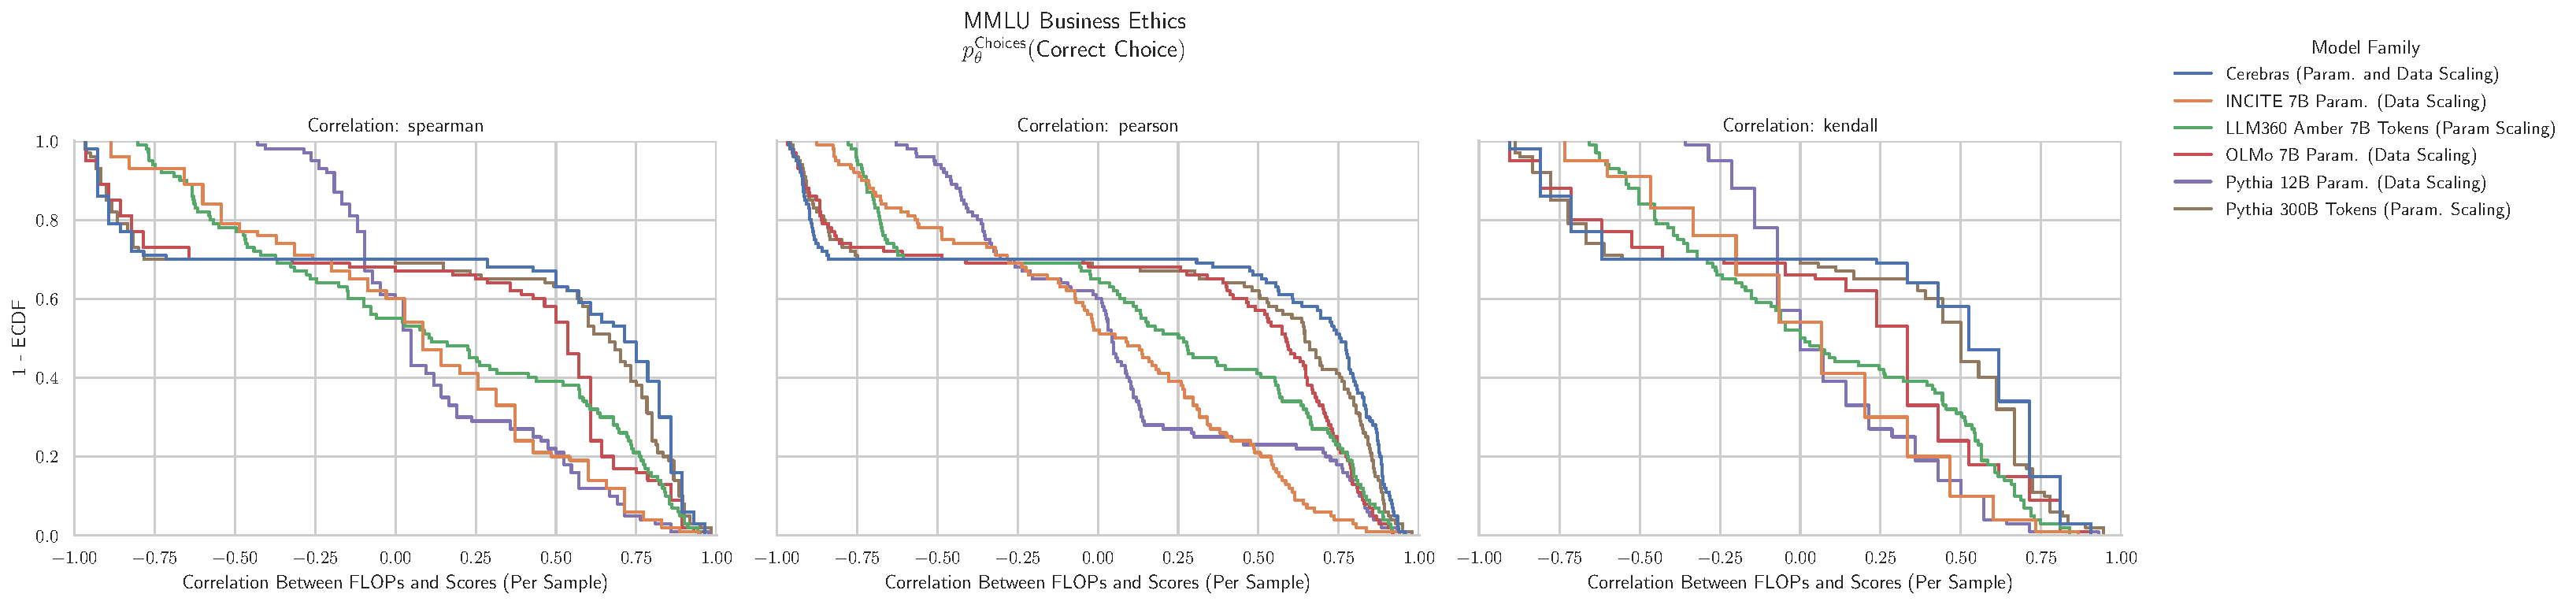
\includegraphics[width=\textwidth]{figures/correlations_between_scores_and_compute/correlation_distributions/mmlu_business_ethics/mmlu_business_ethics_prob_correct_choices_ecdf_vs_correlation_score_by_modelfamily_split_correlation_metric.pdf}
    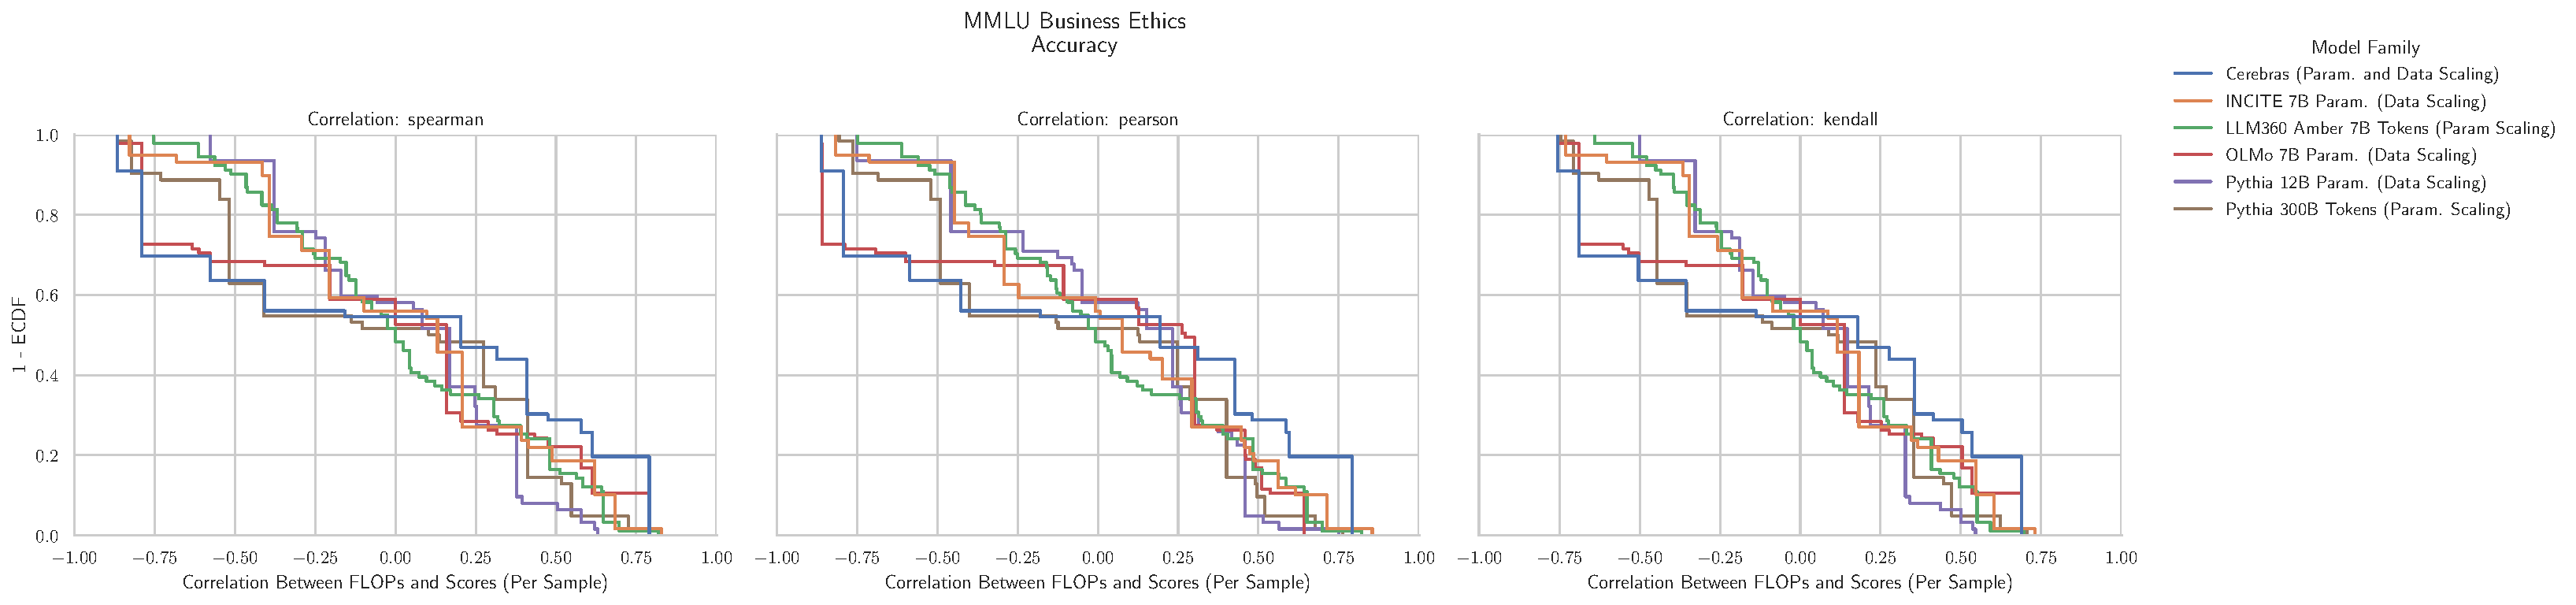
\includegraphics[width=\textwidth]{figures/correlations_between_scores_and_compute/correlation_distributions/mmlu_business_ethics/mmlu_business_ethics_acc_ecdf_vs_correlation_score_by_modelfamily_split_correlation_metric.pdf}
    \caption{\textbf{MMLU Business Ethics: Downstream performance is computed via a sequence of transformations that deteriorate correlations between scores and pretraining compute.}}
    \label{app:fig:compute_score_distribution_mmlu_business_ethics}
\end{figure}


\clearpage
\subsection{NLP Benchmark: MMLU Clinical Knowledge \cite{hendrycks2020mmlu}}

\begin{figure}[h!]
    \centering
    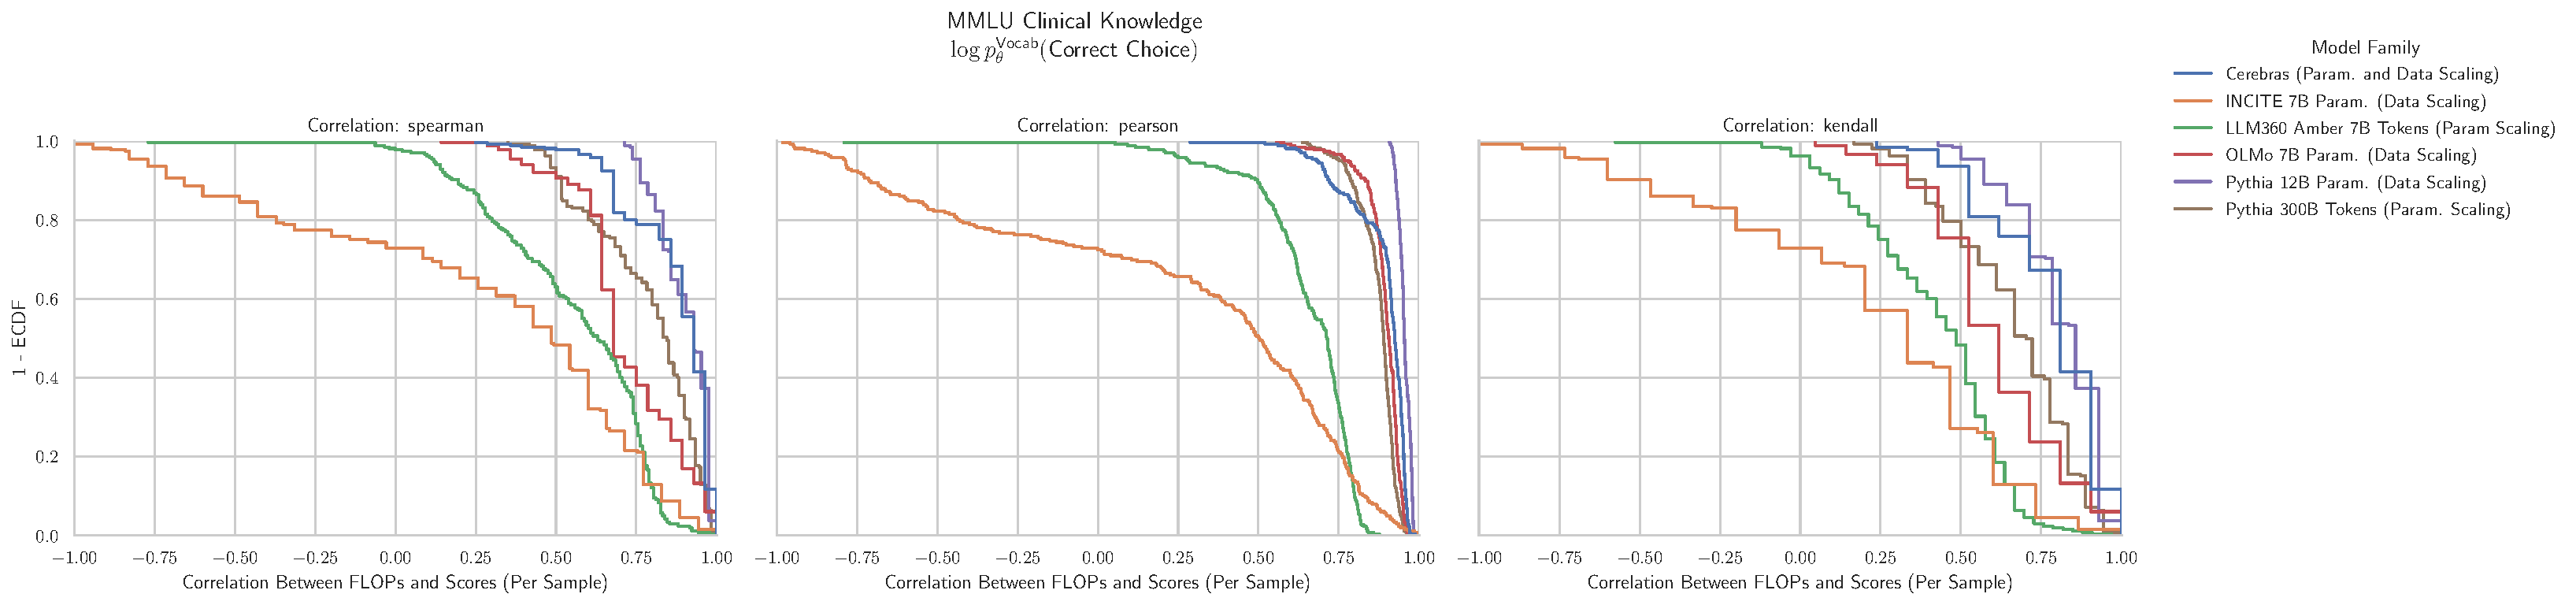
\includegraphics[width=\textwidth]{figures/correlations_between_scores_and_compute/correlation_distributions/mmlu_clinical_knowledge/mmlu_clinical_knowledge_log_likelihood_correct_ecdf_vs_correlation_score_by_modelfamily_split_correlation_metric.pdf}
    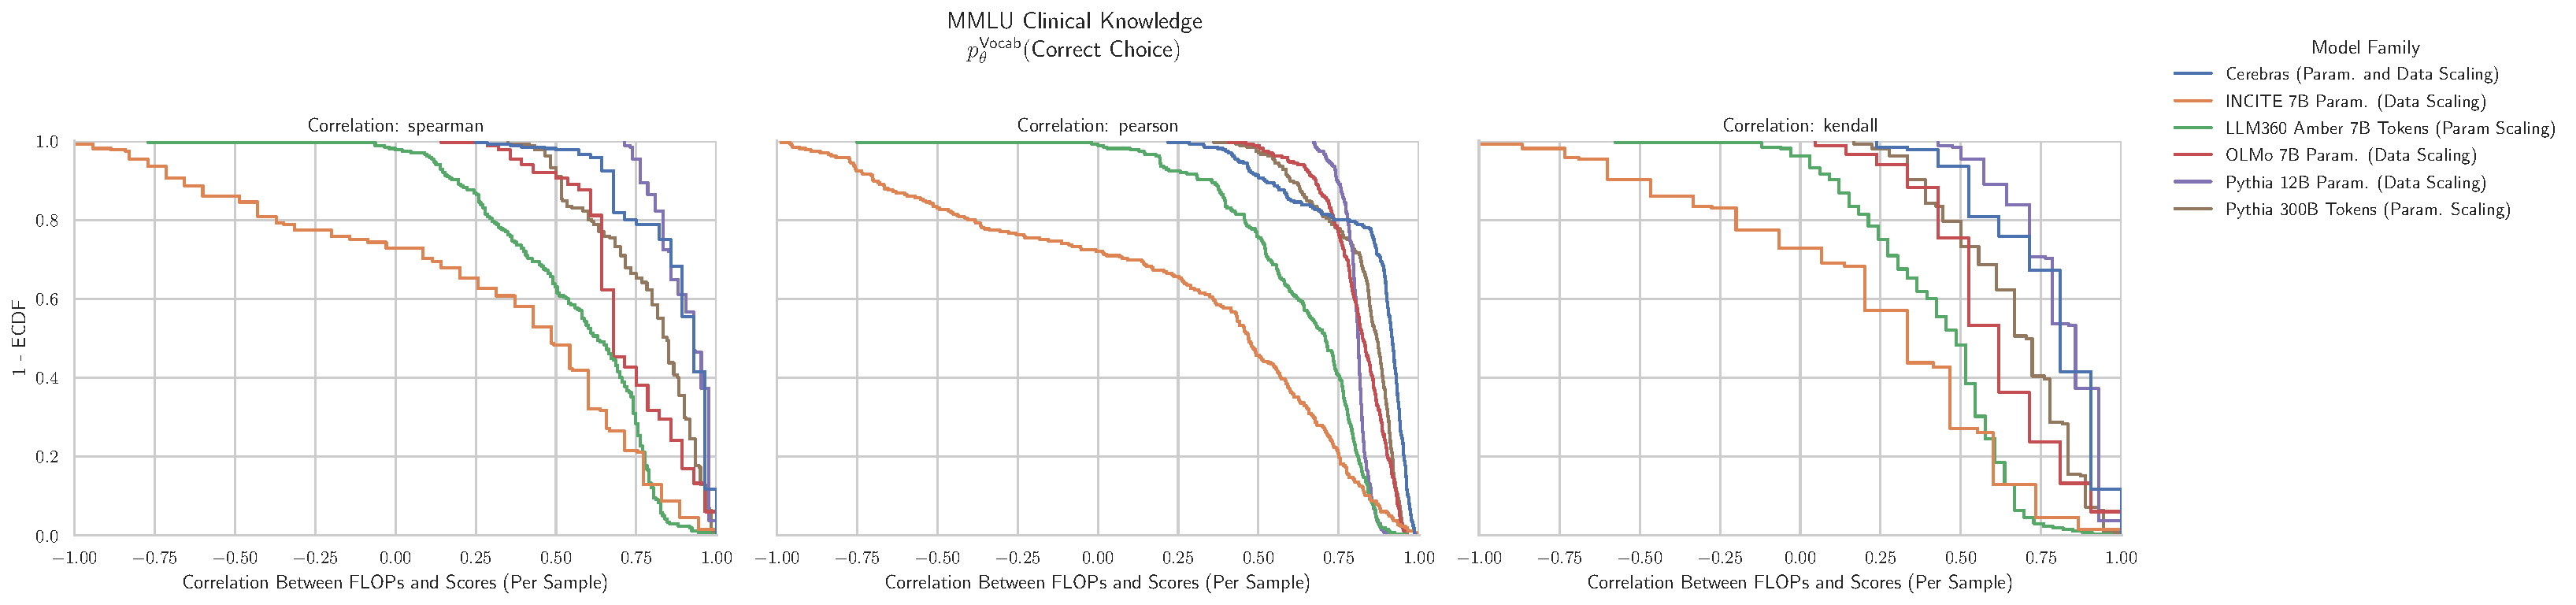
\includegraphics[width=\textwidth]{figures/correlations_between_scores_and_compute/correlation_distributions/mmlu_clinical_knowledge/mmlu_clinical_knowledge_prob_correct_vocab_ecdf_vs_correlation_score_by_modelfamily_split_correlation_metric.pdf}
    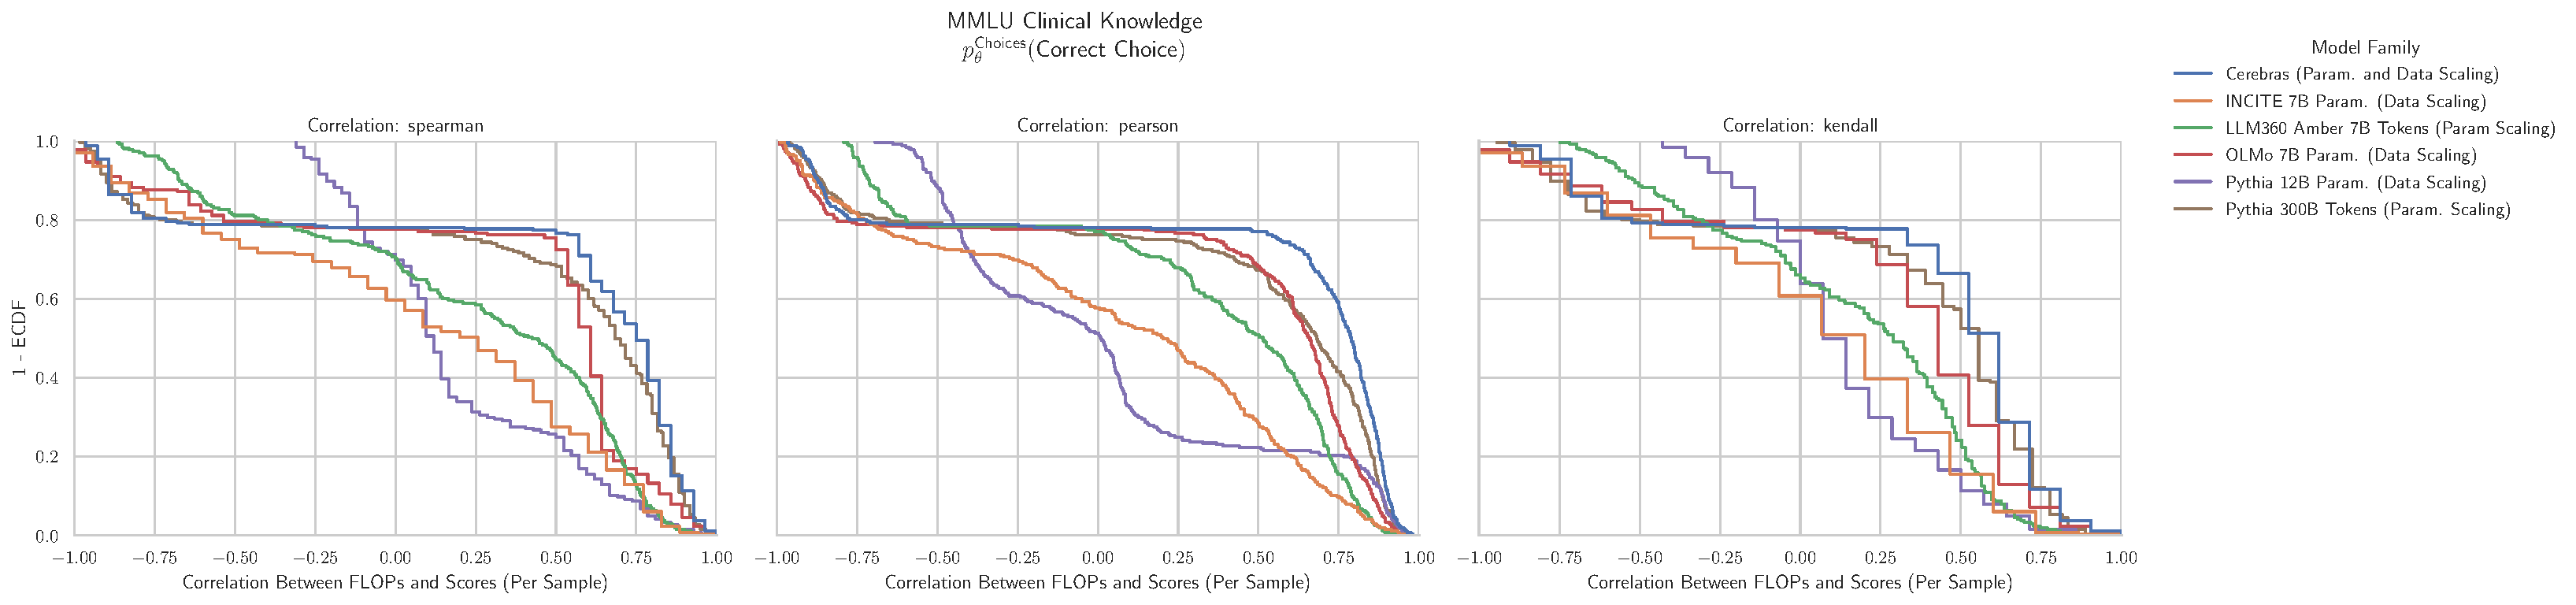
\includegraphics[width=\textwidth]{figures/correlations_between_scores_and_compute/correlation_distributions/mmlu_clinical_knowledge/mmlu_clinical_knowledge_prob_correct_choices_ecdf_vs_correlation_score_by_modelfamily_split_correlation_metric.pdf}
    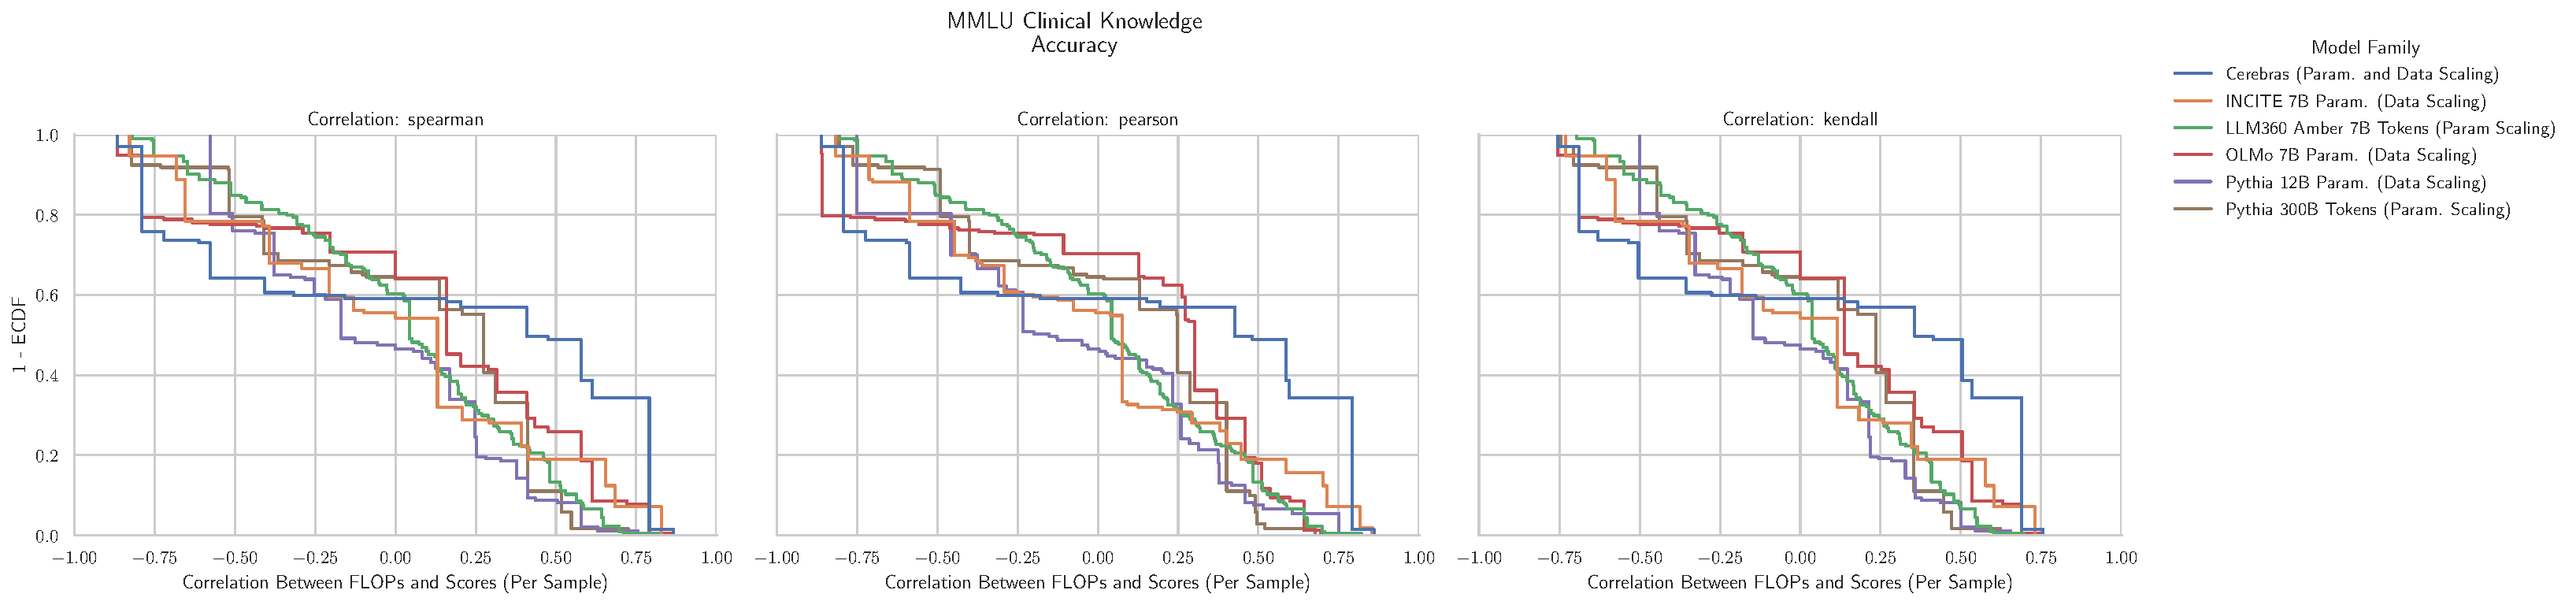
\includegraphics[width=\textwidth]{figures/correlations_between_scores_and_compute/correlation_distributions/mmlu_clinical_knowledge/mmlu_clinical_knowledge_acc_ecdf_vs_correlation_score_by_modelfamily_split_correlation_metric.pdf}
    \caption{\textbf{MMLU Clinical Knowledge: Downstream performance is computed via a sequence of transformations that deteriorate correlations between scores and pretraining compute.}}
    \label{app:fig:compute_score_distribution_mmlu_clinical_knowledge}
\end{figure}

\clearpage
\subsection{NLP Benchmark: MMLU College Biology \cite{hendrycks2020mmlu}}

\begin{figure}[h!]
    \centering
    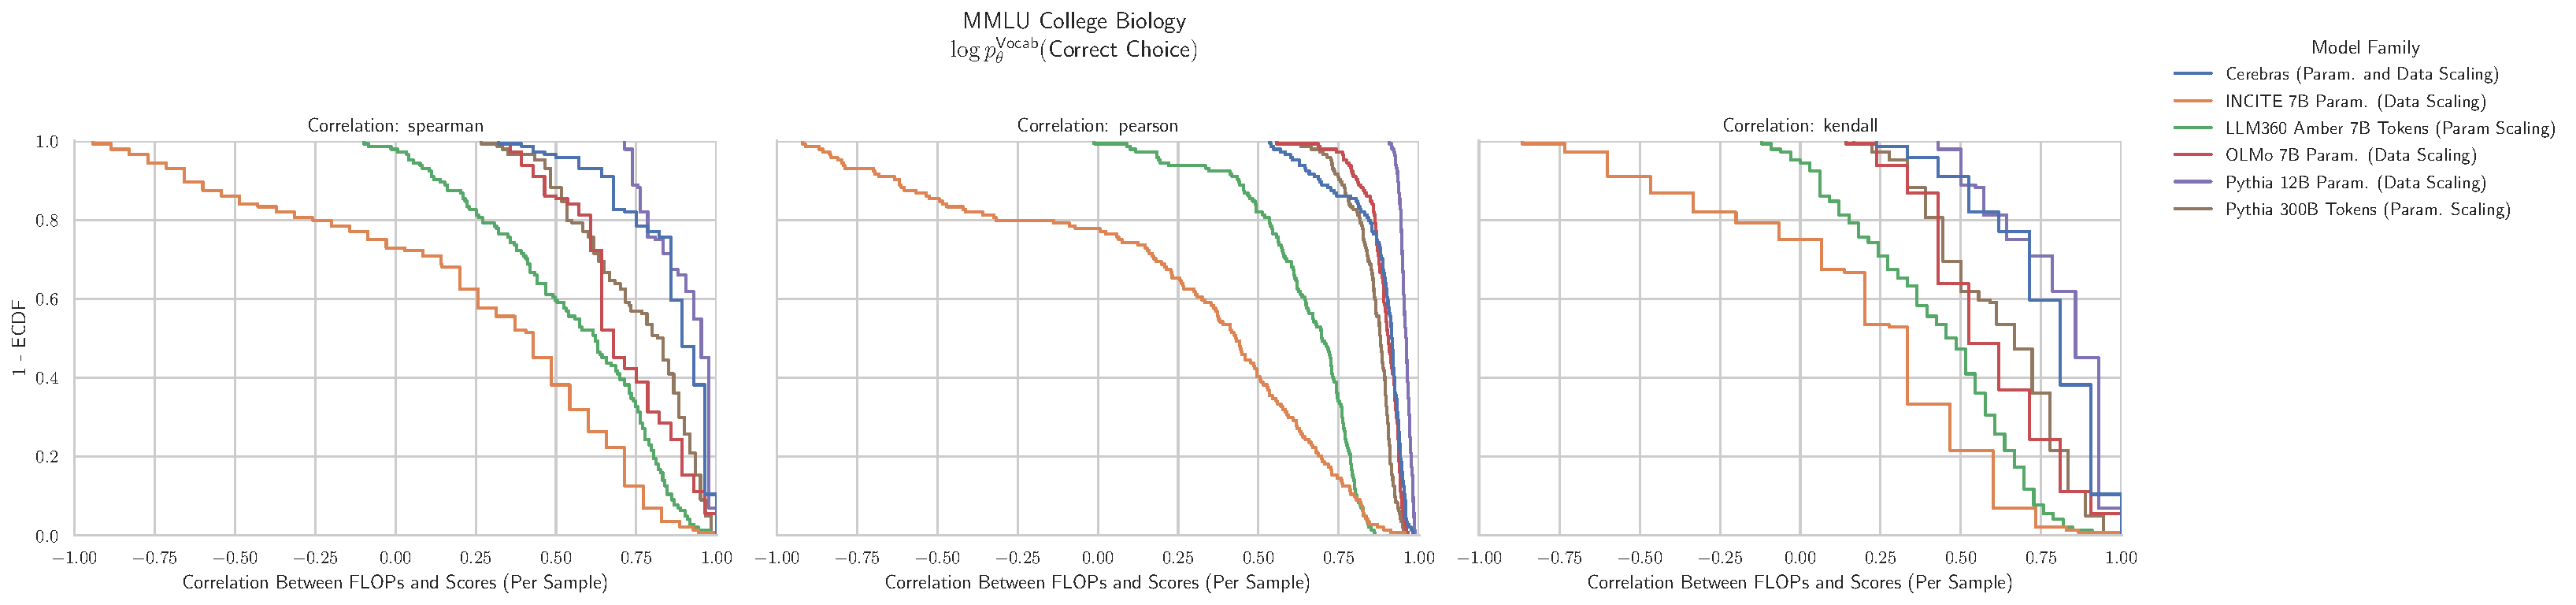
\includegraphics[width=\textwidth]{figures/correlations_between_scores_and_compute/correlation_distributions/mmlu_college_biology/mmlu_college_biology_log_likelihood_correct_ecdf_vs_correlation_score_by_modelfamily_split_correlation_metric.pdf}
    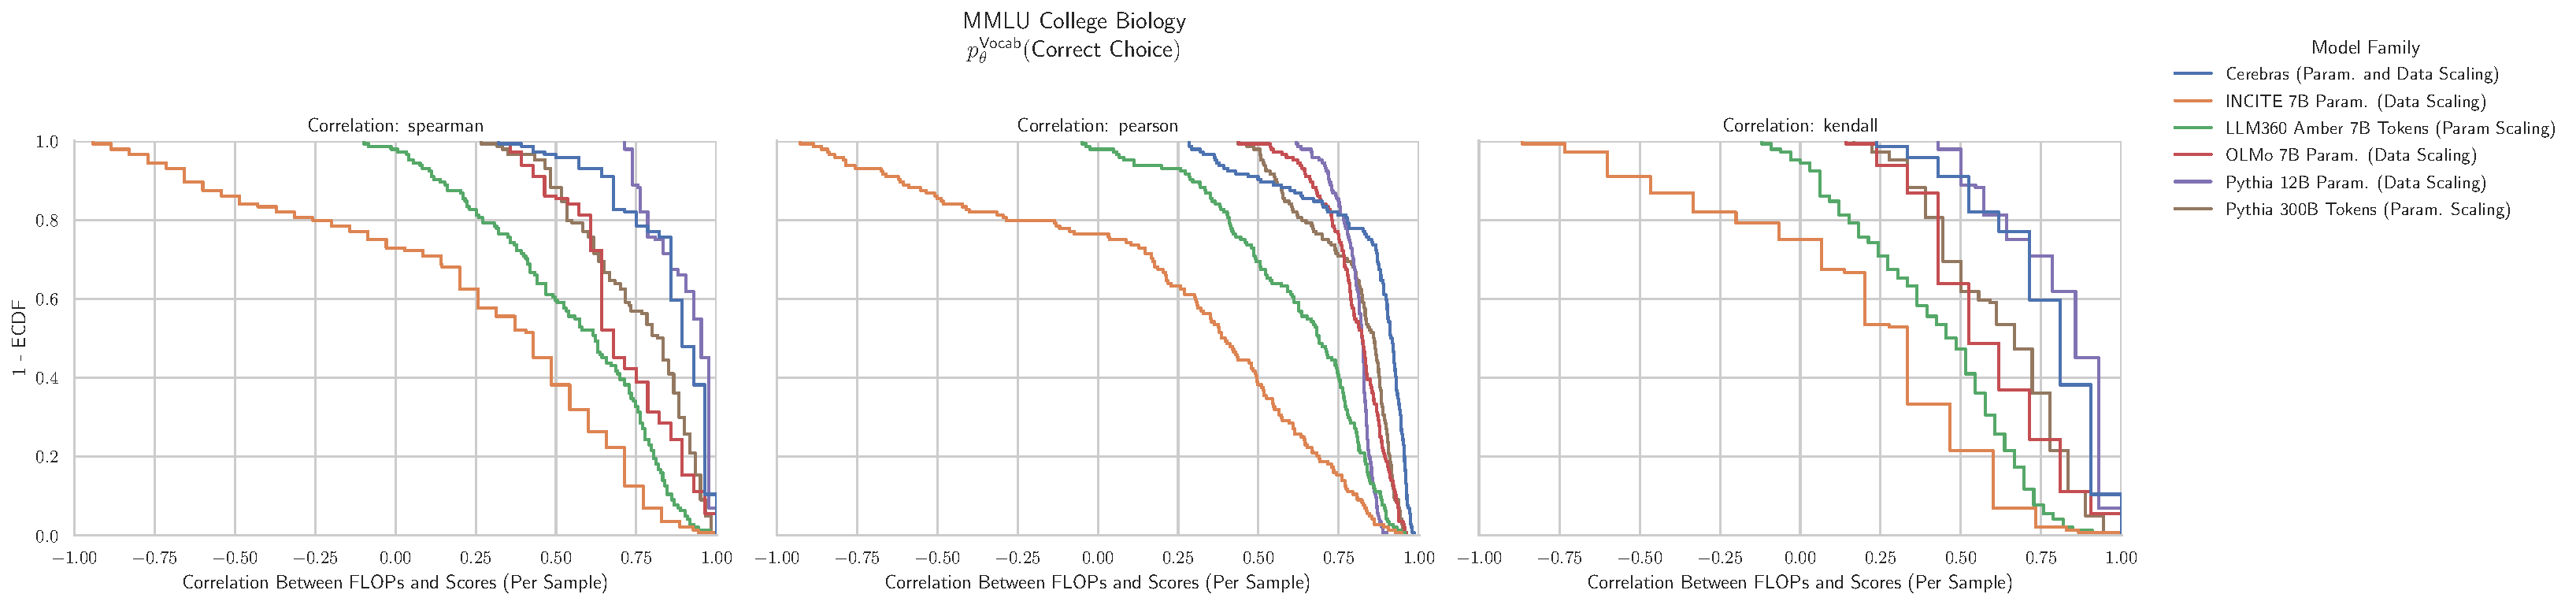
\includegraphics[width=\textwidth]{figures/correlations_between_scores_and_compute/correlation_distributions/mmlu_college_biology/mmlu_college_biology_prob_correct_vocab_ecdf_vs_correlation_score_by_modelfamily_split_correlation_metric.pdf}
    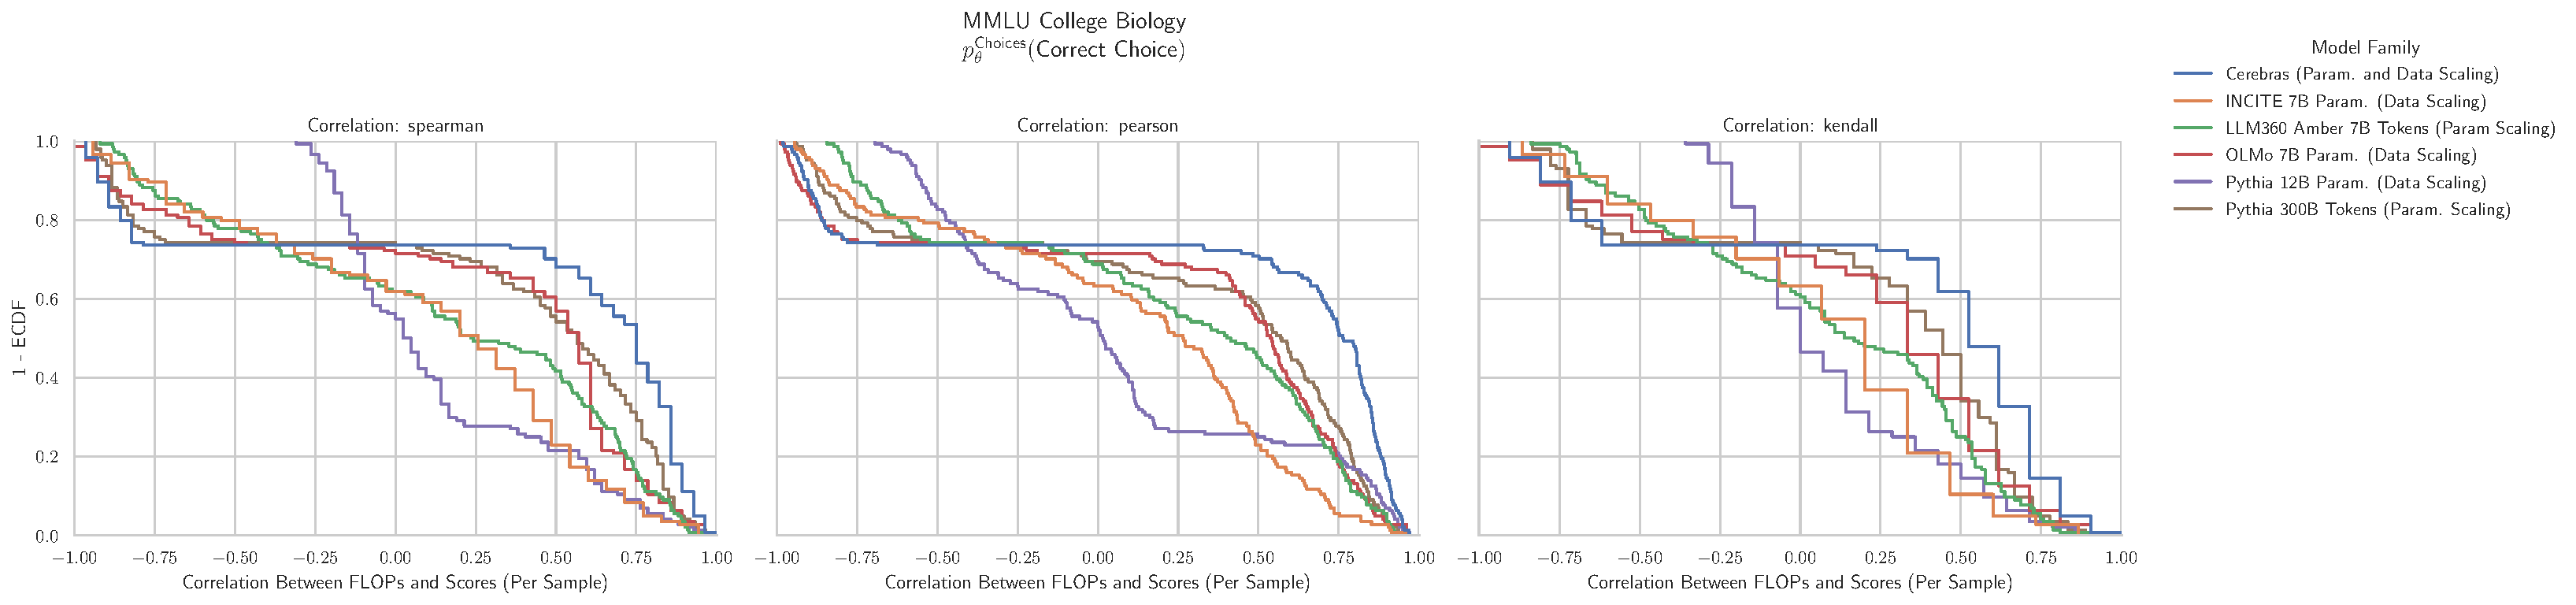
\includegraphics[width=\textwidth]{figures/correlations_between_scores_and_compute/correlation_distributions/mmlu_college_biology/mmlu_college_biology_prob_correct_choices_ecdf_vs_correlation_score_by_modelfamily_split_correlation_metric.pdf}
    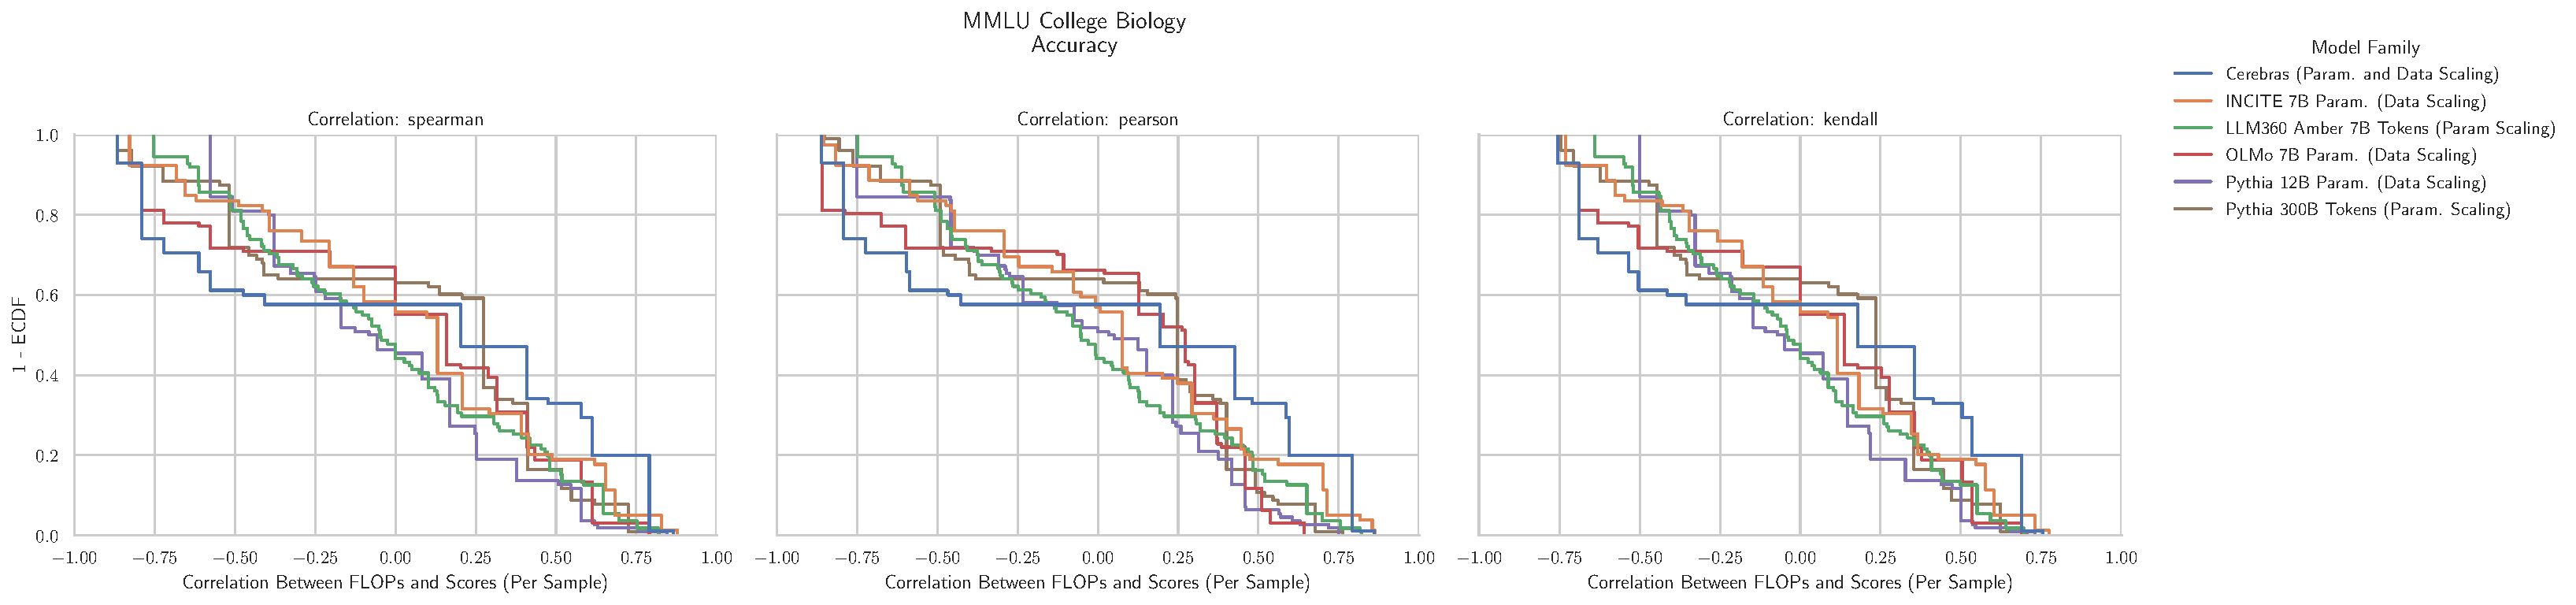
\includegraphics[width=\textwidth]{figures/correlations_between_scores_and_compute/correlation_distributions/mmlu_college_biology/mmlu_college_biology_acc_ecdf_vs_correlation_score_by_modelfamily_split_correlation_metric.pdf}
    \caption{\textbf{MMLU College Biology: Downstream performance is computed via a sequence of transformations that deteriorate correlations between scores and pretraining compute.}}
    \label{app:fig:compute_score_distribution_mmlu_college_biology}
\end{figure}

\clearpage
\subsection{NLP Benchmark: MMLU College Chemistry \cite{hendrycks2020mmlu}}

\begin{figure}[h!]
    \centering
    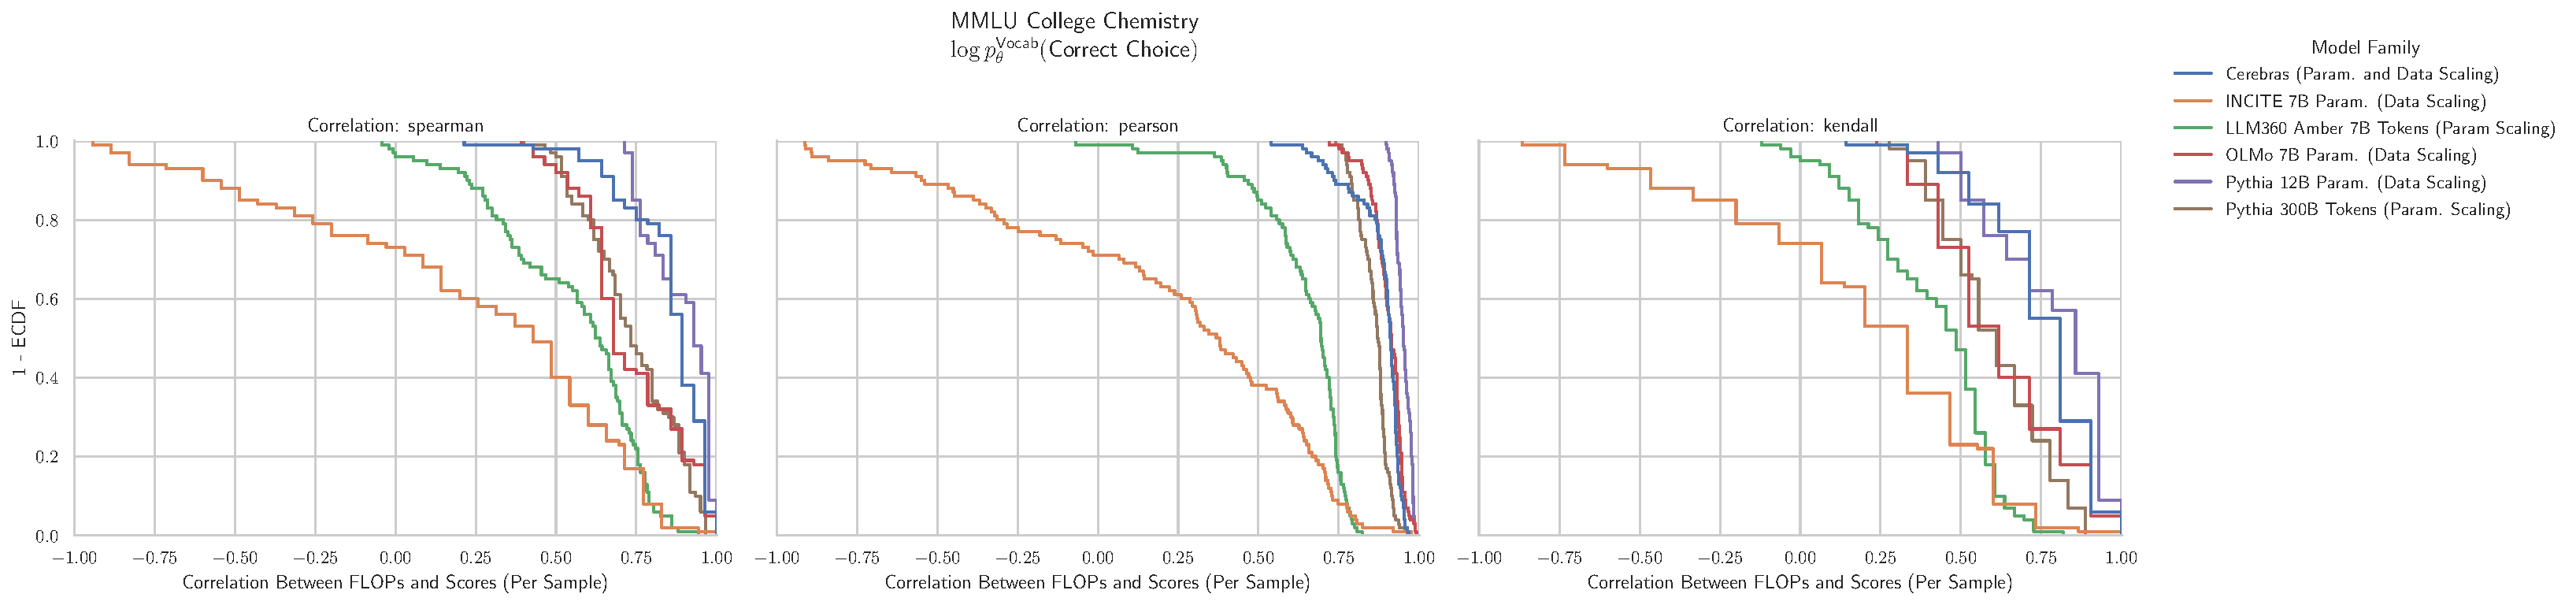
\includegraphics[width=\textwidth]{figures/correlations_between_scores_and_compute/correlation_distributions/mmlu_college_chemistry/mmlu_college_chemistry_log_likelihood_correct_ecdf_vs_correlation_score_by_modelfamily_split_correlation_metric.pdf}
    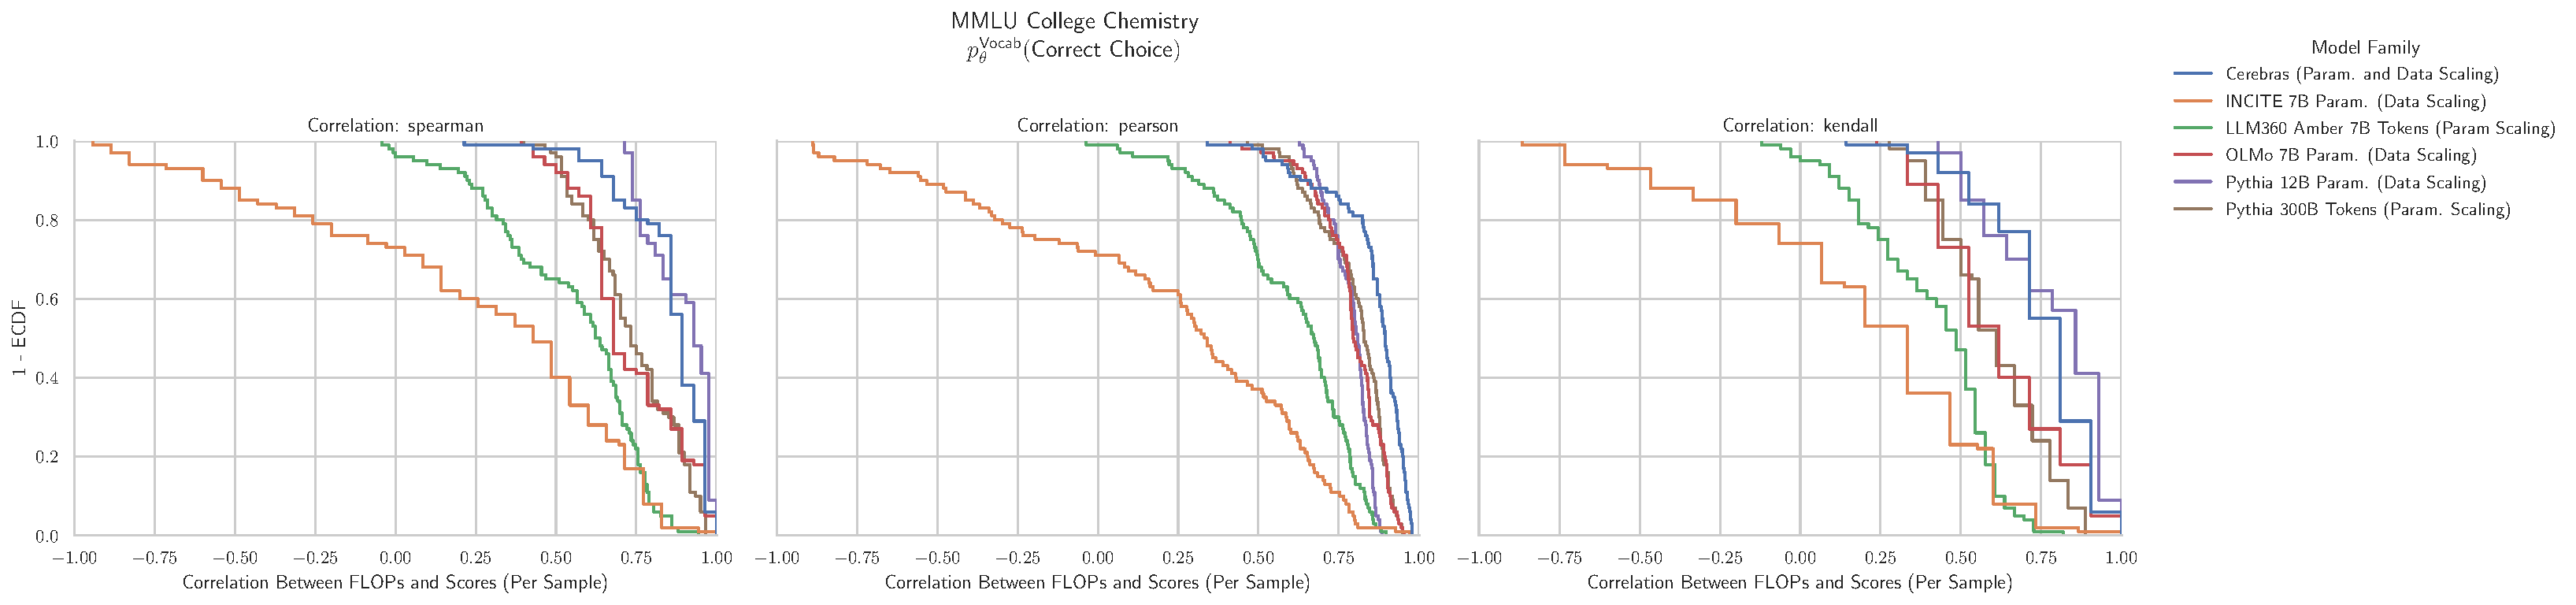
\includegraphics[width=\textwidth]{figures/correlations_between_scores_and_compute/correlation_distributions/mmlu_college_chemistry/mmlu_college_chemistry_prob_correct_vocab_ecdf_vs_correlation_score_by_modelfamily_split_correlation_metric.pdf}
    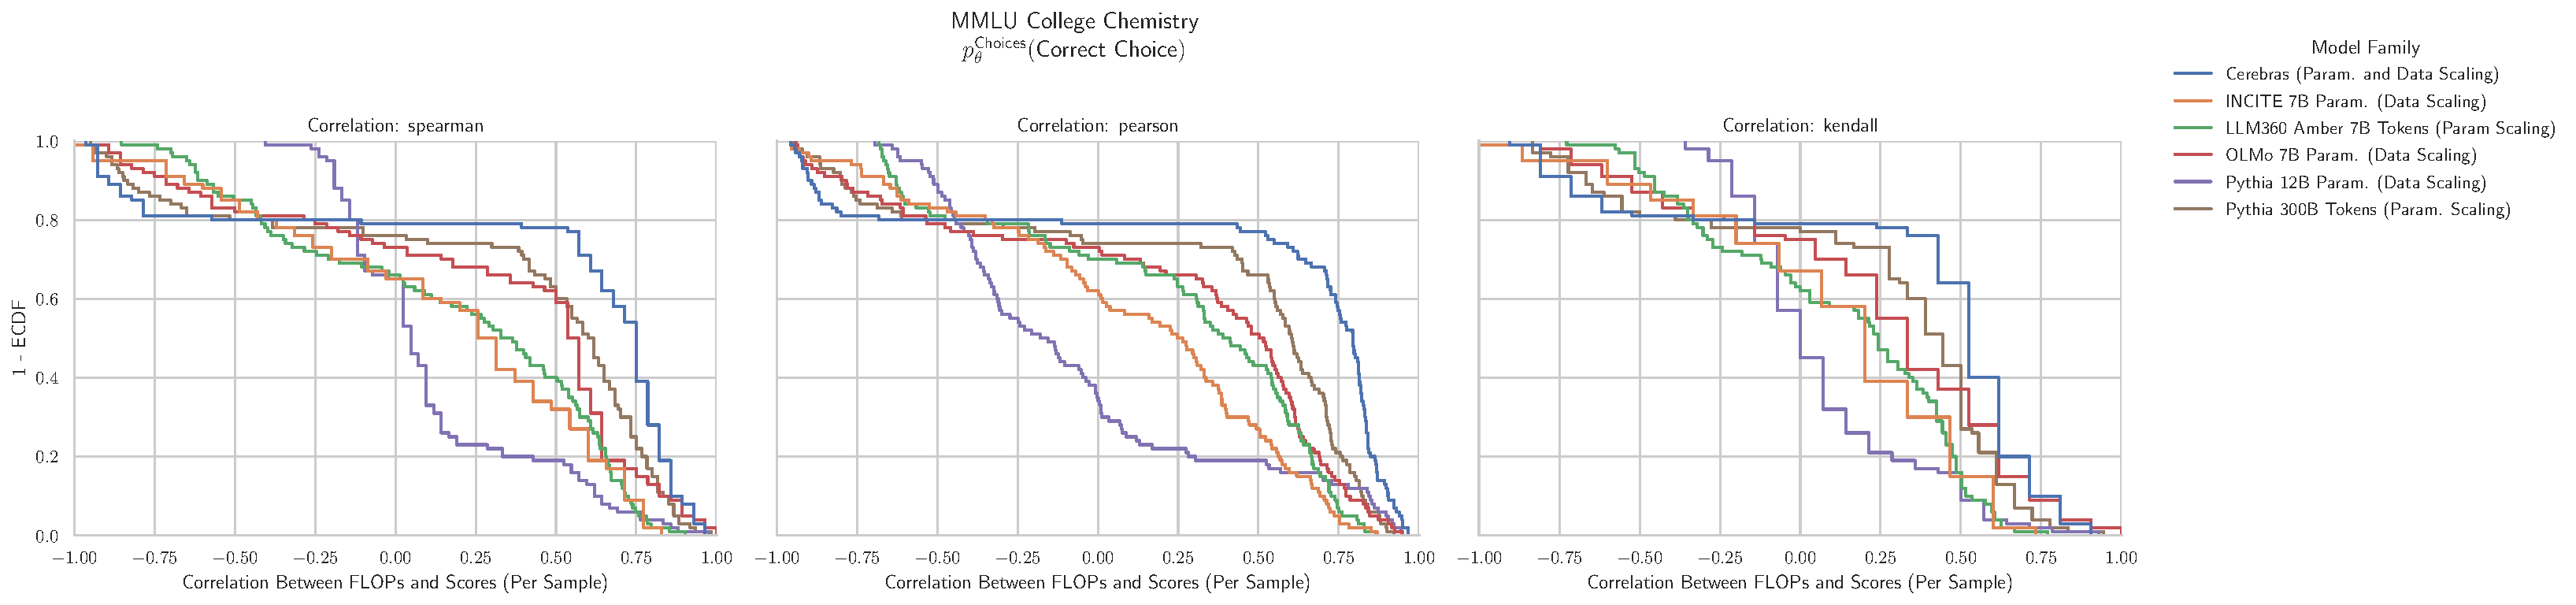
\includegraphics[width=\textwidth]{figures/correlations_between_scores_and_compute/correlation_distributions/mmlu_college_chemistry/mmlu_college_chemistry_prob_correct_choices_ecdf_vs_correlation_score_by_modelfamily_split_correlation_metric.pdf}
    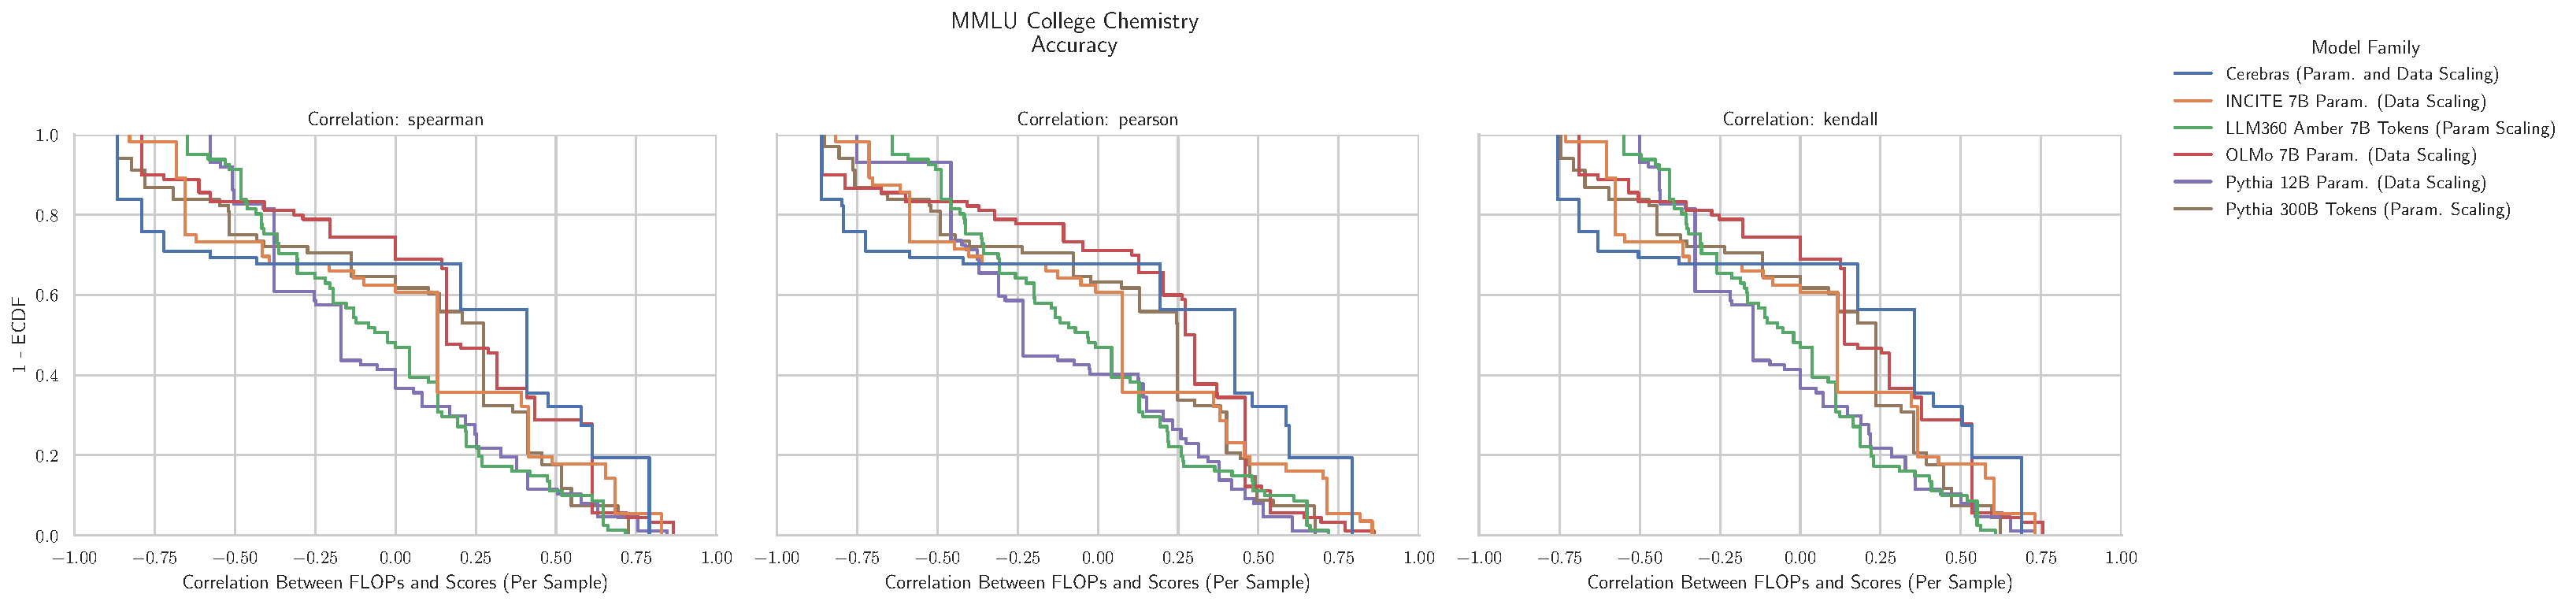
\includegraphics[width=\textwidth]{figures/correlations_between_scores_and_compute/correlation_distributions/mmlu_college_chemistry/mmlu_college_chemistry_acc_ecdf_vs_correlation_score_by_modelfamily_split_correlation_metric.pdf}
    \caption{\textbf{MMLU College Chemistry: Downstream performance is computed via a sequence of transformations that deteriorate correlations between scores and pretraining compute.}}
    \label{app:fig:compute_score_distribution_mmlu_college_chemistry}
\end{figure}

\clearpage
\subsection{NLP Benchmark: MMLU College Computer Science \cite{hendrycks2020mmlu}}

\begin{figure}[h!]
    \centering
    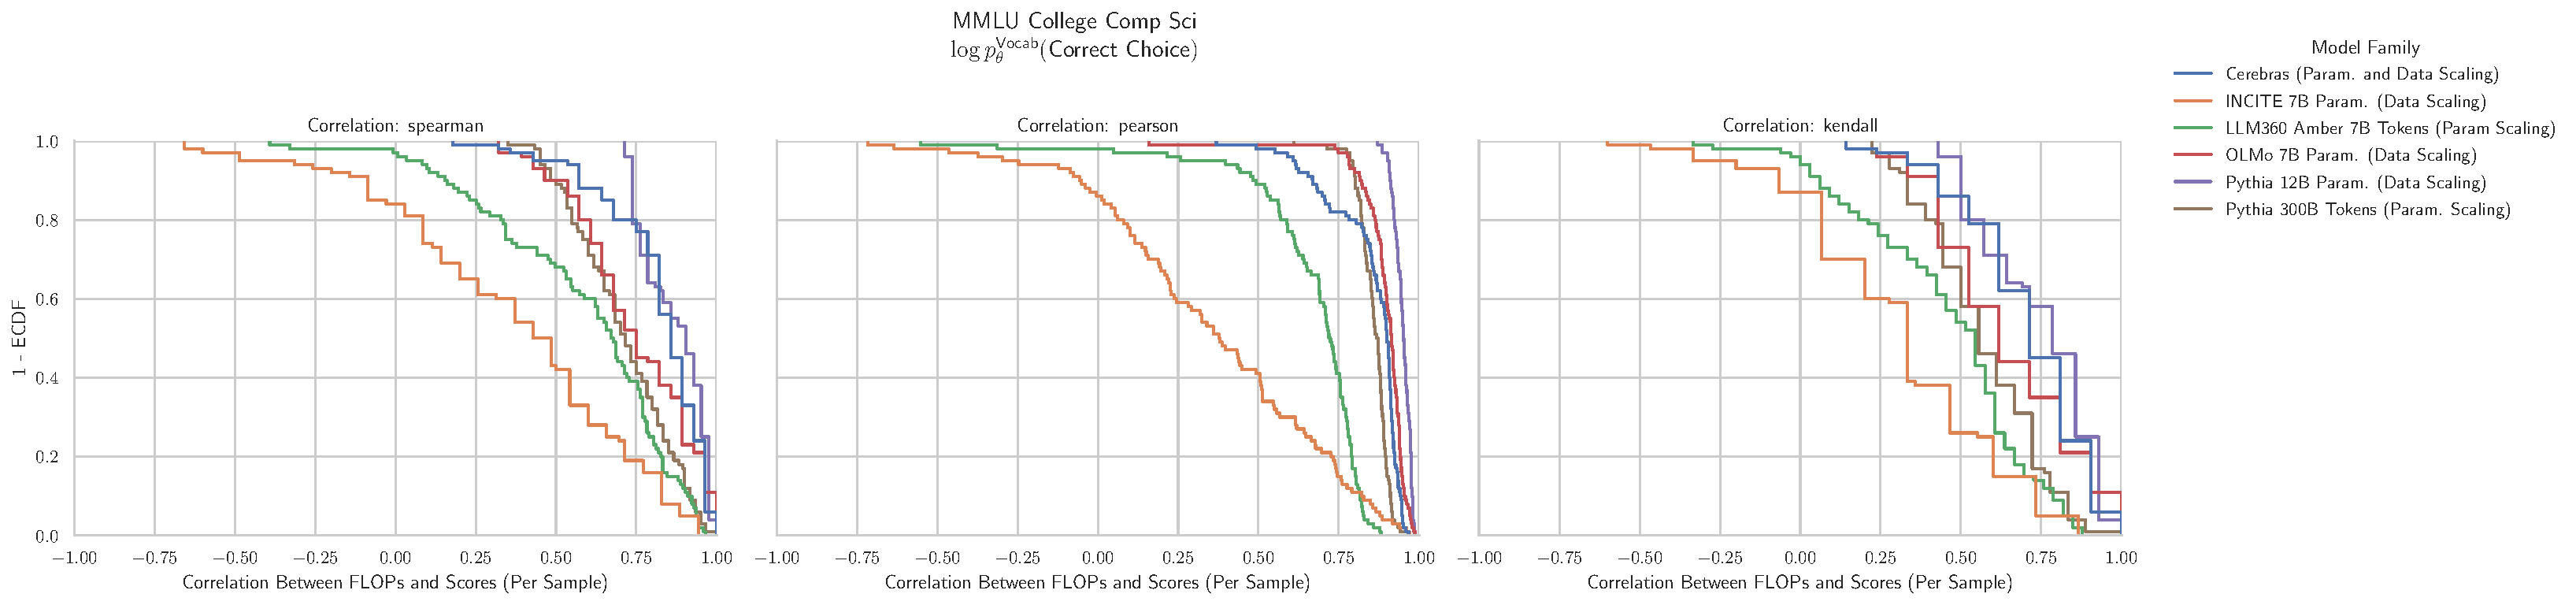
\includegraphics[width=\textwidth]{figures/correlations_between_scores_and_compute/correlation_distributions/mmlu_college_computer_science/mmlu_college_computer_science_log_likelihood_correct_ecdf_vs_correlation_score_by_modelfamily_split_correlation_metric.pdf}
    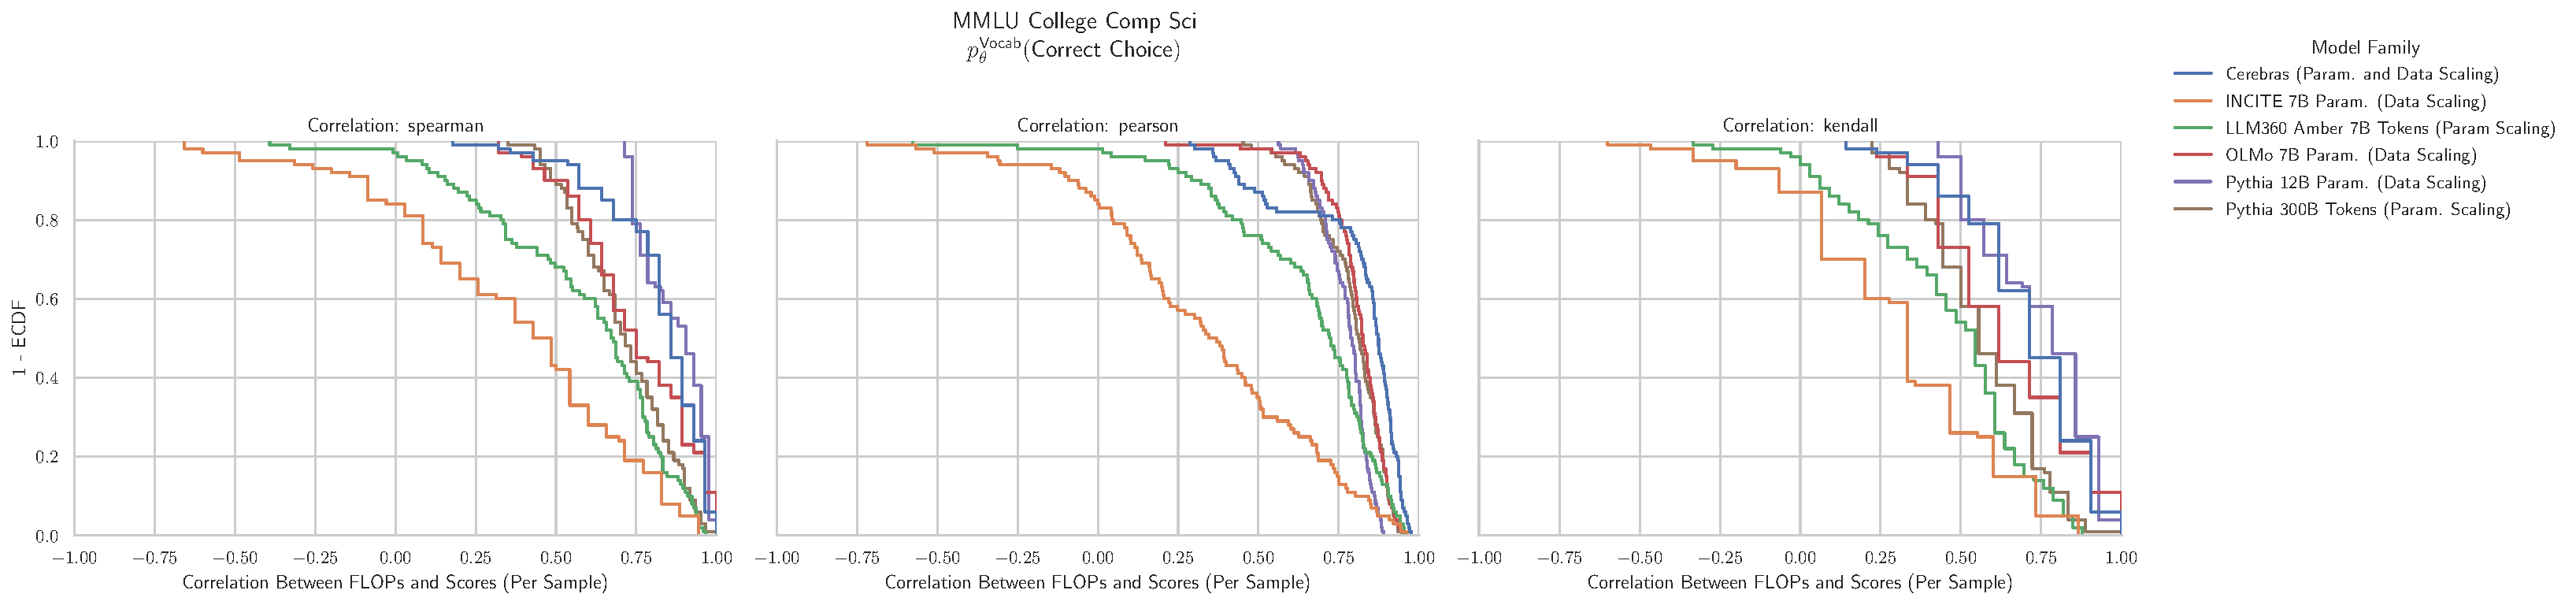
\includegraphics[width=\textwidth]{figures/correlations_between_scores_and_compute/correlation_distributions/mmlu_college_computer_science/mmlu_college_computer_science_prob_correct_vocab_ecdf_vs_correlation_score_by_modelfamily_split_correlation_metric.pdf}
    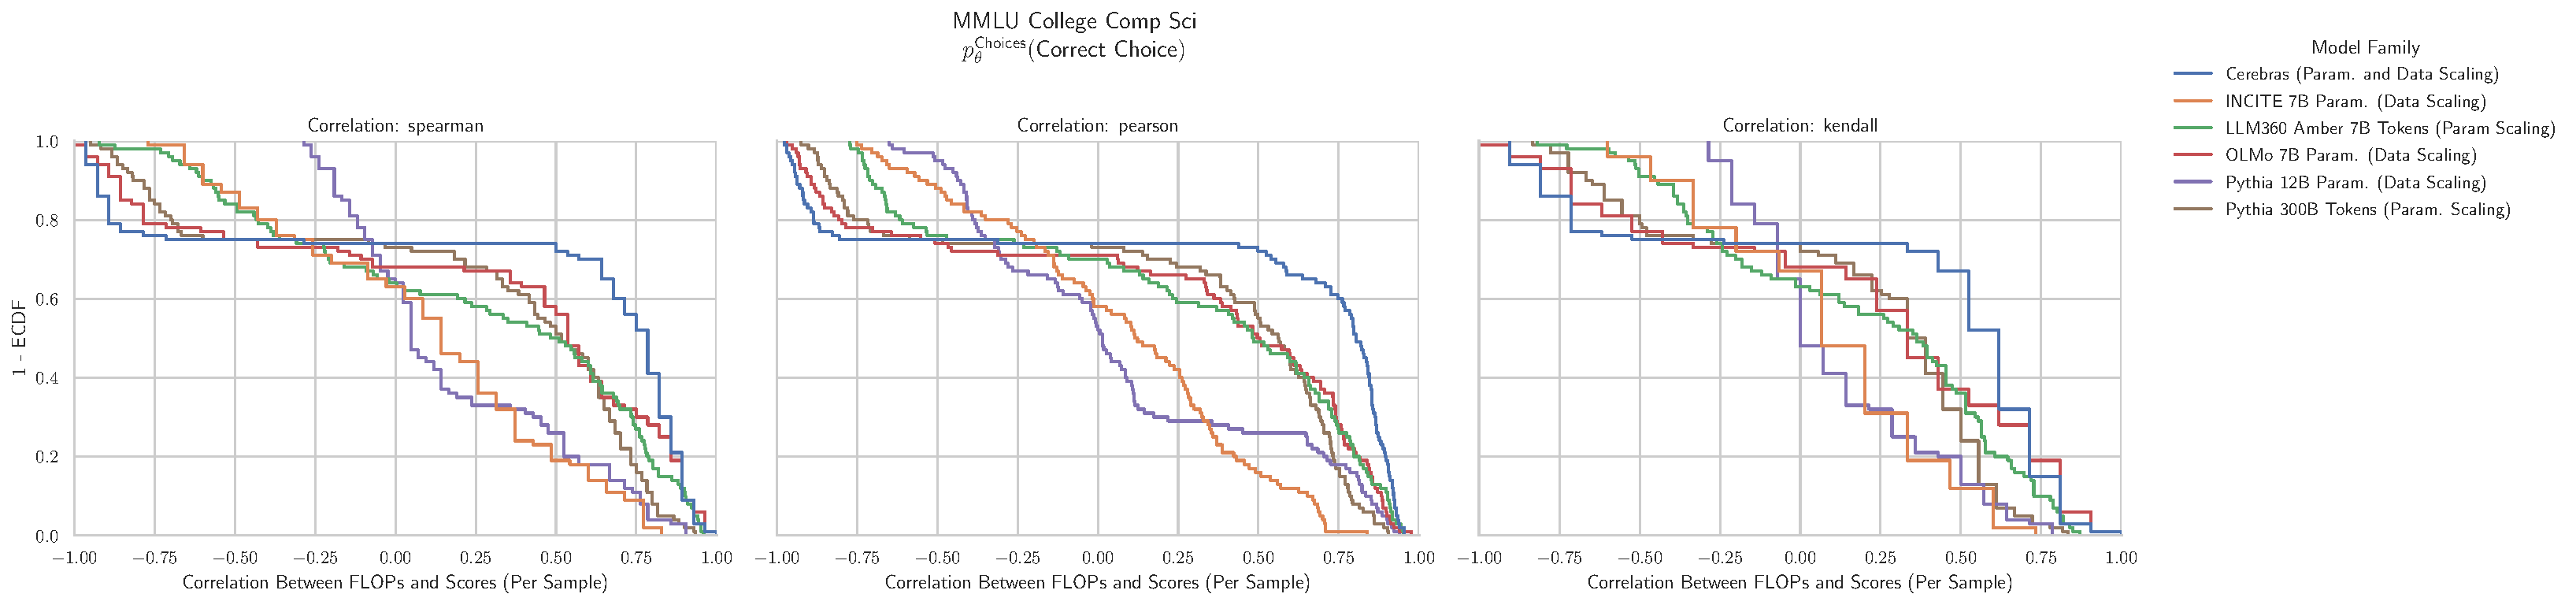
\includegraphics[width=\textwidth]{figures/correlations_between_scores_and_compute/correlation_distributions/mmlu_college_computer_science/mmlu_college_computer_science_prob_correct_choices_ecdf_vs_correlation_score_by_modelfamily_split_correlation_metric.pdf}
    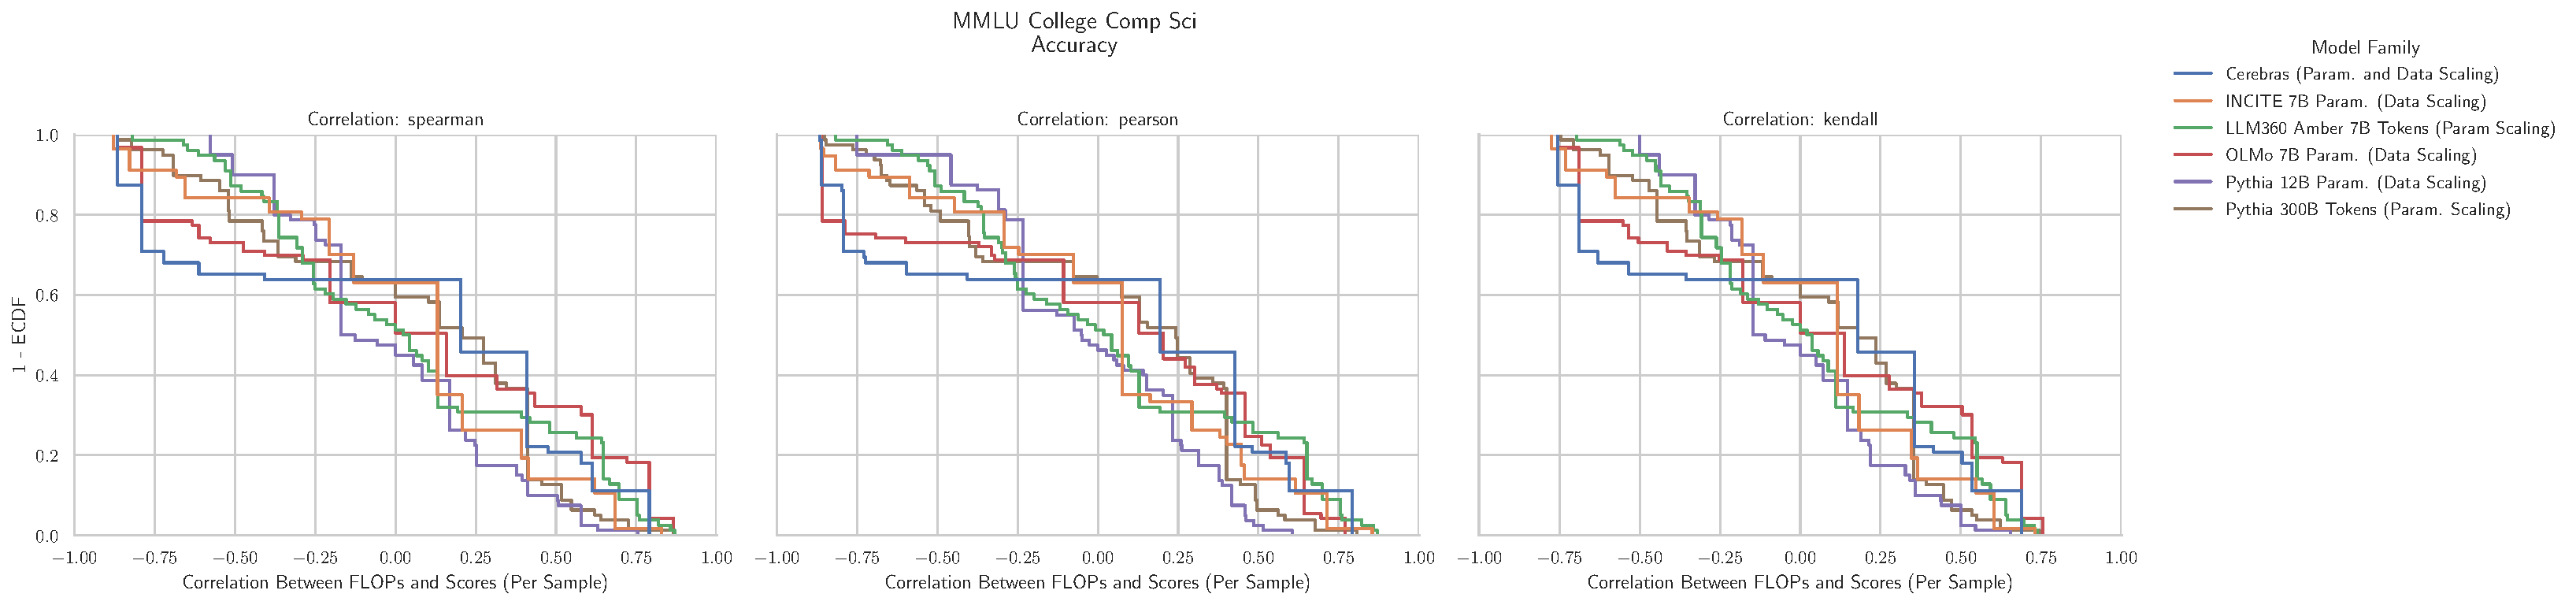
\includegraphics[width=\textwidth]{figures/correlations_between_scores_and_compute/correlation_distributions/mmlu_college_computer_science/mmlu_college_computer_science_acc_ecdf_vs_correlation_score_by_modelfamily_split_correlation_metric.pdf}
    \caption{\textbf{MMLU College Computer Science: Downstream performance is computed via a sequence of transformations that deteriorate correlations between scores and pretraining compute.}}
    \label{app:fig:compute_score_distribution_mmlu_college_computer_science}
\end{figure}


\clearpage
\subsection{NLP Benchmark: MMLU College Mathematics \cite{hendrycks2020mmlu}}

\begin{figure}[h!]
    \centering
    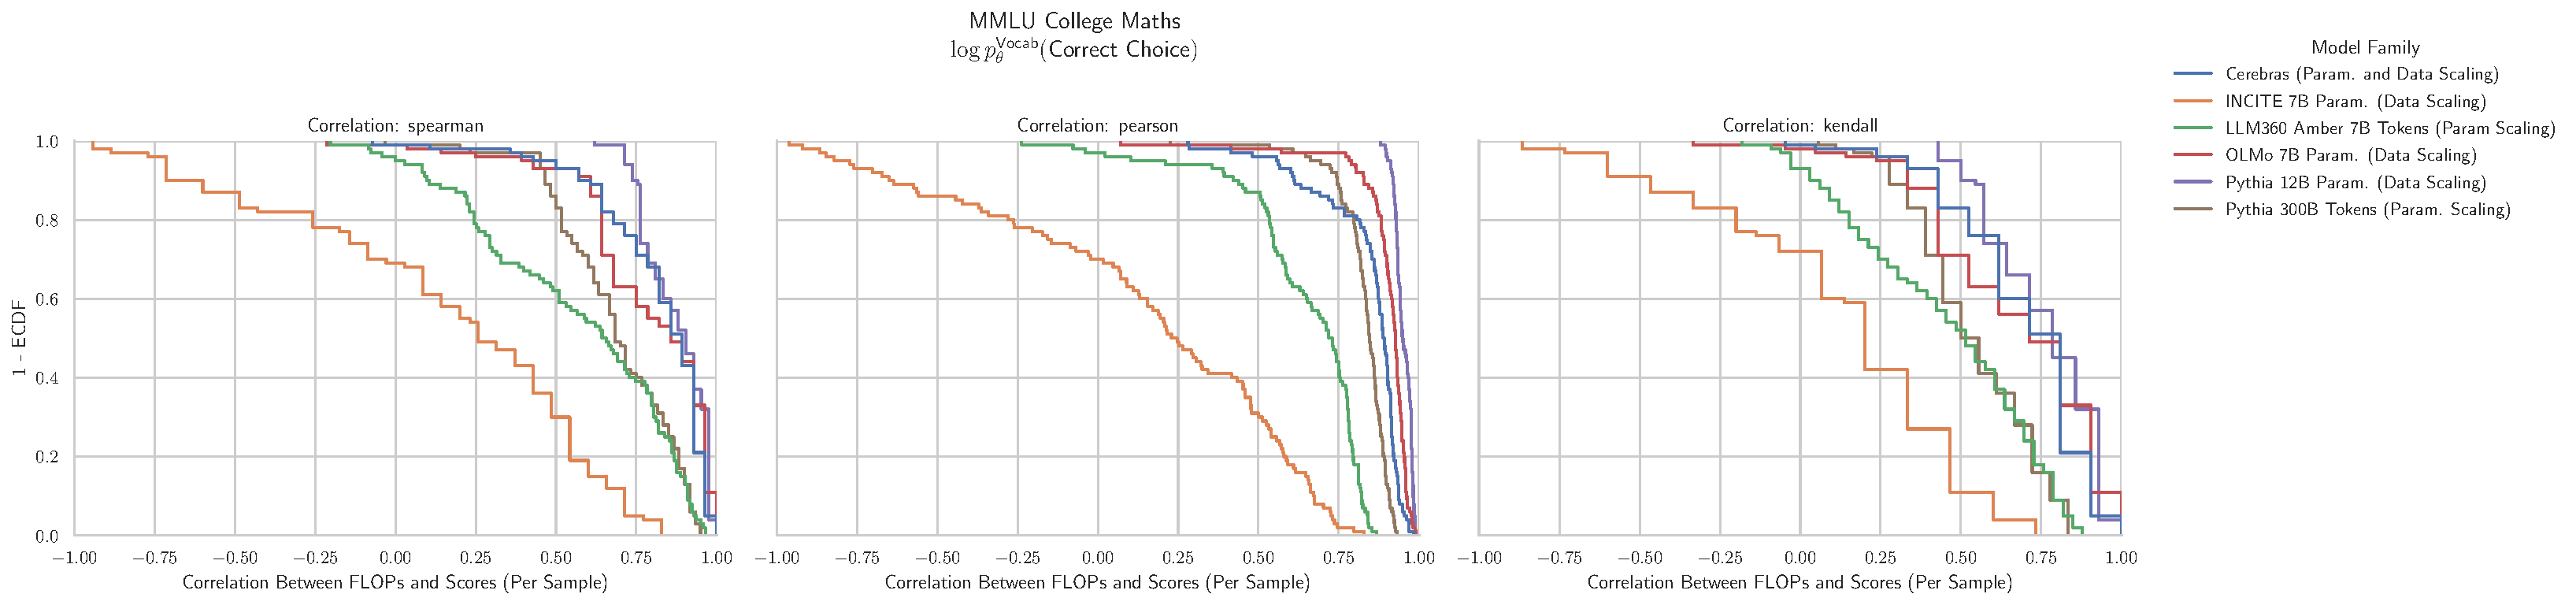
\includegraphics[width=\textwidth]{figures/correlations_between_scores_and_compute/correlation_distributions/mmlu_college_mathematics/mmlu_college_mathematics_log_likelihood_correct_ecdf_vs_correlation_score_by_modelfamily_split_correlation_metric.pdf}
    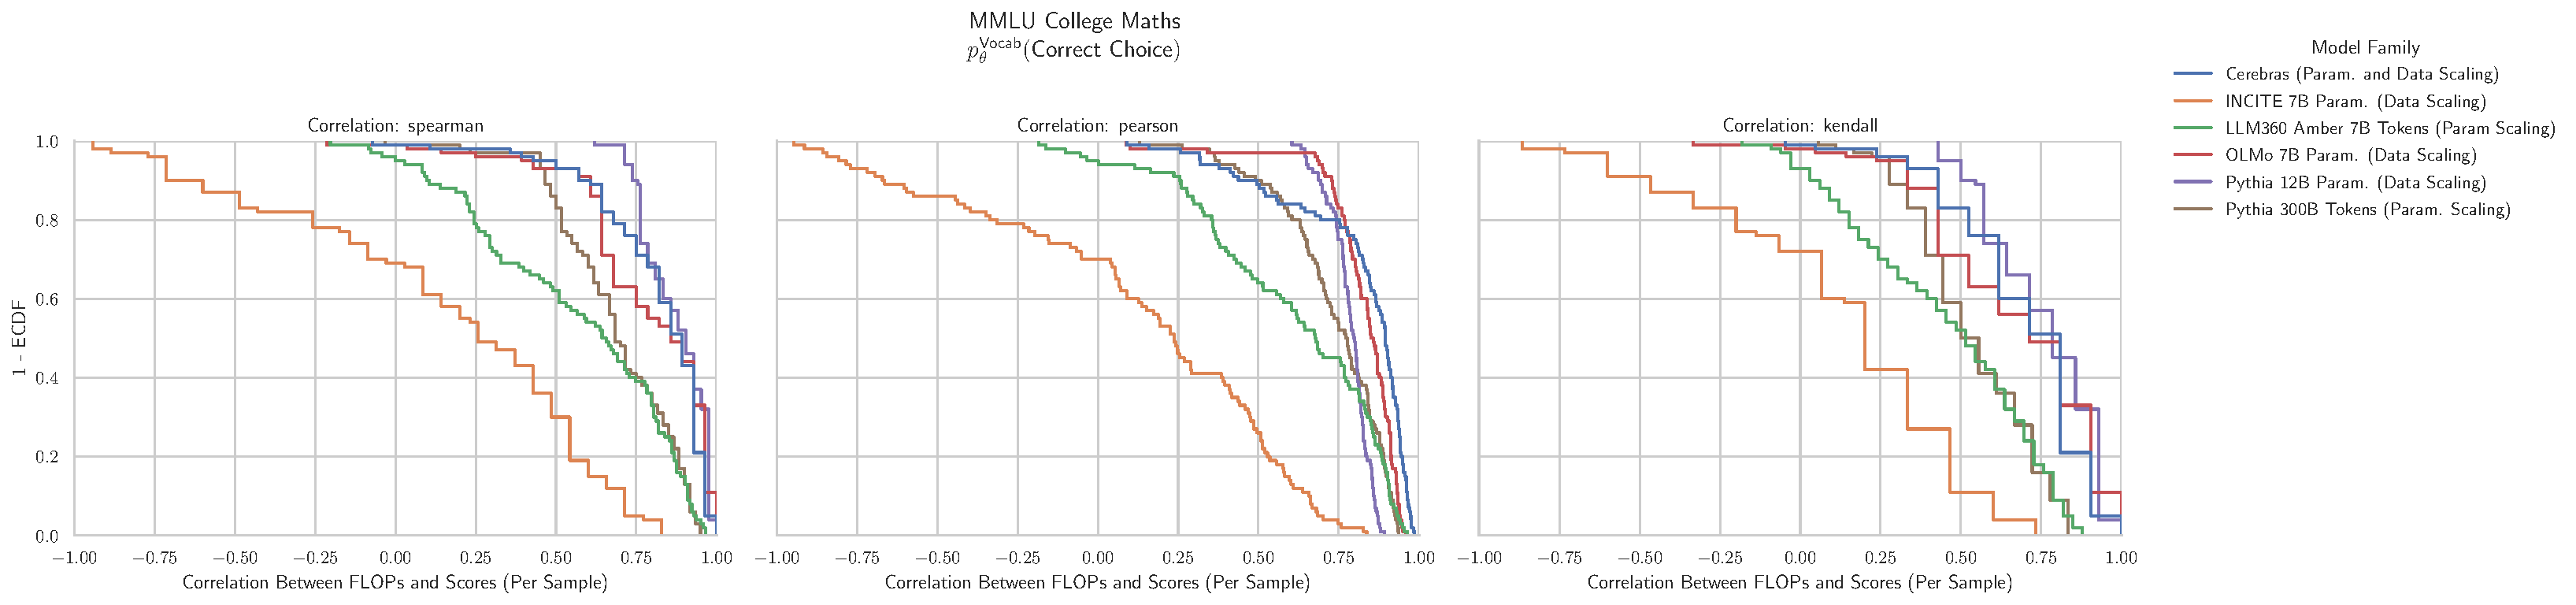
\includegraphics[width=\textwidth]{figures/correlations_between_scores_and_compute/correlation_distributions/mmlu_college_mathematics/mmlu_college_mathematics_prob_correct_vocab_ecdf_vs_correlation_score_by_modelfamily_split_correlation_metric.pdf}
    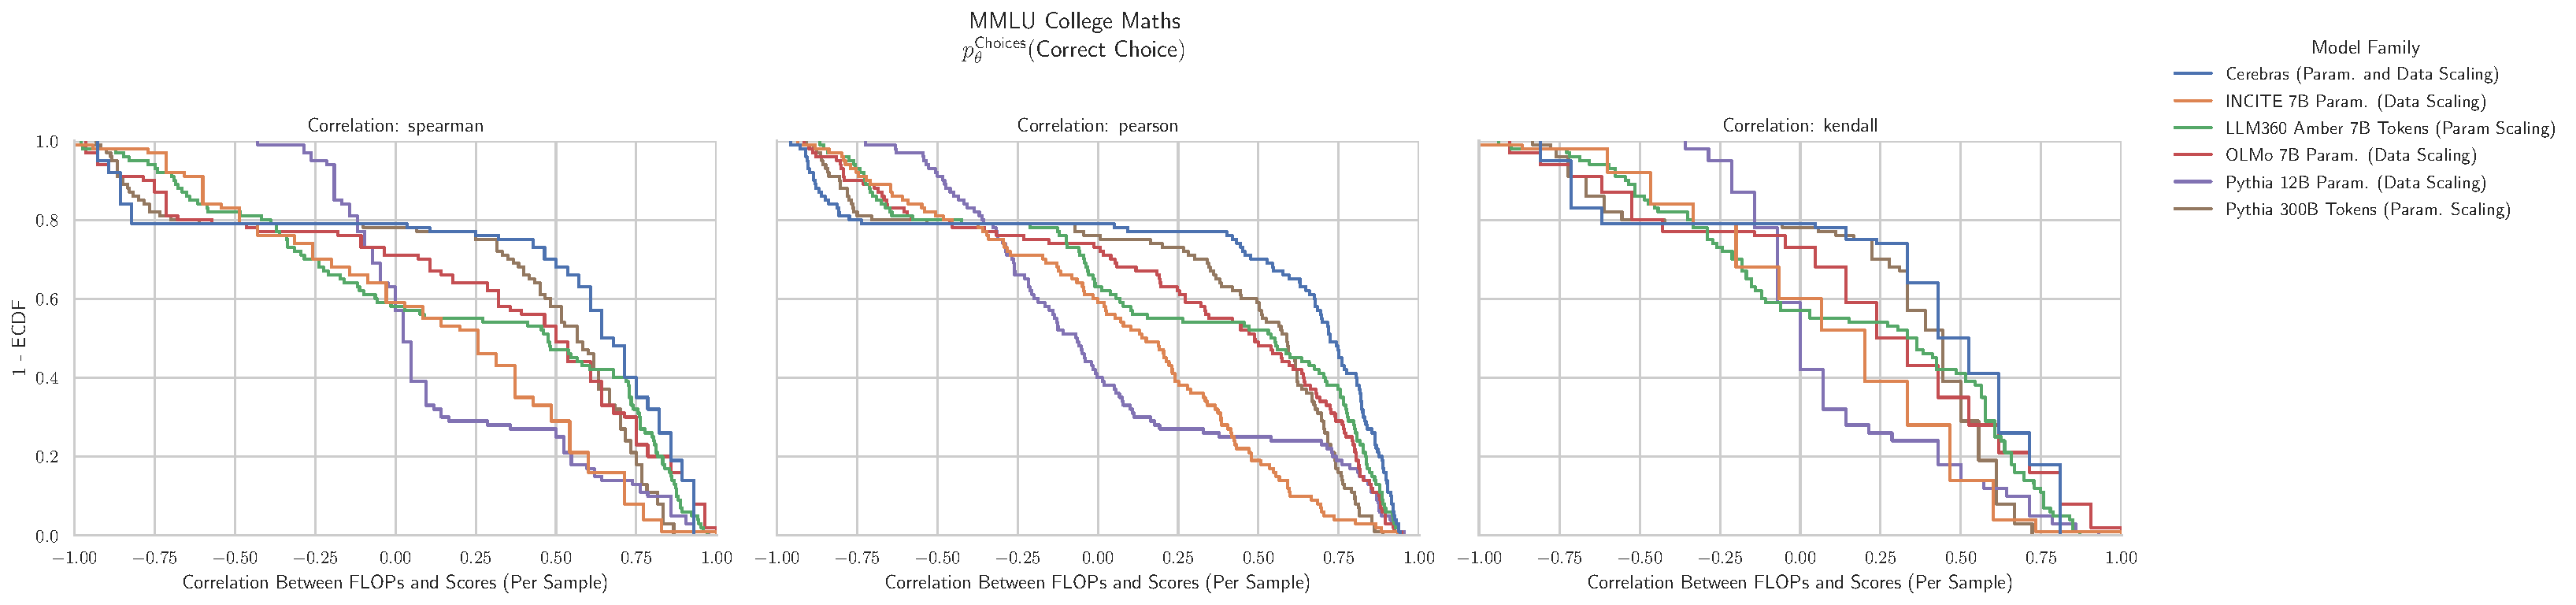
\includegraphics[width=\textwidth]{figures/correlations_between_scores_and_compute/correlation_distributions/mmlu_college_mathematics/mmlu_college_mathematics_prob_correct_choices_ecdf_vs_correlation_score_by_modelfamily_split_correlation_metric.pdf}
    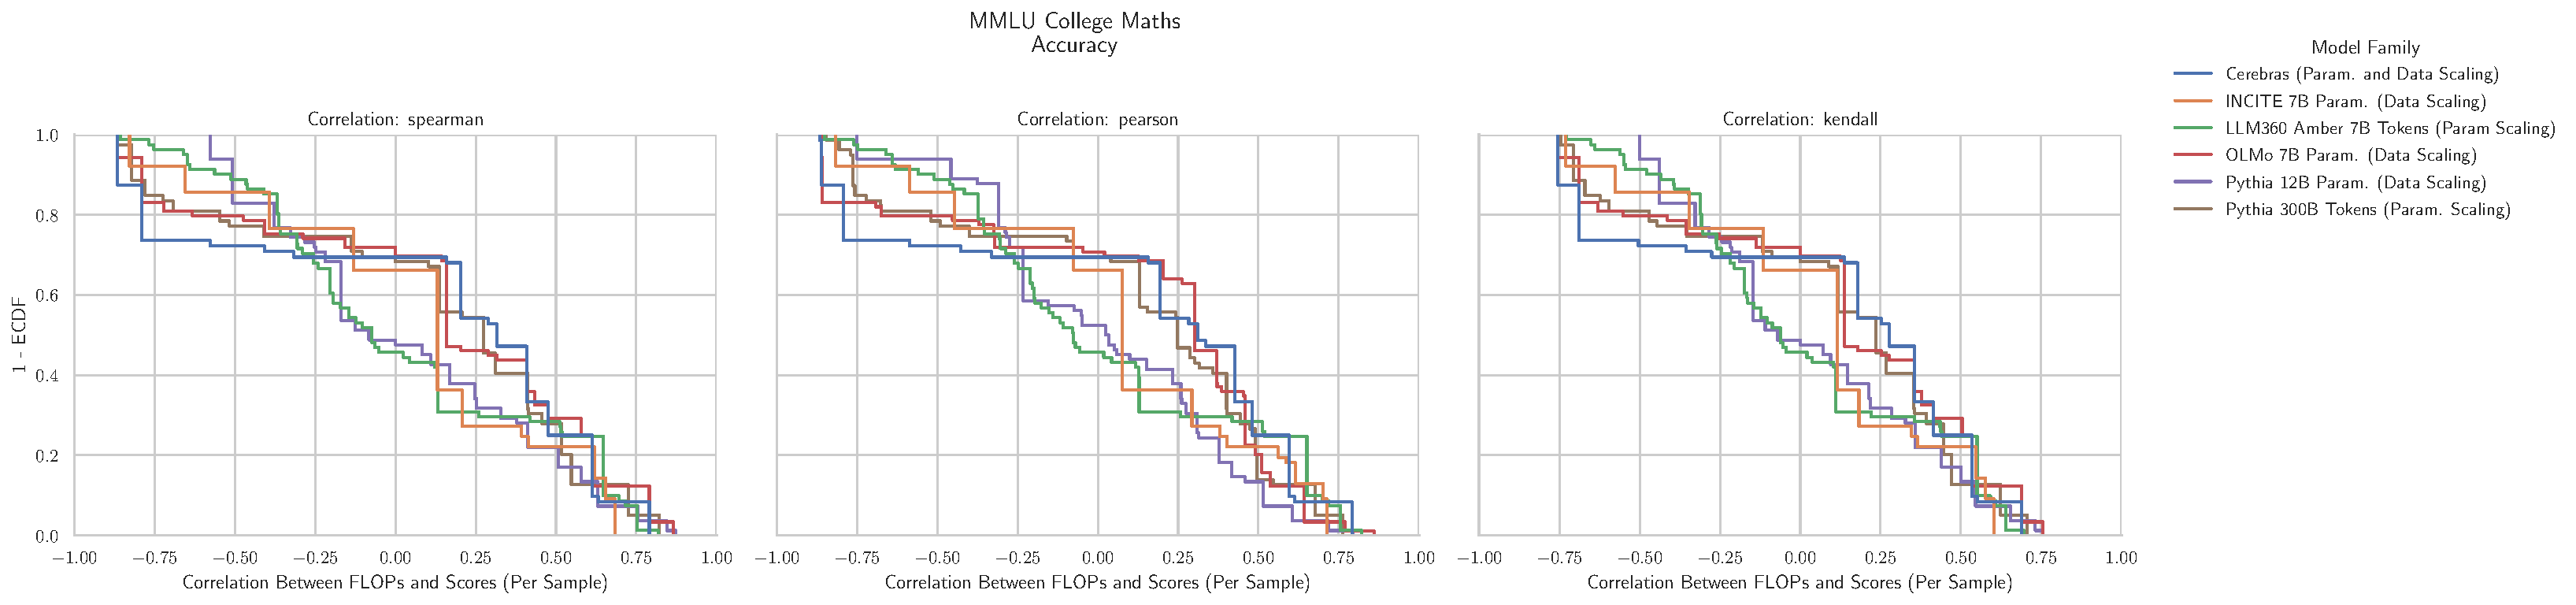
\includegraphics[width=\textwidth]{figures/correlations_between_scores_and_compute/correlation_distributions/mmlu_college_mathematics/mmlu_college_mathematics_acc_ecdf_vs_correlation_score_by_modelfamily_split_correlation_metric.pdf}
    \caption{\textbf{MMLU College Mathematics: Downstream performance is computed via a sequence of transformations that deteriorate correlations between scores and pretraining compute.}}
    \label{app:fig:compute_score_distribution_mmlu_college_mathematics}
\end{figure}


\clearpage
\subsection{NLP Benchmark: MMLU College Medicine \cite{hendrycks2020mmlu}}

\begin{figure}[h!]
    \centering
    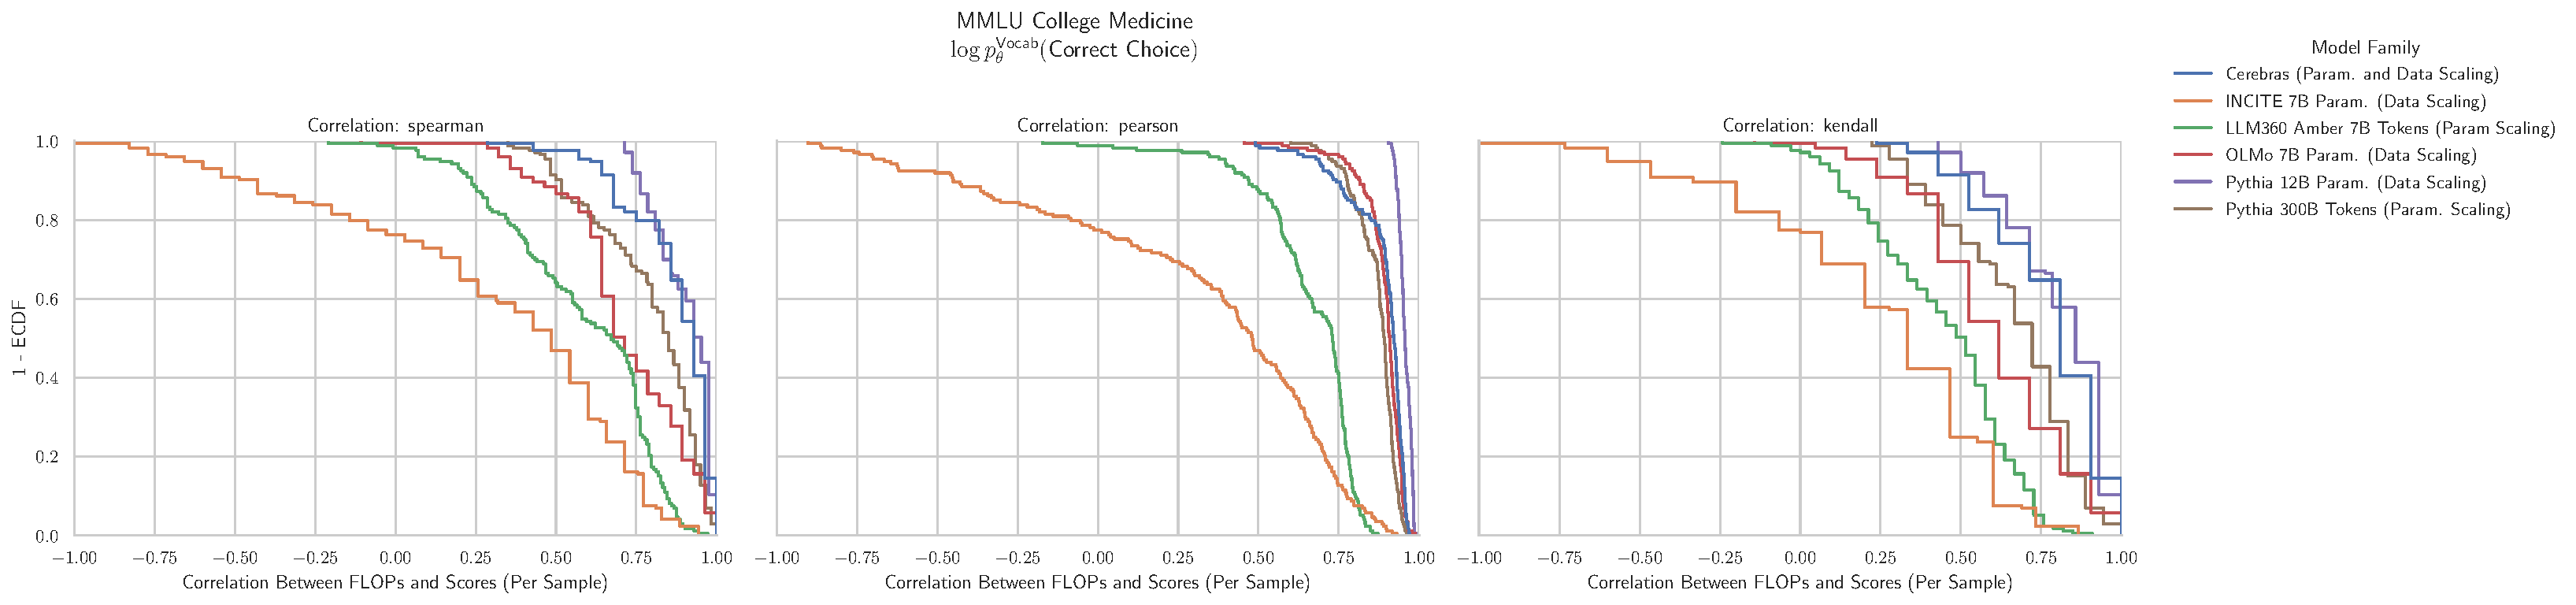
\includegraphics[width=\textwidth]{figures/correlations_between_scores_and_compute/correlation_distributions/mmlu_college_medicine/mmlu_college_medicine_log_likelihood_correct_ecdf_vs_correlation_score_by_modelfamily_split_correlation_metric.pdf}
    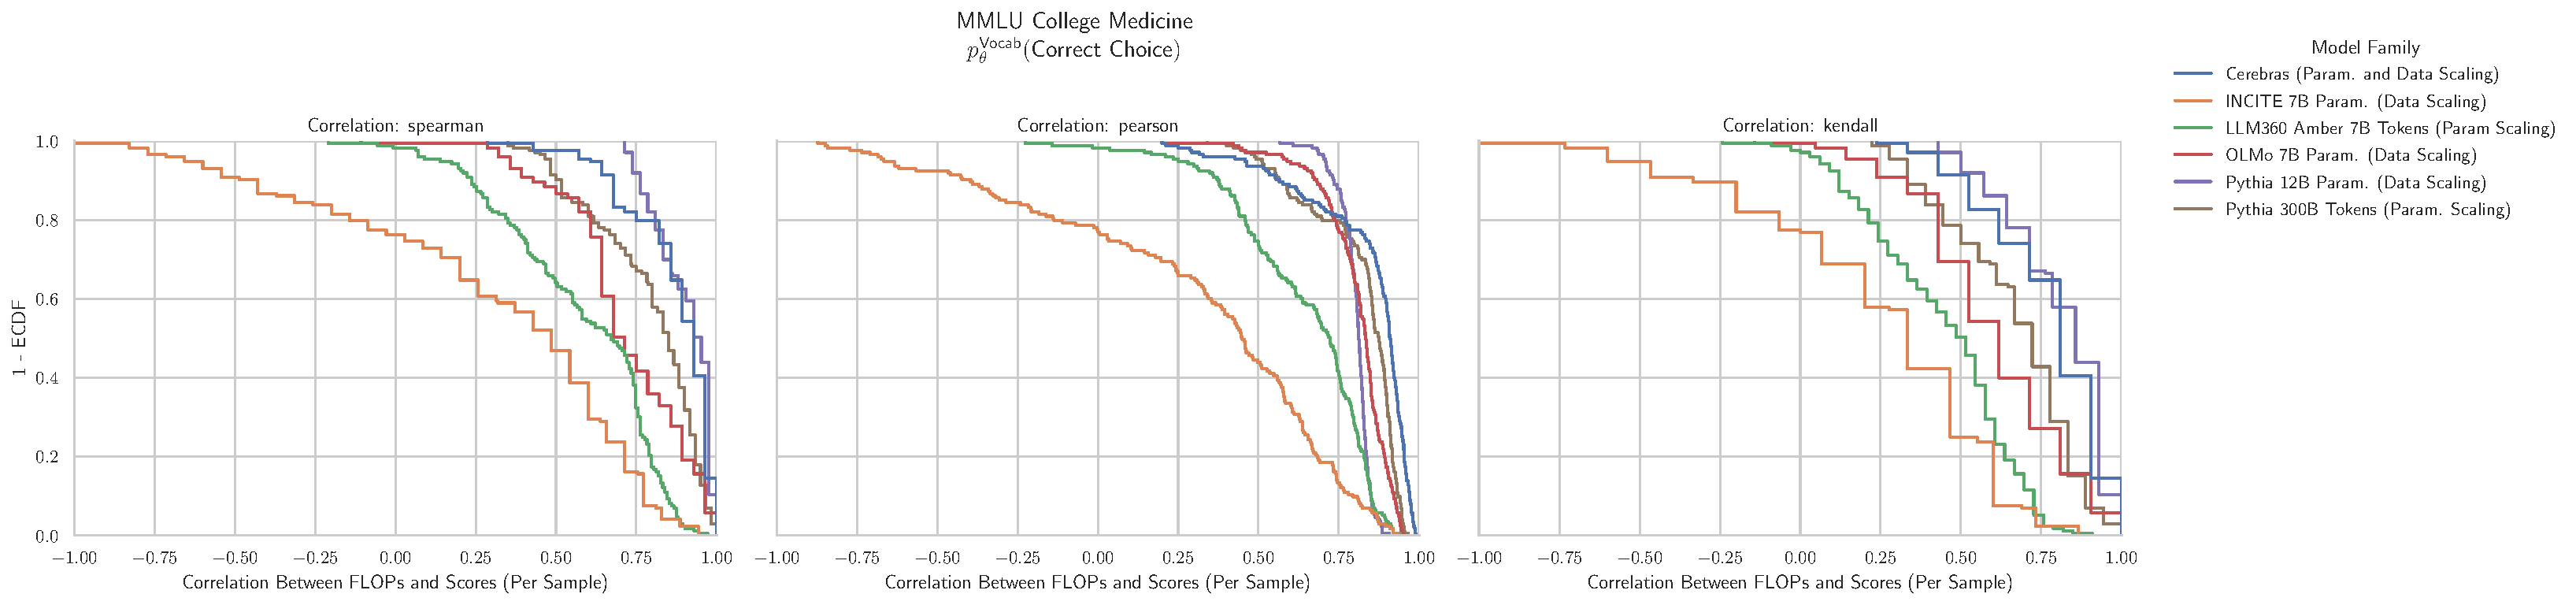
\includegraphics[width=\textwidth]{figures/correlations_between_scores_and_compute/correlation_distributions/mmlu_college_medicine/mmlu_college_medicine_prob_correct_vocab_ecdf_vs_correlation_score_by_modelfamily_split_correlation_metric.pdf}
    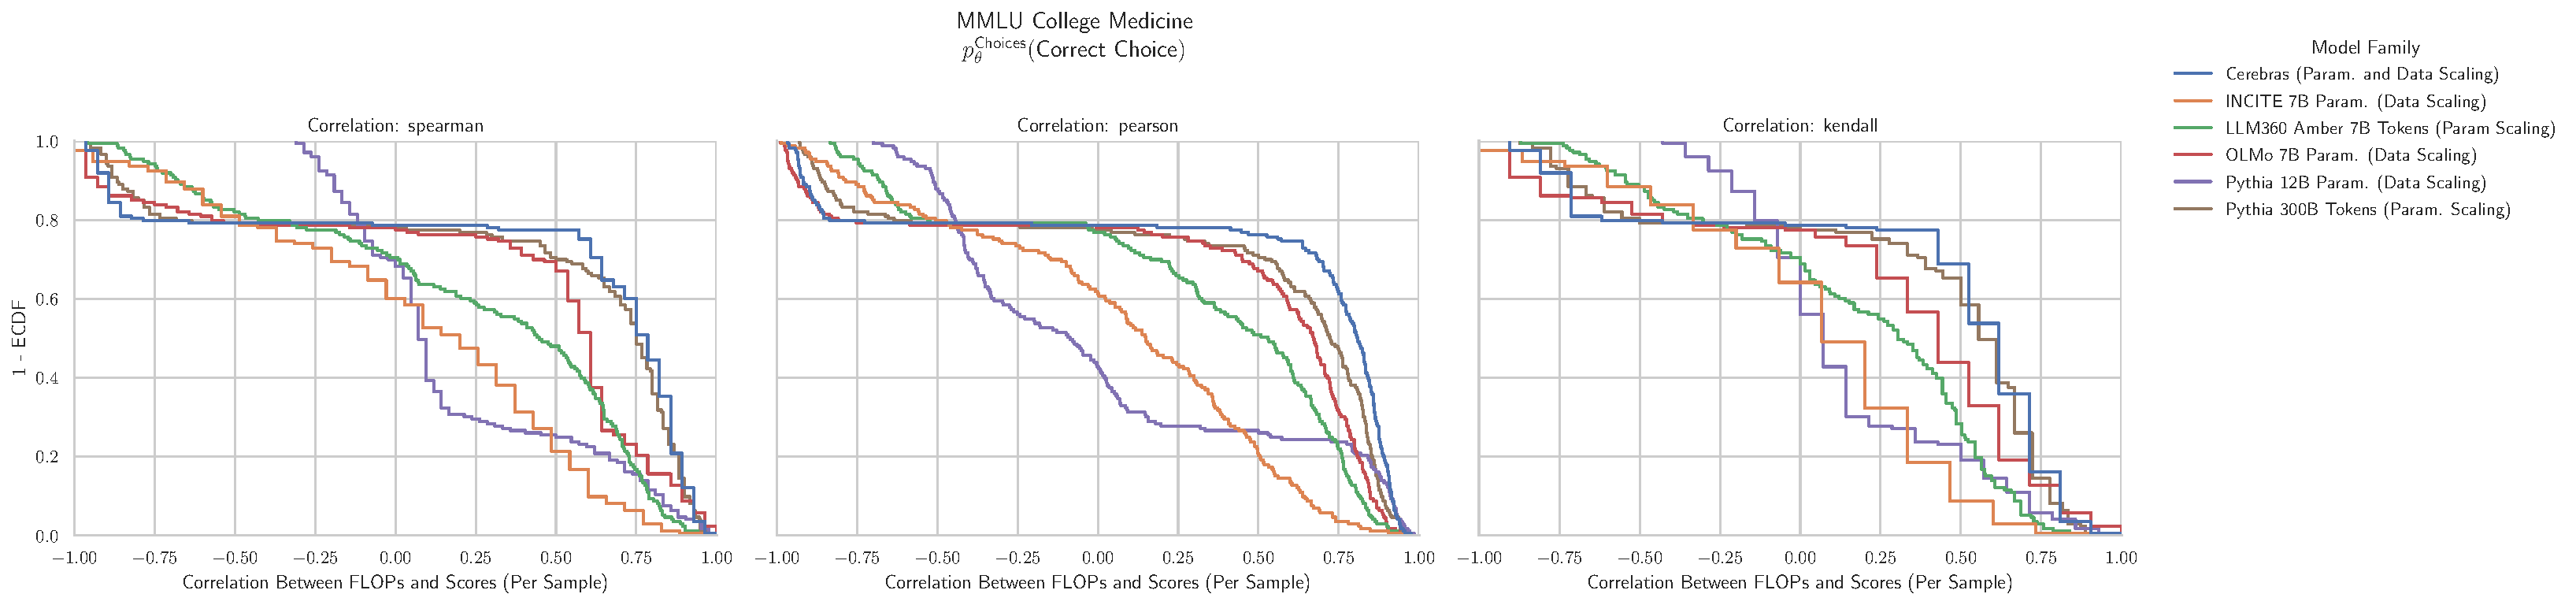
\includegraphics[width=\textwidth]{figures/correlations_between_scores_and_compute/correlation_distributions/mmlu_college_medicine/mmlu_college_medicine_prob_correct_choices_ecdf_vs_correlation_score_by_modelfamily_split_correlation_metric.pdf}
    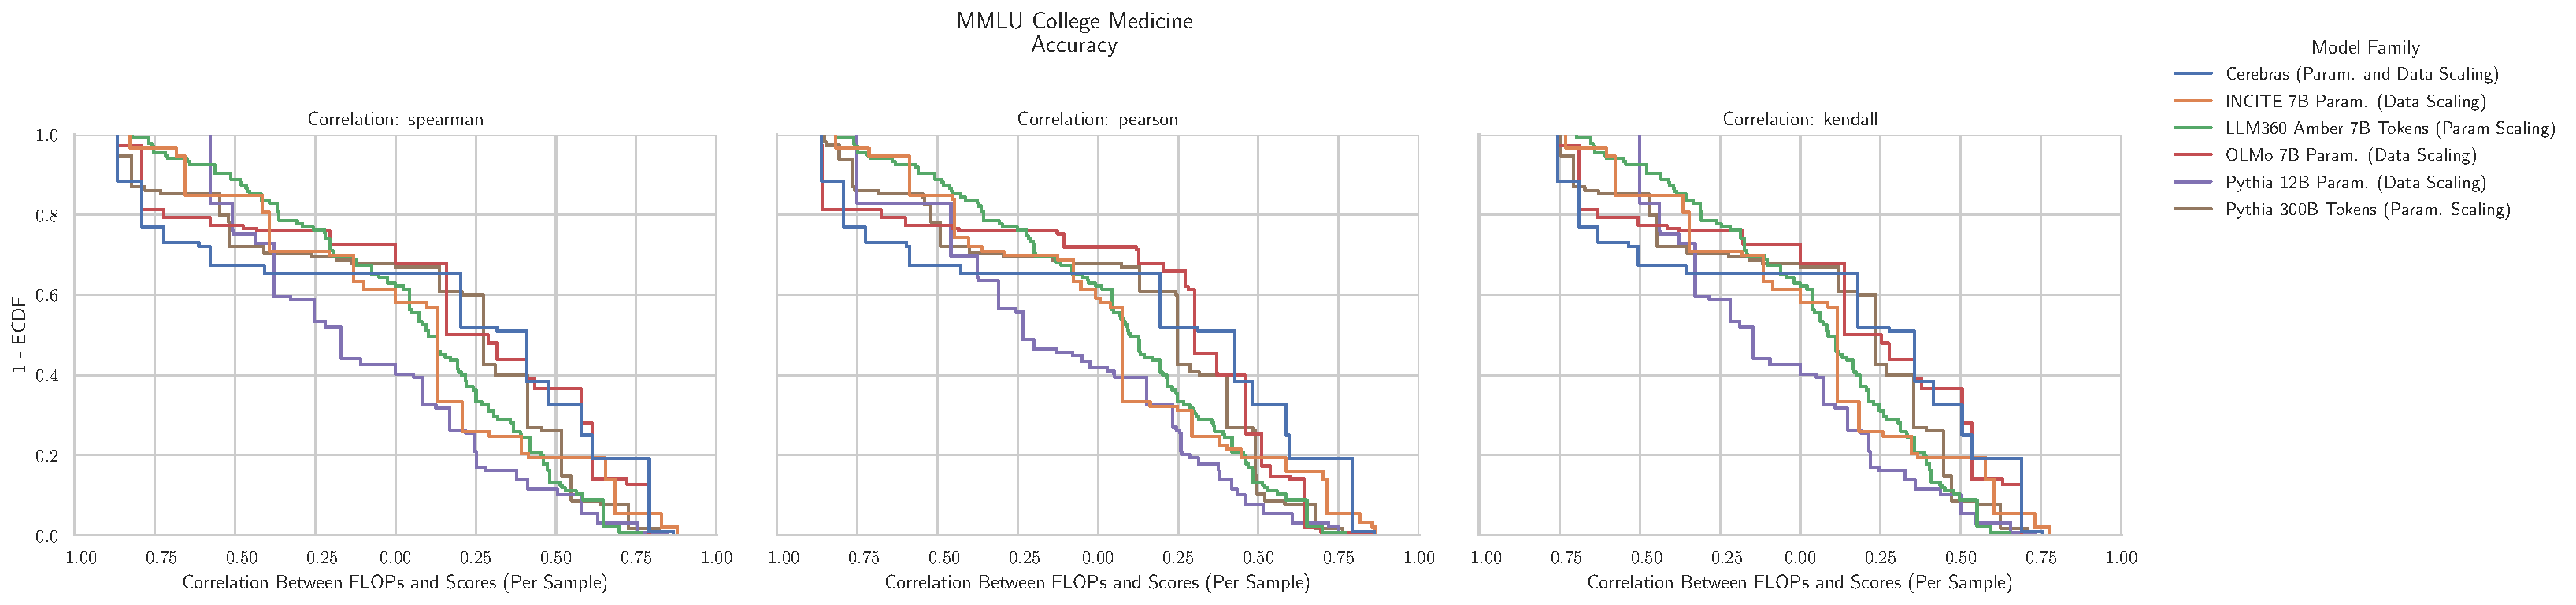
\includegraphics[width=\textwidth]{figures/correlations_between_scores_and_compute/correlation_distributions/mmlu_college_medicine/mmlu_college_medicine_acc_ecdf_vs_correlation_score_by_modelfamily_split_correlation_metric.pdf}
    \caption{\textbf{MMLU College Medicine: Downstream performance is computed via a sequence of transformations that deteriorate correlations between scores and pretraining compute.}}
    \label{app:fig:compute_score_distribution_mmlu_college_medicine}
\end{figure}


\clearpage
\subsection{NLP Benchmark: MMLU College Physics \cite{hendrycks2020mmlu}}

\begin{figure}[h!]
    \centering
    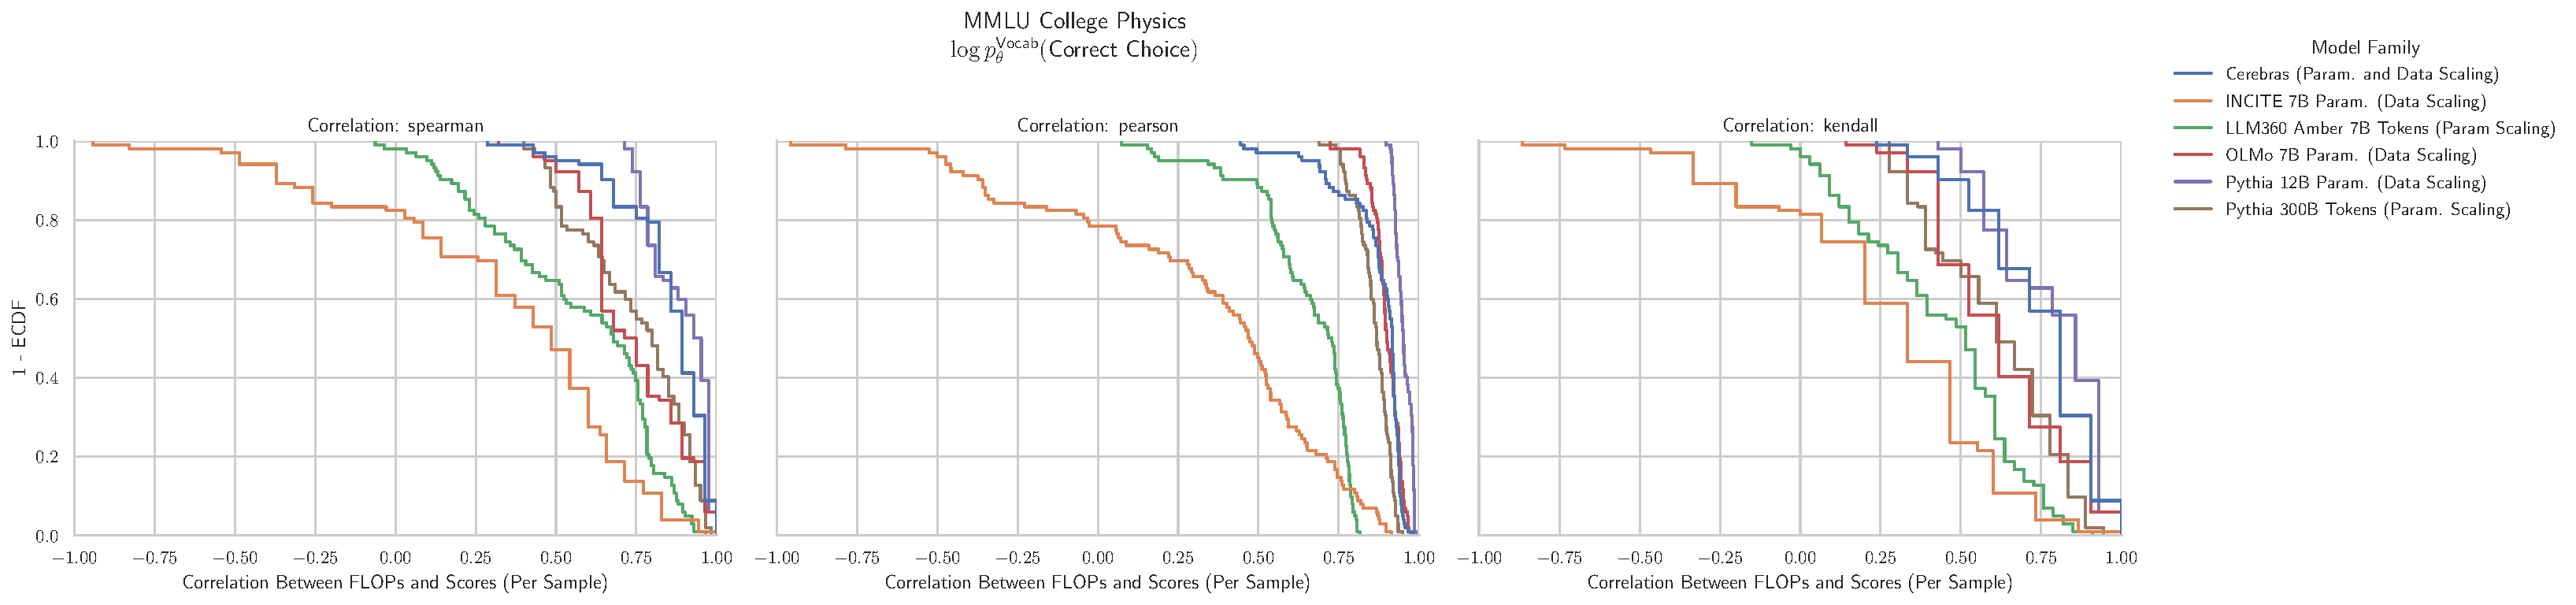
\includegraphics[width=\textwidth]{figures/correlations_between_scores_and_compute/correlation_distributions/mmlu_college_physics/mmlu_college_physics_log_likelihood_correct_ecdf_vs_correlation_score_by_modelfamily_split_correlation_metric.pdf}
    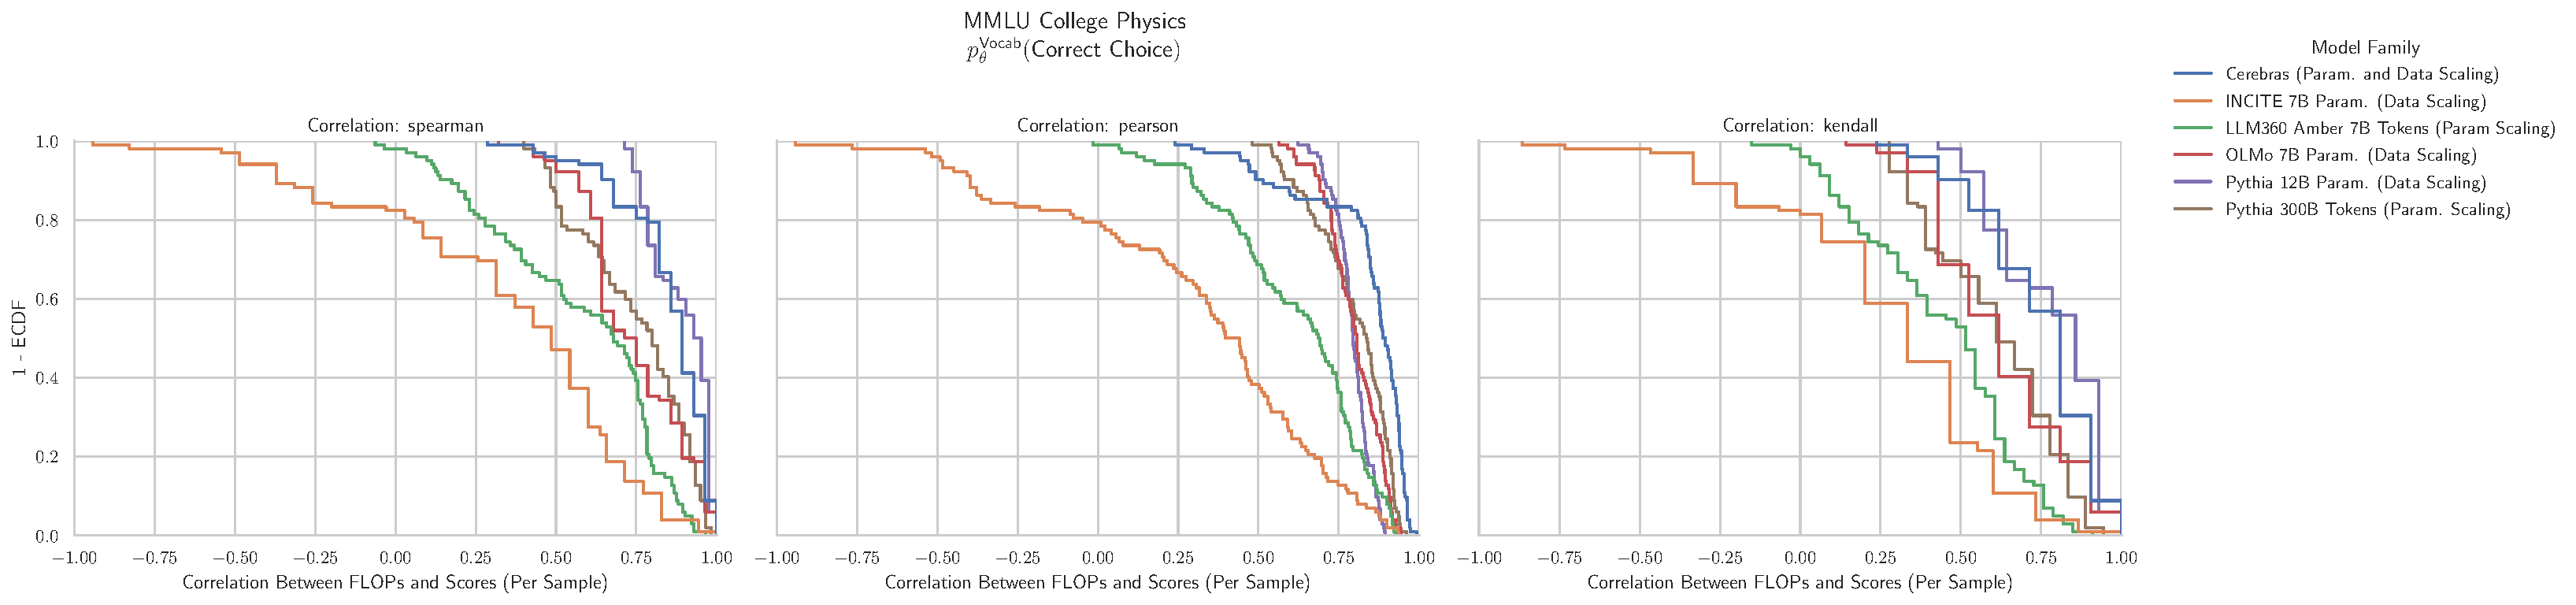
\includegraphics[width=\textwidth]{figures/correlations_between_scores_and_compute/correlation_distributions/mmlu_college_physics/mmlu_college_physics_prob_correct_vocab_ecdf_vs_correlation_score_by_modelfamily_split_correlation_metric.pdf}
    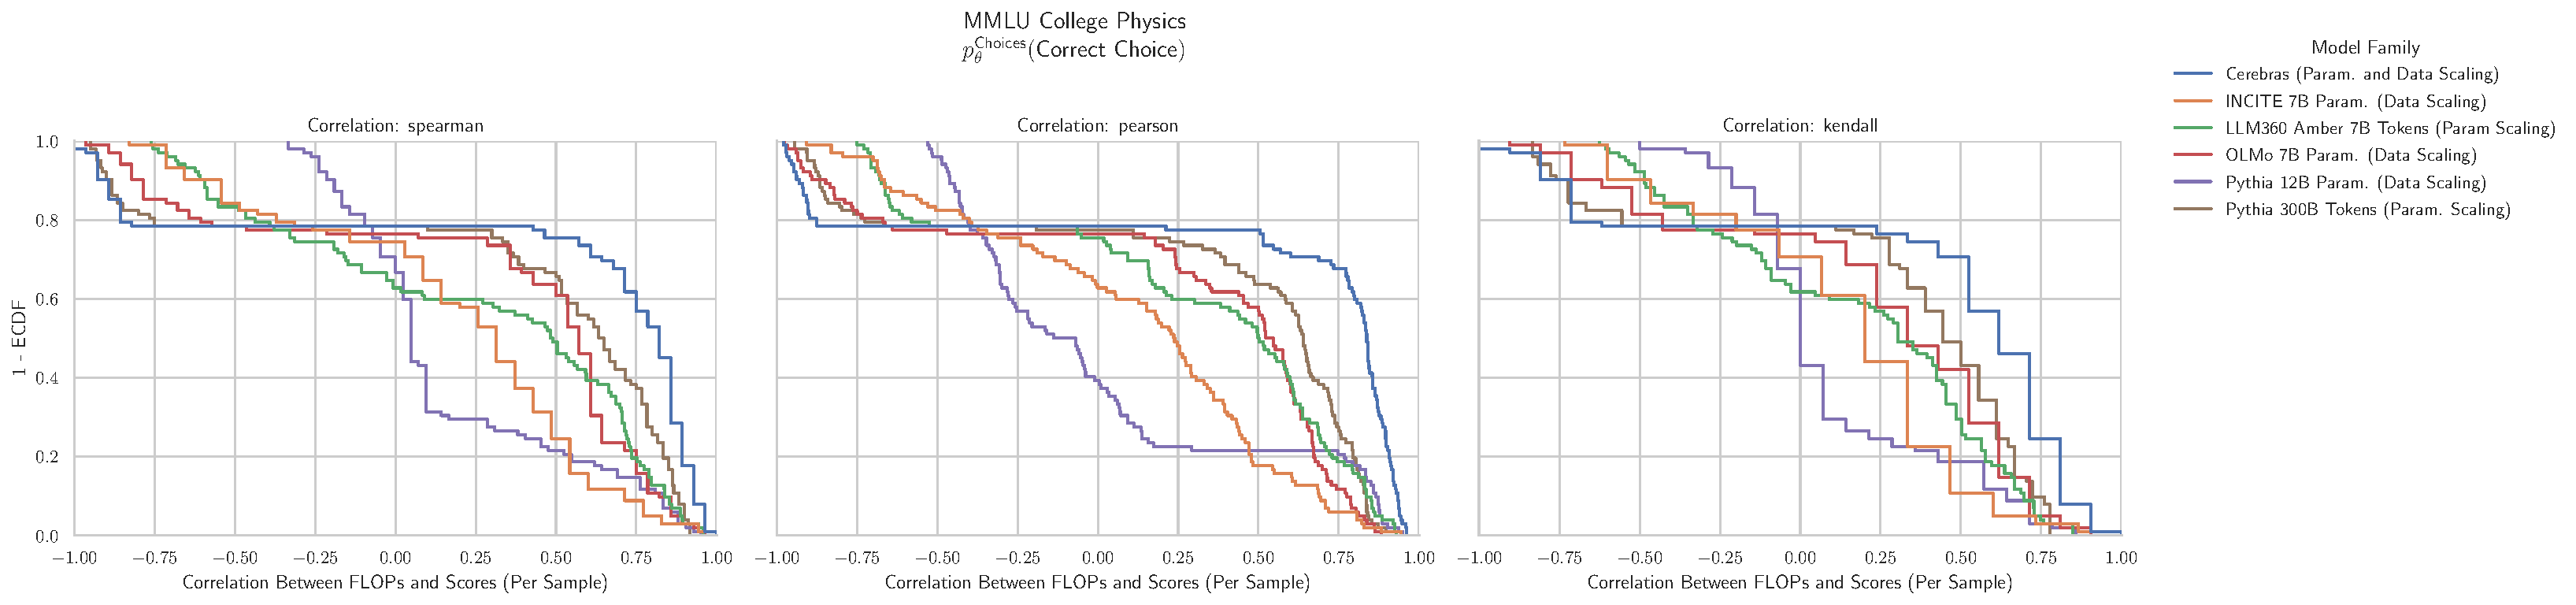
\includegraphics[width=\textwidth]{figures/correlations_between_scores_and_compute/correlation_distributions/mmlu_college_physics/mmlu_college_physics_prob_correct_choices_ecdf_vs_correlation_score_by_modelfamily_split_correlation_metric.pdf}
    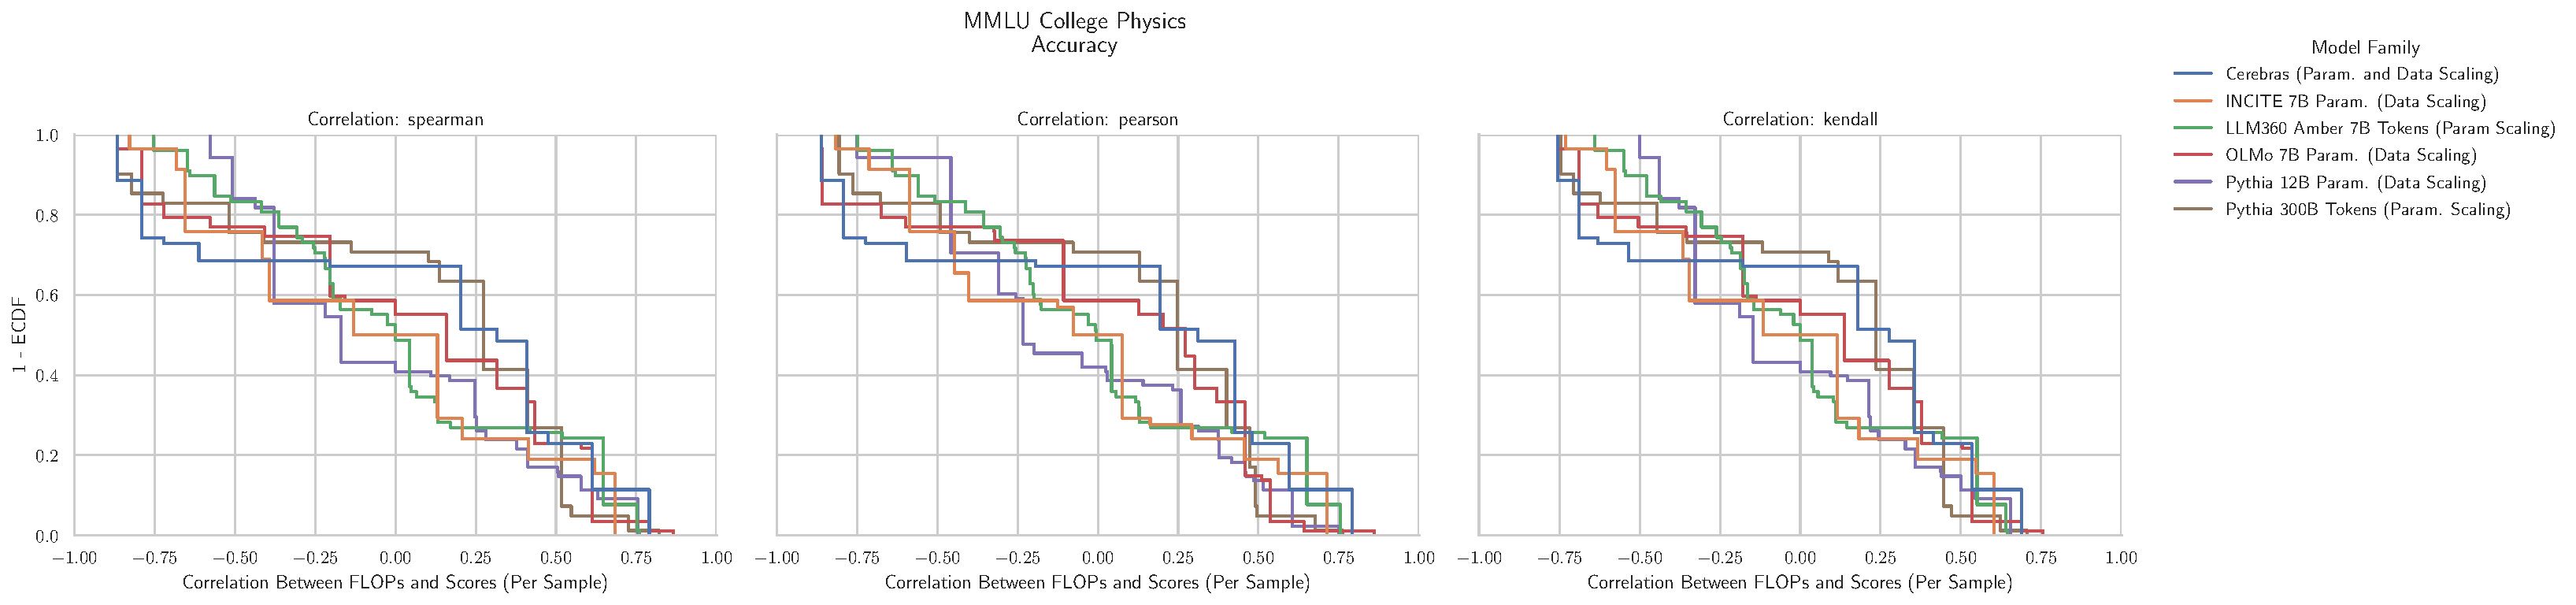
\includegraphics[width=\textwidth]{figures/correlations_between_scores_and_compute/correlation_distributions/mmlu_college_physics/mmlu_college_physics_acc_ecdf_vs_correlation_score_by_modelfamily_split_correlation_metric.pdf}
    \caption{\textbf{MMLU College Physics: Downstream performance is computed via a sequence of transformations that deteriorate correlations between scores and pretraining compute.}}
    \label{app:fig:compute_score_distribution_mmlu_college_physics}
\end{figure}


\clearpage
\subsection{NLP Benchmark: MMLU Computer Security \cite{hendrycks2020mmlu}}

\begin{figure}[h!]
    \centering
    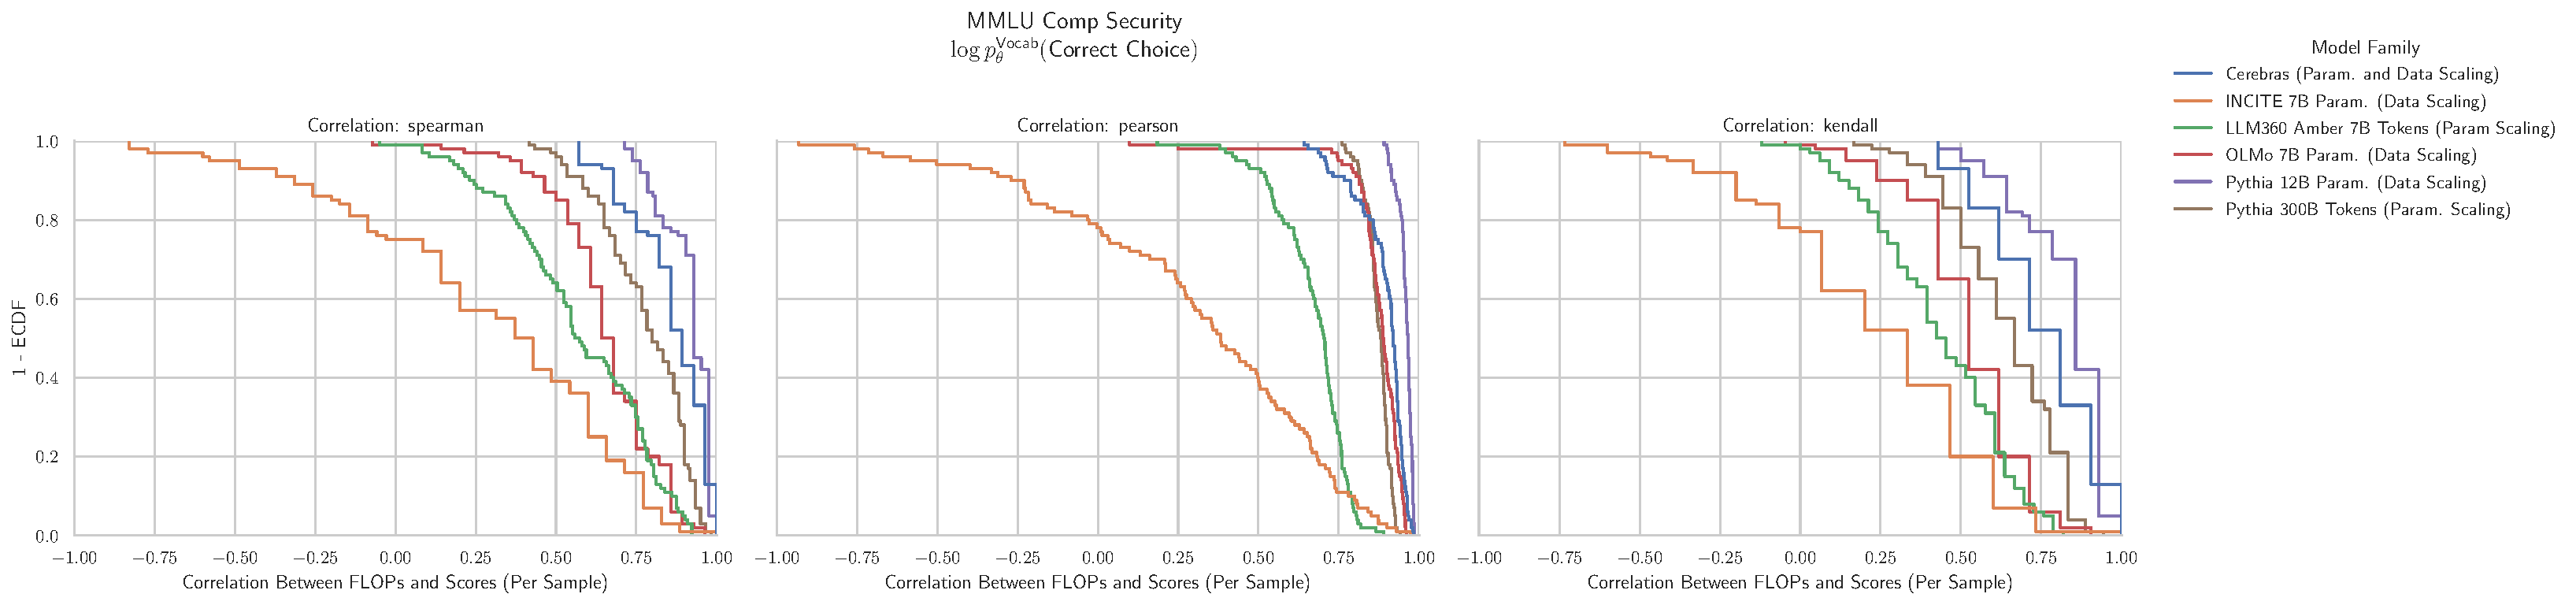
\includegraphics[width=\textwidth]{figures/correlations_between_scores_and_compute/correlation_distributions/mmlu_computer_security/mmlu_computer_security_log_likelihood_correct_ecdf_vs_correlation_score_by_modelfamily_split_correlation_metric.pdf}
    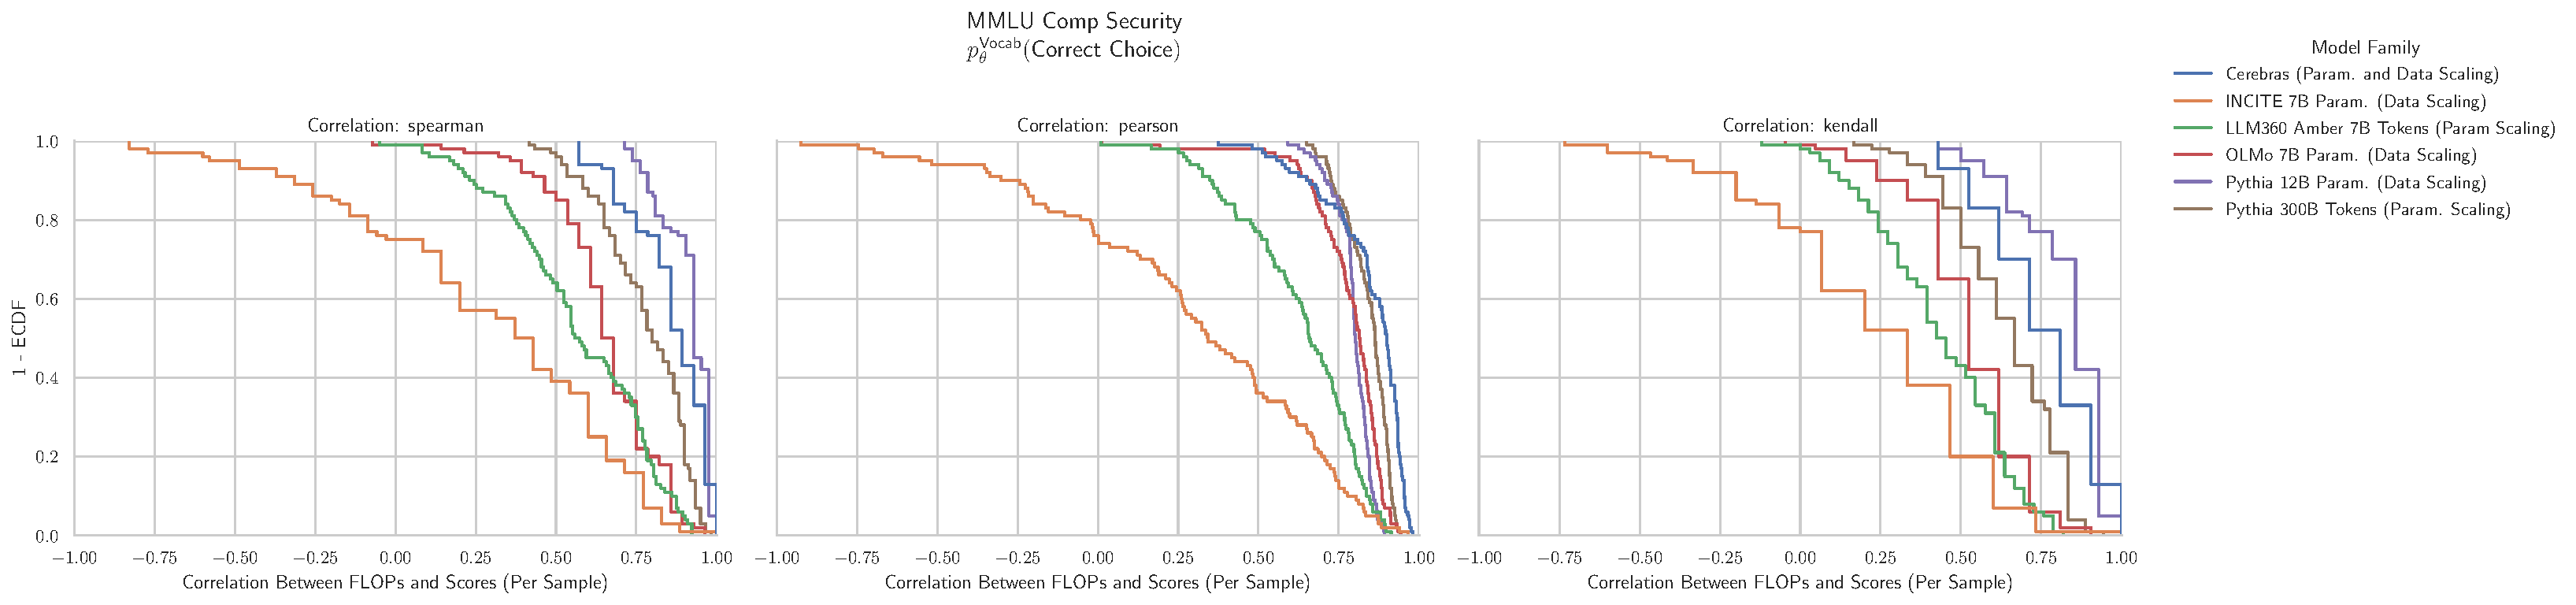
\includegraphics[width=\textwidth]{figures/correlations_between_scores_and_compute/correlation_distributions/mmlu_computer_security/mmlu_computer_security_prob_correct_vocab_ecdf_vs_correlation_score_by_modelfamily_split_correlation_metric.pdf}
    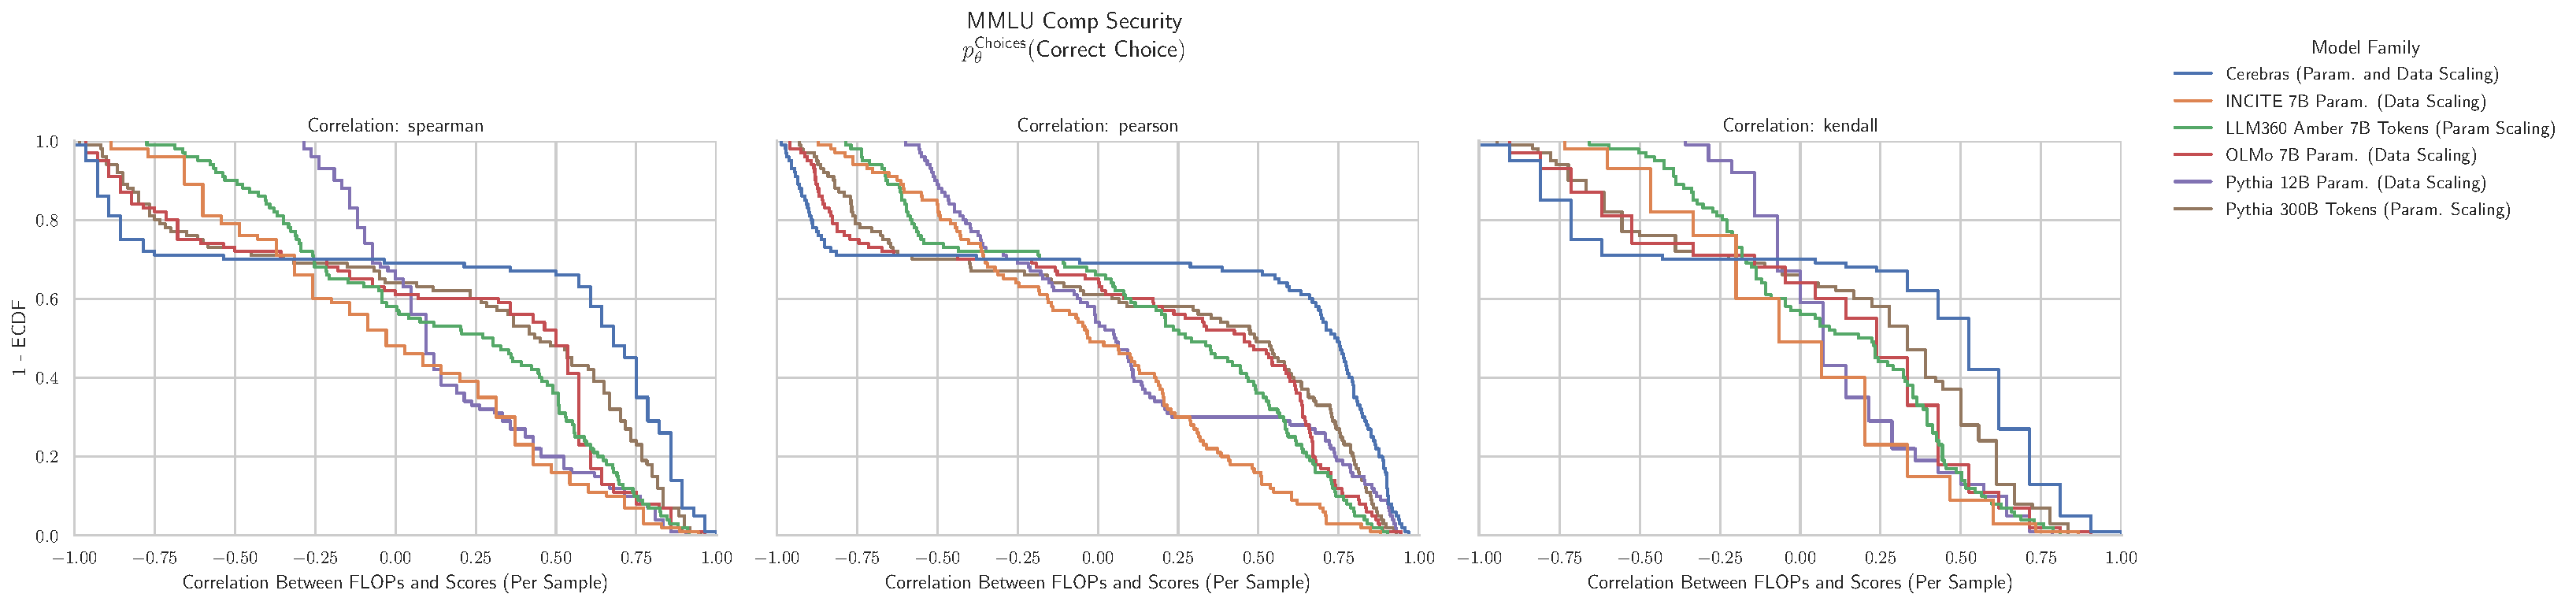
\includegraphics[width=\textwidth]{figures/correlations_between_scores_and_compute/correlation_distributions/mmlu_computer_security/mmlu_computer_security_prob_correct_choices_ecdf_vs_correlation_score_by_modelfamily_split_correlation_metric.pdf}
    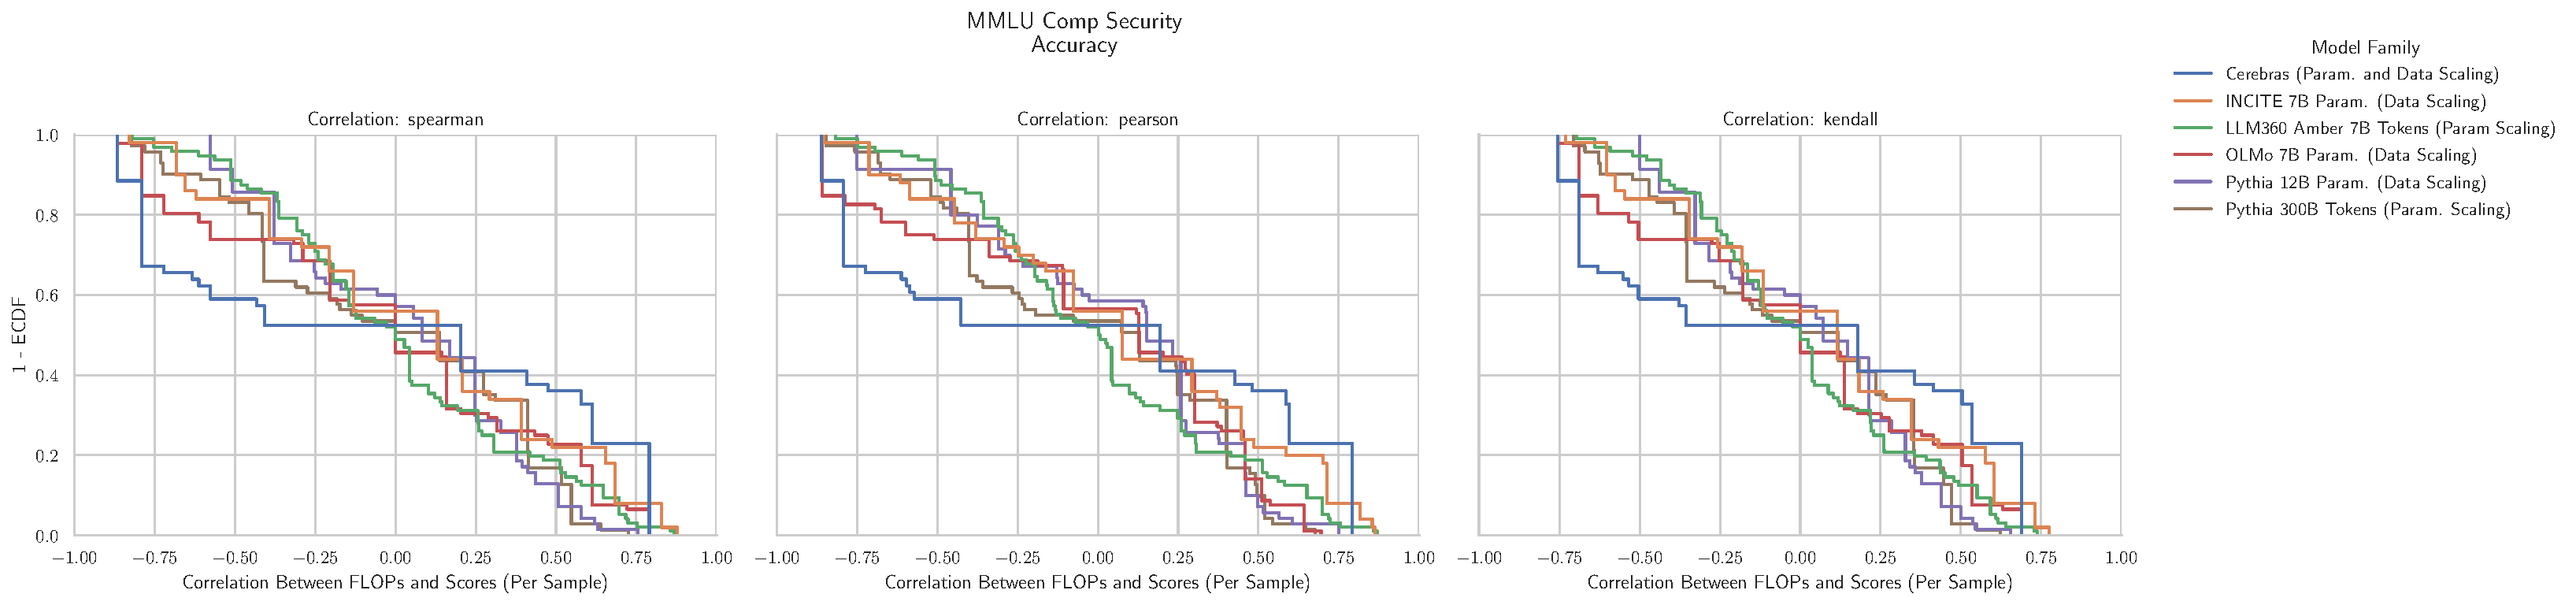
\includegraphics[width=\textwidth]{figures/correlations_between_scores_and_compute/correlation_distributions/mmlu_computer_security/mmlu_computer_security_acc_ecdf_vs_correlation_score_by_modelfamily_split_correlation_metric.pdf}
    \caption{\textbf{MMLU Computer Security: Downstream performance is computed via a sequence of transformations that deteriorate correlations between scores and pretraining compute.}}
    \label{app:fig:compute_score_distribution_mmlu_computer_security}
\end{figure}


\clearpage
\subsection{NLP Benchmark: MMLU Conceptual Physics \cite{hendrycks2020mmlu}}

\begin{figure}[h!]
    \centering
    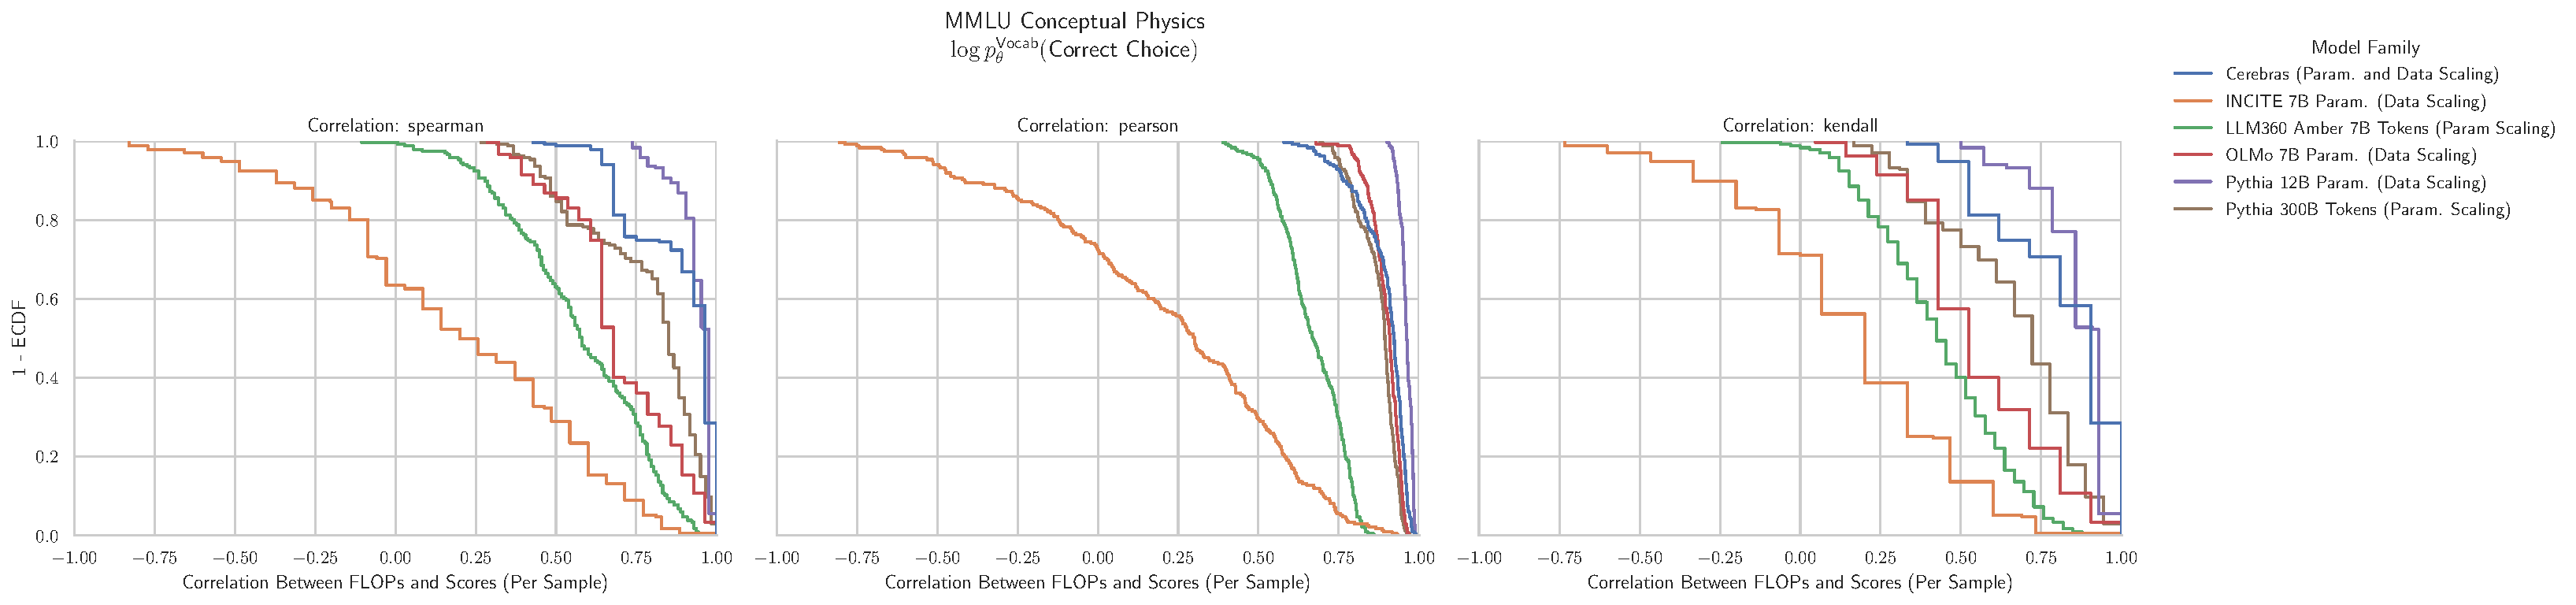
\includegraphics[width=\textwidth]{figures/correlations_between_scores_and_compute/correlation_distributions/mmlu_conceptual_physics/mmlu_conceptual_physics_log_likelihood_correct_ecdf_vs_correlation_score_by_modelfamily_split_correlation_metric.pdf}
    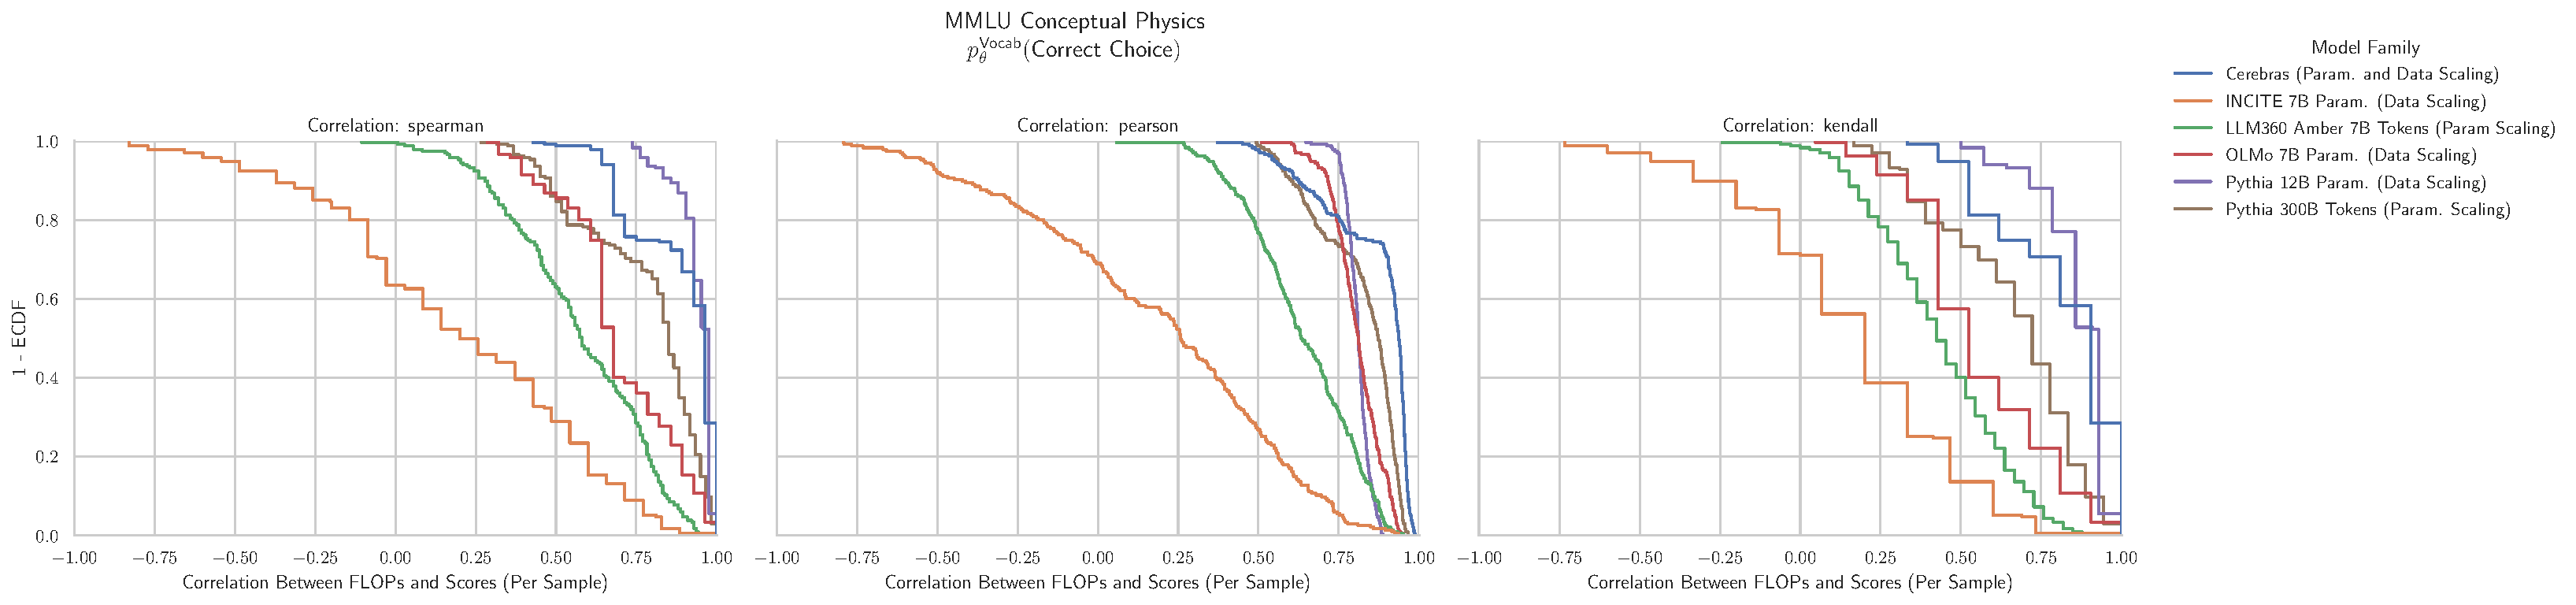
\includegraphics[width=\textwidth]{figures/correlations_between_scores_and_compute/correlation_distributions/mmlu_conceptual_physics/mmlu_conceptual_physics_prob_correct_vocab_ecdf_vs_correlation_score_by_modelfamily_split_correlation_metric.pdf}
    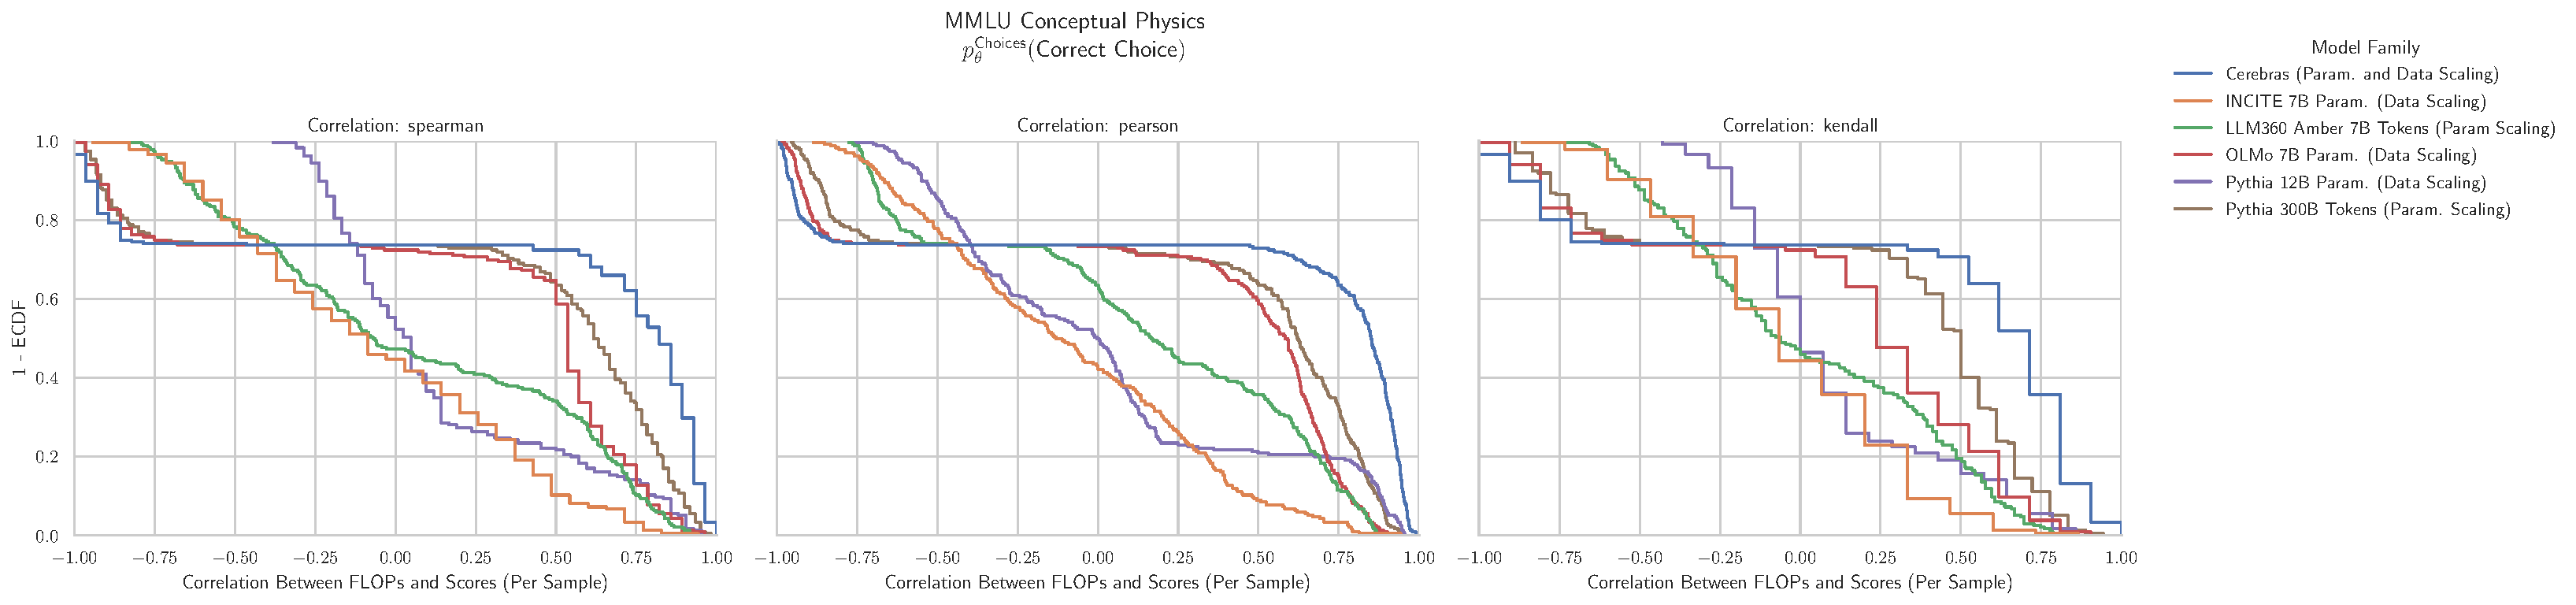
\includegraphics[width=\textwidth]{figures/correlations_between_scores_and_compute/correlation_distributions/mmlu_conceptual_physics/mmlu_conceptual_physics_prob_correct_choices_ecdf_vs_correlation_score_by_modelfamily_split_correlation_metric.pdf}
    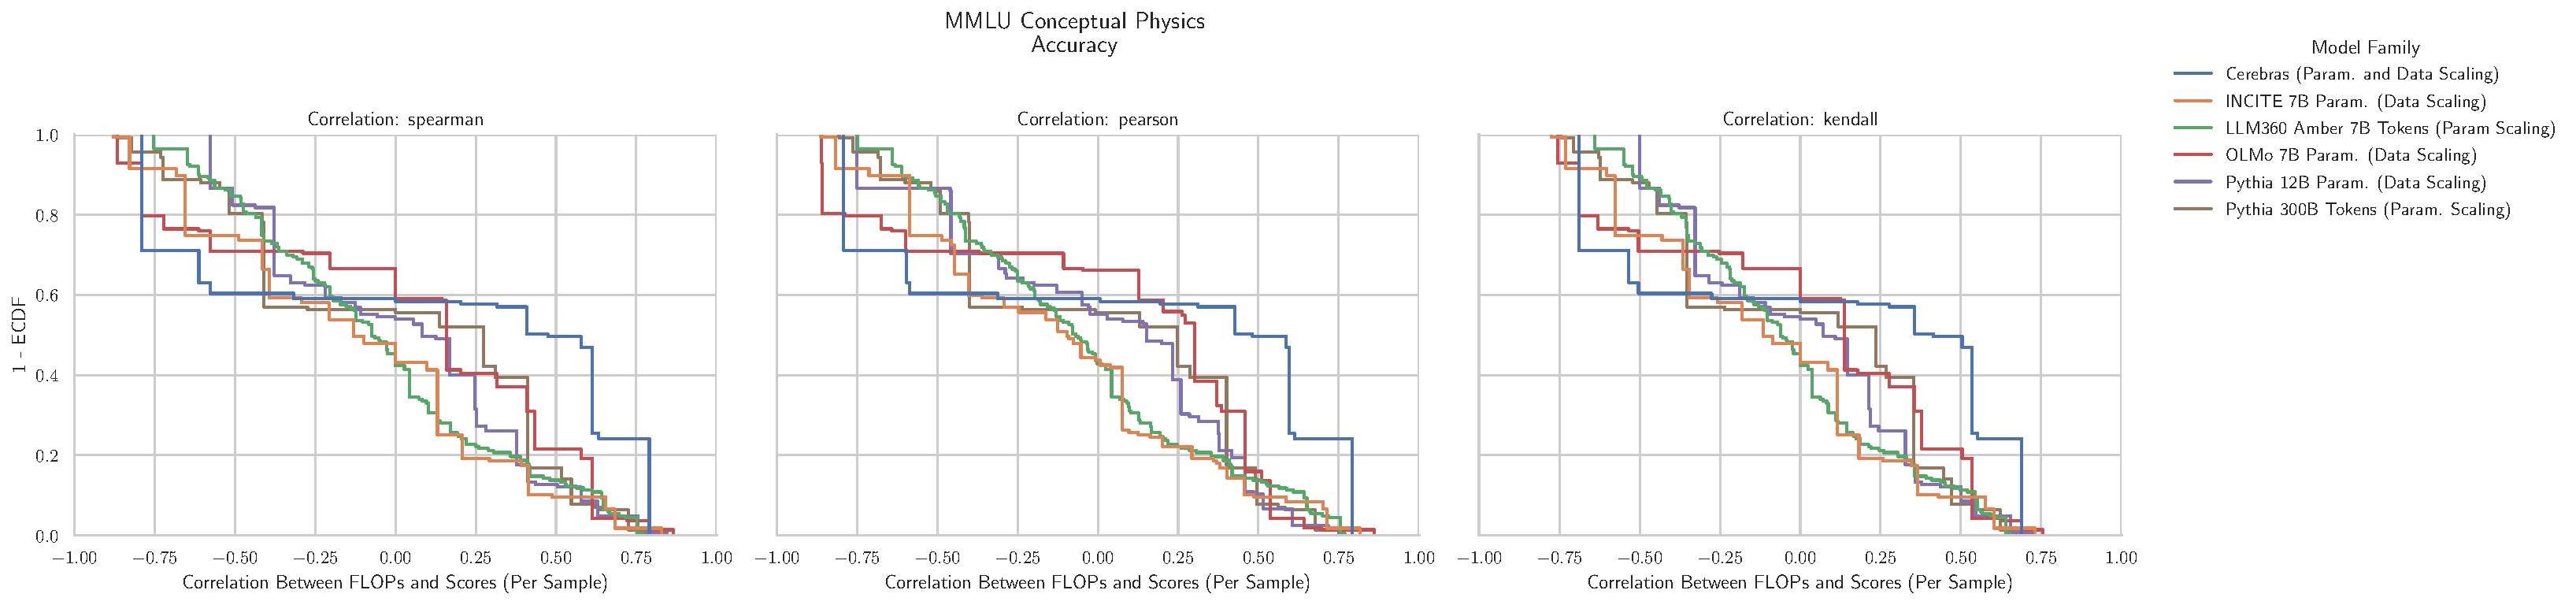
\includegraphics[width=\textwidth]{figures/correlations_between_scores_and_compute/correlation_distributions/mmlu_conceptual_physics/mmlu_conceptual_physics_acc_ecdf_vs_correlation_score_by_modelfamily_split_correlation_metric.pdf}
    \caption{\textbf{MMLU Conceptual Physics: Downstream performance is computed via a sequence of transformations that deteriorate correlations between scores and pretraining compute.}}
    \label{app:fig:compute_score_distribution_mmlu_conceptual_physics}
\end{figure}


\clearpage
\subsection{NLP Benchmark: MMLU Econometrics \cite{hendrycks2020mmlu}}

\begin{figure}[h!]
    \centering
    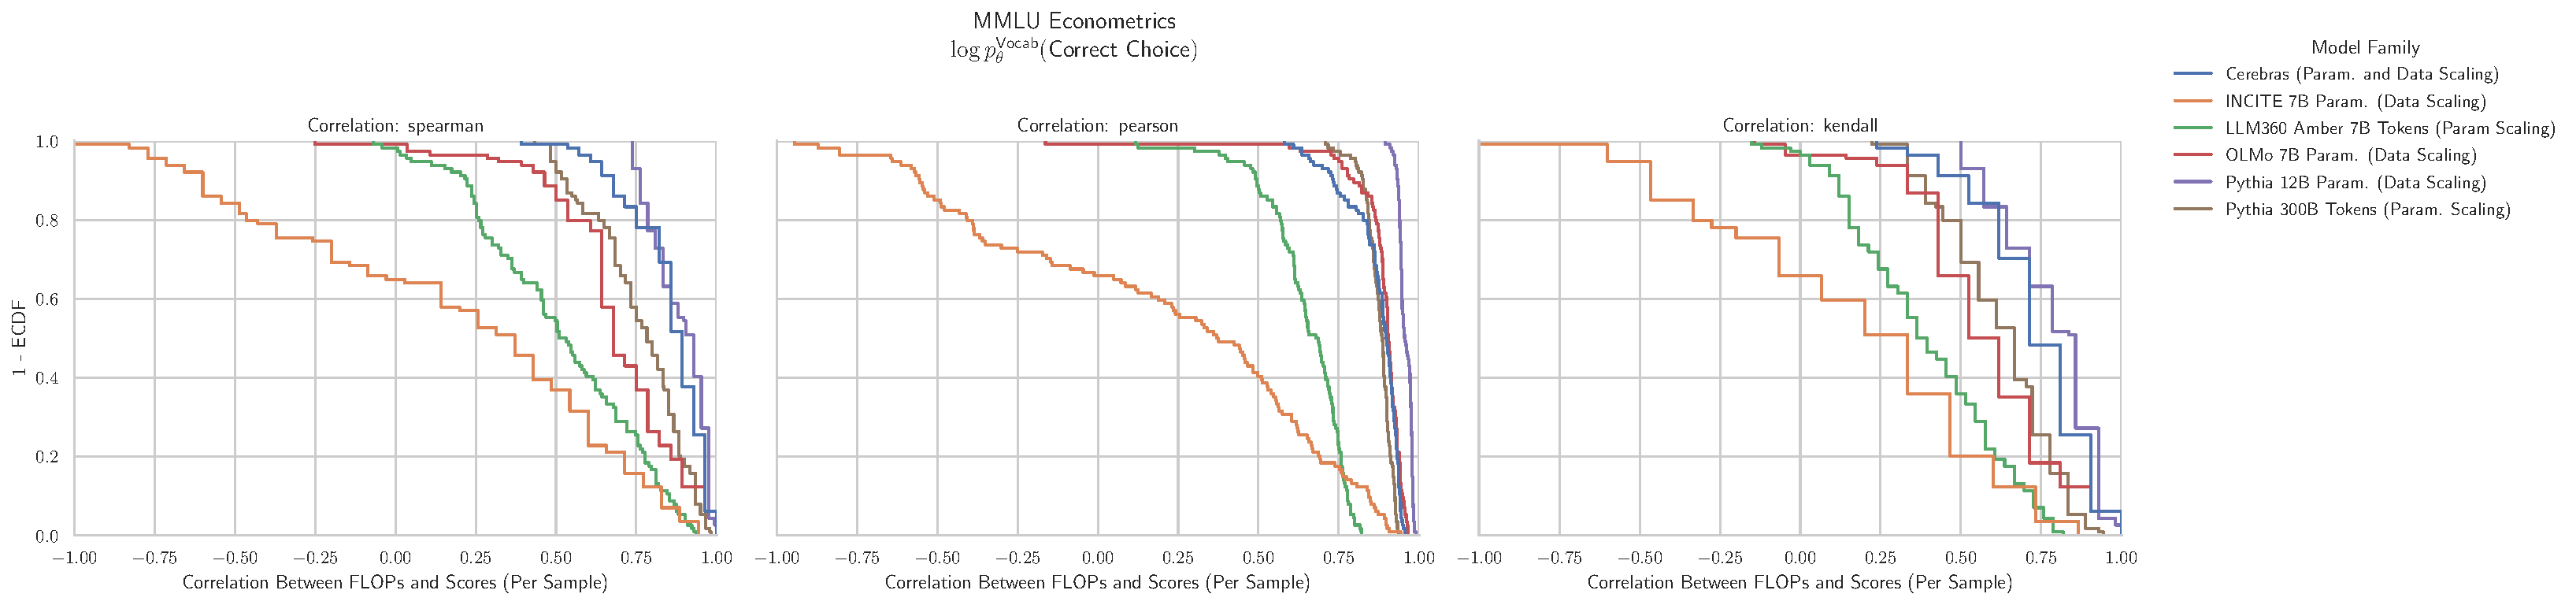
\includegraphics[width=\textwidth]{figures/correlations_between_scores_and_compute/correlation_distributions/mmlu_econometrics/mmlu_econometrics_log_likelihood_correct_ecdf_vs_correlation_score_by_modelfamily_split_correlation_metric.pdf}
    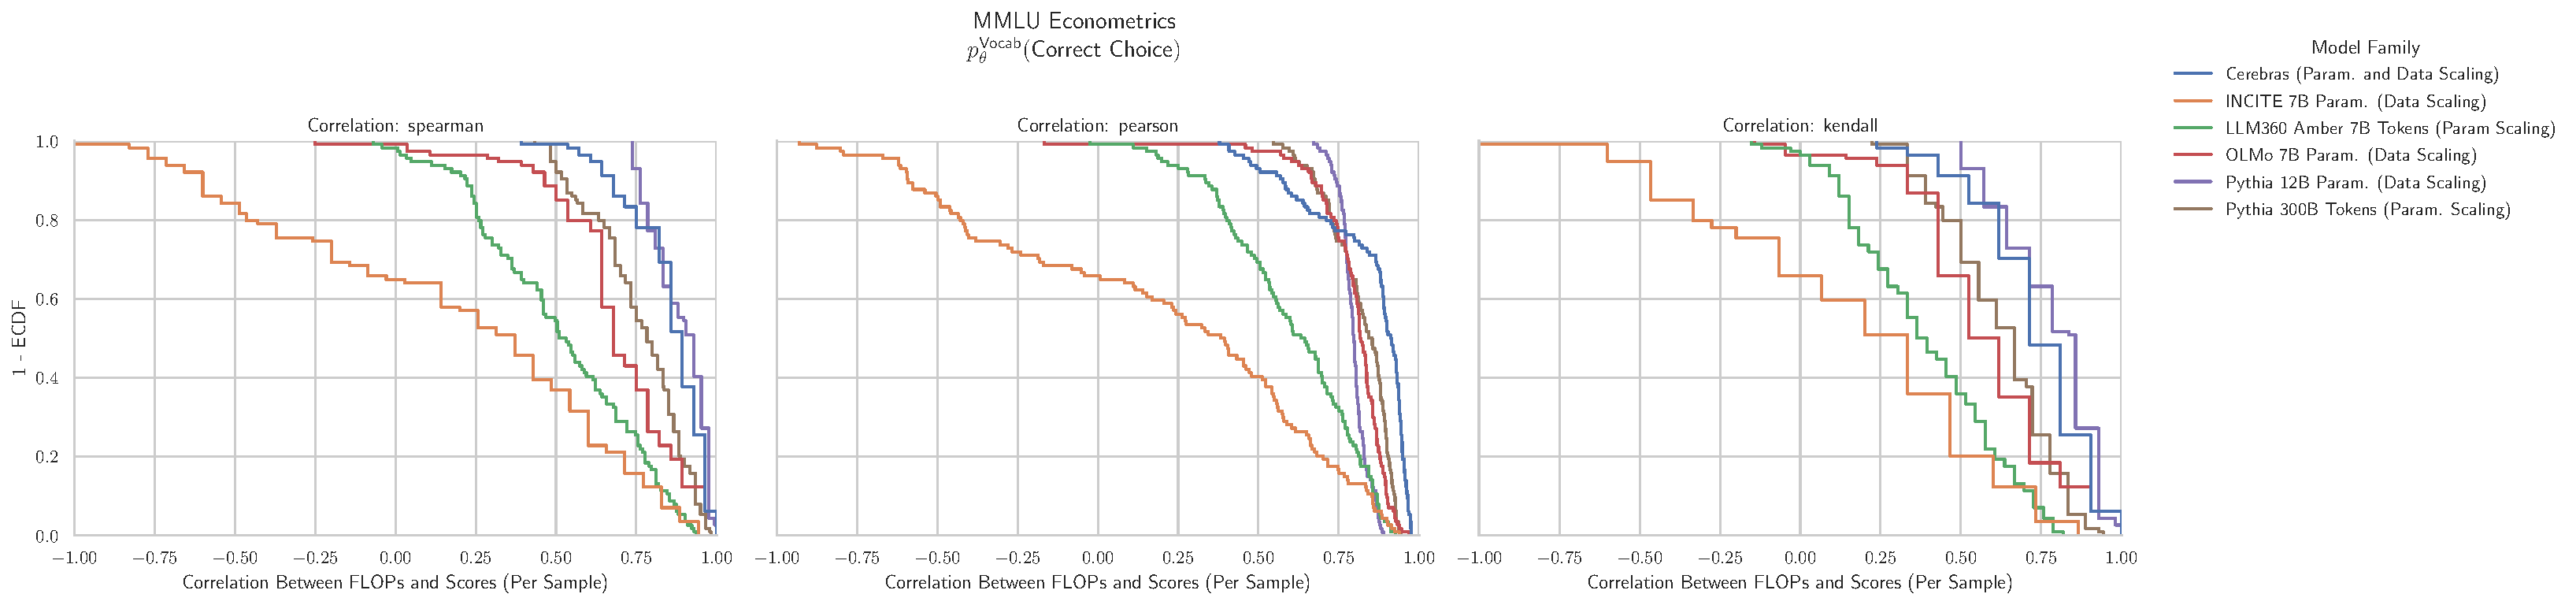
\includegraphics[width=\textwidth]{figures/correlations_between_scores_and_compute/correlation_distributions/mmlu_econometrics/mmlu_econometrics_prob_correct_vocab_ecdf_vs_correlation_score_by_modelfamily_split_correlation_metric.pdf}
    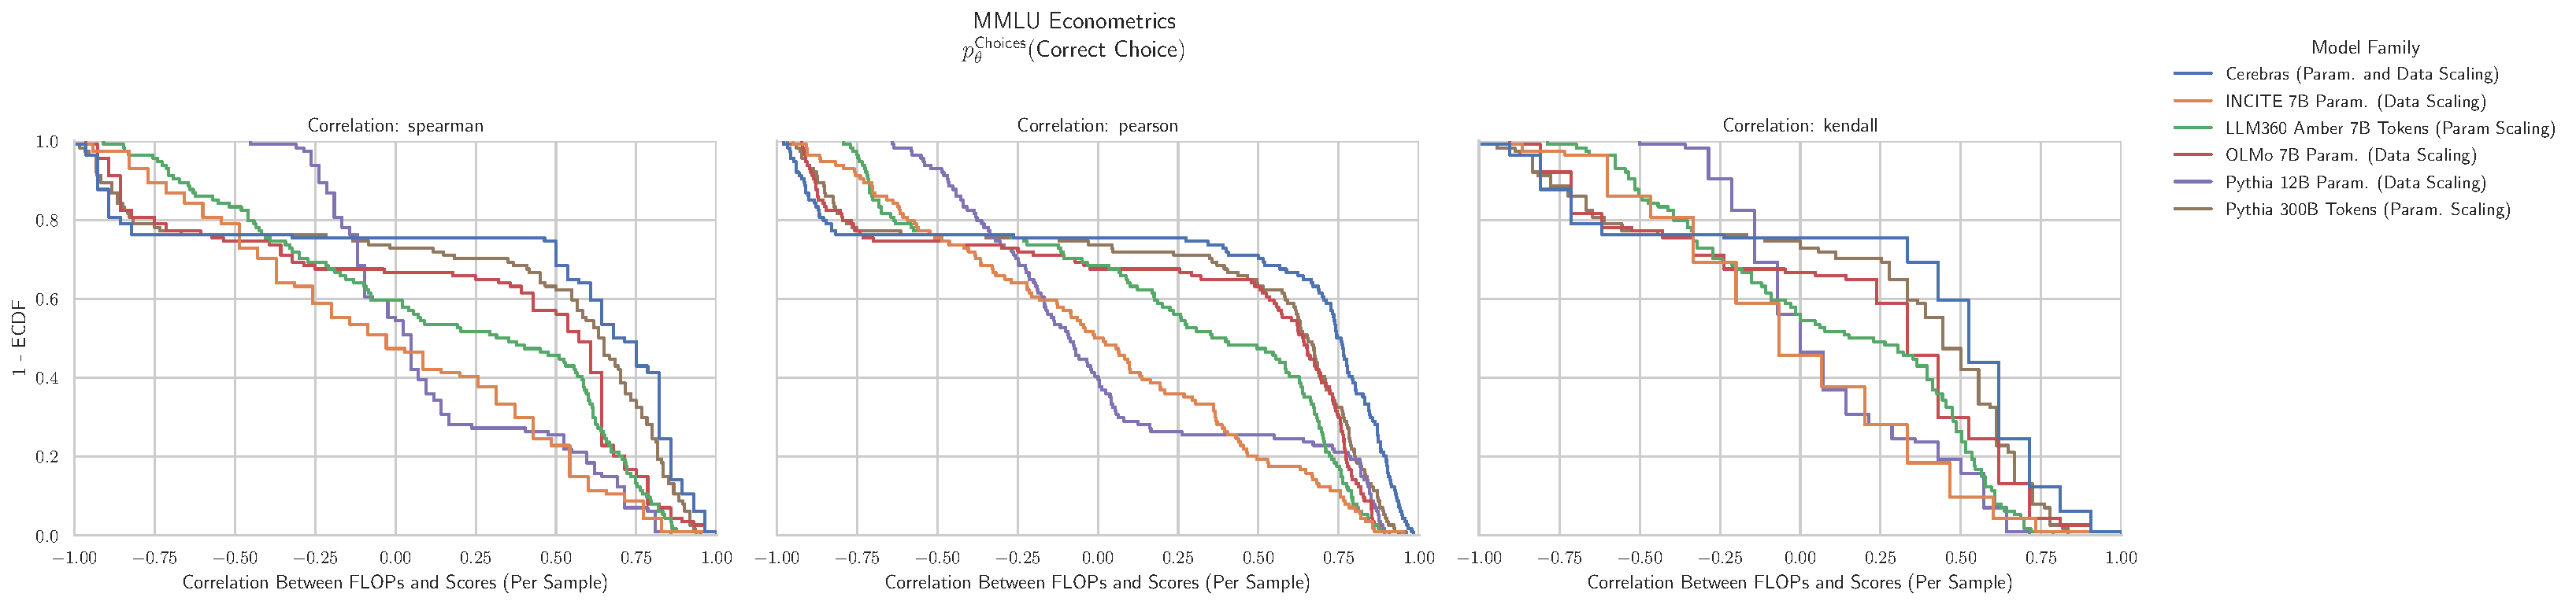
\includegraphics[width=\textwidth]{figures/correlations_between_scores_and_compute/correlation_distributions/mmlu_econometrics/mmlu_econometrics_prob_correct_choices_ecdf_vs_correlation_score_by_modelfamily_split_correlation_metric.pdf}
    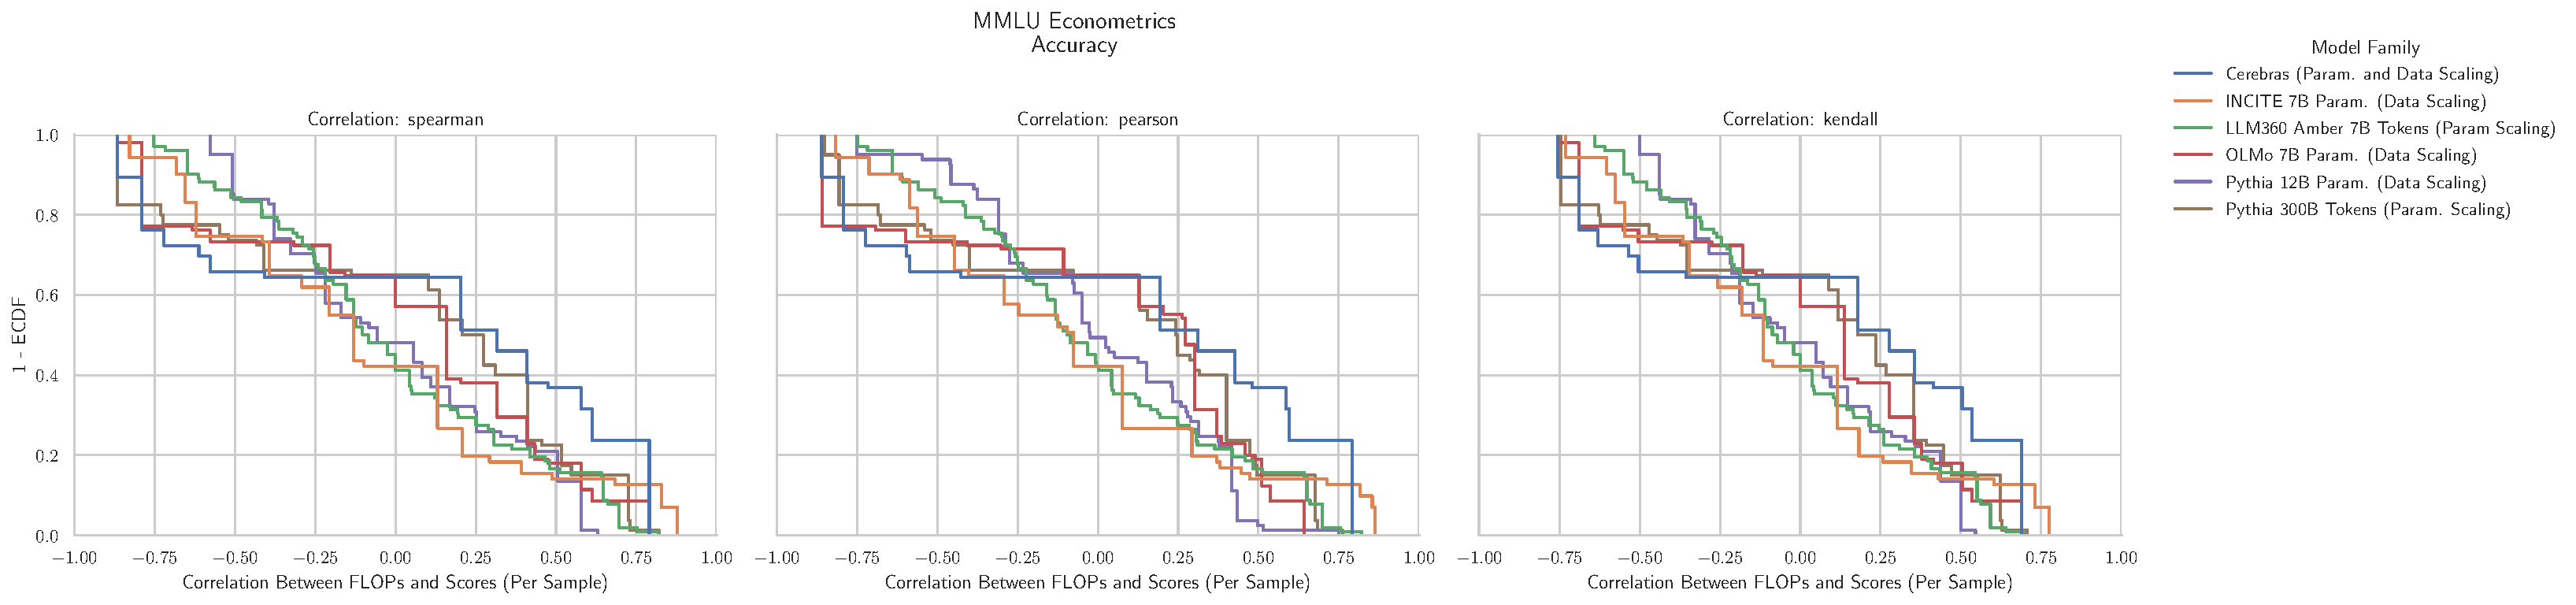
\includegraphics[width=\textwidth]{figures/correlations_between_scores_and_compute/correlation_distributions/mmlu_econometrics/mmlu_econometrics_acc_ecdf_vs_correlation_score_by_modelfamily_split_correlation_metric.pdf}
    \caption{\textbf{MMLU Econometrics: Downstream performance is computed via a sequence of transformations that deteriorate correlations between scores and pretraining compute.}}
    \label{app:fig:compute_score_distribution_mmlu_econometrics}
\end{figure}

\clearpage
\subsection{NLP Benchmark: MMLU Electrical Engineering \cite{hendrycks2020mmlu}}

\begin{figure}[h!]
    \centering
    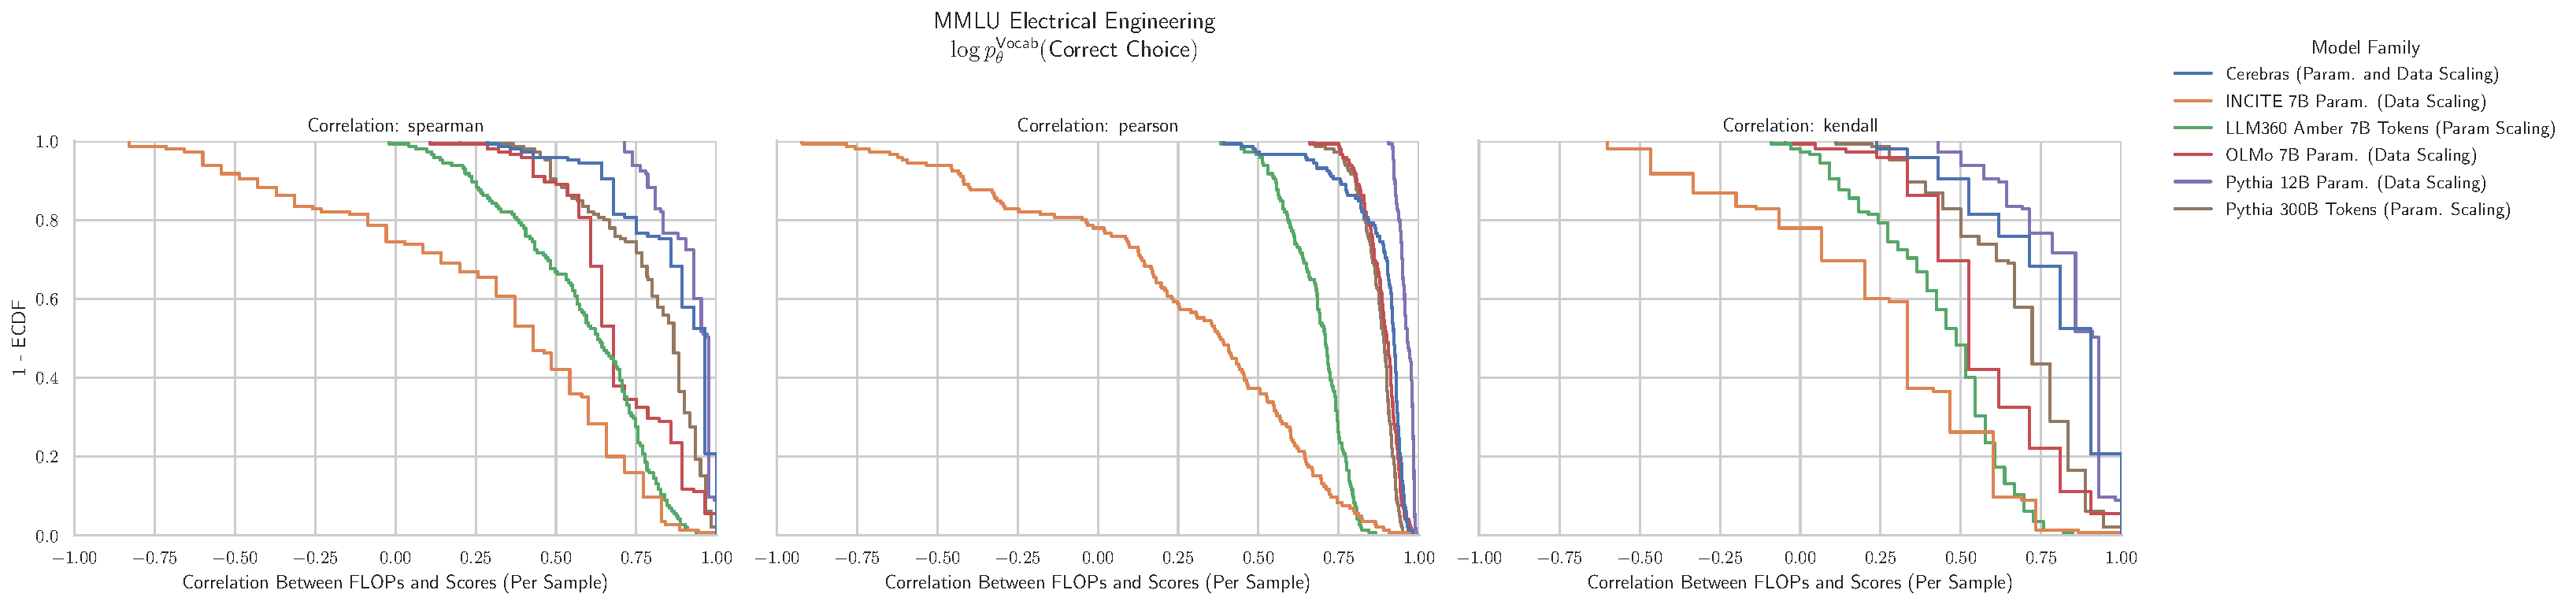
\includegraphics[width=\textwidth]{figures/correlations_between_scores_and_compute/correlation_distributions/mmlu_electrical_engineering/mmlu_electrical_engineering_log_likelihood_correct_ecdf_vs_correlation_score_by_modelfamily_split_correlation_metric.pdf}
    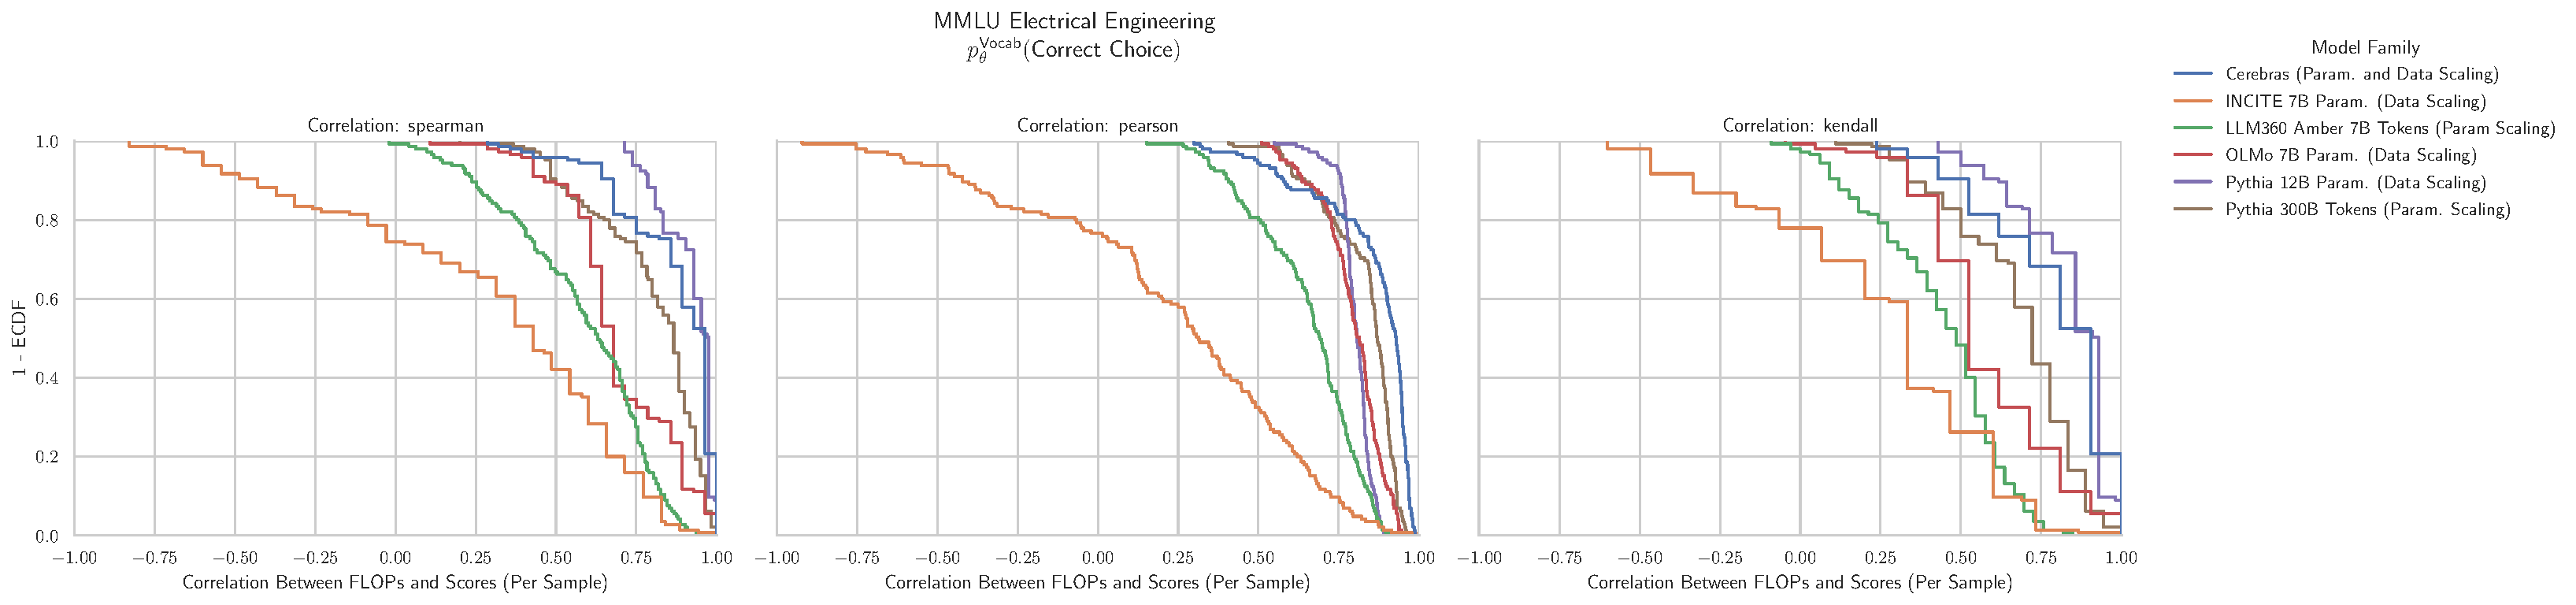
\includegraphics[width=\textwidth]{figures/correlations_between_scores_and_compute/correlation_distributions/mmlu_electrical_engineering/mmlu_electrical_engineering_prob_correct_vocab_ecdf_vs_correlation_score_by_modelfamily_split_correlation_metric.pdf}
    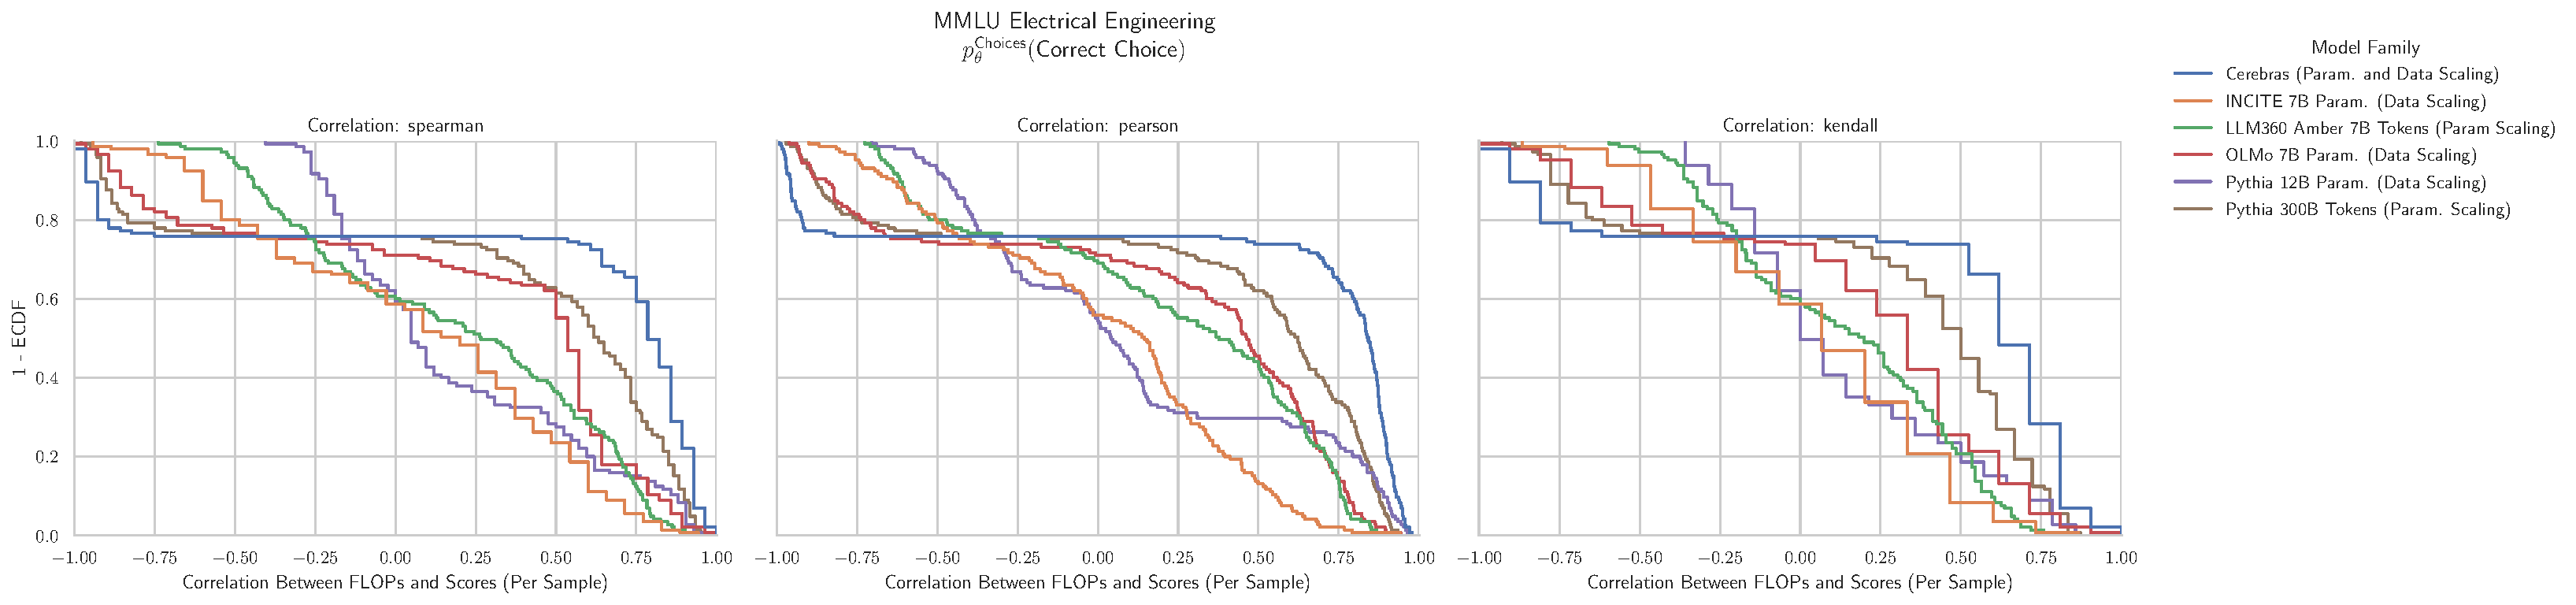
\includegraphics[width=\textwidth]{figures/correlations_between_scores_and_compute/correlation_distributions/mmlu_electrical_engineering/mmlu_electrical_engineering_prob_correct_choices_ecdf_vs_correlation_score_by_modelfamily_split_correlation_metric.pdf}
    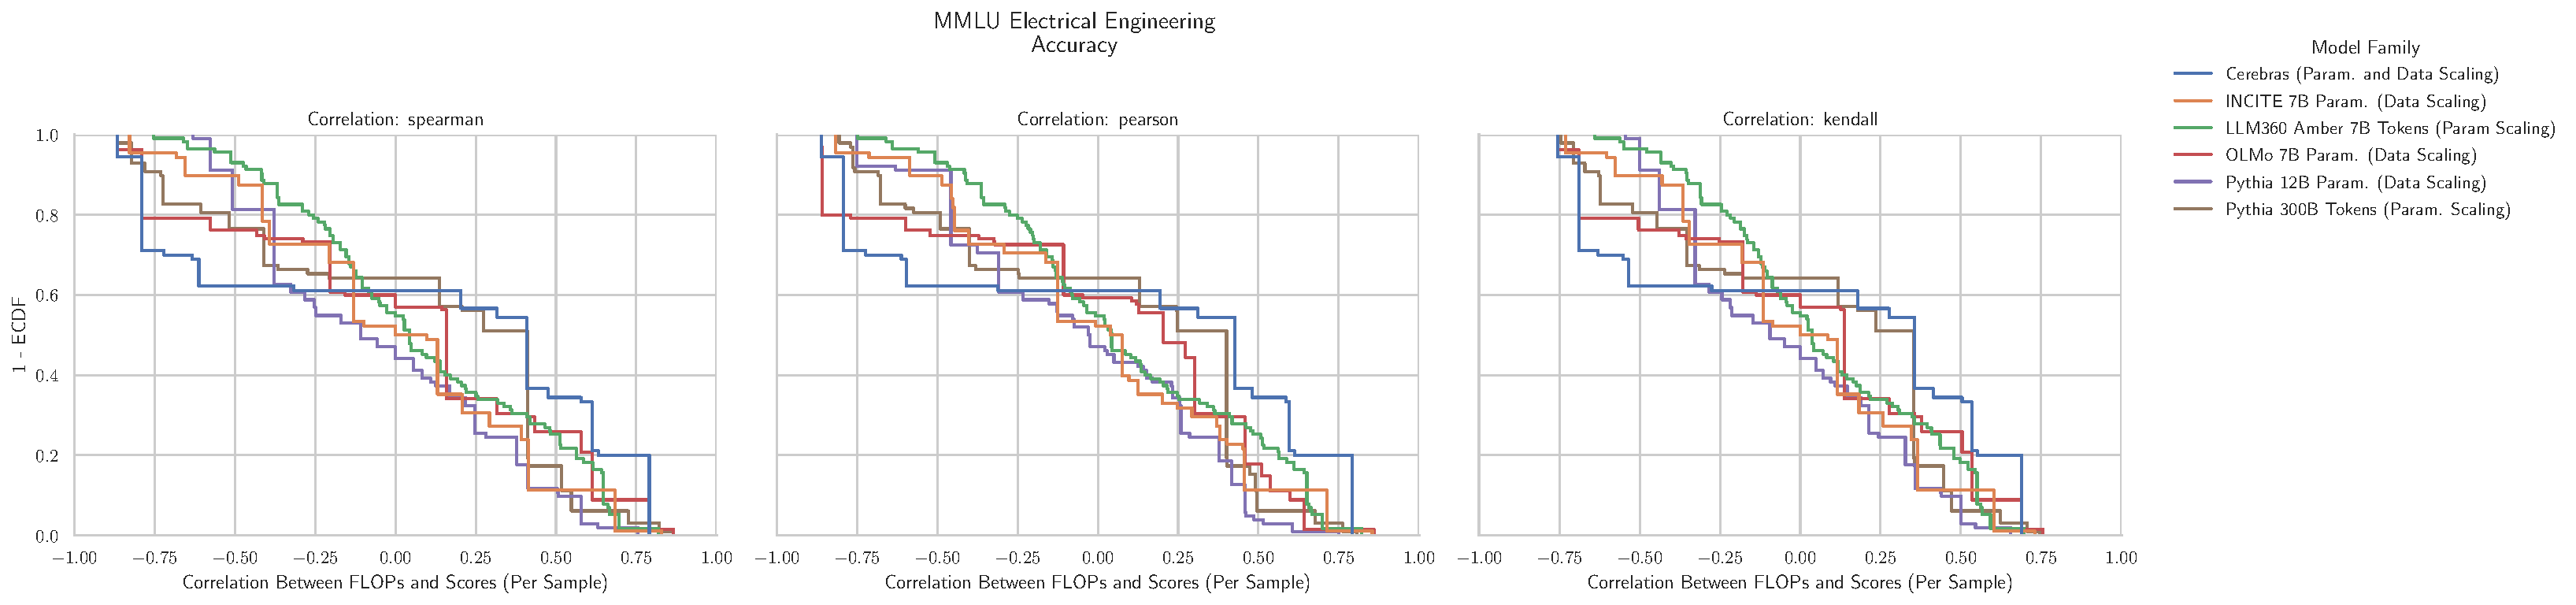
\includegraphics[width=\textwidth]{figures/correlations_between_scores_and_compute/correlation_distributions/mmlu_electrical_engineering/mmlu_electrical_engineering_acc_ecdf_vs_correlation_score_by_modelfamily_split_correlation_metric.pdf}
    \caption{\textbf{MMLU Electrical Engineering: Downstream performance is computed via a sequence of transformations that deteriorate correlations between scores and pretraining compute.}}
    \label{app:fig:compute_score_distribution_mmlu_electrical_engineering}
\end{figure}

\clearpage
\subsection{NLP Benchmark: MMLU Elementary Mathematics \cite{hendrycks2020mmlu}}

\begin{figure}[h!]
    \centering
    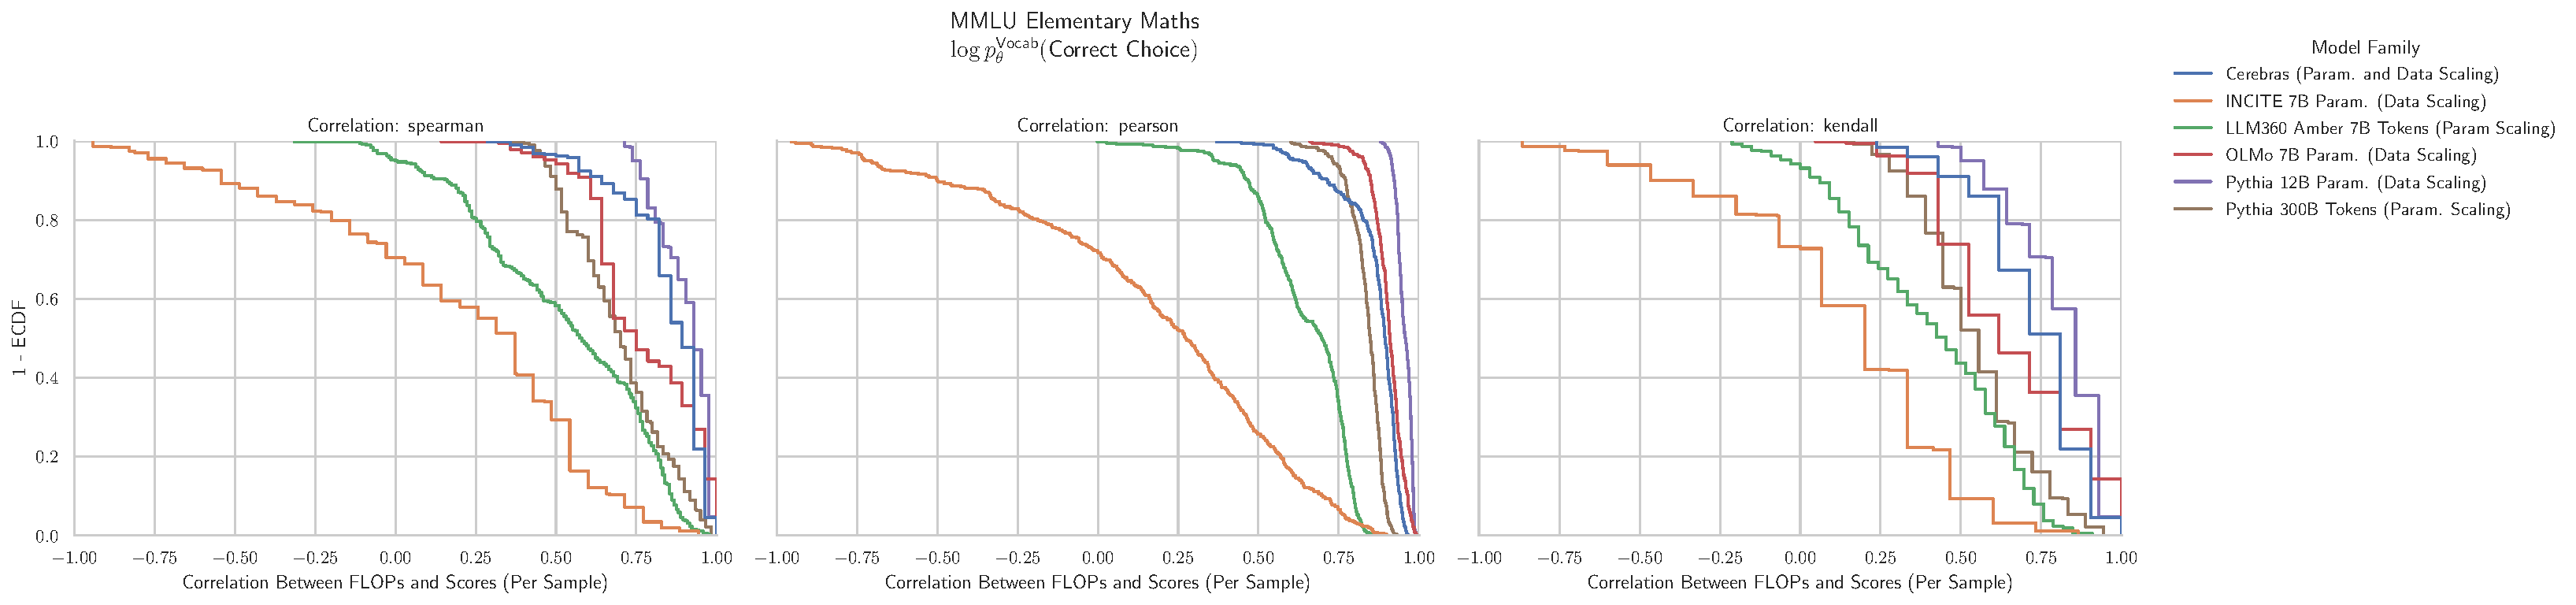
\includegraphics[width=\textwidth]{figures/correlations_between_scores_and_compute/correlation_distributions/mmlu_elementary_mathematics/mmlu_elementary_mathematics_log_likelihood_correct_ecdf_vs_correlation_score_by_modelfamily_split_correlation_metric.pdf}
    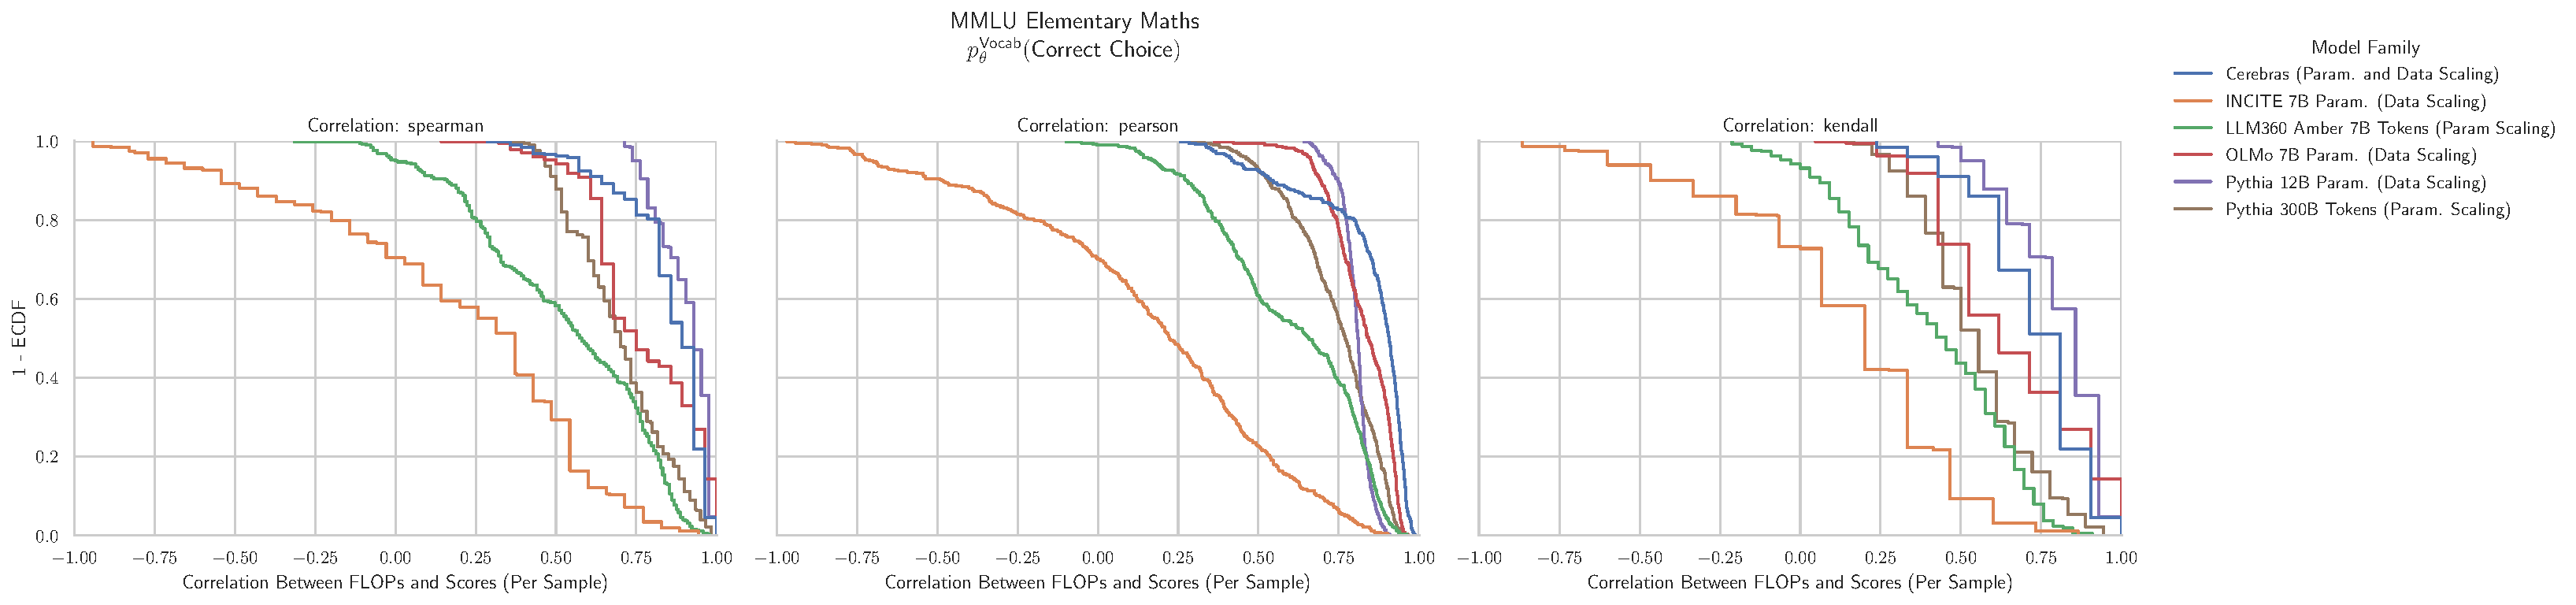
\includegraphics[width=\textwidth]{figures/correlations_between_scores_and_compute/correlation_distributions/mmlu_elementary_mathematics/mmlu_elementary_mathematics_prob_correct_vocab_ecdf_vs_correlation_score_by_modelfamily_split_correlation_metric.pdf}
    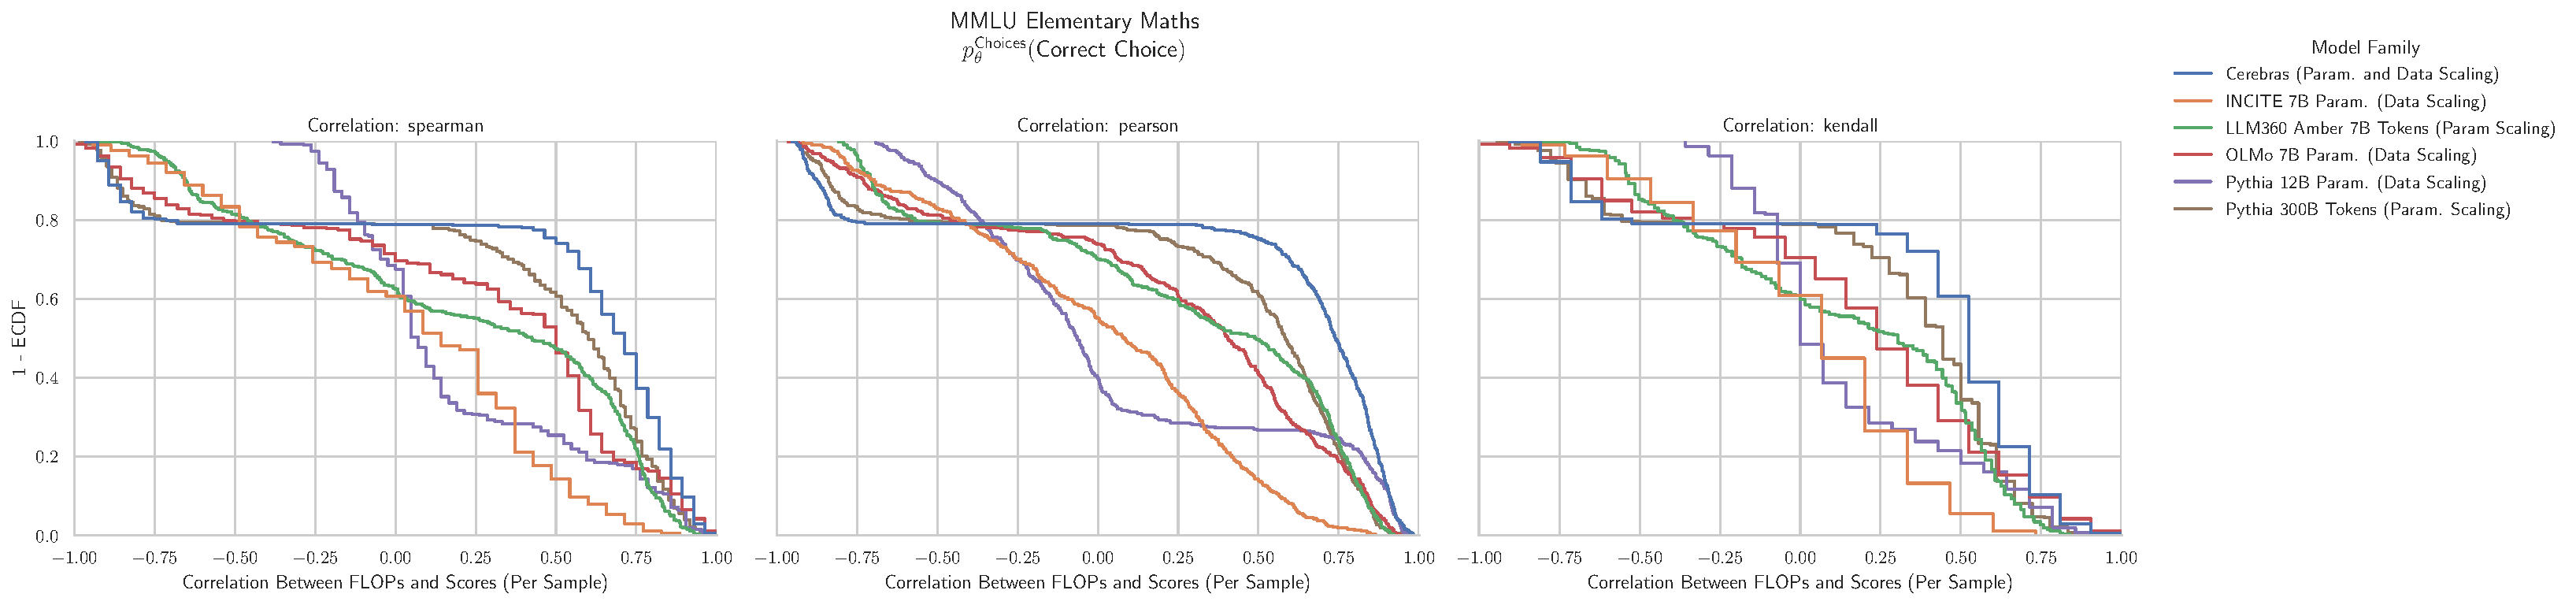
\includegraphics[width=\textwidth]{figures/correlations_between_scores_and_compute/correlation_distributions/mmlu_elementary_mathematics/mmlu_elementary_mathematics_prob_correct_choices_ecdf_vs_correlation_score_by_modelfamily_split_correlation_metric.pdf}
    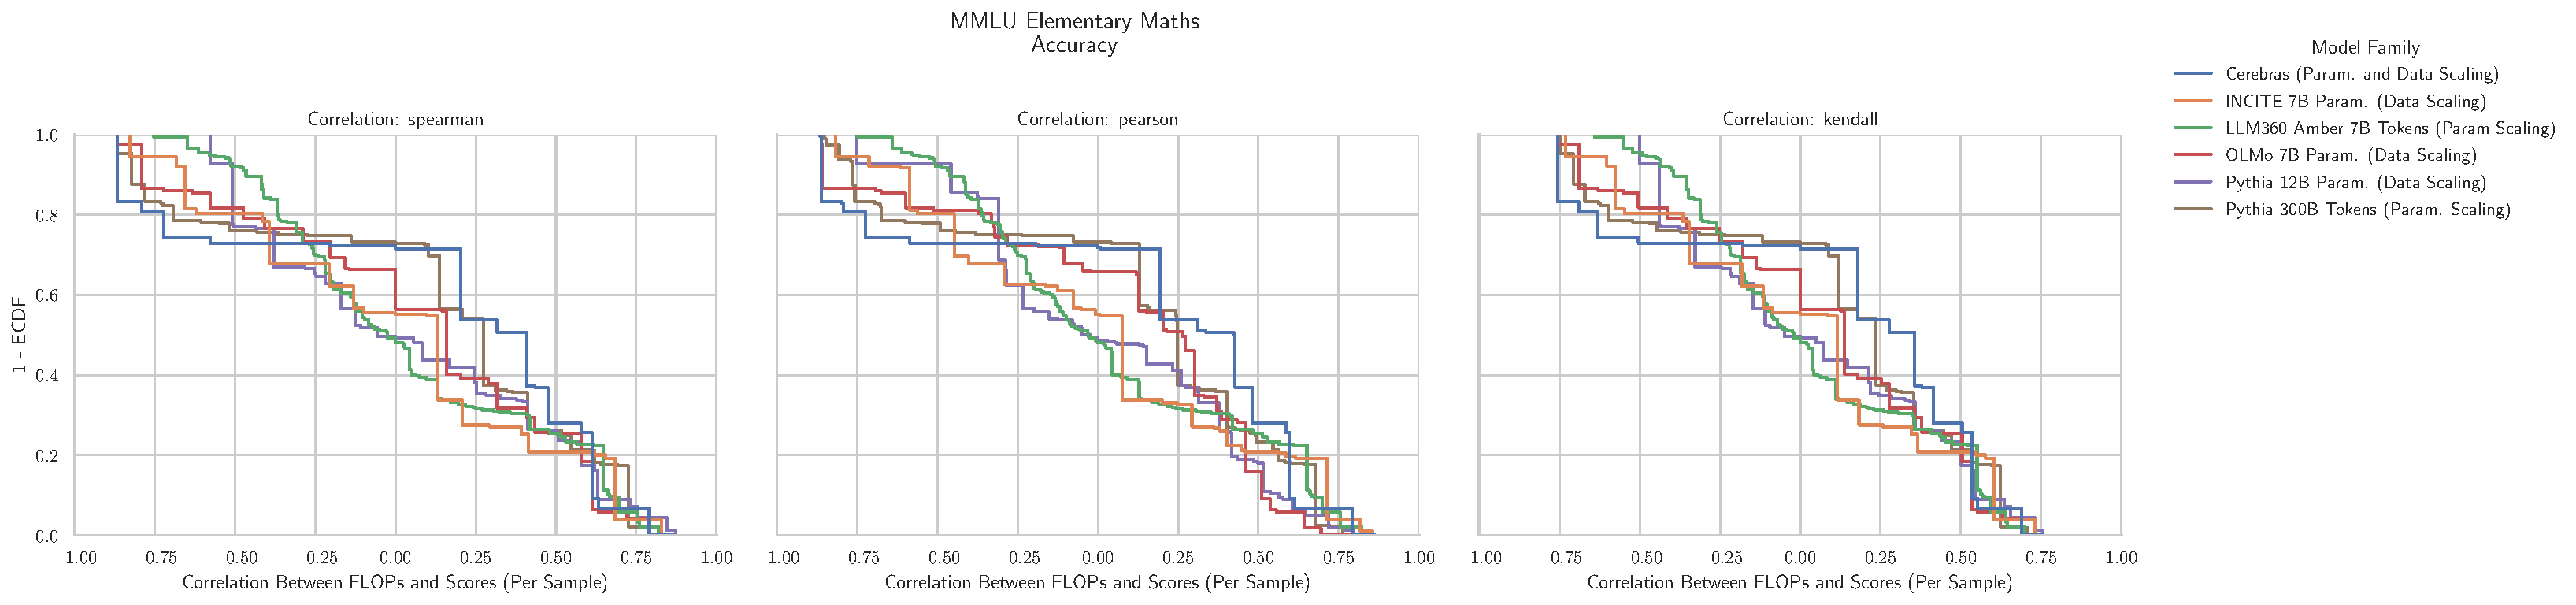
\includegraphics[width=\textwidth]{figures/correlations_between_scores_and_compute/correlation_distributions/mmlu_elementary_mathematics/mmlu_elementary_mathematics_acc_ecdf_vs_correlation_score_by_modelfamily_split_correlation_metric.pdf}
    \caption{\textbf{MMLU Elementary Mathematics: Downstream performance is computed via a sequence of transformations that deteriorate correlations between scores and pretraining compute.}}
    \label{app:fig:compute_score_distribution_mmlu_elementary_mathematics}
\end{figure}

\clearpage
\subsection{NLP Benchmark: MMLU Formal Logic \cite{hendrycks2020mmlu}}

\begin{figure}[h!]
    \centering
    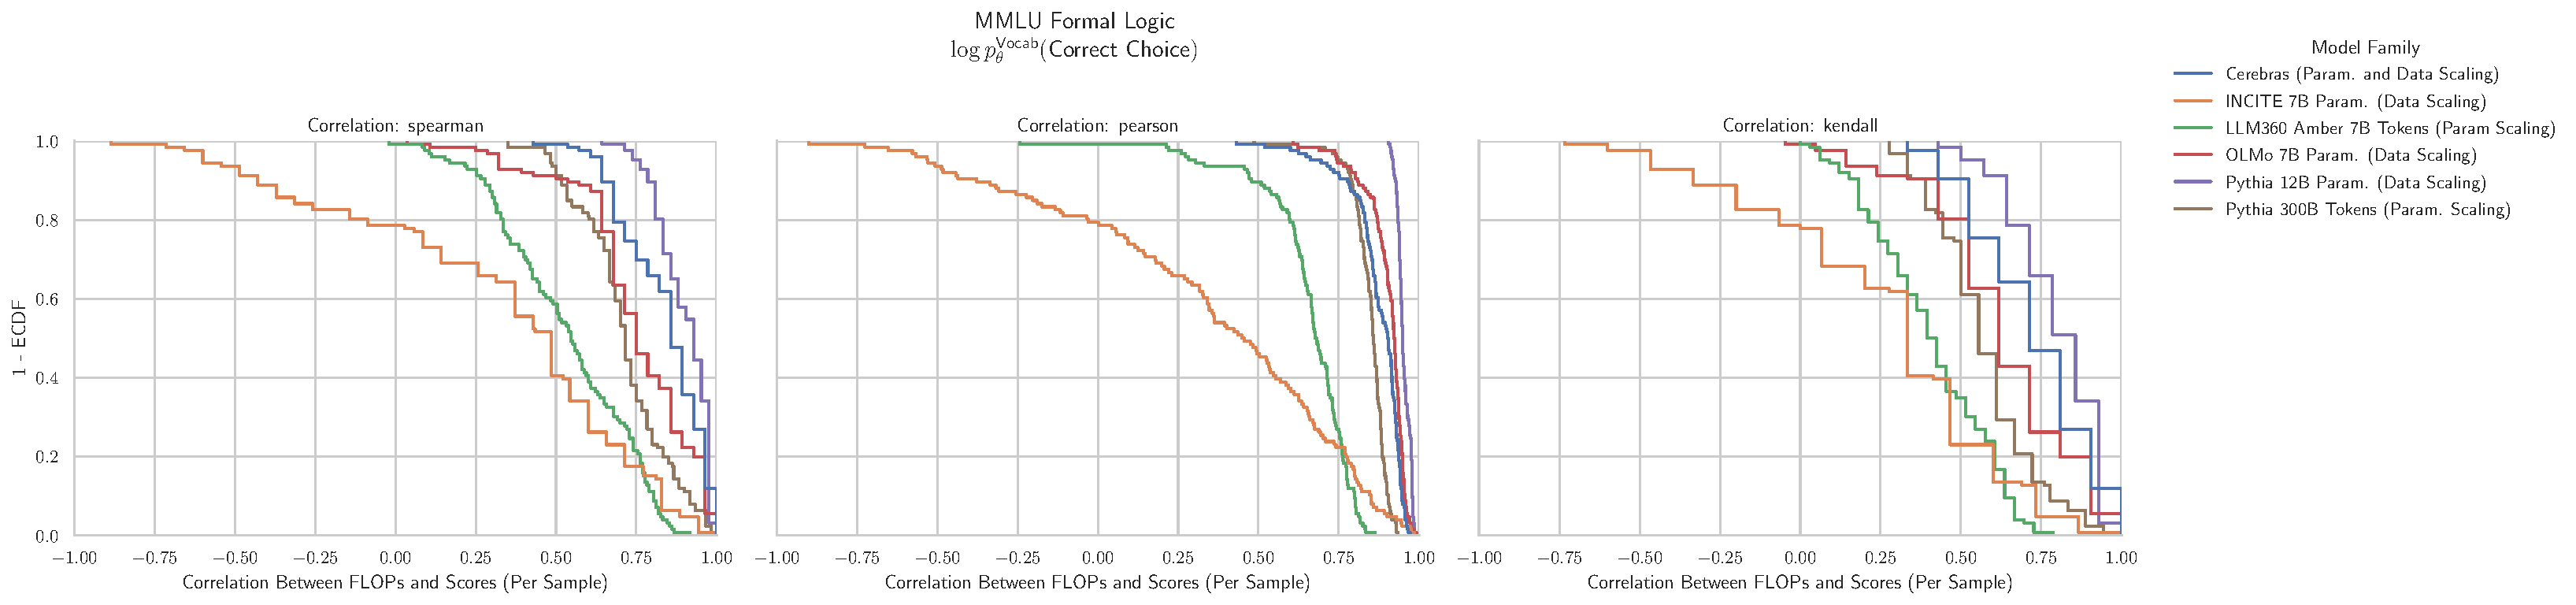
\includegraphics[width=\textwidth]{figures/correlations_between_scores_and_compute/correlation_distributions/mmlu_formal_logic/mmlu_formal_logic_log_likelihood_correct_ecdf_vs_correlation_score_by_modelfamily_split_correlation_metric.pdf}
    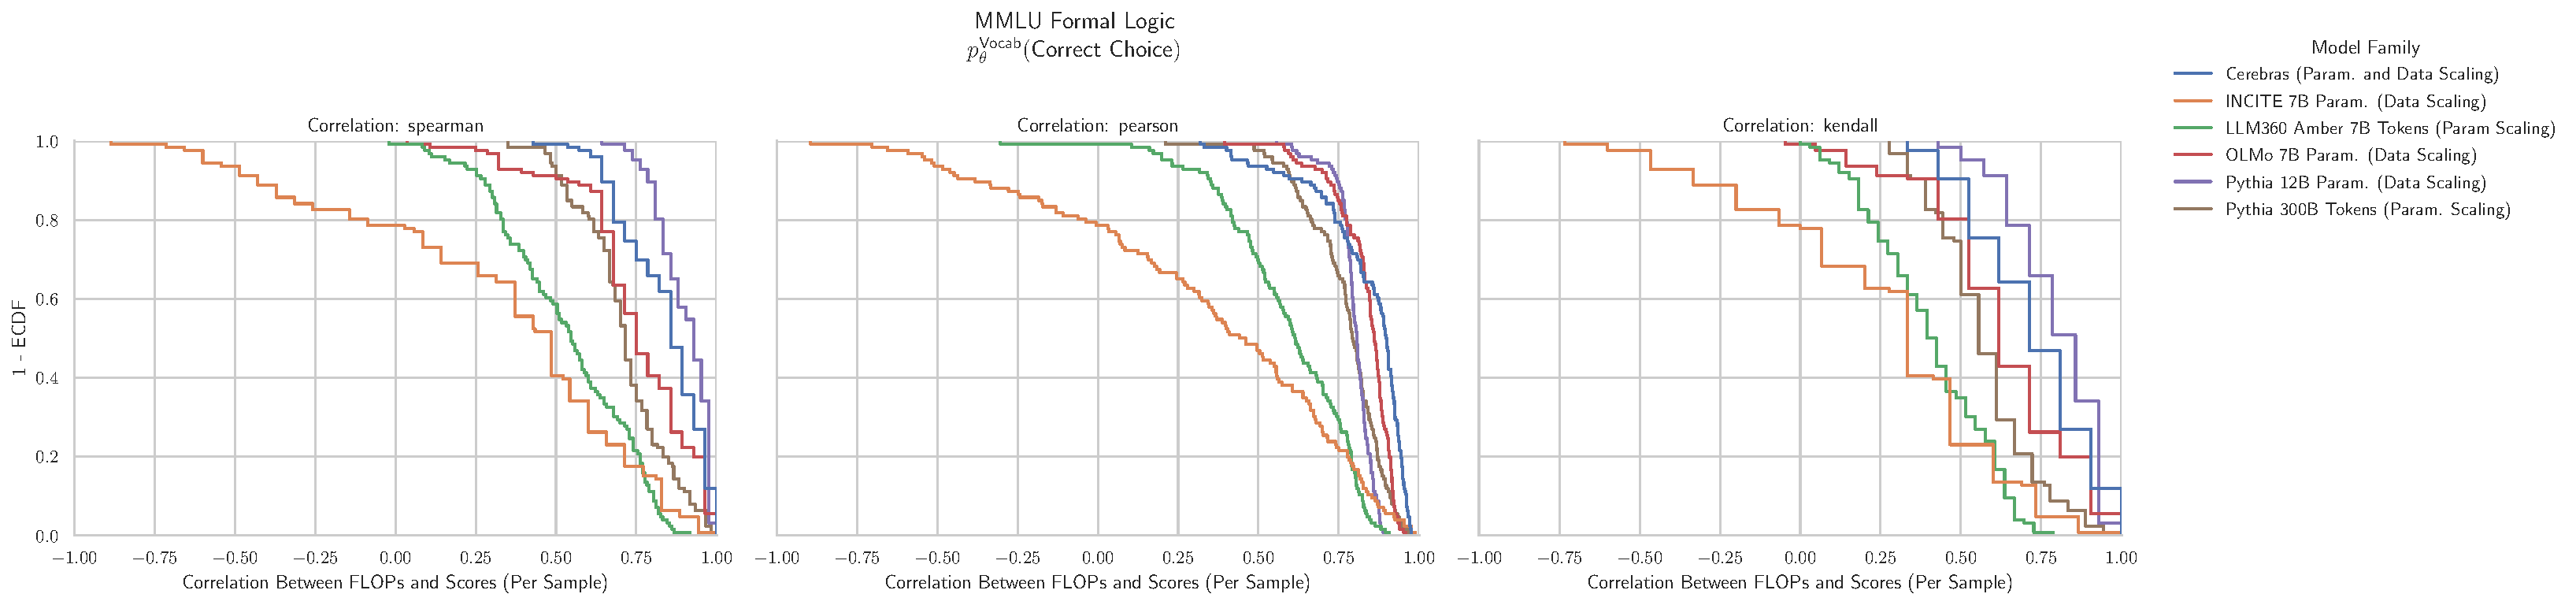
\includegraphics[width=\textwidth]{figures/correlations_between_scores_and_compute/correlation_distributions/mmlu_formal_logic/mmlu_formal_logic_prob_correct_vocab_ecdf_vs_correlation_score_by_modelfamily_split_correlation_metric.pdf}
    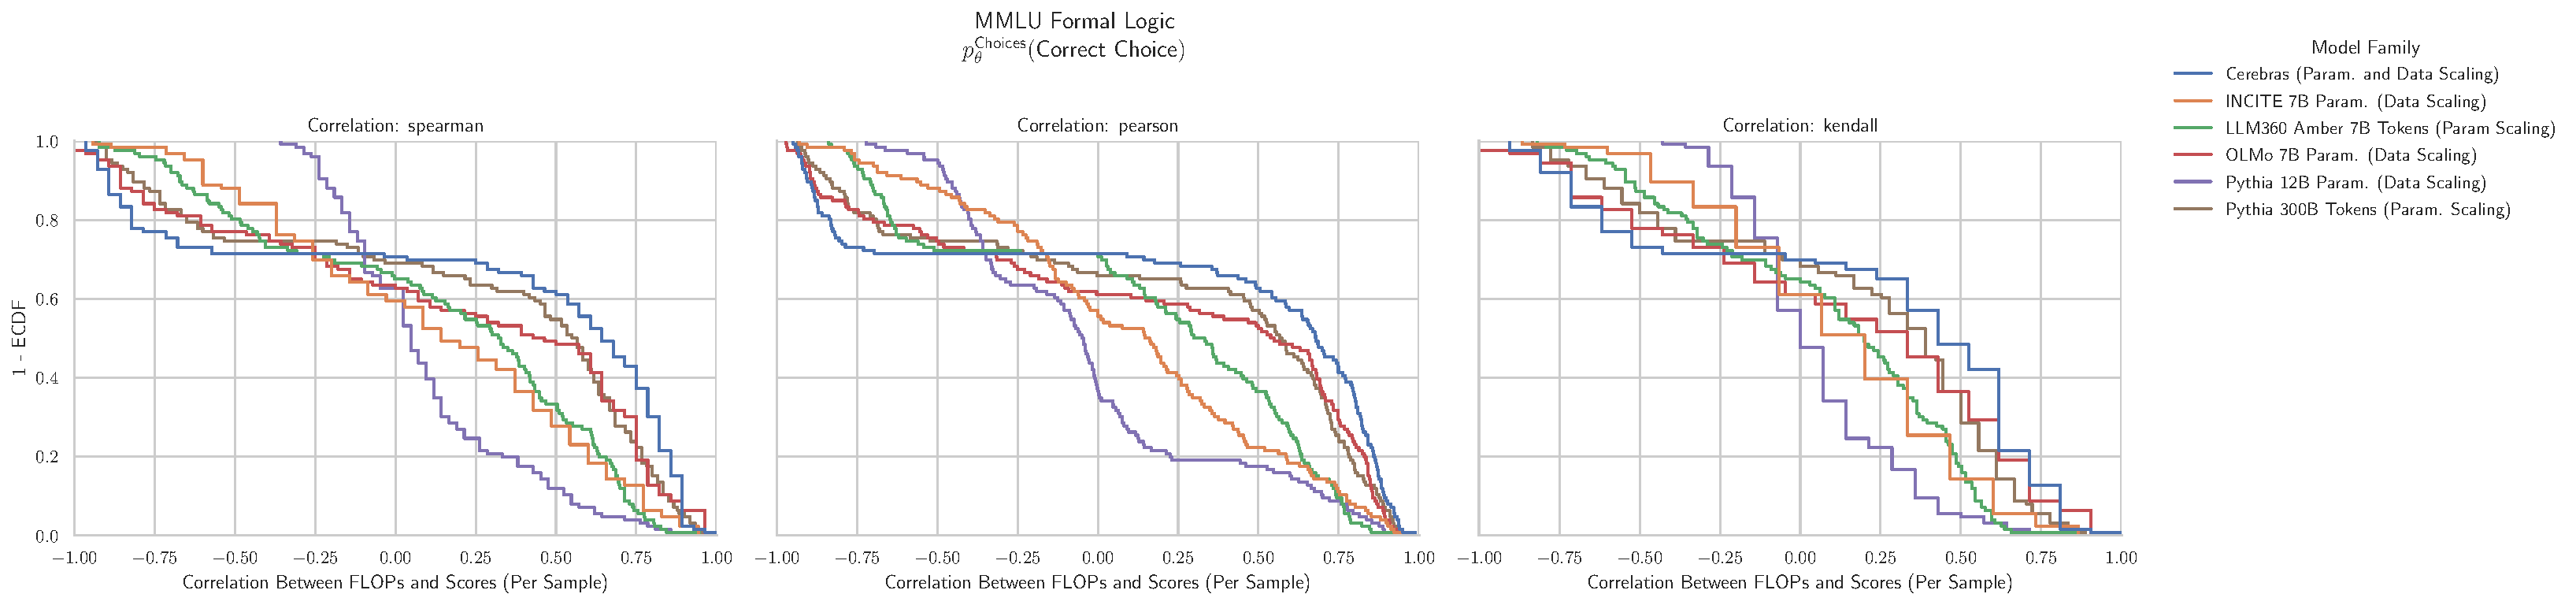
\includegraphics[width=\textwidth]{figures/correlations_between_scores_and_compute/correlation_distributions/mmlu_formal_logic/mmlu_formal_logic_prob_correct_choices_ecdf_vs_correlation_score_by_modelfamily_split_correlation_metric.pdf}
    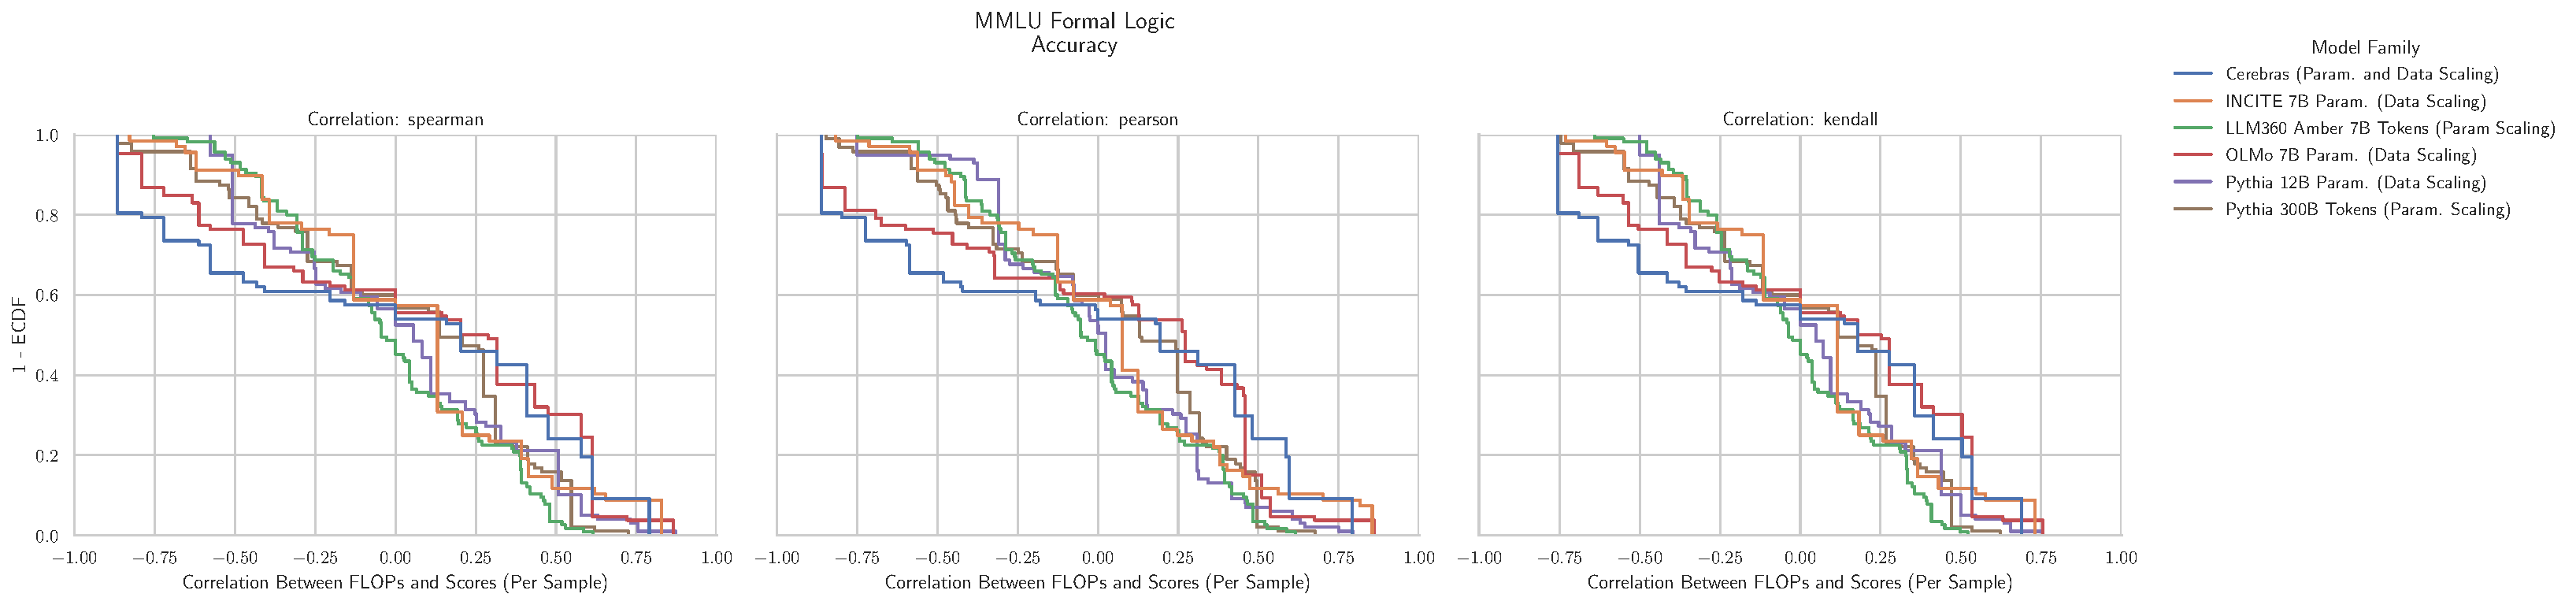
\includegraphics[width=\textwidth]{figures/correlations_between_scores_and_compute/correlation_distributions/mmlu_formal_logic/mmlu_formal_logic_acc_ecdf_vs_correlation_score_by_modelfamily_split_correlation_metric.pdf}
    \caption{\textbf{MMLU Formal Logic: Downstream performance is computed via a sequence of transformations that deteriorate correlations between scores and pretraining compute.}}
    \label{app:fig:compute_score_distribution_mmlu_formal_logic}
\end{figure}

\clearpage
\subsection{NLP Benchmark: MMLU Global Facts \cite{hendrycks2020mmlu}}

\begin{figure}[h!]
    \centering
    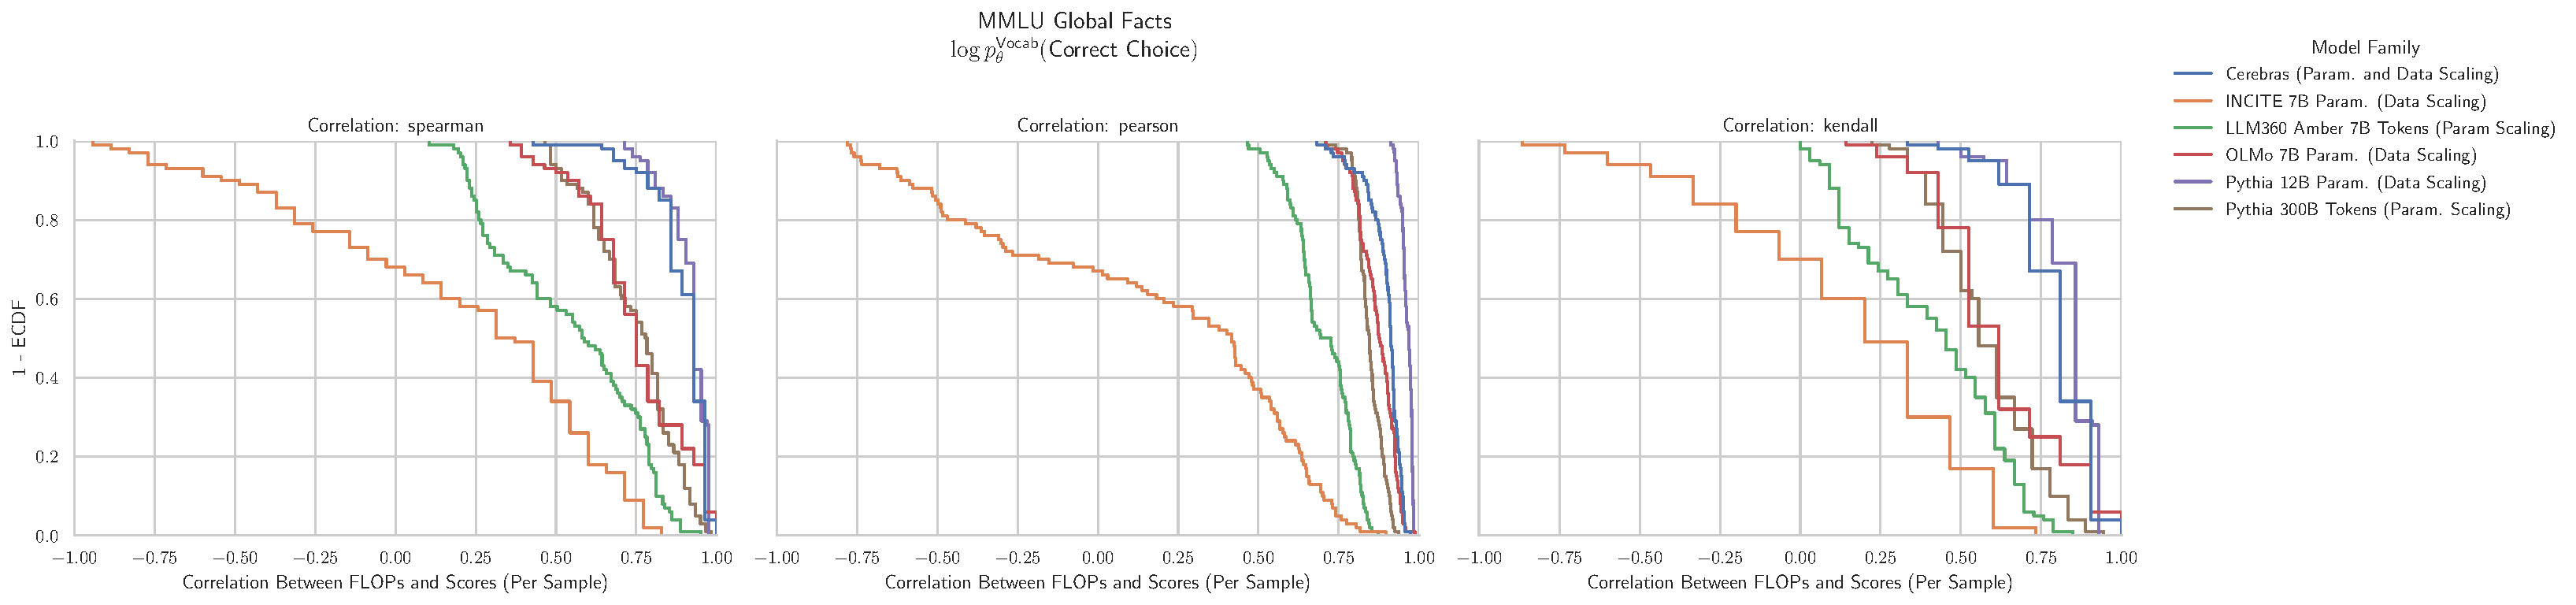
\includegraphics[width=\textwidth]{figures/correlations_between_scores_and_compute/correlation_distributions/mmlu_global_facts/mmlu_global_facts_log_likelihood_correct_ecdf_vs_correlation_score_by_modelfamily_split_correlation_metric.pdf}
    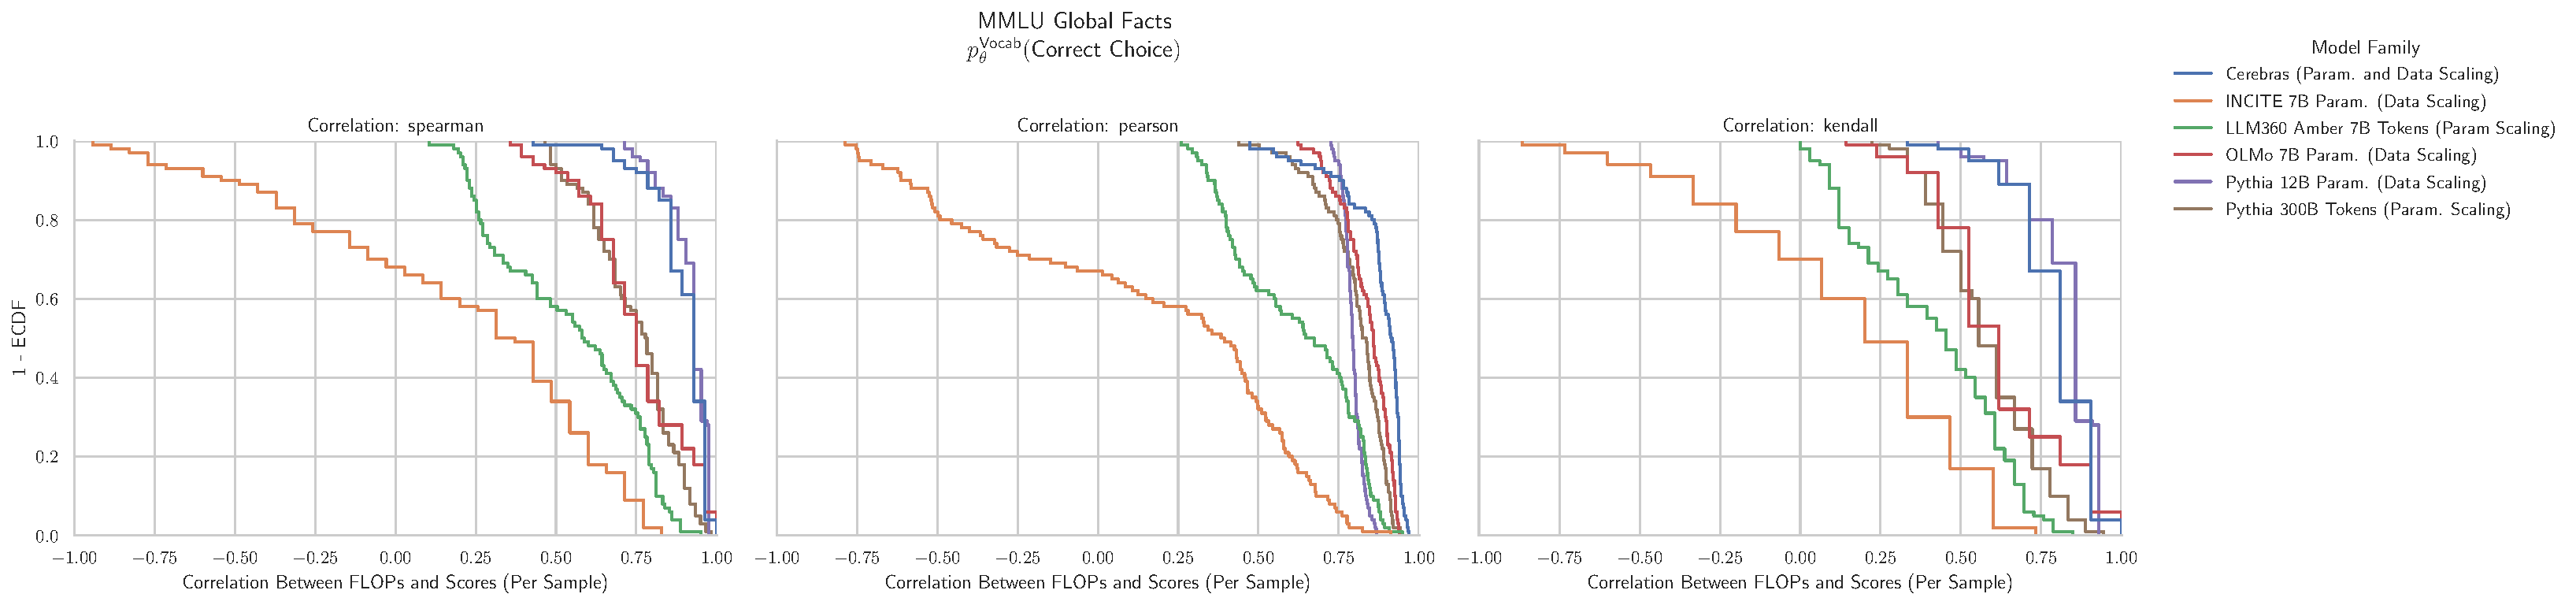
\includegraphics[width=\textwidth]{figures/correlations_between_scores_and_compute/correlation_distributions/mmlu_global_facts/mmlu_global_facts_prob_correct_vocab_ecdf_vs_correlation_score_by_modelfamily_split_correlation_metric.pdf}
    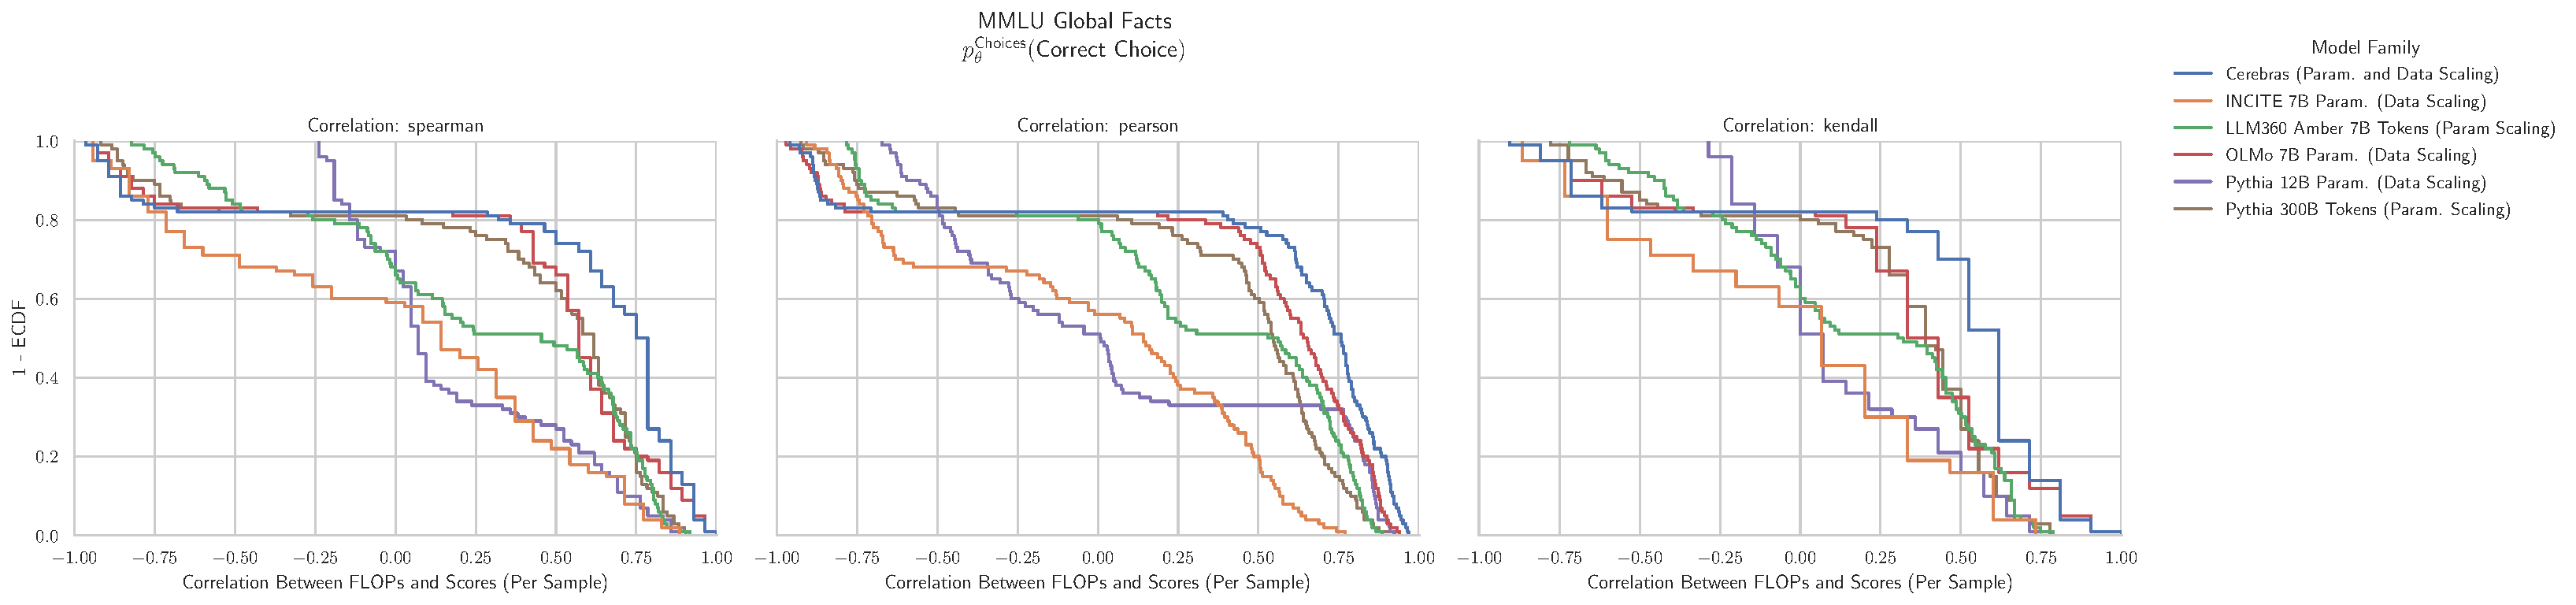
\includegraphics[width=\textwidth]{figures/correlations_between_scores_and_compute/correlation_distributions/mmlu_global_facts/mmlu_global_facts_prob_correct_choices_ecdf_vs_correlation_score_by_modelfamily_split_correlation_metric.pdf}
    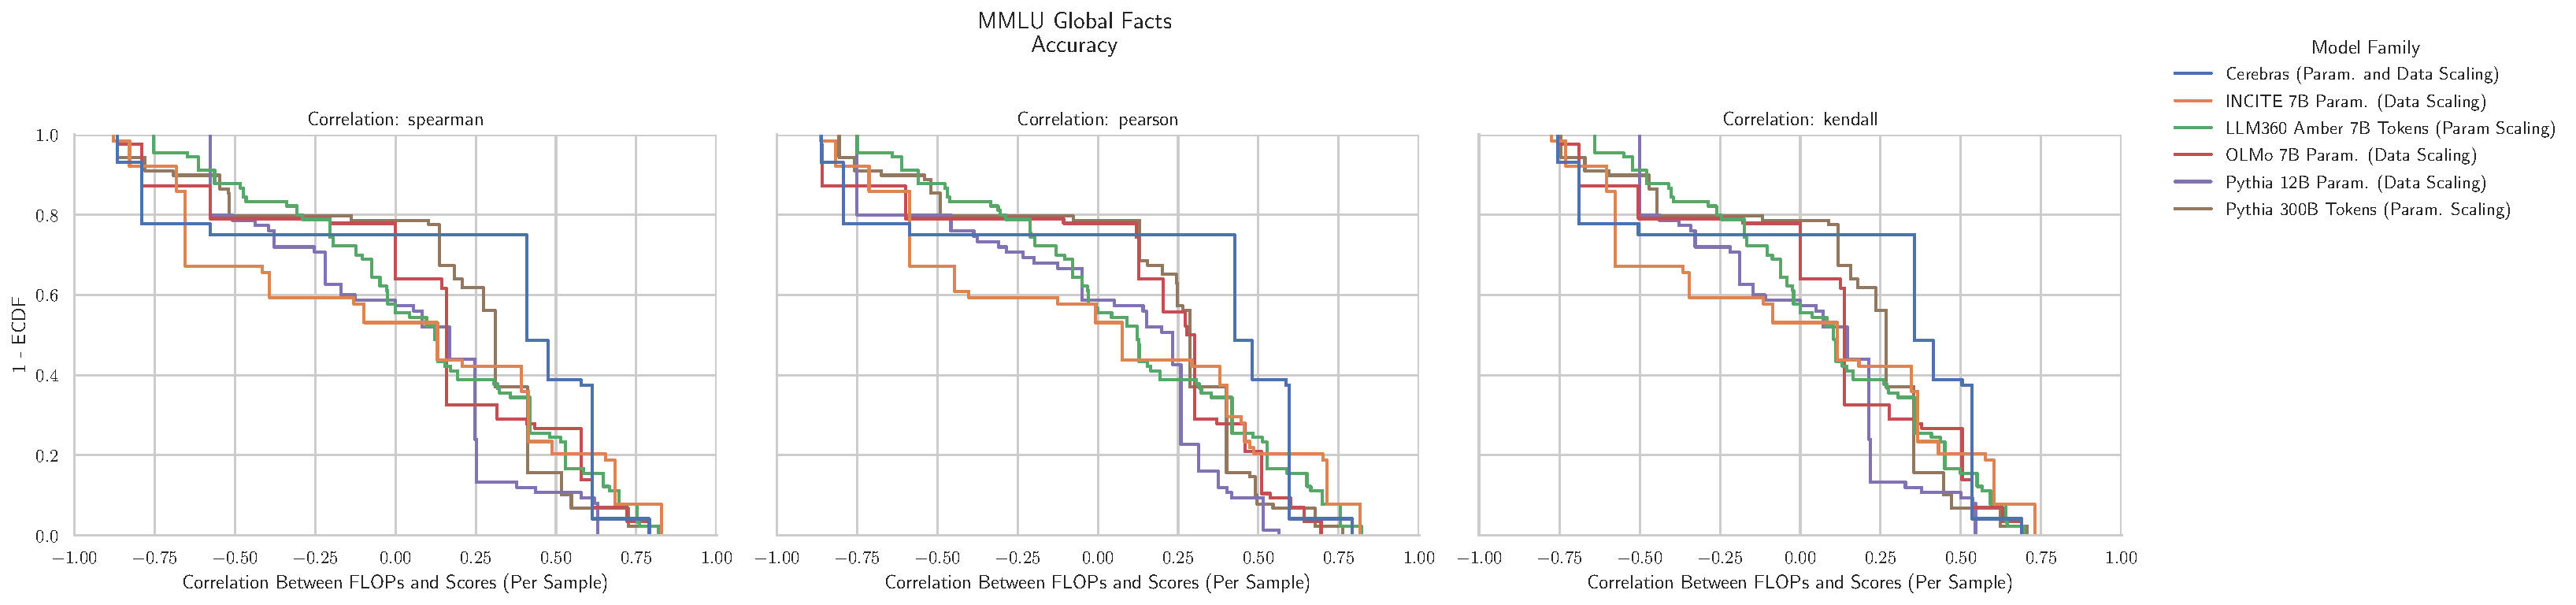
\includegraphics[width=\textwidth]{figures/correlations_between_scores_and_compute/correlation_distributions/mmlu_global_facts/mmlu_global_facts_acc_ecdf_vs_correlation_score_by_modelfamily_split_correlation_metric.pdf}
    \caption{\textbf{MMLU Global Facts: Downstream performance is computed via a sequence of transformations that deteriorate correlations between scores and pretraining compute.}}
    \label{app:fig:compute_score_distribution_mmlu_global_facts}
\end{figure}


\clearpage
\subsection{NLP Benchmark: MMLU High School Biology \cite{hendrycks2020mmlu}}

\begin{figure}[h!]
    \centering
    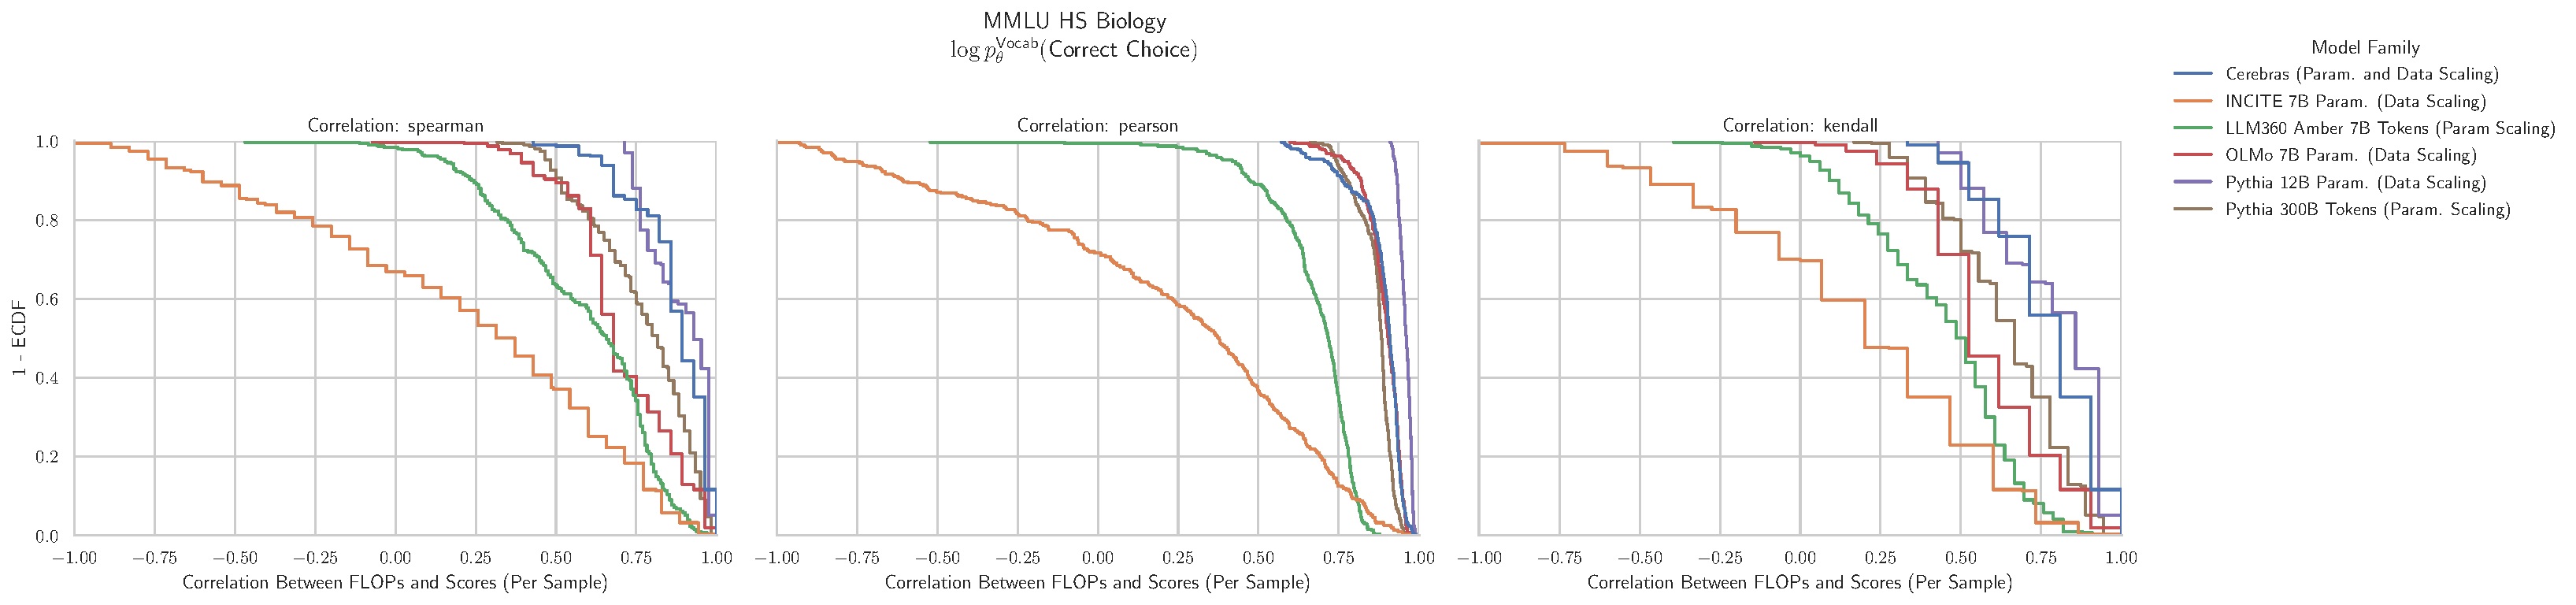
\includegraphics[width=\textwidth]{figures/correlations_between_scores_and_compute/correlation_distributions/mmlu_high_school_biology/mmlu_high_school_biology_log_likelihood_correct_ecdf_vs_correlation_score_by_modelfamily_split_correlation_metric.pdf}
    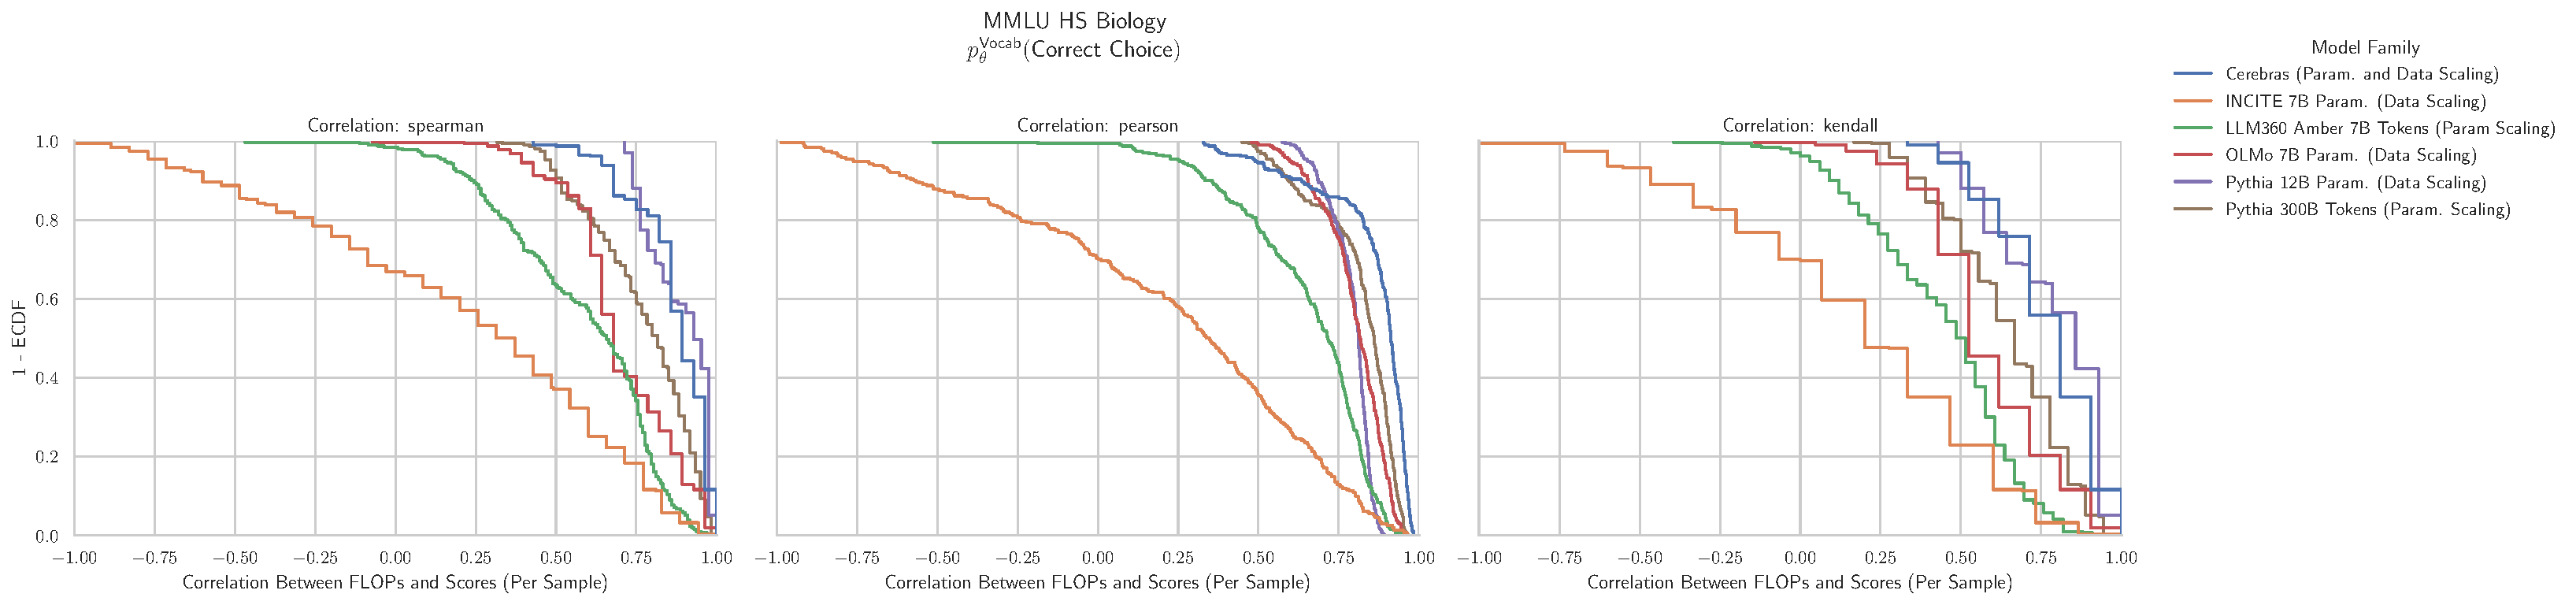
\includegraphics[width=\textwidth]{figures/correlations_between_scores_and_compute/correlation_distributions/mmlu_high_school_biology/mmlu_high_school_biology_prob_correct_vocab_ecdf_vs_correlation_score_by_modelfamily_split_correlation_metric.pdf}
    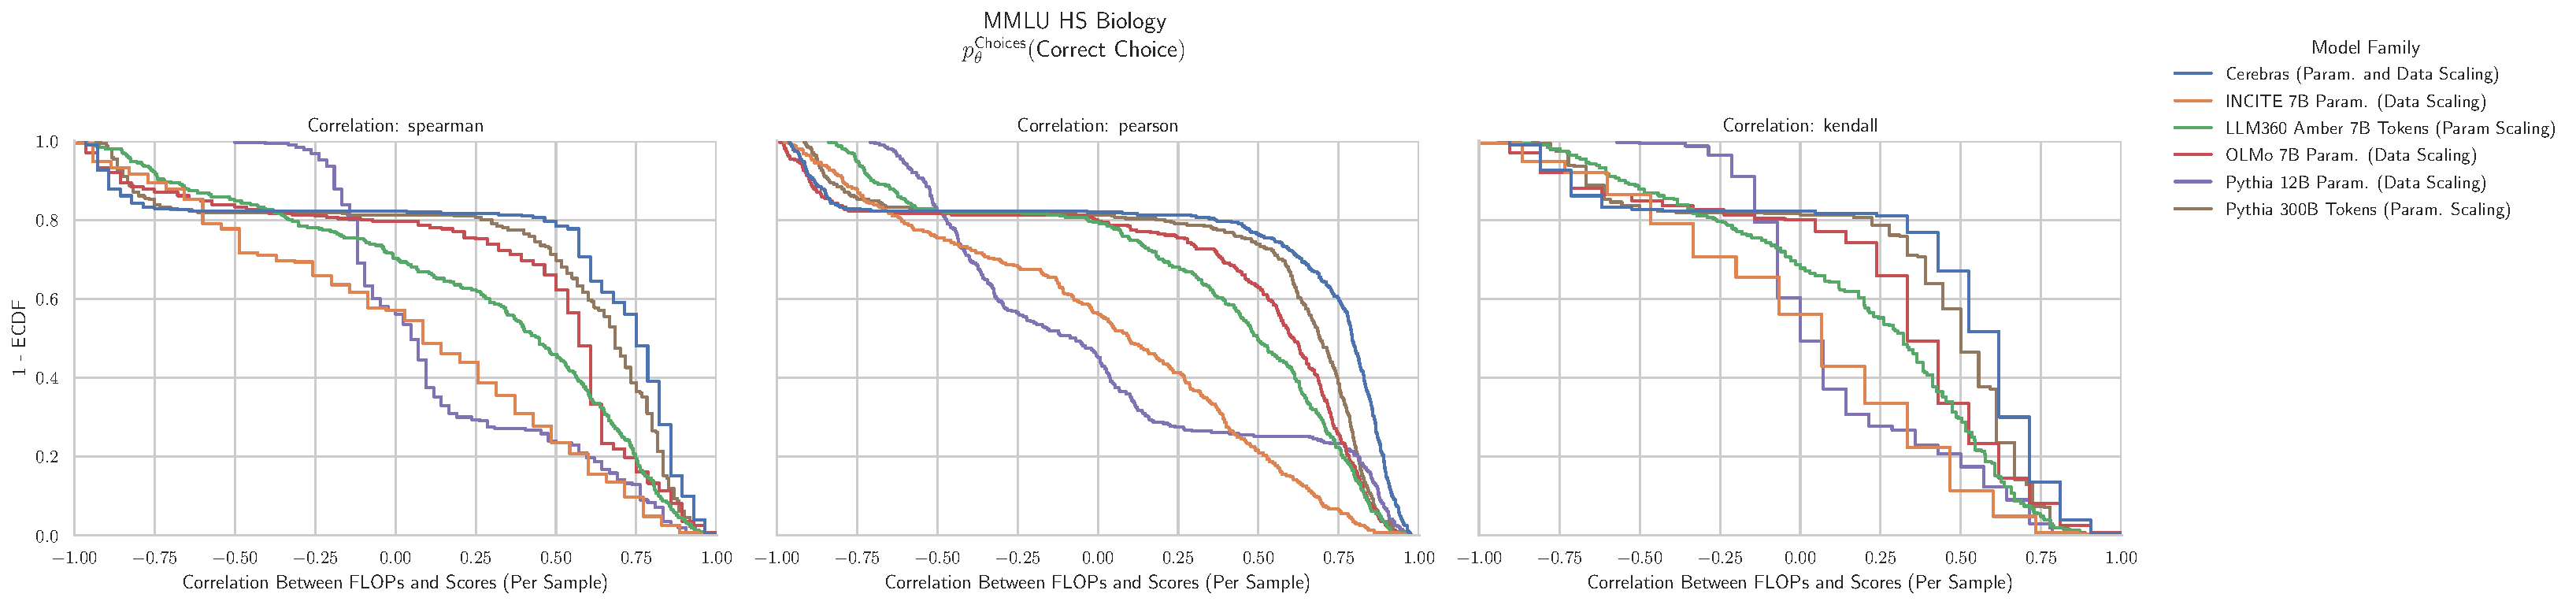
\includegraphics[width=\textwidth]{figures/correlations_between_scores_and_compute/correlation_distributions/mmlu_high_school_biology/mmlu_high_school_biology_prob_correct_choices_ecdf_vs_correlation_score_by_modelfamily_split_correlation_metric.pdf}
    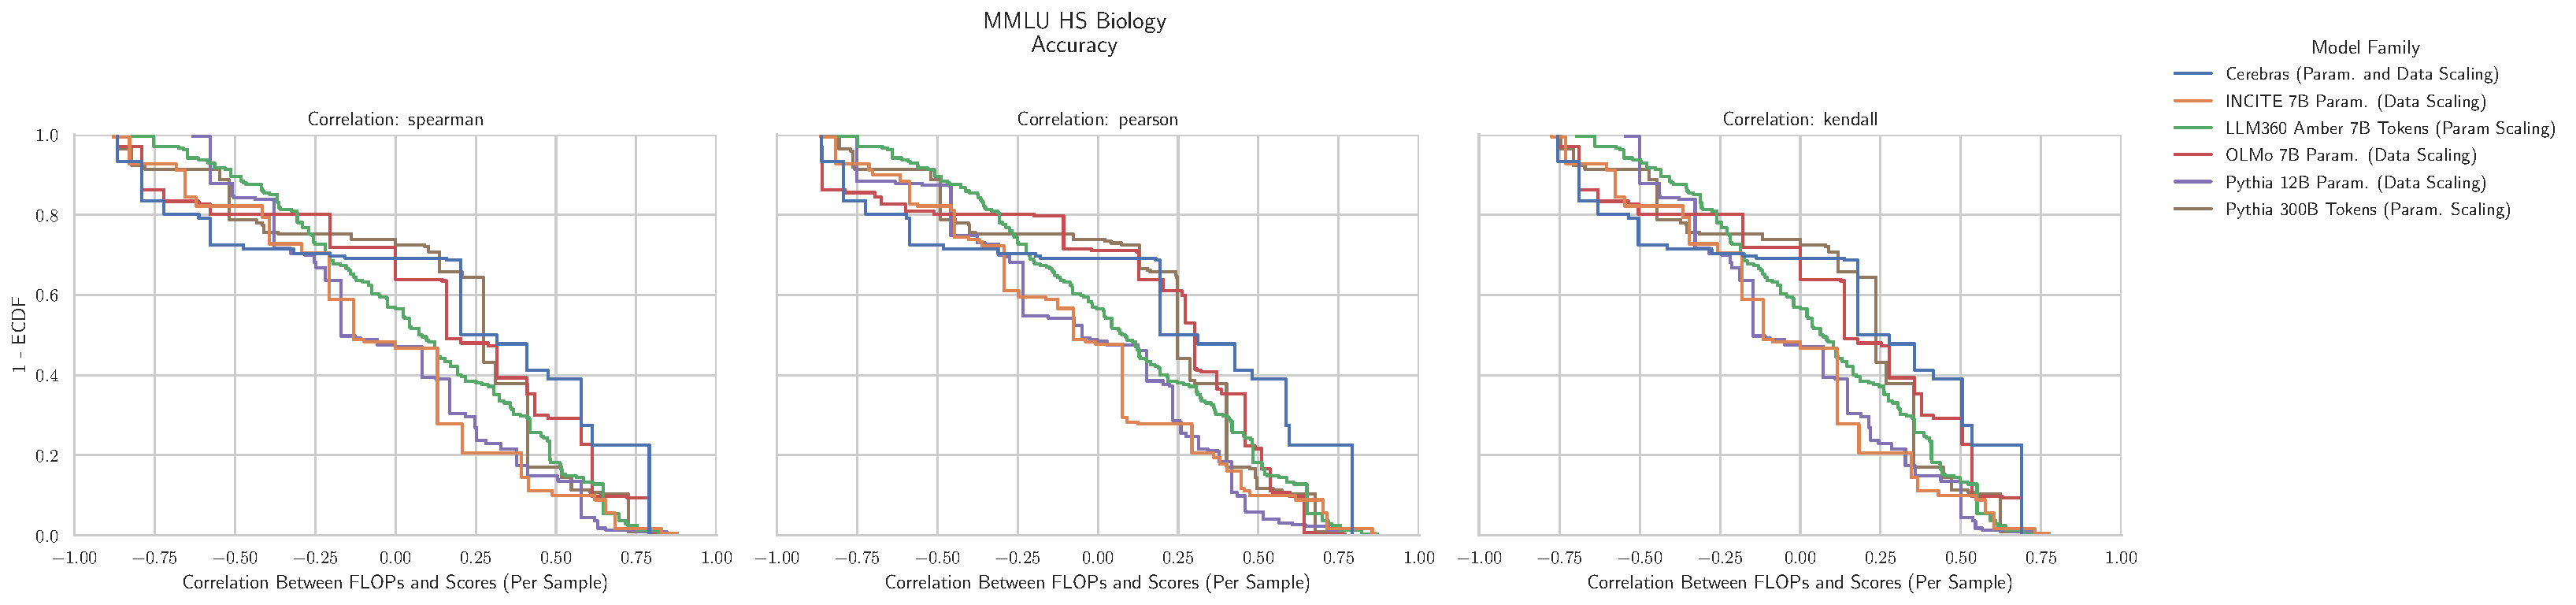
\includegraphics[width=\textwidth]{figures/correlations_between_scores_and_compute/correlation_distributions/mmlu_high_school_biology/mmlu_high_school_biology_acc_ecdf_vs_correlation_score_by_modelfamily_split_correlation_metric.pdf}
    \caption{\textbf{MMLU High School Biology: Downstream performance is computed via a sequence of transformations that deteriorate correlations between scores and pretraining compute.}}
    \label{app:fig:compute_score_distribution_mmlu_high_school_biology}
\end{figure}


\clearpage
\subsection{NLP Benchmark: MMLU High School Chemistry \cite{hendrycks2020mmlu}}

\begin{figure}[h!]
    \centering
    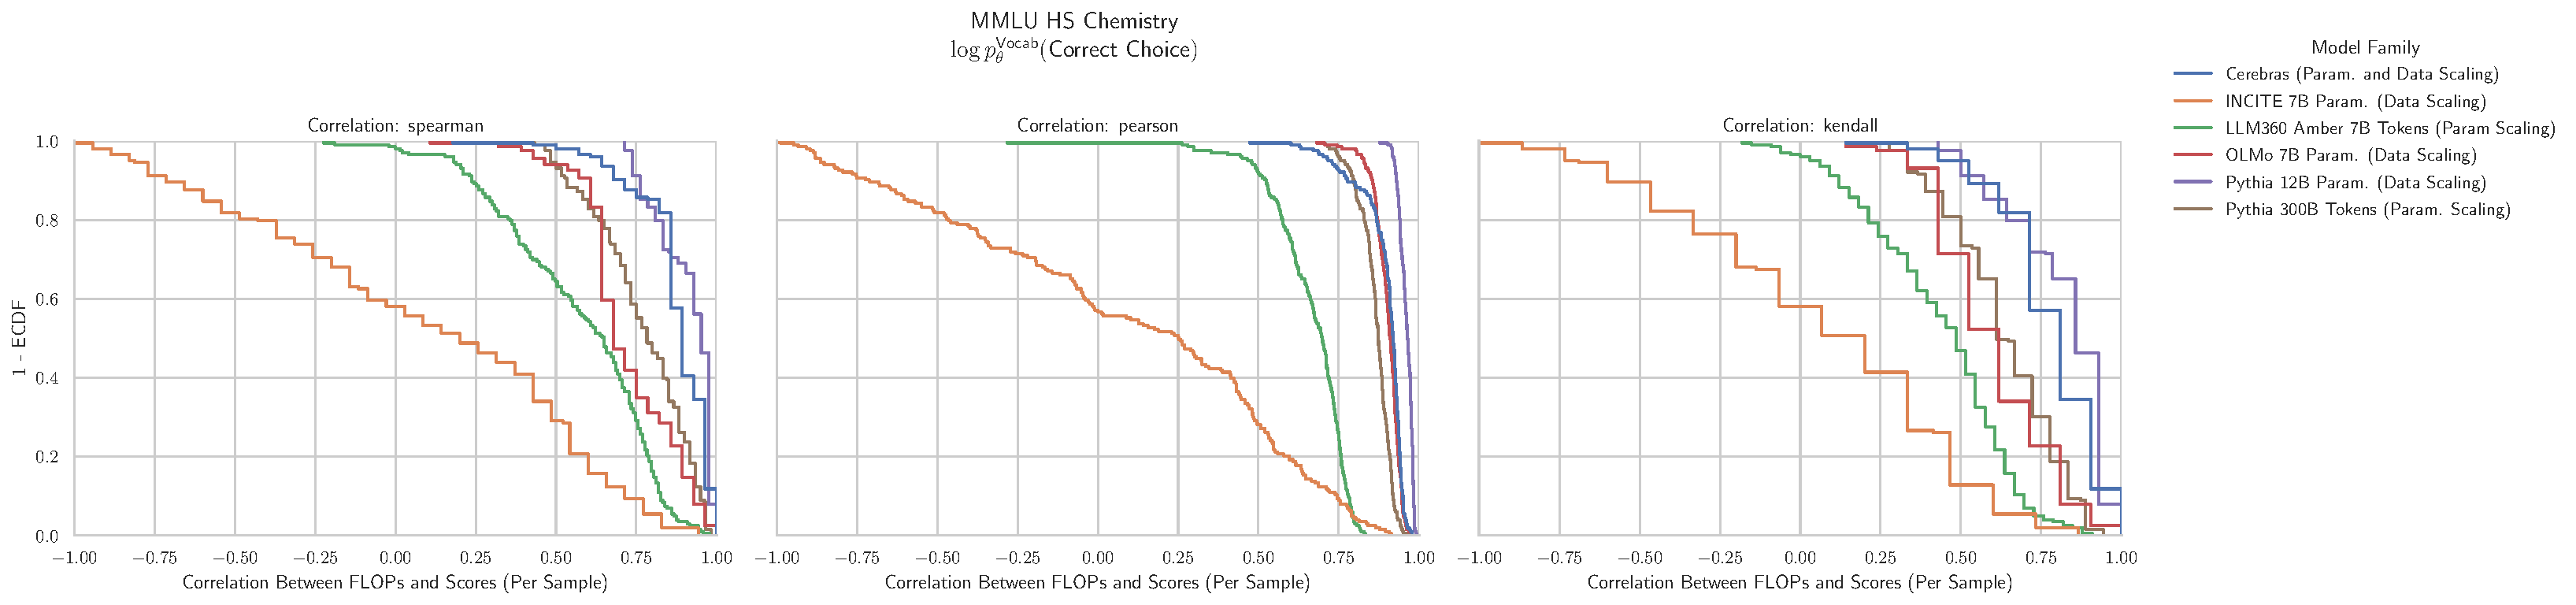
\includegraphics[width=\textwidth]{figures/correlations_between_scores_and_compute/correlation_distributions/mmlu_high_school_chemistry/mmlu_high_school_chemistry_log_likelihood_correct_ecdf_vs_correlation_score_by_modelfamily_split_correlation_metric.pdf}
    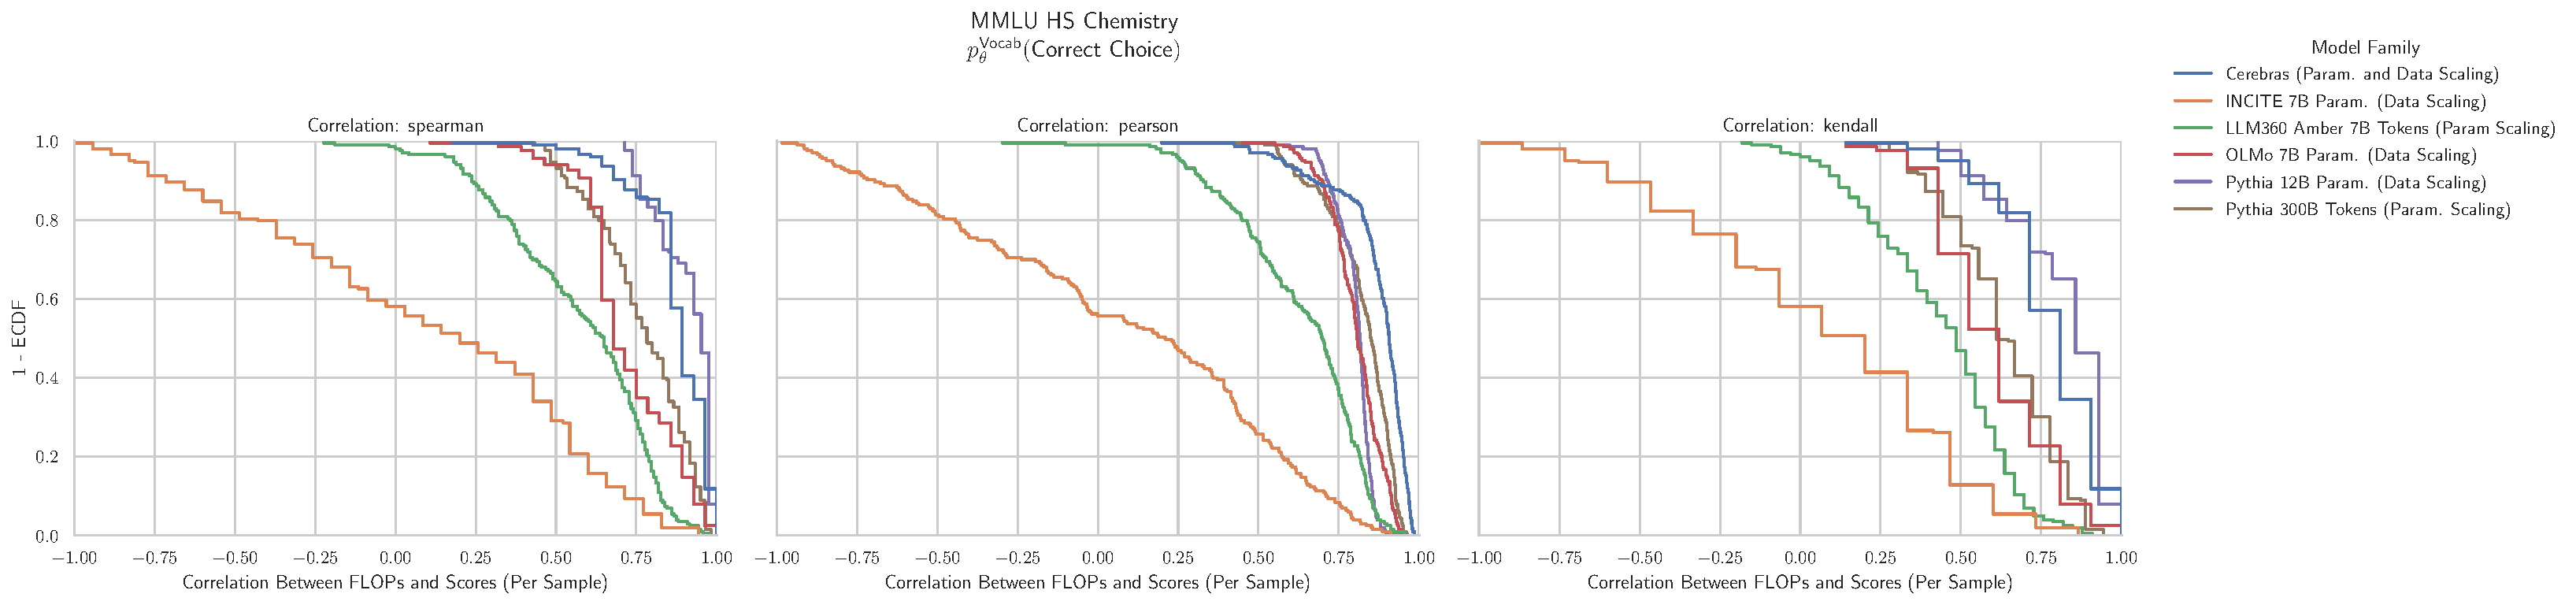
\includegraphics[width=\textwidth]{figures/correlations_between_scores_and_compute/correlation_distributions/mmlu_high_school_chemistry/mmlu_high_school_chemistry_prob_correct_vocab_ecdf_vs_correlation_score_by_modelfamily_split_correlation_metric.pdf}
    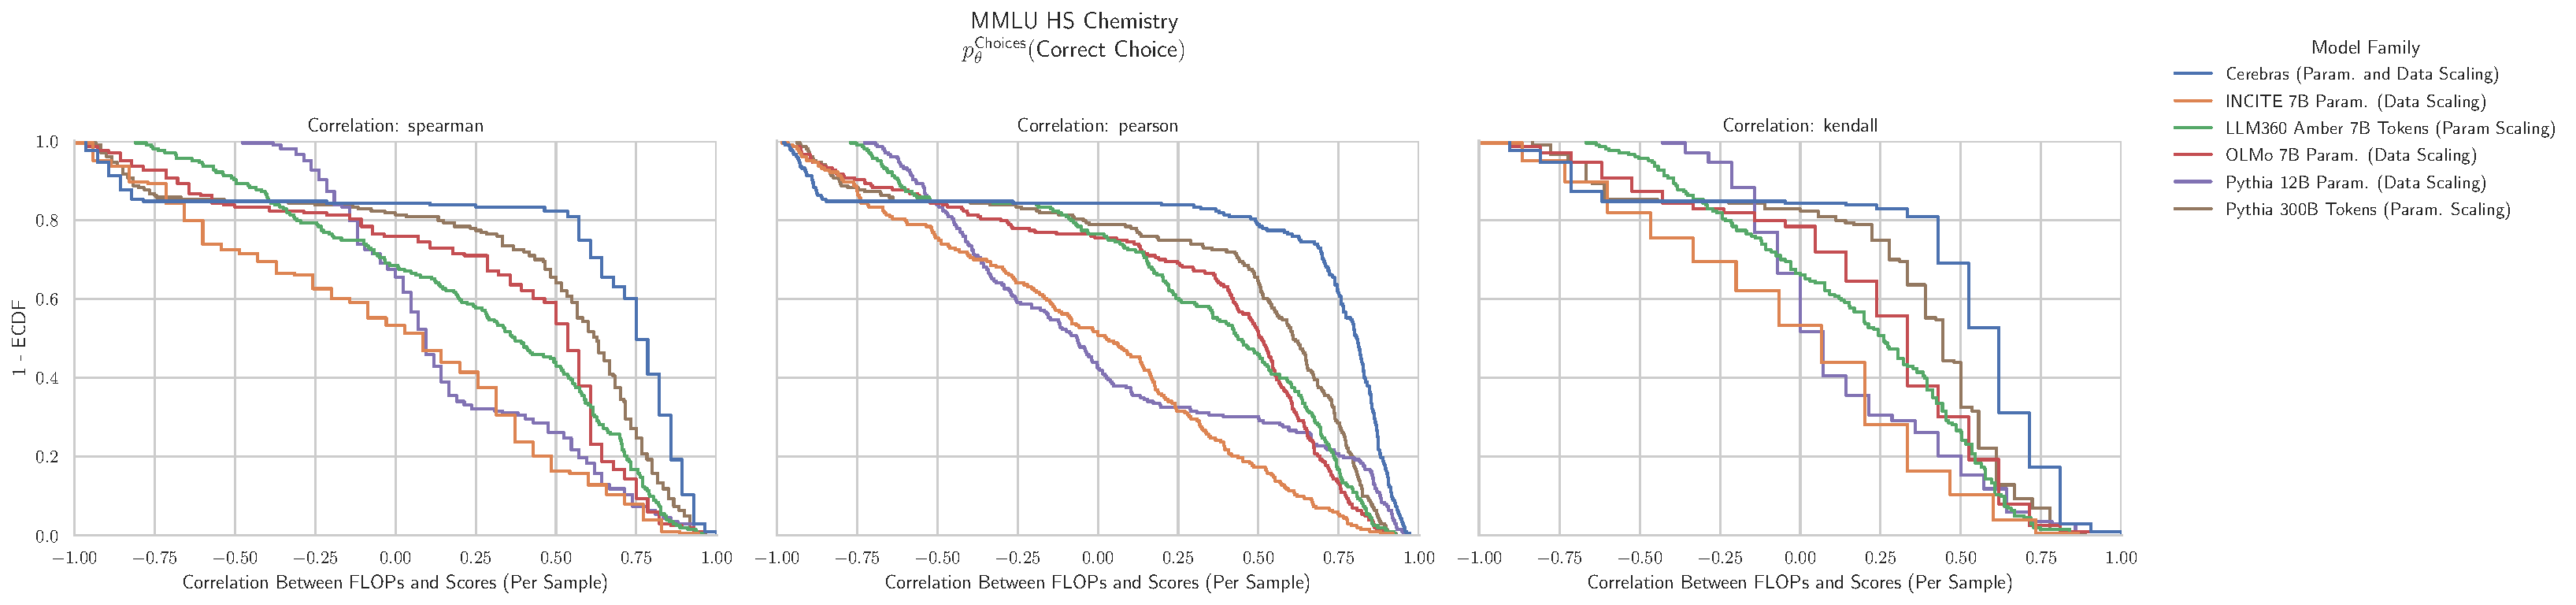
\includegraphics[width=\textwidth]{figures/correlations_between_scores_and_compute/correlation_distributions/mmlu_high_school_chemistry/mmlu_high_school_chemistry_prob_correct_choices_ecdf_vs_correlation_score_by_modelfamily_split_correlation_metric.pdf}
    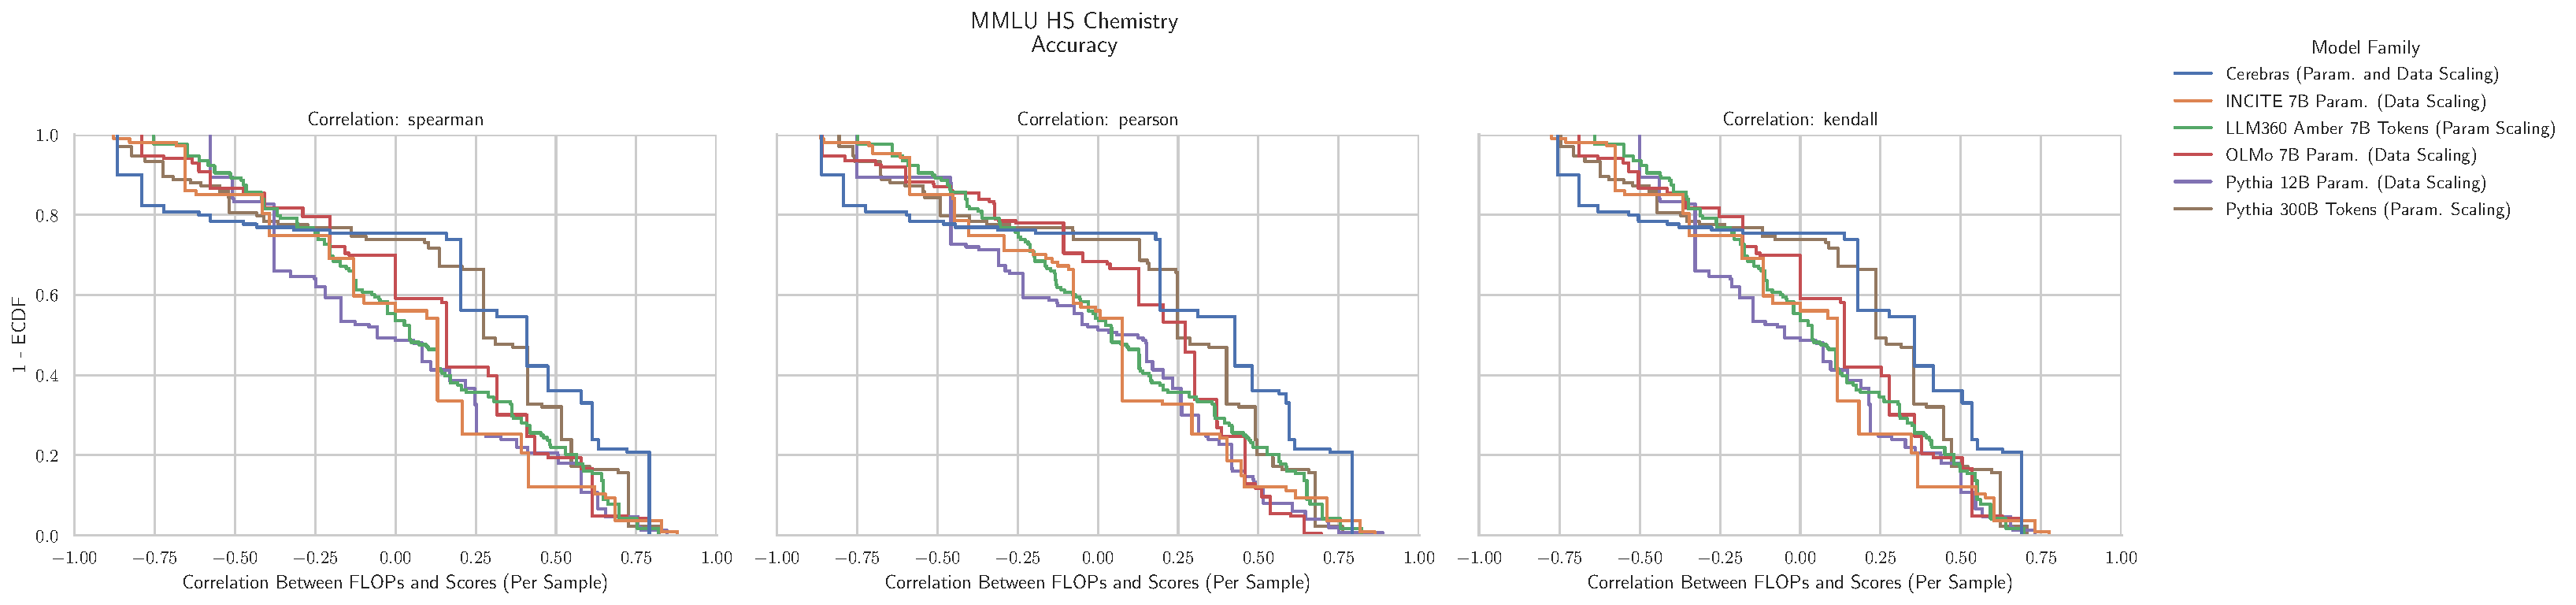
\includegraphics[width=\textwidth]{figures/correlations_between_scores_and_compute/correlation_distributions/mmlu_high_school_chemistry/mmlu_high_school_chemistry_acc_ecdf_vs_correlation_score_by_modelfamily_split_correlation_metric.pdf}
    \caption{\textbf{MMLU High School Chemistry: Downstream performance is computed via a sequence of transformations that deteriorate correlations between scores and pretraining compute.}}
    \label{app:fig:compute_score_distribution_mmlu_high_school_chemistry}
\end{figure}


\clearpage
\subsection{NLP Benchmark: MMLU High School Computer Science \cite{hendrycks2020mmlu}}

\begin{figure}[h!]
    \centering
    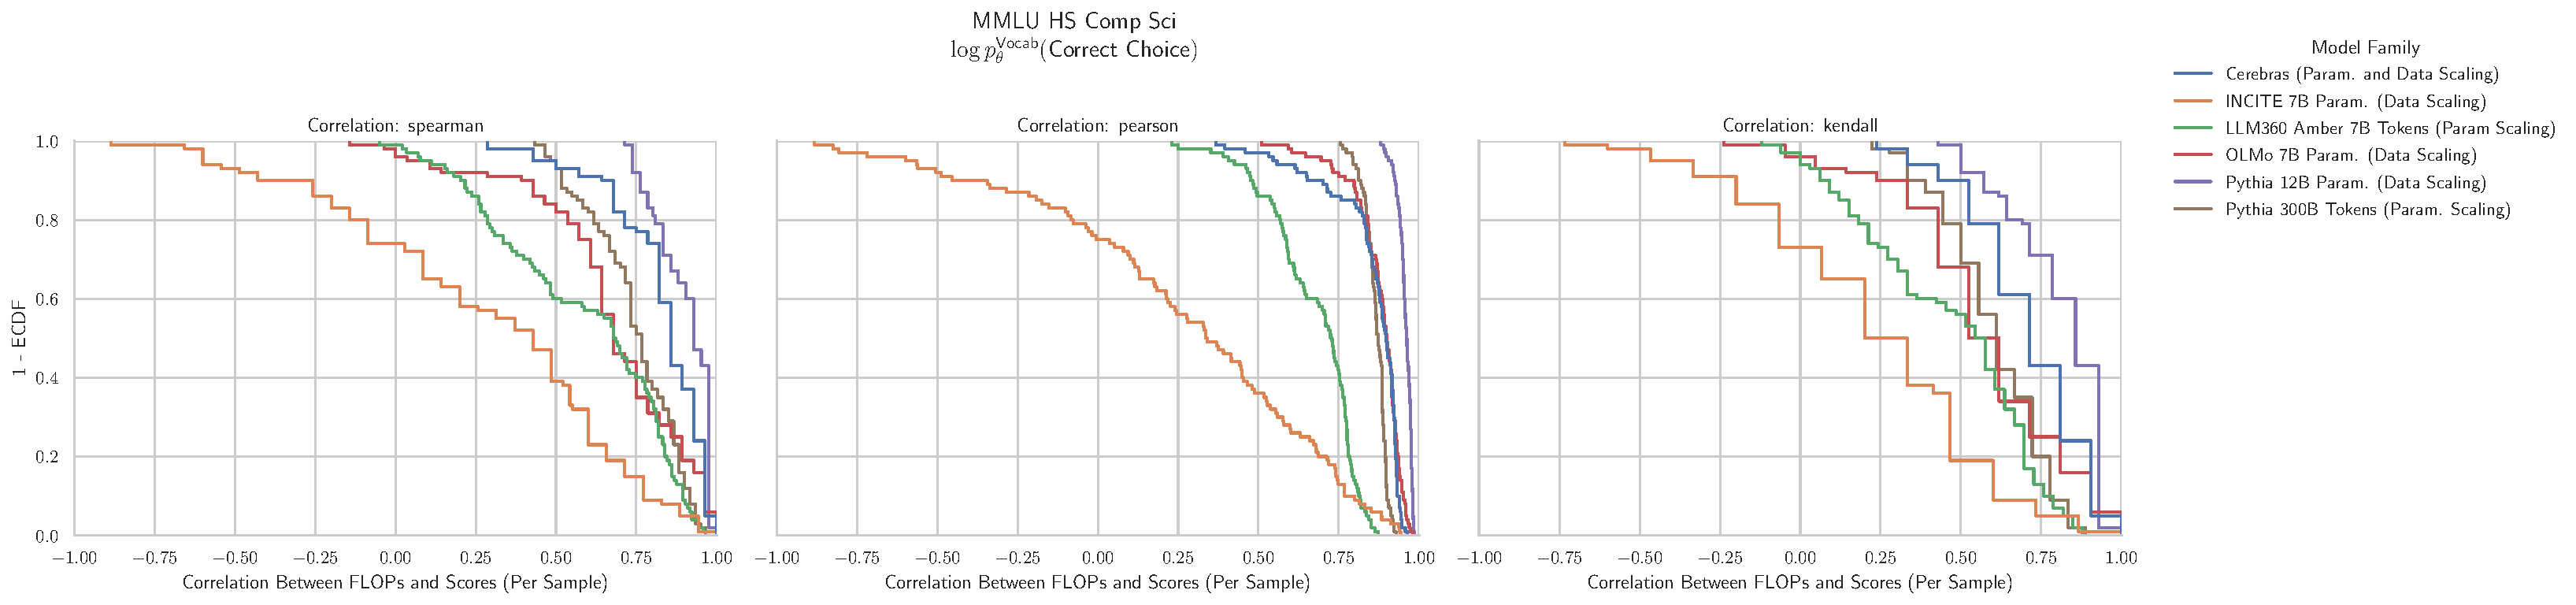
\includegraphics[width=\textwidth]{figures/correlations_between_scores_and_compute/correlation_distributions/mmlu_high_school_computer_science/mmlu_high_school_computer_science_log_likelihood_correct_ecdf_vs_correlation_score_by_modelfamily_split_correlation_metric.pdf}
    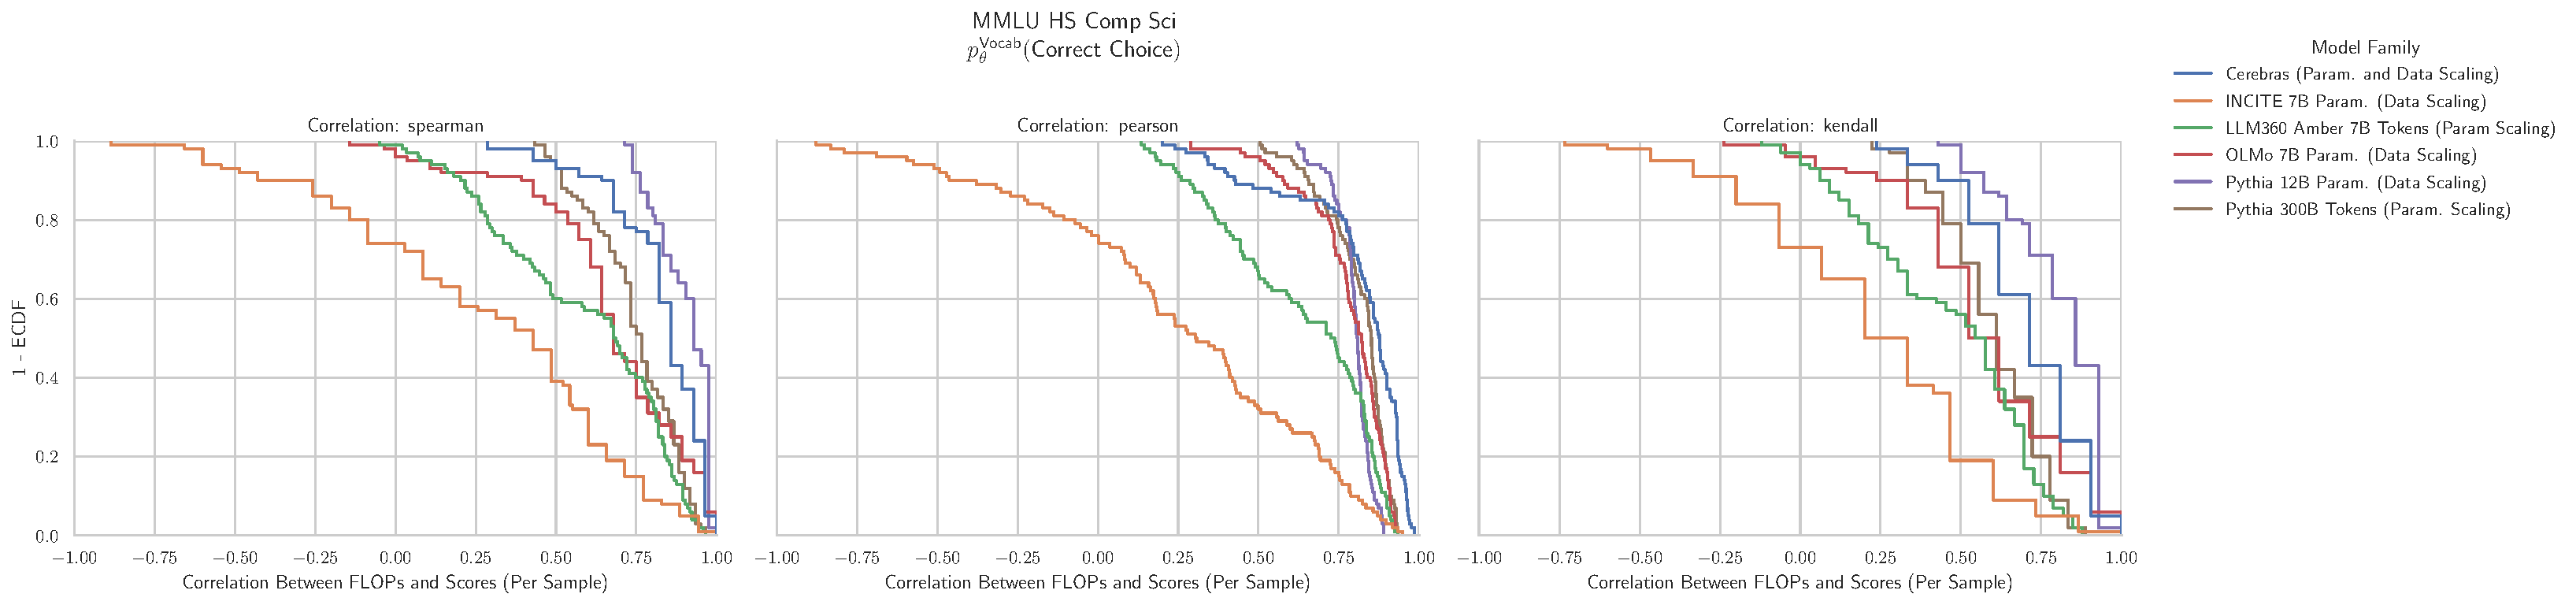
\includegraphics[width=\textwidth]{figures/correlations_between_scores_and_compute/correlation_distributions/mmlu_high_school_computer_science/mmlu_high_school_computer_science_prob_correct_vocab_ecdf_vs_correlation_score_by_modelfamily_split_correlation_metric.pdf}
    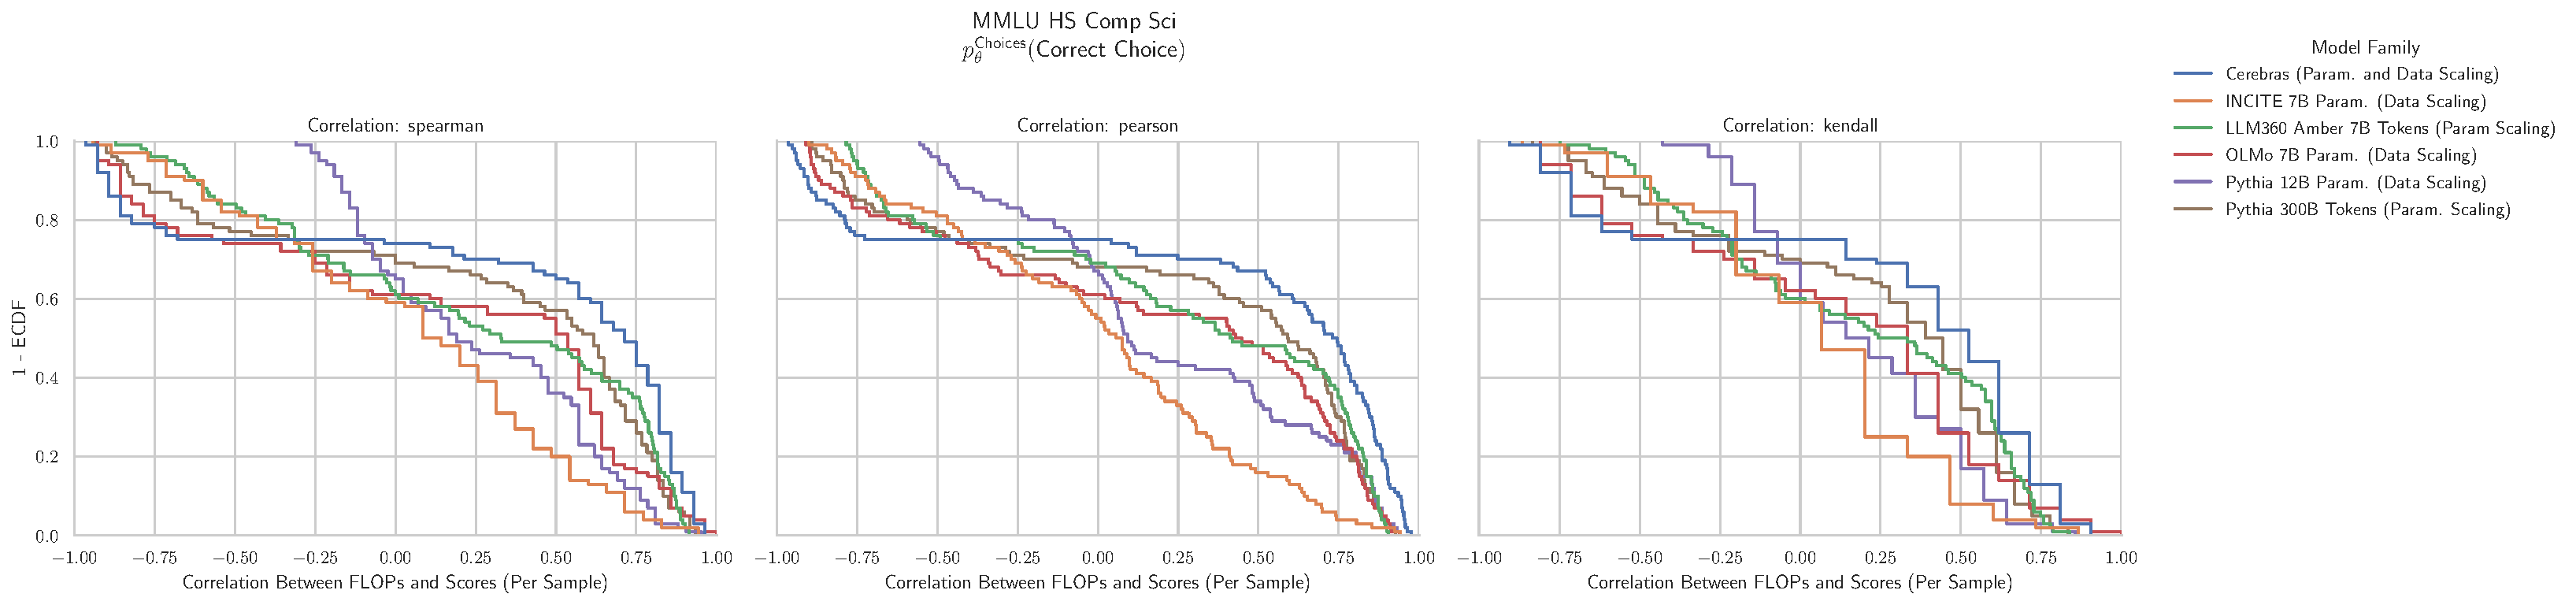
\includegraphics[width=\textwidth]{figures/correlations_between_scores_and_compute/correlation_distributions/mmlu_high_school_computer_science/mmlu_high_school_computer_science_prob_correct_choices_ecdf_vs_correlation_score_by_modelfamily_split_correlation_metric.pdf}
    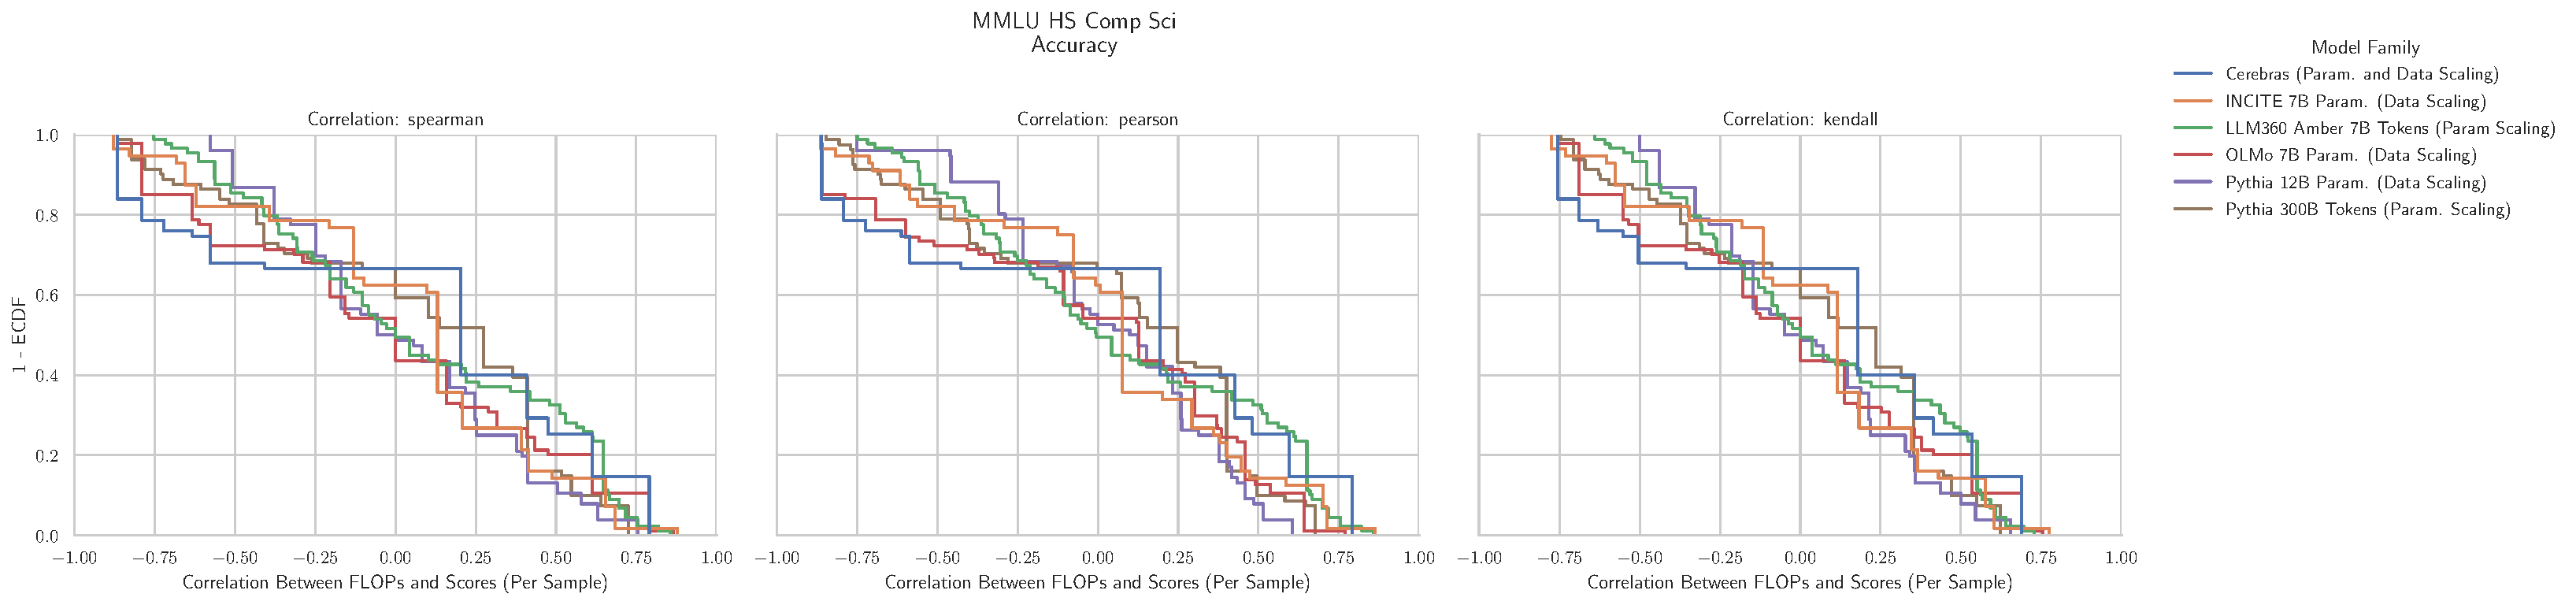
\includegraphics[width=\textwidth]{figures/correlations_between_scores_and_compute/correlation_distributions/mmlu_high_school_computer_science/mmlu_high_school_computer_science_acc_ecdf_vs_correlation_score_by_modelfamily_split_correlation_metric.pdf}
    \caption{\textbf{MMLU High School Computer Science: Downstream performance is computed via a sequence of transformations that deteriorate correlations between scores and pretraining compute.}}
    \label{app:fig:compute_score_distribution_mmlu_high_school_computer_science}
\end{figure}


\clearpage
\subsection{NLP Benchmark: MMLU High School Chemistry \cite{hendrycks2020mmlu}}

\begin{figure}[h!]
    \centering
    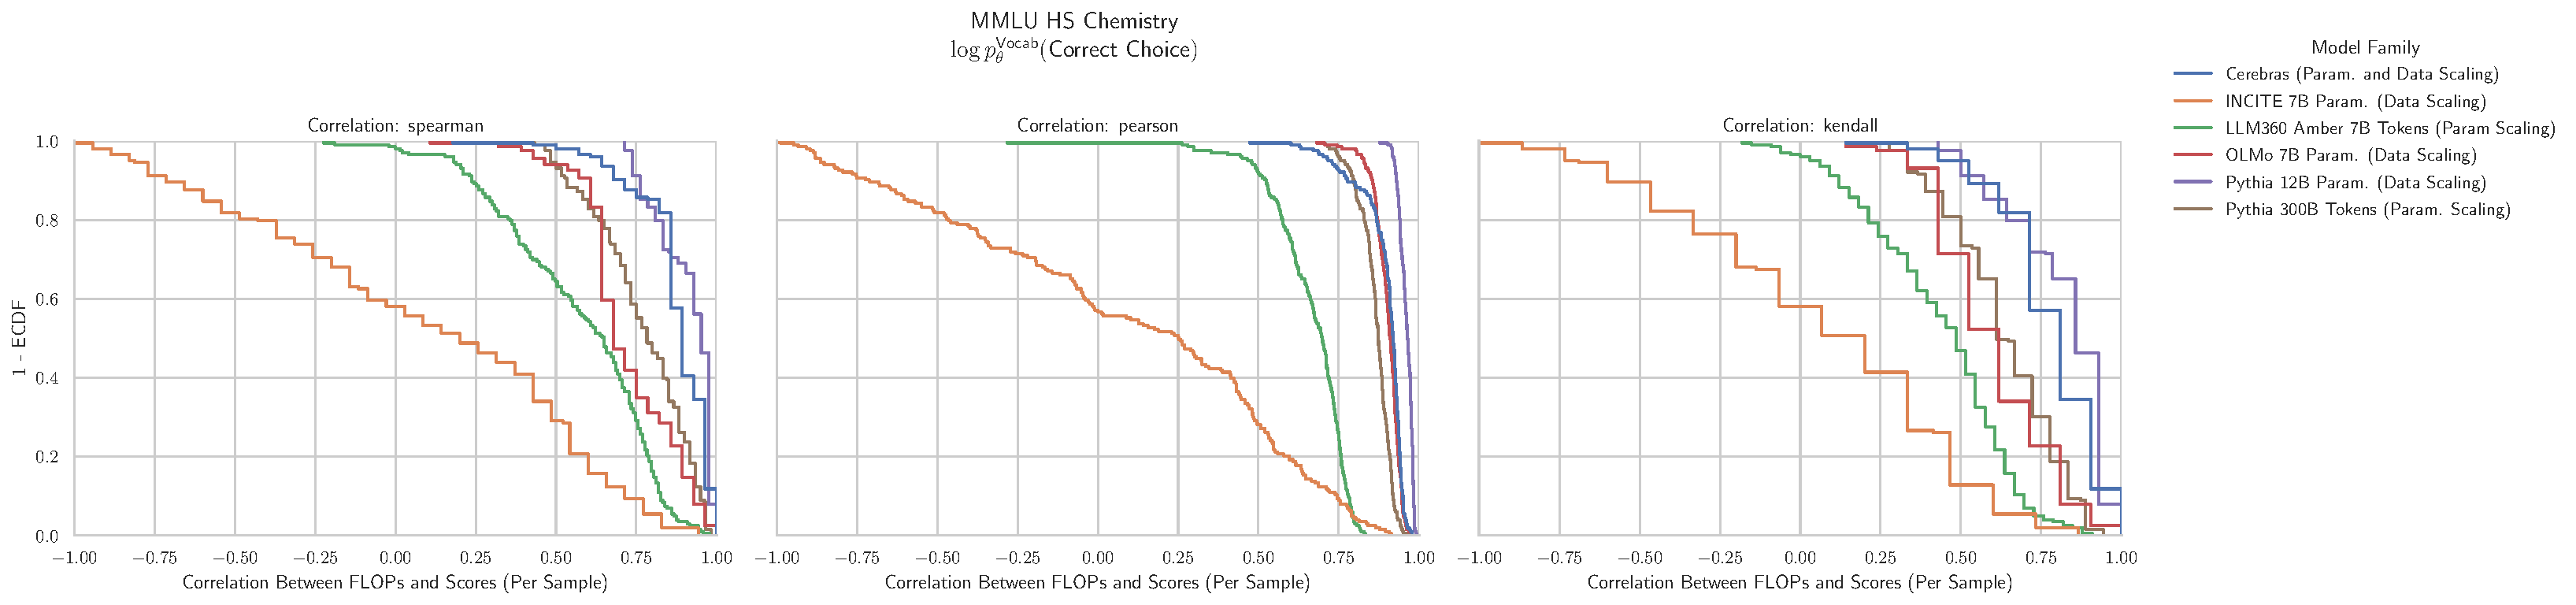
\includegraphics[width=\textwidth]{figures/correlations_between_scores_and_compute/correlation_distributions/mmlu_high_school_chemistry/mmlu_high_school_chemistry_log_likelihood_correct_ecdf_vs_correlation_score_by_modelfamily_split_correlation_metric.pdf}
    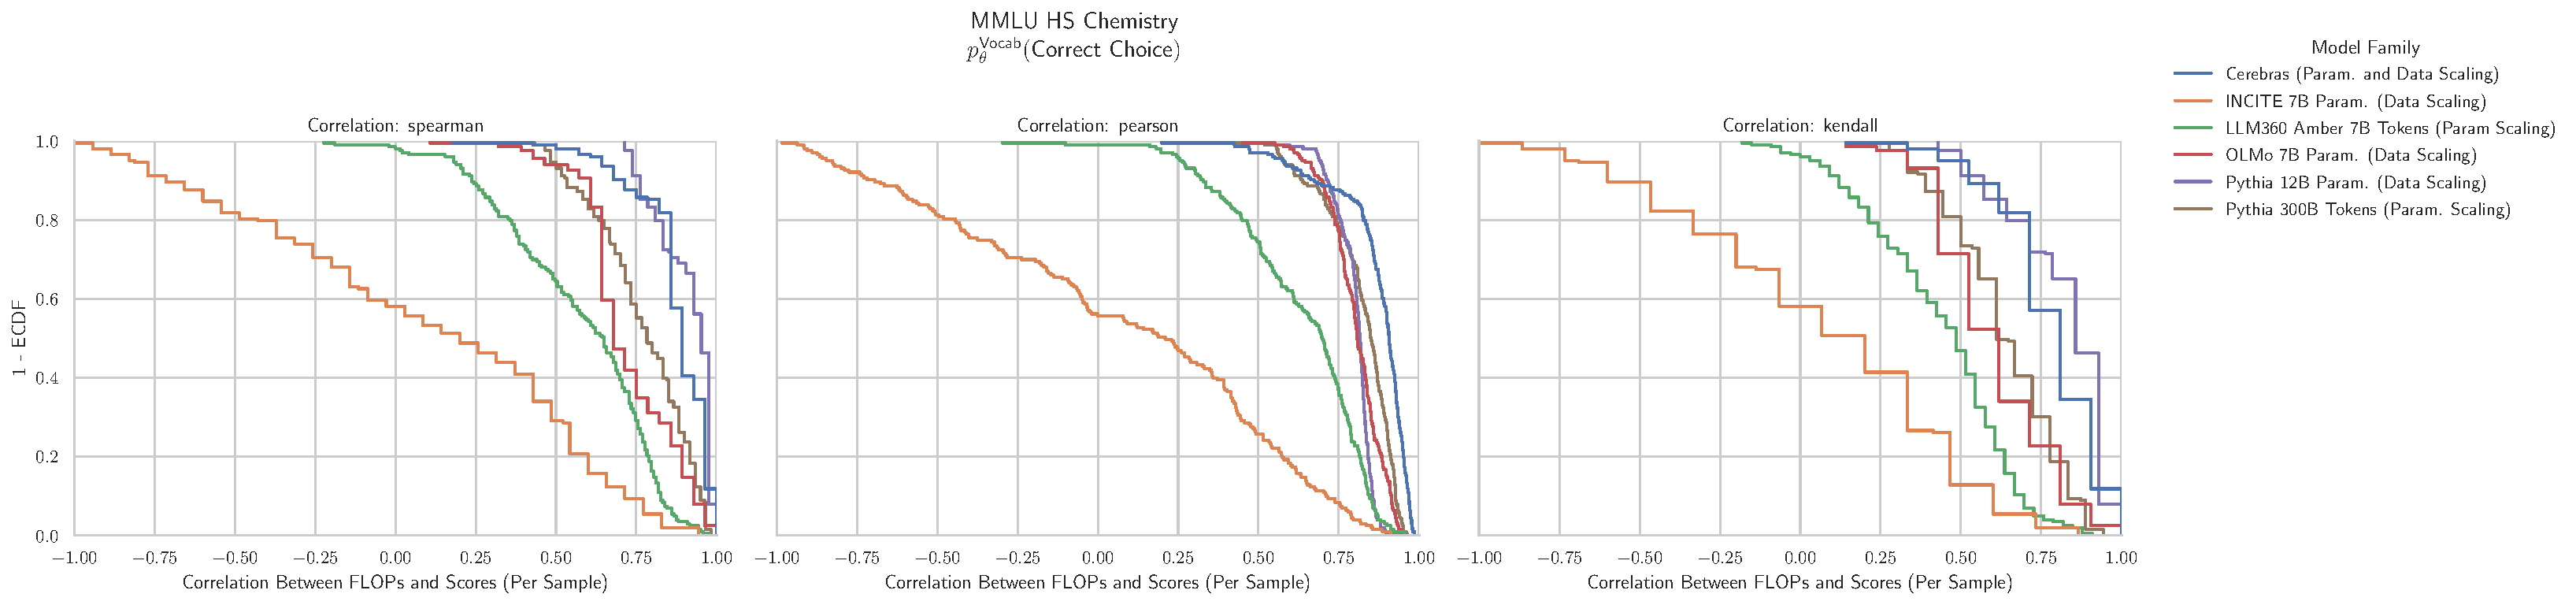
\includegraphics[width=\textwidth]{figures/correlations_between_scores_and_compute/correlation_distributions/mmlu_high_school_chemistry/mmlu_high_school_chemistry_prob_correct_vocab_ecdf_vs_correlation_score_by_modelfamily_split_correlation_metric.pdf}
    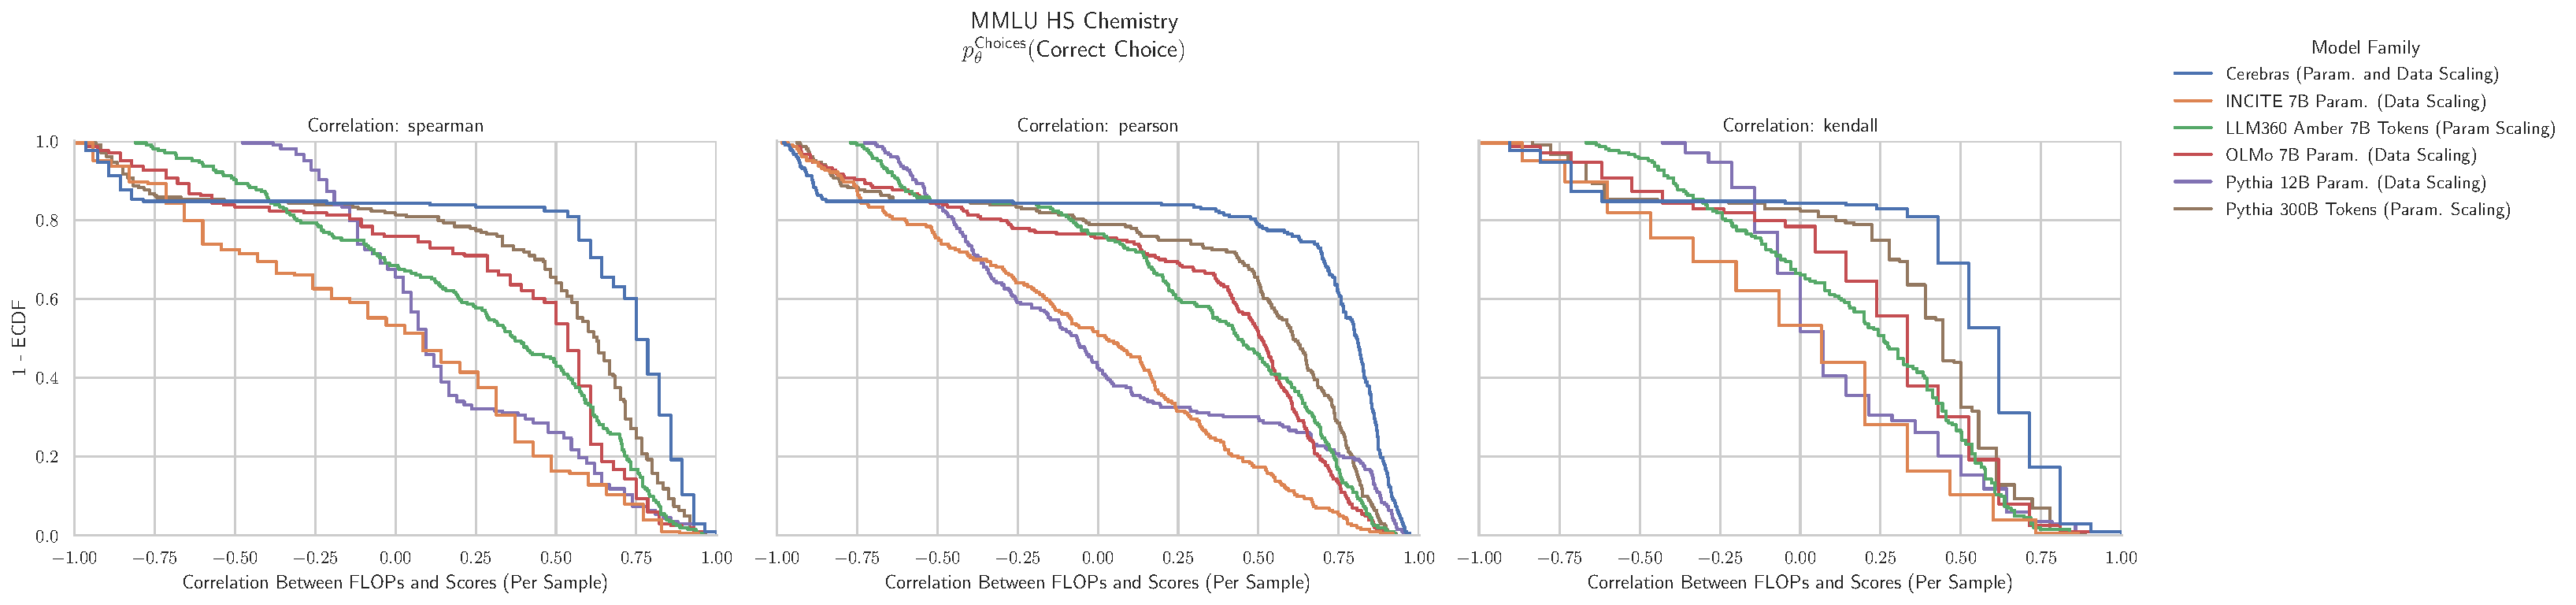
\includegraphics[width=\textwidth]{figures/correlations_between_scores_and_compute/correlation_distributions/mmlu_high_school_chemistry/mmlu_high_school_chemistry_prob_correct_choices_ecdf_vs_correlation_score_by_modelfamily_split_correlation_metric.pdf}
    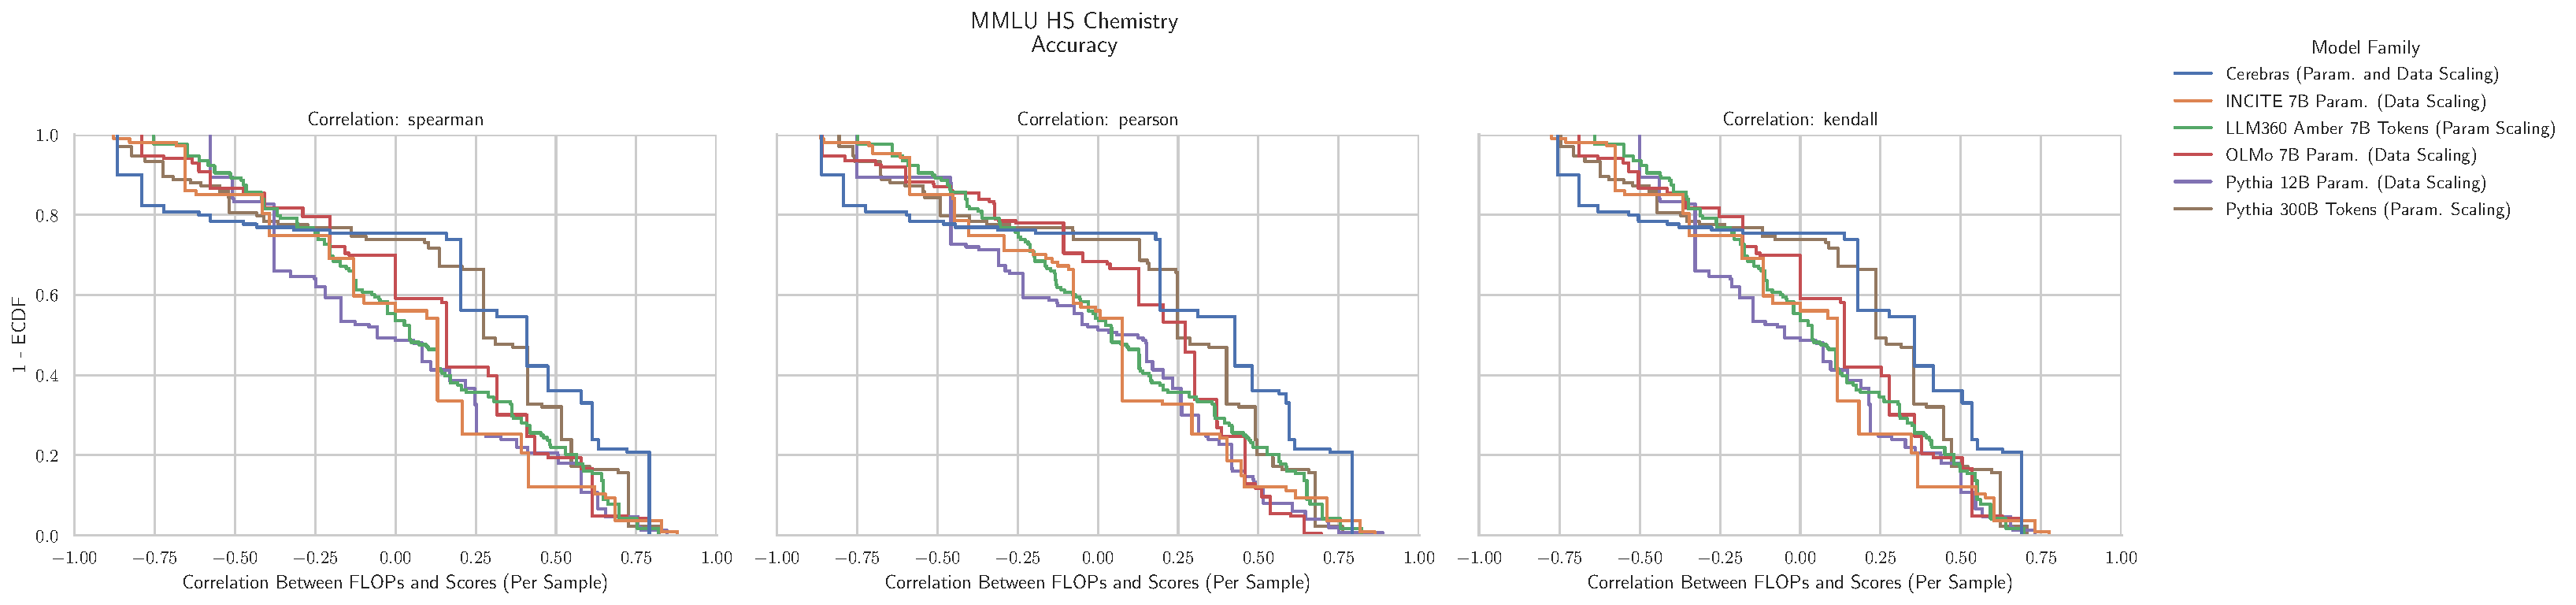
\includegraphics[width=\textwidth]{figures/correlations_between_scores_and_compute/correlation_distributions/mmlu_high_school_chemistry/mmlu_high_school_chemistry_acc_ecdf_vs_correlation_score_by_modelfamily_split_correlation_metric.pdf}
    \caption{\textbf{MMLU High School Chemistry: Downstream performance is computed via a sequence of transformations that deteriorate correlations between scores and pretraining compute.}}
    \label{app:fig:compute_score_distribution_mmlu_high_school_chemistry}
\end{figure}


\clearpage
\subsection{NLP Benchmark: MMLU High School European History \cite{hendrycks2020mmlu}}

\begin{figure}[h!]
    \centering
    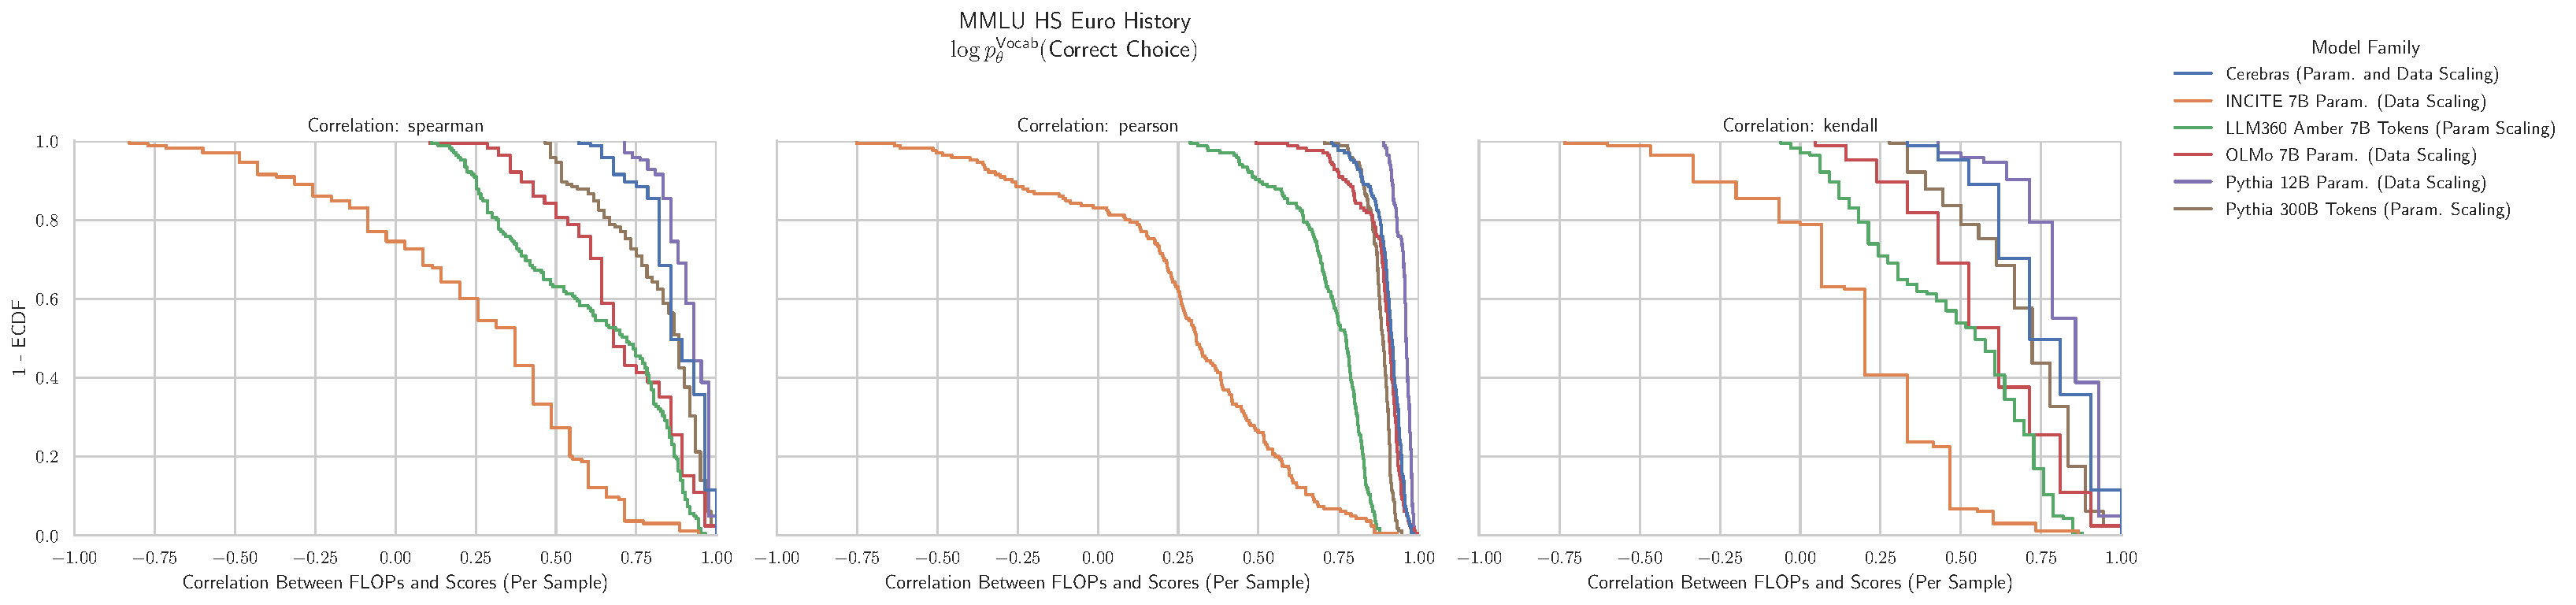
\includegraphics[width=\textwidth]{figures/correlations_between_scores_and_compute/correlation_distributions/mmlu_high_school_european_history/mmlu_high_school_european_history_log_likelihood_correct_ecdf_vs_correlation_score_by_modelfamily_split_correlation_metric.pdf}
    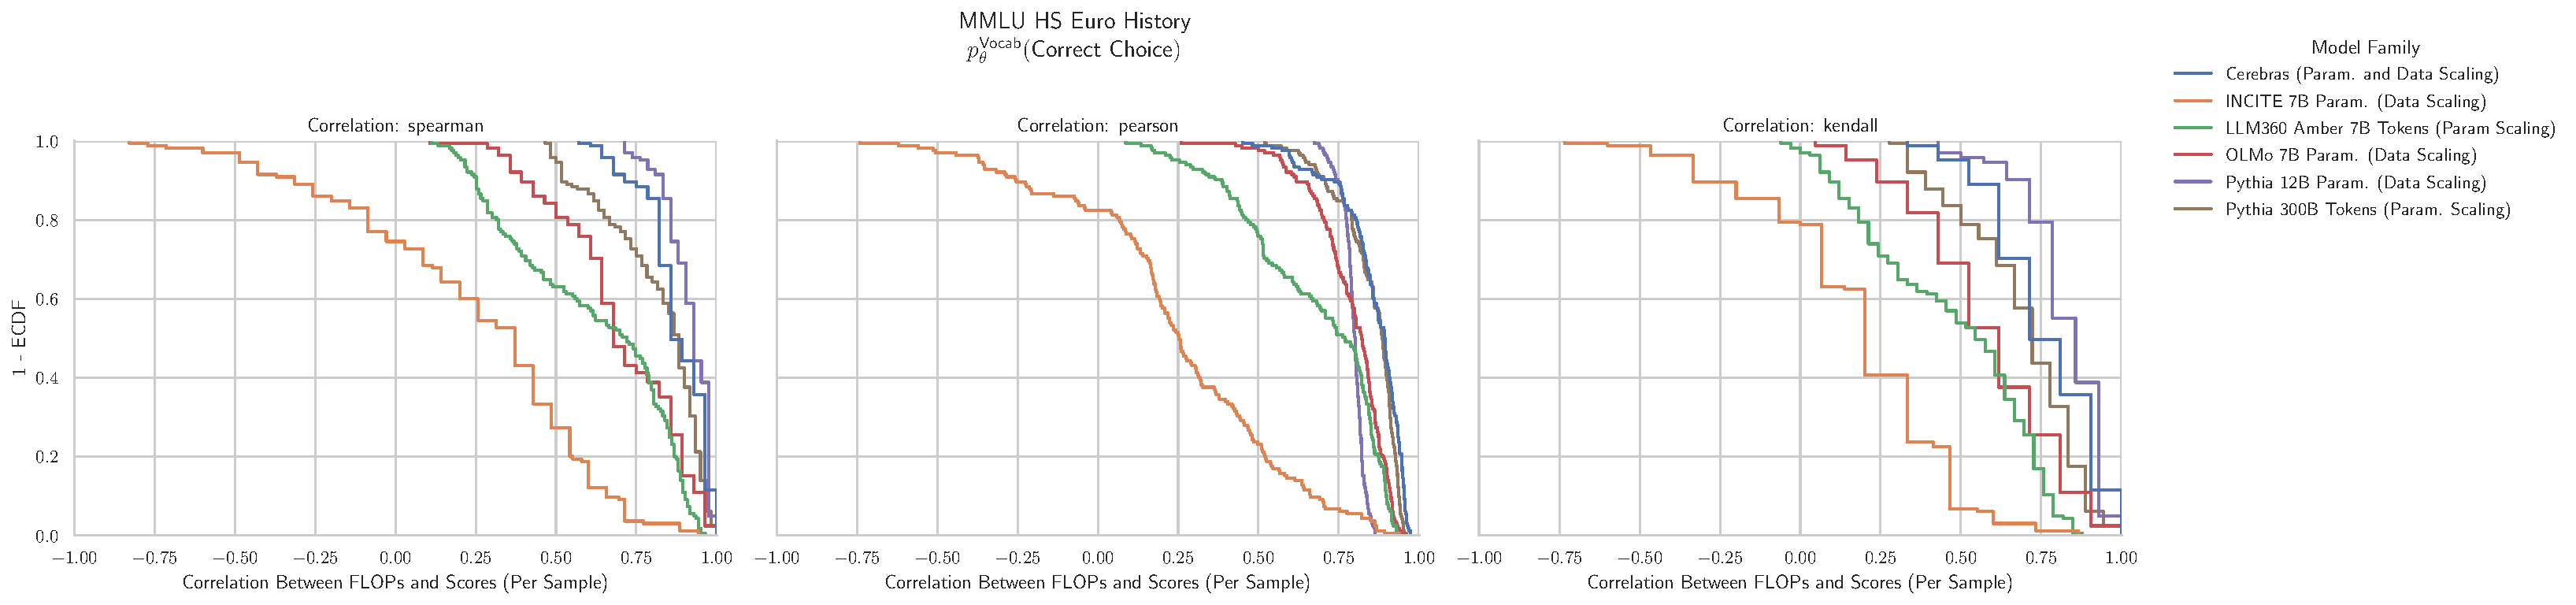
\includegraphics[width=\textwidth]{figures/correlations_between_scores_and_compute/correlation_distributions/mmlu_high_school_european_history/mmlu_high_school_european_history_prob_correct_vocab_ecdf_vs_correlation_score_by_modelfamily_split_correlation_metric.pdf}
    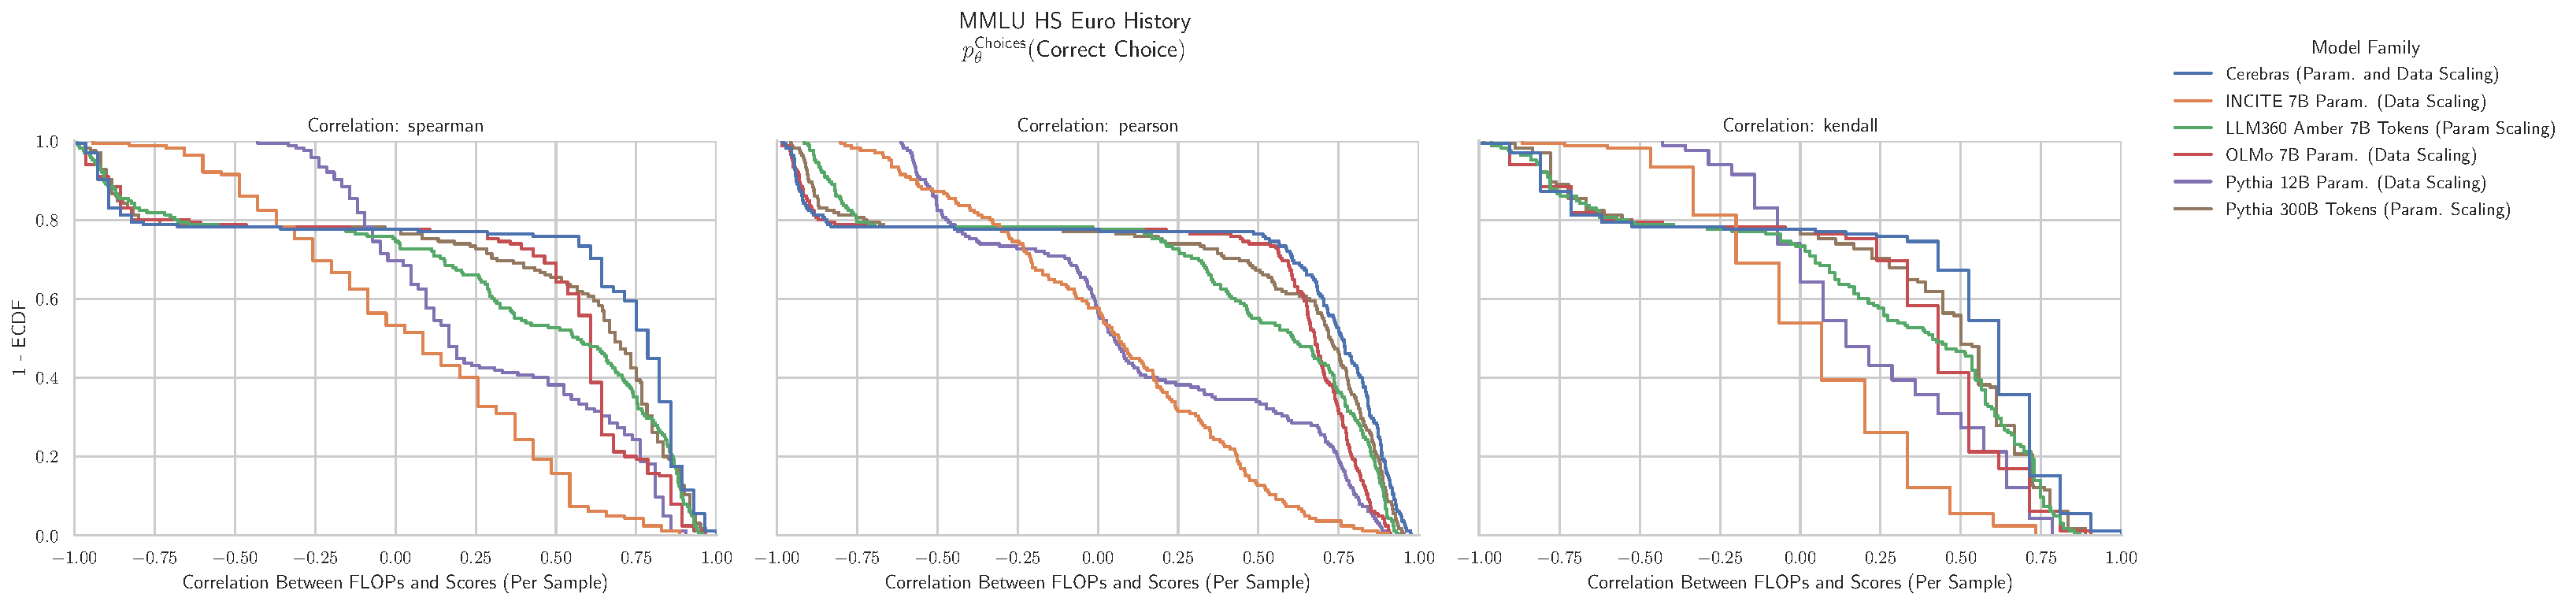
\includegraphics[width=\textwidth]{figures/correlations_between_scores_and_compute/correlation_distributions/mmlu_high_school_european_history/mmlu_high_school_european_history_prob_correct_choices_ecdf_vs_correlation_score_by_modelfamily_split_correlation_metric.pdf}
    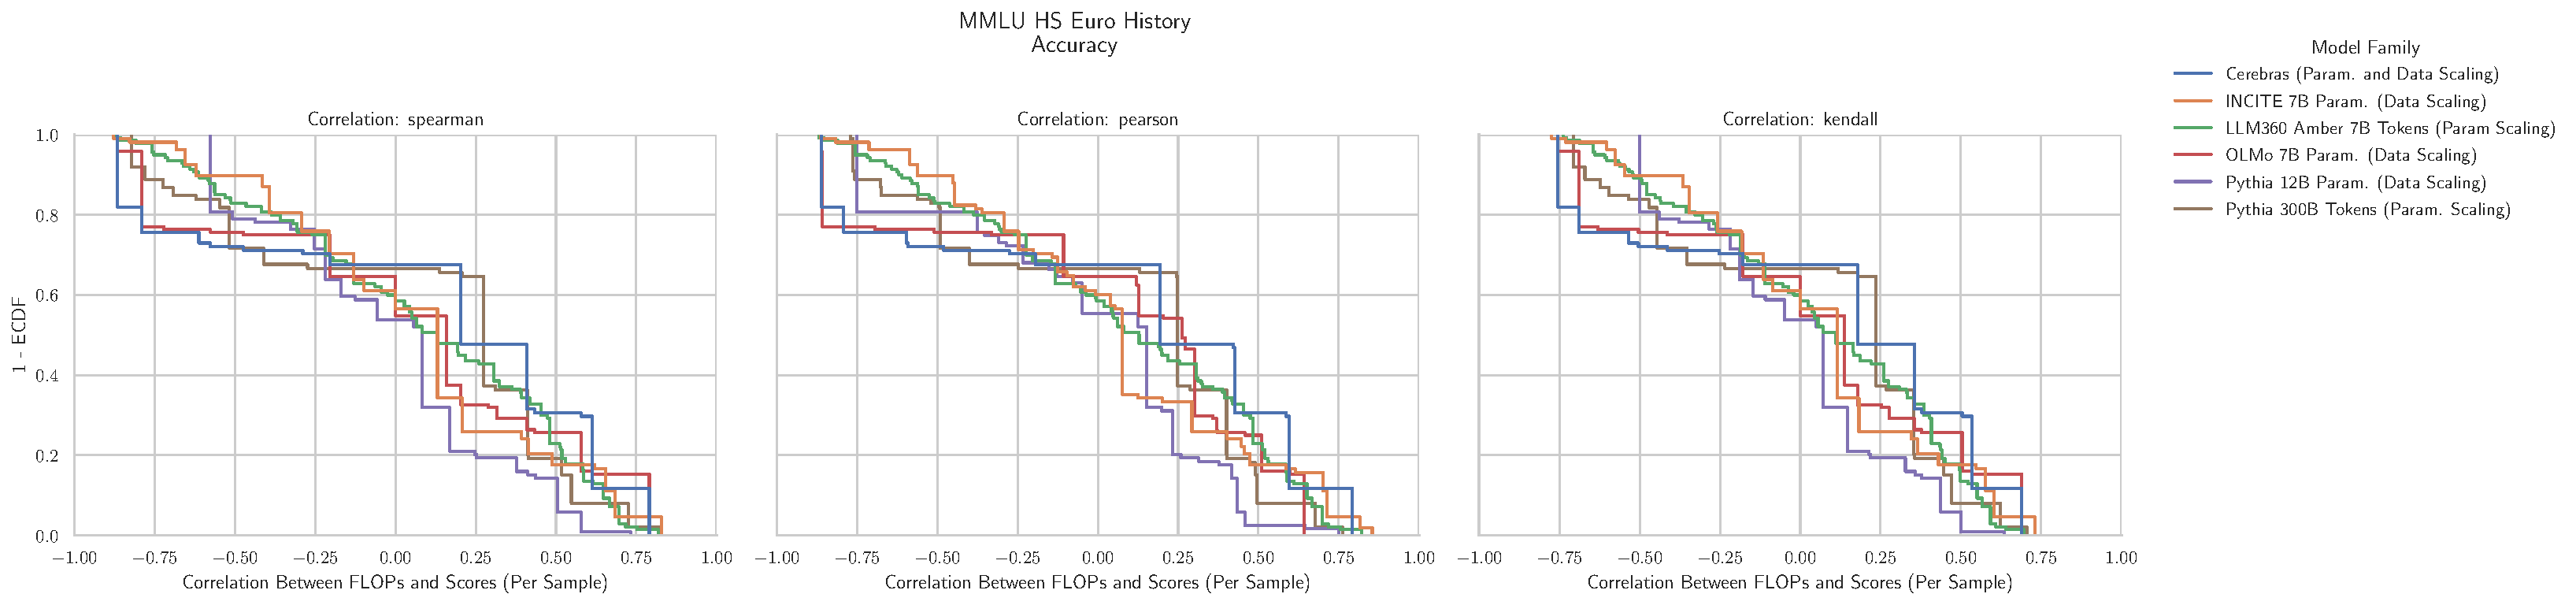
\includegraphics[width=\textwidth]{figures/correlations_between_scores_and_compute/correlation_distributions/mmlu_high_school_european_history/mmlu_high_school_european_history_acc_ecdf_vs_correlation_score_by_modelfamily_split_correlation_metric.pdf}
    \caption{\textbf{MMLU High School European History: Downstream performance is computed via a sequence of transformations that deteriorate correlations between scores and pretraining compute.}}
    \label{app:fig:compute_score_distribution_mmlu_high_school_european_history}
\end{figure}


\clearpage
\subsection{NLP Benchmark: MMLU High School Geography \cite{hendrycks2020mmlu}}

\begin{figure}[h!]
    \centering
    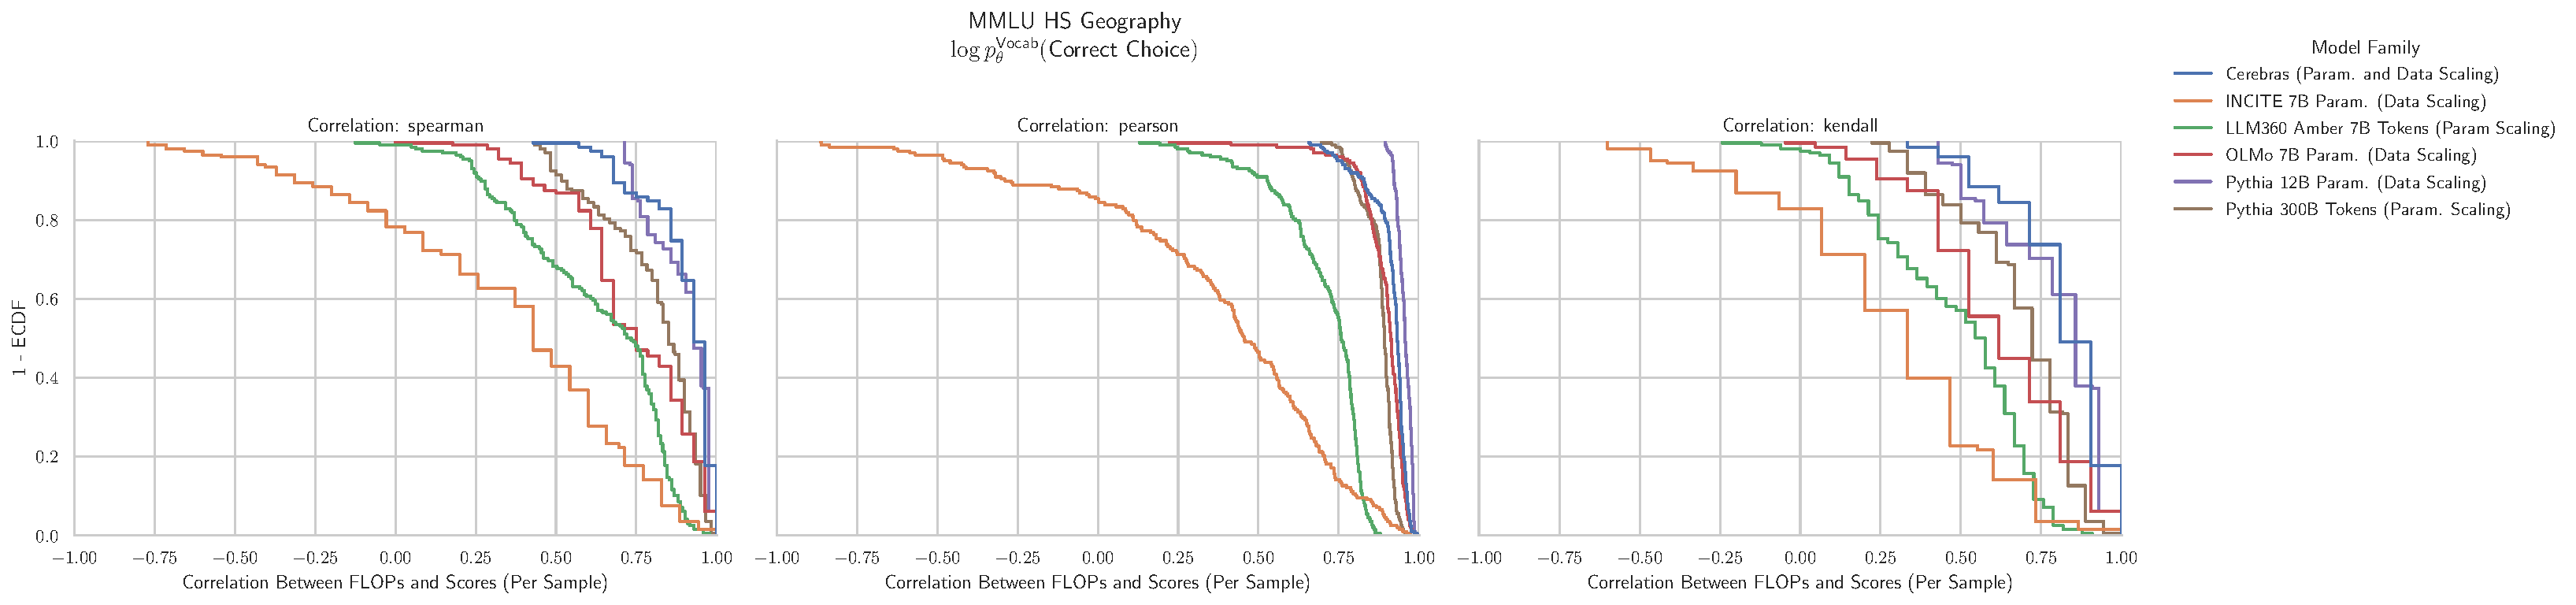
\includegraphics[width=\textwidth]{figures/correlations_between_scores_and_compute/correlation_distributions/mmlu_high_school_geography/mmlu_high_school_geography_log_likelihood_correct_ecdf_vs_correlation_score_by_modelfamily_split_correlation_metric.pdf}
    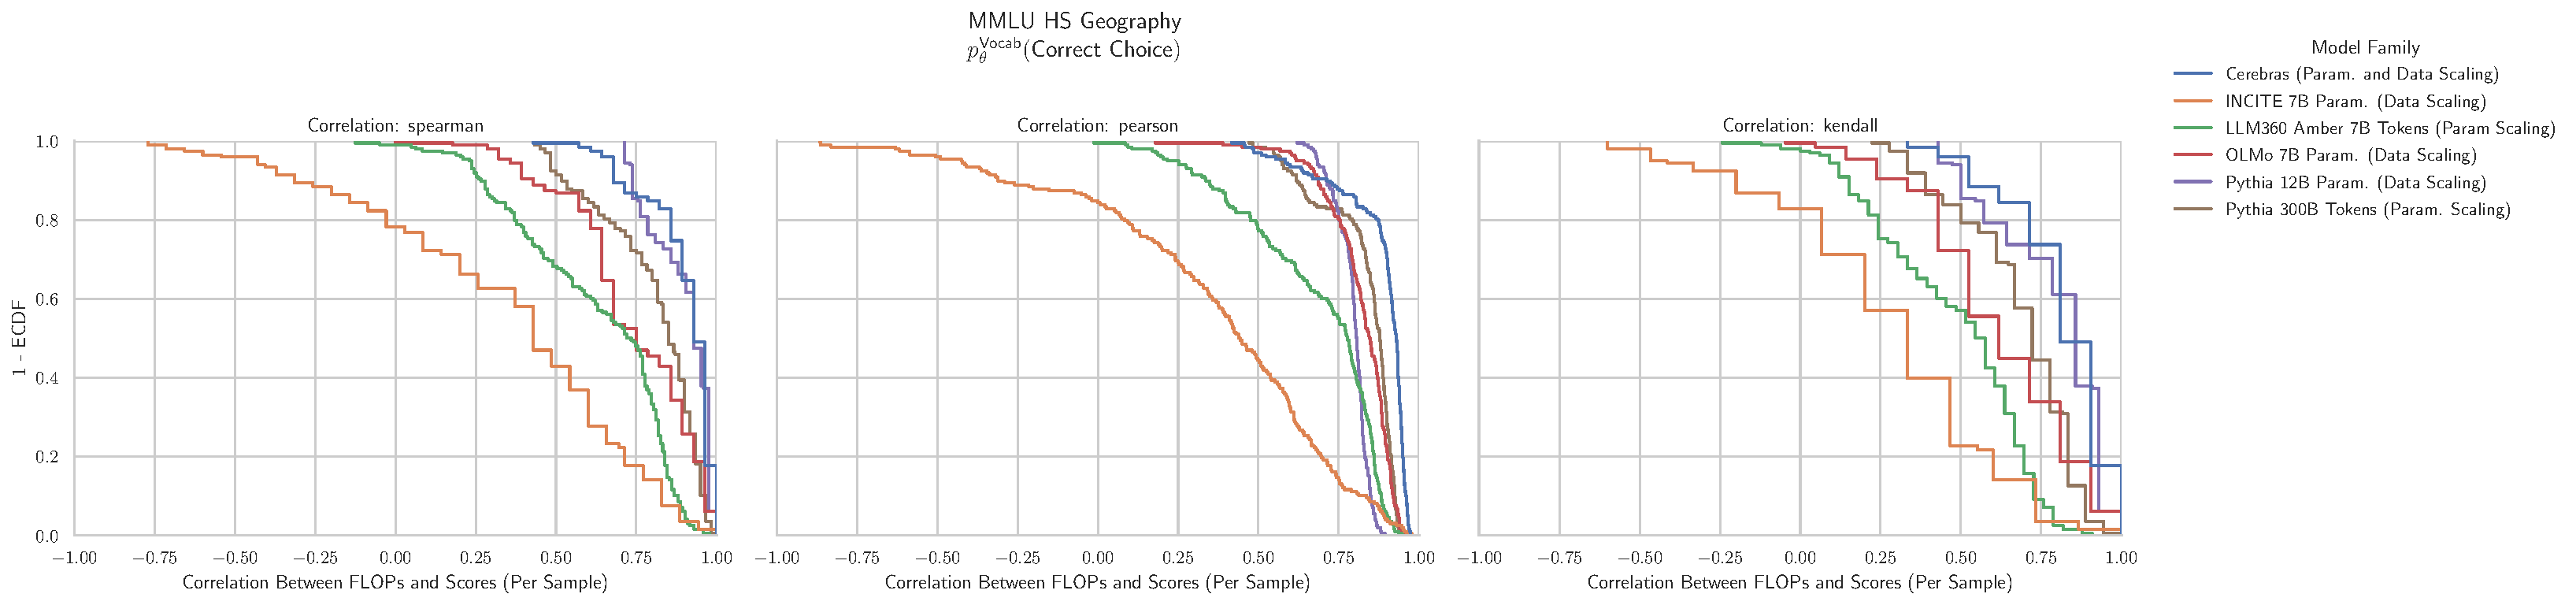
\includegraphics[width=\textwidth]{figures/correlations_between_scores_and_compute/correlation_distributions/mmlu_high_school_geography/mmlu_high_school_geography_prob_correct_vocab_ecdf_vs_correlation_score_by_modelfamily_split_correlation_metric.pdf}
    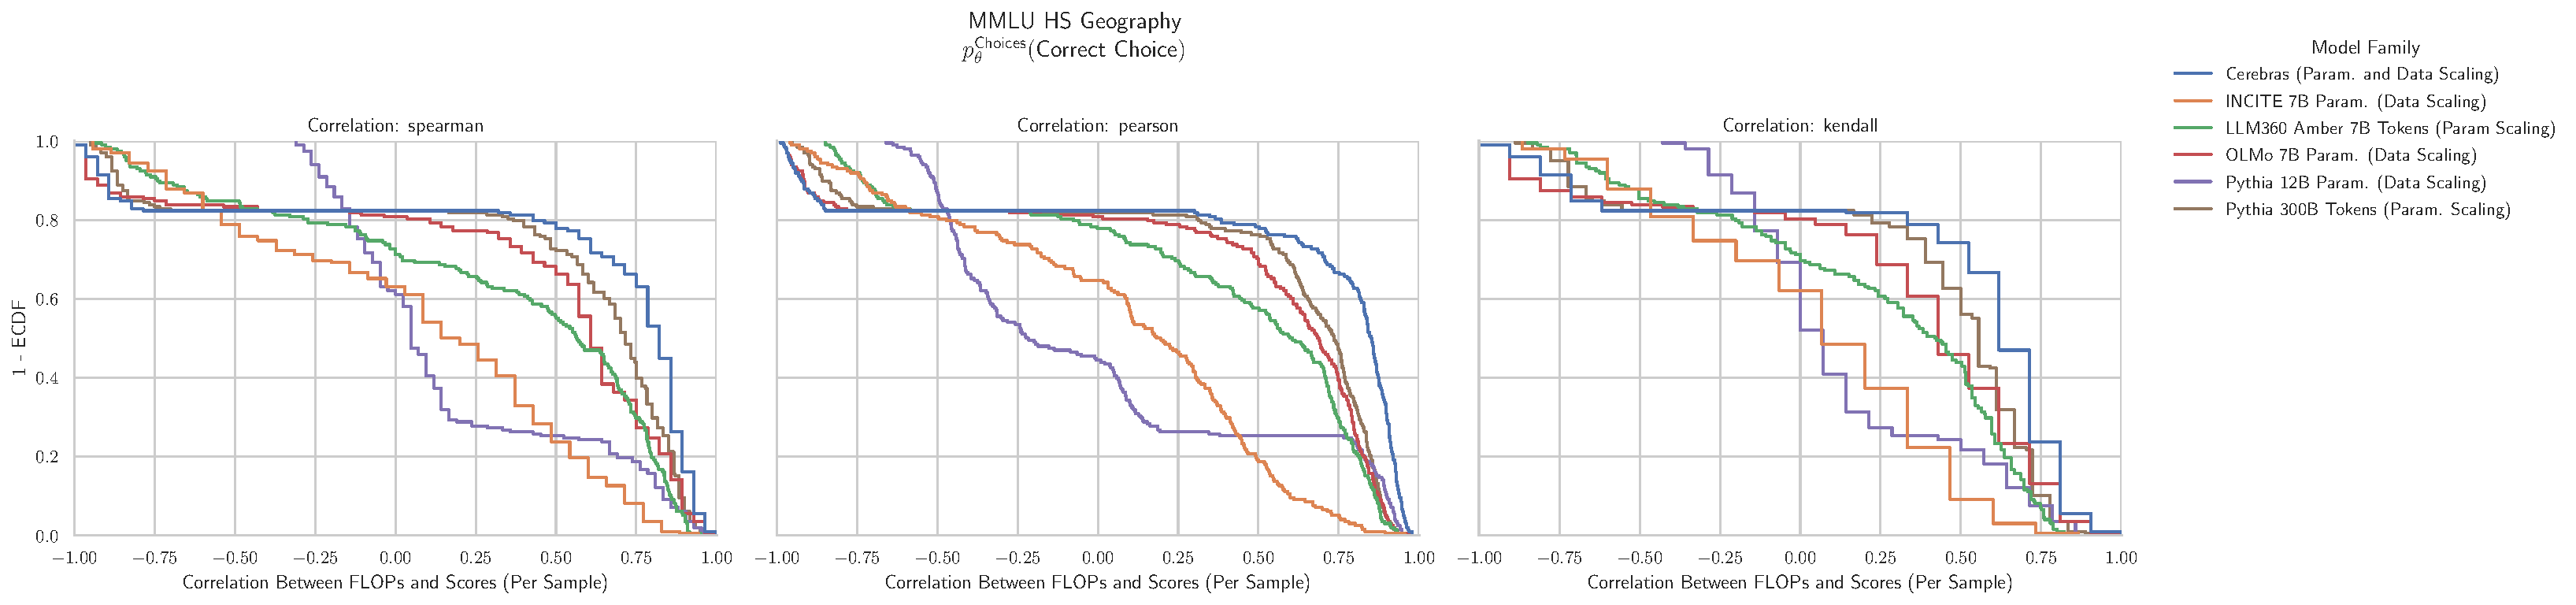
\includegraphics[width=\textwidth]{figures/correlations_between_scores_and_compute/correlation_distributions/mmlu_high_school_geography/mmlu_high_school_geography_prob_correct_choices_ecdf_vs_correlation_score_by_modelfamily_split_correlation_metric.pdf}
    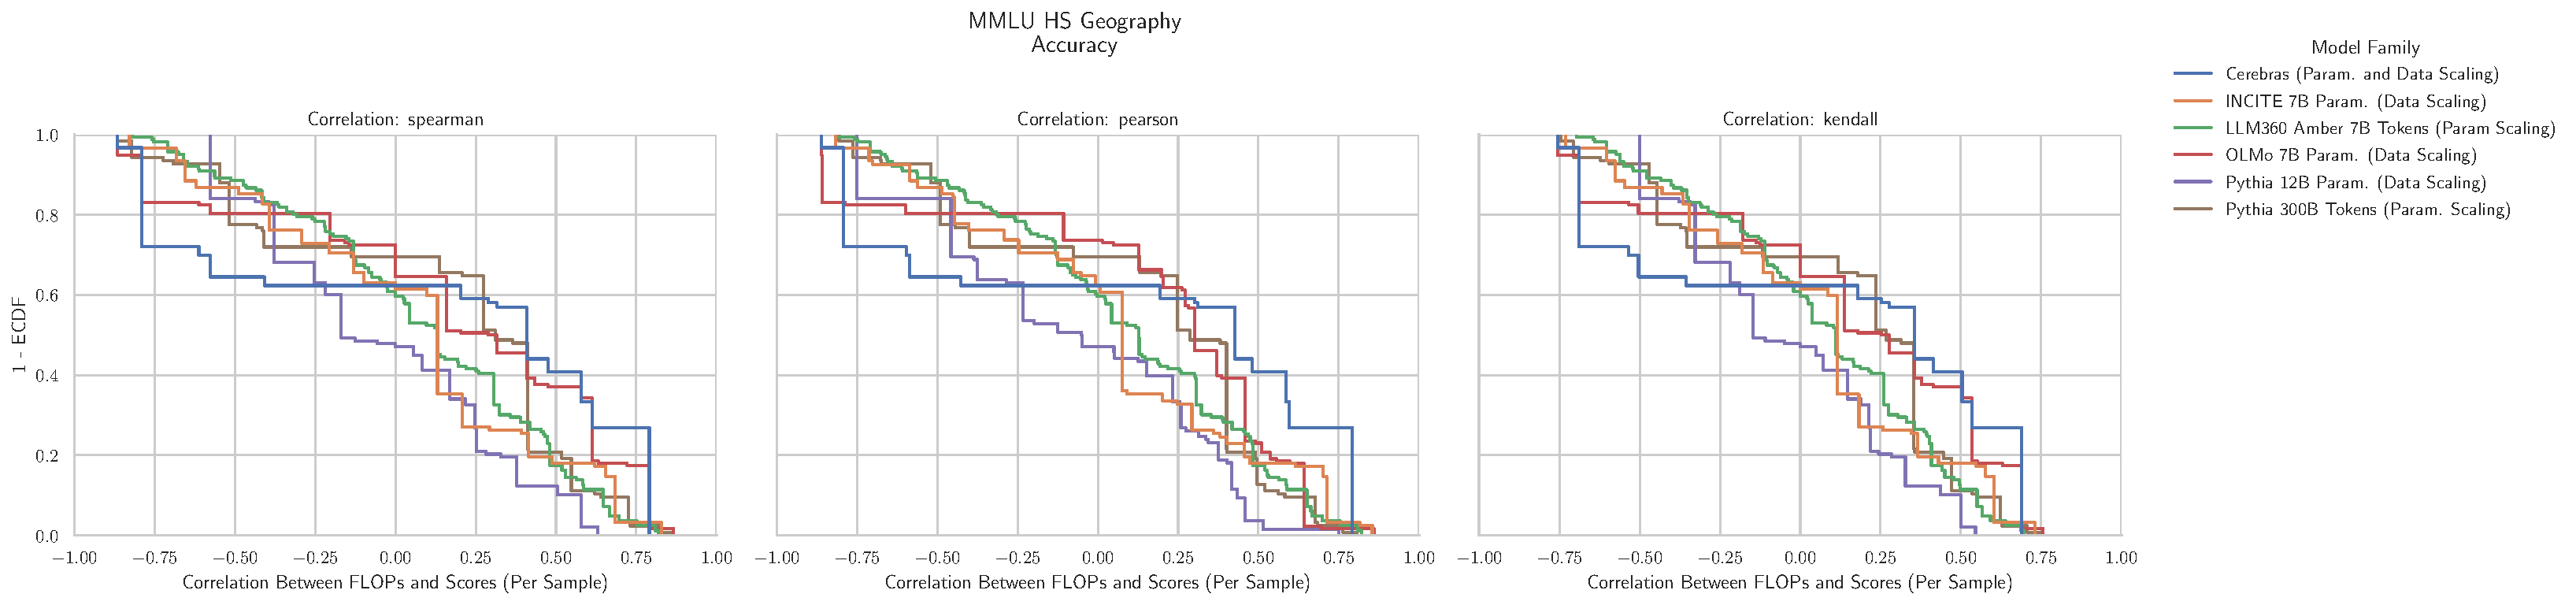
\includegraphics[width=\textwidth]{figures/correlations_between_scores_and_compute/correlation_distributions/mmlu_high_school_geography/mmlu_high_school_geography_acc_ecdf_vs_correlation_score_by_modelfamily_split_correlation_metric.pdf}
    \caption{\textbf{MMLU High School Geography: Downstream performance is computed via a sequence of transformations that deteriorate correlations between scores and pretraining compute.}}
    \label{app:fig:compute_score_distribution_mmlu_high_school_geography}
\end{figure}


\clearpage
\subsection{NLP Benchmark: MMLU High School Government \& Politics \cite{hendrycks2020mmlu}}

\begin{figure}[h!]
    \centering
    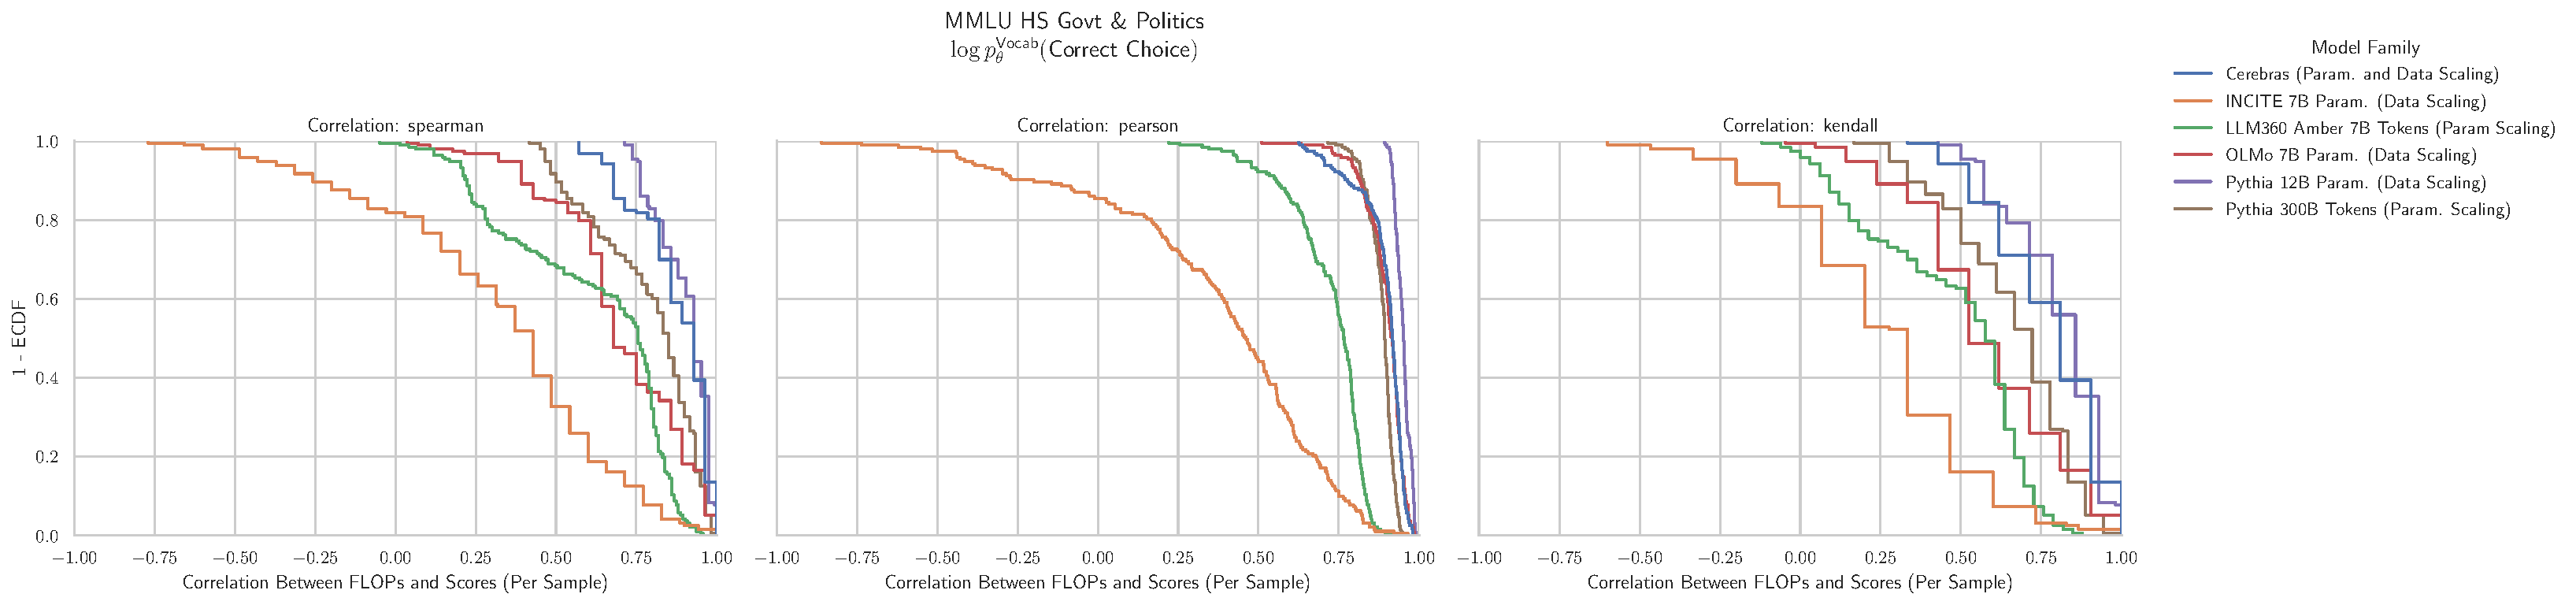
\includegraphics[width=\textwidth]{figures/correlations_between_scores_and_compute/correlation_distributions/mmlu_high_school_government_and_politics/mmlu_high_school_government_and_politics_log_likelihood_correct_ecdf_vs_correlation_score_by_modelfamily_split_correlation_metric.pdf}
    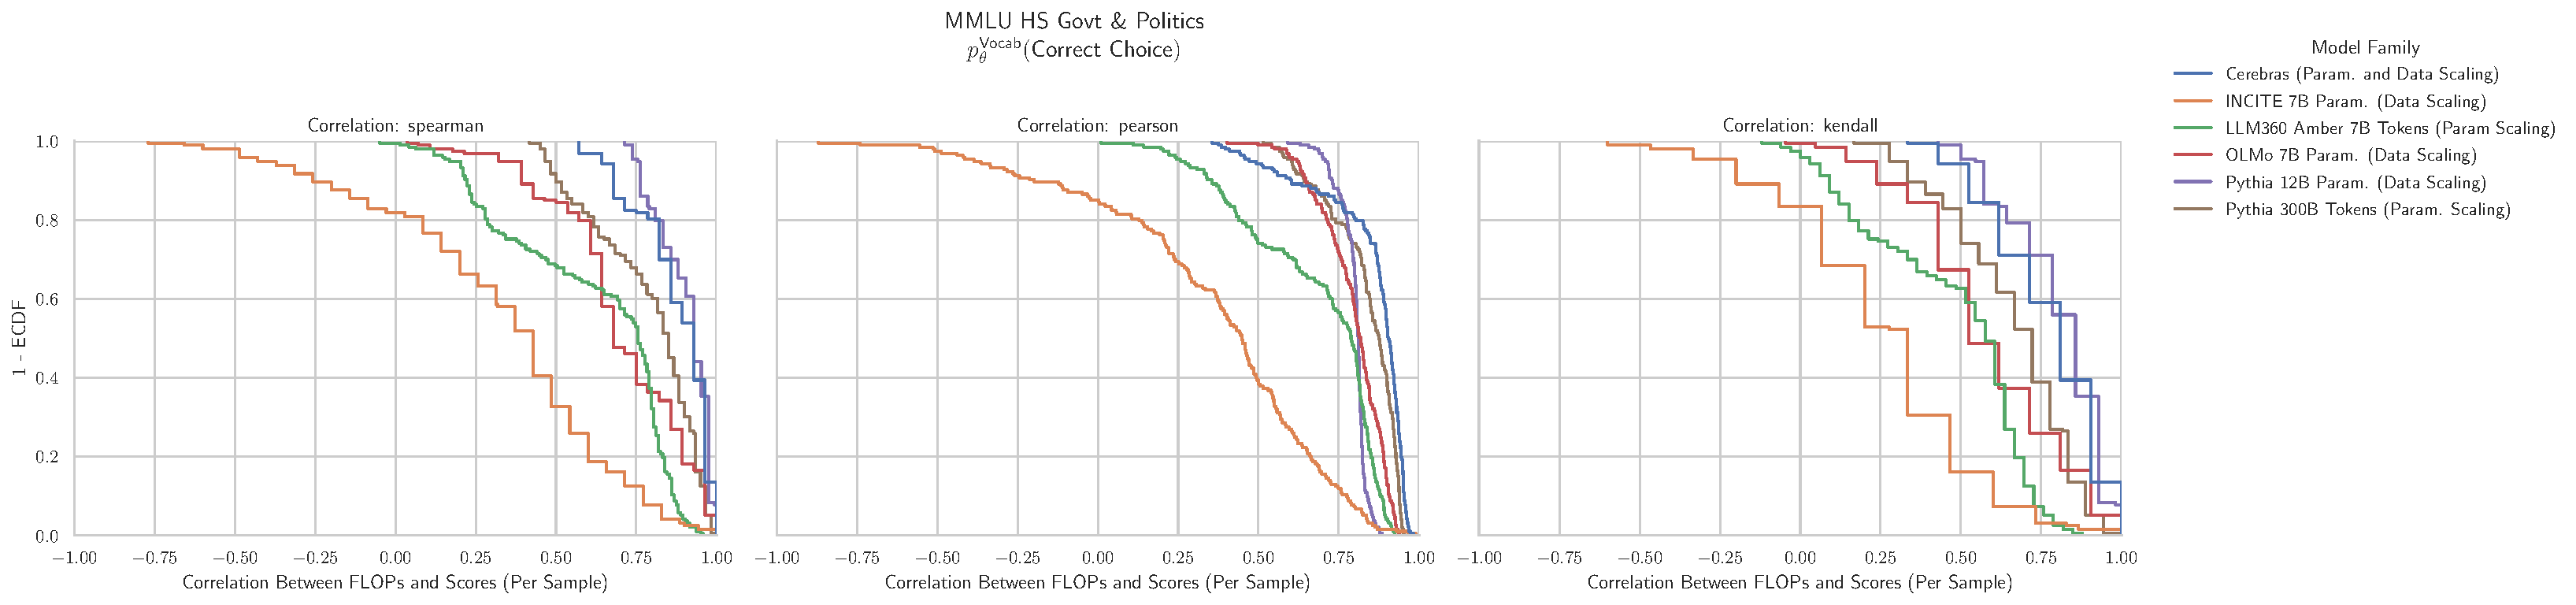
\includegraphics[width=\textwidth]{figures/correlations_between_scores_and_compute/correlation_distributions/mmlu_high_school_government_and_politics/mmlu_high_school_government_and_politics_prob_correct_vocab_ecdf_vs_correlation_score_by_modelfamily_split_correlation_metric.pdf}
    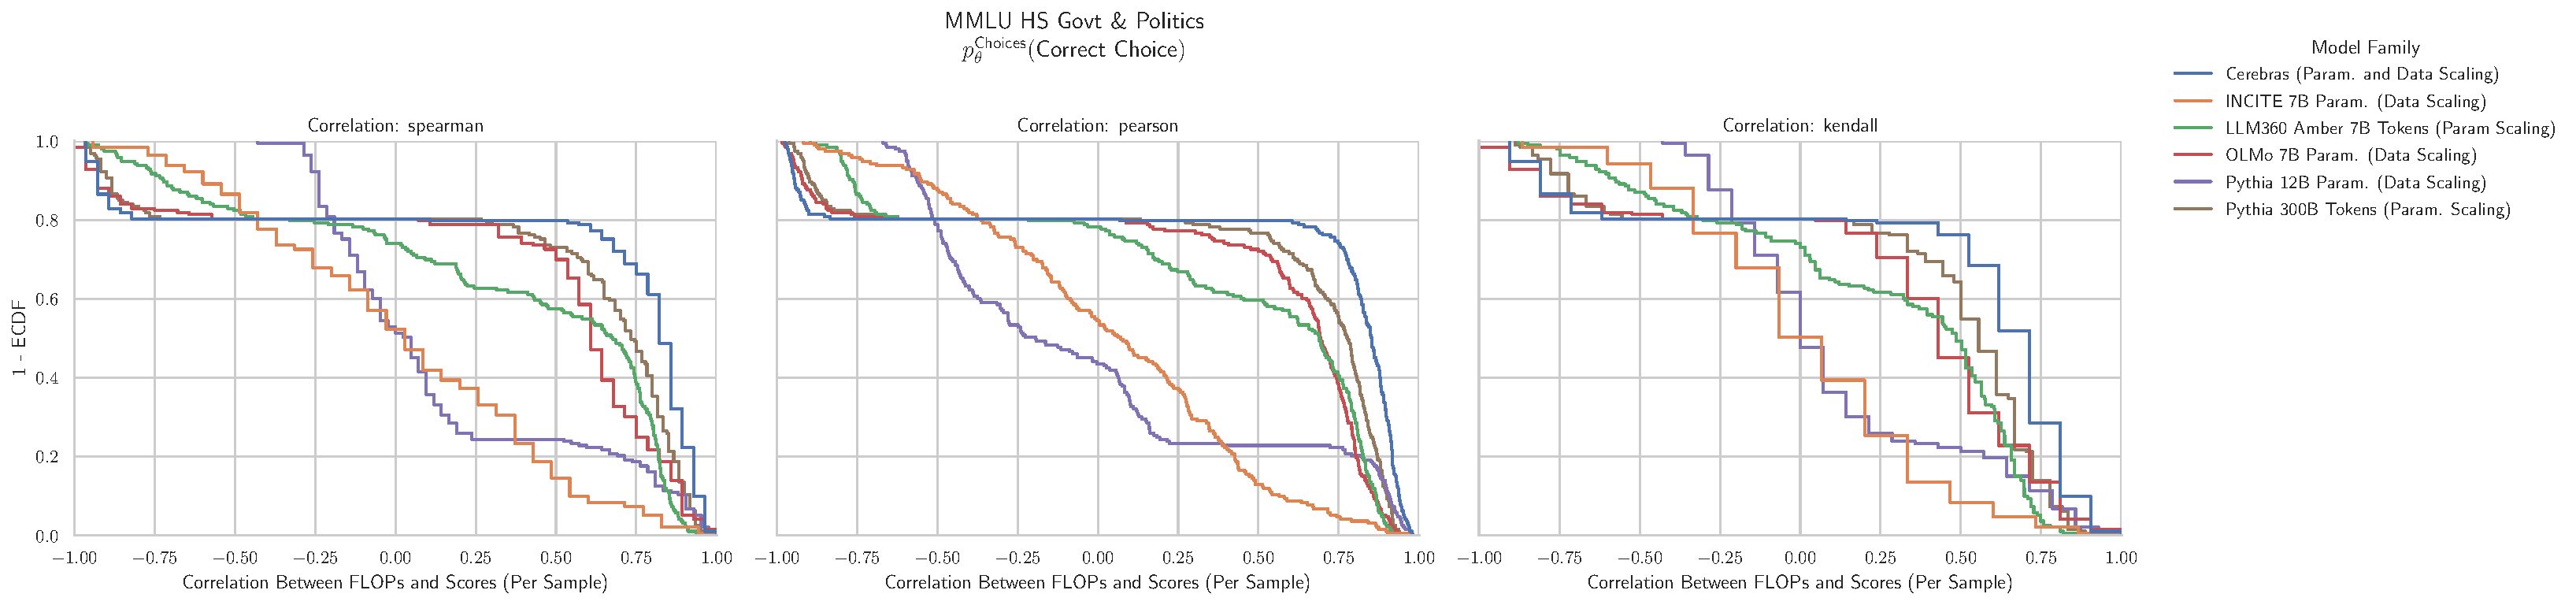
\includegraphics[width=\textwidth]{figures/correlations_between_scores_and_compute/correlation_distributions/mmlu_high_school_government_and_politics/mmlu_high_school_government_and_politics_prob_correct_choices_ecdf_vs_correlation_score_by_modelfamily_split_correlation_metric.pdf}
    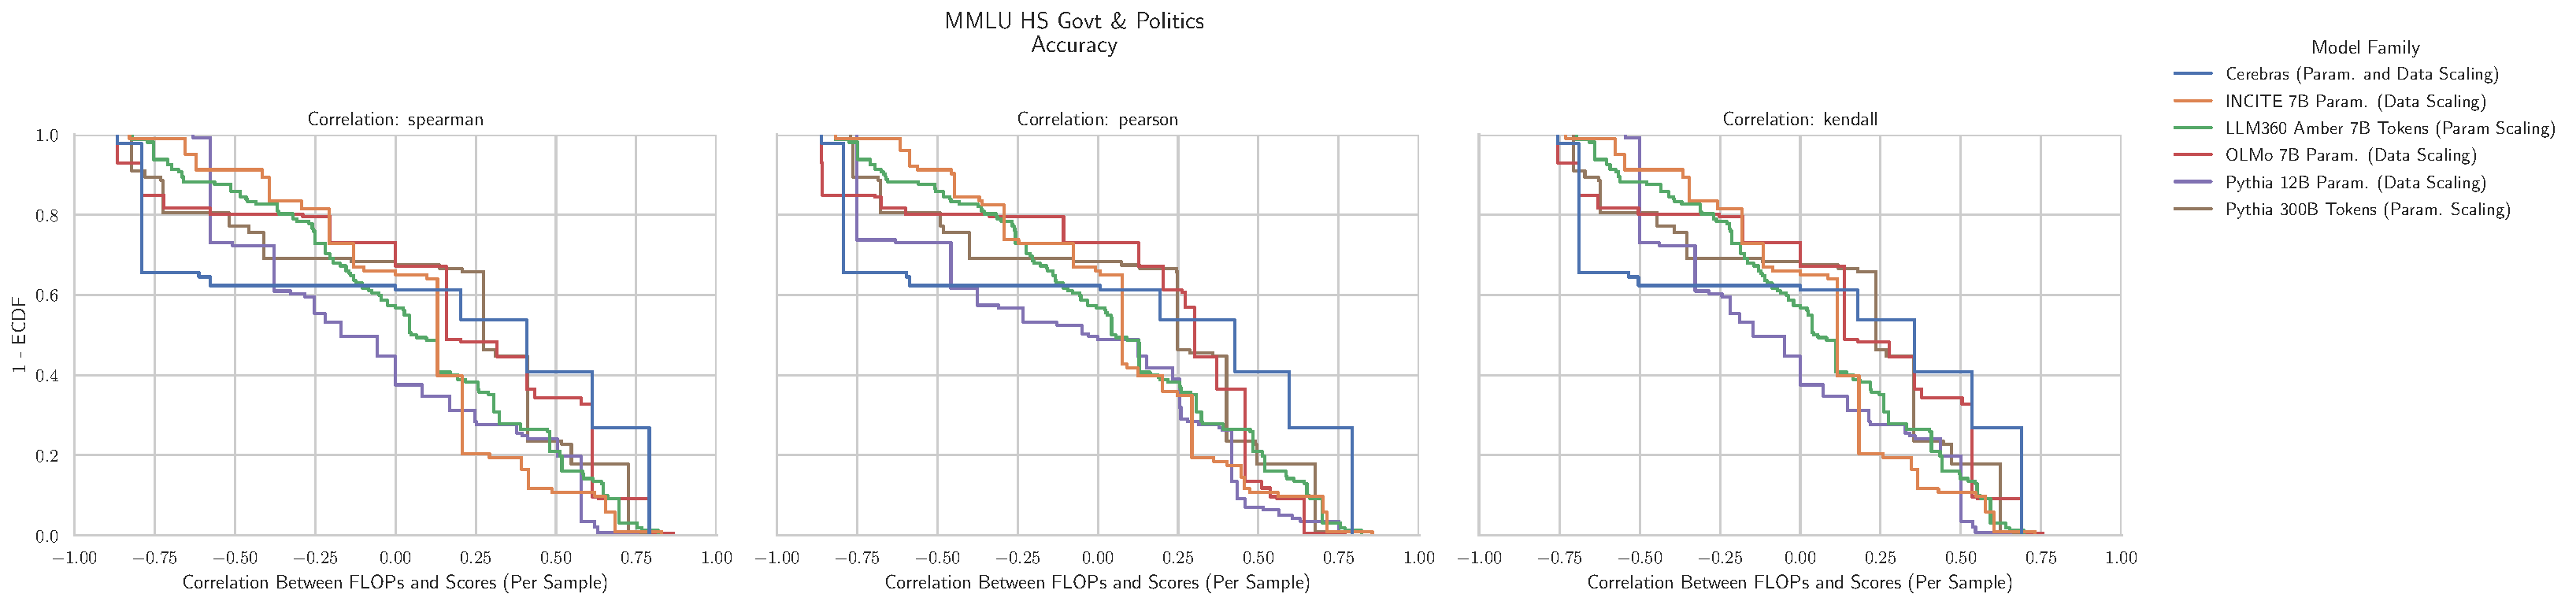
\includegraphics[width=\textwidth]{figures/correlations_between_scores_and_compute/correlation_distributions/mmlu_high_school_government_and_politics/mmlu_high_school_government_and_politics_acc_ecdf_vs_correlation_score_by_modelfamily_split_correlation_metric.pdf}
    \caption{\textbf{MMLU High School Government \& Politics: Downstream performance is computed via a sequence of transformations that deteriorate correlations between scores and pretraining compute.}}
    \label{app:fig:compute_score_distribution_mmlu_high_school_government_and_politics}
\end{figure}


\clearpage
\subsection{NLP Benchmark: MMLU High School Macroeconomics \cite{hendrycks2020mmlu}}

\begin{figure}[h!]
    \centering
    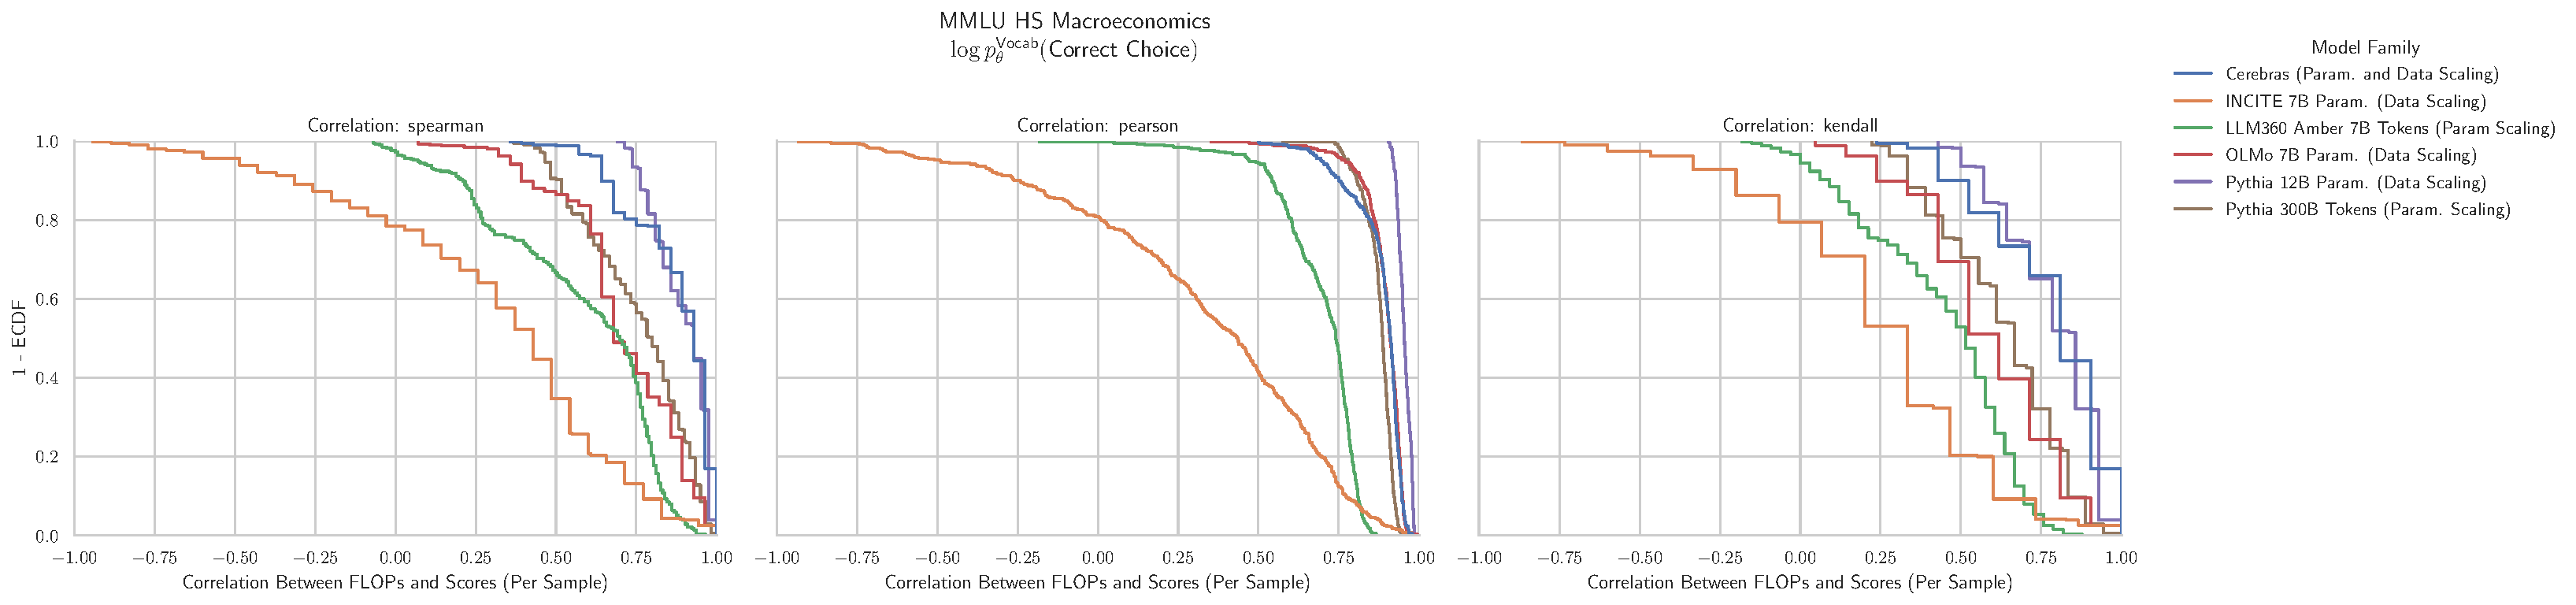
\includegraphics[width=\textwidth]{figures/correlations_between_scores_and_compute/correlation_distributions/mmlu_high_school_macroeconomics/mmlu_high_school_macroeconomics_log_likelihood_correct_ecdf_vs_correlation_score_by_modelfamily_split_correlation_metric.pdf}
    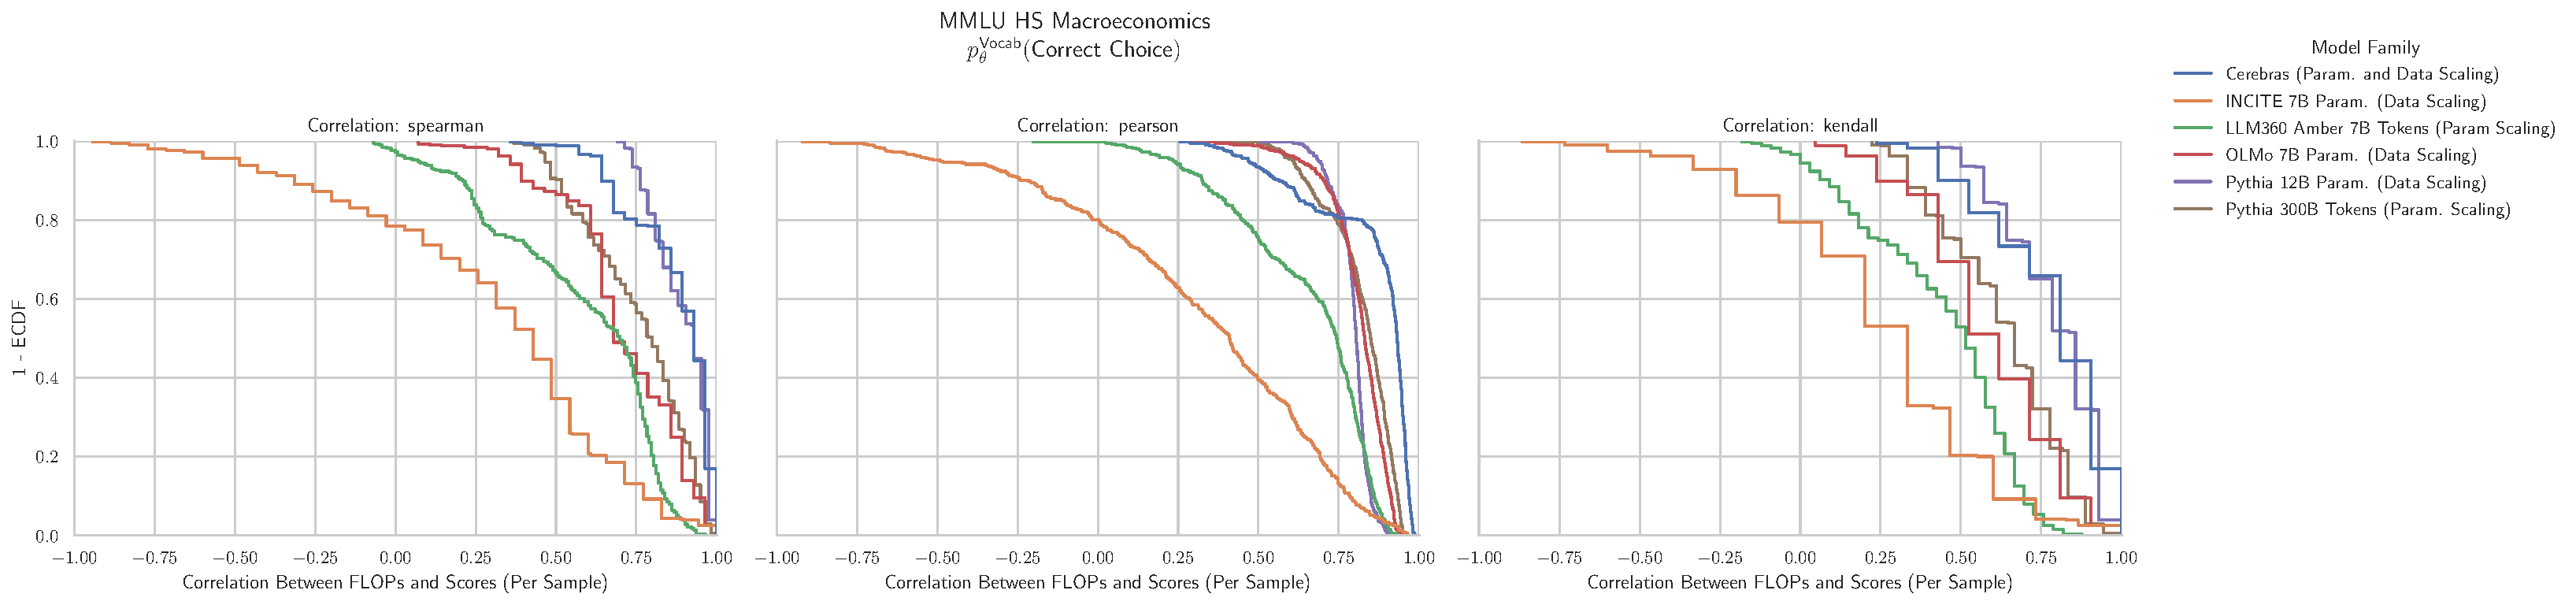
\includegraphics[width=\textwidth]{figures/correlations_between_scores_and_compute/correlation_distributions/mmlu_high_school_macroeconomics/mmlu_high_school_macroeconomics_prob_correct_vocab_ecdf_vs_correlation_score_by_modelfamily_split_correlation_metric.pdf}
    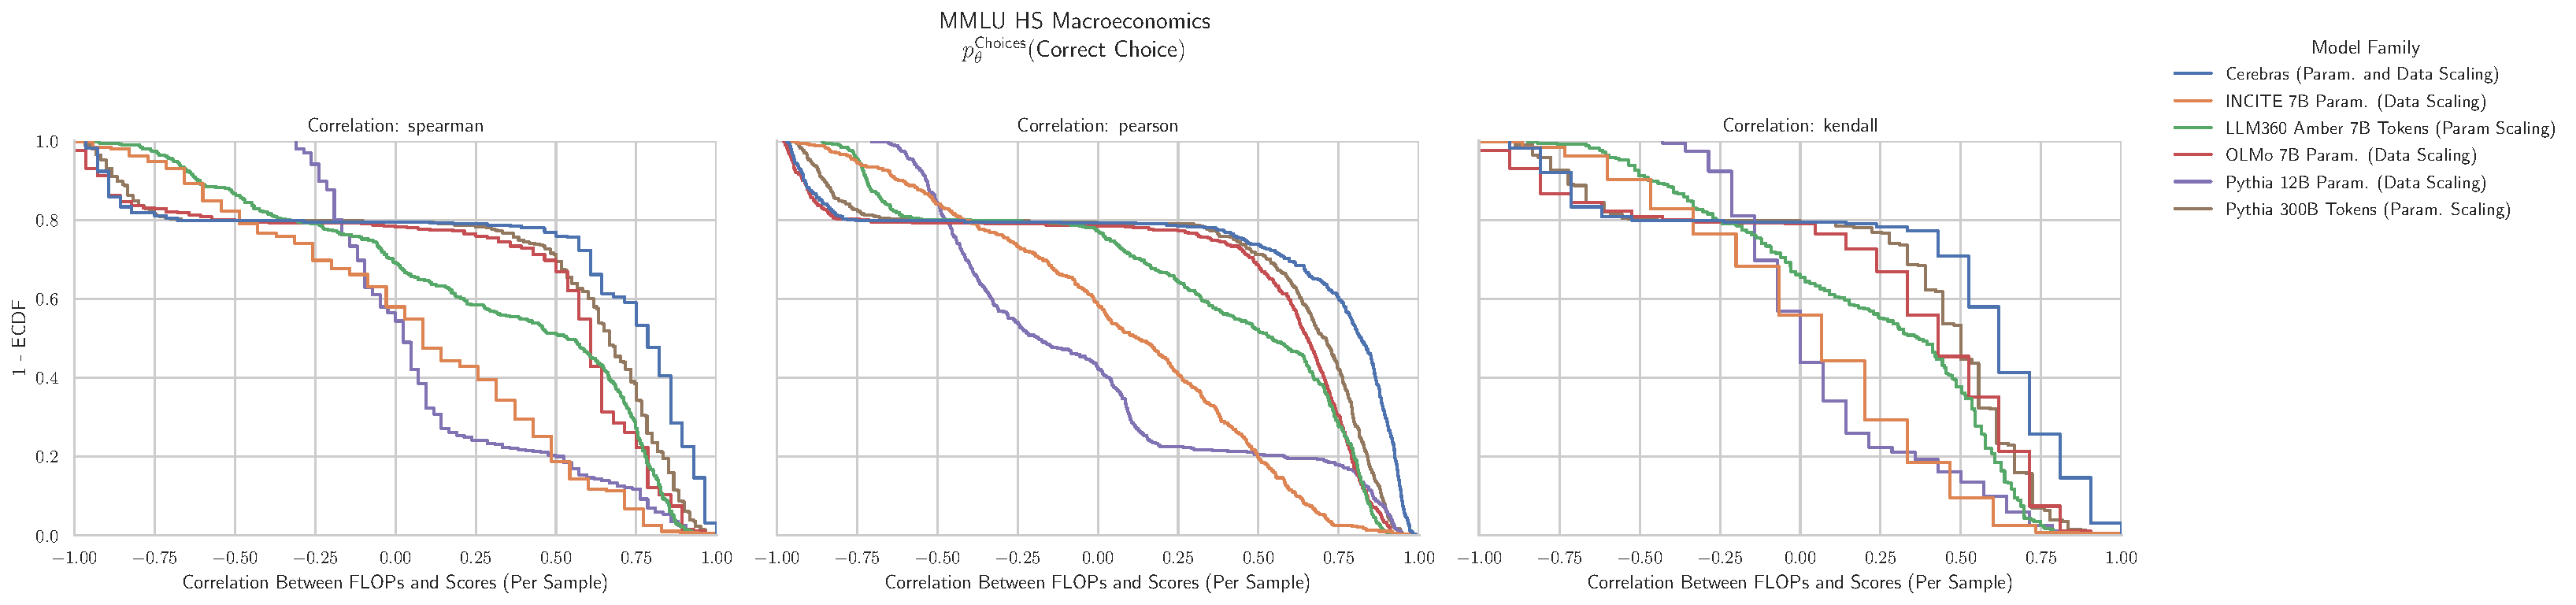
\includegraphics[width=\textwidth]{figures/correlations_between_scores_and_compute/correlation_distributions/mmlu_high_school_macroeconomics/mmlu_high_school_macroeconomics_prob_correct_choices_ecdf_vs_correlation_score_by_modelfamily_split_correlation_metric.pdf}
    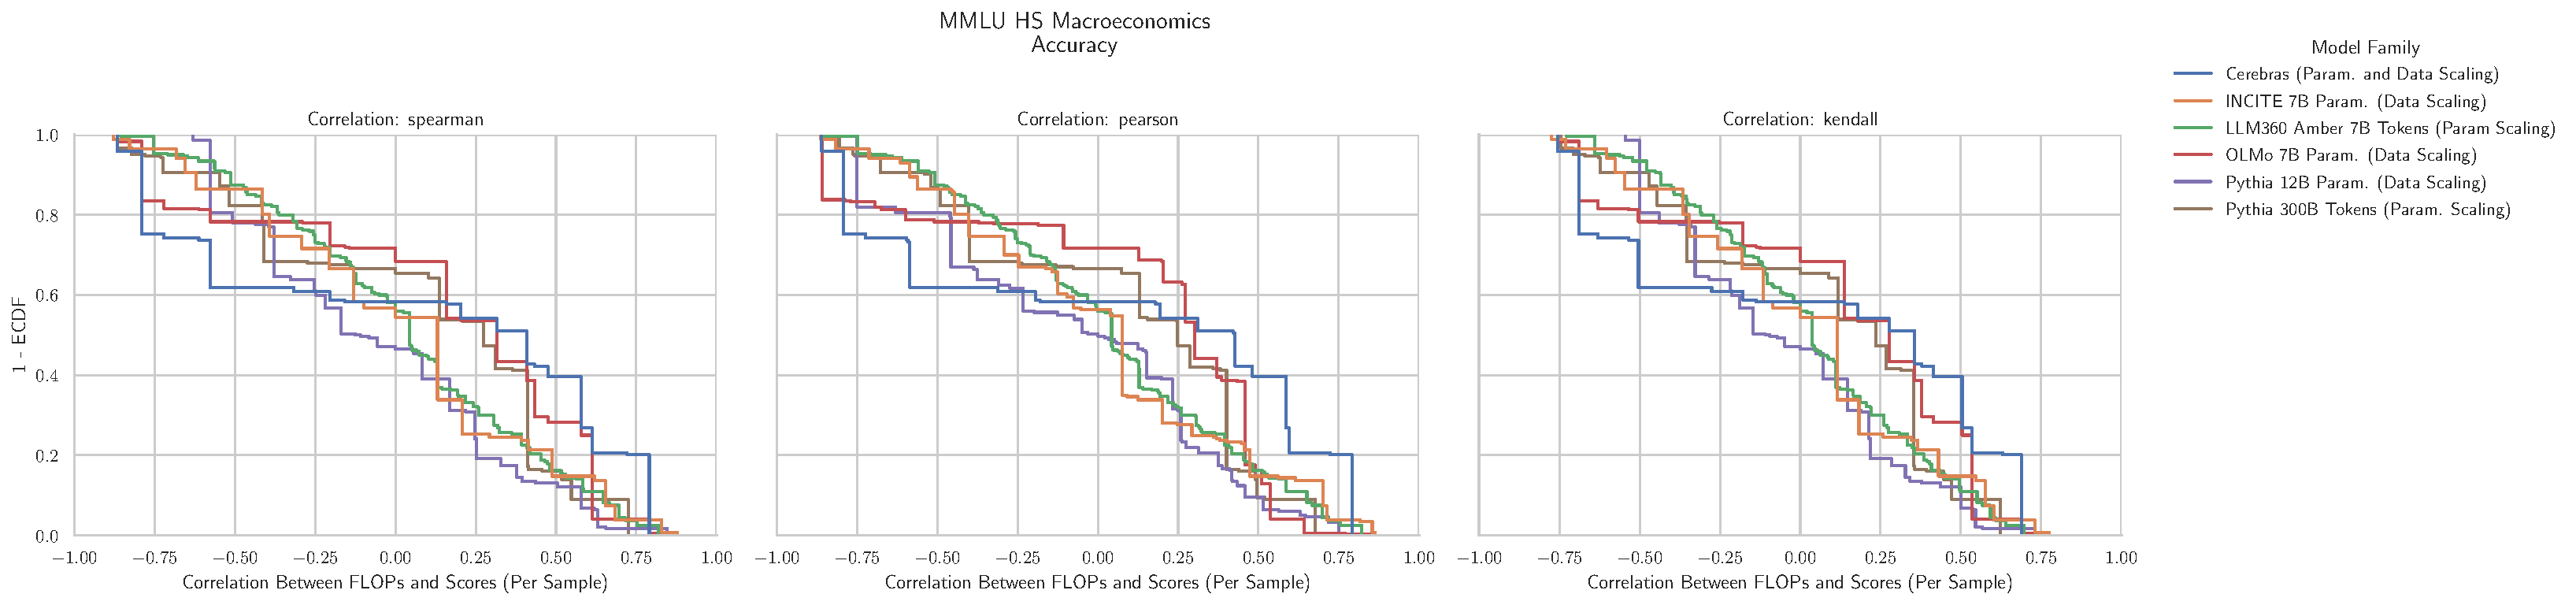
\includegraphics[width=\textwidth]{figures/correlations_between_scores_and_compute/correlation_distributions/mmlu_high_school_macroeconomics/mmlu_high_school_macroeconomics_acc_ecdf_vs_correlation_score_by_modelfamily_split_correlation_metric.pdf}
    \caption{\textbf{MMLU High School Macroeconomics: Downstream performance is computed via a sequence of transformations that deteriorate correlations between scores and pretraining compute.}}
    \label{app:fig:compute_score_distribution_mmlu_high_school_macroeconomics}
\end{figure}


\clearpage
\subsection{NLP Benchmark: MMLU High School Mathematics \cite{hendrycks2020mmlu}}

\begin{figure}[h!]
    \centering
    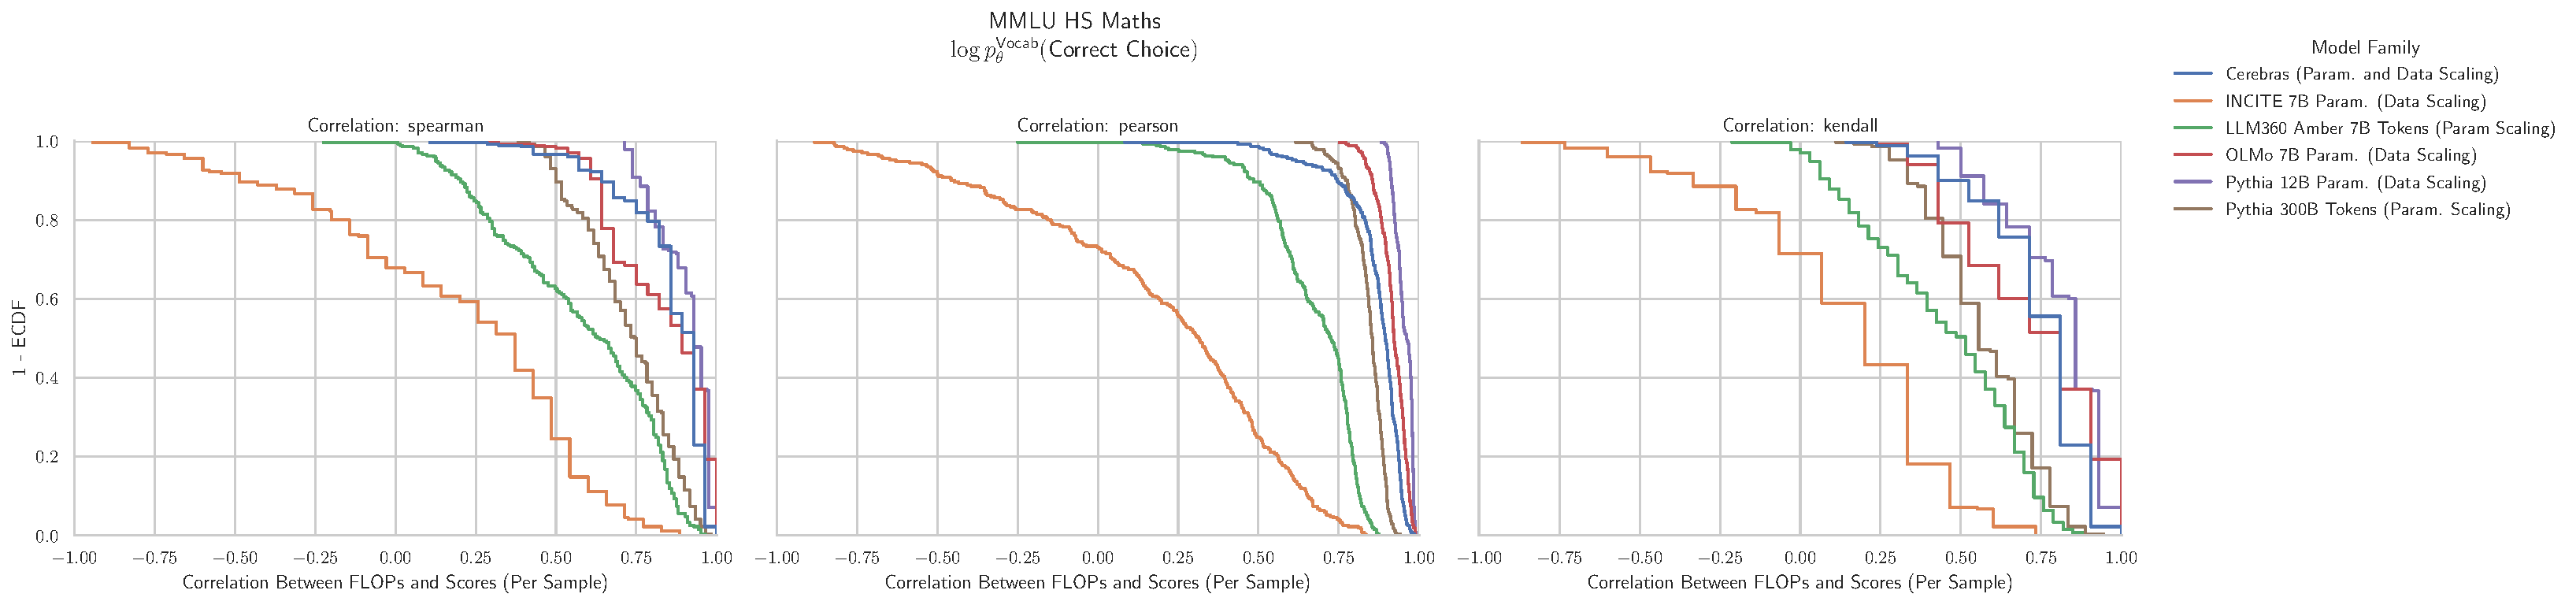
\includegraphics[width=\textwidth]{figures/correlations_between_scores_and_compute/correlation_distributions/mmlu_high_school_mathematics/mmlu_high_school_mathematics_log_likelihood_correct_ecdf_vs_correlation_score_by_modelfamily_split_correlation_metric.pdf}
    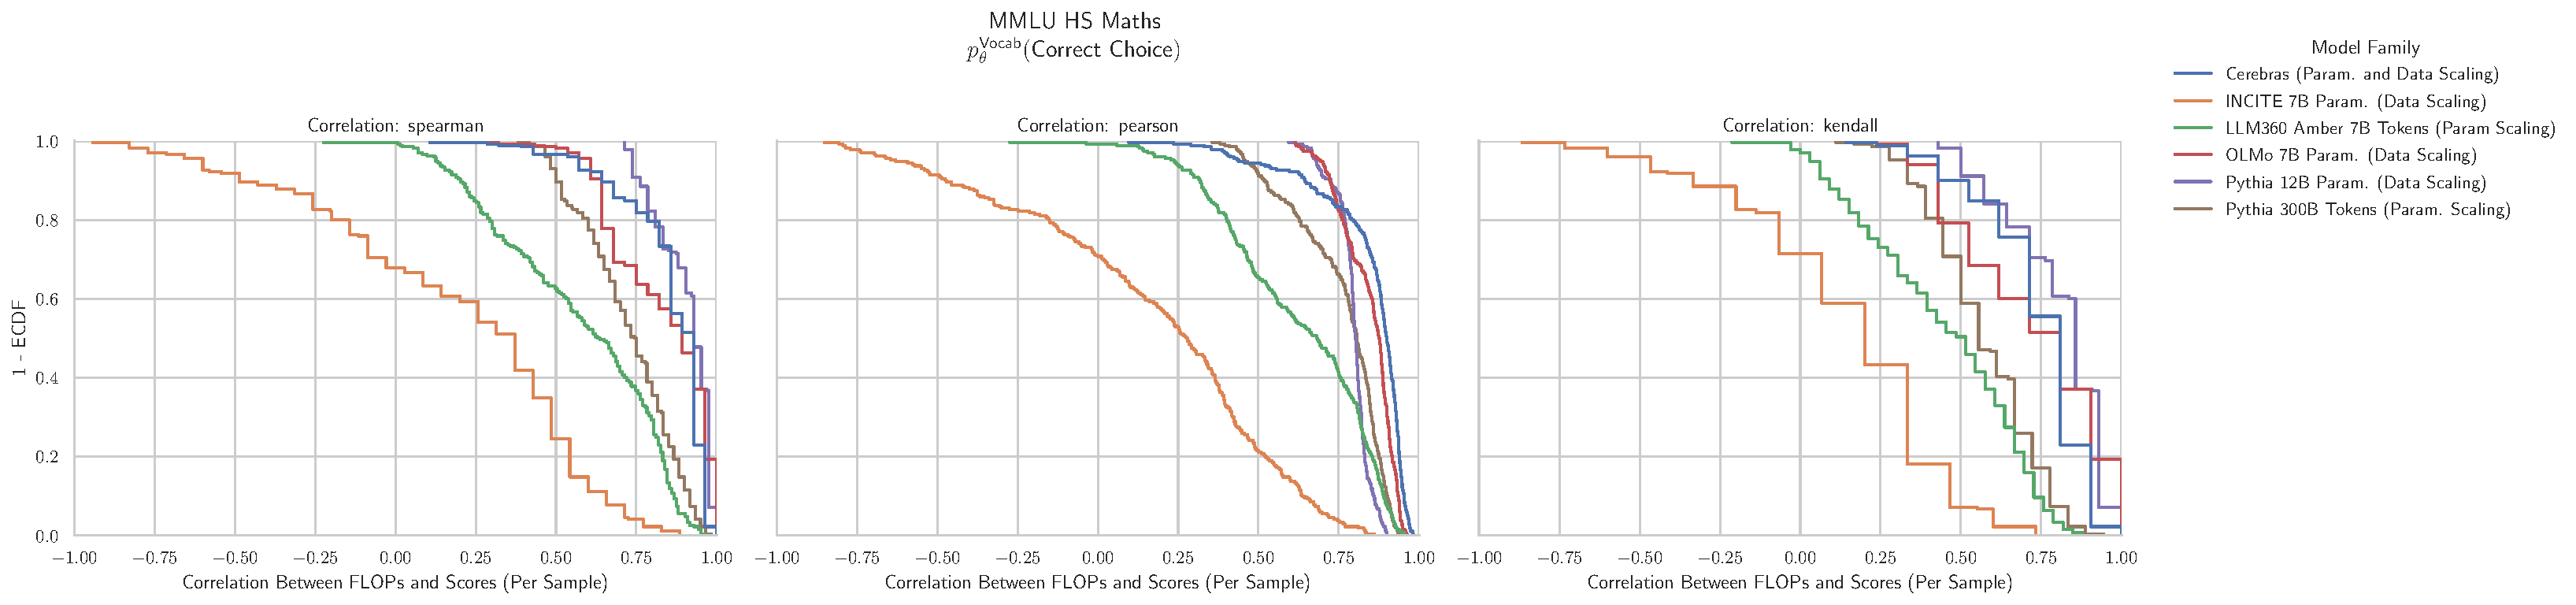
\includegraphics[width=\textwidth]{figures/correlations_between_scores_and_compute/correlation_distributions/mmlu_high_school_mathematics/mmlu_high_school_mathematics_prob_correct_vocab_ecdf_vs_correlation_score_by_modelfamily_split_correlation_metric.pdf}
    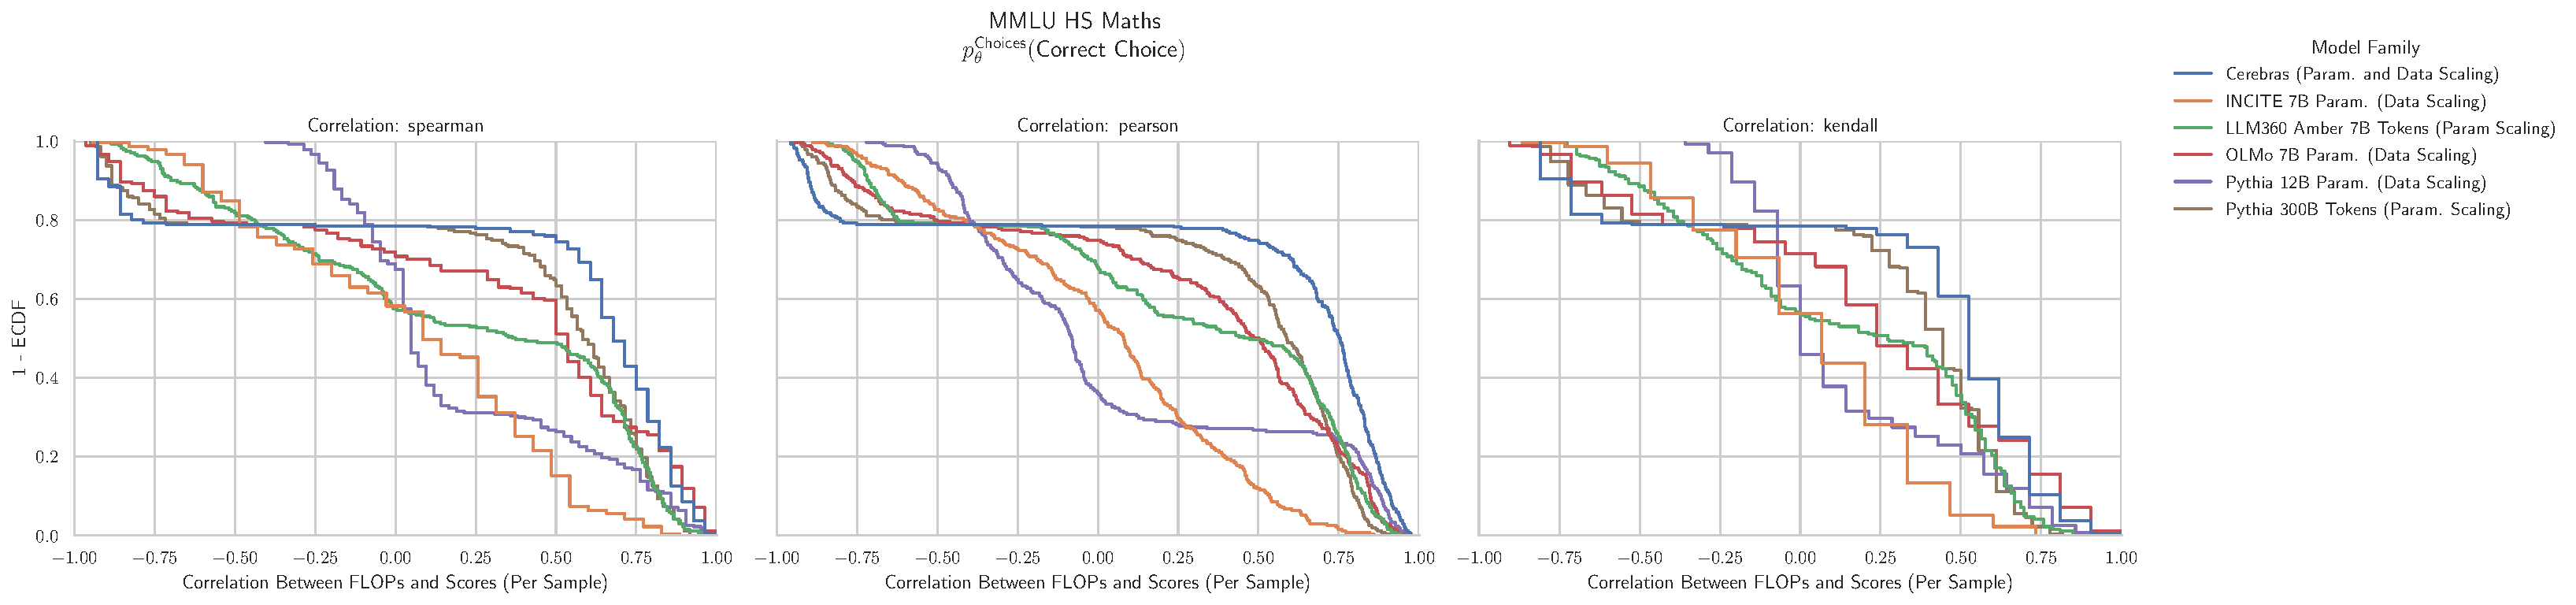
\includegraphics[width=\textwidth]{figures/correlations_between_scores_and_compute/correlation_distributions/mmlu_high_school_mathematics/mmlu_high_school_mathematics_prob_correct_choices_ecdf_vs_correlation_score_by_modelfamily_split_correlation_metric.pdf}
    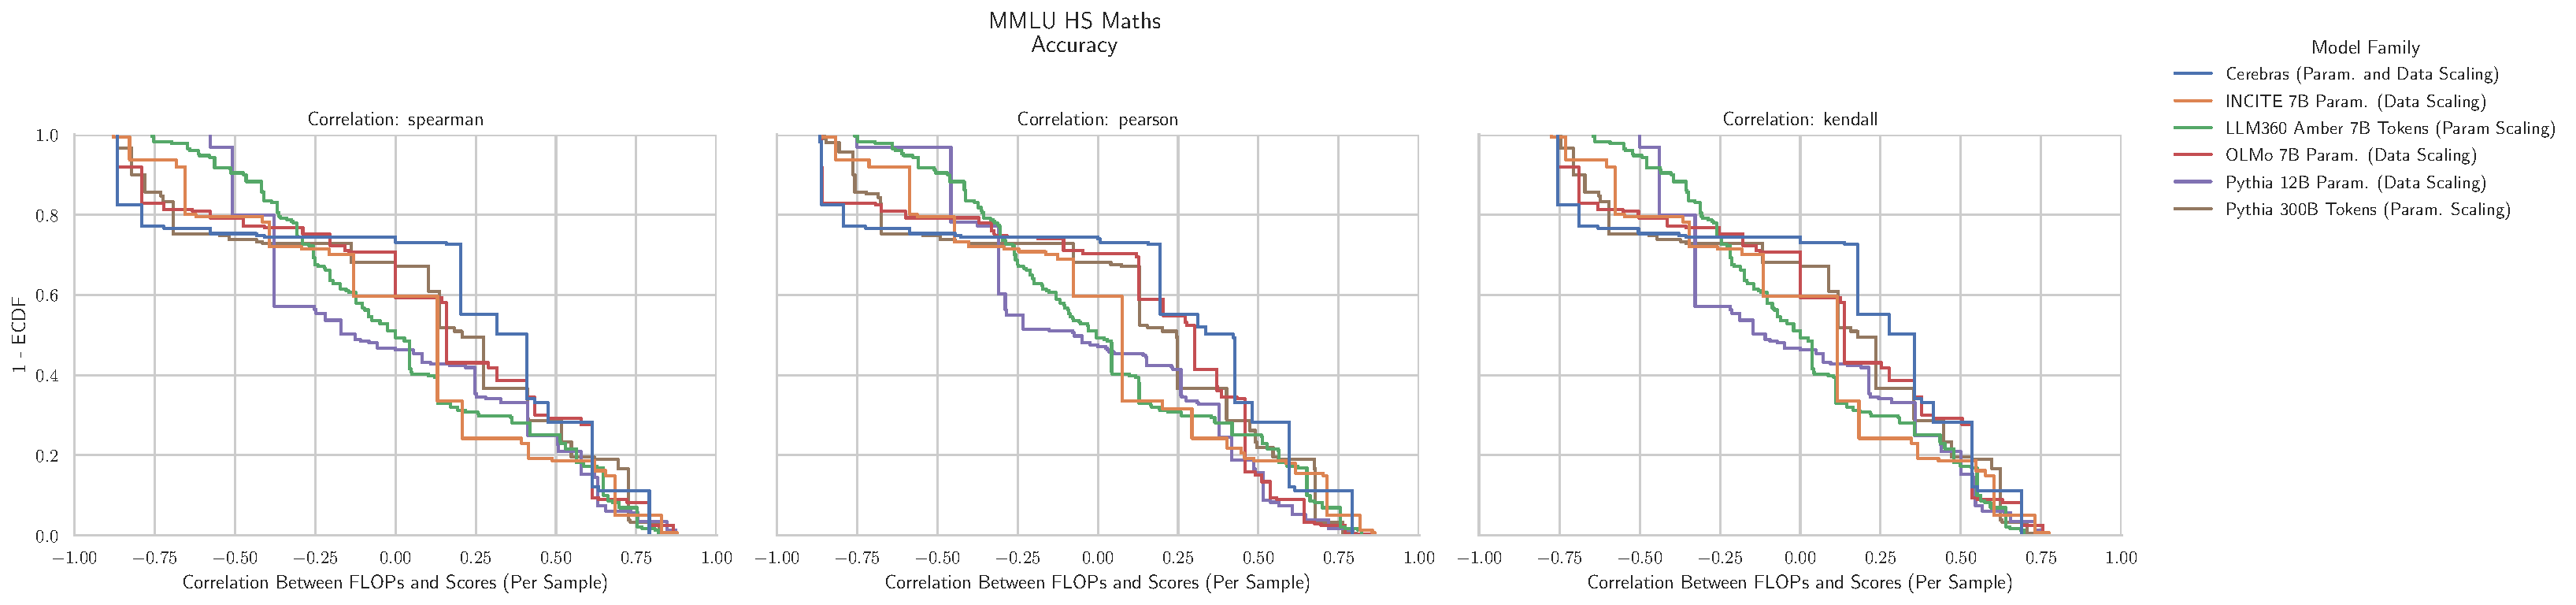
\includegraphics[width=\textwidth]{figures/correlations_between_scores_and_compute/correlation_distributions/mmlu_high_school_mathematics/mmlu_high_school_mathematics_acc_ecdf_vs_correlation_score_by_modelfamily_split_correlation_metric.pdf}
    \caption{\textbf{MMLU High School Mathematics: Downstream performance is computed via a sequence of transformations that deteriorate correlations between scores and pretraining compute.}}
    \label{app:fig:compute_score_distribution_mmlu_high_school_mathematics}
\end{figure}



\clearpage
\subsection{NLP Benchmark: MMLU High School Microeconomics \cite{hendrycks2020mmlu}}

\begin{figure}[h!]
    \centering
    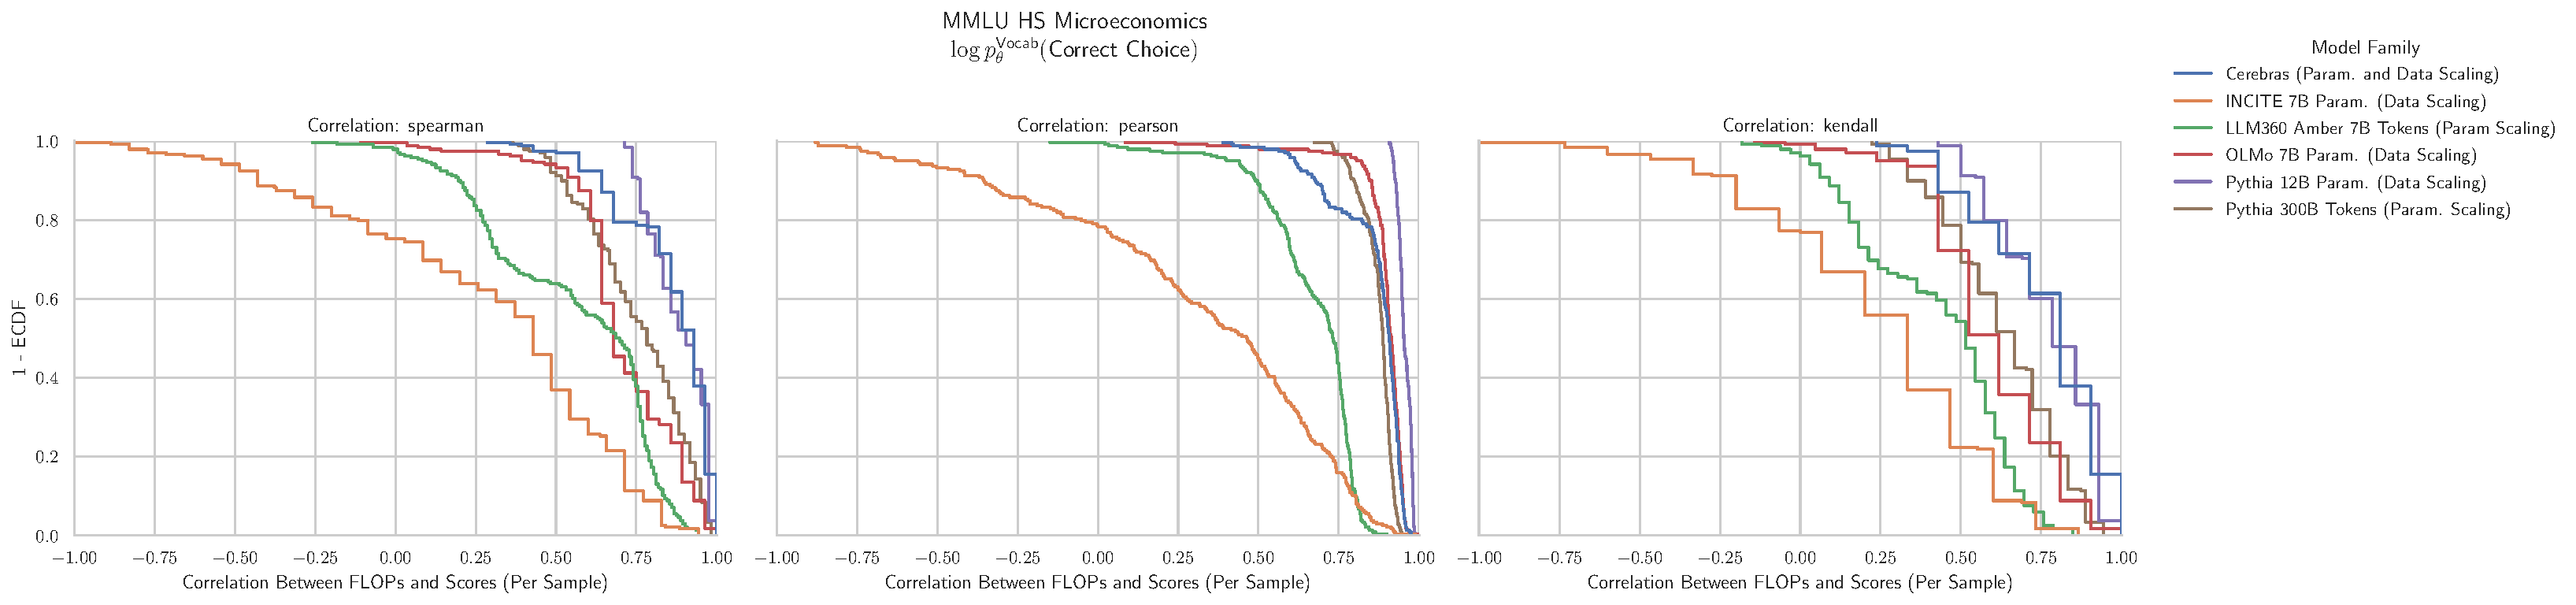
\includegraphics[width=\textwidth]{figures/correlations_between_scores_and_compute/correlation_distributions/mmlu_high_school_microeconomics/mmlu_high_school_microeconomics_log_likelihood_correct_ecdf_vs_correlation_score_by_modelfamily_split_correlation_metric.pdf}
    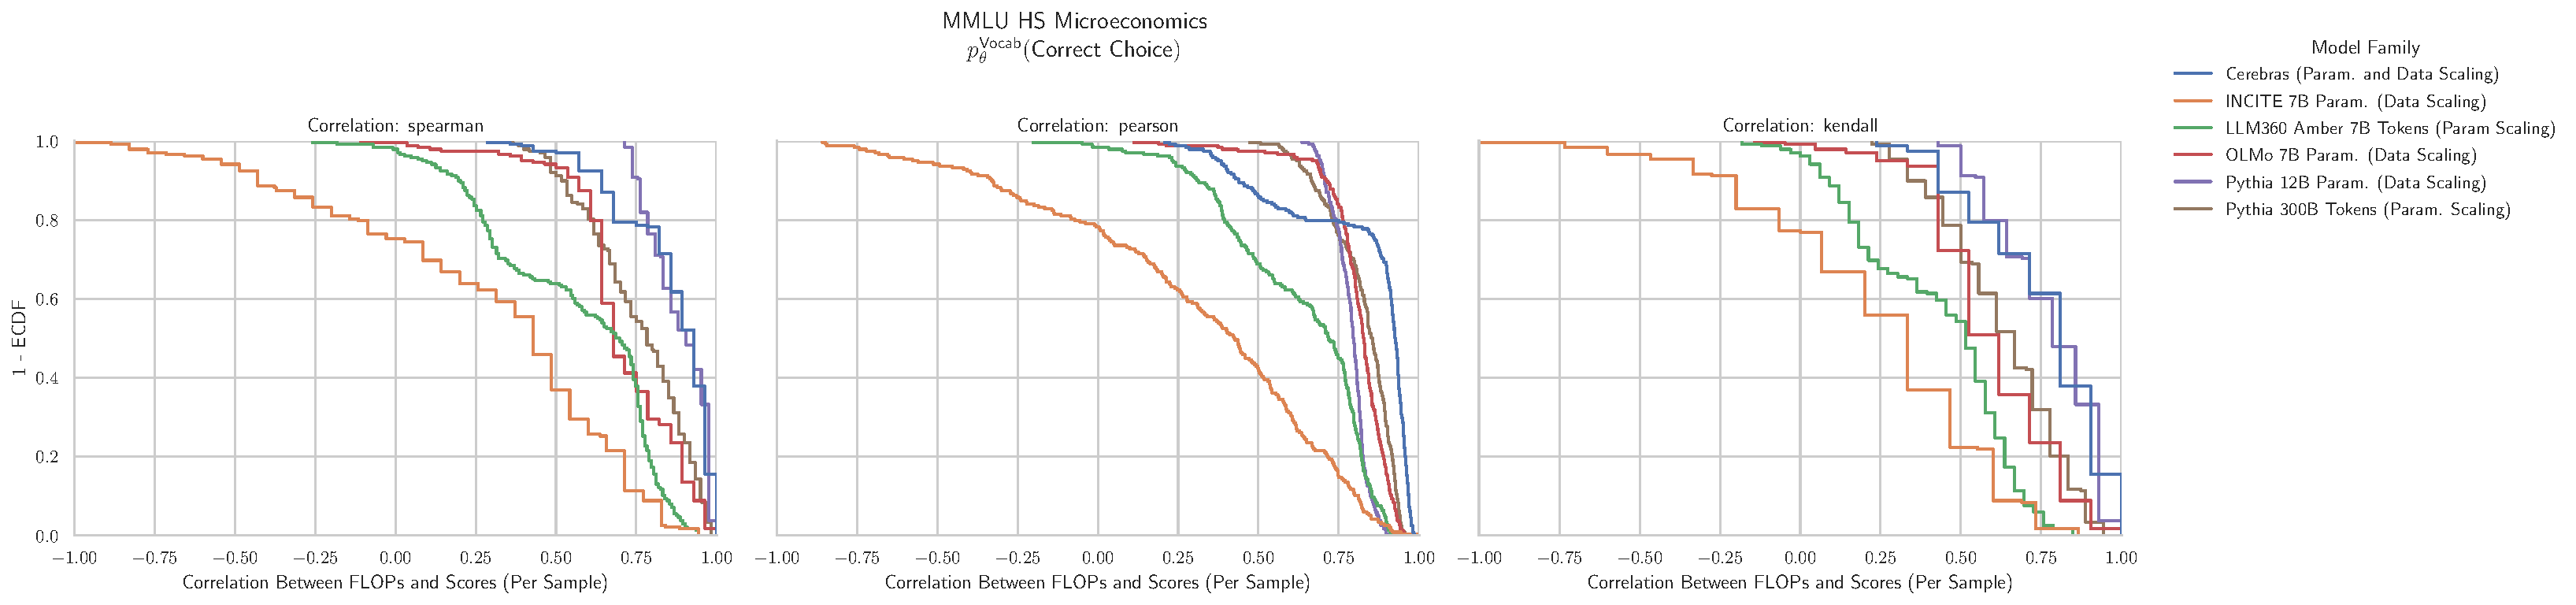
\includegraphics[width=\textwidth]{figures/correlations_between_scores_and_compute/correlation_distributions/mmlu_high_school_microeconomics/mmlu_high_school_microeconomics_prob_correct_vocab_ecdf_vs_correlation_score_by_modelfamily_split_correlation_metric.pdf}
    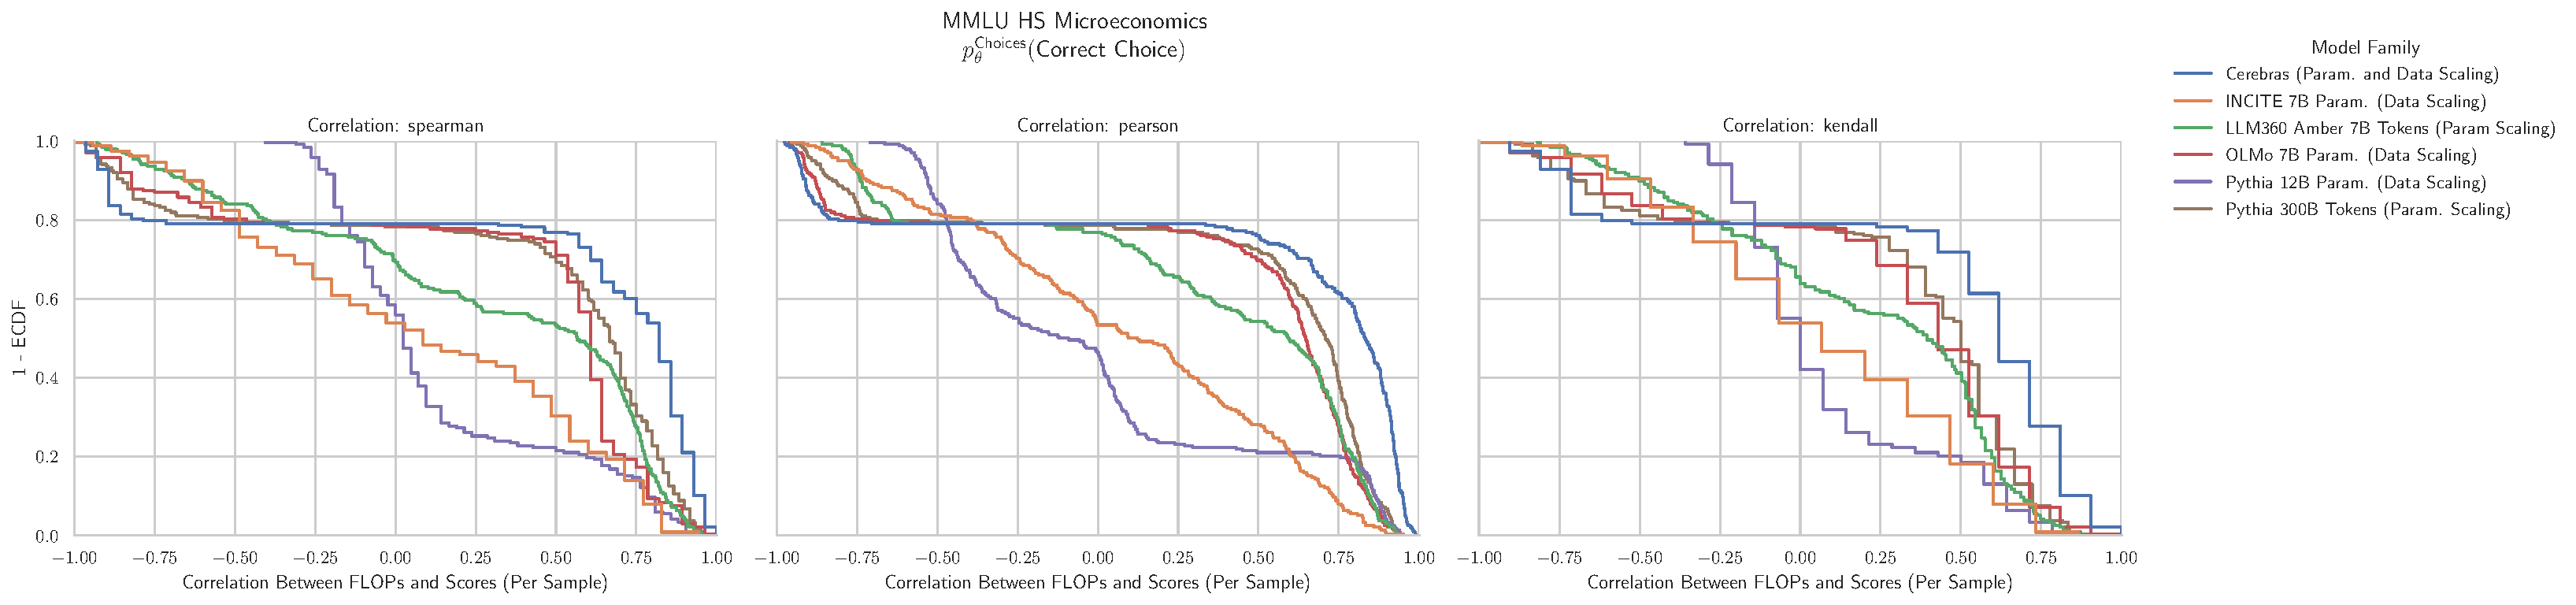
\includegraphics[width=\textwidth]{figures/correlations_between_scores_and_compute/correlation_distributions/mmlu_high_school_microeconomics/mmlu_high_school_microeconomics_prob_correct_choices_ecdf_vs_correlation_score_by_modelfamily_split_correlation_metric.pdf}
    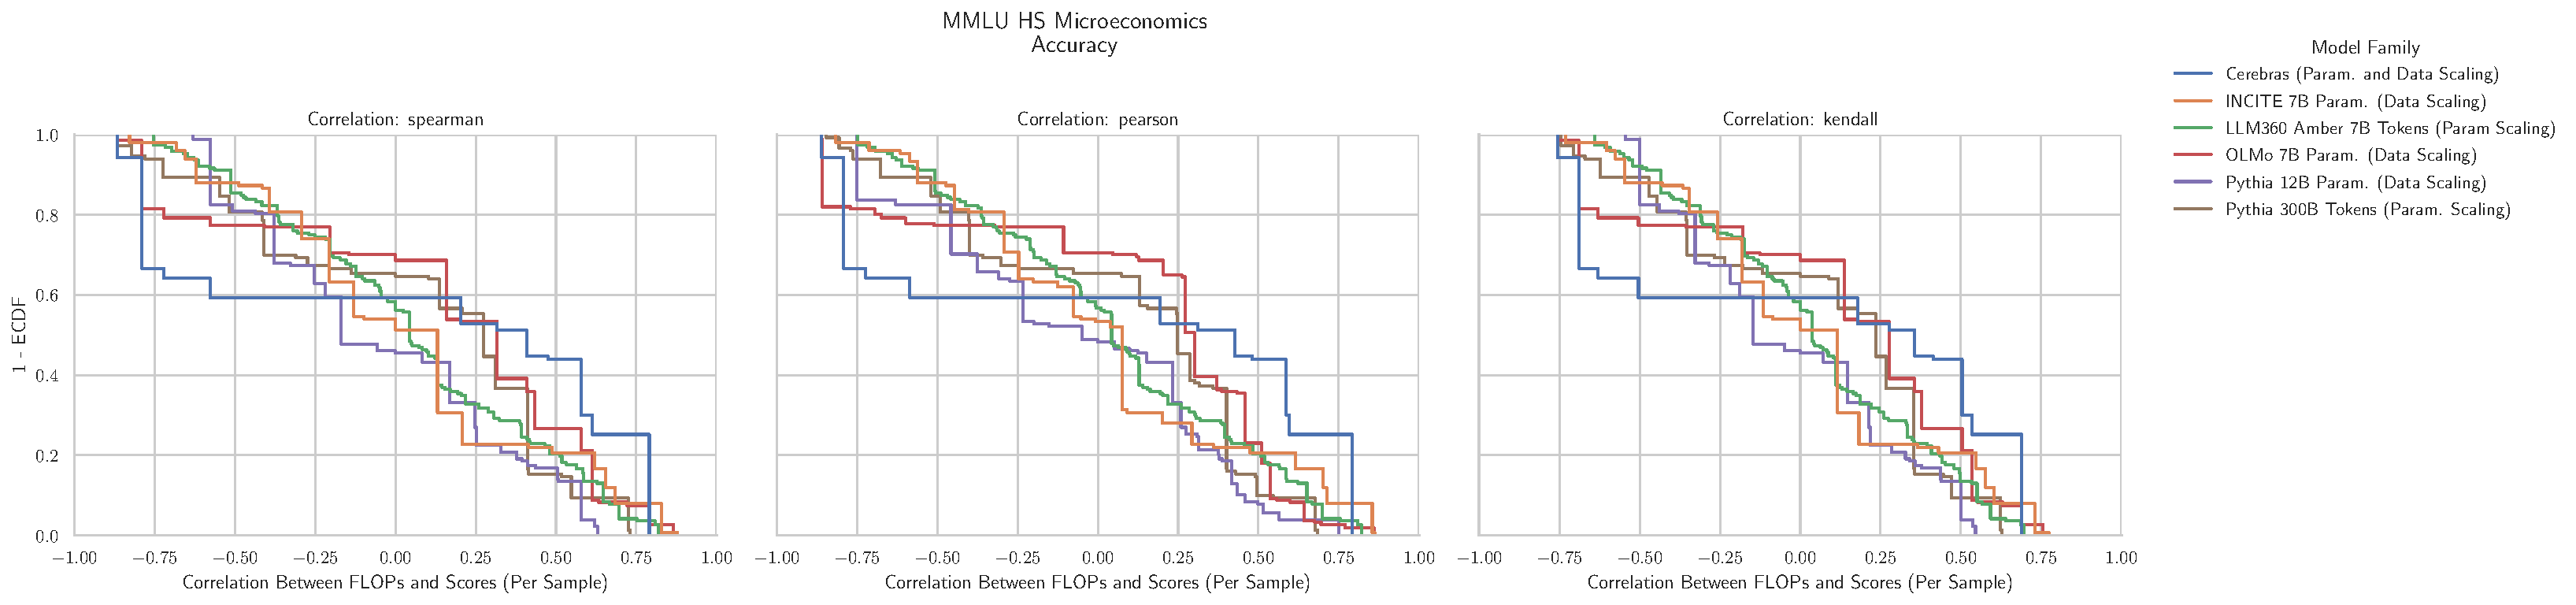
\includegraphics[width=\textwidth]{figures/correlations_between_scores_and_compute/correlation_distributions/mmlu_high_school_microeconomics/mmlu_high_school_microeconomics_acc_ecdf_vs_correlation_score_by_modelfamily_split_correlation_metric.pdf}
    \caption{\textbf{MMLU High School Microeconomics: Downstream performance is computed via a sequence of transformations that deteriorate correlations between scores and pretraining compute.}}
    \label{app:fig:compute_score_distribution_mmlu_high_school_microeconomics}
\end{figure}


\clearpage
\subsection{NLP Benchmark: MMLU High School Physics \cite{hendrycks2020mmlu}}

\begin{figure}[h!]
    \centering
    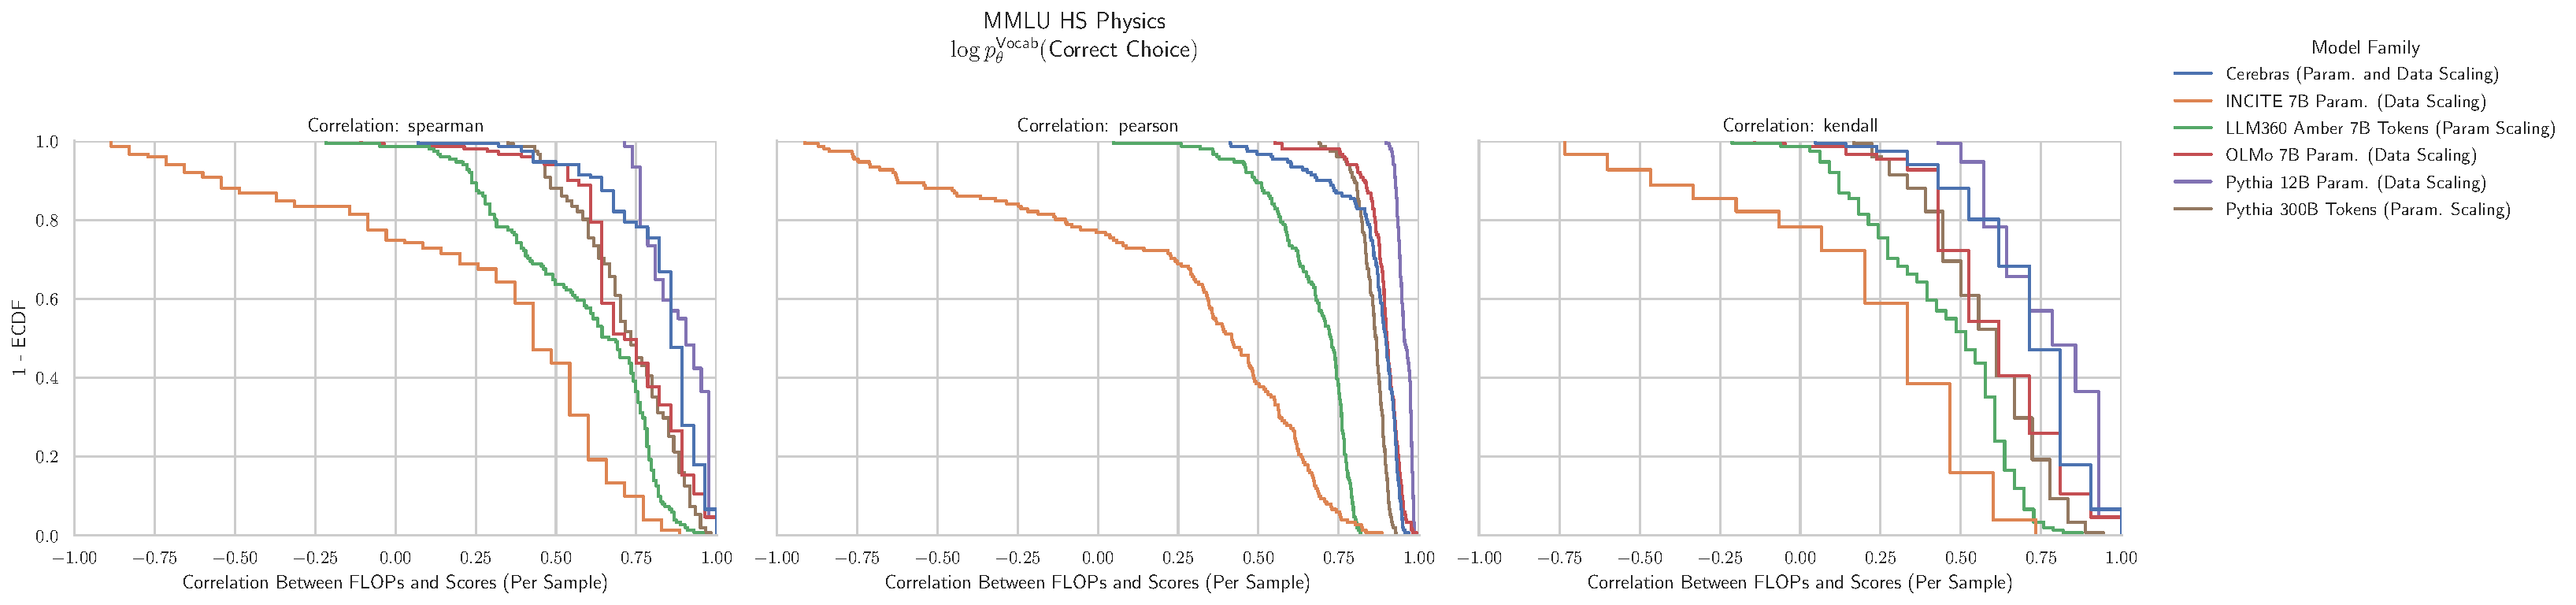
\includegraphics[width=\textwidth]{figures/correlations_between_scores_and_compute/correlation_distributions/mmlu_high_school_physics/mmlu_high_school_physics_log_likelihood_correct_ecdf_vs_correlation_score_by_modelfamily_split_correlation_metric.pdf}
    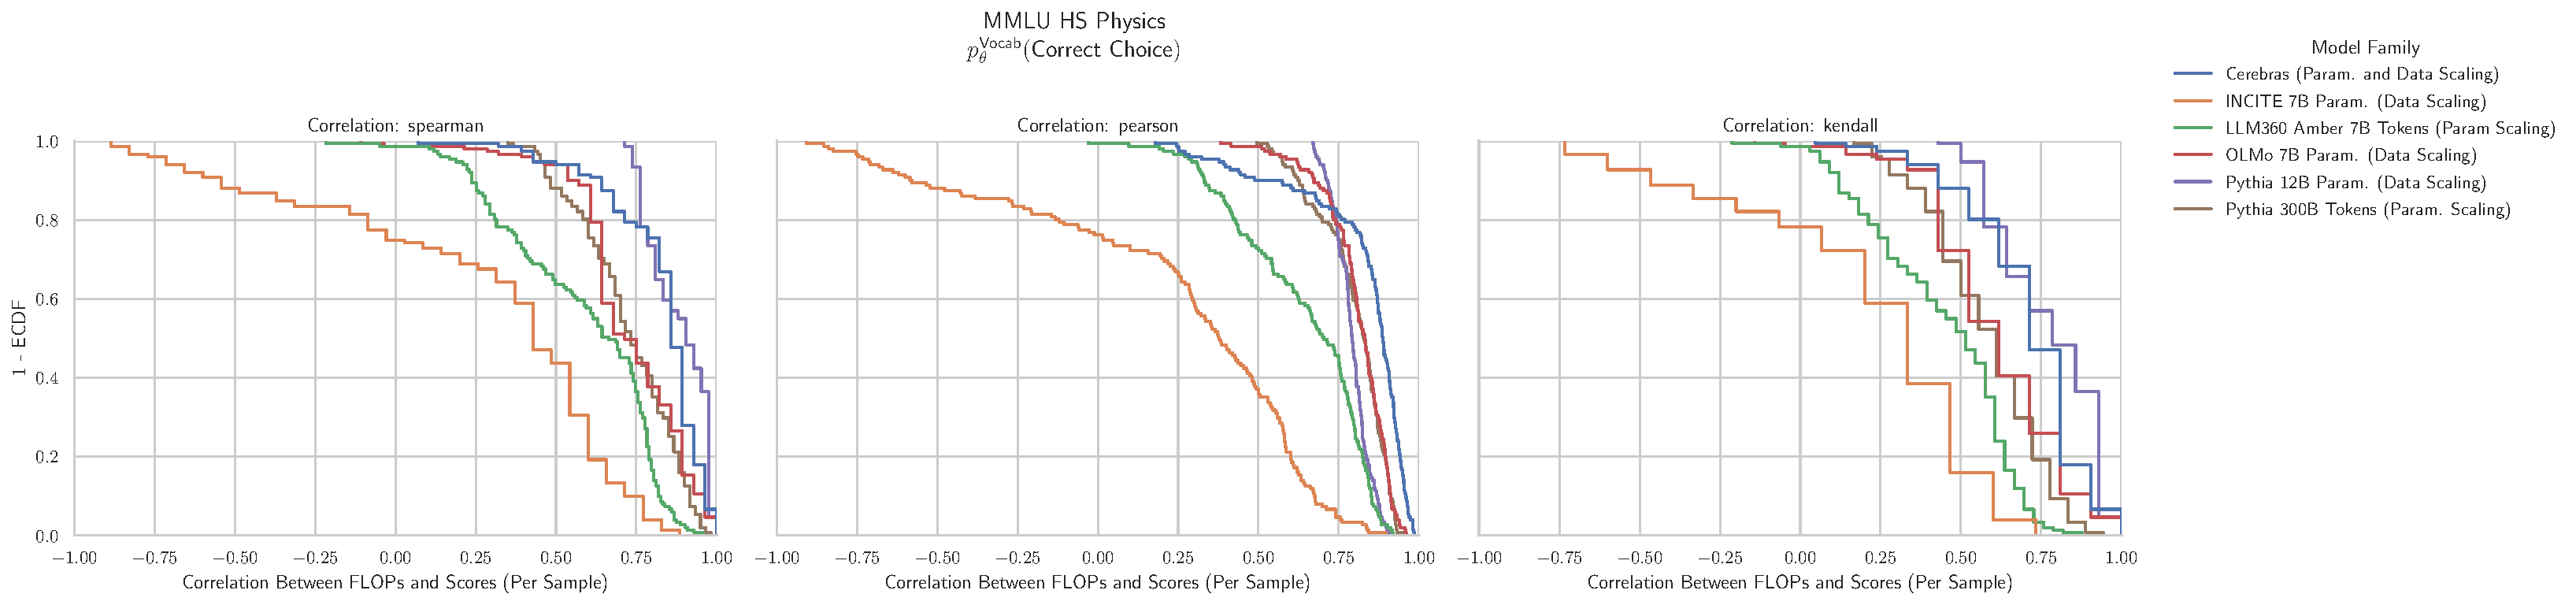
\includegraphics[width=\textwidth]{figures/correlations_between_scores_and_compute/correlation_distributions/mmlu_high_school_physics/mmlu_high_school_physics_prob_correct_vocab_ecdf_vs_correlation_score_by_modelfamily_split_correlation_metric.pdf}
    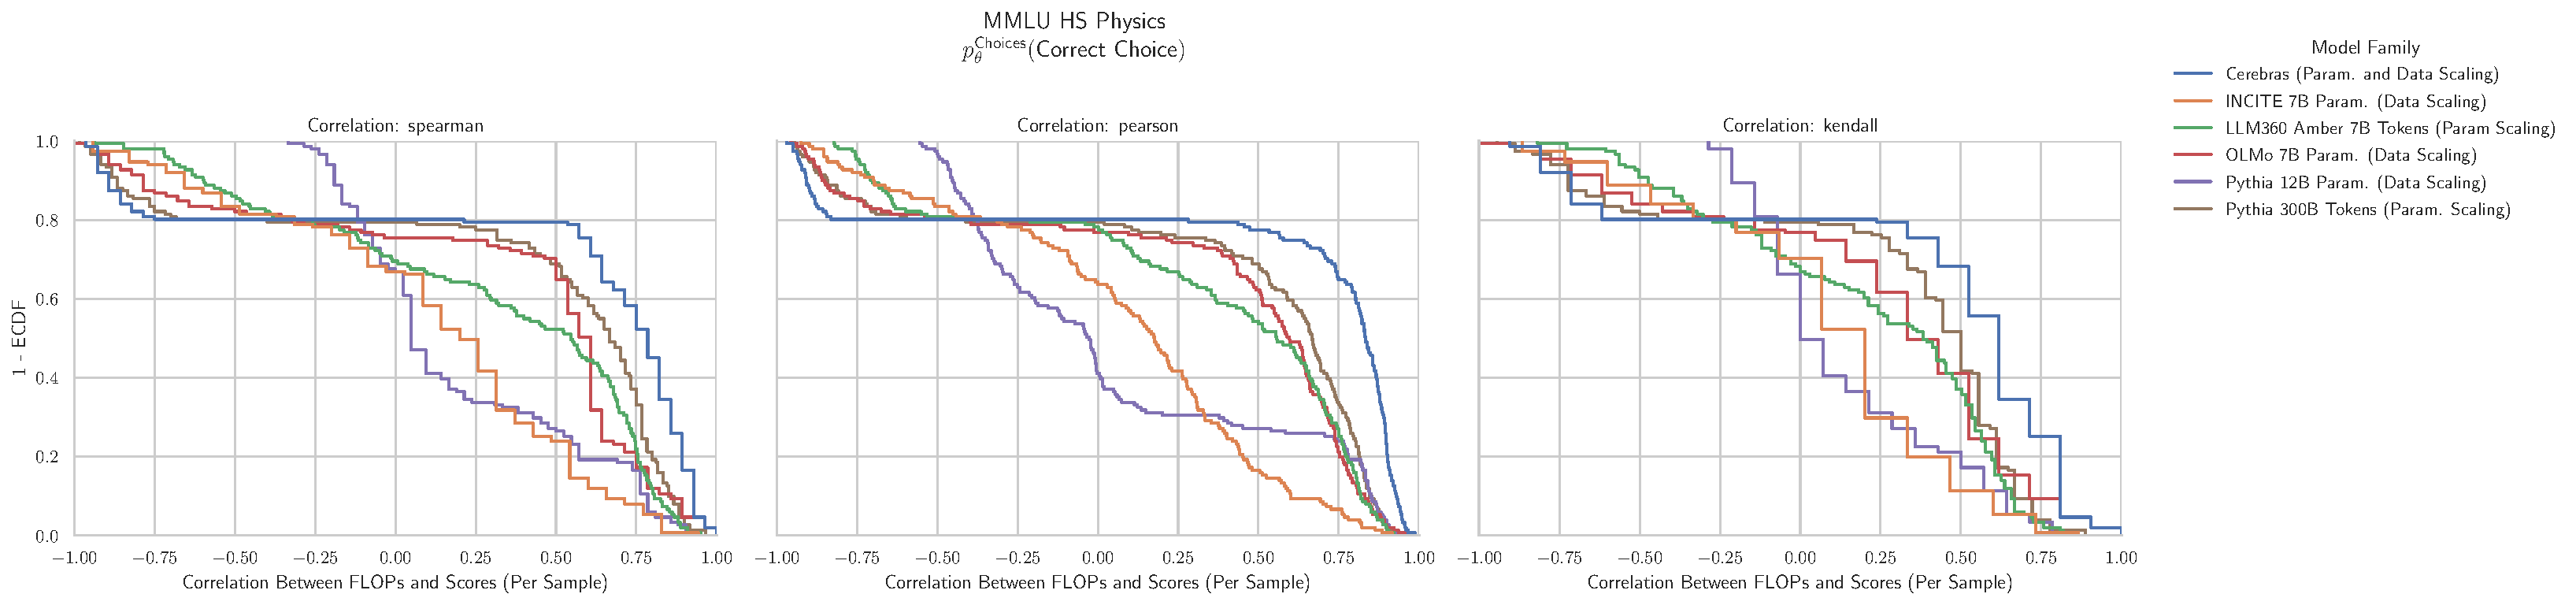
\includegraphics[width=\textwidth]{figures/correlations_between_scores_and_compute/correlation_distributions/mmlu_high_school_physics/mmlu_high_school_physics_prob_correct_choices_ecdf_vs_correlation_score_by_modelfamily_split_correlation_metric.pdf}
    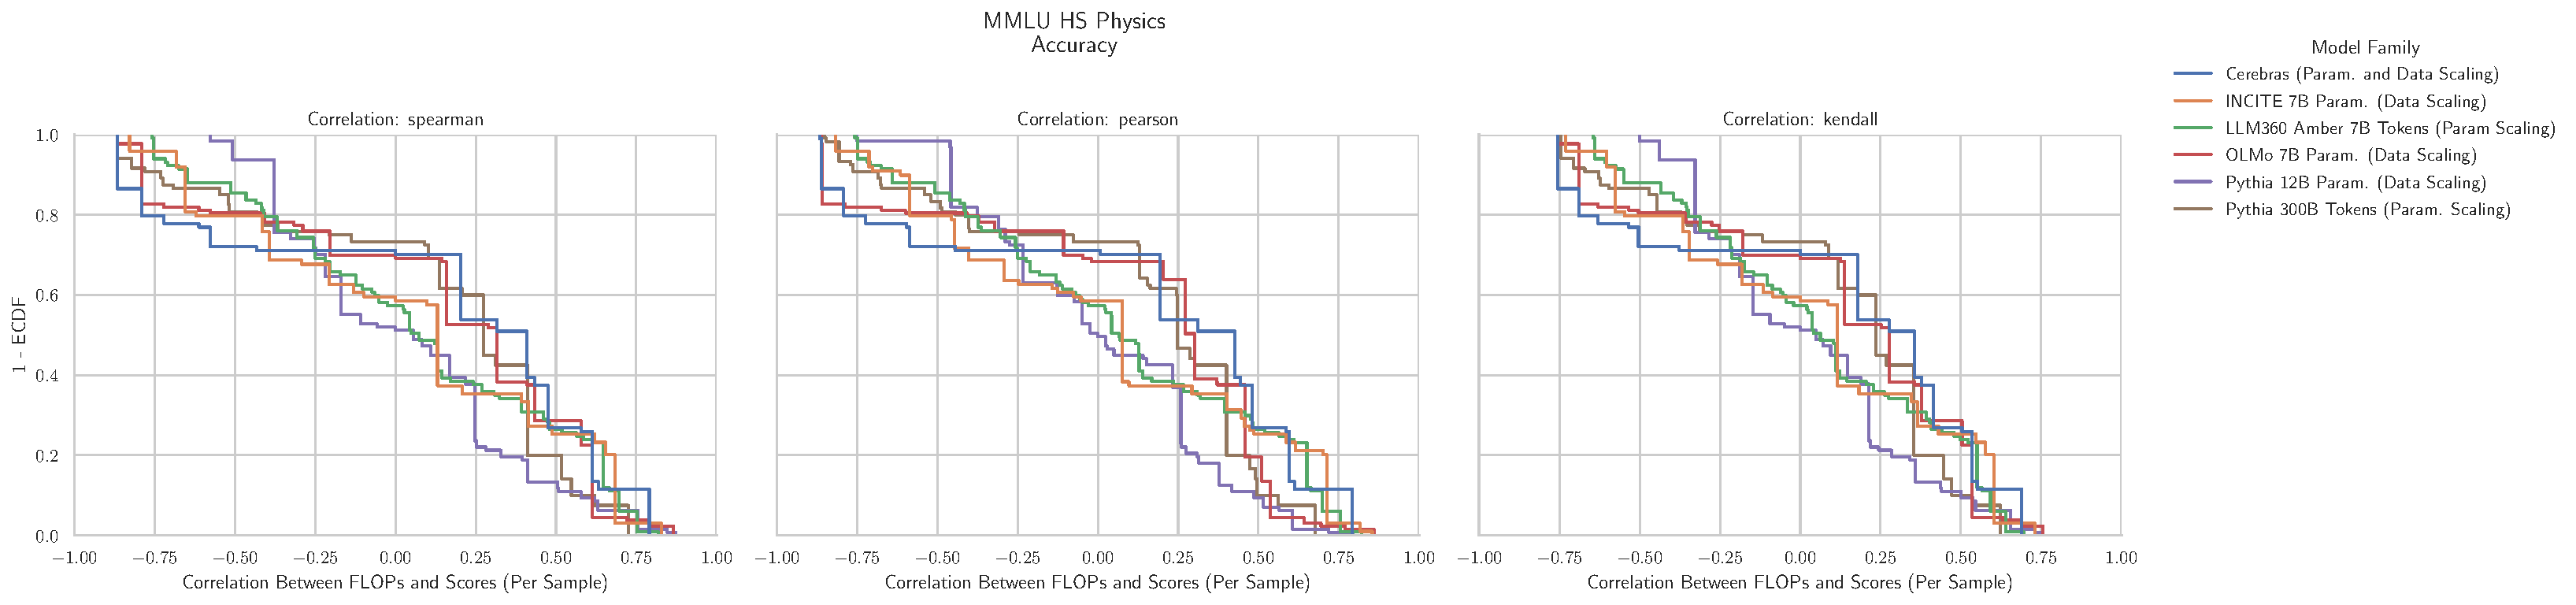
\includegraphics[width=\textwidth]{figures/correlations_between_scores_and_compute/correlation_distributions/mmlu_high_school_physics/mmlu_high_school_physics_acc_ecdf_vs_correlation_score_by_modelfamily_split_correlation_metric.pdf}
    \caption{\textbf{MMLU High School Physics: Downstream performance is computed via a sequence of transformations that deteriorate correlations between scores and pretraining compute.}}
    \label{app:fig:compute_score_distribution_mmlu_high_school_physics}
\end{figure}


\clearpage
\subsection{NLP Benchmark: MMLU High School Psychology \cite{hendrycks2020mmlu}}

\begin{figure}[h!]
    \centering
    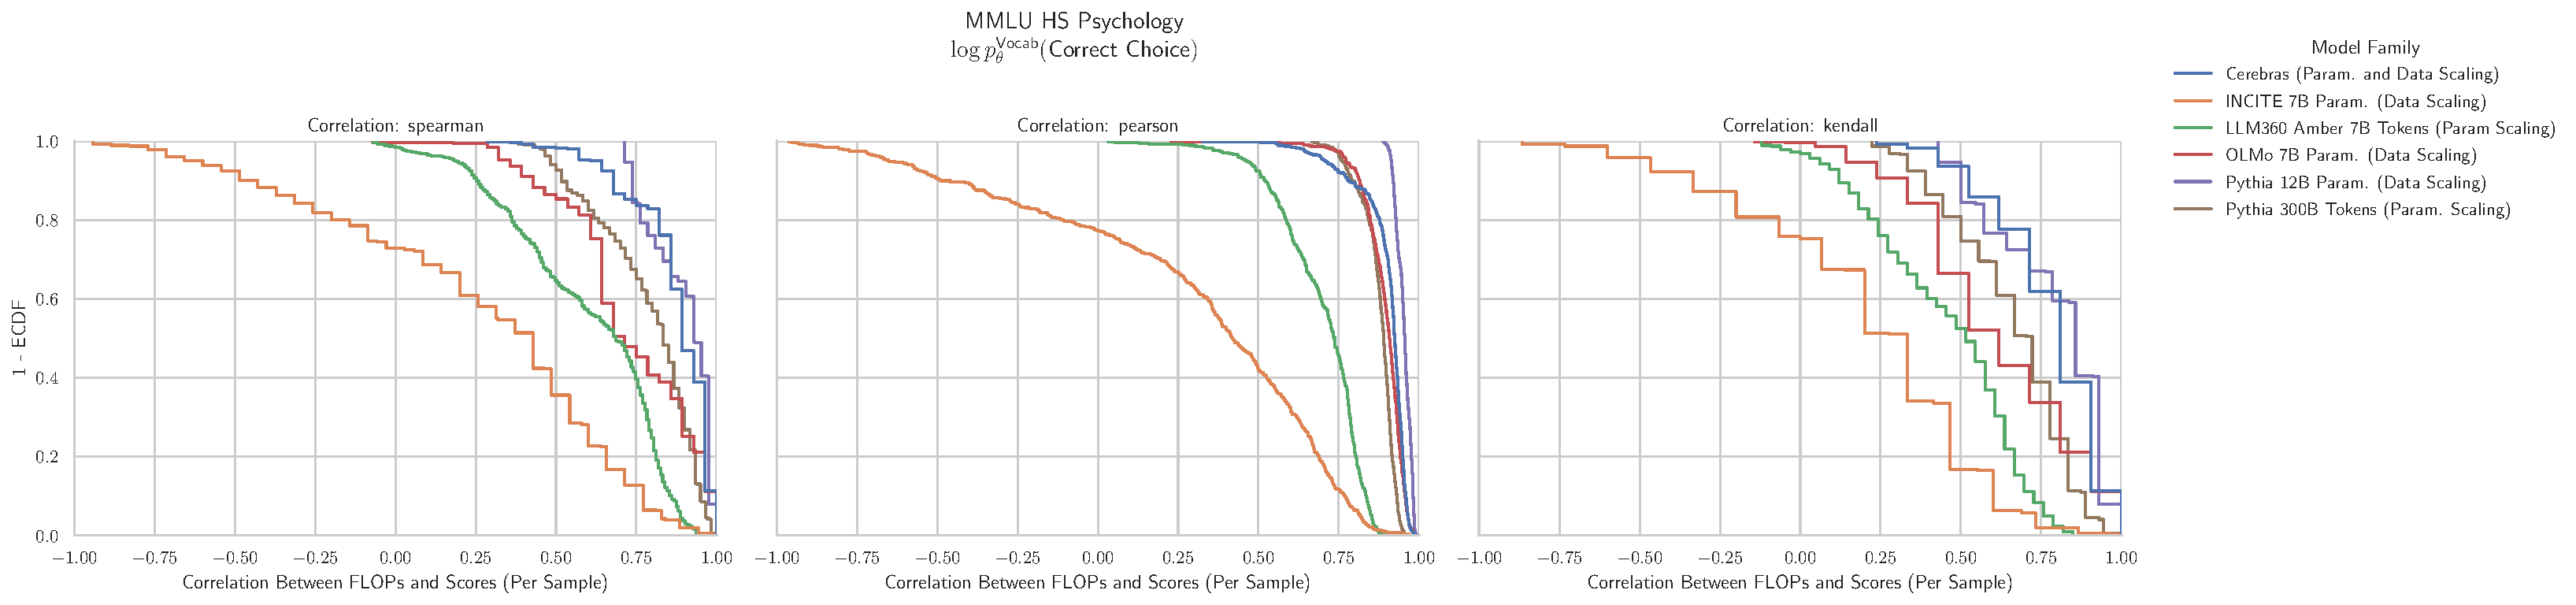
\includegraphics[width=\textwidth]{figures/correlations_between_scores_and_compute/correlation_distributions/mmlu_high_school_psychology/mmlu_high_school_psychology_log_likelihood_correct_ecdf_vs_correlation_score_by_modelfamily_split_correlation_metric.pdf}
    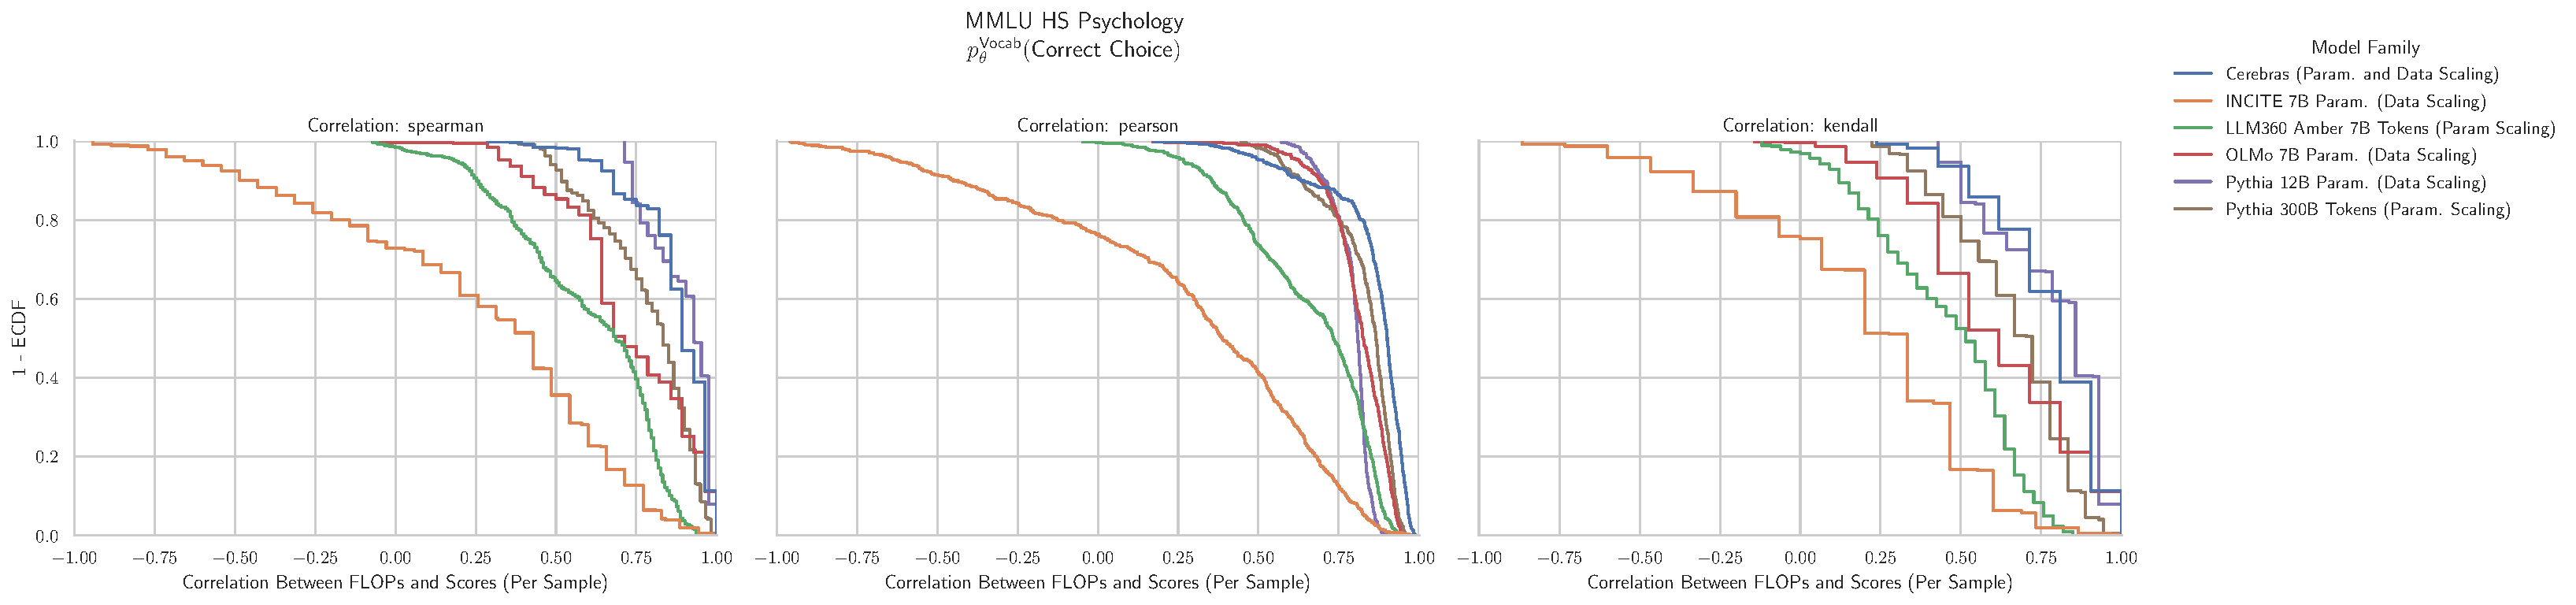
\includegraphics[width=\textwidth]{figures/correlations_between_scores_and_compute/correlation_distributions/mmlu_high_school_psychology/mmlu_high_school_psychology_prob_correct_vocab_ecdf_vs_correlation_score_by_modelfamily_split_correlation_metric.pdf}
    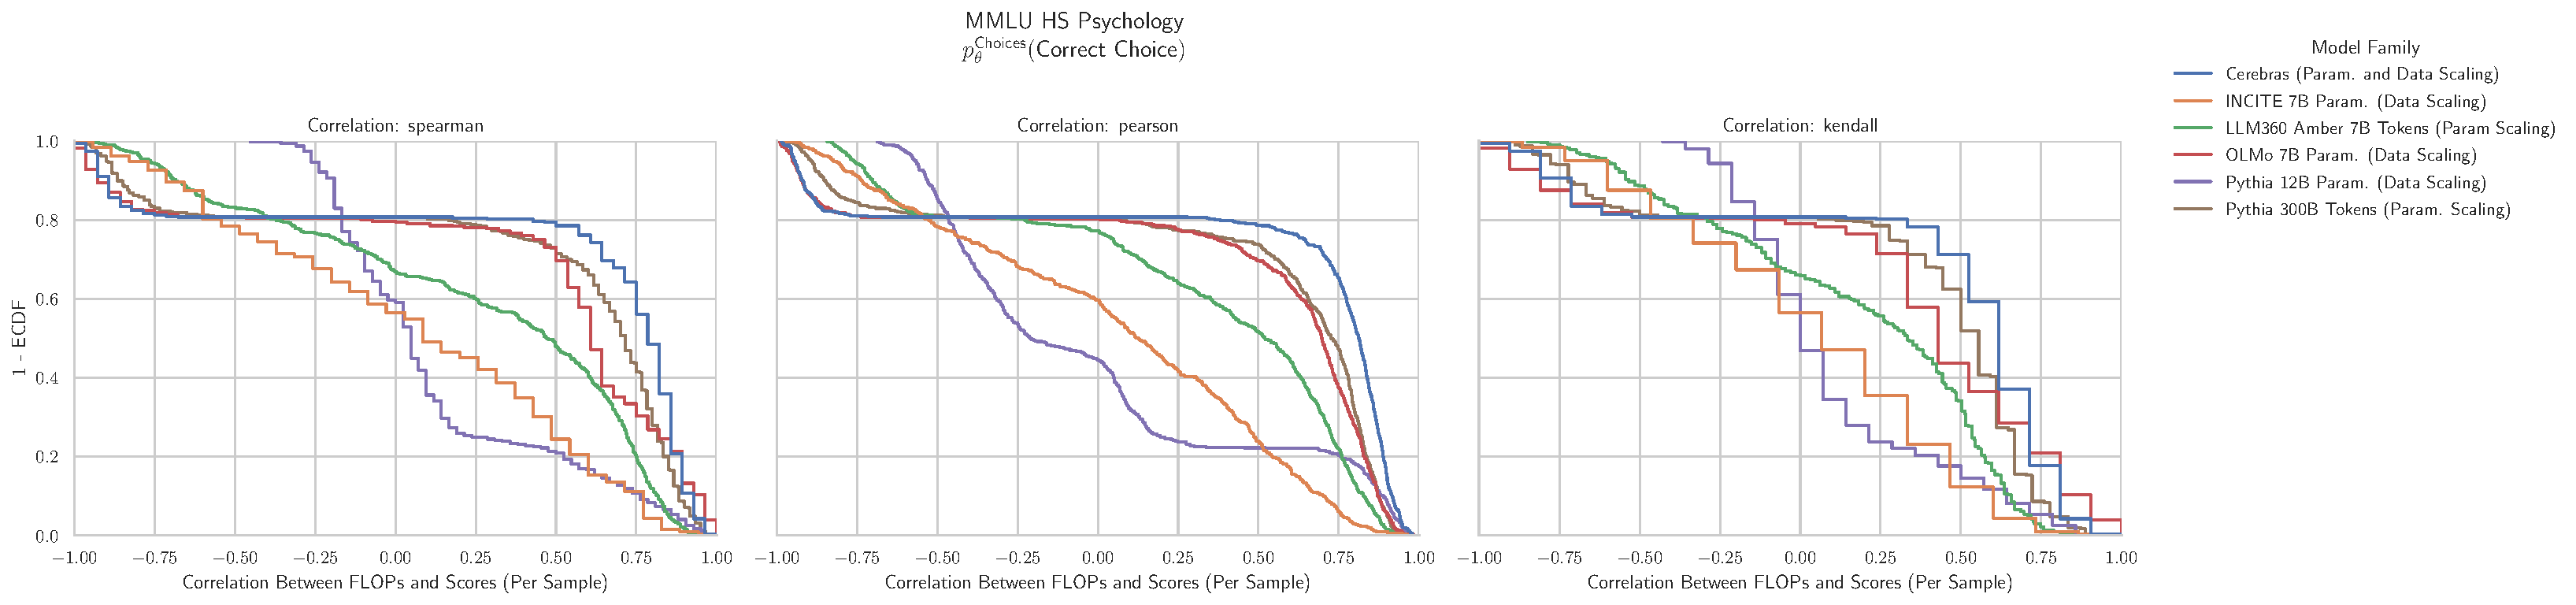
\includegraphics[width=\textwidth]{figures/correlations_between_scores_and_compute/correlation_distributions/mmlu_high_school_psychology/mmlu_high_school_psychology_prob_correct_choices_ecdf_vs_correlation_score_by_modelfamily_split_correlation_metric.pdf}
    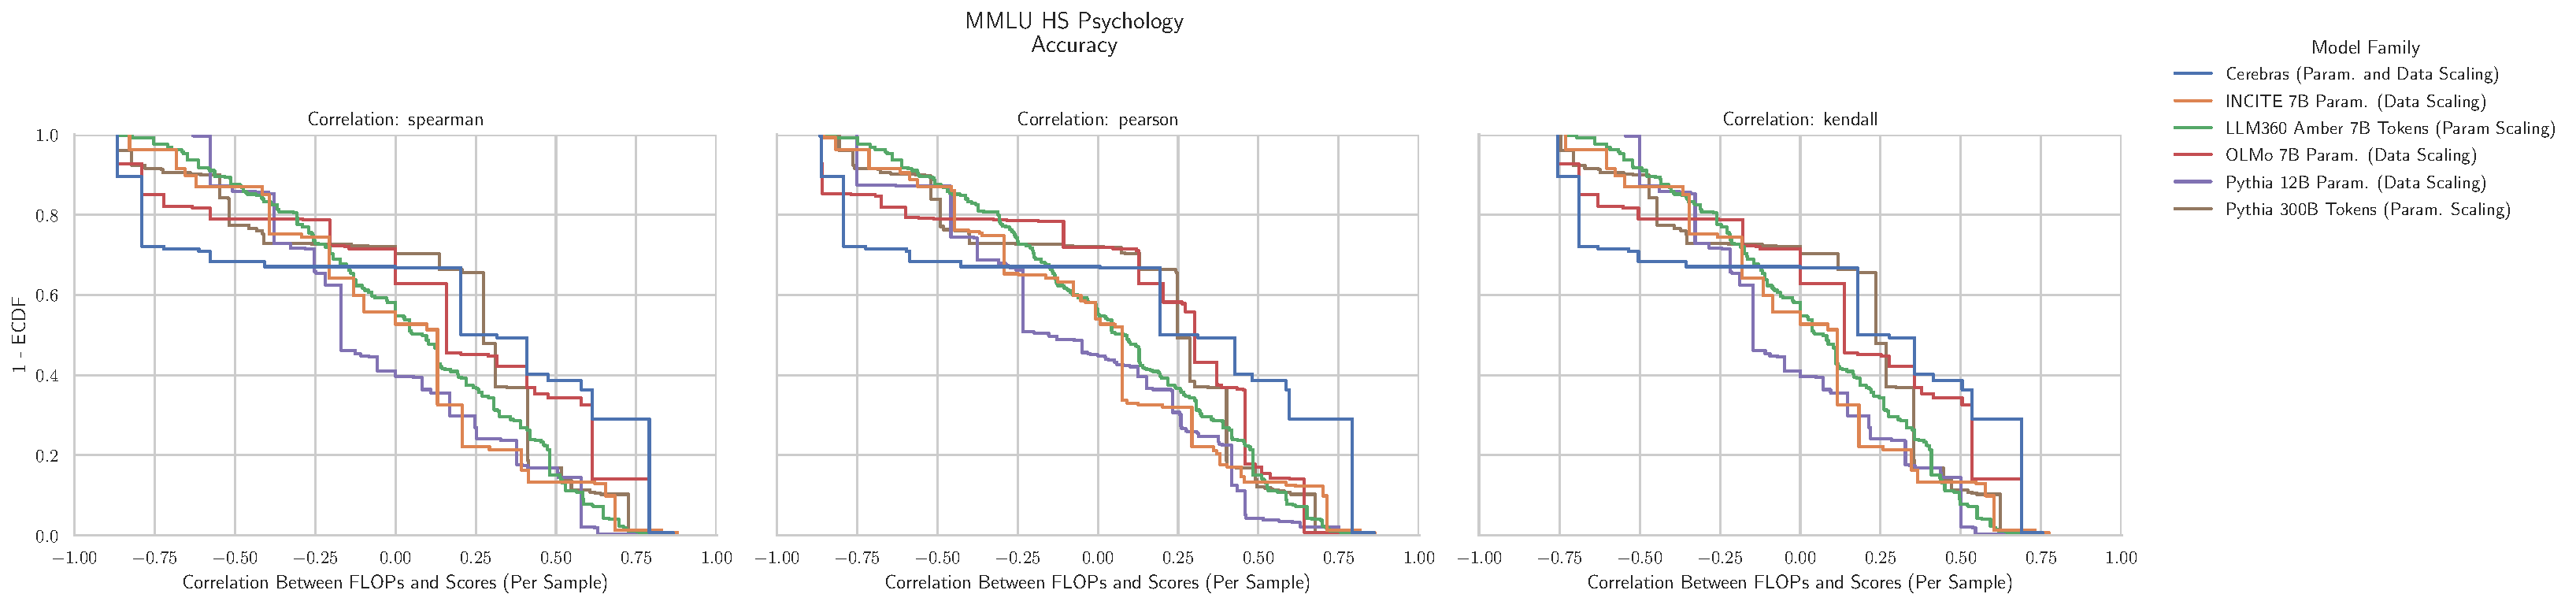
\includegraphics[width=\textwidth]{figures/correlations_between_scores_and_compute/correlation_distributions/mmlu_high_school_psychology/mmlu_high_school_psychology_acc_ecdf_vs_correlation_score_by_modelfamily_split_correlation_metric.pdf}
    \caption{\textbf{MMLU High School Psychology: Downstream performance is computed via a sequence of transformations that deteriorate correlations between scores and pretraining compute.}}
    \label{app:fig:compute_score_distribution_mmlu_high_school_psychology}
\end{figure}


\clearpage
\subsection{NLP Benchmark: MMLU High School Statistics \cite{hendrycks2020mmlu}}

\begin{figure}[h!]
    \centering
    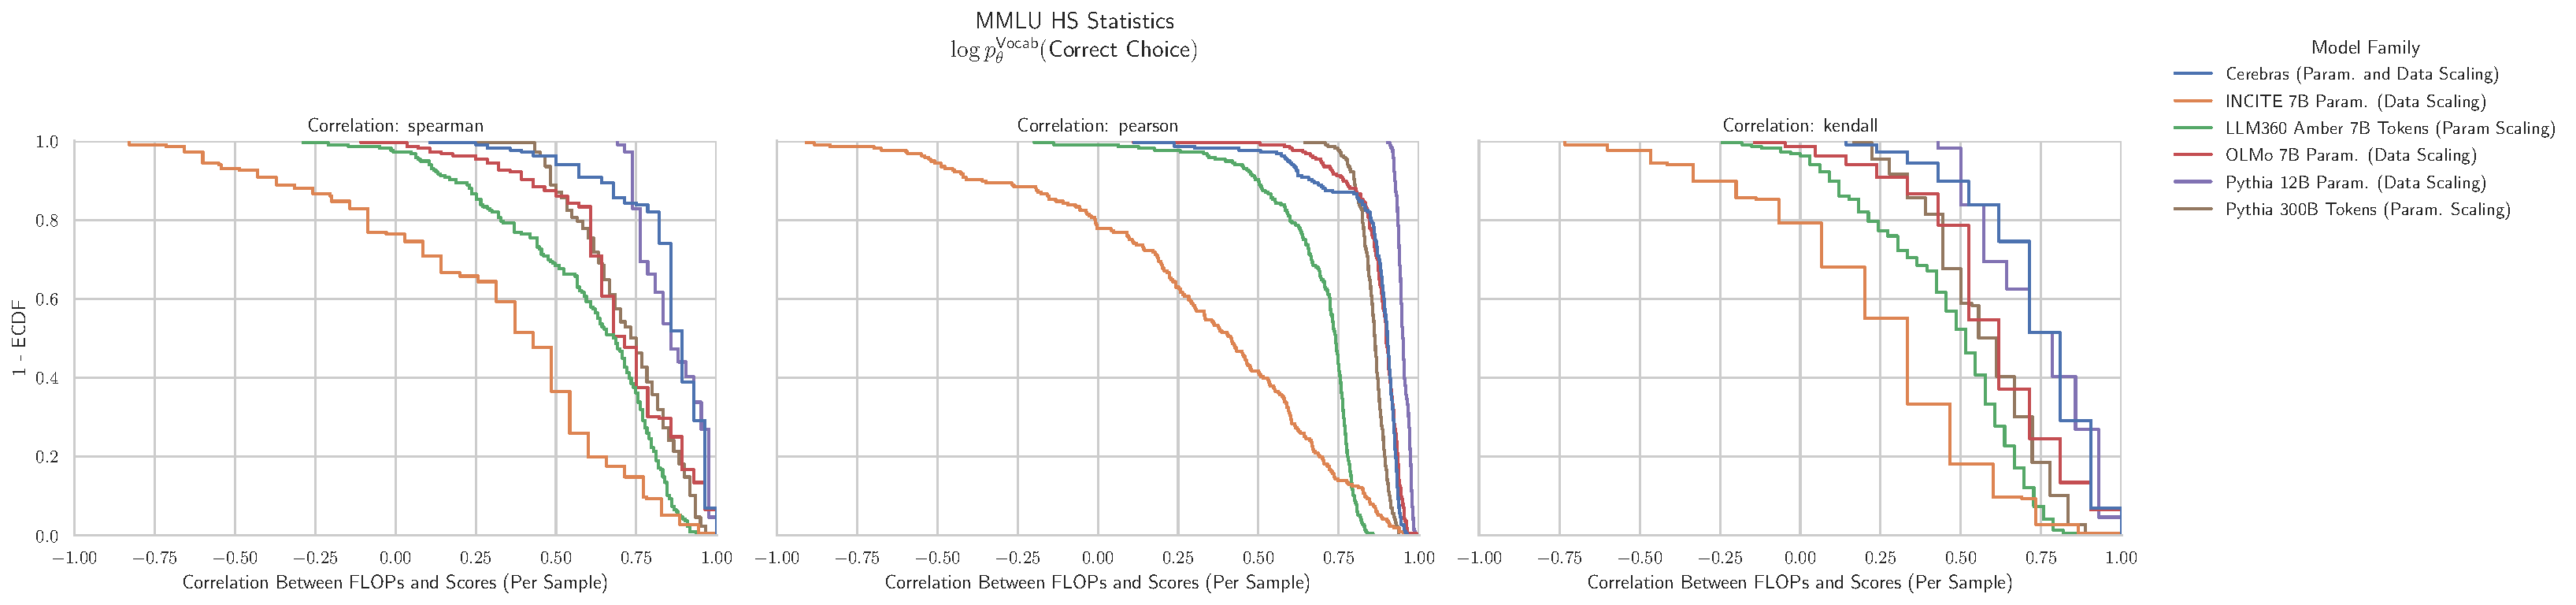
\includegraphics[width=\textwidth]{figures/correlations_between_scores_and_compute/correlation_distributions/mmlu_high_school_statistics/mmlu_high_school_statistics_log_likelihood_correct_ecdf_vs_correlation_score_by_modelfamily_split_correlation_metric.pdf}
    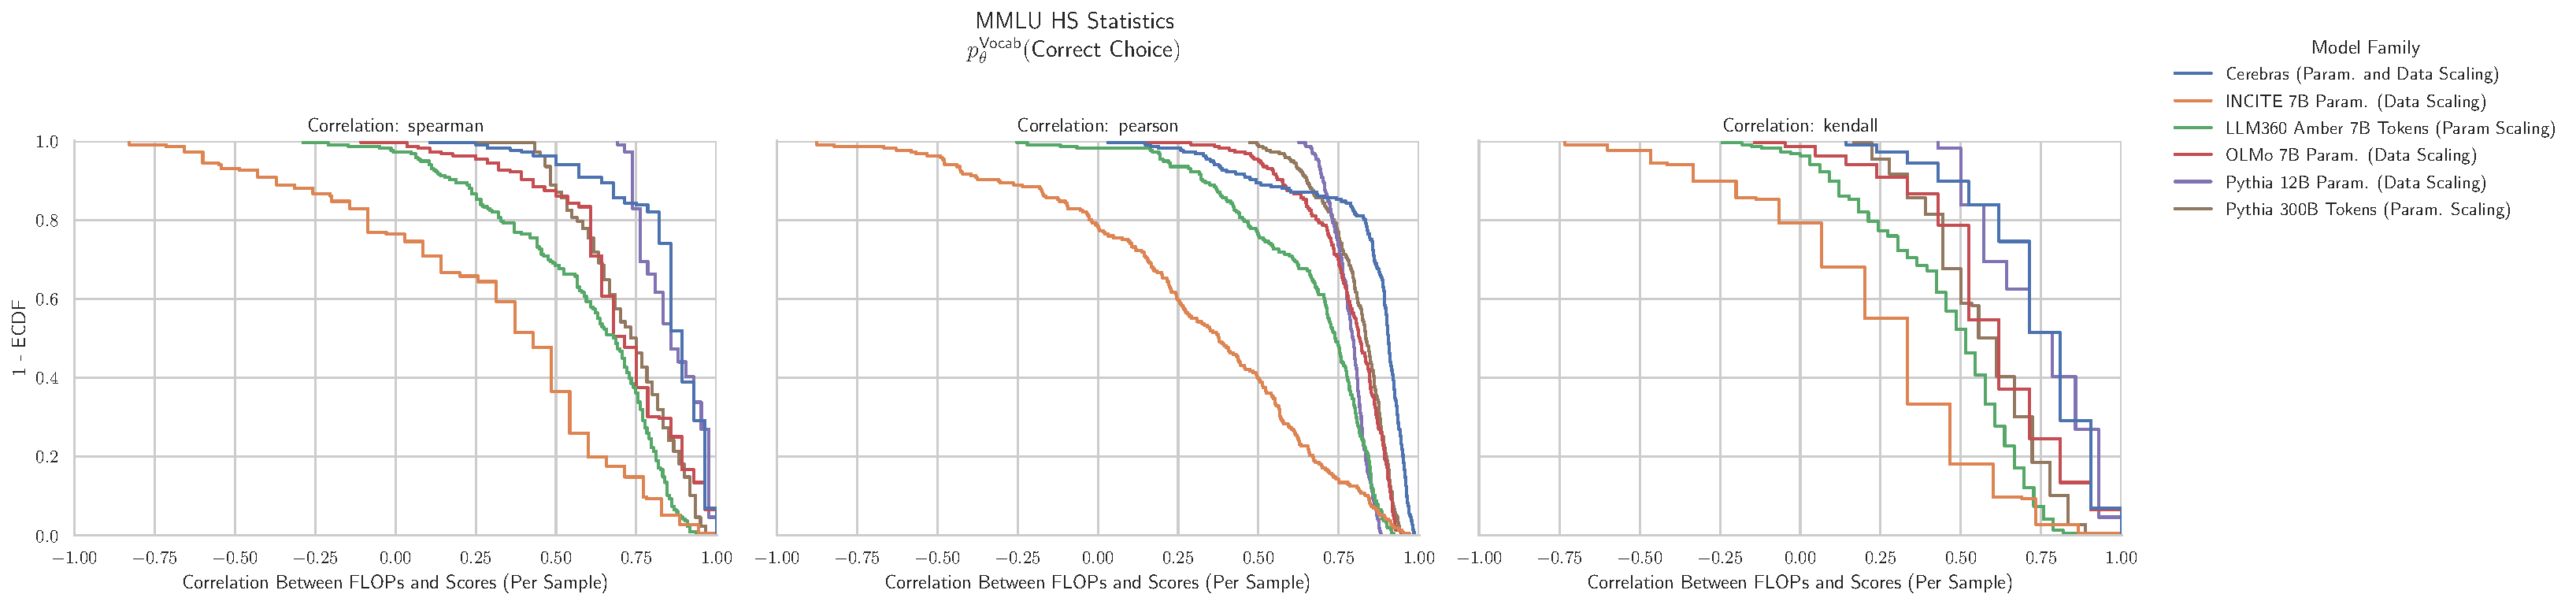
\includegraphics[width=\textwidth]{figures/correlations_between_scores_and_compute/correlation_distributions/mmlu_high_school_statistics/mmlu_high_school_statistics_prob_correct_vocab_ecdf_vs_correlation_score_by_modelfamily_split_correlation_metric.pdf}
    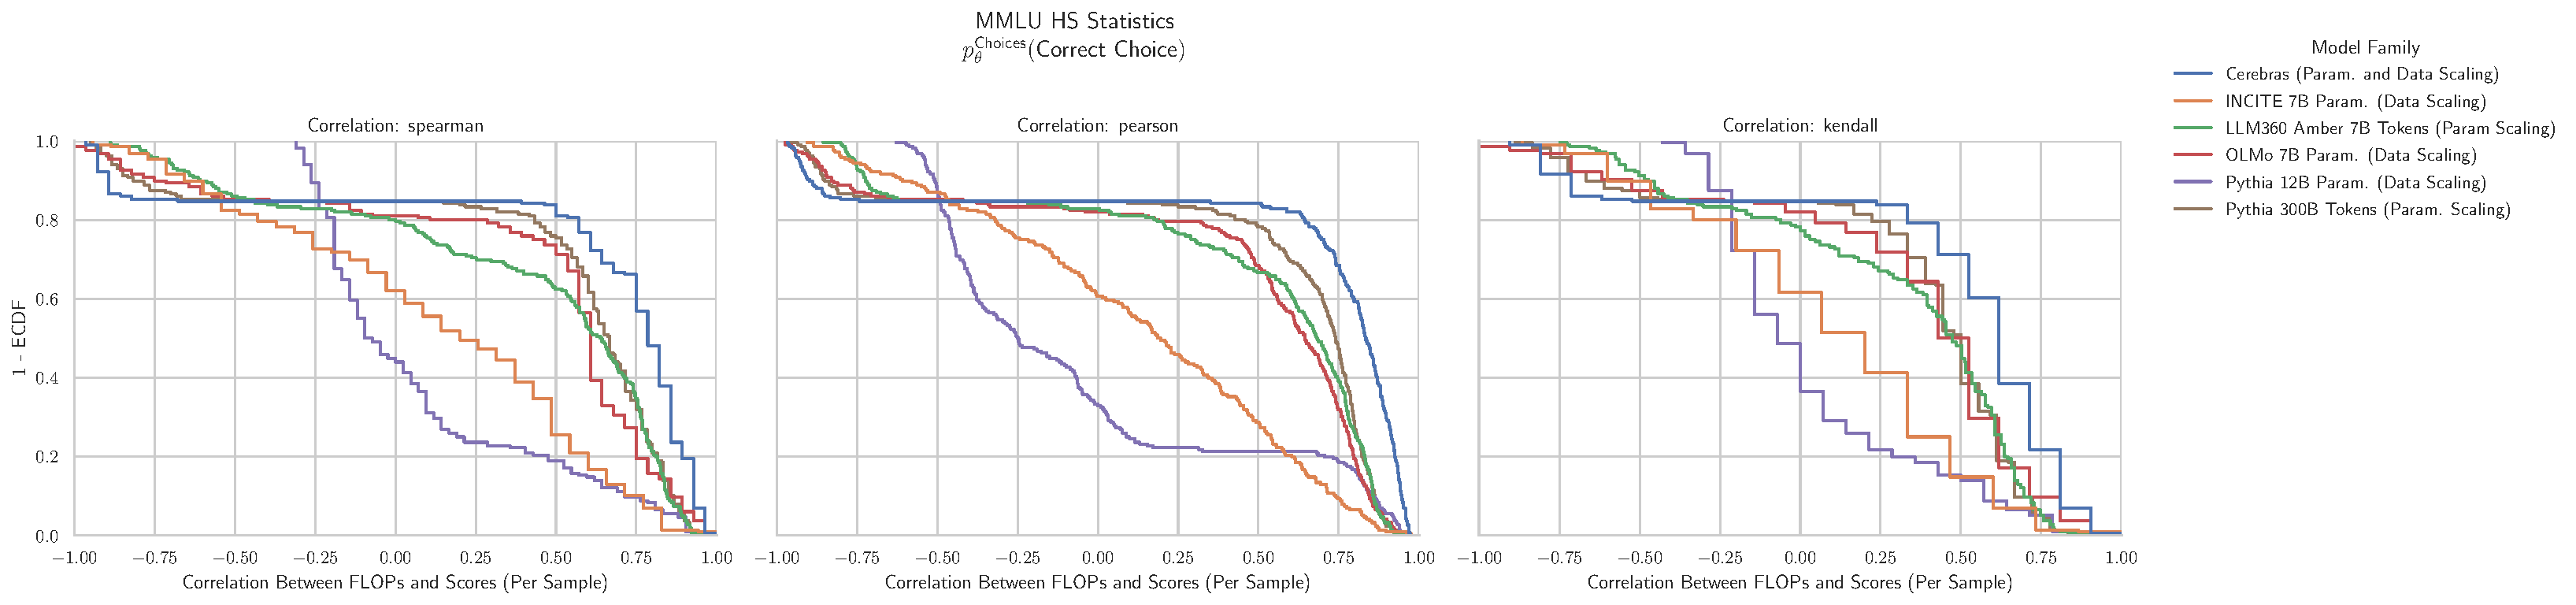
\includegraphics[width=\textwidth]{figures/correlations_between_scores_and_compute/correlation_distributions/mmlu_high_school_statistics/mmlu_high_school_statistics_prob_correct_choices_ecdf_vs_correlation_score_by_modelfamily_split_correlation_metric.pdf}
    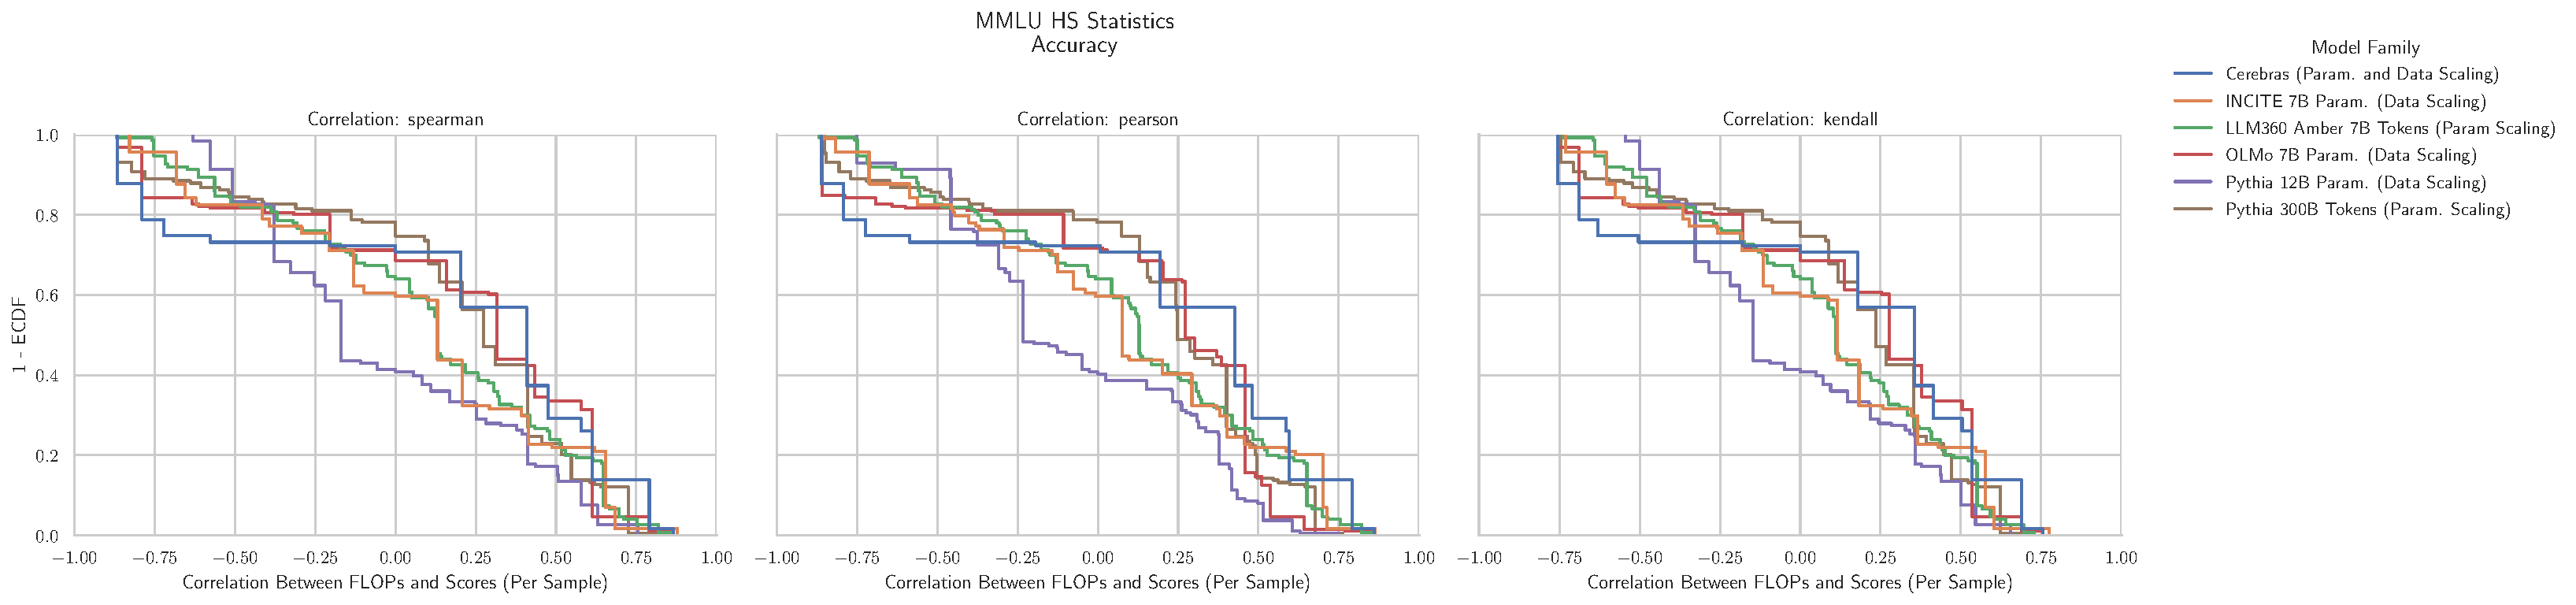
\includegraphics[width=\textwidth]{figures/correlations_between_scores_and_compute/correlation_distributions/mmlu_high_school_statistics/mmlu_high_school_statistics_acc_ecdf_vs_correlation_score_by_modelfamily_split_correlation_metric.pdf}
    \caption{\textbf{MMLU High School Statistics: Downstream performance is computed via a sequence of transformations that deteriorate correlations between scores and pretraining compute.}}
    \label{app:fig:compute_score_distribution_mmlu_high_school_statistics}
\end{figure}


\clearpage
\subsection{NLP Benchmark: MMLU High School US History \cite{hendrycks2020mmlu}}

\begin{figure}[h!]
    \centering
    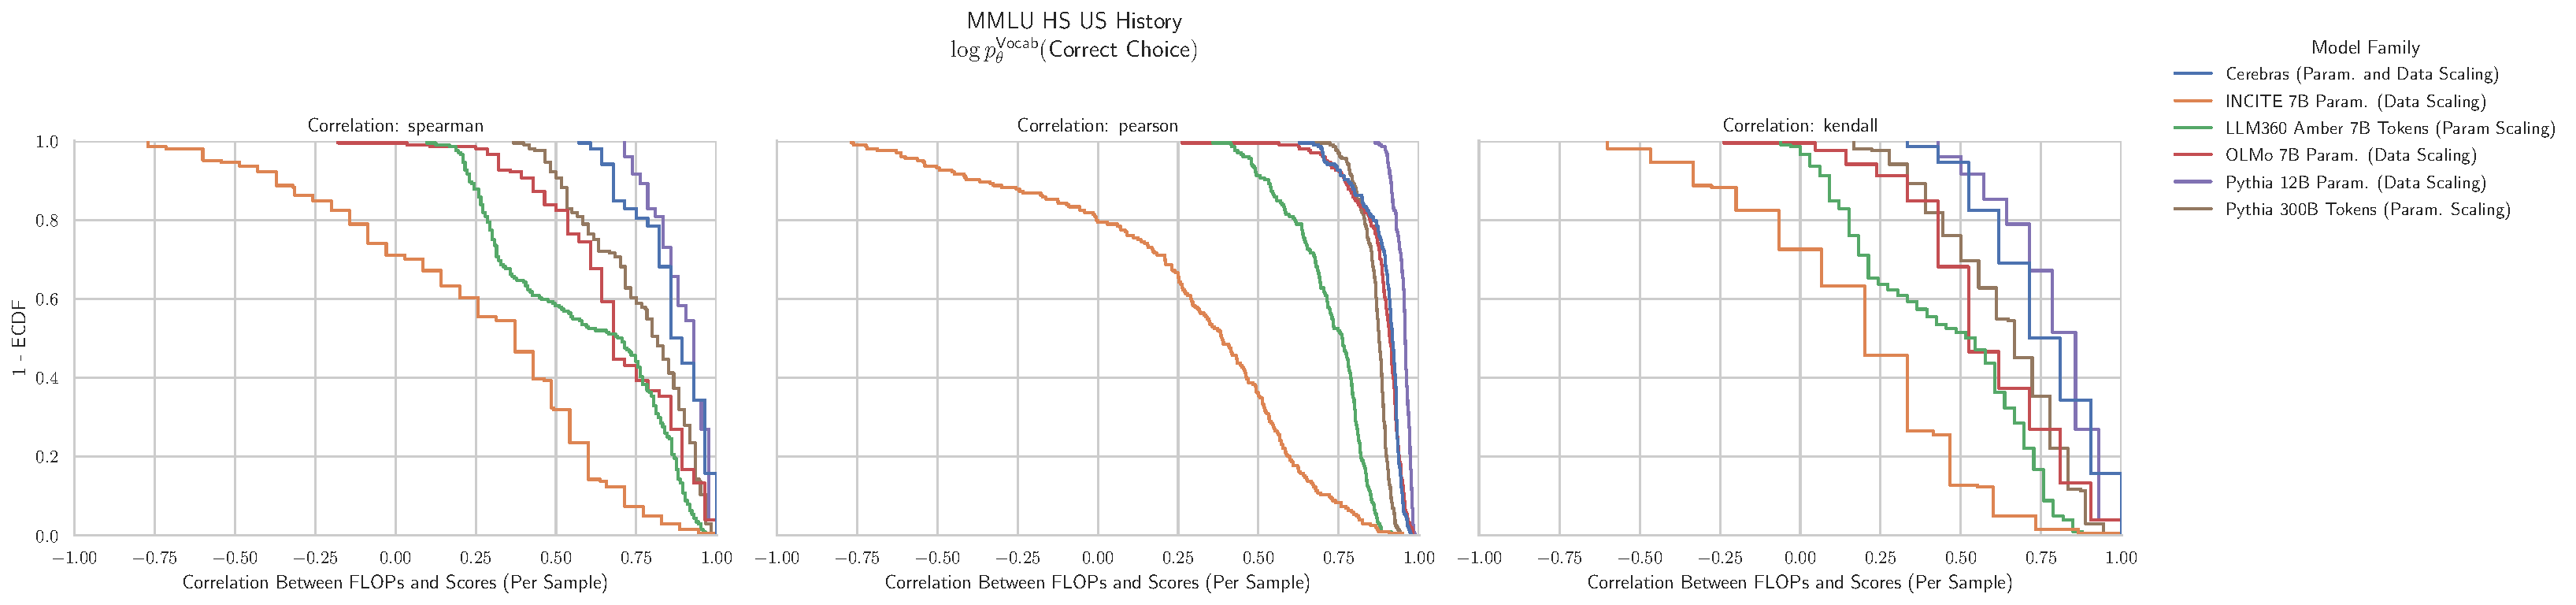
\includegraphics[width=\textwidth]{figures/correlations_between_scores_and_compute/correlation_distributions/mmlu_high_school_us_history/mmlu_high_school_us_history_log_likelihood_correct_ecdf_vs_correlation_score_by_modelfamily_split_correlation_metric.pdf}
    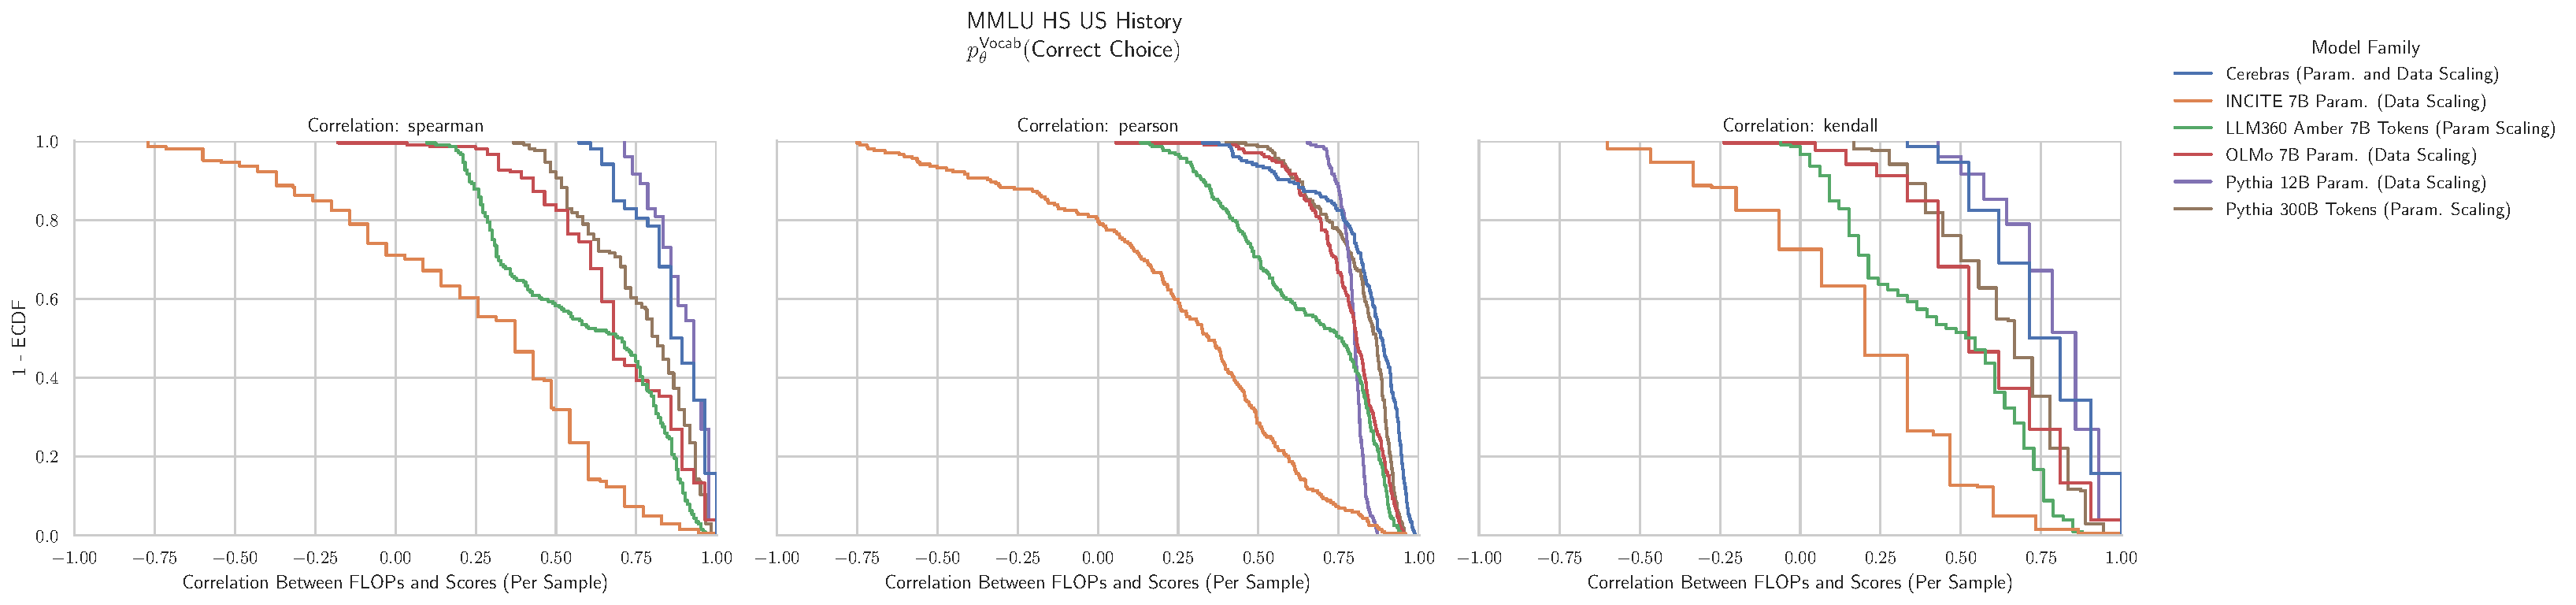
\includegraphics[width=\textwidth]{figures/correlations_between_scores_and_compute/correlation_distributions/mmlu_high_school_us_history/mmlu_high_school_us_history_prob_correct_vocab_ecdf_vs_correlation_score_by_modelfamily_split_correlation_metric.pdf}
    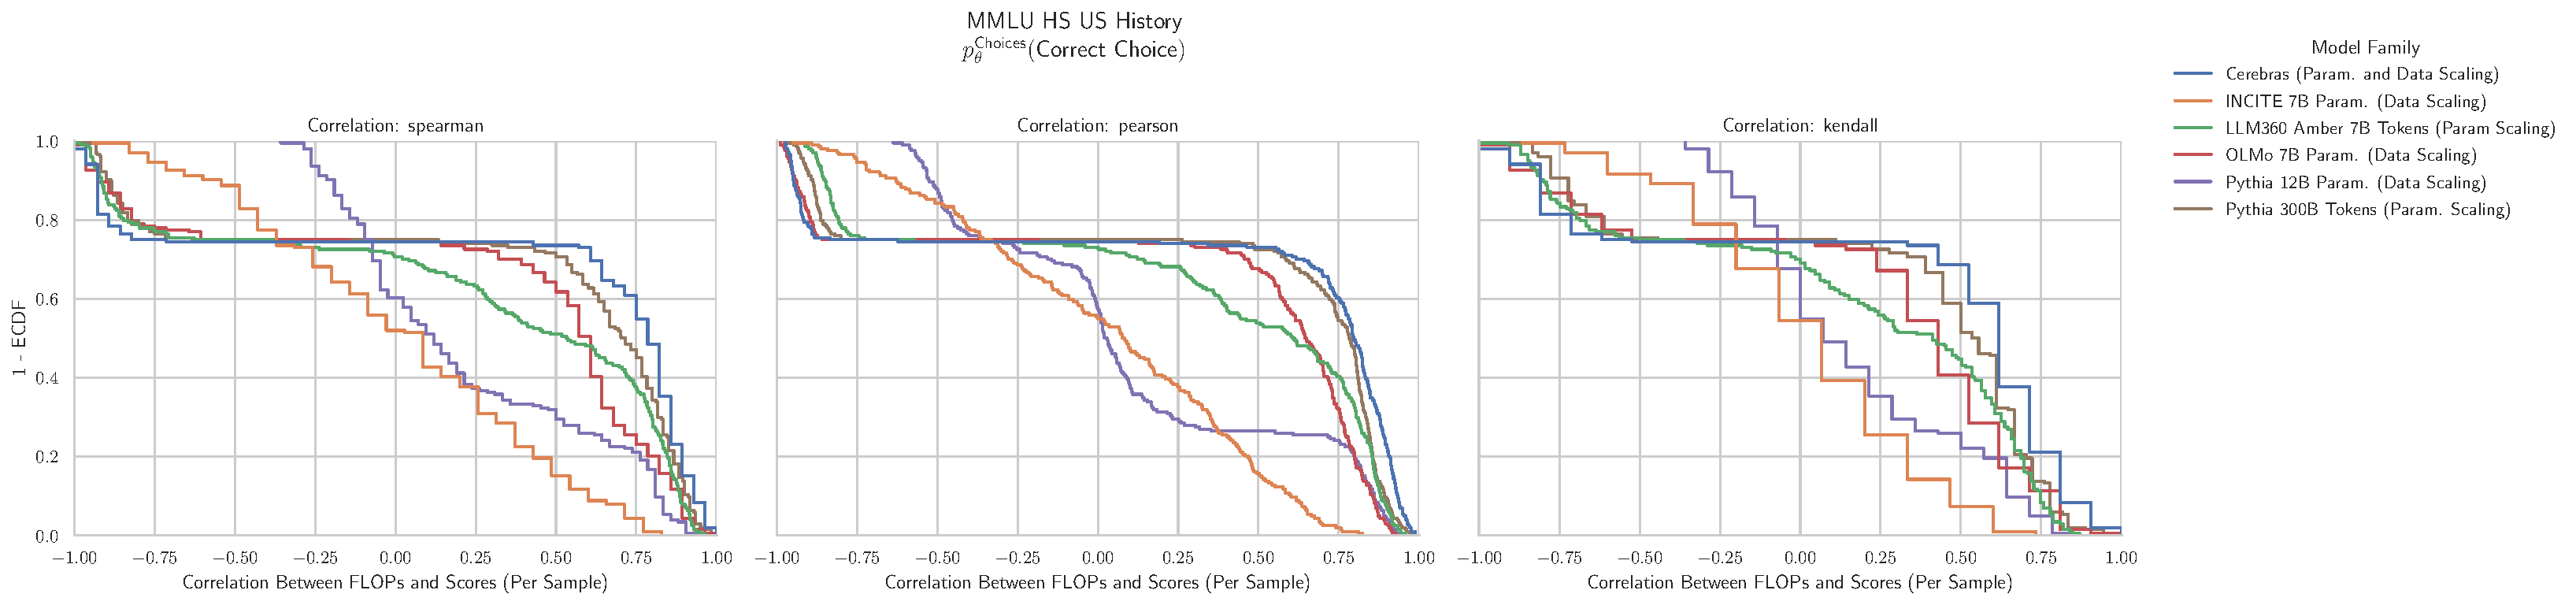
\includegraphics[width=\textwidth]{figures/correlations_between_scores_and_compute/correlation_distributions/mmlu_high_school_us_history/mmlu_high_school_us_history_prob_correct_choices_ecdf_vs_correlation_score_by_modelfamily_split_correlation_metric.pdf}
    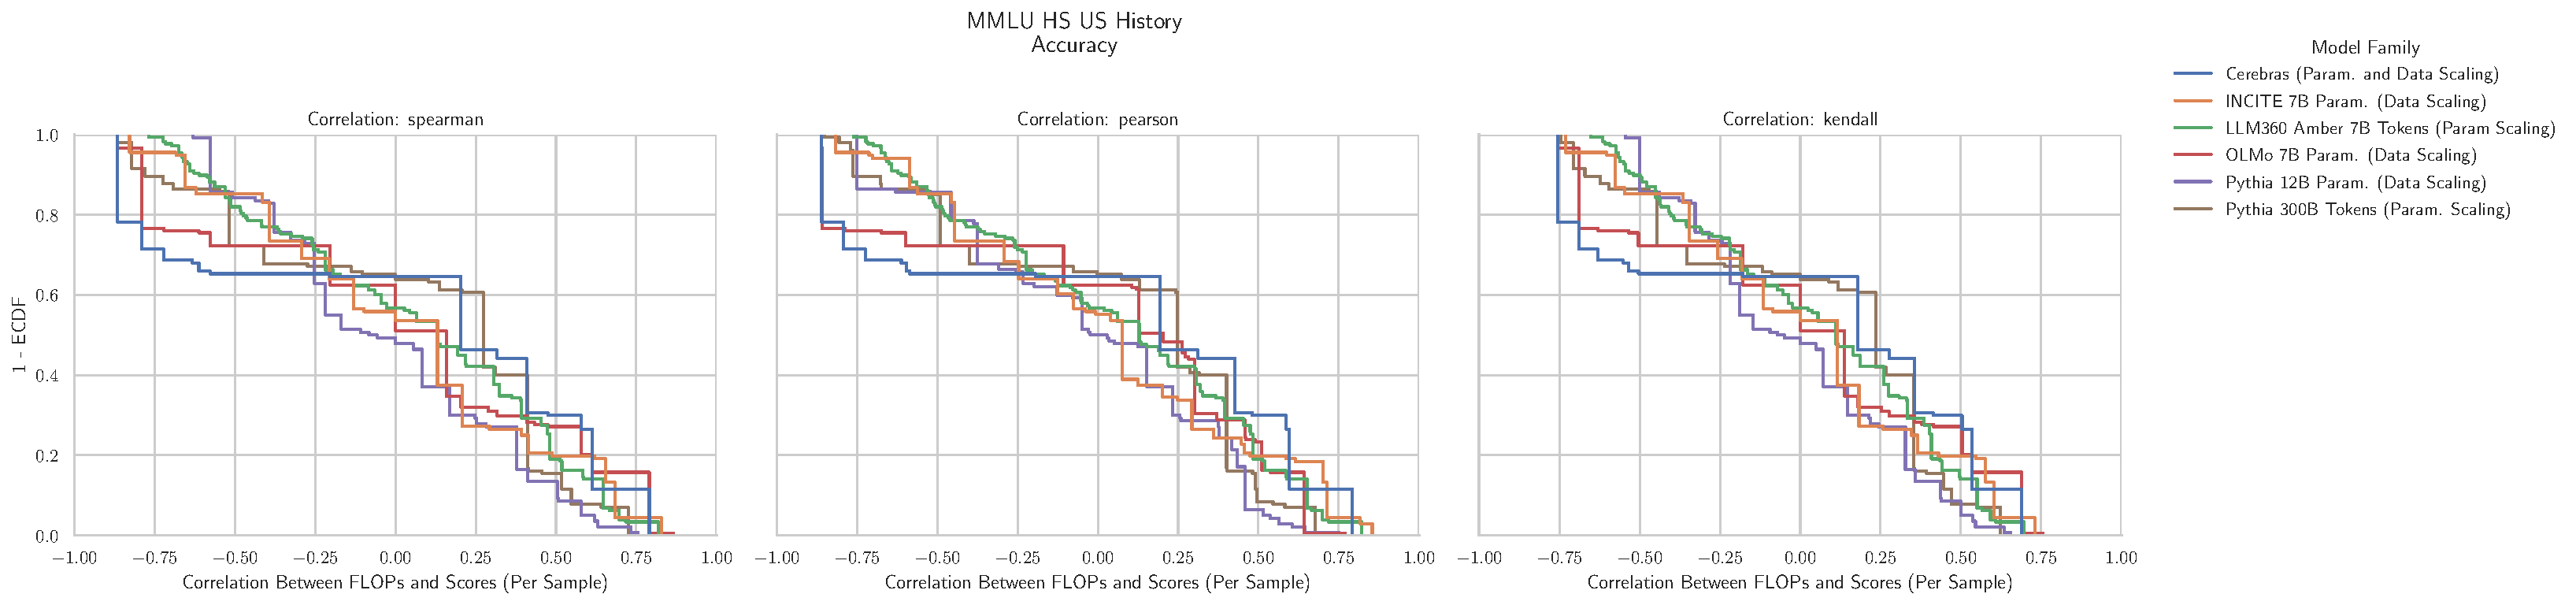
\includegraphics[width=\textwidth]{figures/correlations_between_scores_and_compute/correlation_distributions/mmlu_high_school_us_history/mmlu_high_school_us_history_acc_ecdf_vs_correlation_score_by_modelfamily_split_correlation_metric.pdf}
    \caption{\textbf{MMLU High School US History: Downstream performance is computed via a sequence of transformations that deteriorate correlations between scores and pretraining compute.}}
    \label{app:fig:compute_score_distribution_mmlu_high_school_us_history}
\end{figure}


\clearpage
\subsection{NLP Benchmark: MMLU High School World History \cite{hendrycks2020mmlu}}

\begin{figure}[h!]
    \centering
    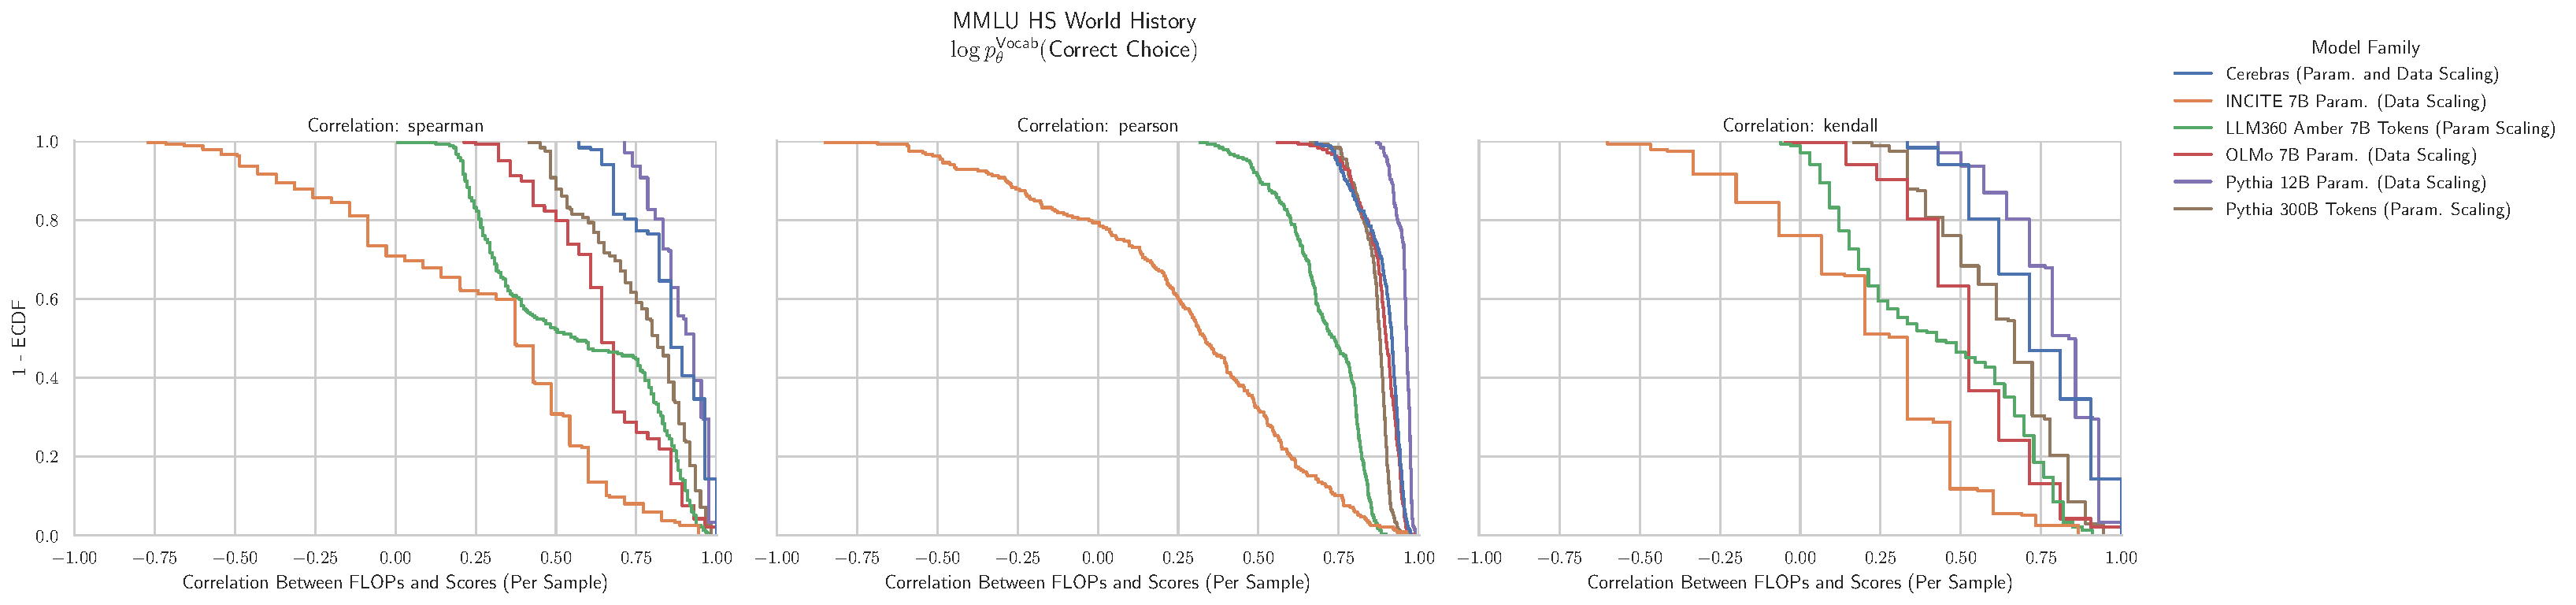
\includegraphics[width=\textwidth]{figures/correlations_between_scores_and_compute/correlation_distributions/mmlu_high_school_world_history/mmlu_high_school_world_history_log_likelihood_correct_ecdf_vs_correlation_score_by_modelfamily_split_correlation_metric.pdf}
    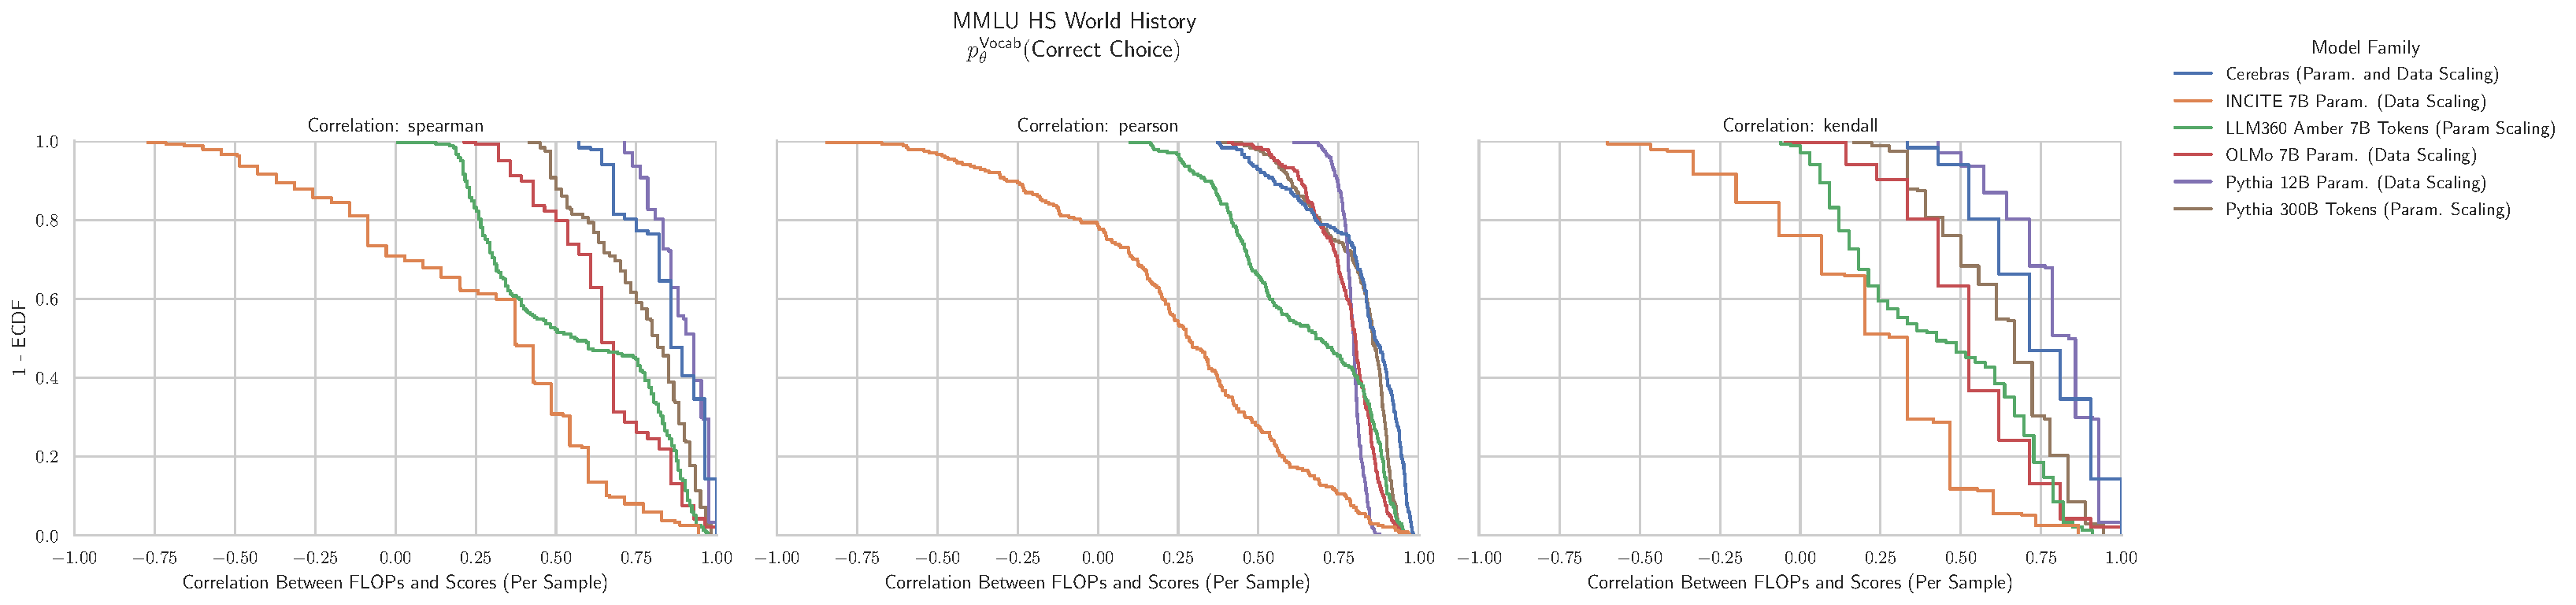
\includegraphics[width=\textwidth]{figures/correlations_between_scores_and_compute/correlation_distributions/mmlu_high_school_world_history/mmlu_high_school_world_history_prob_correct_vocab_ecdf_vs_correlation_score_by_modelfamily_split_correlation_metric.pdf}
    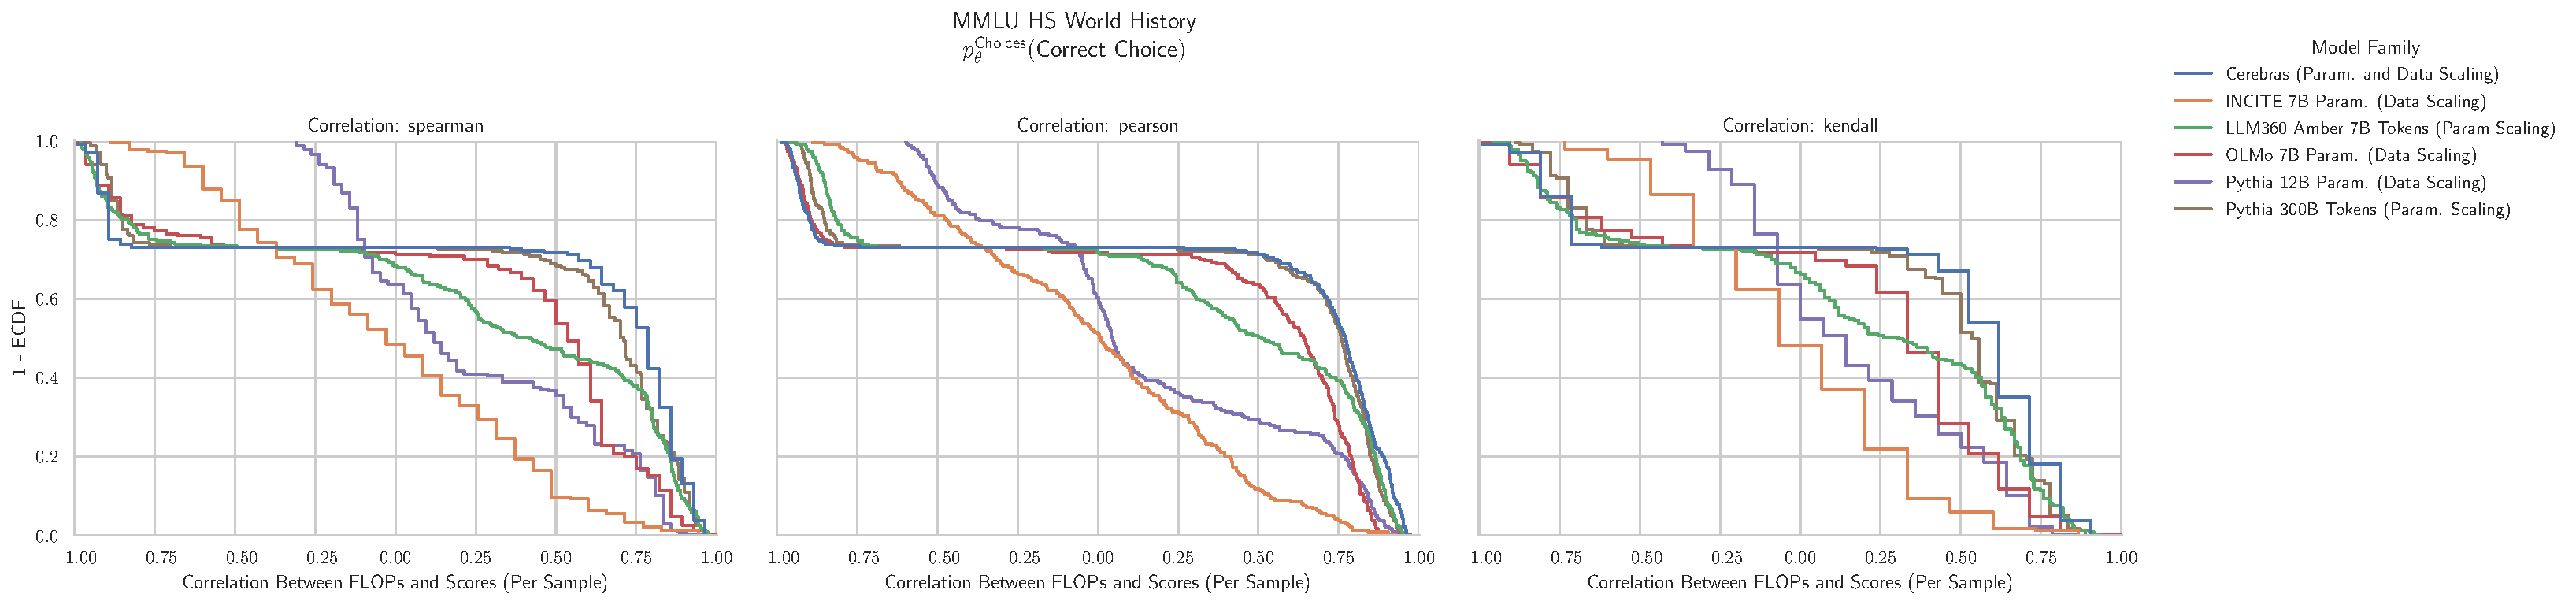
\includegraphics[width=\textwidth]{figures/correlations_between_scores_and_compute/correlation_distributions/mmlu_high_school_world_history/mmlu_high_school_world_history_prob_correct_choices_ecdf_vs_correlation_score_by_modelfamily_split_correlation_metric.pdf}
    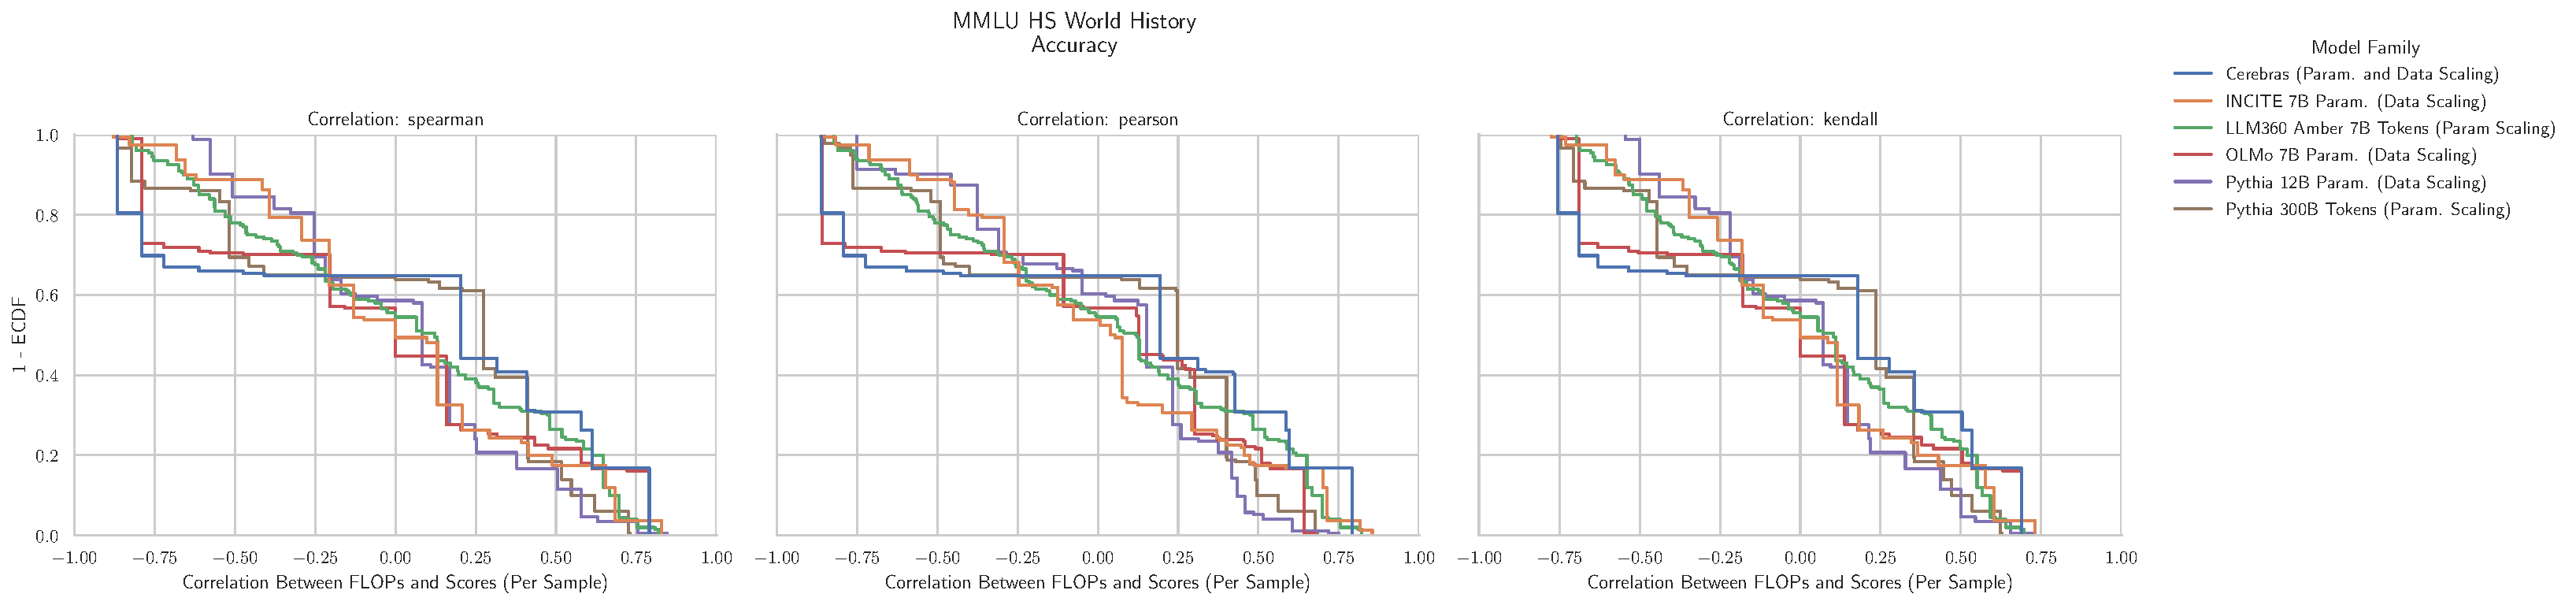
\includegraphics[width=\textwidth]{figures/correlations_between_scores_and_compute/correlation_distributions/mmlu_high_school_world_history/mmlu_high_school_world_history_acc_ecdf_vs_correlation_score_by_modelfamily_split_correlation_metric.pdf}
    \caption{\textbf{MMLU High School World History: Downstream performance is computed via a sequence of transformations that deteriorate correlations between scores and pretraining compute.}}
    \label{app:fig:compute_score_distribution_mmlu_high_school_world_history}
\end{figure}


\clearpage
\subsection{NLP Benchmark: MMLU Human Aging \cite{hendrycks2020mmlu}}

\begin{figure}[h!]
    \centering
    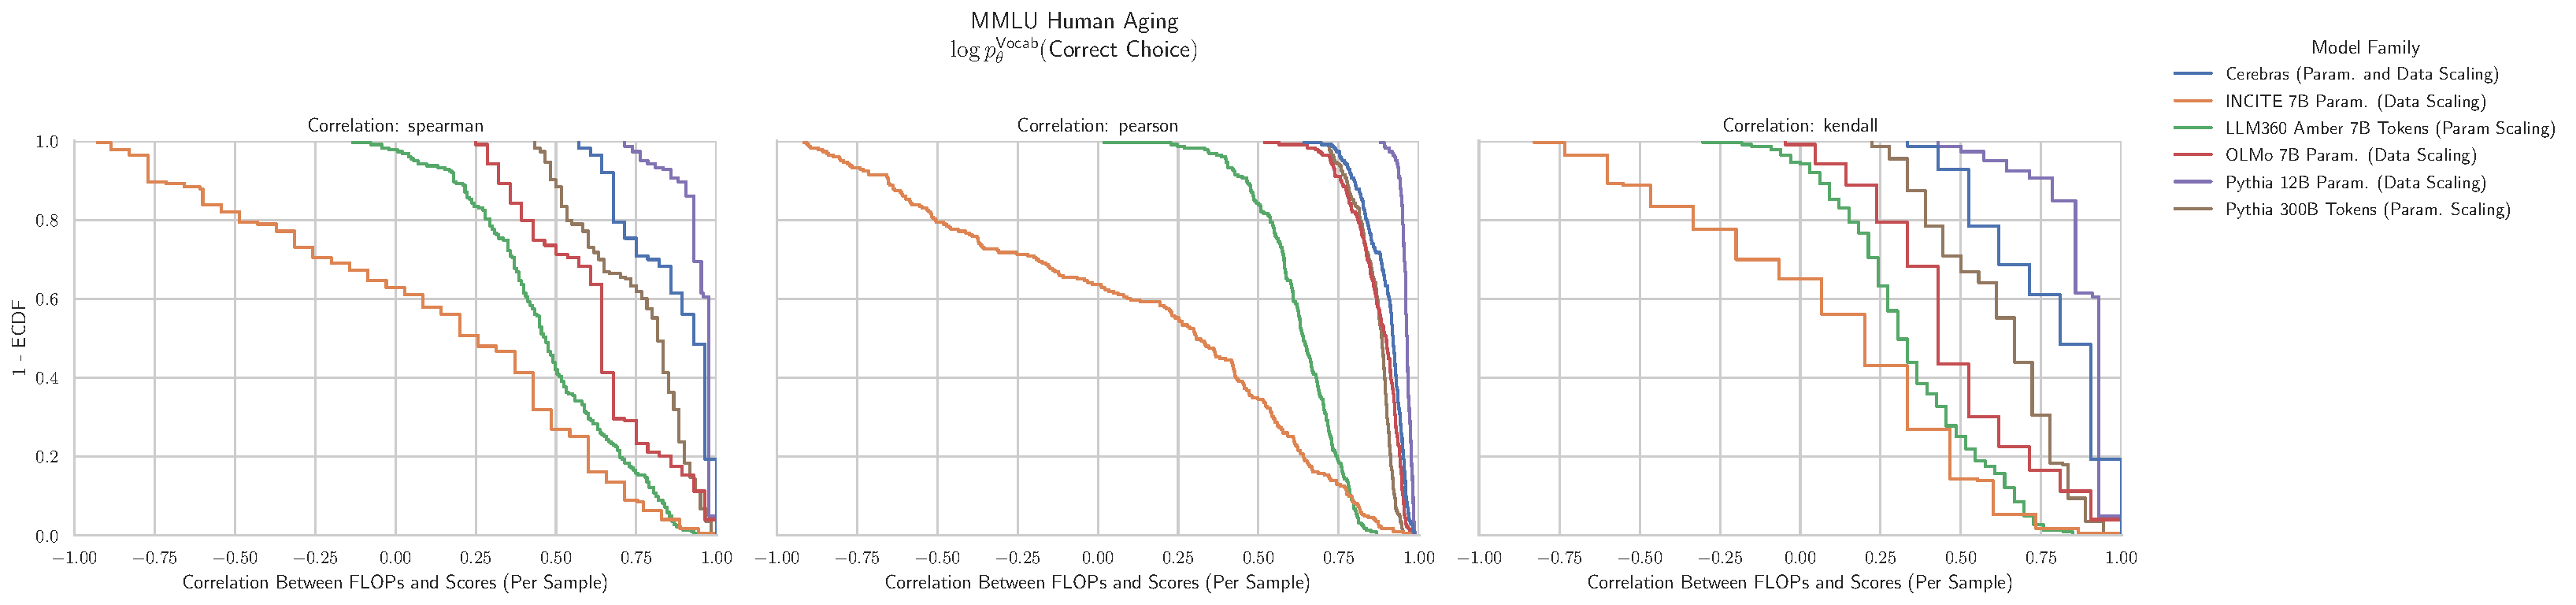
\includegraphics[width=\textwidth]{figures/correlations_between_scores_and_compute/correlation_distributions/mmlu_human_aging/mmlu_human_aging_log_likelihood_correct_ecdf_vs_correlation_score_by_modelfamily_split_correlation_metric.pdf}
    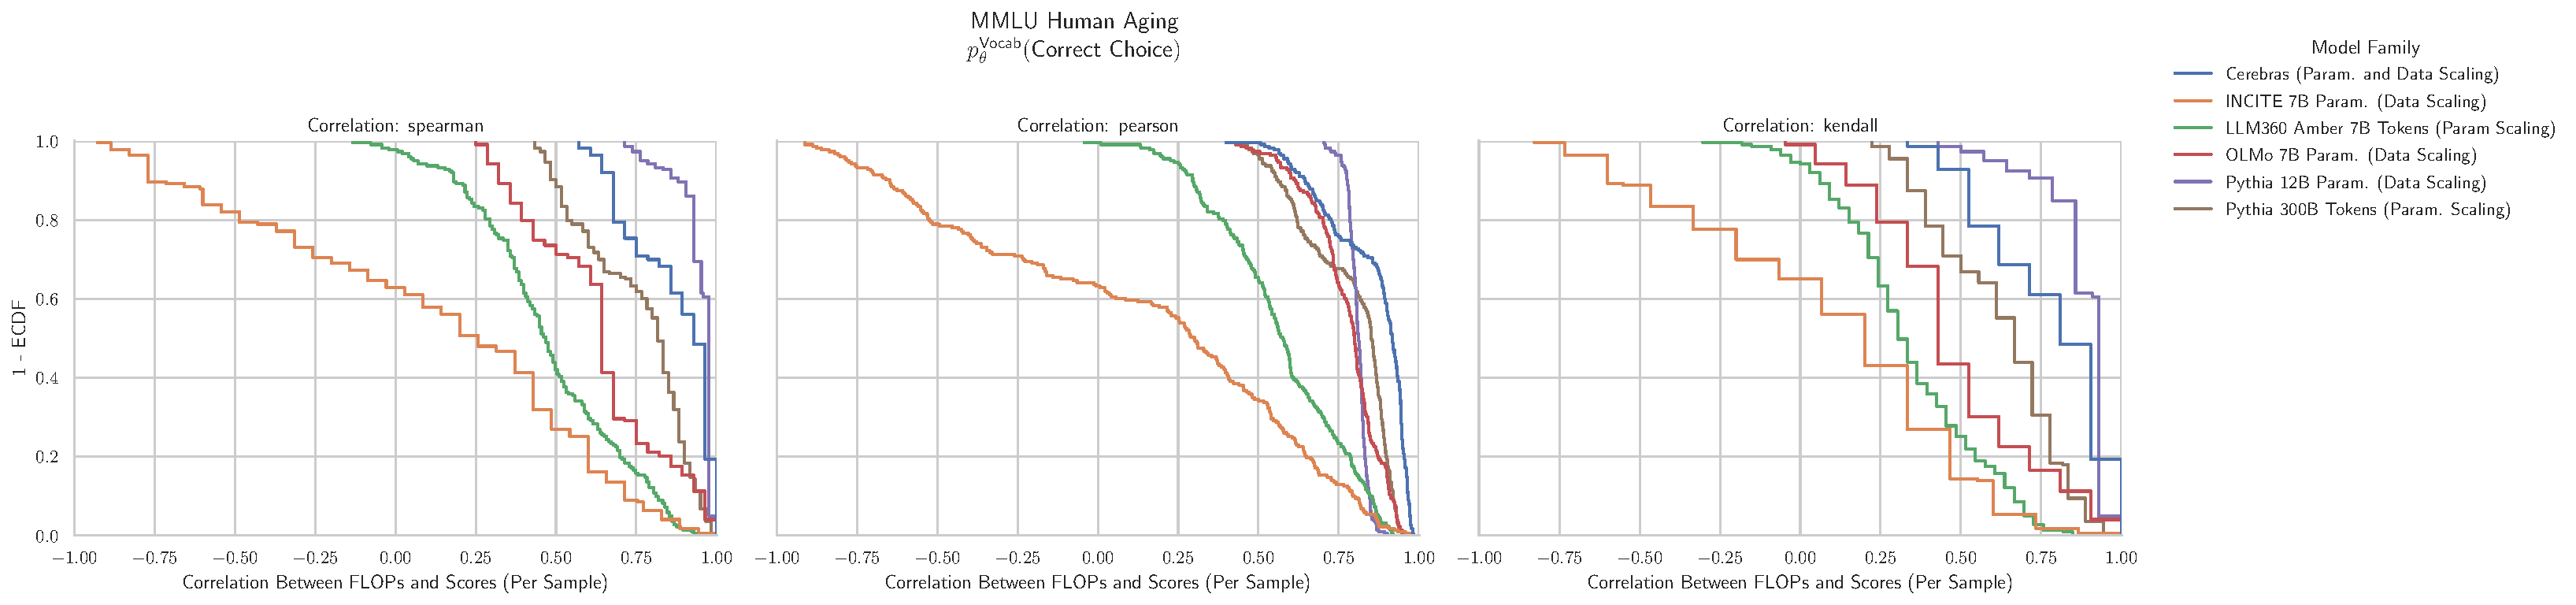
\includegraphics[width=\textwidth]{figures/correlations_between_scores_and_compute/correlation_distributions/mmlu_human_aging/mmlu_human_aging_prob_correct_vocab_ecdf_vs_correlation_score_by_modelfamily_split_correlation_metric.pdf}
    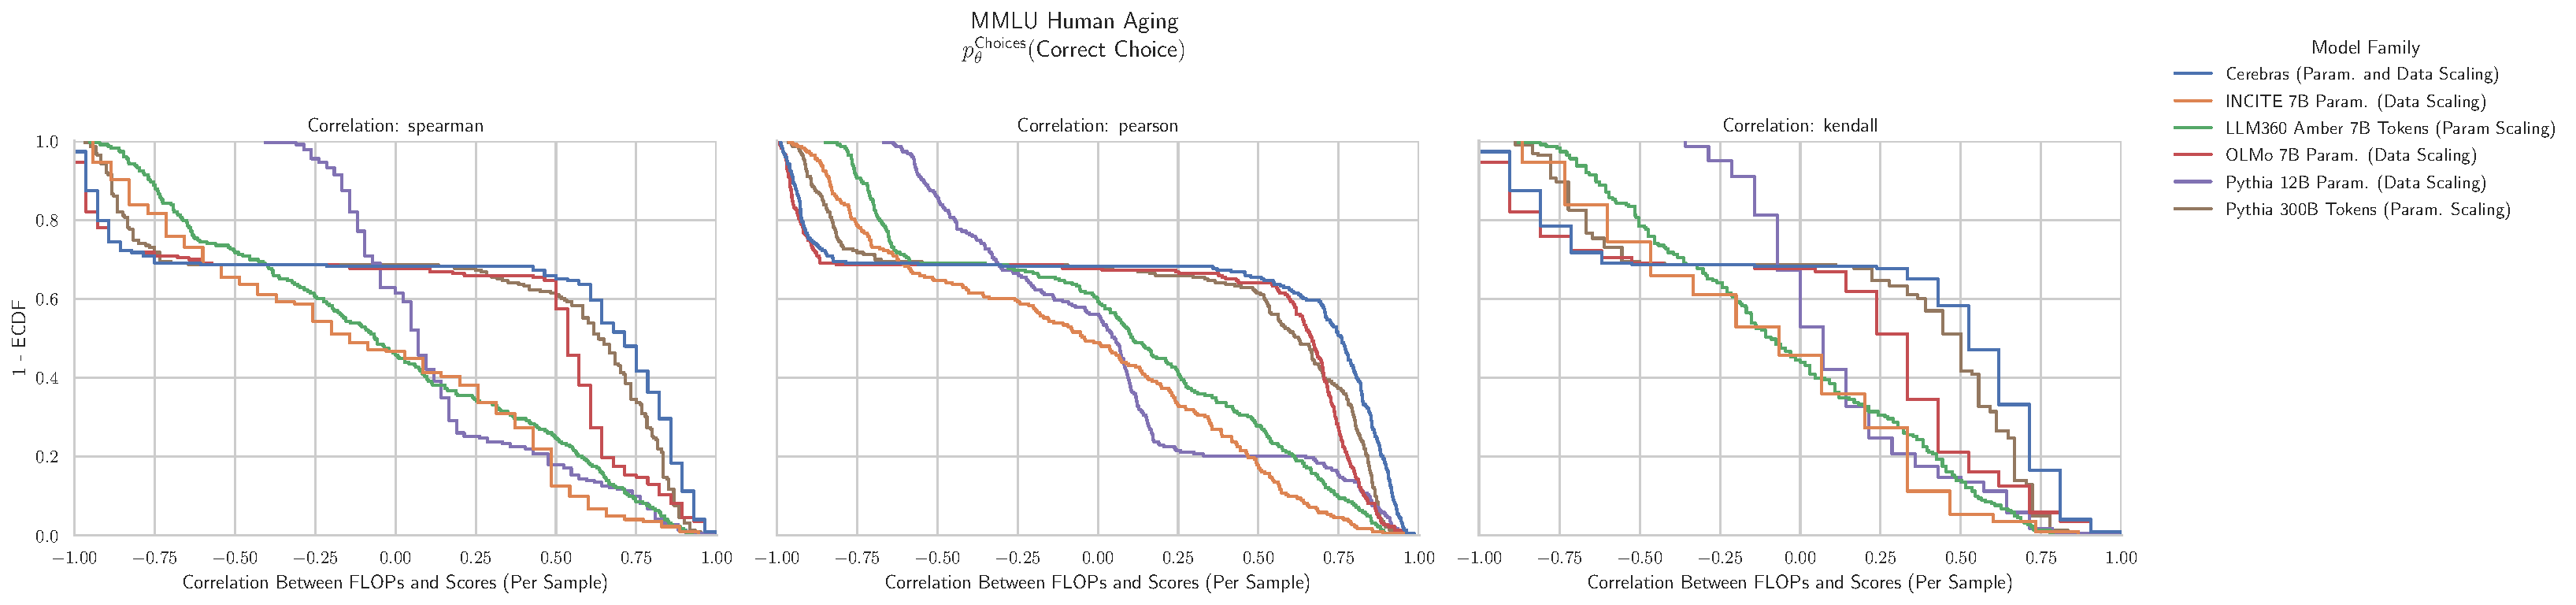
\includegraphics[width=\textwidth]{figures/correlations_between_scores_and_compute/correlation_distributions/mmlu_human_aging/mmlu_human_aging_prob_correct_choices_ecdf_vs_correlation_score_by_modelfamily_split_correlation_metric.pdf}
    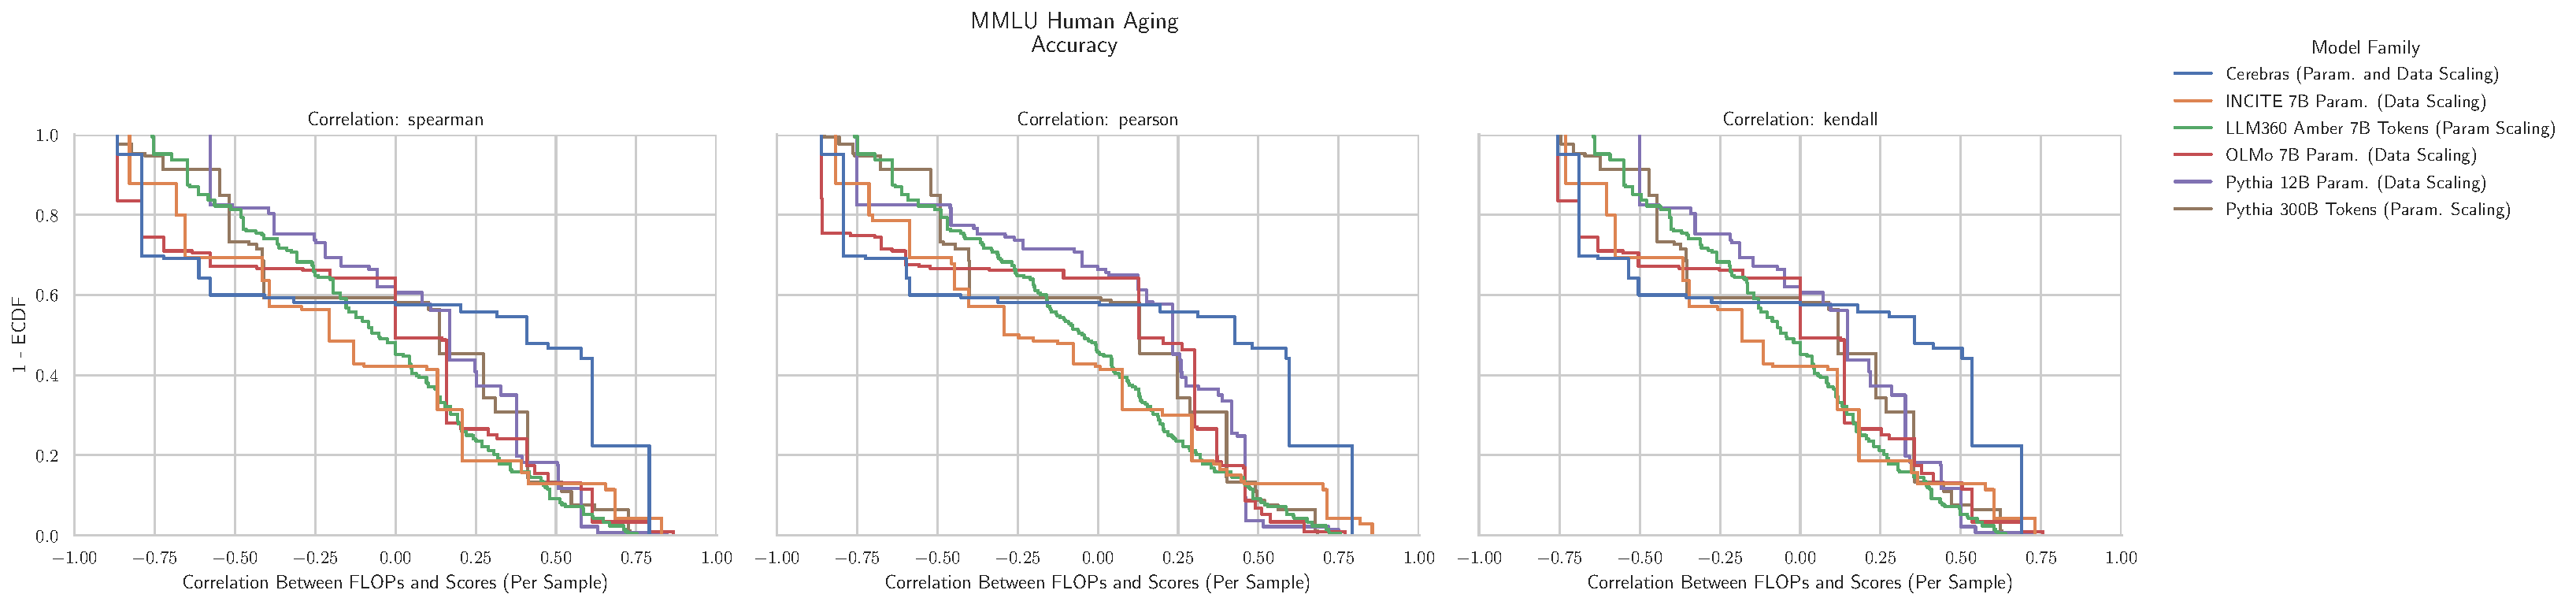
\includegraphics[width=\textwidth]{figures/correlations_between_scores_and_compute/correlation_distributions/mmlu_human_aging/mmlu_human_aging_acc_ecdf_vs_correlation_score_by_modelfamily_split_correlation_metric.pdf}
    \caption{\textbf{MMLU Human Aging: Downstream performance is computed via a sequence of transformations that deteriorate correlations between scores and pretraining compute.}}
    \label{app:fig:compute_score_distribution_mmlu_human_aging}
\end{figure}


\clearpage
\subsection{NLP Benchmark: MMLU Human Sexuality \cite{hendrycks2020mmlu}}

\begin{figure}[h!]
    \centering
    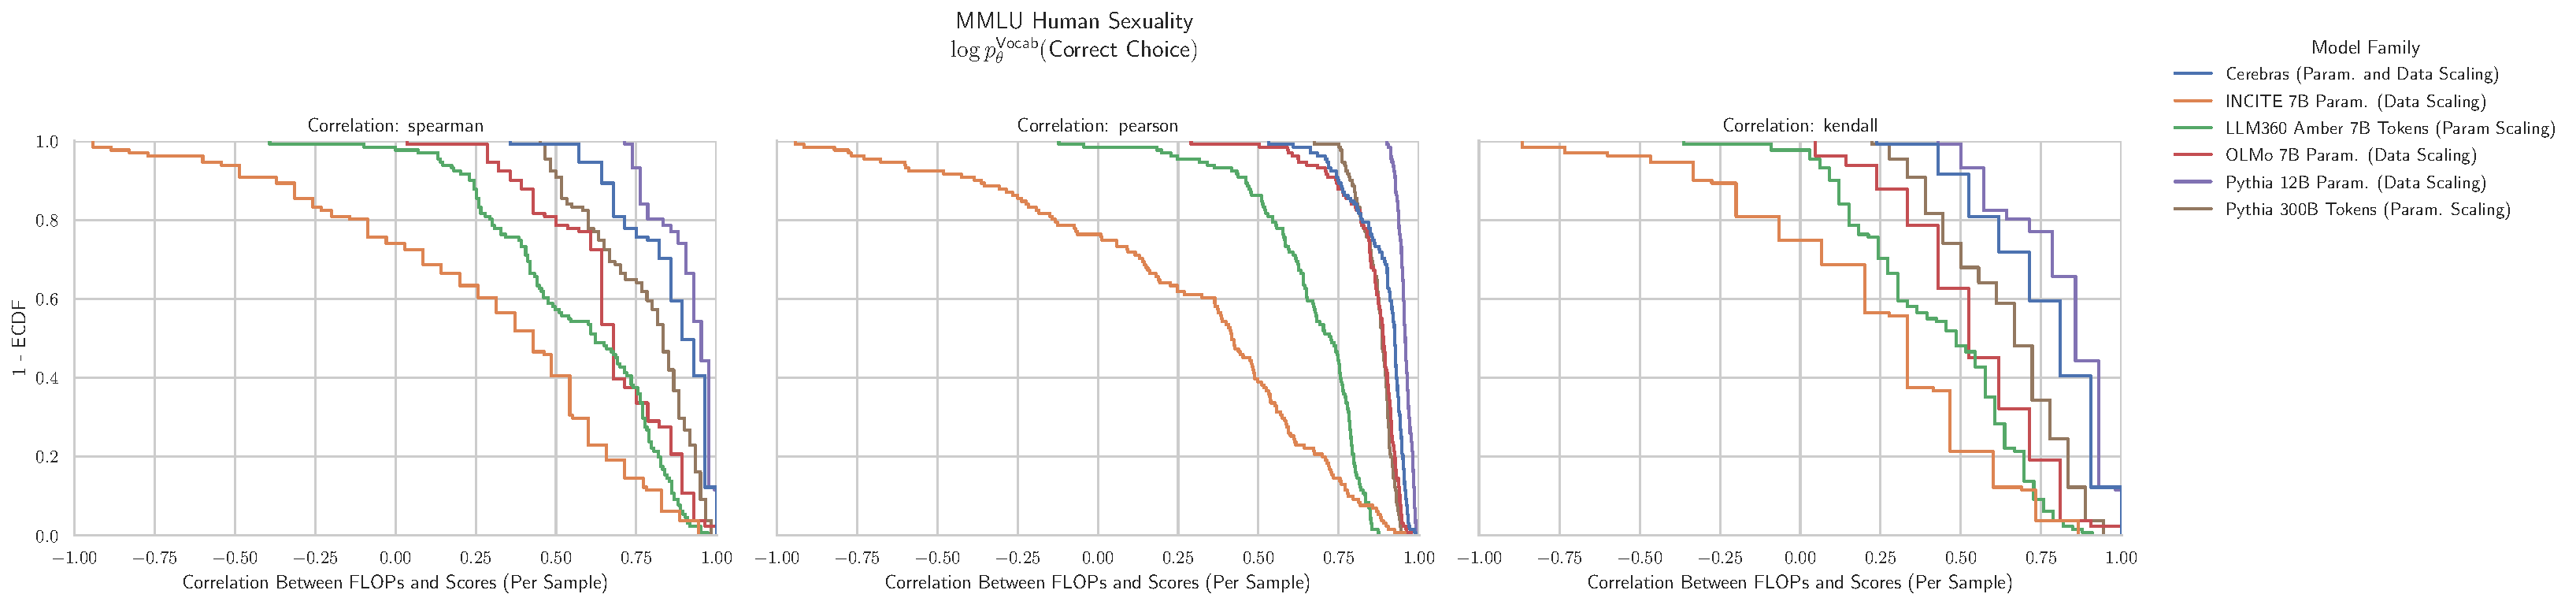
\includegraphics[width=\textwidth]{figures/correlations_between_scores_and_compute/correlation_distributions/mmlu_human_sexuality/mmlu_human_sexuality_log_likelihood_correct_ecdf_vs_correlation_score_by_modelfamily_split_correlation_metric.pdf}
    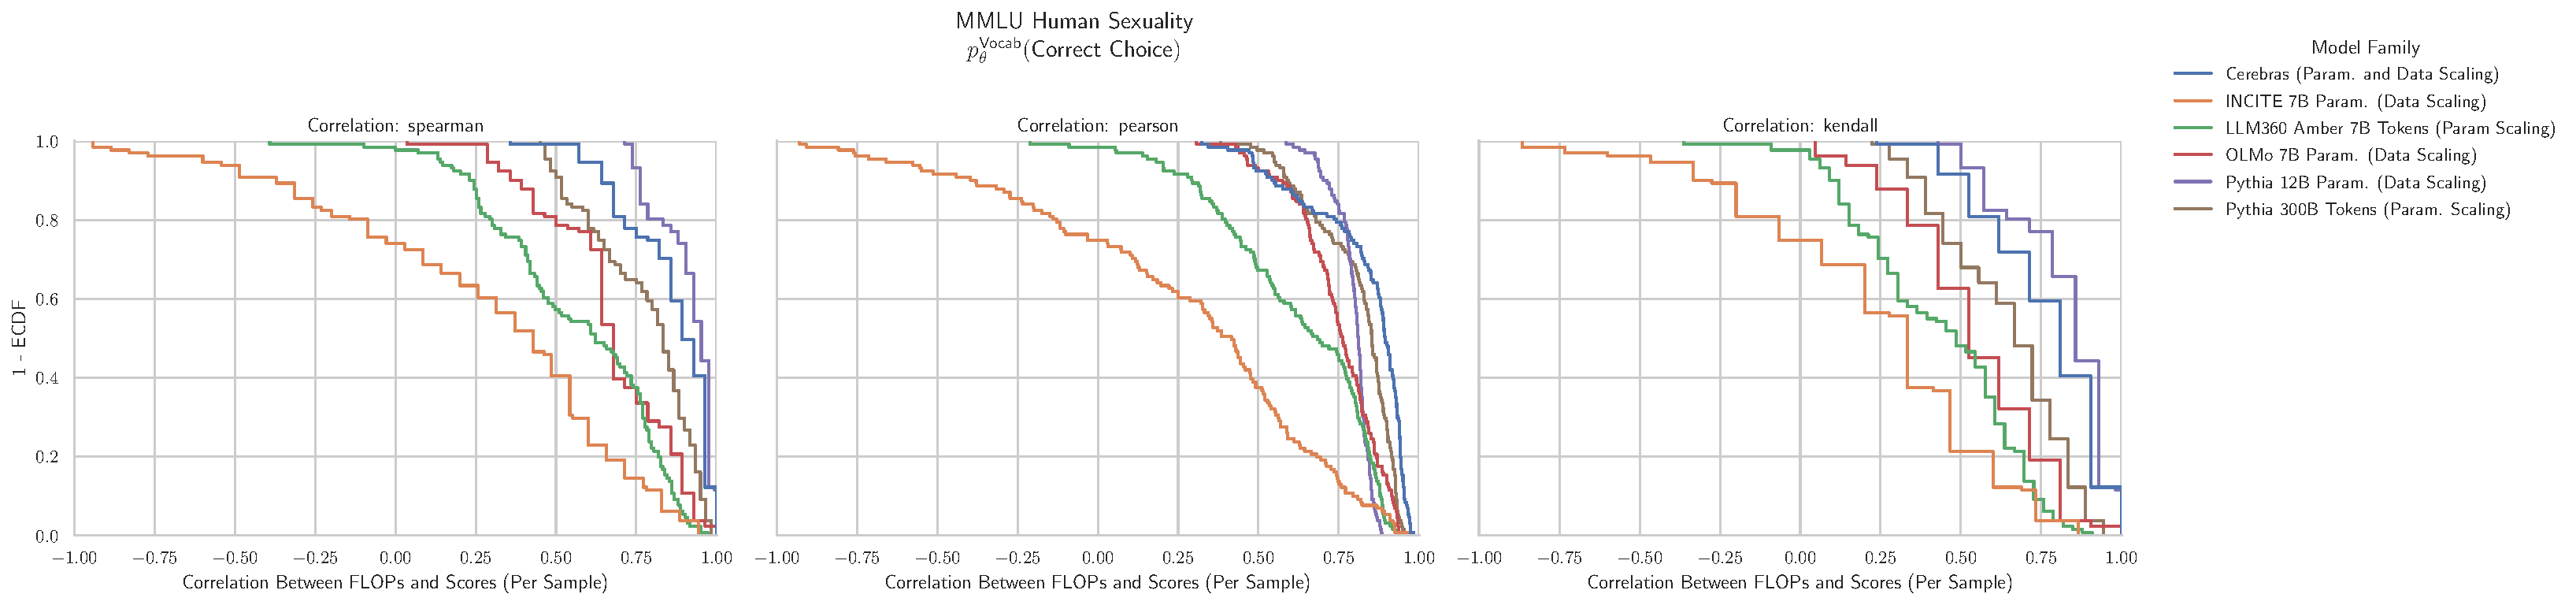
\includegraphics[width=\textwidth]{figures/correlations_between_scores_and_compute/correlation_distributions/mmlu_human_sexuality/mmlu_human_sexuality_prob_correct_vocab_ecdf_vs_correlation_score_by_modelfamily_split_correlation_metric.pdf}
    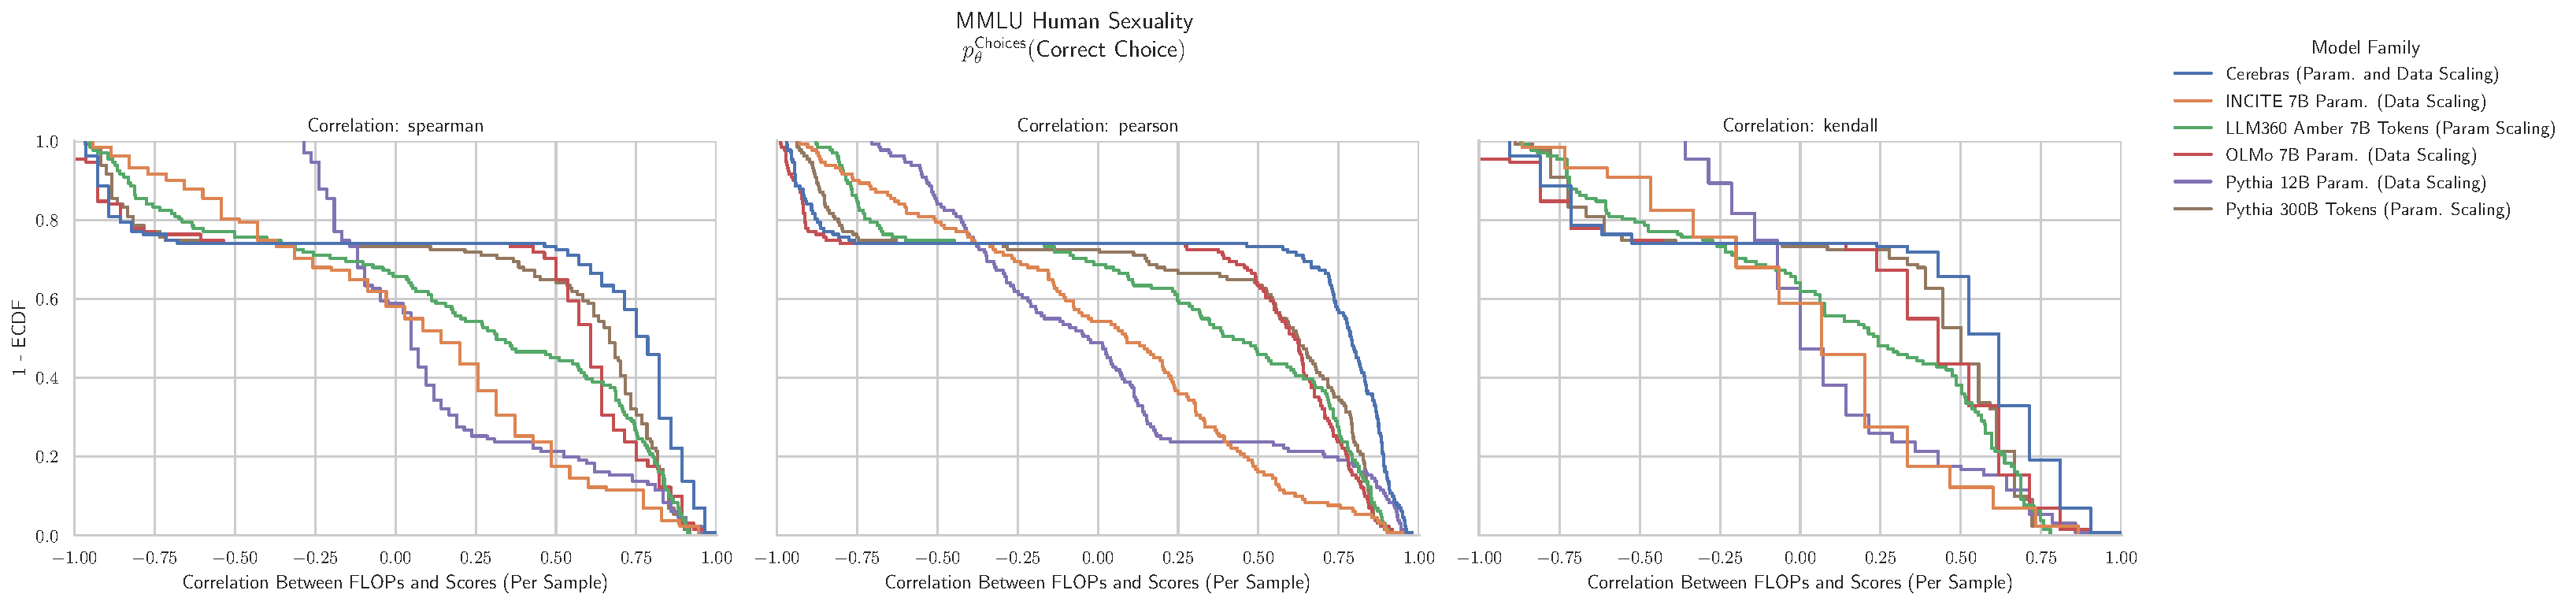
\includegraphics[width=\textwidth]{figures/correlations_between_scores_and_compute/correlation_distributions/mmlu_human_sexuality/mmlu_human_sexuality_prob_correct_choices_ecdf_vs_correlation_score_by_modelfamily_split_correlation_metric.pdf}
    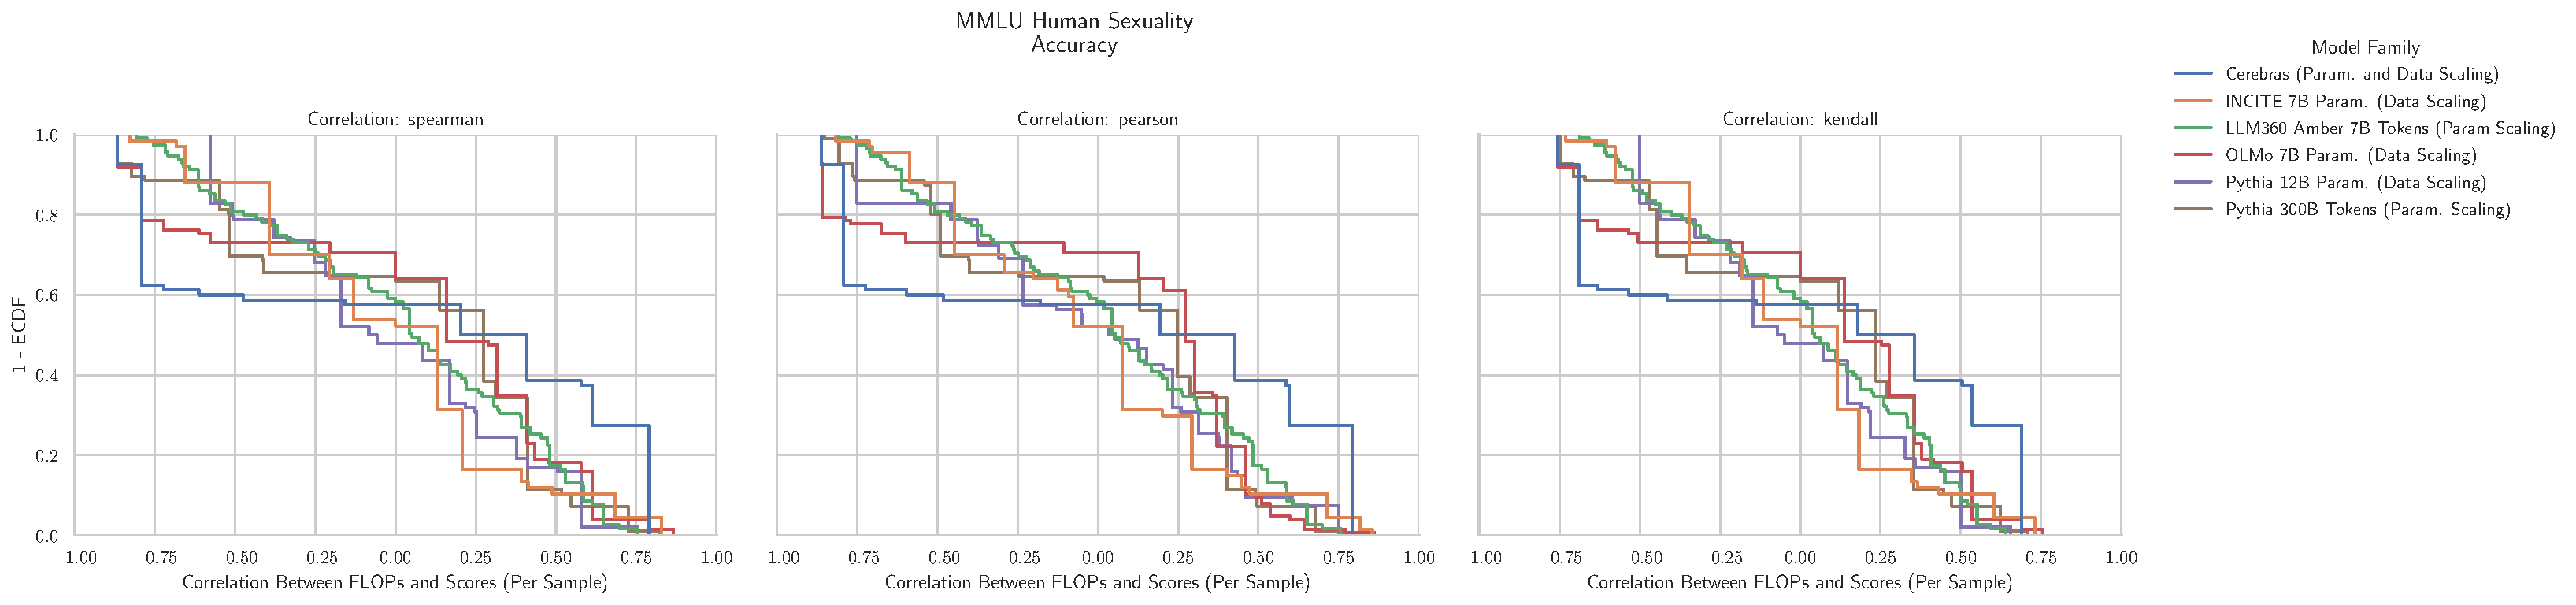
\includegraphics[width=\textwidth]{figures/correlations_between_scores_and_compute/correlation_distributions/mmlu_human_sexuality/mmlu_human_sexuality_acc_ecdf_vs_correlation_score_by_modelfamily_split_correlation_metric.pdf}
    \caption{\textbf{MMLU Human Sexuality: Downstream performance is computed via a sequence of transformations that deteriorate correlations between scores and pretraining compute.}}
    \label{app:fig:compute_score_distribution_mmlu_human_sexuality}
\end{figure}

\clearpage
\subsection{NLP Benchmark: MMLU International Law \cite{hendrycks2020mmlu}}

\begin{figure}[h!]
    \centering
    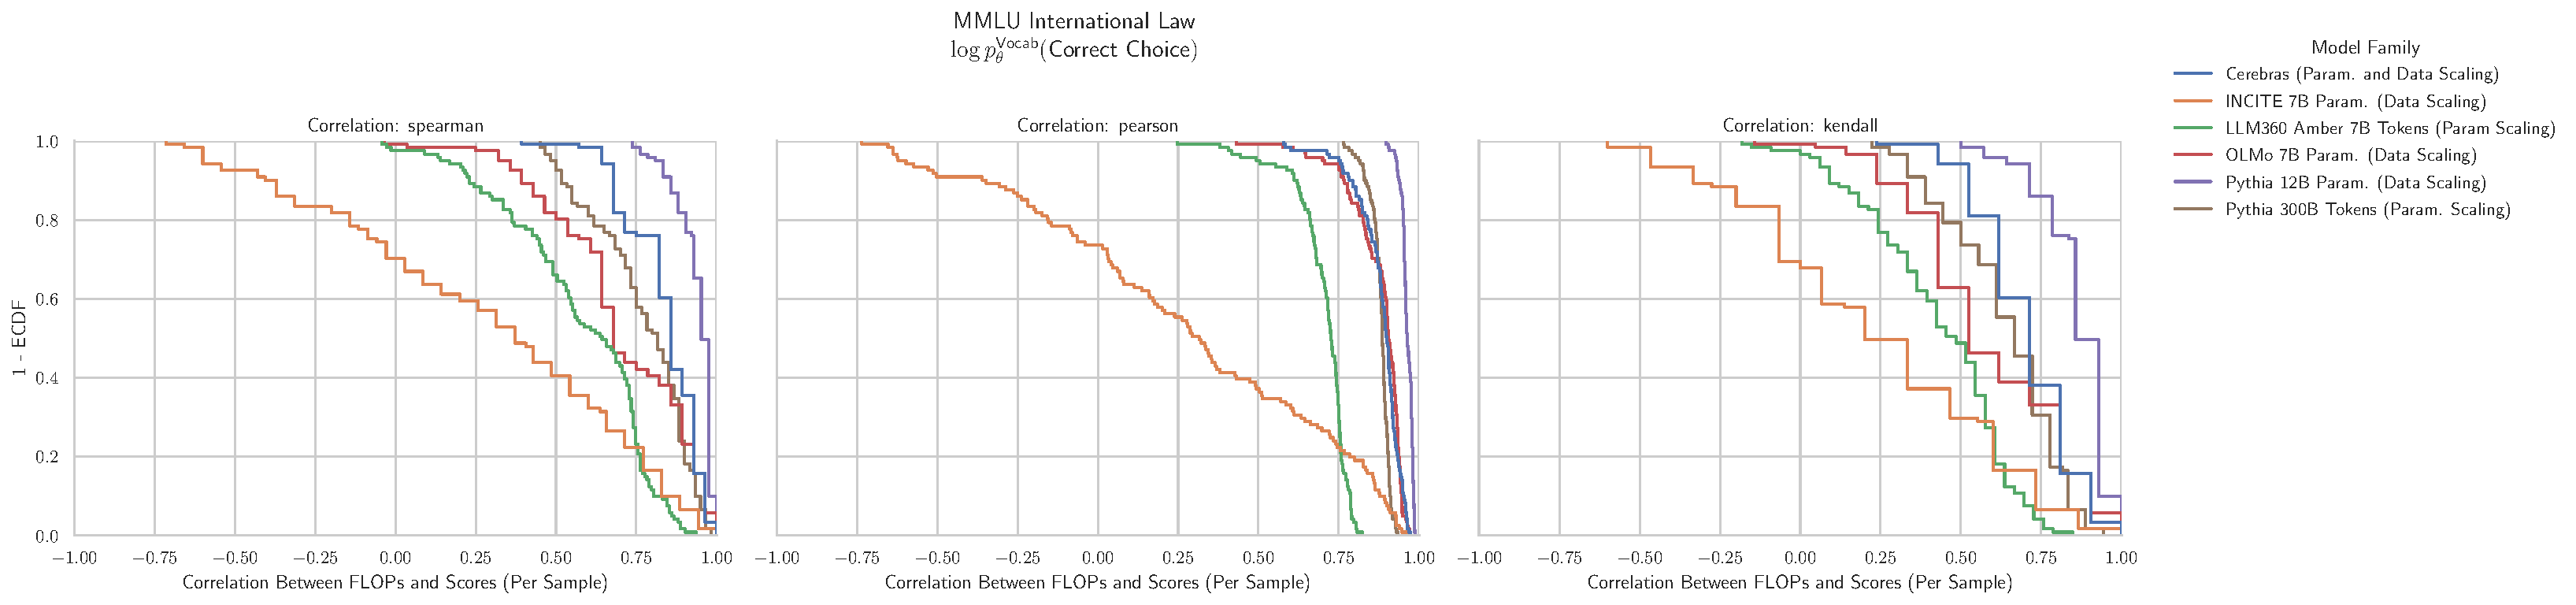
\includegraphics[width=\textwidth]{figures/correlations_between_scores_and_compute/correlation_distributions/mmlu_international_law/mmlu_international_law_log_likelihood_correct_ecdf_vs_correlation_score_by_modelfamily_split_correlation_metric.pdf}
    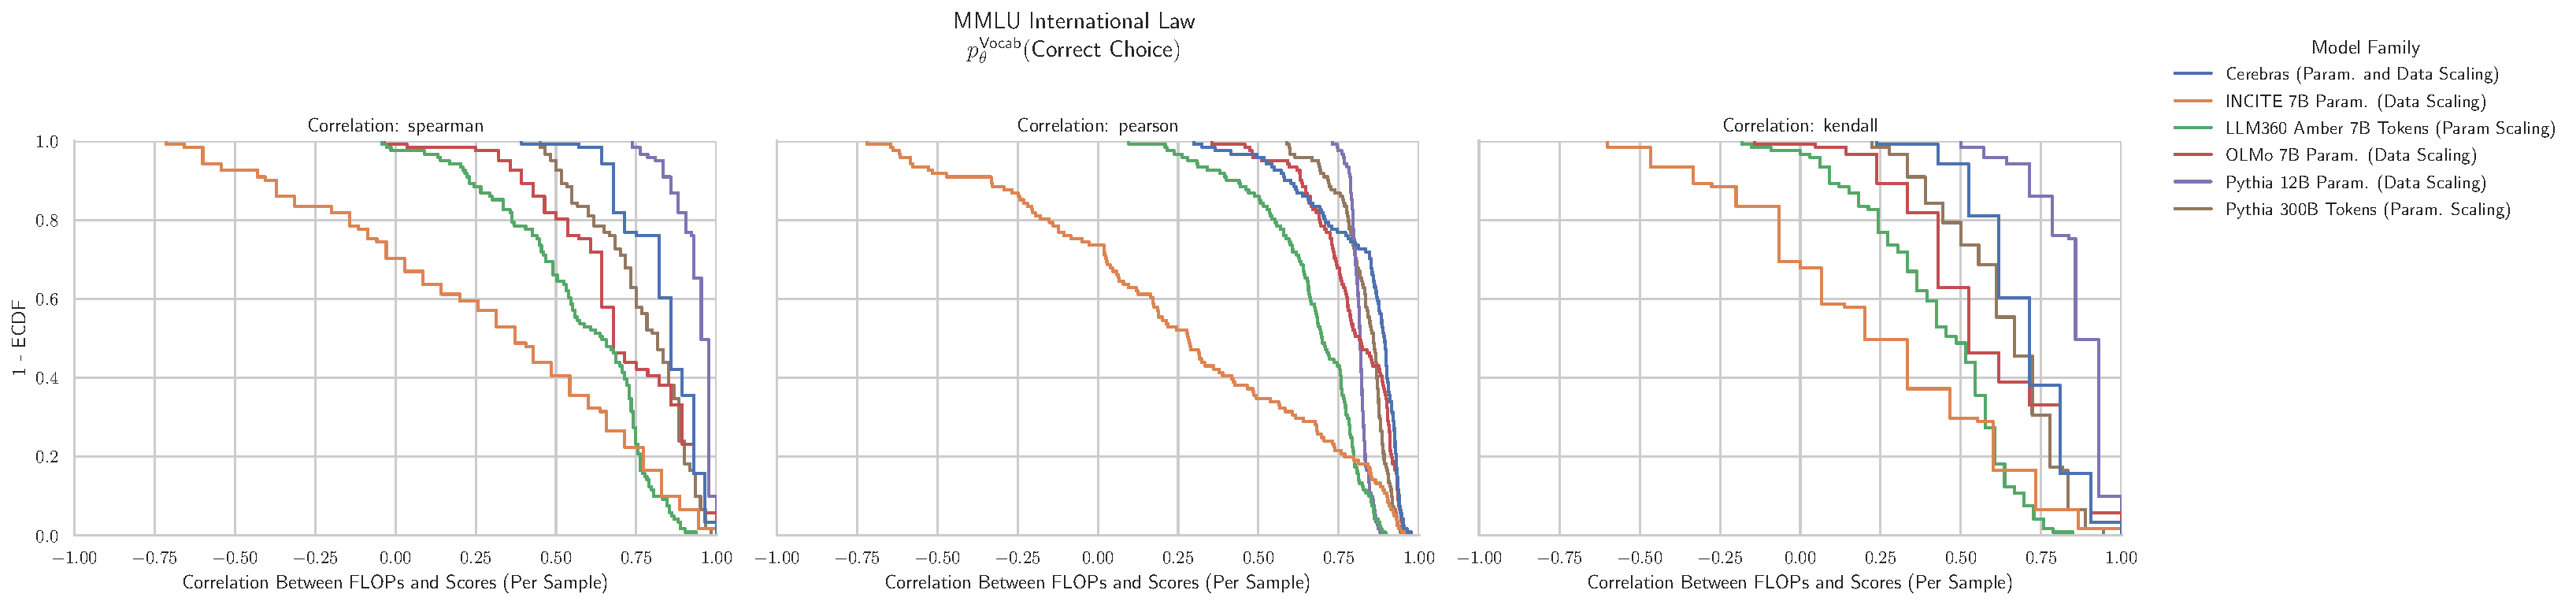
\includegraphics[width=\textwidth]{figures/correlations_between_scores_and_compute/correlation_distributions/mmlu_international_law/mmlu_international_law_prob_correct_vocab_ecdf_vs_correlation_score_by_modelfamily_split_correlation_metric.pdf}
    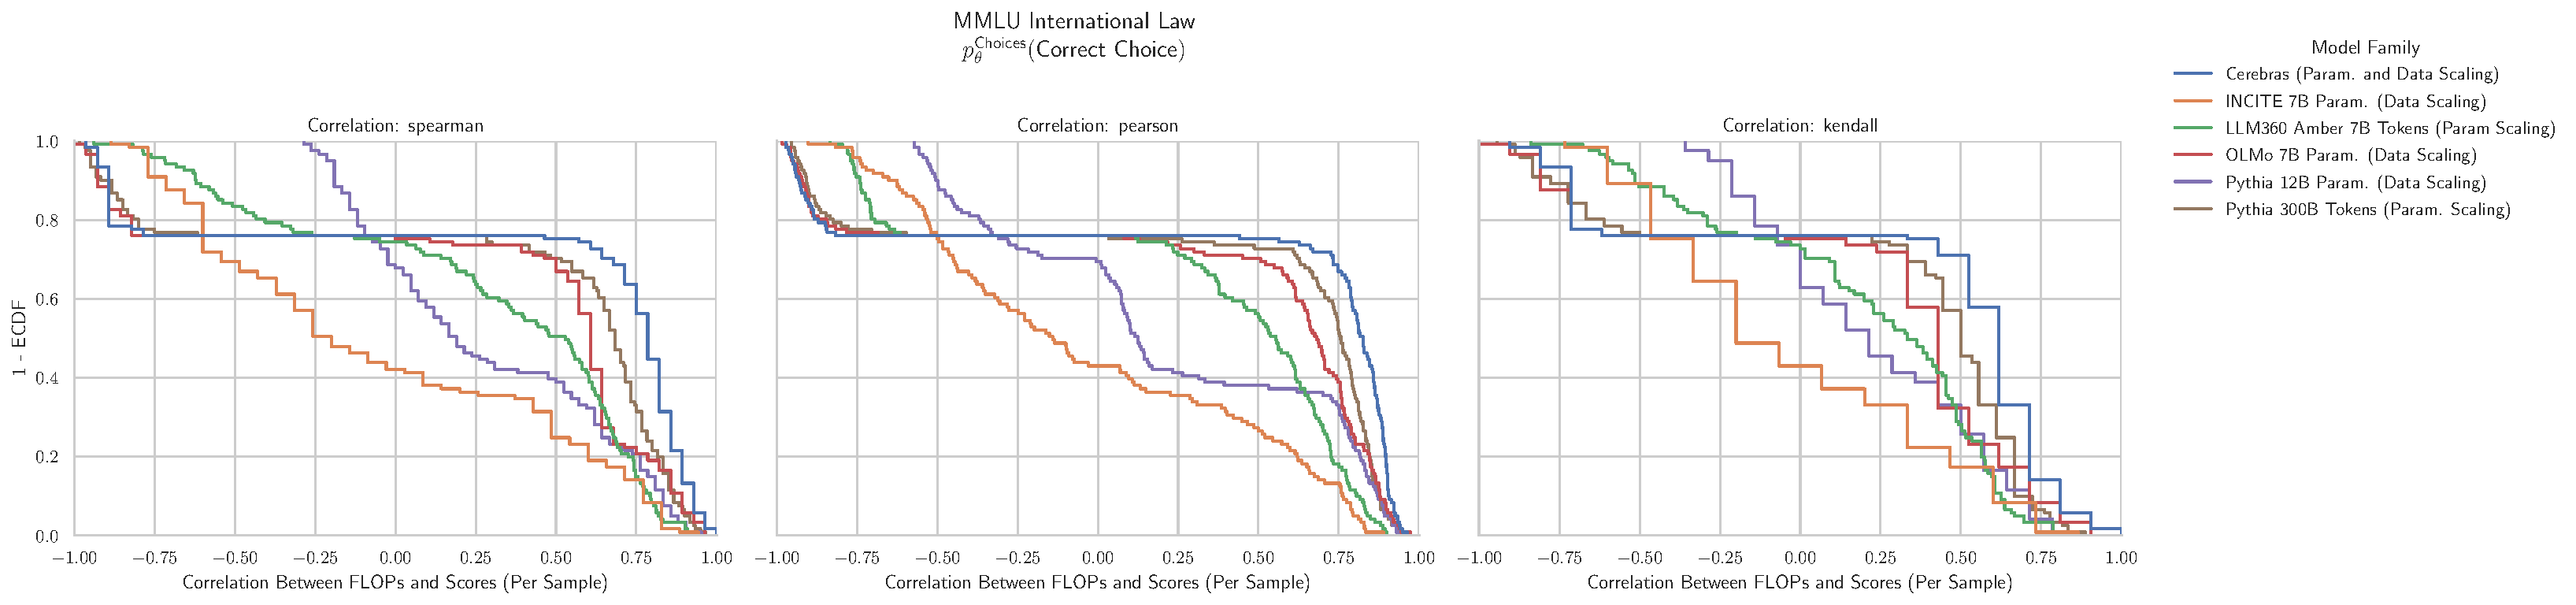
\includegraphics[width=\textwidth]{figures/correlations_between_scores_and_compute/correlation_distributions/mmlu_international_law/mmlu_international_law_prob_correct_choices_ecdf_vs_correlation_score_by_modelfamily_split_correlation_metric.pdf}
    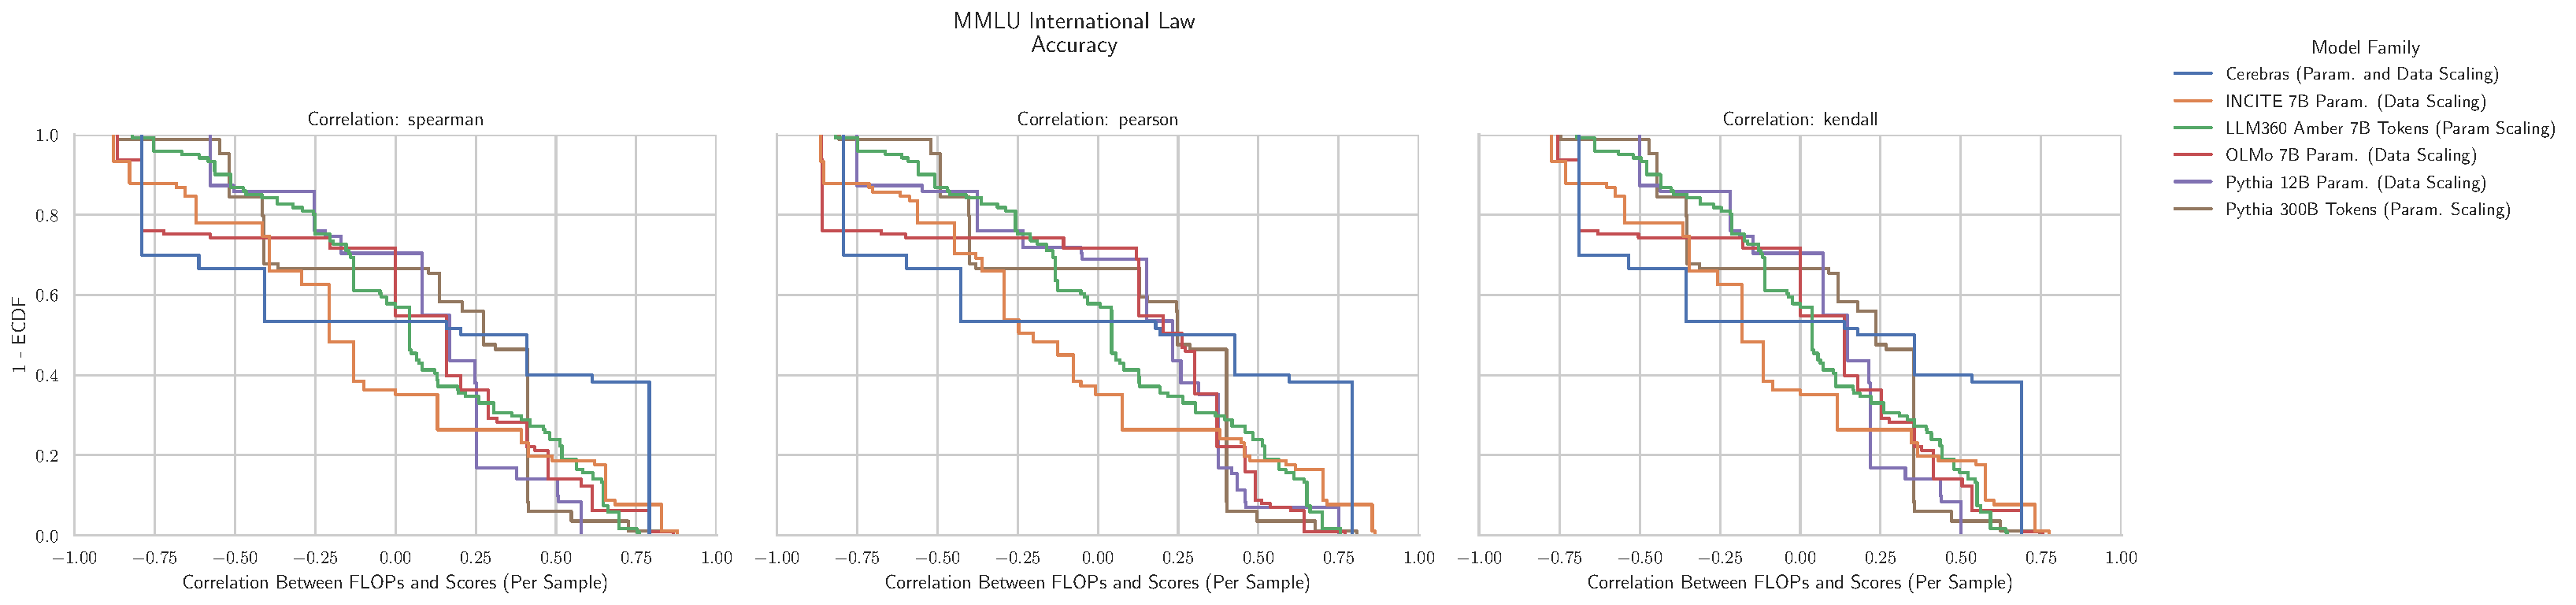
\includegraphics[width=\textwidth]{figures/correlations_between_scores_and_compute/correlation_distributions/mmlu_international_law/mmlu_international_law_acc_ecdf_vs_correlation_score_by_modelfamily_split_correlation_metric.pdf}
    \caption{\textbf{MMLU International Law: Downstream performance is computed via a sequence of transformations that deteriorate correlations between scores and pretraining compute.}}
    \label{app:fig:compute_score_distribution_mmlu_international_law}
\end{figure}


\clearpage
\subsection{NLP Benchmark: MMLU Jurisprudence \cite{hendrycks2020mmlu}}

\begin{figure}[h!]
    \centering
    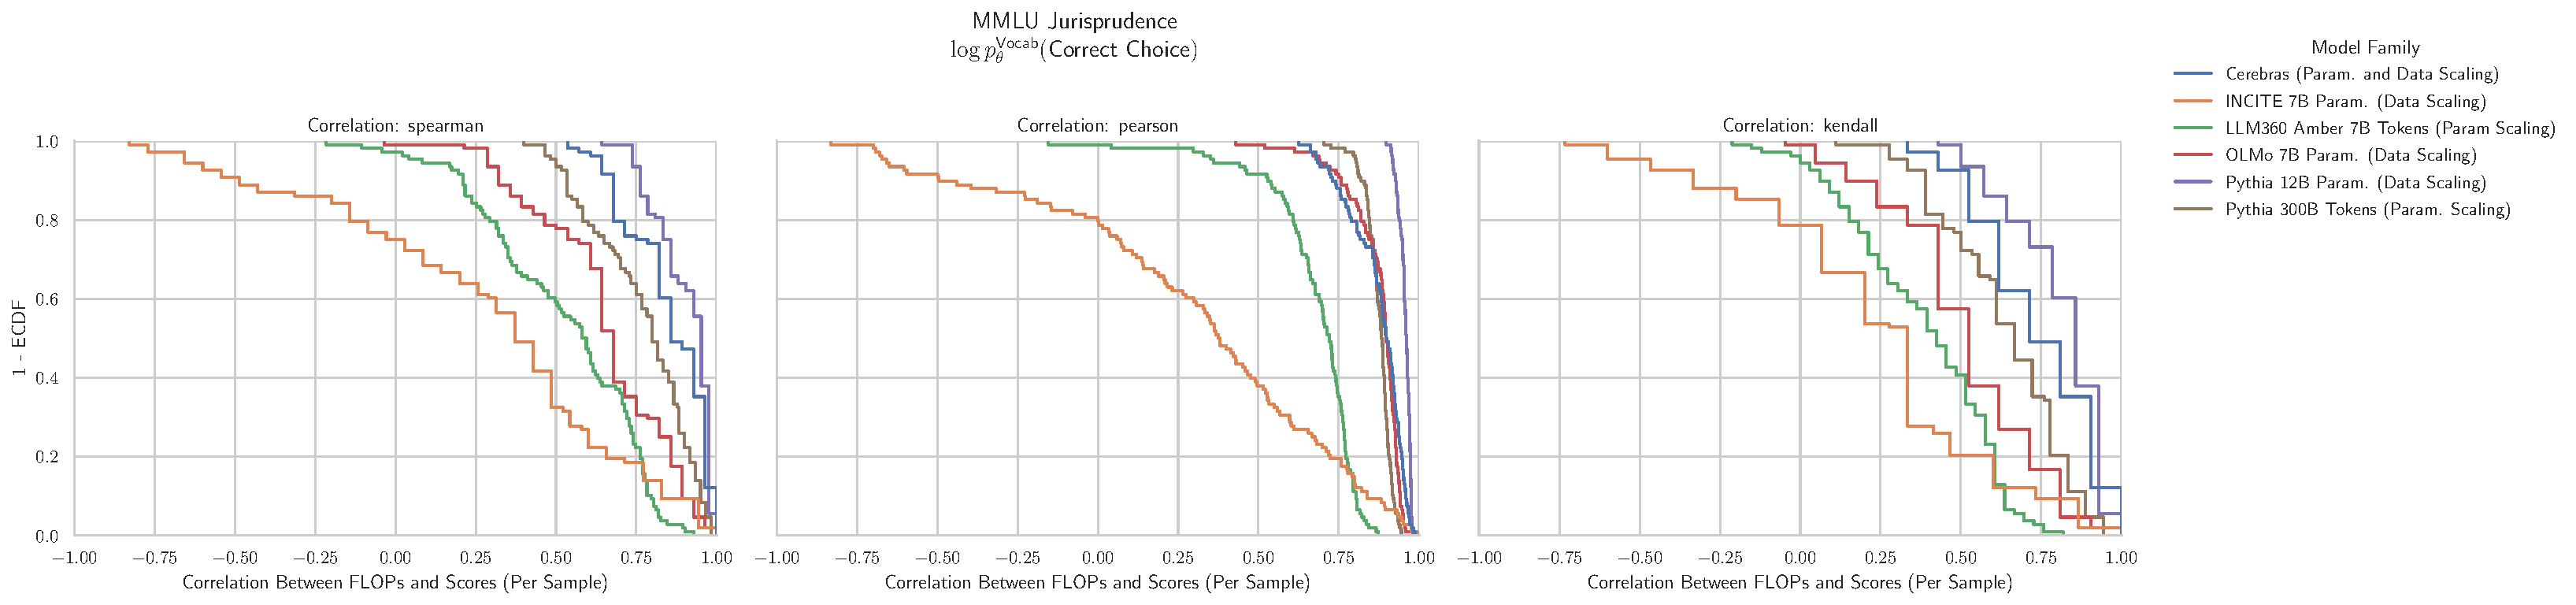
\includegraphics[width=\textwidth]{figures/correlations_between_scores_and_compute/correlation_distributions/mmlu_jurisprudence/mmlu_jurisprudence_log_likelihood_correct_ecdf_vs_correlation_score_by_modelfamily_split_correlation_metric.pdf}
    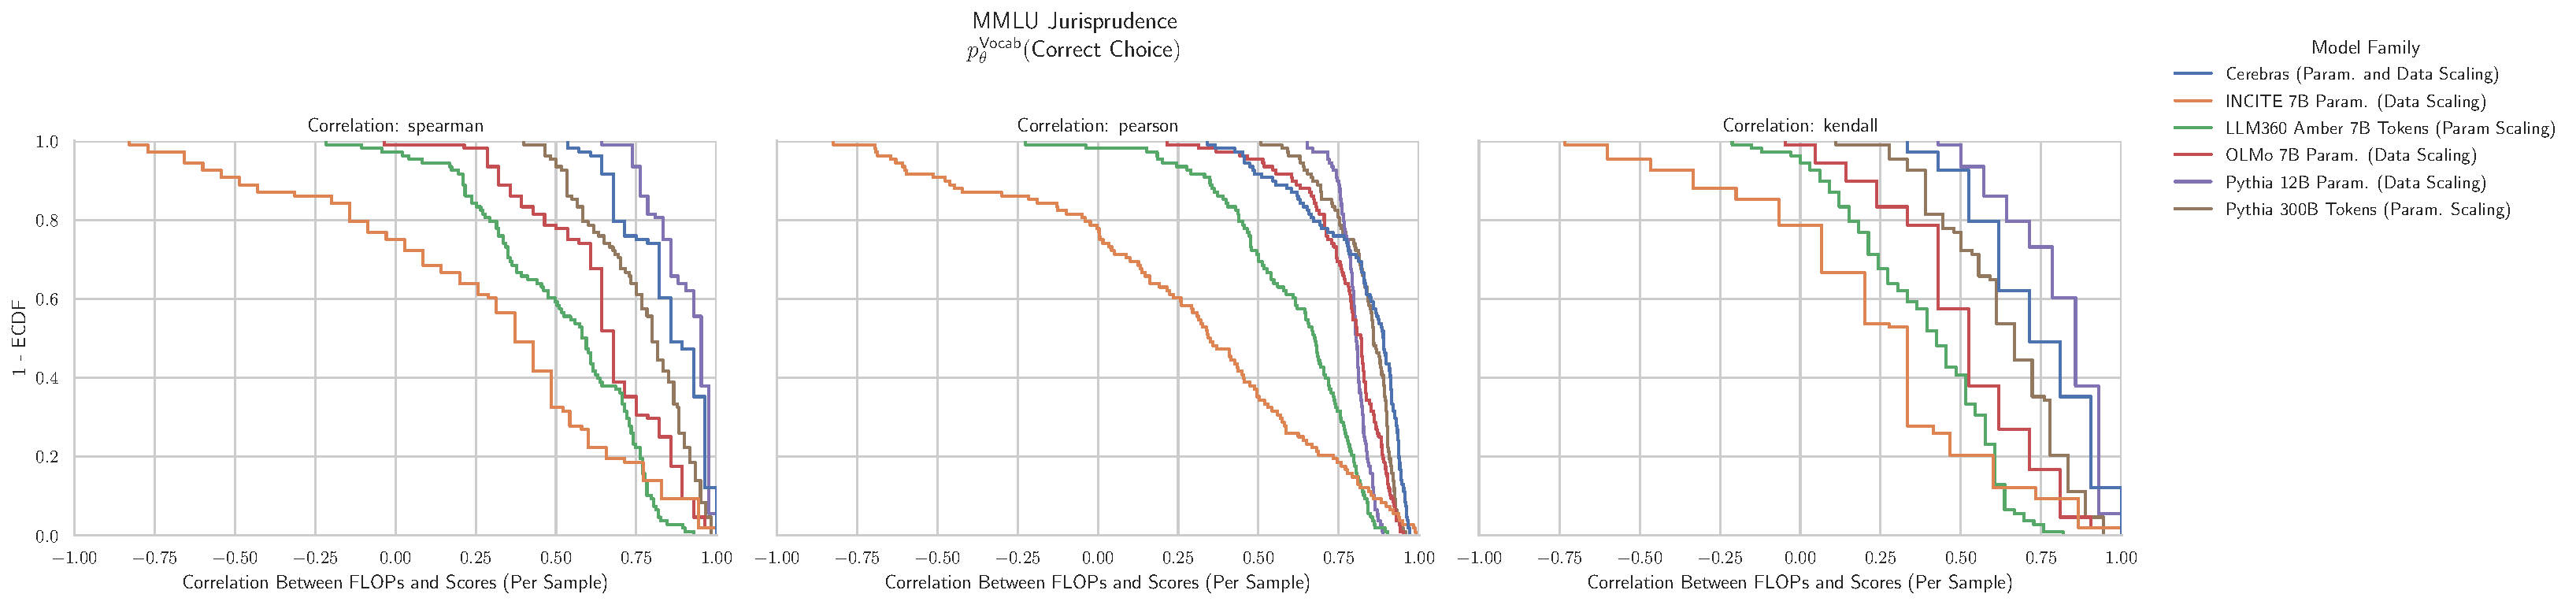
\includegraphics[width=\textwidth]{figures/correlations_between_scores_and_compute/correlation_distributions/mmlu_jurisprudence/mmlu_jurisprudence_prob_correct_vocab_ecdf_vs_correlation_score_by_modelfamily_split_correlation_metric.pdf}
    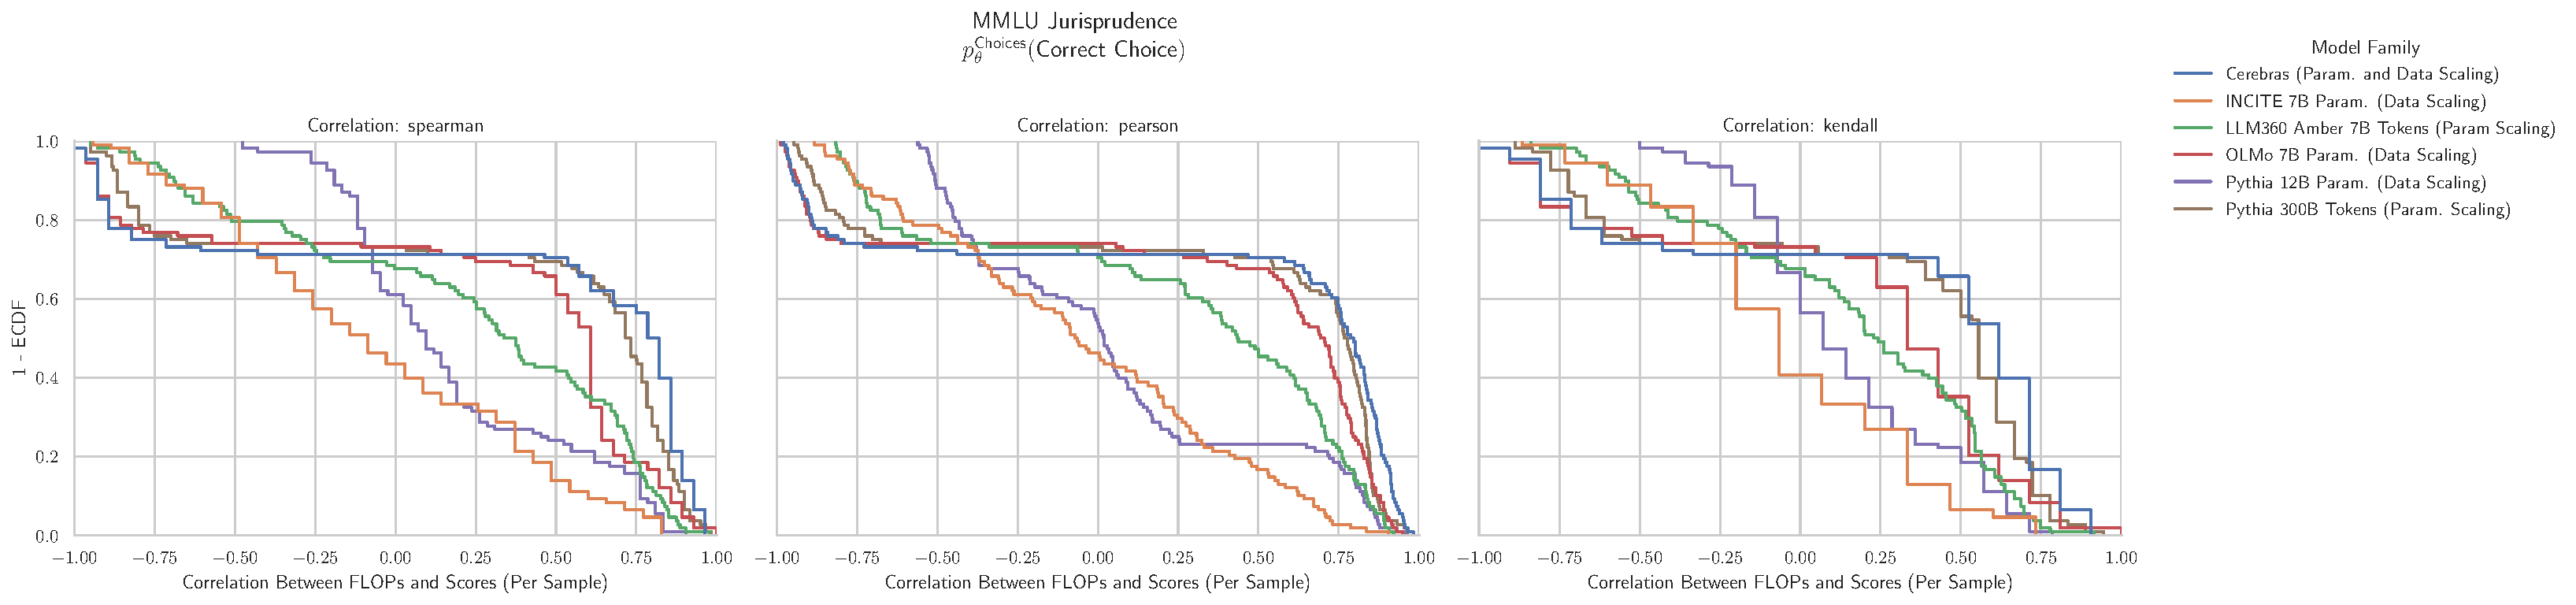
\includegraphics[width=\textwidth]{figures/correlations_between_scores_and_compute/correlation_distributions/mmlu_jurisprudence/mmlu_jurisprudence_prob_correct_choices_ecdf_vs_correlation_score_by_modelfamily_split_correlation_metric.pdf}
    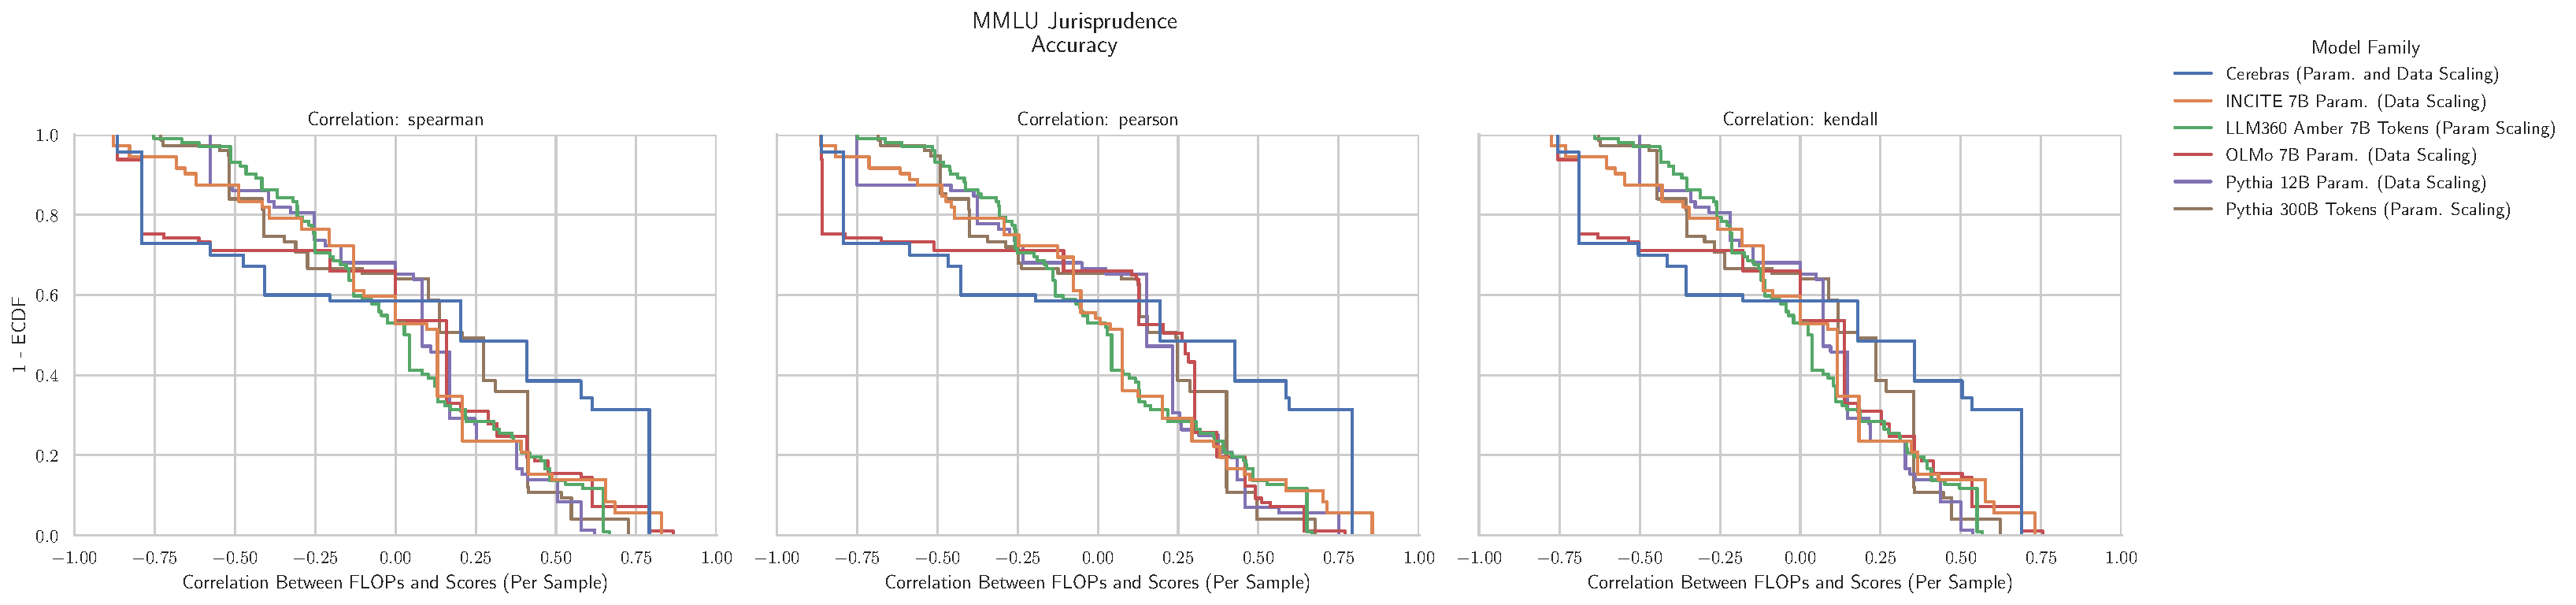
\includegraphics[width=\textwidth]{figures/correlations_between_scores_and_compute/correlation_distributions/mmlu_jurisprudence/mmlu_jurisprudence_acc_ecdf_vs_correlation_score_by_modelfamily_split_correlation_metric.pdf}
    \caption{\textbf{MMLU Jurisprudence: Downstream performance is computed via a sequence of transformations that deteriorate correlations between scores and pretraining compute.}}
    \label{app:fig:compute_score_distribution_mmlu_jurisprudence}
\end{figure}


\clearpage
\subsection{NLP Benchmark: MMLU Logical Fallacies \cite{hendrycks2020mmlu}}

\begin{figure}[h!]
    \centering
    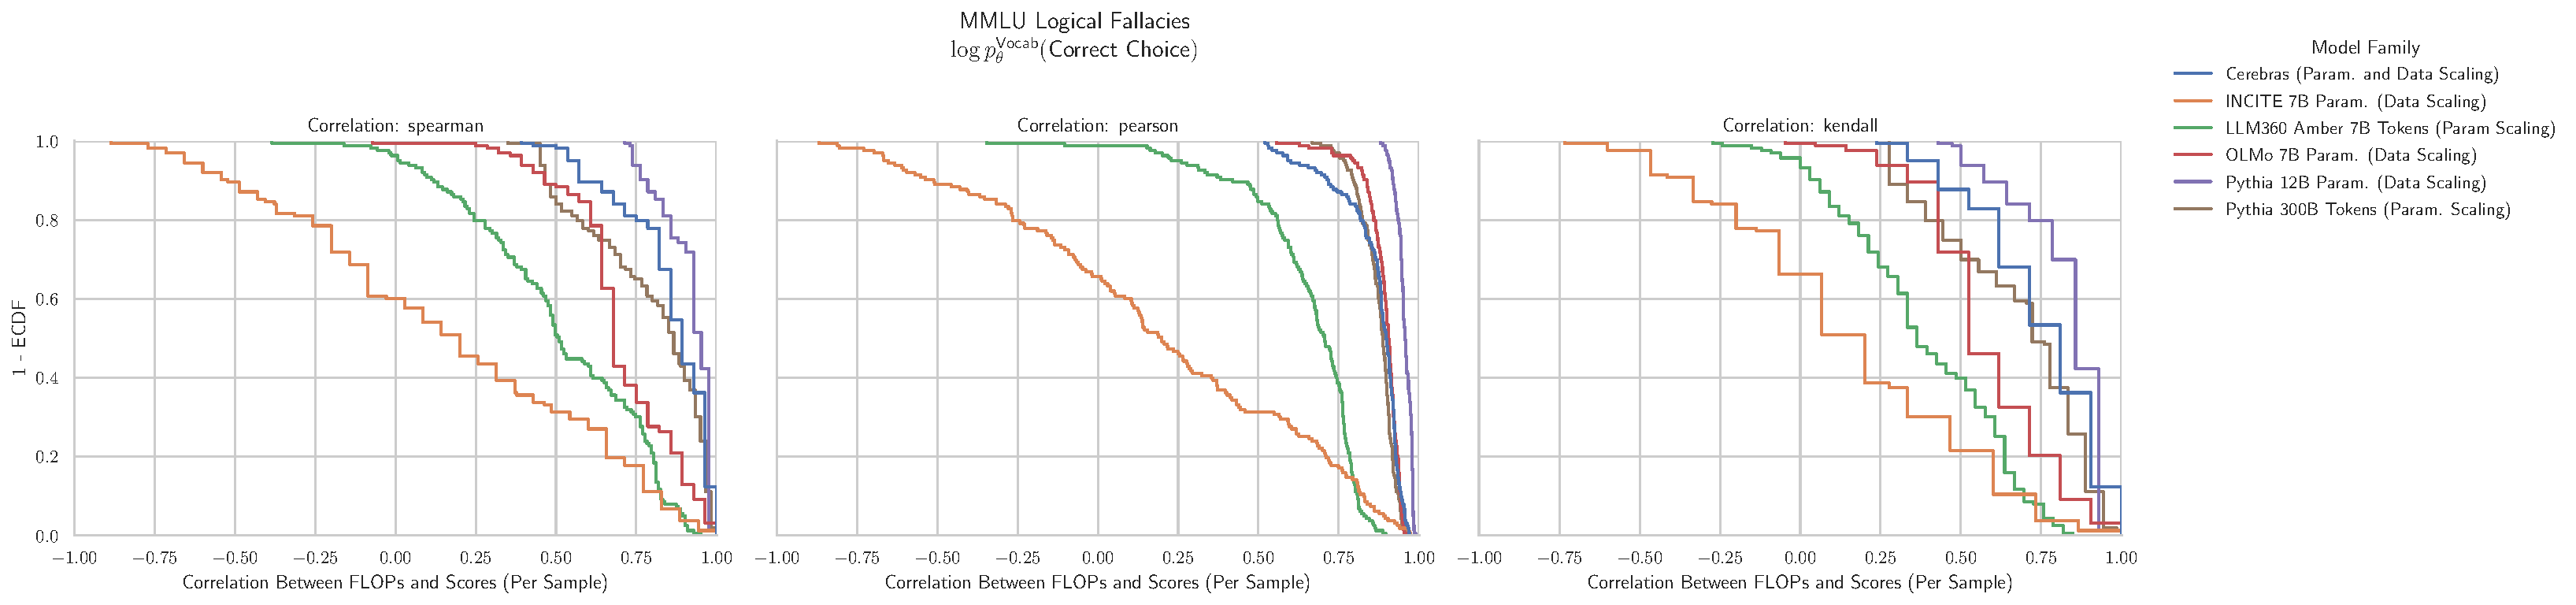
\includegraphics[width=\textwidth]{figures/correlations_between_scores_and_compute/correlation_distributions/mmlu_logical_fallacies/mmlu_logical_fallacies_log_likelihood_correct_ecdf_vs_correlation_score_by_modelfamily_split_correlation_metric.pdf}
    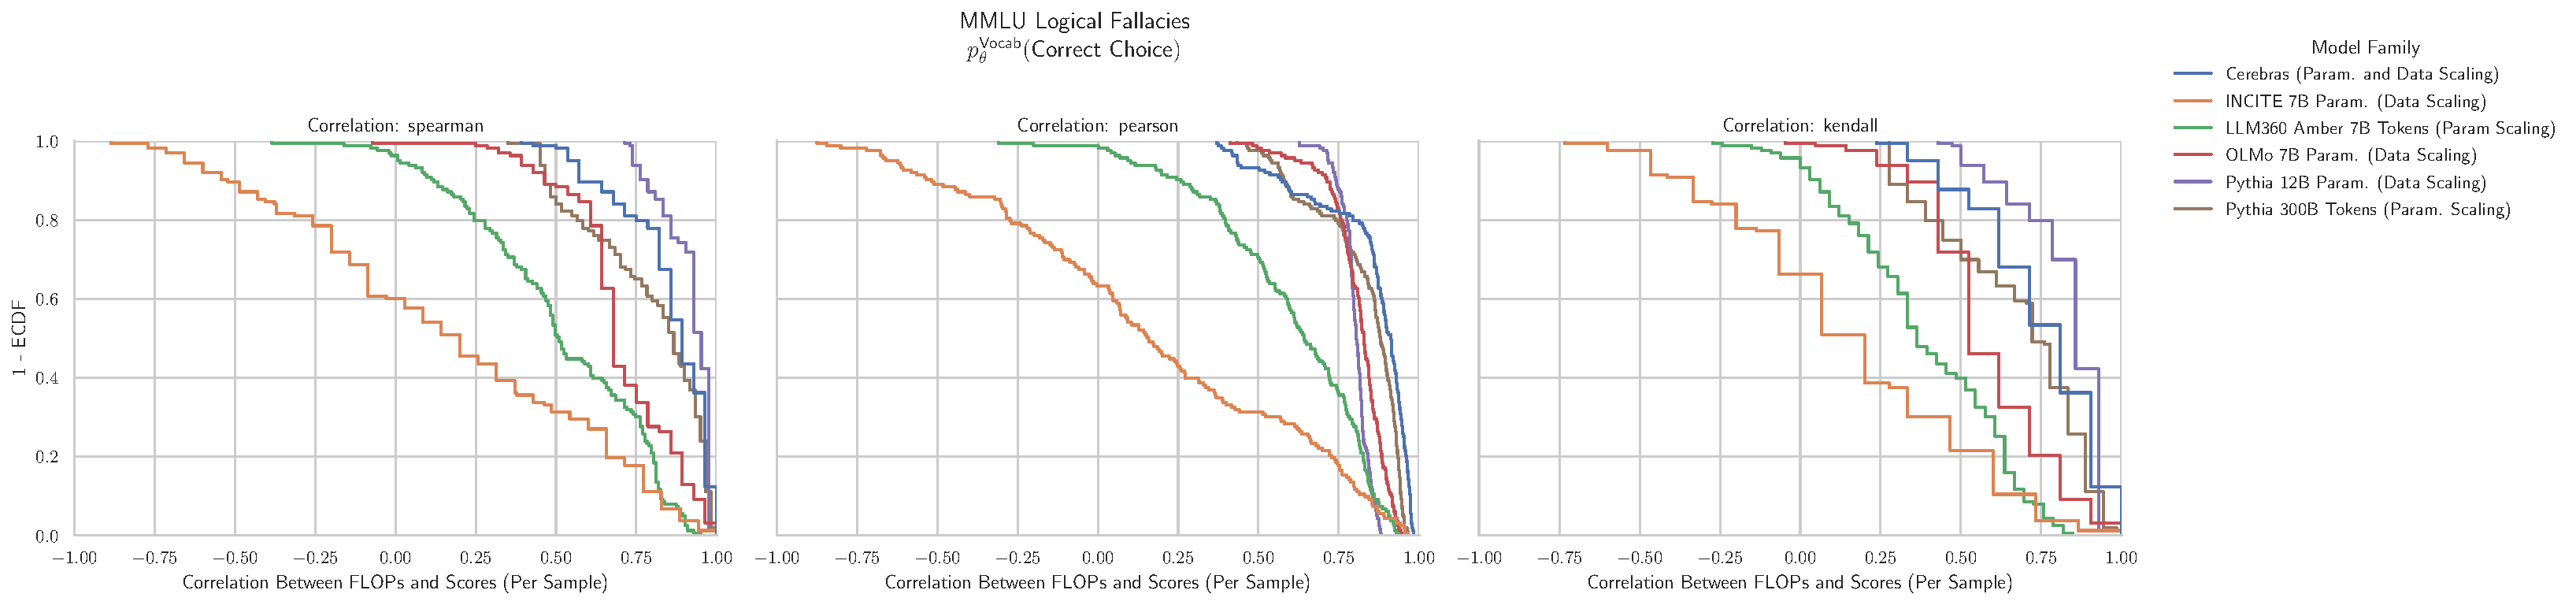
\includegraphics[width=\textwidth]{figures/correlations_between_scores_and_compute/correlation_distributions/mmlu_logical_fallacies/mmlu_logical_fallacies_prob_correct_vocab_ecdf_vs_correlation_score_by_modelfamily_split_correlation_metric.pdf}
    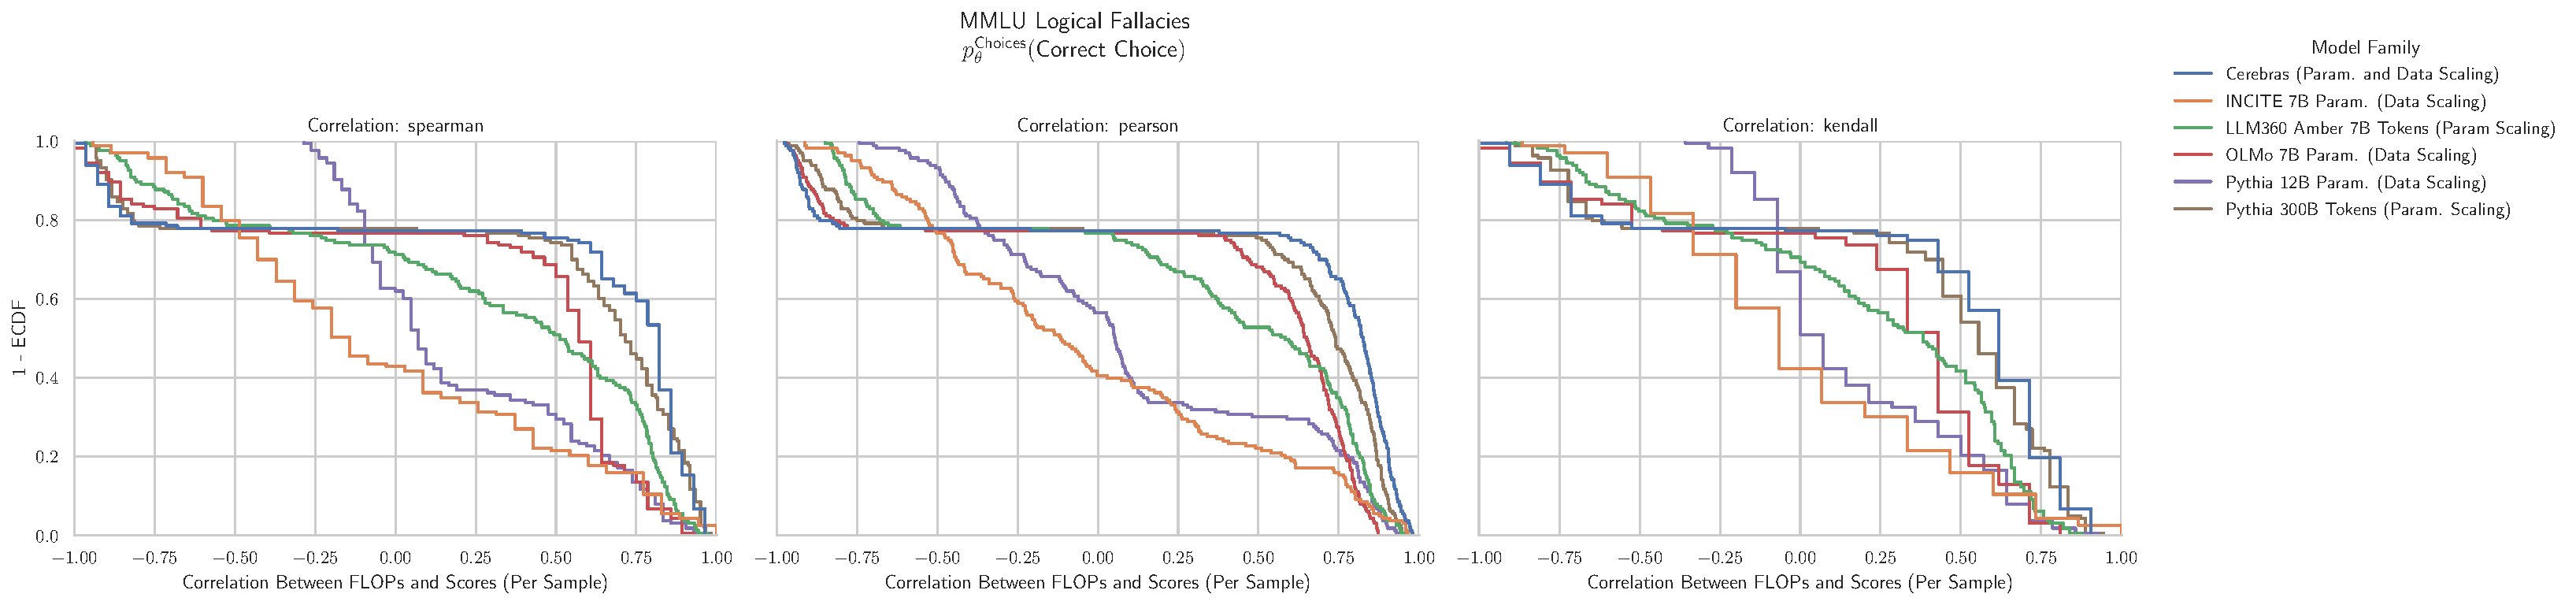
\includegraphics[width=\textwidth]{figures/correlations_between_scores_and_compute/correlation_distributions/mmlu_logical_fallacies/mmlu_logical_fallacies_prob_correct_choices_ecdf_vs_correlation_score_by_modelfamily_split_correlation_metric.pdf}
    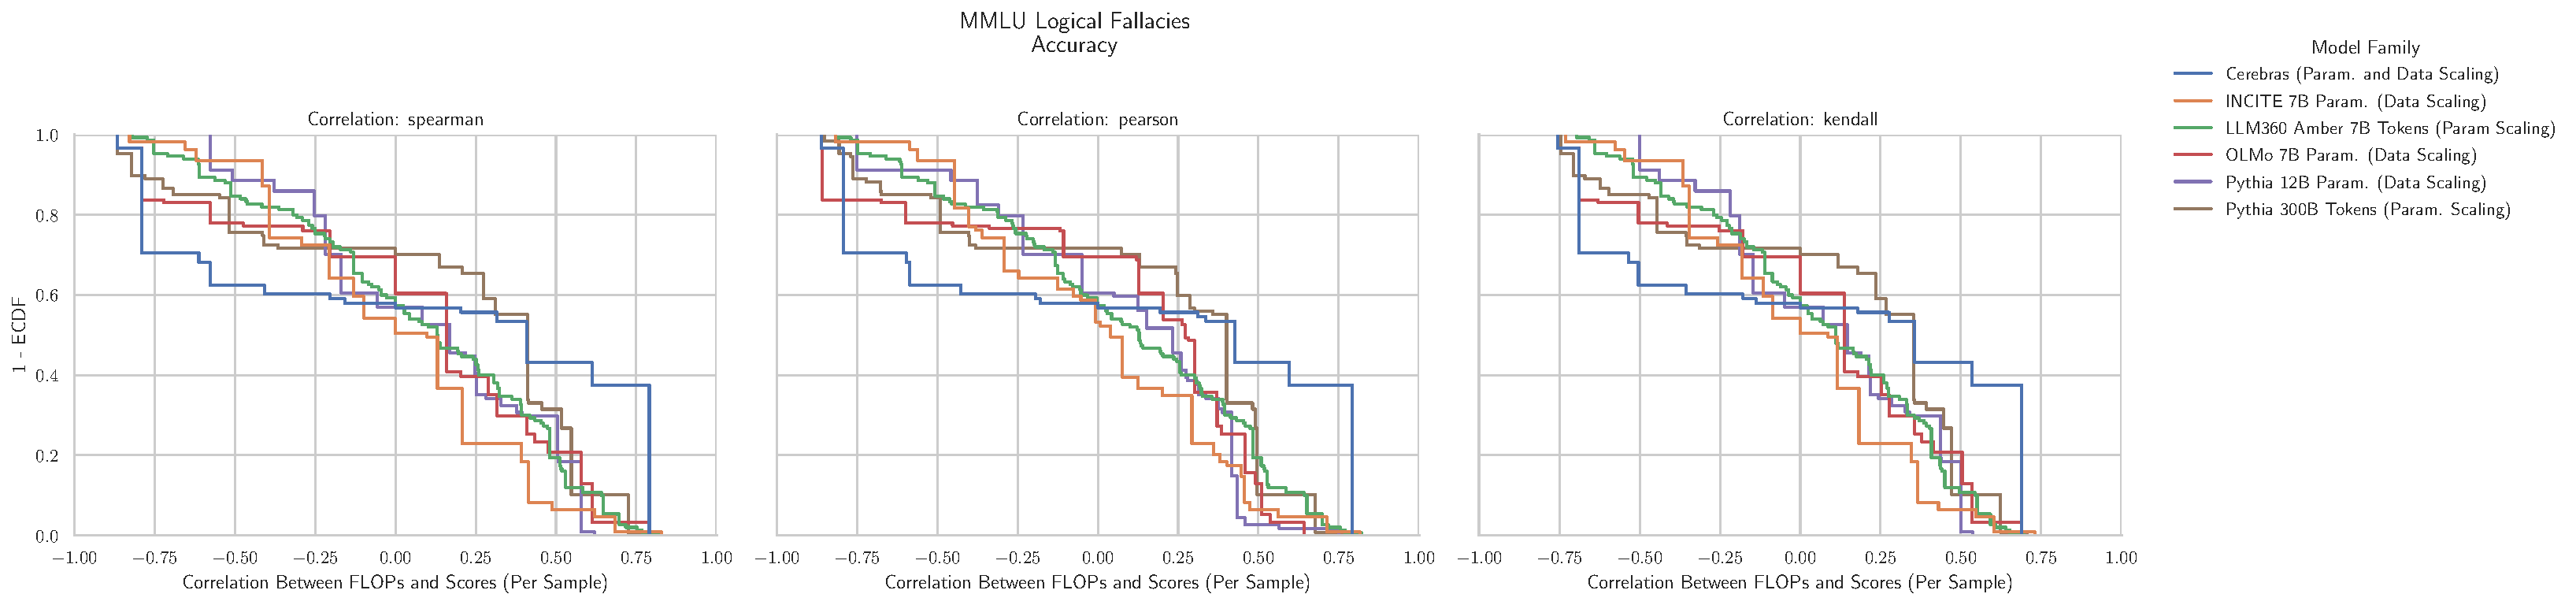
\includegraphics[width=\textwidth]{figures/correlations_between_scores_and_compute/correlation_distributions/mmlu_logical_fallacies/mmlu_logical_fallacies_acc_ecdf_vs_correlation_score_by_modelfamily_split_correlation_metric.pdf}
    \caption{\textbf{MMLU Logical Fallacies: Downstream performance is computed via a sequence of transformations that deteriorate correlations between scores and pretraining compute.}}
    \label{app:fig:compute_score_distribution_mmlu_logical_fallacies}
\end{figure}


\clearpage
\subsection{NLP Benchmark: MMLU Machine Learning \cite{hendrycks2020mmlu}}

\begin{figure}[h!]
    \centering
    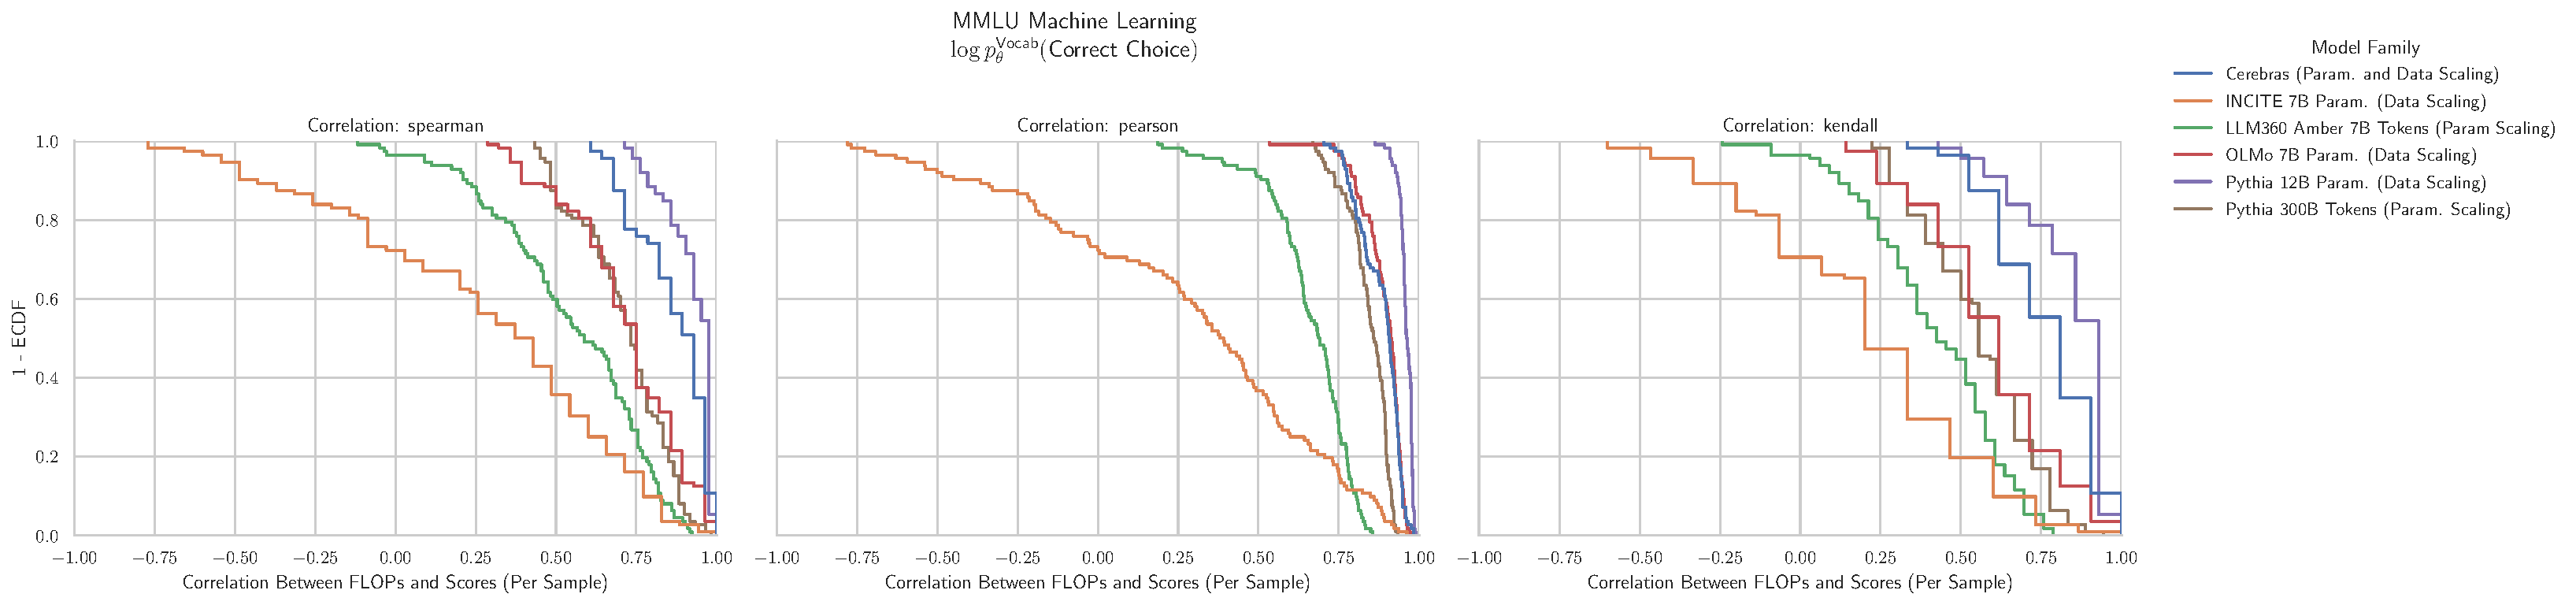
\includegraphics[width=\textwidth]{figures/correlations_between_scores_and_compute/correlation_distributions/mmlu_machine_learning/mmlu_machine_learning_log_likelihood_correct_ecdf_vs_correlation_score_by_modelfamily_split_correlation_metric.pdf}
    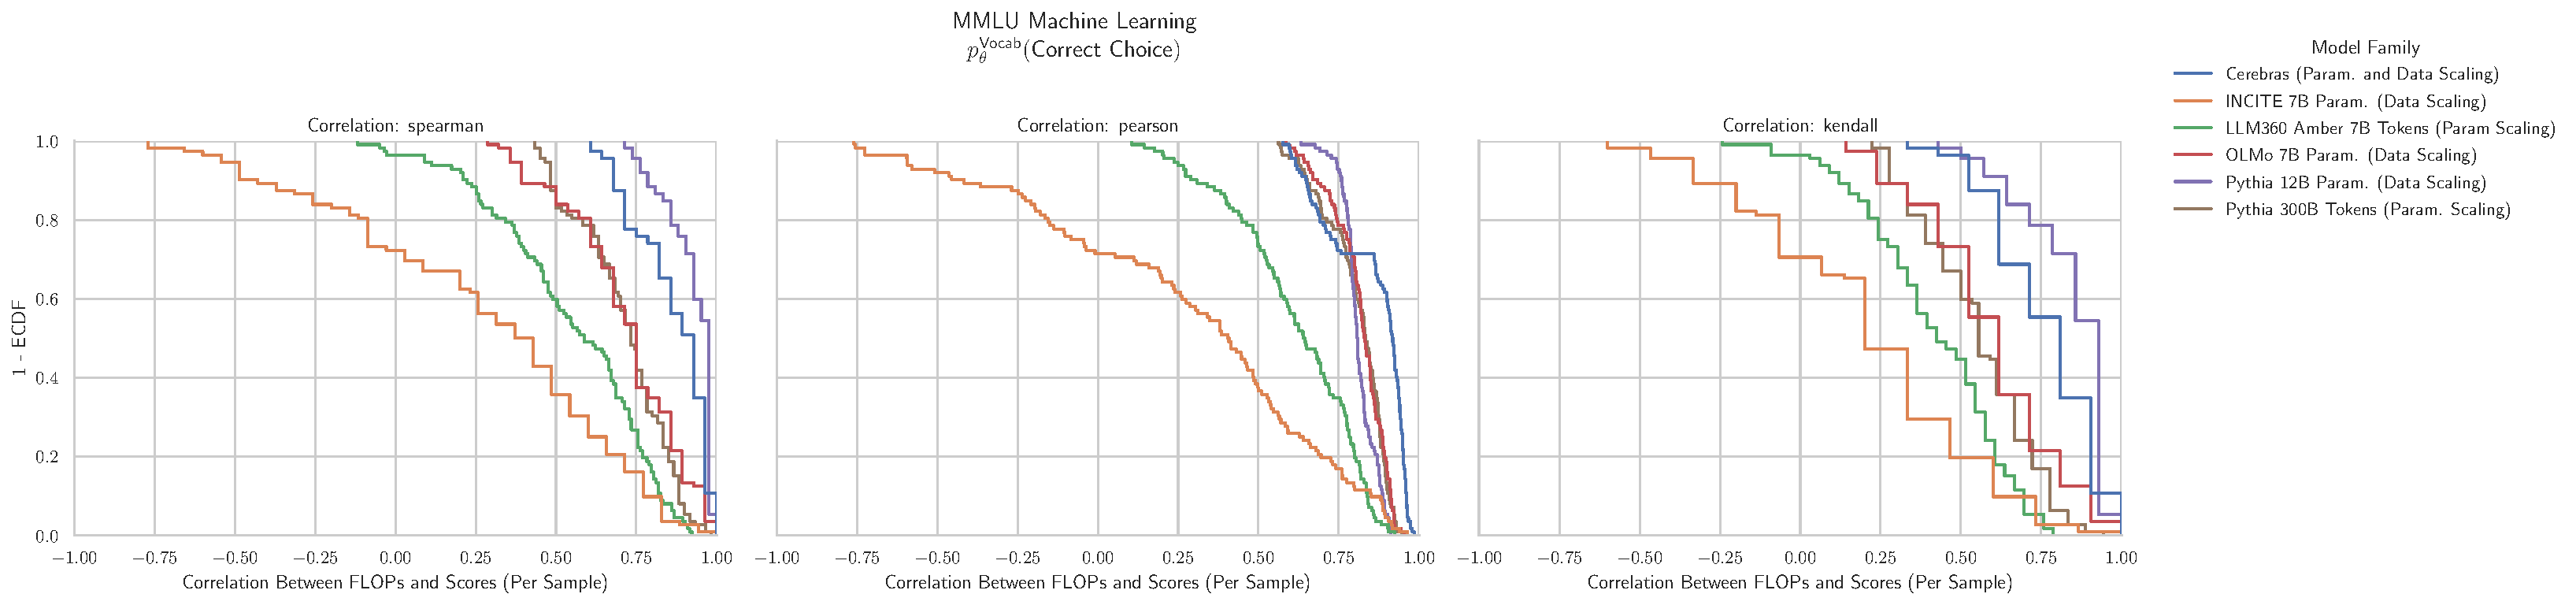
\includegraphics[width=\textwidth]{figures/correlations_between_scores_and_compute/correlation_distributions/mmlu_machine_learning/mmlu_machine_learning_prob_correct_vocab_ecdf_vs_correlation_score_by_modelfamily_split_correlation_metric.pdf}
    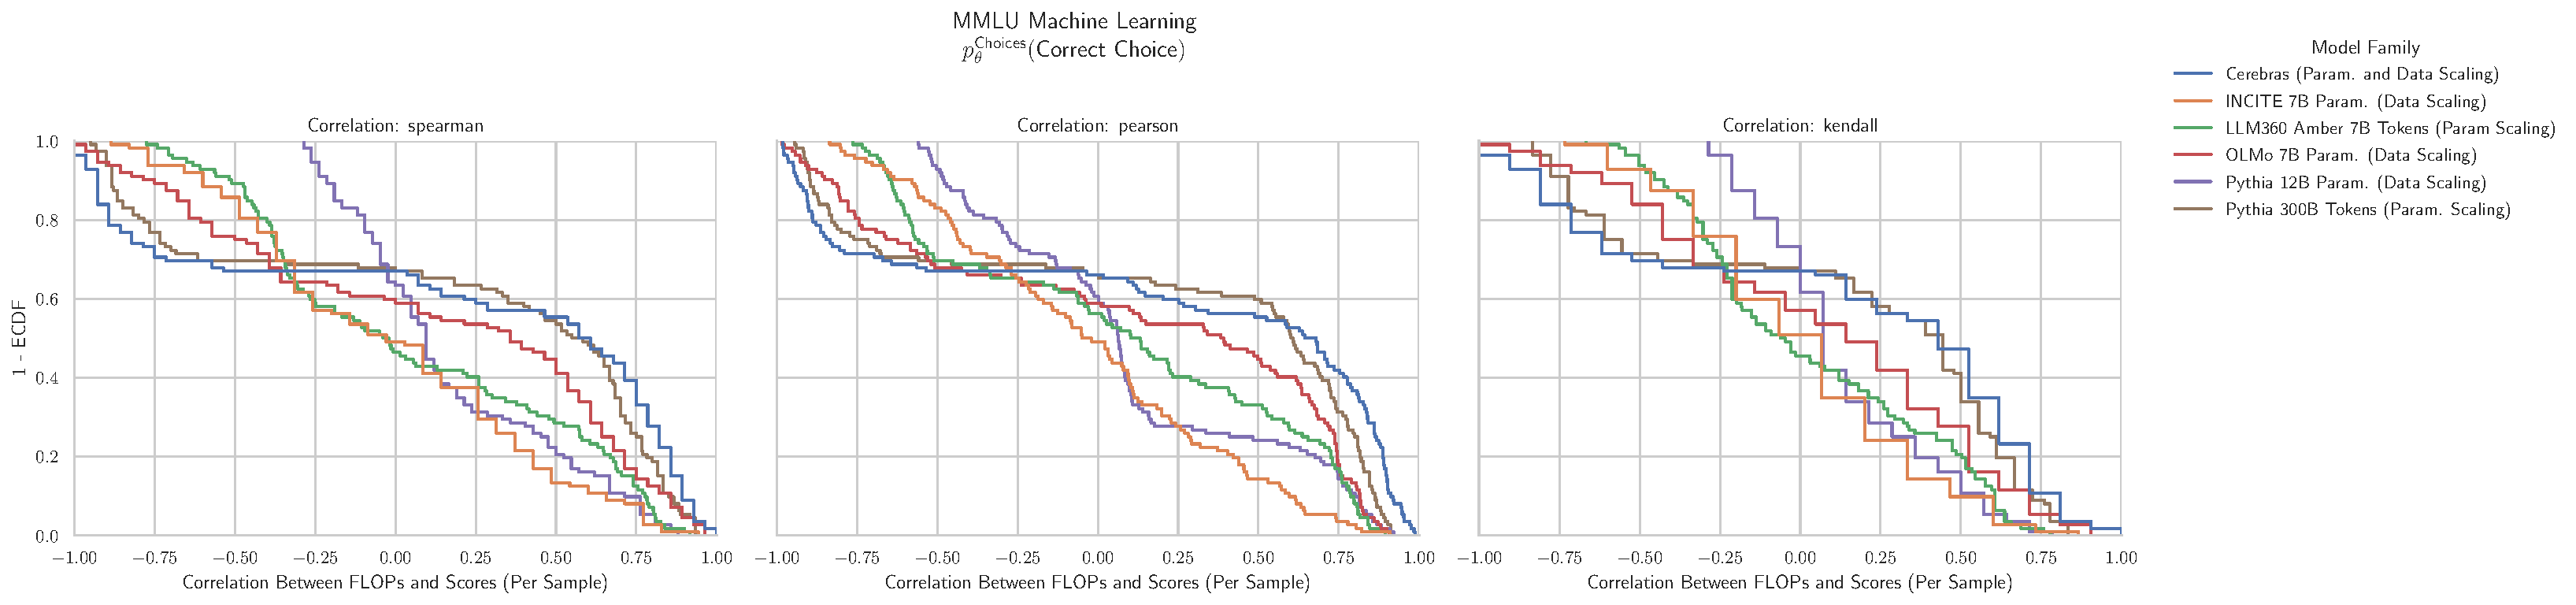
\includegraphics[width=\textwidth]{figures/correlations_between_scores_and_compute/correlation_distributions/mmlu_machine_learning/mmlu_machine_learning_prob_correct_choices_ecdf_vs_correlation_score_by_modelfamily_split_correlation_metric.pdf}
    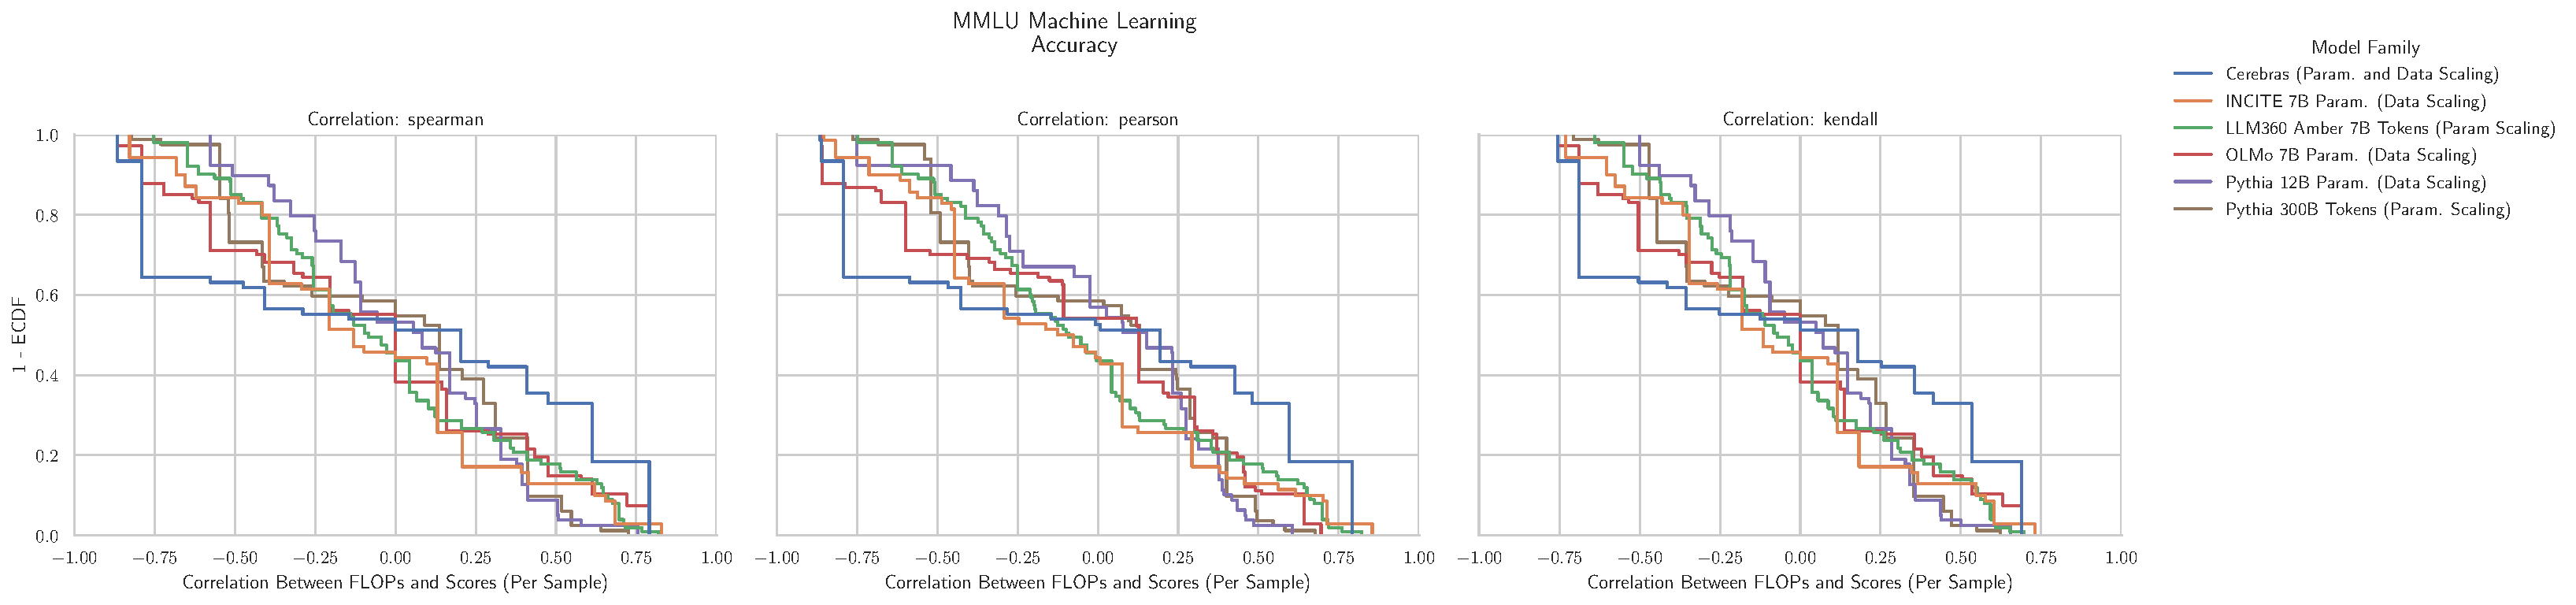
\includegraphics[width=\textwidth]{figures/correlations_between_scores_and_compute/correlation_distributions/mmlu_machine_learning/mmlu_machine_learning_acc_ecdf_vs_correlation_score_by_modelfamily_split_correlation_metric.pdf}
    \caption{\textbf{MMLU Machine Learning: Downstream performance is computed via a sequence of transformations that deteriorate correlations between scores and pretraining compute.}}
    \label{app:fig:compute_score_distribution_mmlu_machine_learning}
\end{figure}

\clearpage
\subsection{NLP Benchmark: MMLU Management \cite{hendrycks2020mmlu}}

\begin{figure}[h!]
    \centering
    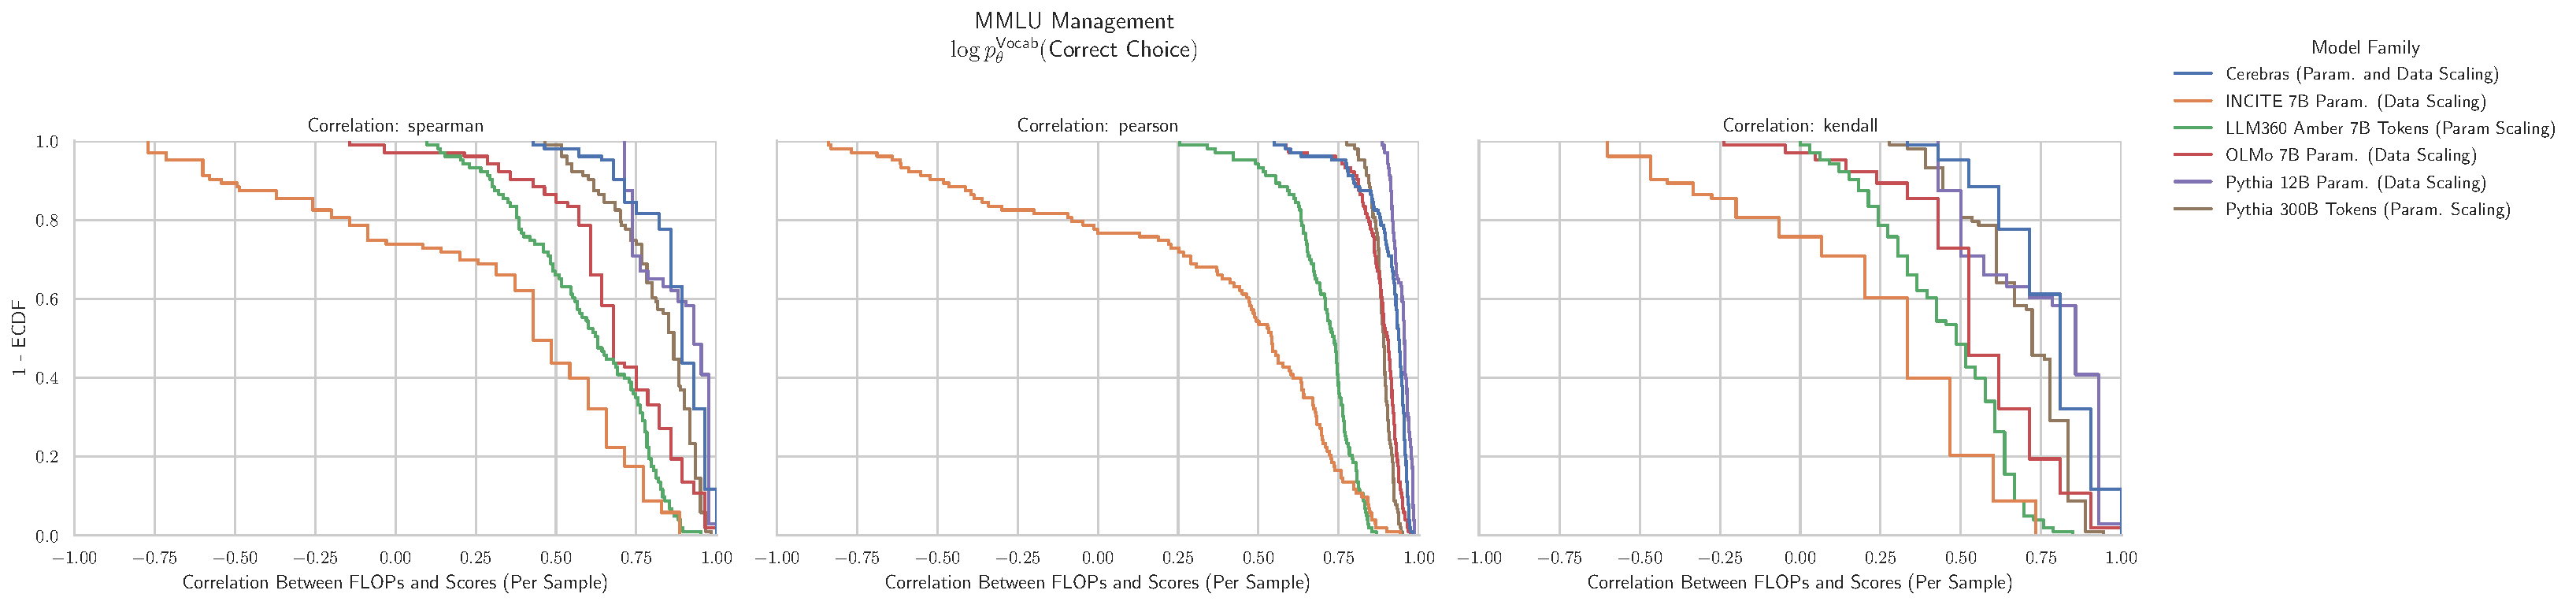
\includegraphics[width=\textwidth]{figures/correlations_between_scores_and_compute/correlation_distributions/mmlu_management/mmlu_management_log_likelihood_correct_ecdf_vs_correlation_score_by_modelfamily_split_correlation_metric.pdf}
    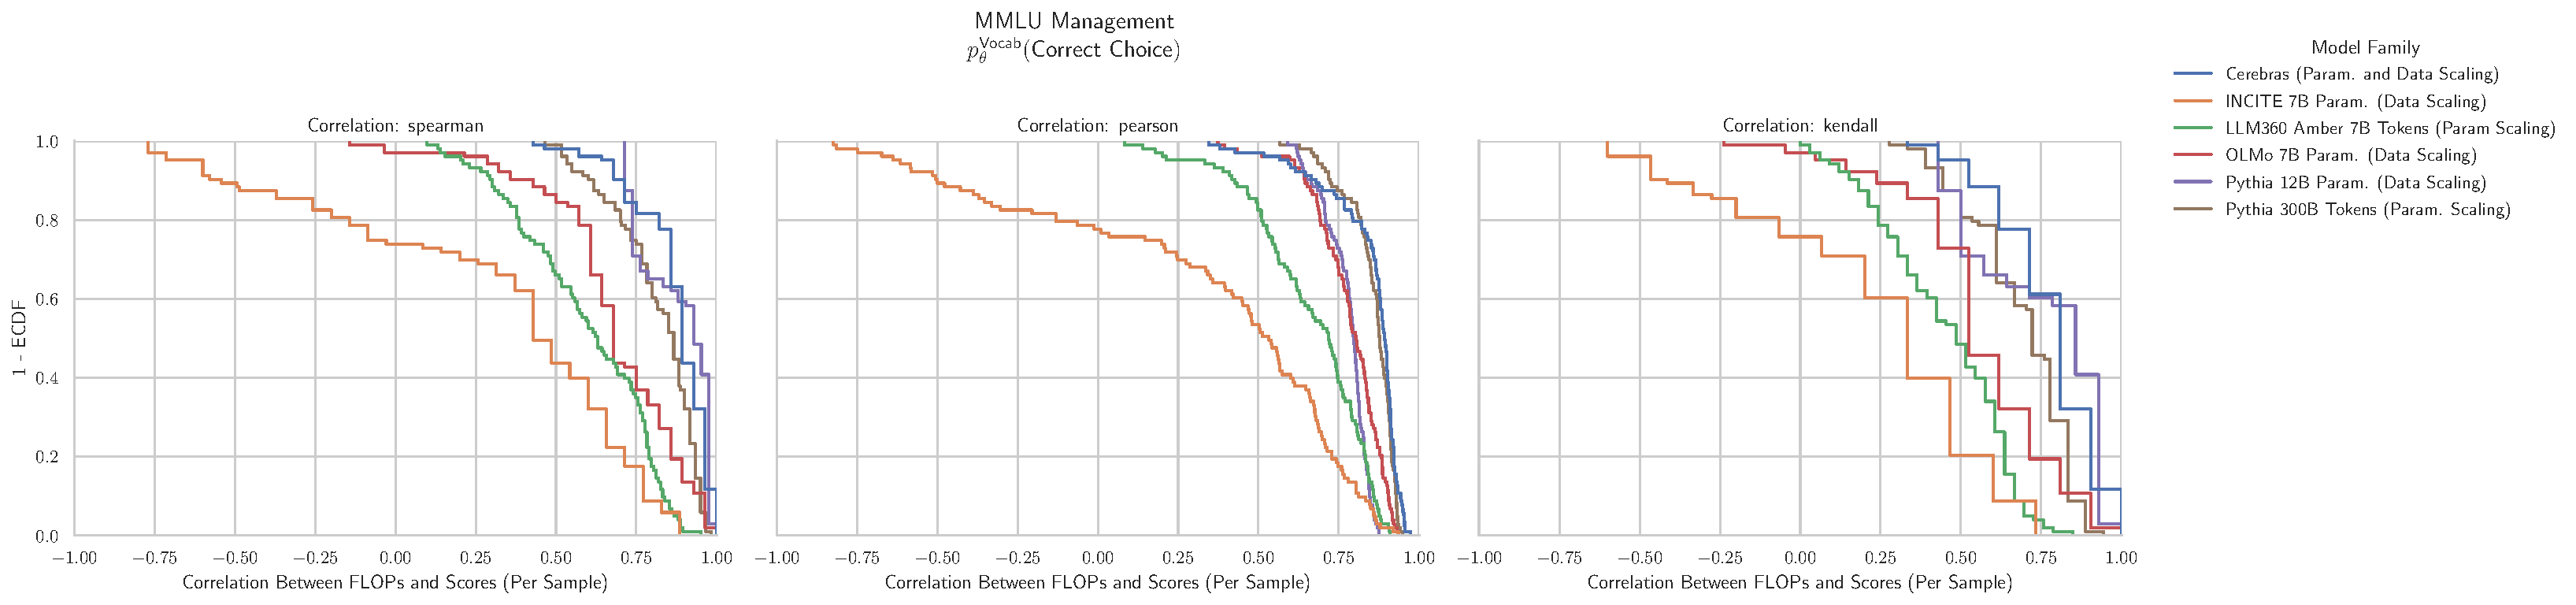
\includegraphics[width=\textwidth]{figures/correlations_between_scores_and_compute/correlation_distributions/mmlu_management/mmlu_management_prob_correct_vocab_ecdf_vs_correlation_score_by_modelfamily_split_correlation_metric.pdf}
    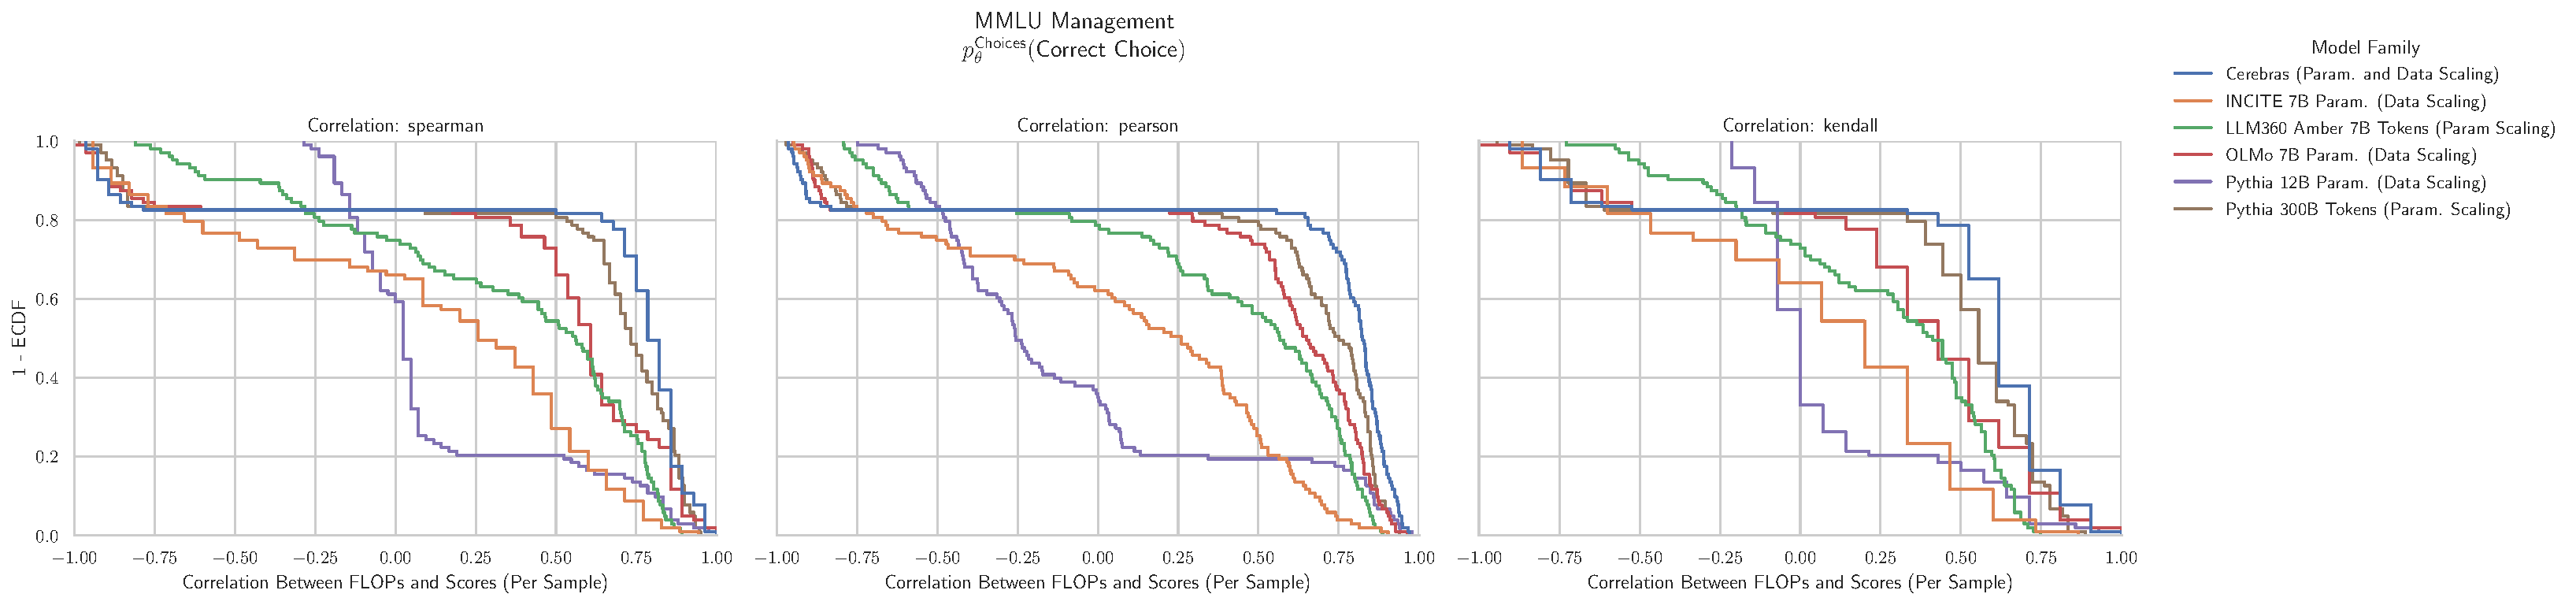
\includegraphics[width=\textwidth]{figures/correlations_between_scores_and_compute/correlation_distributions/mmlu_management/mmlu_management_prob_correct_choices_ecdf_vs_correlation_score_by_modelfamily_split_correlation_metric.pdf}
    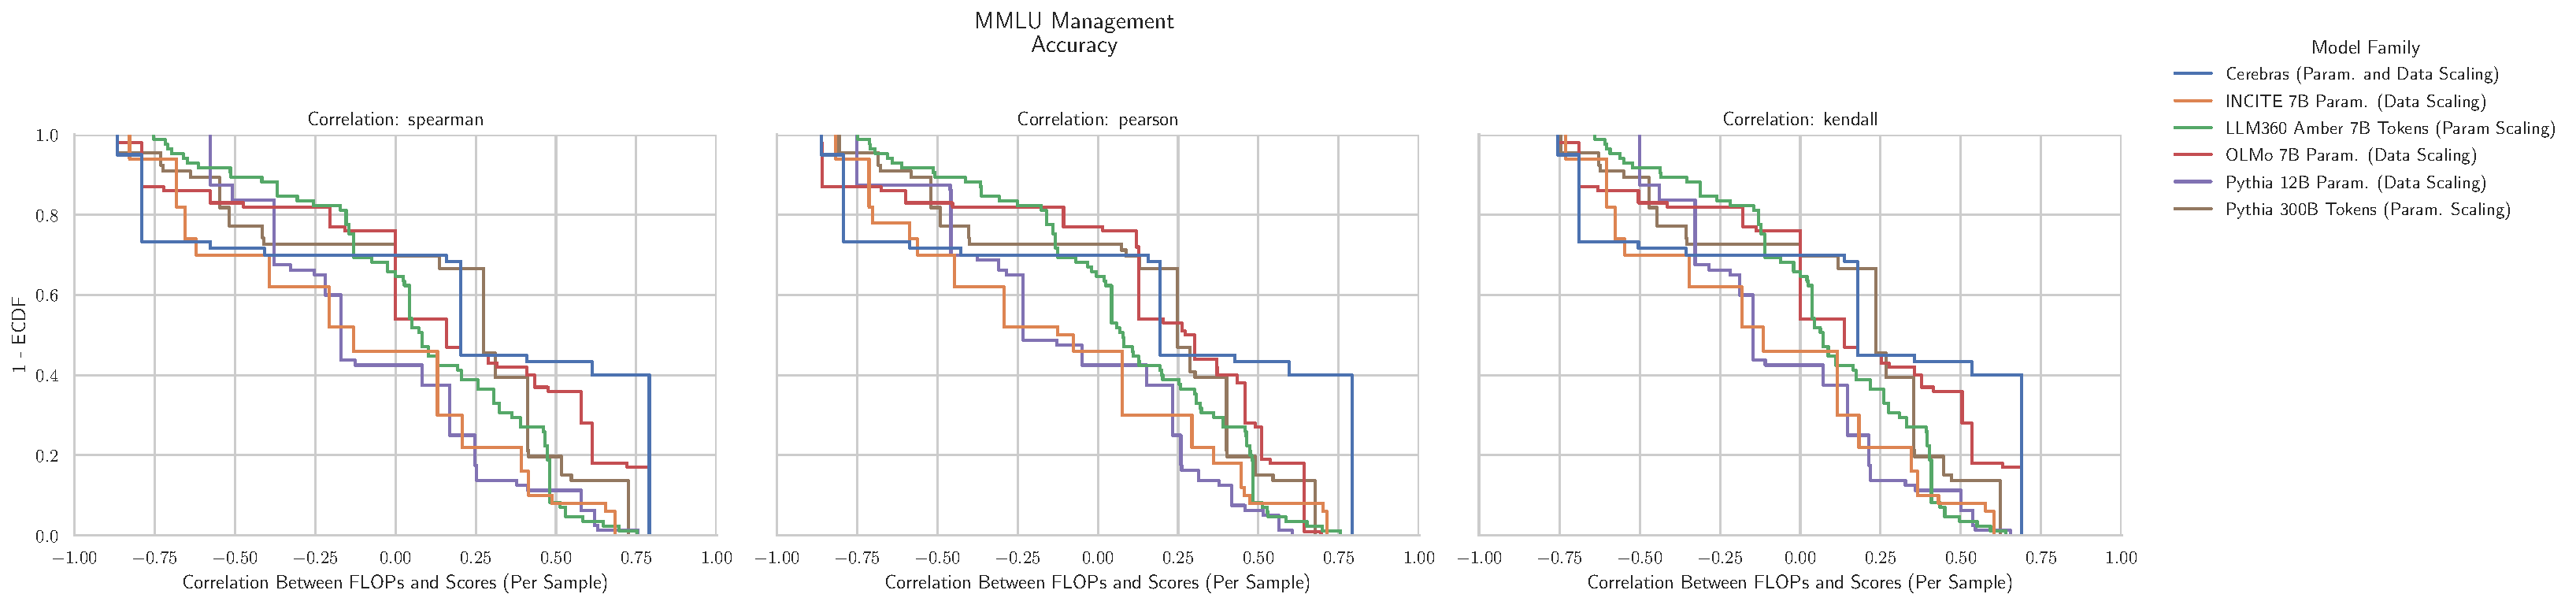
\includegraphics[width=\textwidth]{figures/correlations_between_scores_and_compute/correlation_distributions/mmlu_management/mmlu_management_acc_ecdf_vs_correlation_score_by_modelfamily_split_correlation_metric.pdf}
    \caption{\textbf{MMLU Management: Downstream performance is computed via a sequence of transformations that deteriorate correlations between scores and pretraining compute.}}
    \label{app:fig:compute_score_distribution_mmlu_management}
\end{figure}

\clearpage
\subsection{NLP Benchmark: MMLU Marketing \cite{hendrycks2020mmlu}}

\begin{figure}[h!]
    \centering
    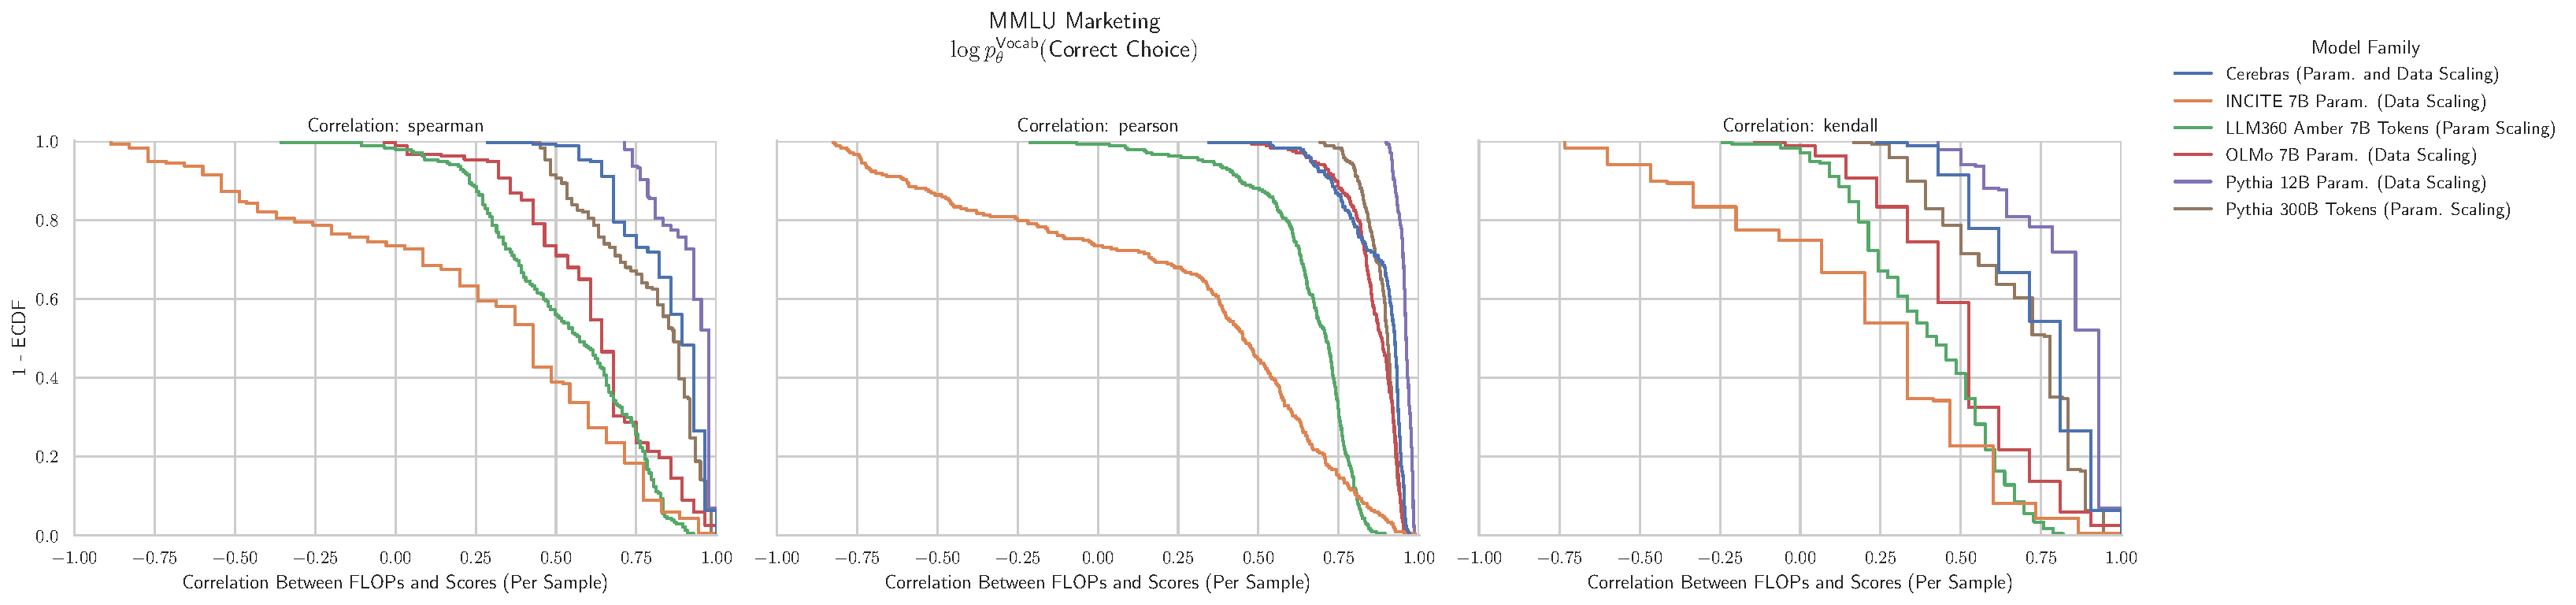
\includegraphics[width=\textwidth]{figures/correlations_between_scores_and_compute/correlation_distributions/mmlu_marketing/mmlu_marketing_log_likelihood_correct_ecdf_vs_correlation_score_by_modelfamily_split_correlation_metric.pdf}
    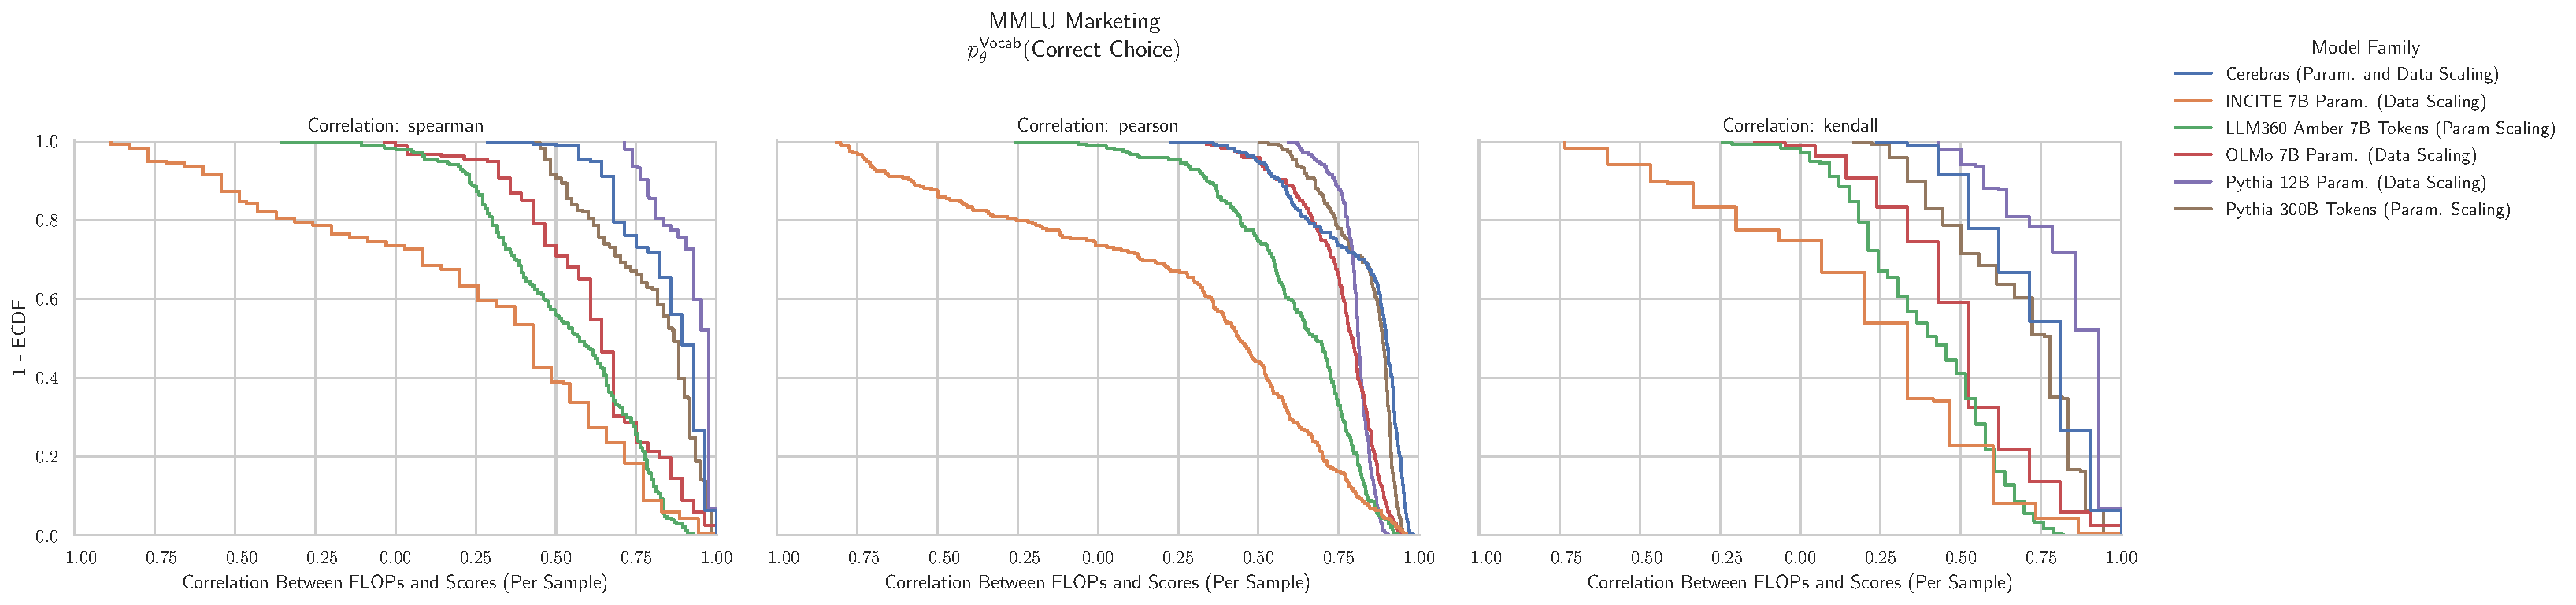
\includegraphics[width=\textwidth]{figures/correlations_between_scores_and_compute/correlation_distributions/mmlu_marketing/mmlu_marketing_prob_correct_vocab_ecdf_vs_correlation_score_by_modelfamily_split_correlation_metric.pdf}
    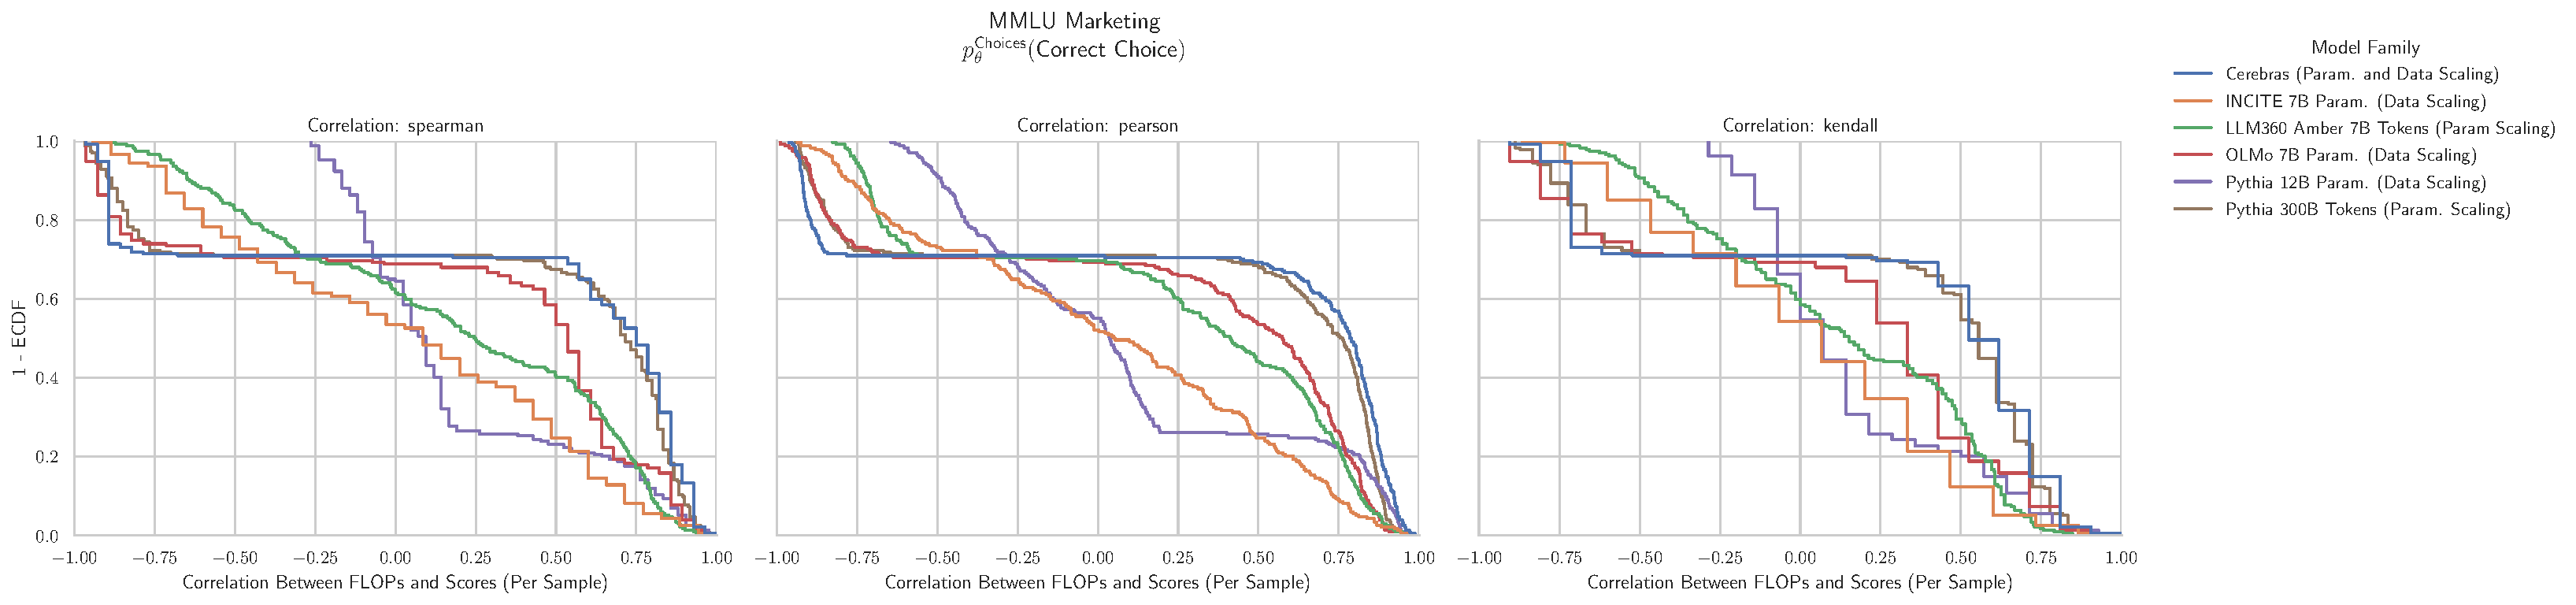
\includegraphics[width=\textwidth]{figures/correlations_between_scores_and_compute/correlation_distributions/mmlu_marketing/mmlu_marketing_prob_correct_choices_ecdf_vs_correlation_score_by_modelfamily_split_correlation_metric.pdf}
    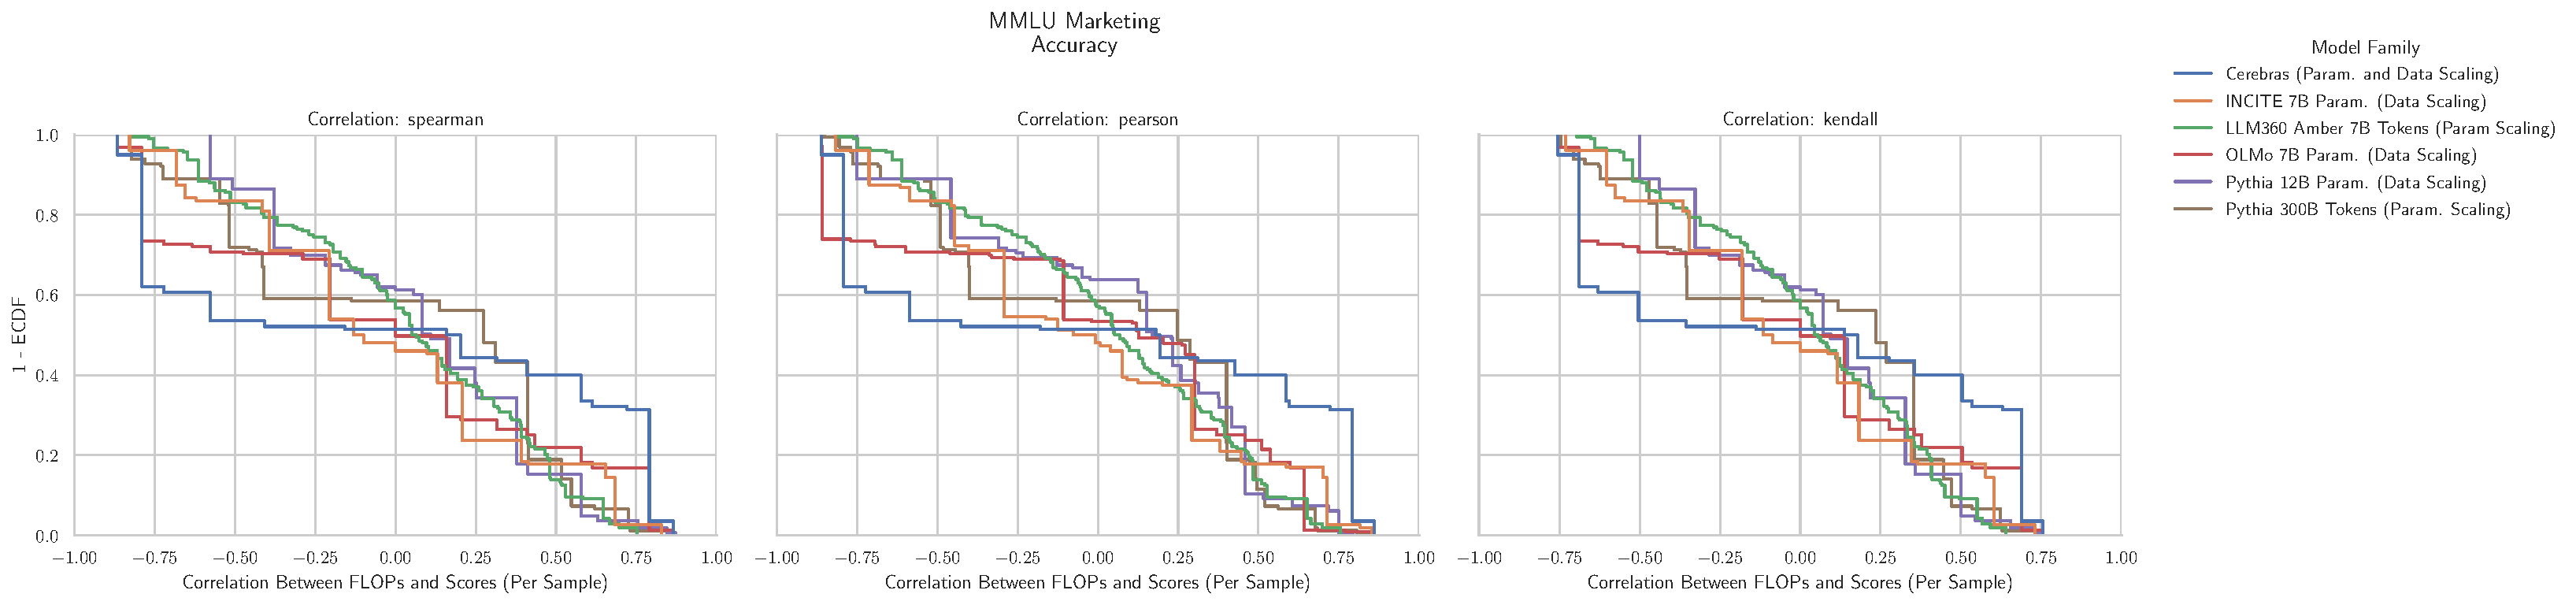
\includegraphics[width=\textwidth]{figures/correlations_between_scores_and_compute/correlation_distributions/mmlu_marketing/mmlu_marketing_acc_ecdf_vs_correlation_score_by_modelfamily_split_correlation_metric.pdf}
    \caption{\textbf{MMLU Marketing: Downstream performance is computed via a sequence of transformations that deteriorate correlations between scores and pretraining compute.}}
    \label{app:fig:compute_score_distribution_mmlu_marketing}
\end{figure}

\clearpage
\subsection{NLP Benchmark: MMLU Medical Genetics \cite{hendrycks2020mmlu}}

\begin{figure}[h!]
    \centering
    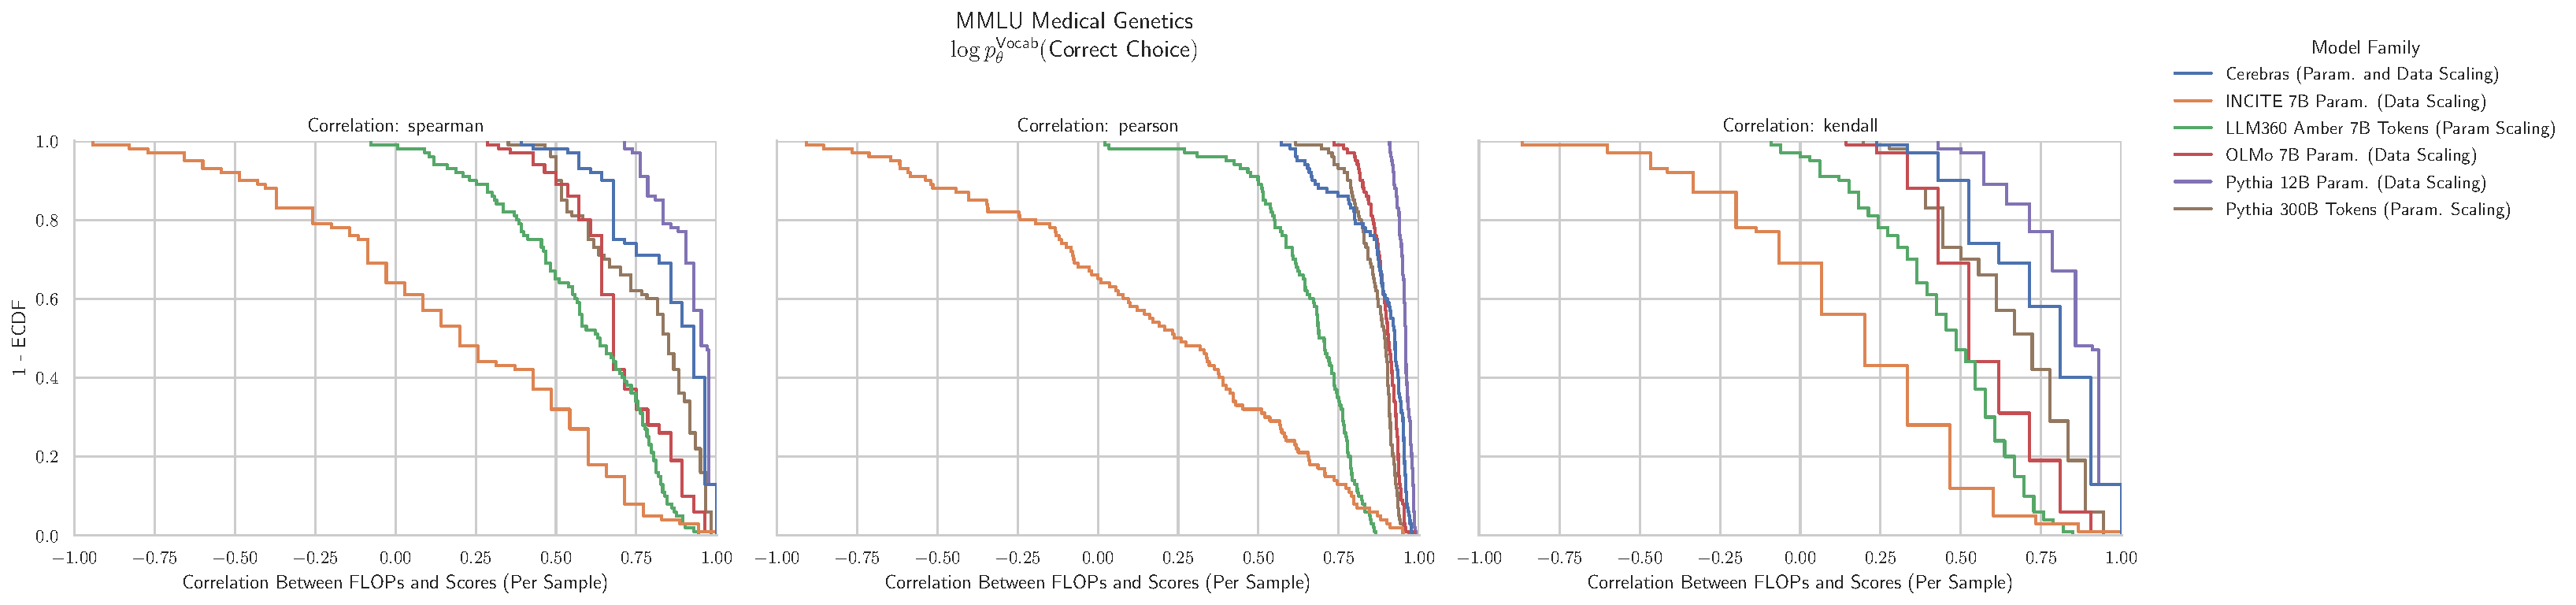
\includegraphics[width=\textwidth]{figures/correlations_between_scores_and_compute/correlation_distributions/mmlu_medical_genetics/mmlu_medical_genetics_log_likelihood_correct_ecdf_vs_correlation_score_by_modelfamily_split_correlation_metric.pdf}
    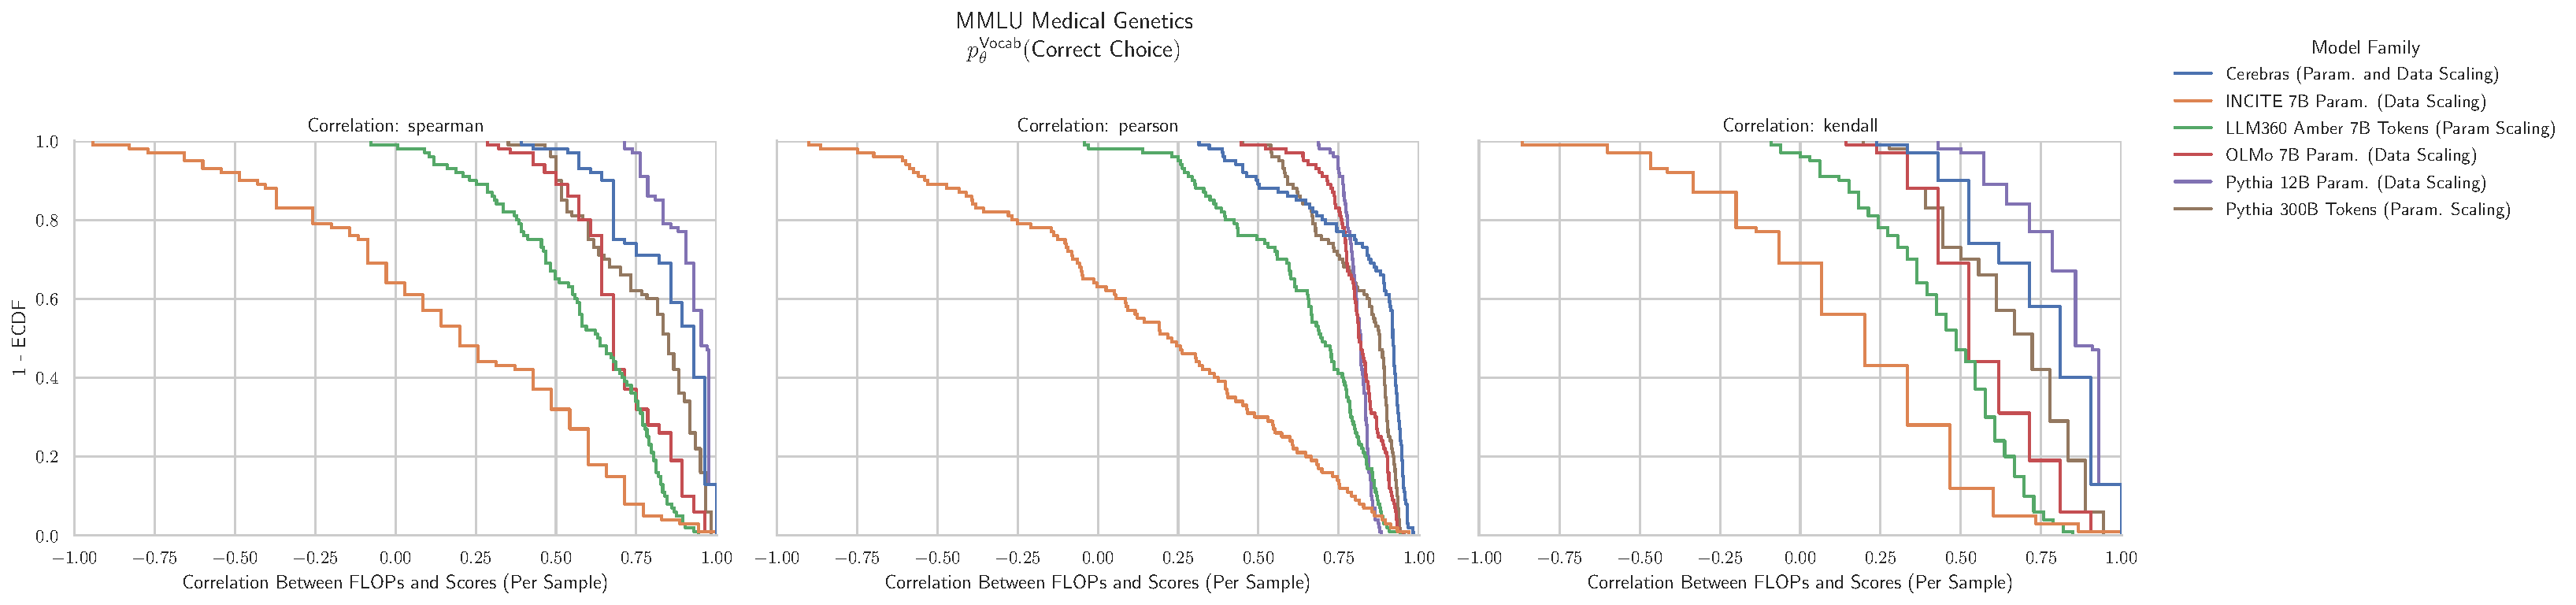
\includegraphics[width=\textwidth]{figures/correlations_between_scores_and_compute/correlation_distributions/mmlu_medical_genetics/mmlu_medical_genetics_prob_correct_vocab_ecdf_vs_correlation_score_by_modelfamily_split_correlation_metric.pdf}
    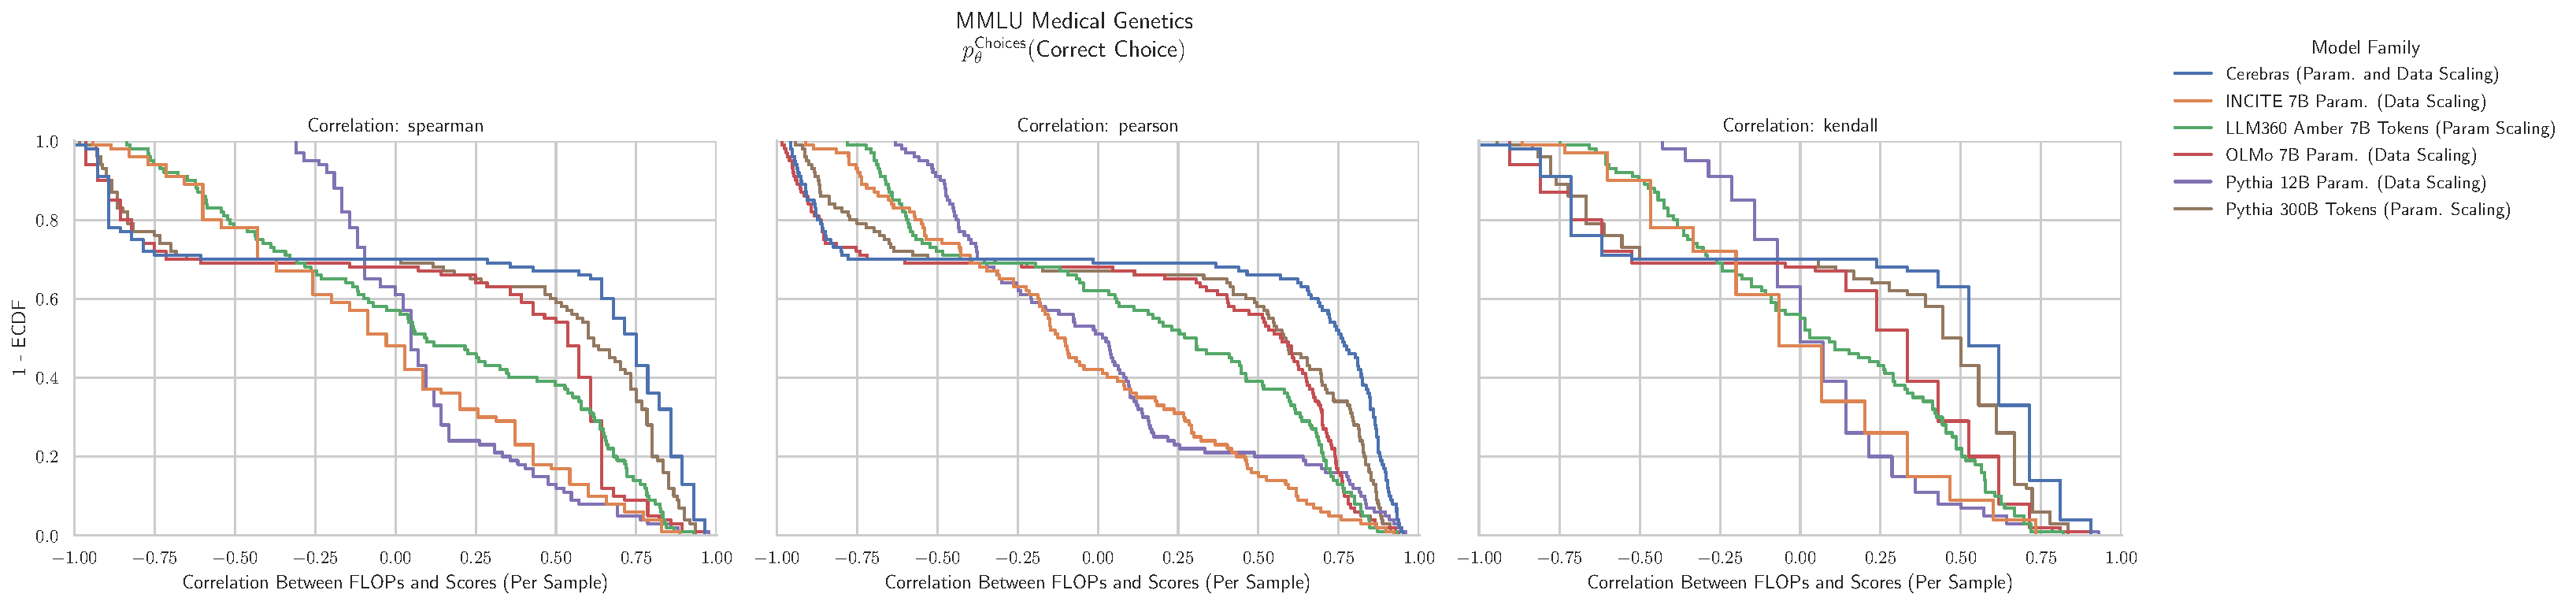
\includegraphics[width=\textwidth]{figures/correlations_between_scores_and_compute/correlation_distributions/mmlu_medical_genetics/mmlu_medical_genetics_prob_correct_choices_ecdf_vs_correlation_score_by_modelfamily_split_correlation_metric.pdf}
    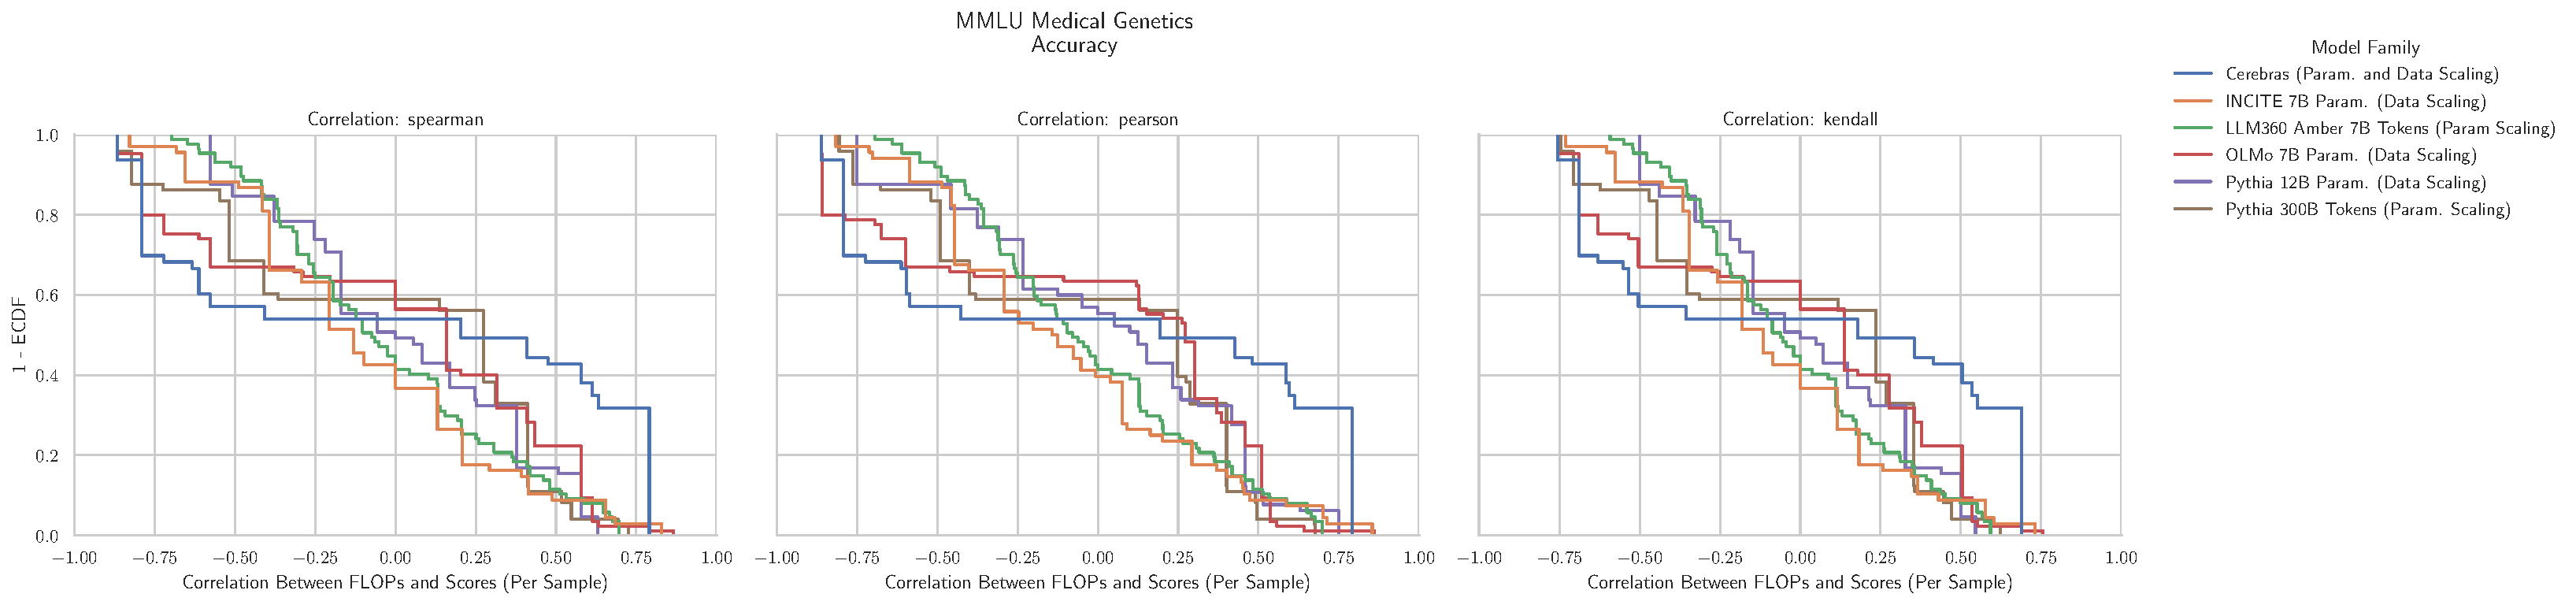
\includegraphics[width=\textwidth]{figures/correlations_between_scores_and_compute/correlation_distributions/mmlu_medical_genetics/mmlu_medical_genetics_acc_ecdf_vs_correlation_score_by_modelfamily_split_correlation_metric.pdf}
    \caption{\textbf{MMLU Medical Genetics: Downstream performance is computed via a sequence of transformations that deteriorate correlations between scores and pretraining compute.}}
    \label{app:fig:compute_score_distribution_mmlu_medical_genetics}
\end{figure}


\clearpage
\subsection{NLP Benchmark: MMLU Miscellaneous \cite{hendrycks2020mmlu}}

\begin{figure}[h!]
    \centering
    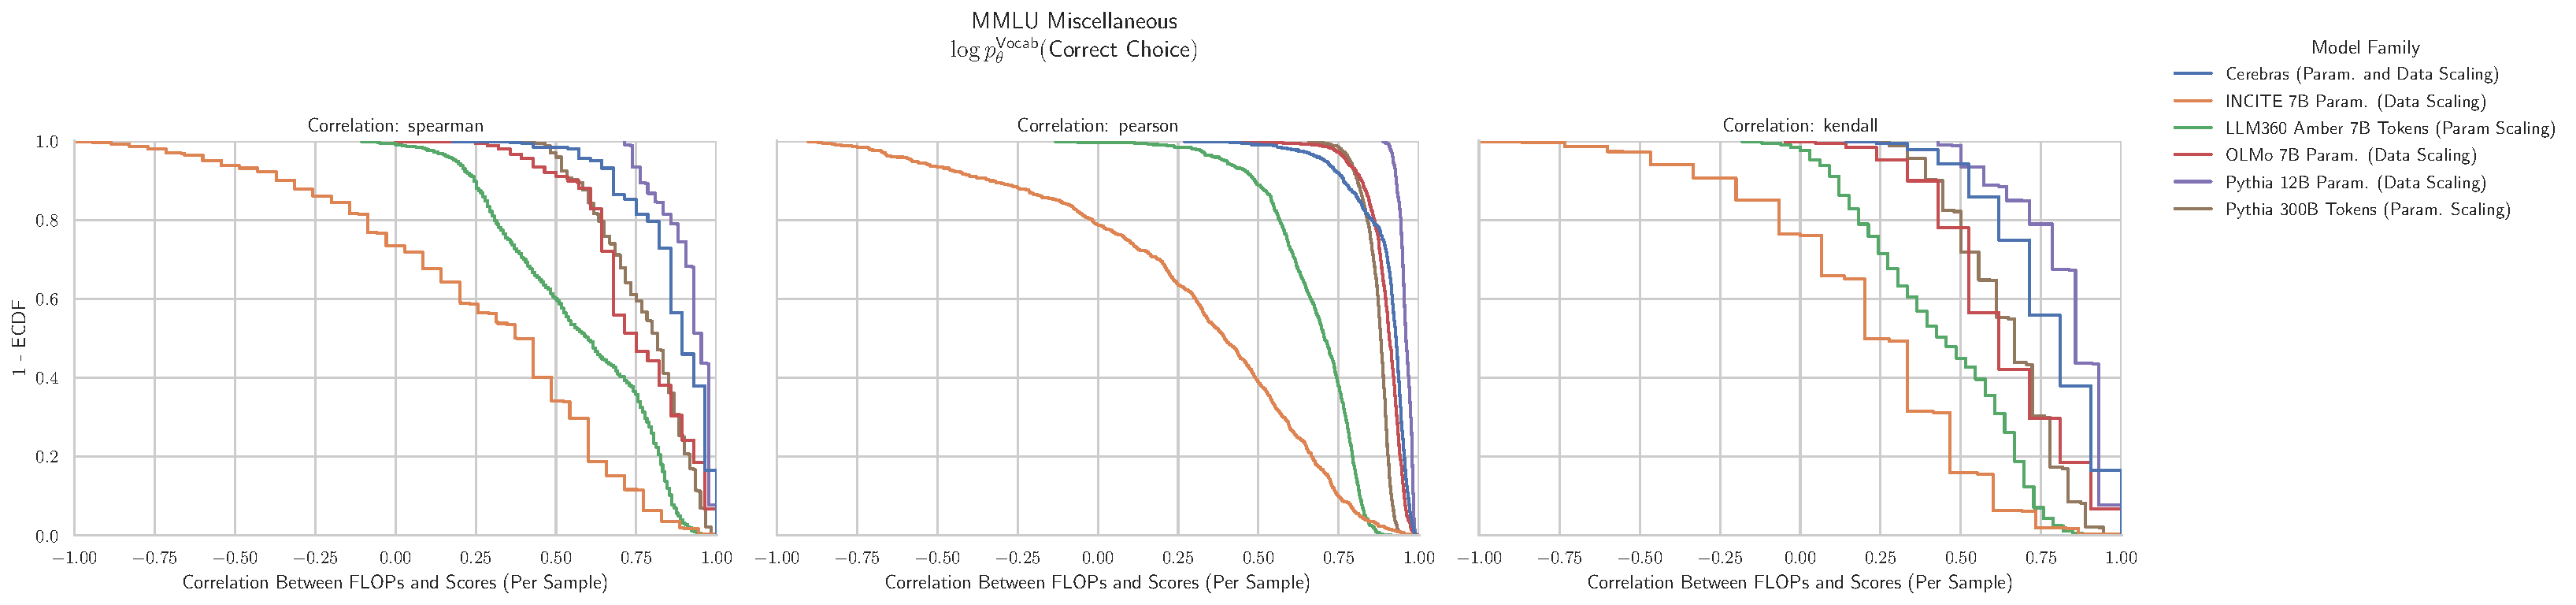
\includegraphics[width=\textwidth]{figures/correlations_between_scores_and_compute/correlation_distributions/mmlu_miscellaneous/mmlu_miscellaneous_log_likelihood_correct_ecdf_vs_correlation_score_by_modelfamily_split_correlation_metric.pdf}
    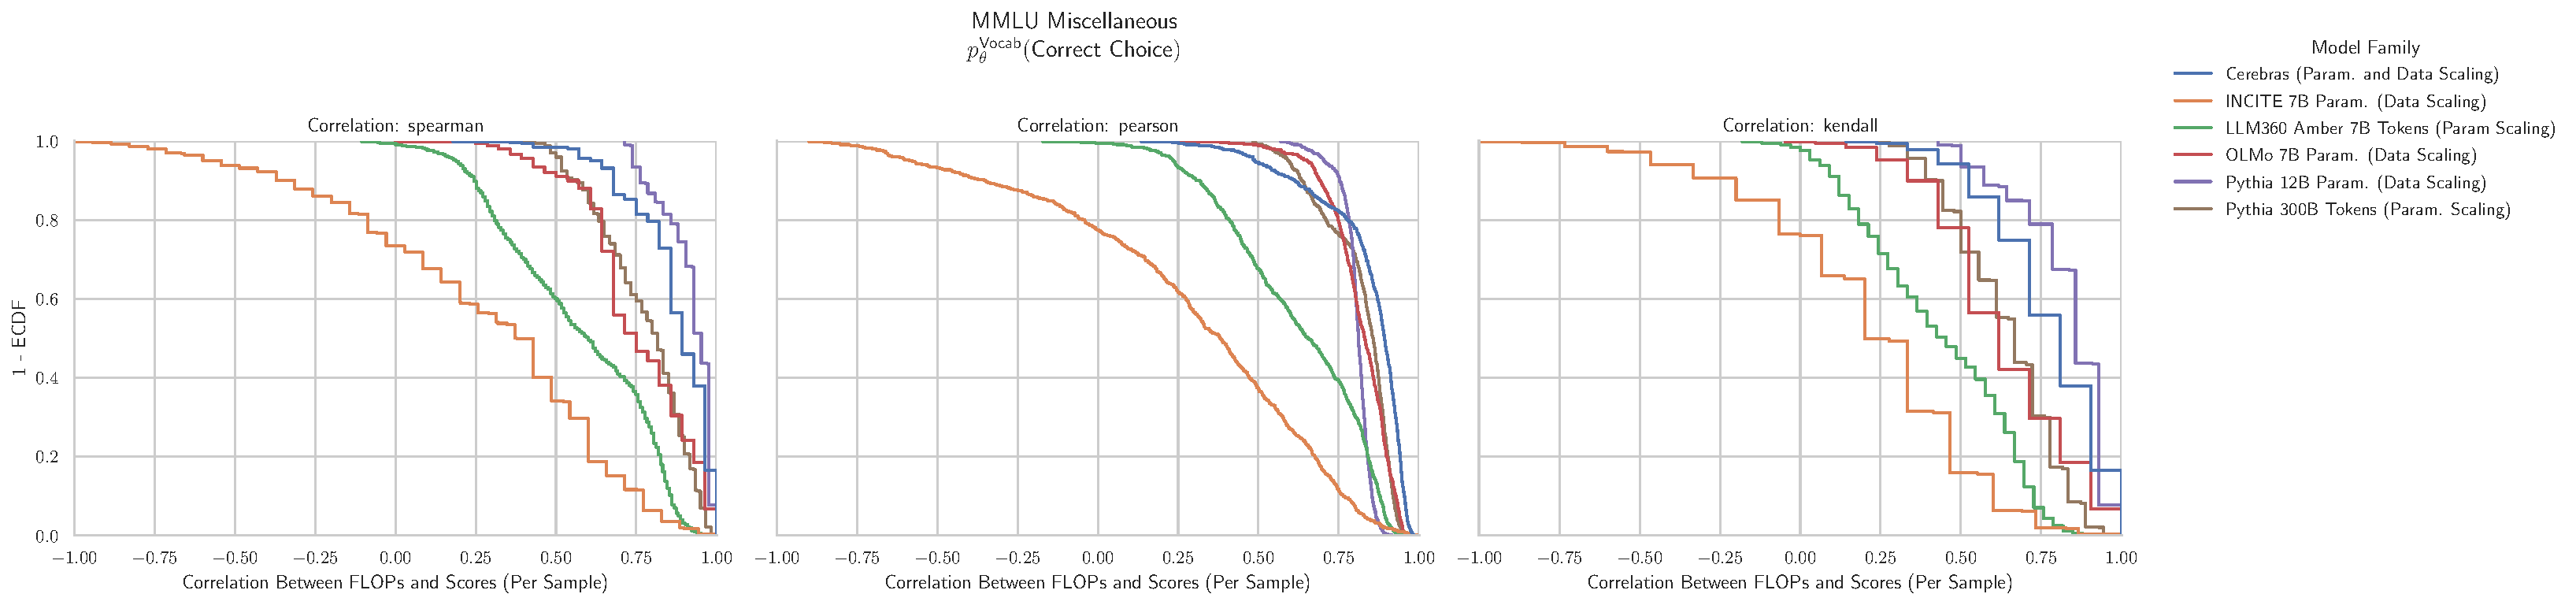
\includegraphics[width=\textwidth]{figures/correlations_between_scores_and_compute/correlation_distributions/mmlu_miscellaneous/mmlu_miscellaneous_prob_correct_vocab_ecdf_vs_correlation_score_by_modelfamily_split_correlation_metric.pdf}
    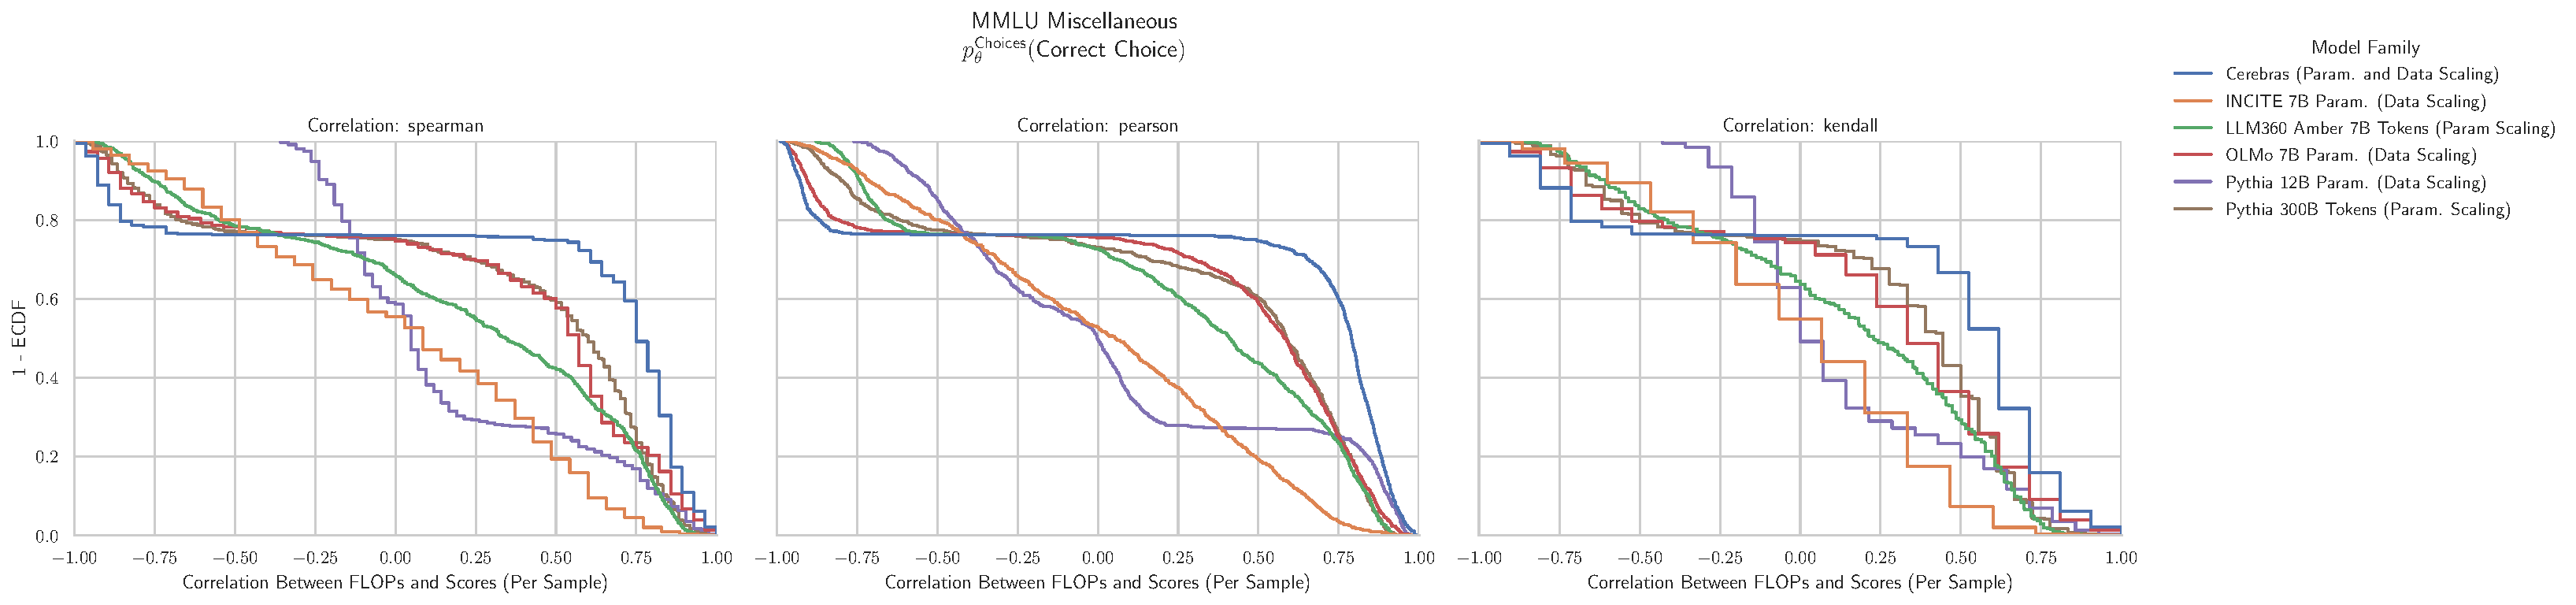
\includegraphics[width=\textwidth]{figures/correlations_between_scores_and_compute/correlation_distributions/mmlu_miscellaneous/mmlu_miscellaneous_prob_correct_choices_ecdf_vs_correlation_score_by_modelfamily_split_correlation_metric.pdf}
    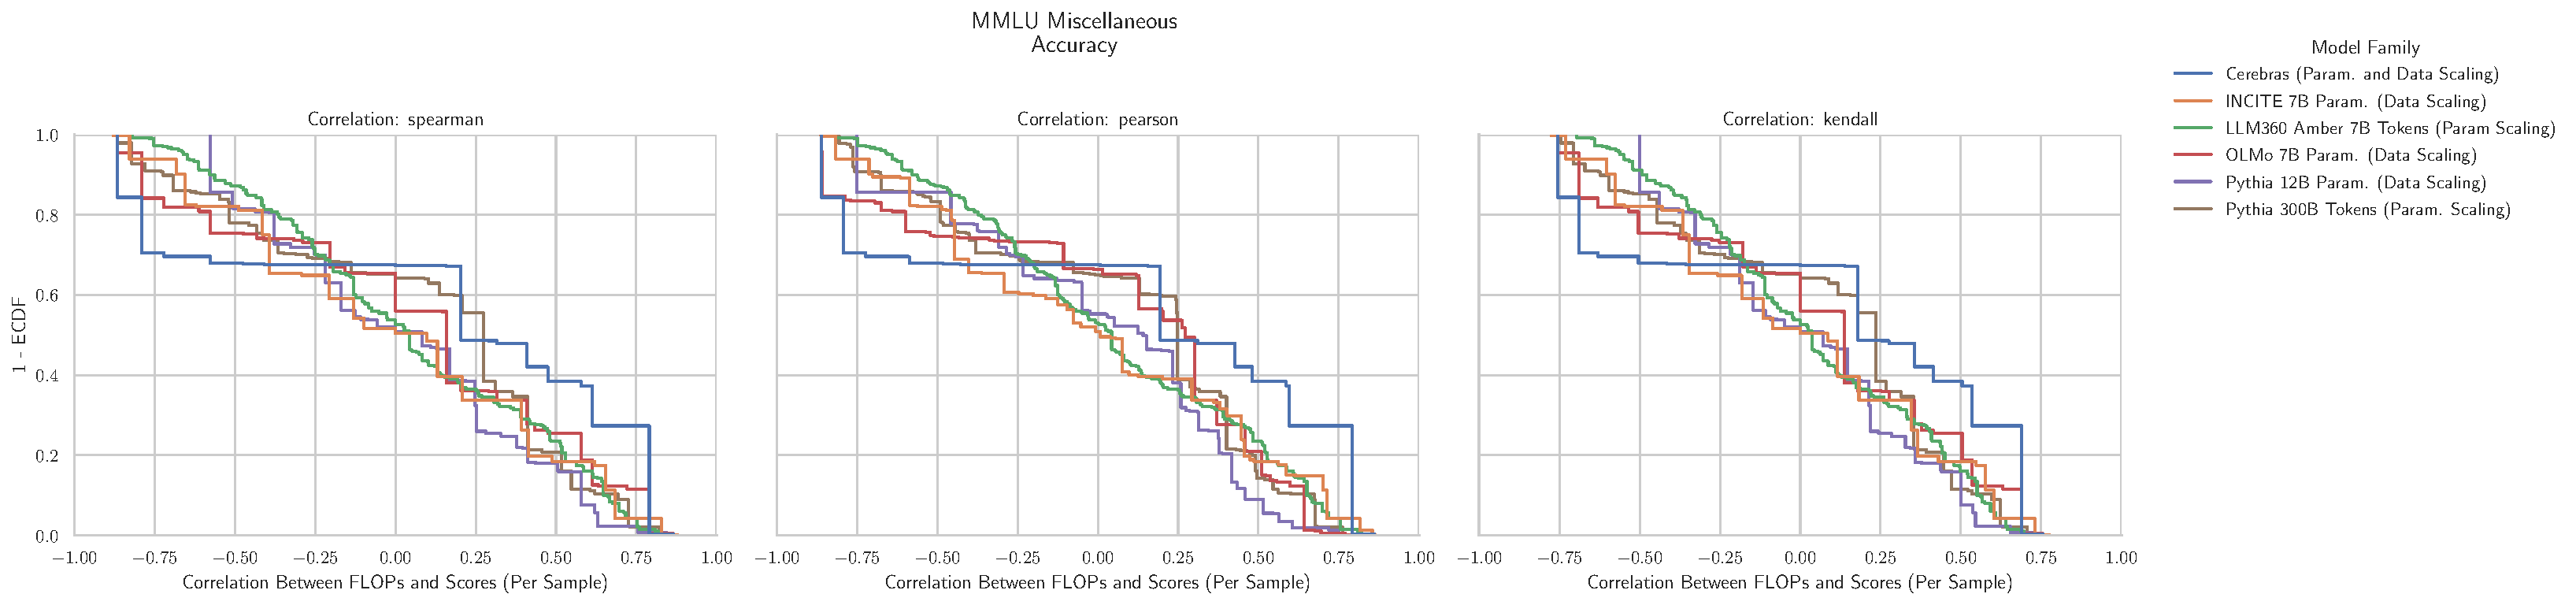
\includegraphics[width=\textwidth]{figures/correlations_between_scores_and_compute/correlation_distributions/mmlu_miscellaneous/mmlu_miscellaneous_acc_ecdf_vs_correlation_score_by_modelfamily_split_correlation_metric.pdf}
    \caption{\textbf{MMLU Miscellaneous: Downstream performance is computed via a sequence of transformations that deteriorate correlations between scores and pretraining compute.}}
    \label{app:fig:compute_score_distribution_mmlu_miscellaneous}
\end{figure}

\clearpage
\subsection{NLP Benchmark: MMLU Moral Disputes \cite{hendrycks2020mmlu}}

\begin{figure}[h!]
    \centering
    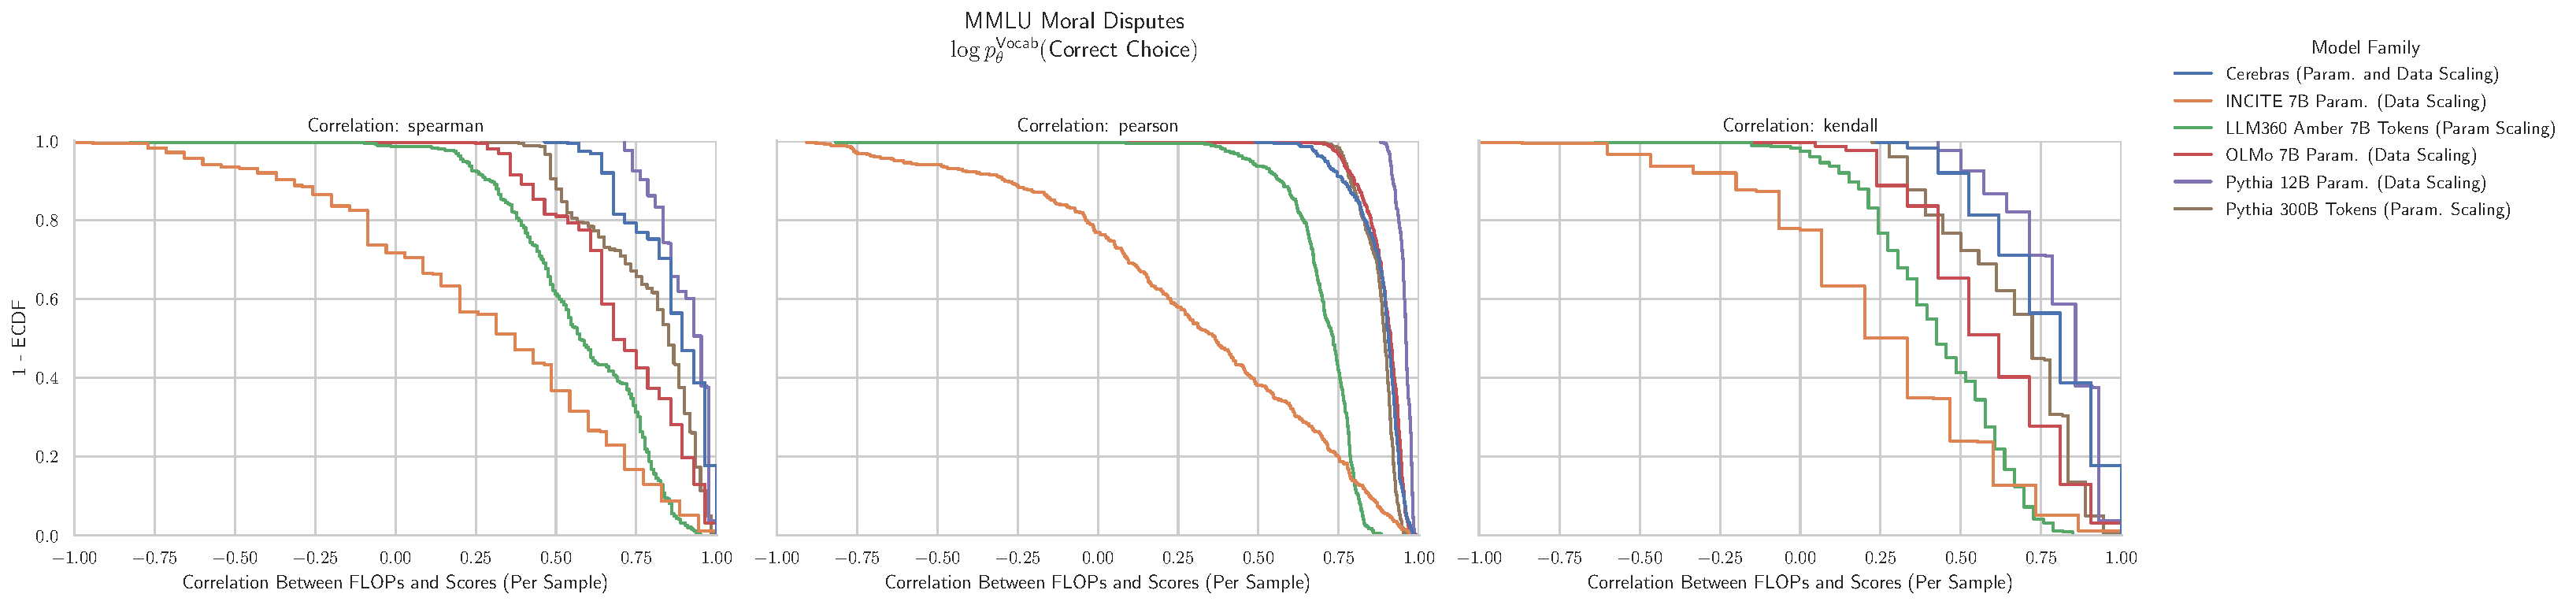
\includegraphics[width=\textwidth]{figures/correlations_between_scores_and_compute/correlation_distributions/mmlu_moral_disputes/mmlu_moral_disputes_log_likelihood_correct_ecdf_vs_correlation_score_by_modelfamily_split_correlation_metric.pdf}
    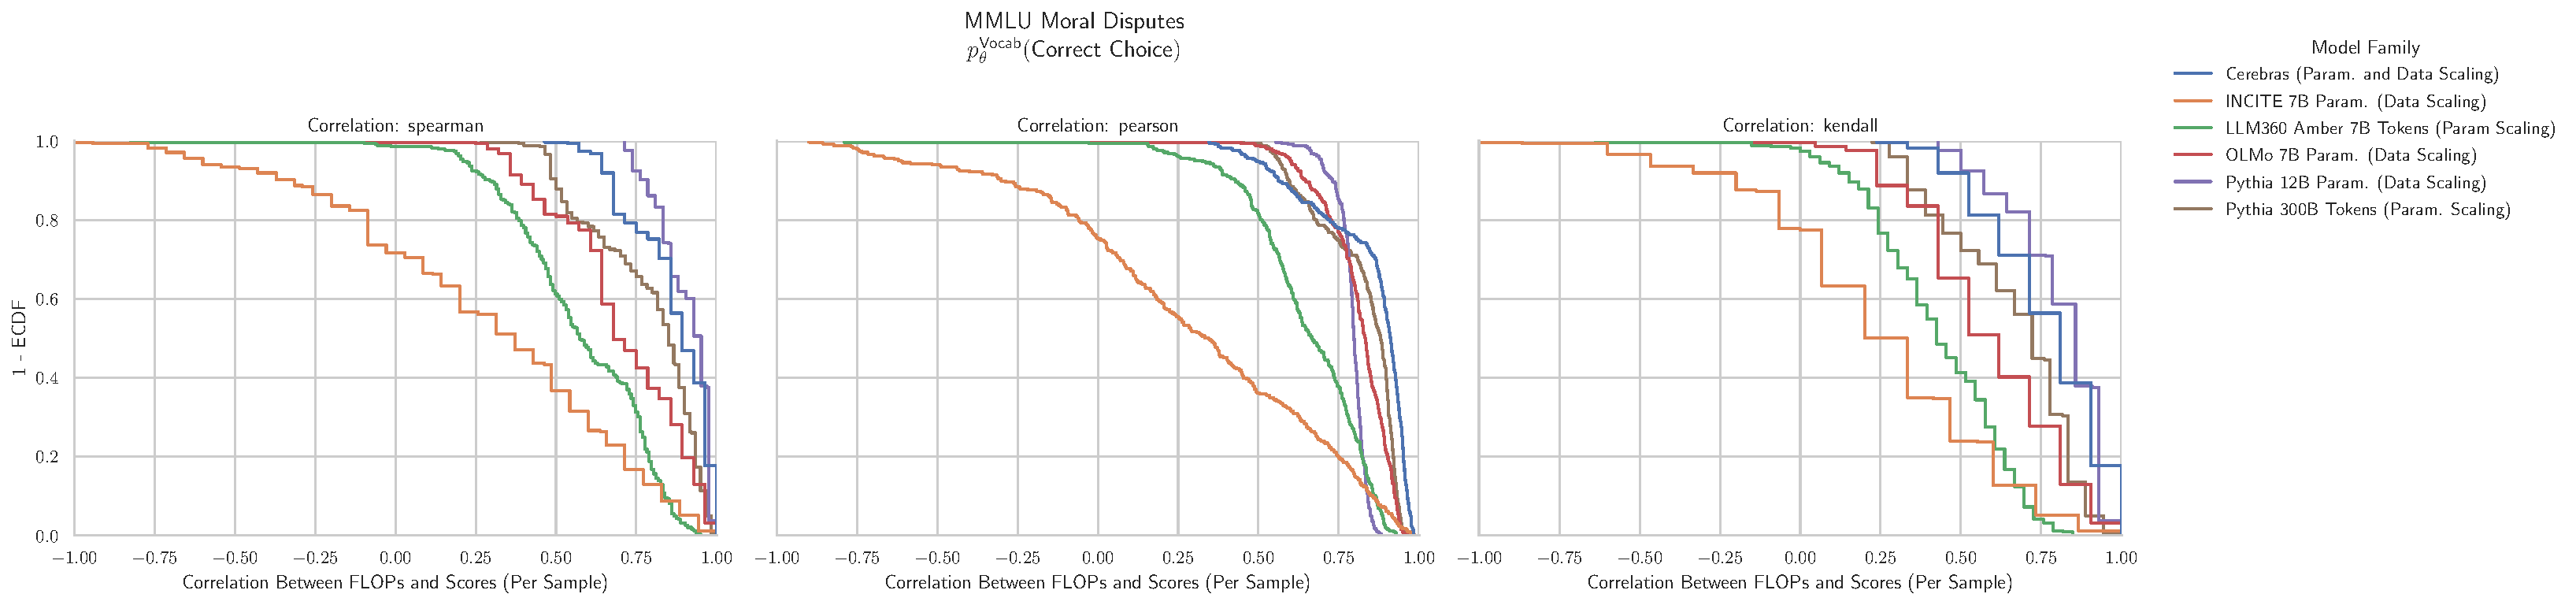
\includegraphics[width=\textwidth]{figures/correlations_between_scores_and_compute/correlation_distributions/mmlu_moral_disputes/mmlu_moral_disputes_prob_correct_vocab_ecdf_vs_correlation_score_by_modelfamily_split_correlation_metric.pdf}
    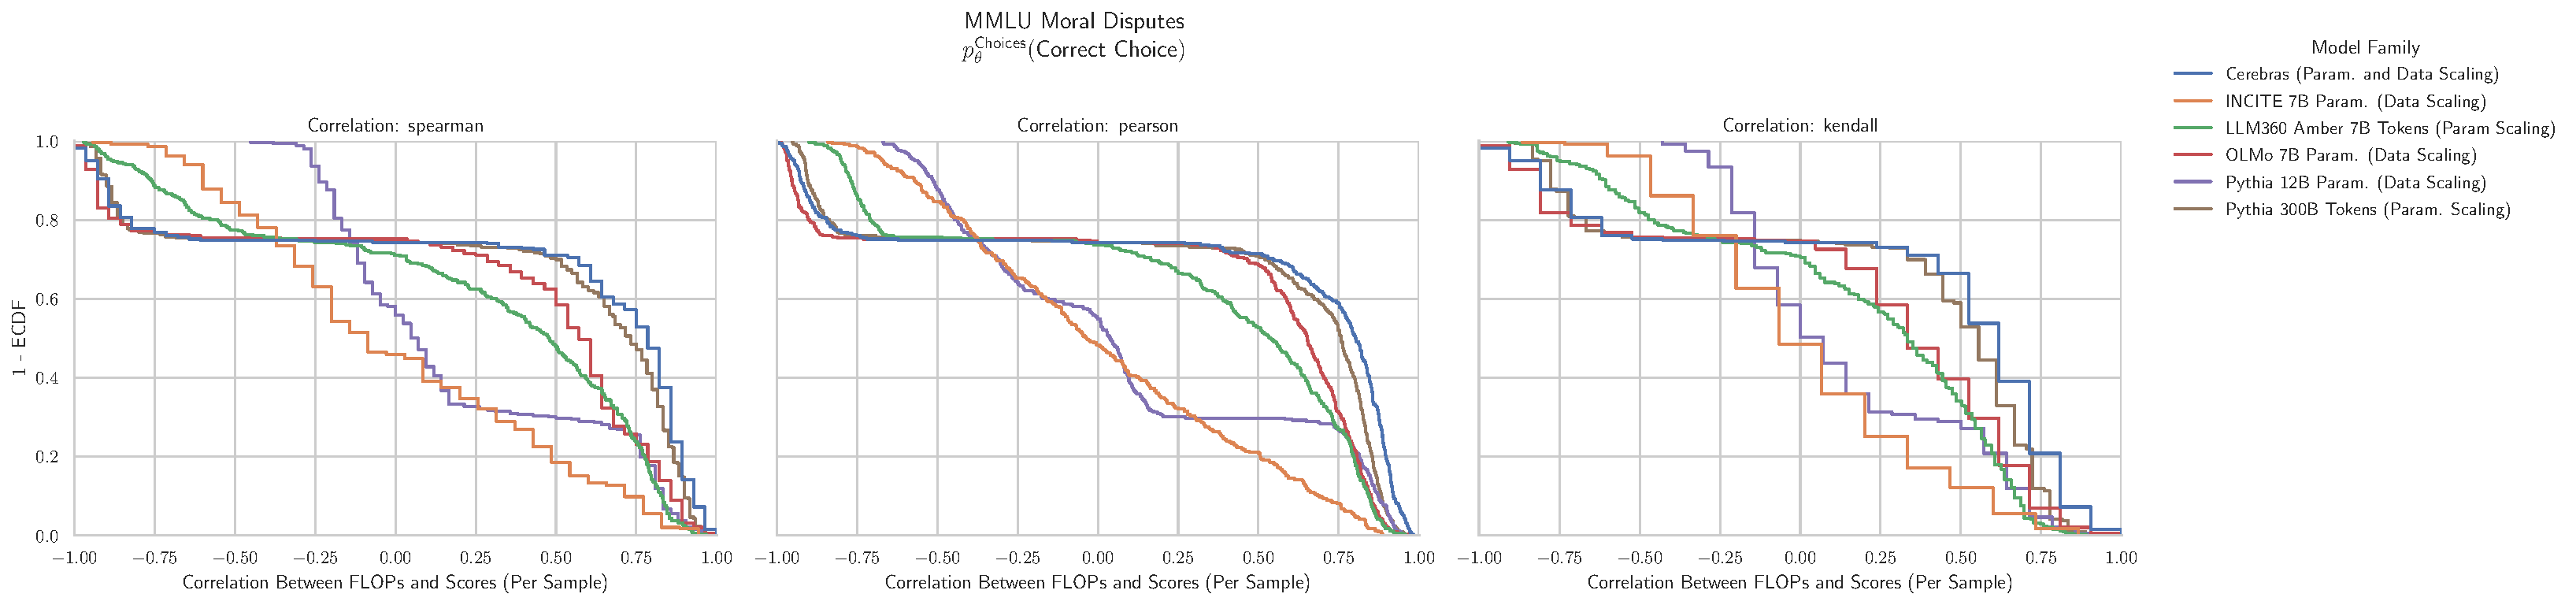
\includegraphics[width=\textwidth]{figures/correlations_between_scores_and_compute/correlation_distributions/mmlu_moral_disputes/mmlu_moral_disputes_prob_correct_choices_ecdf_vs_correlation_score_by_modelfamily_split_correlation_metric.pdf}
    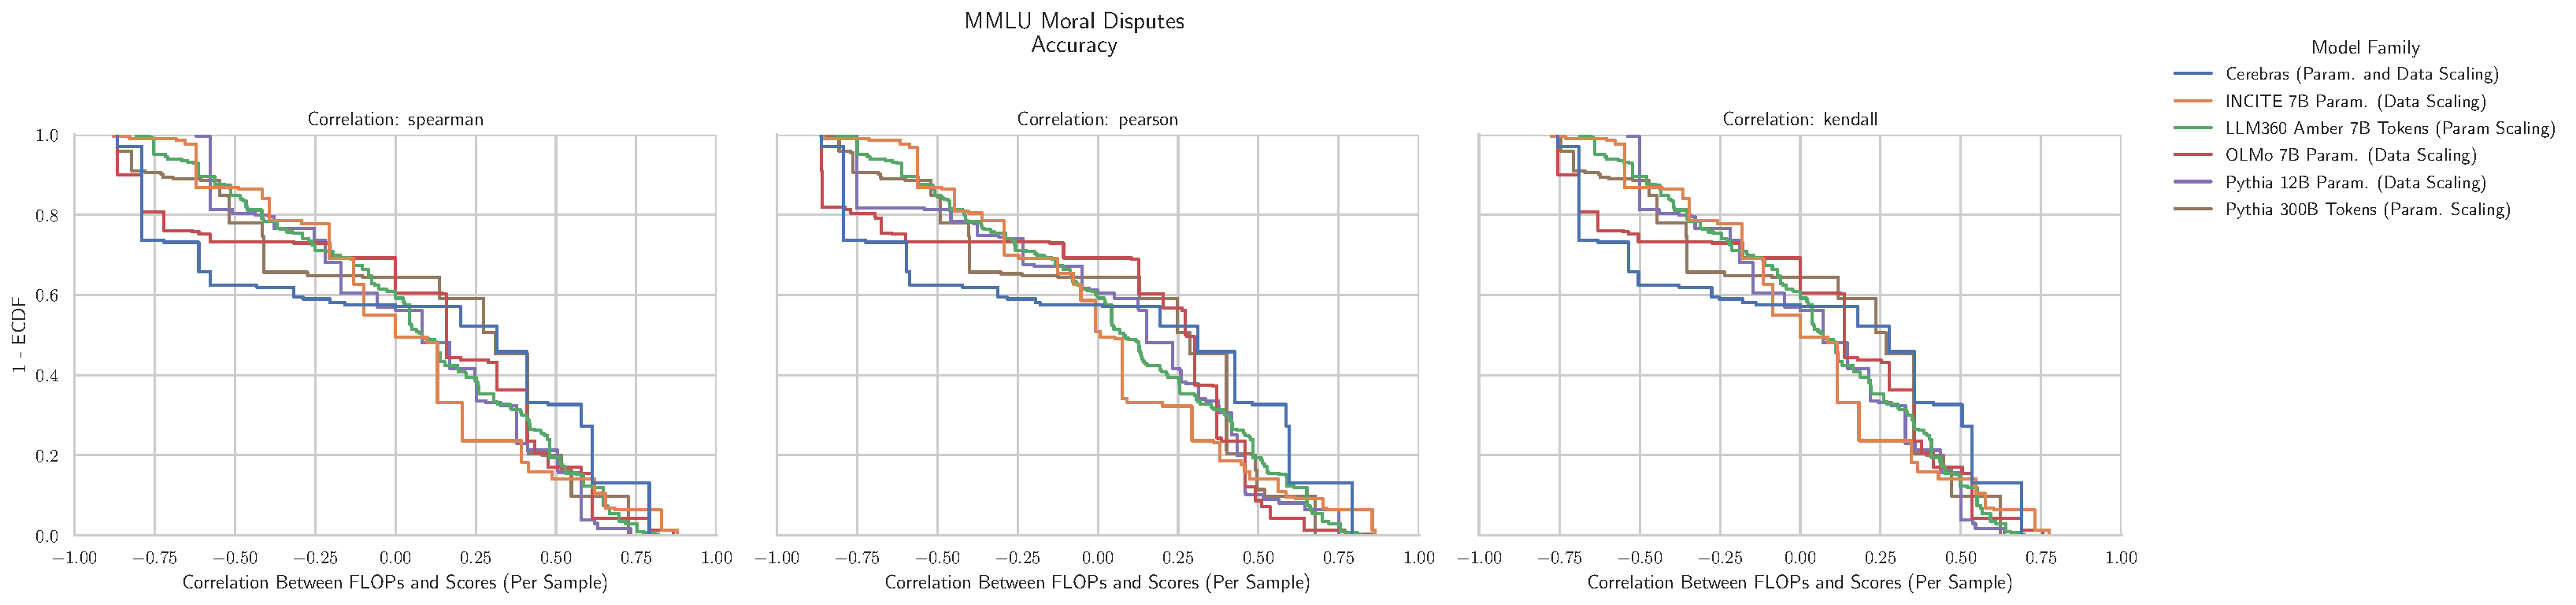
\includegraphics[width=\textwidth]{figures/correlations_between_scores_and_compute/correlation_distributions/mmlu_moral_disputes/mmlu_moral_disputes_acc_ecdf_vs_correlation_score_by_modelfamily_split_correlation_metric.pdf}
    \caption{\textbf{MMLU Moral Disputes: Downstream performance is computed via a sequence of transformations that deteriorate correlations between scores and pretraining compute.}}
    \label{app:fig:compute_score_distribution_mmlu_moral_disputes}
\end{figure}

\clearpage
\subsection{NLP Benchmark: MMLU Moral Scenarios \cite{hendrycks2020mmlu}}

\begin{figure}[h!]
    \centering
    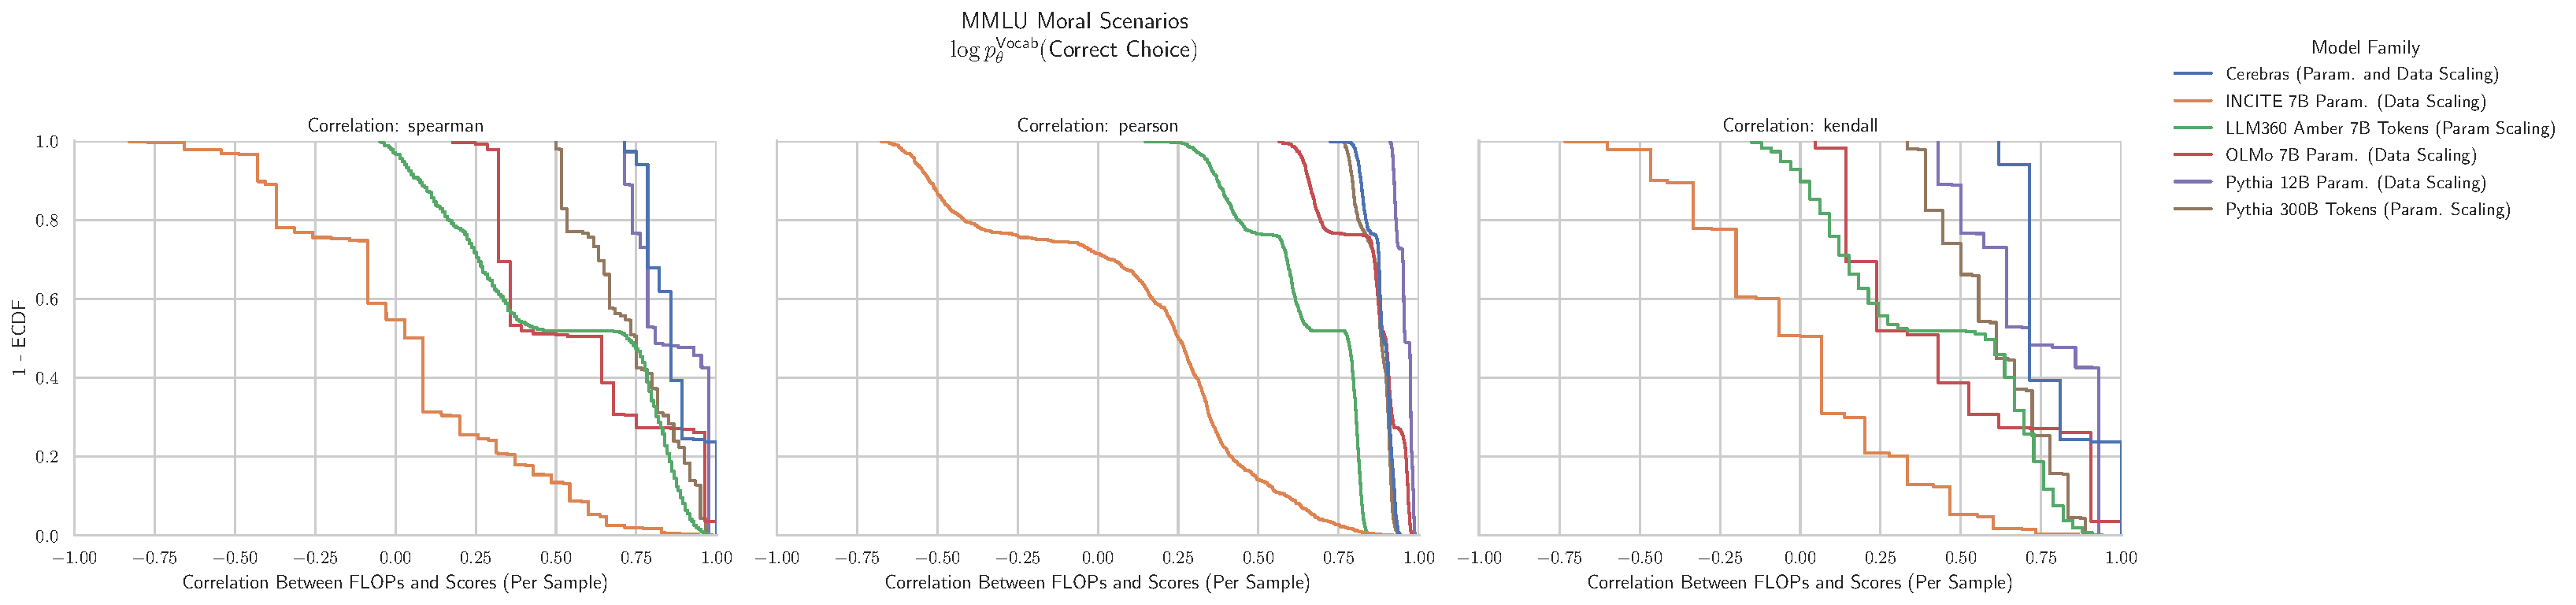
\includegraphics[width=\textwidth]{figures/correlations_between_scores_and_compute/correlation_distributions/mmlu_moral_scenarios/mmlu_moral_scenarios_log_likelihood_correct_ecdf_vs_correlation_score_by_modelfamily_split_correlation_metric.pdf}
    \includegraphics[width=\textwidth]{figures/correlations_between_scores_and_compute/correlation_distributions/mmlu_moral_scenarios/mmlu_moral_scenarios_prob_correct_vocab_ecdf_vs_correlation_score_by_modelfamily_split_correlation_metric.pdf}
    \includegraphics[width=\textwidth]{figures/correlations_between_scores_and_compute/correlation_distributions/mmlu_moral_scenarios/mmlu_moral_scenarios_prob_correct_choices_ecdf_vs_correlation_score_by_modelfamily_split_correlation_metric.pdf}
    \includegraphics[width=\textwidth]{figures/correlations_between_scores_and_compute/correlation_distributions/mmlu_moral_scenarios/mmlu_moral_scenarios_acc_ecdf_vs_correlation_score_by_modelfamily_split_correlation_metric.pdf}
    \caption{\textbf{MMLU Moral Scenarios: Downstream performance is computed via a sequence of transformations that deteriorate correlations between scores and pretraining compute.}}
    \label{app:fig:compute_score_distribution_mmlu_moral_scenarios}
\end{figure}

\clearpage
\subsection{NLP Benchmark: MMLU Nutrition \cite{hendrycks2020mmlu}}

\begin{figure}[h!]
    \centering
    \includegraphics[width=\textwidth]{figures/correlations_between_scores_and_compute/correlation_distributions/mmlu_nutrition/mmlu_nutrition_log_likelihood_correct_ecdf_vs_correlation_score_by_modelfamily_split_correlation_metric.pdf}
    \includegraphics[width=\textwidth]{figures/correlations_between_scores_and_compute/correlation_distributions/mmlu_nutrition/mmlu_nutrition_prob_correct_vocab_ecdf_vs_correlation_score_by_modelfamily_split_correlation_metric.pdf}
    \includegraphics[width=\textwidth]{figures/correlations_between_scores_and_compute/correlation_distributions/mmlu_nutrition/mmlu_nutrition_prob_correct_choices_ecdf_vs_correlation_score_by_modelfamily_split_correlation_metric.pdf}
    \includegraphics[width=\textwidth]{figures/correlations_between_scores_and_compute/correlation_distributions/mmlu_nutrition/mmlu_nutrition_acc_ecdf_vs_correlation_score_by_modelfamily_split_correlation_metric.pdf}
    \caption{\textbf{MMLU Nutrition: Downstream performance is computed via a sequence of transformations that deteriorate correlations between scores and pretraining compute.}}
    \label{app:fig:compute_score_distribution_mmlu_nutrition}
\end{figure}

\clearpage
\subsection{NLP Benchmark: MMLU Philosophy \cite{hendrycks2020mmlu}}

\begin{figure}[h!]
    \centering
    \includegraphics[width=\textwidth]{figures/correlations_between_scores_and_compute/correlation_distributions/mmlu_philosophy/mmlu_philosophy_log_likelihood_correct_ecdf_vs_correlation_score_by_modelfamily_split_correlation_metric.pdf}
    \includegraphics[width=\textwidth]{figures/correlations_between_scores_and_compute/correlation_distributions/mmlu_philosophy/mmlu_philosophy_prob_correct_vocab_ecdf_vs_correlation_score_by_modelfamily_split_correlation_metric.pdf}
    \includegraphics[width=\textwidth]{figures/correlations_between_scores_and_compute/correlation_distributions/mmlu_philosophy/mmlu_philosophy_prob_correct_choices_ecdf_vs_correlation_score_by_modelfamily_split_correlation_metric.pdf}
    \includegraphics[width=\textwidth]{figures/correlations_between_scores_and_compute/correlation_distributions/mmlu_philosophy/mmlu_philosophy_acc_ecdf_vs_correlation_score_by_modelfamily_split_correlation_metric.pdf}
    \caption{\textbf{MMLU Philosophy: Downstream performance is computed via a sequence of transformations that deteriorate correlations between scores and pretraining compute.}}
    \label{app:fig:compute_score_distribution_mmlu_philosophy}
\end{figure}

\clearpage
\subsection{NLP Benchmark: MMLU Prehistory \cite{hendrycks2020mmlu}}

\begin{figure}[h!]
    \centering
    \includegraphics[width=\textwidth]{figures/correlations_between_scores_and_compute/correlation_distributions/mmlu_prehistory/mmlu_prehistory_log_likelihood_correct_ecdf_vs_correlation_score_by_modelfamily_split_correlation_metric.pdf}
    \includegraphics[width=\textwidth]{figures/correlations_between_scores_and_compute/correlation_distributions/mmlu_prehistory/mmlu_prehistory_prob_correct_vocab_ecdf_vs_correlation_score_by_modelfamily_split_correlation_metric.pdf}
    \includegraphics[width=\textwidth]{figures/correlations_between_scores_and_compute/correlation_distributions/mmlu_prehistory/mmlu_prehistory_prob_correct_choices_ecdf_vs_correlation_score_by_modelfamily_split_correlation_metric.pdf}
    \includegraphics[width=\textwidth]{figures/correlations_between_scores_and_compute/correlation_distributions/mmlu_prehistory/mmlu_prehistory_acc_ecdf_vs_correlation_score_by_modelfamily_split_correlation_metric.pdf}
    \caption{\textbf{MMLU Prehistory: Downstream performance is computed via a sequence of transformations that deteriorate correlations between scores and pretraining compute.}}
    \label{app:fig:compute_score_distribution_mmlu_prehistory}
\end{figure}

\clearpage
\subsection{NLP Benchmark: MMLU Professional Accounting \cite{hendrycks2020mmlu}}

\begin{figure}[h!]
    \centering
    \includegraphics[width=\textwidth]{figures/correlations_between_scores_and_compute/correlation_distributions/mmlu_professional_accounting/mmlu_professional_accounting_log_likelihood_correct_ecdf_vs_correlation_score_by_modelfamily_split_correlation_metric.pdf}
    \includegraphics[width=\textwidth]{figures/correlations_between_scores_and_compute/correlation_distributions/mmlu_professional_accounting/mmlu_professional_accounting_prob_correct_vocab_ecdf_vs_correlation_score_by_modelfamily_split_correlation_metric.pdf}
    \includegraphics[width=\textwidth]{figures/correlations_between_scores_and_compute/correlation_distributions/mmlu_professional_accounting/mmlu_professional_accounting_prob_correct_choices_ecdf_vs_correlation_score_by_modelfamily_split_correlation_metric.pdf}
    \includegraphics[width=\textwidth]{figures/correlations_between_scores_and_compute/correlation_distributions/mmlu_professional_accounting/mmlu_professional_accounting_acc_ecdf_vs_correlation_score_by_modelfamily_split_correlation_metric.pdf}
    \caption{\textbf{MMLU Professional Accounting: Downstream performance is computed via a sequence of transformations that deteriorate correlations between scores and pretraining compute.}}
    \label{app:fig:compute_score_distribution_mmlu_professional_accounting}
\end{figure}

\clearpage
\subsection{NLP Benchmark: MMLU Professional Law \cite{hendrycks2020mmlu}}

\begin{figure}[h!]
    \centering
    \includegraphics[width=\textwidth]{figures/correlations_between_scores_and_compute/correlation_distributions/mmlu_professional_law/mmlu_professional_law_log_likelihood_correct_ecdf_vs_correlation_score_by_modelfamily_split_correlation_metric.pdf}
    \includegraphics[width=\textwidth]{figures/correlations_between_scores_and_compute/correlation_distributions/mmlu_professional_law/mmlu_professional_law_prob_correct_vocab_ecdf_vs_correlation_score_by_modelfamily_split_correlation_metric.pdf}
    \includegraphics[width=\textwidth]{figures/correlations_between_scores_and_compute/correlation_distributions/mmlu_professional_law/mmlu_professional_law_prob_correct_choices_ecdf_vs_correlation_score_by_modelfamily_split_correlation_metric.pdf}
    \includegraphics[width=\textwidth]{figures/correlations_between_scores_and_compute/correlation_distributions/mmlu_professional_law/mmlu_professional_law_acc_ecdf_vs_correlation_score_by_modelfamily_split_correlation_metric.pdf}
    \caption{\textbf{MMLU Professional Law: Downstream performance is computed via a sequence of transformations that deteriorate correlations between scores and pretraining compute.}}
    \label{app:fig:compute_score_distribution_mmlu_professional_law}
\end{figure}

\clearpage
\subsection{NLP Benchmark: MMLU Professional Medicine \cite{hendrycks2020mmlu}}

\begin{figure}[h!]
    \centering
    \includegraphics[width=\textwidth]{figures/correlations_between_scores_and_compute/correlation_distributions/mmlu_professional_medicine/mmlu_professional_medicine_log_likelihood_correct_ecdf_vs_correlation_score_by_modelfamily_split_correlation_metric.pdf}
    \includegraphics[width=\textwidth]{figures/correlations_between_scores_and_compute/correlation_distributions/mmlu_professional_medicine/mmlu_professional_medicine_prob_correct_vocab_ecdf_vs_correlation_score_by_modelfamily_split_correlation_metric.pdf}
    \includegraphics[width=\textwidth]{figures/correlations_between_scores_and_compute/correlation_distributions/mmlu_professional_medicine/mmlu_professional_medicine_prob_correct_choices_ecdf_vs_correlation_score_by_modelfamily_split_correlation_metric.pdf}
    \includegraphics[width=\textwidth]{figures/correlations_between_scores_and_compute/correlation_distributions/mmlu_professional_medicine/mmlu_professional_medicine_acc_ecdf_vs_correlation_score_by_modelfamily_split_correlation_metric.pdf}
    \caption{\textbf{MMLU Professional Medicine: Downstream performance is computed via a sequence of transformations that deteriorate correlations between scores and pretraining compute.}}
    \label{app:fig:compute_score_distribution_mmlu_professional_medicine}
\end{figure}

\clearpage
\subsection{NLP Benchmark: MMLU Professional Psychology \cite{hendrycks2020mmlu}}

\begin{figure}[h!]
    \centering
    \includegraphics[width=\textwidth]{figures/correlations_between_scores_and_compute/correlation_distributions/mmlu_professional_psychology/mmlu_professional_psychology_log_likelihood_correct_ecdf_vs_correlation_score_by_modelfamily_split_correlation_metric.pdf}
    \includegraphics[width=\textwidth]{figures/correlations_between_scores_and_compute/correlation_distributions/mmlu_professional_psychology/mmlu_professional_psychology_prob_correct_vocab_ecdf_vs_correlation_score_by_modelfamily_split_correlation_metric.pdf}
    \includegraphics[width=\textwidth]{figures/correlations_between_scores_and_compute/correlation_distributions/mmlu_professional_psychology/mmlu_professional_psychology_prob_correct_choices_ecdf_vs_correlation_score_by_modelfamily_split_correlation_metric.pdf}
    \includegraphics[width=\textwidth]{figures/correlations_between_scores_and_compute/correlation_distributions/mmlu_professional_psychology/mmlu_professional_psychology_acc_ecdf_vs_correlation_score_by_modelfamily_split_correlation_metric.pdf}
    \caption{\textbf{MMLU Professional Psychology: Downstream performance is computed via a sequence of transformations that deteriorate correlations between scores and pretraining compute.}}
    \label{app:fig:compute_score_distribution_mmlu_professional_psychology}
\end{figure}

\clearpage
\subsection{NLP Benchmark: MMLU Public Relations \cite{hendrycks2020mmlu}}

\begin{figure}[h!]
    \centering
    \includegraphics[width=\textwidth]{figures/correlations_between_scores_and_compute/correlation_distributions/mmlu_public_relations/mmlu_public_relations_log_likelihood_correct_ecdf_vs_correlation_score_by_modelfamily_split_correlation_metric.pdf}
    \includegraphics[width=\textwidth]{figures/correlations_between_scores_and_compute/correlation_distributions/mmlu_public_relations/mmlu_public_relations_prob_correct_vocab_ecdf_vs_correlation_score_by_modelfamily_split_correlation_metric.pdf}
    \includegraphics[width=\textwidth]{figures/correlations_between_scores_and_compute/correlation_distributions/mmlu_public_relations/mmlu_public_relations_prob_correct_choices_ecdf_vs_correlation_score_by_modelfamily_split_correlation_metric.pdf}
    \includegraphics[width=\textwidth]{figures/correlations_between_scores_and_compute/correlation_distributions/mmlu_public_relations/mmlu_public_relations_acc_ecdf_vs_correlation_score_by_modelfamily_split_correlation_metric.pdf}
    \caption{\textbf{MMLU Public Relations: Downstream performance is computed via a sequence of transformations that deteriorate correlations between scores and pretraining compute.}}
    \label{app:fig:compute_score_distribution_mmlu_public_relations}
\end{figure}


\clearpage
\subsection{NLP Benchmark: MMLU Security Studies \cite{hendrycks2020mmlu}}

\begin{figure}[h!]
    \centering
    \includegraphics[width=\textwidth]{figures/correlations_between_scores_and_compute/correlation_distributions/mmlu_security_studies/mmlu_security_studies_log_likelihood_correct_ecdf_vs_correlation_score_by_modelfamily_split_correlation_metric.pdf}
    \includegraphics[width=\textwidth]{figures/correlations_between_scores_and_compute/correlation_distributions/mmlu_security_studies/mmlu_security_studies_prob_correct_vocab_ecdf_vs_correlation_score_by_modelfamily_split_correlation_metric.pdf}
    \includegraphics[width=\textwidth]{figures/correlations_between_scores_and_compute/correlation_distributions/mmlu_security_studies/mmlu_security_studies_prob_correct_choices_ecdf_vs_correlation_score_by_modelfamily_split_correlation_metric.pdf}
    \includegraphics[width=\textwidth]{figures/correlations_between_scores_and_compute/correlation_distributions/mmlu_security_studies/mmlu_security_studies_acc_ecdf_vs_correlation_score_by_modelfamily_split_correlation_metric.pdf}
    \caption{\textbf{MMLU Security Studies: Downstream performance is computed via a sequence of transformations that deteriorate correlations between scores and pretraining compute.}}
    \label{app:fig:compute_score_distribution_mmlu_security_studies}
\end{figure}


\clearpage
\subsection{NLP Benchmark: MMLU Sociology \cite{hendrycks2020mmlu}}

\begin{figure}[h!]
    \centering
    \includegraphics[width=\textwidth]{figures/correlations_between_scores_and_compute/correlation_distributions/mmlu_sociology/mmlu_sociology_log_likelihood_correct_ecdf_vs_correlation_score_by_modelfamily_split_correlation_metric.pdf}
    \includegraphics[width=\textwidth]{figures/correlations_between_scores_and_compute/correlation_distributions/mmlu_sociology/mmlu_sociology_prob_correct_vocab_ecdf_vs_correlation_score_by_modelfamily_split_correlation_metric.pdf}
    \includegraphics[width=\textwidth]{figures/correlations_between_scores_and_compute/correlation_distributions/mmlu_sociology/mmlu_sociology_prob_correct_choices_ecdf_vs_correlation_score_by_modelfamily_split_correlation_metric.pdf}
    \includegraphics[width=\textwidth]{figures/correlations_between_scores_and_compute/correlation_distributions/mmlu_sociology/mmlu_sociology_acc_ecdf_vs_correlation_score_by_modelfamily_split_correlation_metric.pdf}
    \caption{\textbf{MMLU Sociology: Downstream performance is computed via a sequence of transformations that deteriorate correlations between scores and pretraining compute.}}
    \label{app:fig:compute_score_distribution_mmlu_sociology}
\end{figure}


\clearpage
\subsection{NLP Benchmark: MMLU US Foreign Policy \cite{hendrycks2020mmlu}}

\begin{figure}[h!]
    \centering
    \includegraphics[width=\textwidth]{figures/correlations_between_scores_and_compute/correlation_distributions/mmlu_us_foreign_policy/mmlu_us_foreign_policy_log_likelihood_correct_ecdf_vs_correlation_score_by_modelfamily_split_correlation_metric.pdf}
    \includegraphics[width=\textwidth]{figures/correlations_between_scores_and_compute/correlation_distributions/mmlu_us_foreign_policy/mmlu_us_foreign_policy_prob_correct_vocab_ecdf_vs_correlation_score_by_modelfamily_split_correlation_metric.pdf}
    \includegraphics[width=\textwidth]{figures/correlations_between_scores_and_compute/correlation_distributions/mmlu_us_foreign_policy/mmlu_us_foreign_policy_prob_correct_choices_ecdf_vs_correlation_score_by_modelfamily_split_correlation_metric.pdf}
    \includegraphics[width=\textwidth]{figures/correlations_between_scores_and_compute/correlation_distributions/mmlu_us_foreign_policy/mmlu_us_foreign_policy_acc_ecdf_vs_correlation_score_by_modelfamily_split_correlation_metric.pdf}
    \caption{\textbf{MMLU US Foreign Policy: Downstream performance is computed via a sequence of transformations that deteriorate correlations between scores and pretraining compute.}}
    \label{app:fig:compute_score_distribution_mmlu_us_foreign_policy}
\end{figure}



\clearpage
\subsection{NLP Benchmark: MMLU Virology \cite{hendrycks2020mmlu}}

\begin{figure}[h!]
    \centering
    \includegraphics[width=\textwidth]{figures/correlations_between_scores_and_compute/correlation_distributions/mmlu_virology/mmlu_virology_log_likelihood_correct_ecdf_vs_correlation_score_by_modelfamily_split_correlation_metric.pdf}
    \includegraphics[width=\textwidth]{figures/correlations_between_scores_and_compute/correlation_distributions/mmlu_virology/mmlu_virology_prob_correct_vocab_ecdf_vs_correlation_score_by_modelfamily_split_correlation_metric.pdf}
    \includegraphics[width=\textwidth]{figures/correlations_between_scores_and_compute/correlation_distributions/mmlu_virology/mmlu_virology_prob_correct_choices_ecdf_vs_correlation_score_by_modelfamily_split_correlation_metric.pdf}
    \includegraphics[width=\textwidth]{figures/correlations_between_scores_and_compute/correlation_distributions/mmlu_virology/mmlu_virology_acc_ecdf_vs_correlation_score_by_modelfamily_split_correlation_metric.pdf}
    \caption{\textbf{MMLU Virology: Downstream performance is computed via a sequence of transformations that deteriorate correlations between scores and pretraining compute.}}
    \label{app:fig:compute_score_distribution_mmlu_virology}
\end{figure}


\clearpage
\subsection{NLP Benchmark: MMLU World Religions \cite{hendrycks2020mmlu}}

\begin{figure}[h!]
    \centering
    \includegraphics[width=\textwidth]{figures/correlations_between_scores_and_compute/correlation_distributions/mmlu_world_religions/mmlu_world_religions_log_likelihood_correct_ecdf_vs_correlation_score_by_modelfamily_split_correlation_metric.pdf}
    \includegraphics[width=\textwidth]{figures/correlations_between_scores_and_compute/correlation_distributions/mmlu_world_religions/mmlu_world_religions_prob_correct_vocab_ecdf_vs_correlation_score_by_modelfamily_split_correlation_metric.pdf}
    \includegraphics[width=\textwidth]{figures/correlations_between_scores_and_compute/correlation_distributions/mmlu_world_religions/mmlu_world_religions_prob_correct_choices_ecdf_vs_correlation_score_by_modelfamily_split_correlation_metric.pdf}
    \includegraphics[width=\textwidth]{figures/correlations_between_scores_and_compute/correlation_distributions/mmlu_world_religions/mmlu_world_religions_acc_ecdf_vs_correlation_score_by_modelfamily_split_correlation_metric.pdf}
    \caption{\textbf{MMLU World Religions: Downstream performance is computed via a sequence of transformations that deteriorate correlations between scores and pretraining compute.}}
    \label{app:fig:compute_score_distribution_mmlu_world_religions}
\end{figure}


\clearpage
\subsection{NLP Benchmark: OpenBookQA \cite{mihaylov2018openbookqa}}

\begin{figure}[h!]
    \centering
    \includegraphics[width=\textwidth]{figures/correlations_between_scores_and_compute/correlation_distributions/openbookqa/openbookqa_log_likelihood_correct_ecdf_vs_correlation_score_by_modelfamily_split_correlation_metric.pdf}
    \includegraphics[width=\textwidth]{figures/correlations_between_scores_and_compute/correlation_distributions/openbookqa/openbookqa_prob_correct_vocab_ecdf_vs_correlation_score_by_modelfamily_split_correlation_metric.pdf}
    \includegraphics[width=\textwidth]{figures/correlations_between_scores_and_compute/correlation_distributions/openbookqa/openbookqa_prob_correct_choices_ecdf_vs_correlation_score_by_modelfamily_split_correlation_metric.pdf}
    \includegraphics[width=\textwidth]{figures/correlations_between_scores_and_compute/correlation_distributions/openbookqa/openbookqa_acc_ecdf_vs_correlation_score_by_modelfamily_split_correlation_metric.pdf}
    \caption{\textbf{OpenBookQA: Downstream performance is computed via a sequence of transformations that deteriorate correlations between scores and pretraining compute.}}
    \label{app:fig:compute_score_distribution_openbookqa}
\end{figure}

\clearpage
\subsection{NLP Benchmark: PIQA \cite{bisk2020piqa}}

\begin{figure}[h!]
    \centering
    \includegraphics[width=\textwidth]{figures/correlations_between_scores_and_compute/correlation_distributions/piqa/piqa_log_likelihood_correct_ecdf_vs_correlation_score_by_modelfamily_split_correlation_metric.pdf}
    \includegraphics[width=\textwidth]{figures/correlations_between_scores_and_compute/correlation_distributions/piqa/piqa_prob_correct_vocab_ecdf_vs_correlation_score_by_modelfamily_split_correlation_metric.pdf}
    \includegraphics[width=\textwidth]{figures/correlations_between_scores_and_compute/correlation_distributions/piqa/piqa_prob_correct_choices_ecdf_vs_correlation_score_by_modelfamily_split_correlation_metric.pdf}
    \includegraphics[width=\textwidth]{figures/correlations_between_scores_and_compute/correlation_distributions/piqa/piqa_acc_ecdf_vs_correlation_score_by_modelfamily_split_correlation_metric.pdf}
    \caption{\textbf{PIQA: Downstream performance is computed via a sequence of transformations that deteriorate correlations between scores and pretraining compute.}}
    \label{app:fig:compute_score_distribution_piqa}
\end{figure}

\clearpage
\subsection{NLP Benchmark: RACE \cite{lai2017race}}

\begin{figure}[h!]
    \centering
    \includegraphics[width=\textwidth]{figures/correlations_between_scores_and_compute/correlation_distributions/race/race_log_likelihood_correct_ecdf_vs_correlation_score_by_modelfamily_split_correlation_metric.pdf}
    \includegraphics[width=\textwidth]{figures/correlations_between_scores_and_compute/correlation_distributions/race/race_prob_correct_vocab_ecdf_vs_correlation_score_by_modelfamily_split_correlation_metric.pdf}
    \includegraphics[width=\textwidth]{figures/correlations_between_scores_and_compute/correlation_distributions/race/race_prob_correct_choices_ecdf_vs_correlation_score_by_modelfamily_split_correlation_metric.pdf}
    \includegraphics[width=\textwidth]{figures/correlations_between_scores_and_compute/correlation_distributions/race/race_acc_ecdf_vs_correlation_score_by_modelfamily_split_correlation_metric.pdf}
    \caption{\textbf{RACE: Downstream performance is computed via a sequence of transformations that deteriorate correlations between scores and pretraining compute.}}
    \label{app:fig:compute_score_distribution_race}
\end{figure}

\clearpage
\subsection{NLP Benchmark: SciQ \cite{welbl2017sciq}}

\begin{figure}[h!]
    \centering
    \includegraphics[width=\textwidth]{figures/correlations_between_scores_and_compute/correlation_distributions/sciq/sciq_log_likelihood_correct_ecdf_vs_correlation_score_by_modelfamily_split_correlation_metric.pdf}
    \includegraphics[width=\textwidth]{figures/correlations_between_scores_and_compute/correlation_distributions/sciq/sciq_prob_correct_vocab_ecdf_vs_correlation_score_by_modelfamily_split_correlation_metric.pdf}
    \includegraphics[width=\textwidth]{figures/correlations_between_scores_and_compute/correlation_distributions/sciq/sciq_prob_correct_choices_ecdf_vs_correlation_score_by_modelfamily_split_correlation_metric.pdf}
    \includegraphics[width=\textwidth]{figures/correlations_between_scores_and_compute/correlation_distributions/sciq/sciq_acc_ecdf_vs_correlation_score_by_modelfamily_split_correlation_metric.pdf}
    \caption{\textbf{SciQ: Downstream performance is computed via a sequence of transformations that deteriorate correlations between scores and pretraining compute.}}
    \label{app:fig:compute_score_distribution_sciq}
\end{figure}

\clearpage

\subsection{NLP Benchmark: Social IQA \cite{sap2019socialiqa}}

\begin{figure}[h!]
    \centering
    \includegraphics[width=\textwidth]{figures/correlations_between_scores_and_compute/correlation_distributions/social_iqa/social_iqa_log_likelihood_correct_ecdf_vs_correlation_score_by_modelfamily_split_correlation_metric.pdf}
    \includegraphics[width=\textwidth]{figures/correlations_between_scores_and_compute/correlation_distributions/social_iqa/social_iqa_prob_correct_vocab_ecdf_vs_correlation_score_by_modelfamily_split_correlation_metric.pdf}
    \includegraphics[width=\textwidth]{figures/correlations_between_scores_and_compute/correlation_distributions/social_iqa/social_iqa_prob_correct_choices_ecdf_vs_correlation_score_by_modelfamily_split_correlation_metric.pdf}
    \includegraphics[width=\textwidth]{figures/correlations_between_scores_and_compute/correlation_distributions/social_iqa/social_iqa_acc_ecdf_vs_correlation_score_by_modelfamily_split_correlation_metric.pdf}
    \caption{\textbf{Social IQA: Downstream performance is computed via a sequence of transformations that deteriorate correlations between scores and pretraining compute.}}
    \label{app:fig:compute_score_distribution_siqa}
\end{figure}

\clearpage
\subsection{NLP Benchmark: Winogrande \cite{keisuke2019winogrande}}

\begin{figure}[h!]
    \centering
    \includegraphics[width=\textwidth]{figures/correlations_between_scores_and_compute/correlation_distributions/winogrande/winogrande_log_likelihood_correct_ecdf_vs_correlation_score_by_modelfamily_split_correlation_metric.pdf}
    \includegraphics[width=\textwidth]{figures/correlations_between_scores_and_compute/correlation_distributions/winogrande/winogrande_prob_correct_vocab_ecdf_vs_correlation_score_by_modelfamily_split_correlation_metric.pdf}
    \includegraphics[width=\textwidth]{figures/correlations_between_scores_and_compute/correlation_distributions/winogrande/winogrande_prob_correct_choices_ecdf_vs_correlation_score_by_modelfamily_split_correlation_metric.pdf}
    \includegraphics[width=\textwidth]{figures/correlations_between_scores_and_compute/correlation_distributions/winogrande/winogrande_acc_ecdf_vs_correlation_score_by_modelfamily_split_correlation_metric.pdf}
    \caption{\textbf{Social IQA: Downstream performance is computed via a sequence of transformations that deteriorate correlations between scores and pretraining compute.}}
    \label{app:fig:compute_score_distribution_winogrande}
\end{figure}


\clearpage
\subsection{NLP Benchmark: XWinograd English \cite{muennighoff2023xwinograd}}

\begin{figure}[h!]
    \centering
    \includegraphics[width=\textwidth]{figures/correlations_between_scores_and_compute/correlation_distributions/xwinograd_en/xwinograd_en_log_prob_vocab_correct_ecdf_vs_correlation_score_by_model_family_split_correlation_metric.pdf}
    \includegraphics[width=\textwidth]{figures/correlations_between_scores_and_compute/correlation_distributions/xwinograd_en/xwinograd_en_prob_vocab_correct_ecdf_vs_correlation_score_by_model_family_split_correlation_metric.pdf}
    \includegraphics[width=\textwidth]{figures/correlations_between_scores_and_compute/correlation_distributions/xwinograd_en/xwinograd_en_prob_choices_correct_ecdf_vs_correlation_score_by_model_family_split_correlation_metric.pdf}
    \includegraphics[width=\textwidth]{figures/correlations_between_scores_and_compute/correlation_distributions/xwinograd_en/xwinograd_en_acc_ecdf_vs_correlation_score_by_model_family_split_correlation_metric.pdf}
    \caption{\textbf{XWinograd English: Downstream performance is computed via a sequence of transformations that deteriorate correlations between scores and pretraining compute.}}
    \label{app:fig:compute_score_distribution_xwinograd_en}
\end{figure}